\documentclass[output=book,
	nonflat,
	modfonts,
	smallfont,
	colorlinks, citecolor=brown
	%showindex
]{langsci/langscibook}

\title{A grammar of Komnzo}  %look no further, you can change those things right here.
% \subtitle{Change subtitle}
\BackTitle{A grammar of Komnzo} % Change if BackTitle != Title
\BackBody{Komnzo is a Papuan language of Southern New Guinea spoken by around 250 people in the village of Rouku. Komnzo belongs to the Tonda subgroup of the Yam language family, which is also known as the Morehead Upper-Maro group. This grammar provides the first comprehensive description of a Yam language. It is based on 16 months of fieldwork. The primary source of data is a text corpus of around 12 hours recorded and transcribed between 2010 and 2015. 

%The sequence of chapters follows the well-established order: phonology (\S\ref{cha:Phonology}), word classes (\S\ref{cha:word classes}), nominal morphology (\S\ref{cha:nominals-chapter}), verb morphology (\S\ref{cha:verb morphology}) and TAM marking (\S\ref{TAMpalooza}), noun phrase syntax (\S\ref{cha:npsyntax}), clausal syntax (\S\ref{cha:clausalsyntax}), interclausal syntax (\S\ref{cha:interclausalsyntax}) and information structure (\S\ref{cha:infostructure}). These chapters are supplemented by an anthropological, historical and sociolinguistic introduction (\S\ref{cha:The language and its speakers}), and they are rounded off by a chapter on lexicology (\S\ref{cha:lexicon}). The appendix includes three sample texts which are fully glossed. The entire text corpus as well as the dictionary is accessible online (\textcolor{red}{\textsc{add link to dobes}}).\\

Komnzo provides many fields of future research, but the most interesting aspect of its structure lies in the verb morphology, to which the two largest chapters of the grammar are dedicated. Komnzo verbs may index up to two arguments showing agreement in person, number and gender. Verbs encode 18 TAM categories, valency, directionality and deictic status. Morphological complexity lies not only in the amount of categories that verbs may express, but also in the way these are encoded. Komnzo verbs exhibit what may be called `distributed exponence', i.e. single morphemes are underspecified for a particular grammatical category. Therefore, morphological material from different sites has to be integrated first, and only after this integration can one arrive at a particular grammatical category. 

The descriptive approach in this grammar is theory-informed rather than theory-driven. Comparison to other Yam languages and diachronic developments are taken into account whenever it seems helpful.  }
%\dedication{Change dedication in localmetadata.tex}
\typesetter{Christian D{\"o}hler}
%\proofreader{Change proofreaders in localmetadata.tex}
\author{Christian D{\"o}hler}
% \BookDOI{}%ask coordinator for DOI
\renewcommand{\lsISBNdigital}{000-0-000000-00-0}
\renewcommand{\lsISBNhardcover}{000-0-000000-00-0}
\renewcommand{\lsISBNsoftcover}{000-0-000000-00-0}
\renewcommand{\lsISBNsoftcoverus}{000-0-000000-00-0}
\renewcommand{\lsSeries}{sidl} % use lowercase acronym, e.g. sidl, eotms, tgdi
\renewcommand{\lsSeriesNumber}{99} %will be assigned when the book enters the proofreading stage
% \renewcommand{\lsURL}{http://langsci-press.org/catalog/book/000} % contact the coordinator for the right number

 
 
 
 
  

% add all extra packages you need to load to this file  
\usepackage{tabularx} 
 
\usepackage{./langsci/styles/langsci-optional} 
\usepackage{./langsci/styles/langsci-glyphs}
\usepackage{./langsci/styles/langsci-gb4e}
\usepackage{./langsci/styles/langsci-lgr}
\usepackage{./langsci/styles/langsci-glyphs}

\usepackage[english]{babel}

\def\sups\relax
\usepackage{tipa}
\usepackage{lscape}
\usepackage{afterpage}
\usepackage{hhline}
\usepackage{mdframed}
\usepackage{pdflscape}
\usepackage{geometry}
\usepackage{multirow}
\usepackage{layout}
\usepackage{longtable}
\usepackage{amssymb}
\usepackage{vowel}
\usepackage{fixltx2e}
\usetikzlibrary{decorations.text}
\usepackage{tikz-qtree}
\usepackage{chngpage}
\usepackage{scrextend}
\usepackage{multicol}  
\usepackage{leipzig}
\usepackage{soul}
%% hyphenation points for line breaks
%% Normally, automatic hyphenation in LaTeX is very good
%% If a word is mis-hyphenated, add it to this file
%%
%% add information to TeX file before \begin{document} with:
%% %% hyphenation points for line breaks
%% Normally, automatic hyphenation in LaTeX is very good
%% If a word is mis-hyphenated, add it to this file
%%
%% add information to TeX file before \begin{document} with:
%% %% hyphenation points for line breaks
%% Normally, automatic hyphenation in LaTeX is very good
%% If a word is mis-hyphenated, add it to this file
%%
%% add information to TeX file before \begin{document} with:
%% \include{localhyphenation}
\hyphenation{
Kom-nzo
wɞ̆-nə̆ɾ-sɔ-kə̆n-wə̆ɾ
toko-a-fis
ana-phora
ja-be-roos
}
\hyphenation{
Kom-nzo
wɞ̆-nə̆ɾ-sɔ-kə̆n-wə̆ɾ
toko-a-fis
ana-phora
ja-be-roos
}
\hyphenation{
Kom-nzo
wɞ̆-nə̆ɾ-sɔ-kə̆n-wə̆ɾ
toko-a-fis
ana-phora
ja-be-roos
}
\bibliography{localbibliography}
\hypersetup{bookmarksopenlevel=0}
\dedication{For Nakre and Tayafe}

\includeonly{ 
% chapters/01,
% chapters/02,
% chapters/03,
% chapters/04,
chapters/05,
% chapters/06,
% chapters/07,
% chapters/08,
% chapters/09,
% chapters/10,
% chapters/11,
% chapters/12-appendix,
% chapters/13-appendix,
% chapters/14-appendix,
% chapters/15-appendix
}
\begin{document}
%add all your local new commands to this file

\newcommand{\smiley}{:)}

\renewbibmacro*{index:name}[5]{%
  \usebibmacro{index:entry}{#1}
    {\iffieldundef{usera}{}{\thefield{usera}\actualoperator}\mkbibindexname{#2}{#3}{#4}{#5}}}

\makeatletter
\def\blx@maxline{77}
\makeatother

\newcommand{\appref}[1]{Appendix \ref{#1}}
\newcommand{\fnref}[1]{Appendix \ref{#1}}
\newcommand{\regel}[1]{#1}
\newcommand{\vernacular}[1]{\emph{#1}}
\newcommand{\gloss}[1]{#1}
\newcommand{\stem}[1]{\textbackslash#1/}

%%%%%%%%%%%%%%%%%%%%%%%%%%%%%%%%%%%%%%%%%%%%%%%%%%%%
%%%                                              %%%
%%%                  My commands	             %%%
%%%                                              %%%
%%%%%%%%%%%%%%%%%%%%%%%%%%%%%%%%%%%%%%%%%%%%%%%%%%%% 
\newcommand{\Corpus}[2]{\hspace*{1pt}\hfill{\small\mbox{\hyperlink{#1}{\textnormal{\footnotesize{[#1 #2]}}}}}}%allows to create a link to the corpus overview table %copied and adapted from Joshua Wilbur's Pite Saami grammar.
\renewcommand{\eachwordone}{\upshape}%turns second line (morpheme boundaries) in gb4e examples back to roman font
\newleipzig{stemmo}{\textbackslash.../}{verbstem, e.g. y\textbackslash fath/wr (\S\ref{verbprelim}, \S\ref{roots-and-temp})}
\newleipzig{tatueo}{(.)}{speech pause}
\newleipzig{fullstap}{.}{multiword gloss, e.g. old.man, be.standing}
\newleipzig{alph}{$\alpha{}$}{alpha prefix series (\S\ref{personprefsection}, \S\ref{tamprefixseries}) }					%alpha
\newleipzig{bet}{$\beta{}$}{beta prefix series (\S\ref{personprefsection}, \S\ref{tamprefixseries})}						%beta
\newleipzig{gam}{$\gamma{}$}{gamma prefix series (\S\ref{personprefsection}, \S\ref{tamprefixseries})}					%gamma
\newleipzig{betaone}{$\beta{}$1}{beta 1 prefix series (\S\ref{personprefsection}, \S\ref{tamprefixseries})}		%beta1
\newleipzig{betatwo}{$\beta{}$2}{beta 2 prefix series (\S\ref{personprefsection}, \S\ref{tamprefixseries})}		%beta2
\newleipzig{abl}{abl}{ablative case (\S\ref{ablativecase})}         		%ablative
\newleipzig{abs}{abs}{absolutive case (\S\ref{abscase})}      			%absolutive
\newleipzig{adj}{adj}{adjective}        		%adjective
\newleipzig{adlzr}{adjzr}{adjectivaliser (\S\ref{nominals-intro})}		%adjectivalizer
\newleipzig{adv}{adv}{adverbial}        		%adverb(ial)
\newleipzig{a}{a}{agent (\S\ref{alignmtemplates})}                 		%agent-like argument of canonical transitive verb
\newleipzig{all}{all}{allative case (\S\ref{allativecase})}         		%allative
\newleipzig{andat}{and}{andative (\S\ref{directionalinflection})}				%andative = go = away
\newleipzig{anim}{anim}{animate (\S\ref{formfunccase}, \S\ref{casenotes})}
\newleipzig{appr}{appr}{apprehensive (\S\ref{verbproclitics}, \S\ref{deicticcliticssection}, \S\ref{apprehensivem} )}			%apprehensive
\newleipzig{assoc}{assoc}{associative case (\S\ref{comcase}, \S\ref{inclusorycontruction})}			%associative
\newleipzig{bg}{bg}{backgrounded (\S\ref{durativesuffixm})}%backgrounding the event
\newleipzig{char}{char}{characteristic case (\S\ref{charcase})}			%source or characteristic
\newleipzig{cop}{cop}{copula (\S\ref{copclause})}           		%copula
\newleipzig{dat}{dat}{dative case (\S\ref{datcase})}         		%dative
\newleipzig{futimp}{futimp}{future imperative (\S\ref{combitam}, \S\ref{durativesuffixm})}
\newleipzig{dem}{dem}{demonstrative (\S\ref{demonstratives})}    		%demonstrative
\newleipzig{dim}{dim}{diminutive (\S\ref{diminuitivefaeth})}				%diminutive
\newleipzig{dist}{dist}{distal demonstrative (\S\ref{demonstratives})}         		%distal
\newleipzig{distr}{distr}{distributive (\S\ref{distributivekak})}		%distributive
\newleipzig{du}{du}{dual (\S\ref{numbersubsec})}               		%dual
\newleipzig{dur}{dur}{durative (\S\ref{durativesuffixm})}     			%durative
\newleipzig{etc}{etc}{et cetera (`and all'), (\S\ref{etceterasue})}
\newleipzig{erg}{erg}{ergative case (\S\ref{ergcase})}       		%ergative
\newleipzig{emph}{emph}{emphatic (\S\ref{emphathicwae})}				%empahatic
\newleipzig{ext}{ext}{extended verb stem (\S\ref{verbprelim}, \S\ref{roots-and-temp})}		%extended verb root / aspectual
%\renewleipzig{f}{fem}{feminine (\S\ref{wordclasses-thegendersystem}, \S\ref{gendersubsec})}           		%feminine
\newleipzig{fut}{fut}{future (\S\ref{futurekwa}, \S\ref{TAMsemtense})}      				%future
\newleipzig{hab}{hab}{habitual (\S\ref{habitualnomai})}					%habitual
\newleipzig{iam}{alr}{iamitive (`already'), (\S\ref{tamparticles}, \S\ref{iamitivez})}     			%iamitive
\newleipzig{imp}{imp}{imperative (\S\ref{personsuffsection}, \S\ref{imperativesuffix}, \S\ref{TAMsemmood})}       		%imperative
\newleipzig{immpst}{ipst}{immediate past (\S\ref{verbproclitics}, \S\ref{combitam}, \S\ref{imminentm}, \S\ref{TAMsemtense})}    %immediate past
\newleipzig{imm}{imm}{immediate demonstrative (\S\ref{immediate-dem})}				%immediate marker
\newleipzig{imn}{imn}{imminent (\S\ref{verbproclitics}, \S\ref{imminentm})}
\newleipzig{indf}{indf}{indefinite (\S\ref{indefnae})}     		%indefinite
\newleipzig{ins}{ins}{instrumental case (\S\ref{inscase})} 		%instrumental
\newleipzig{io}{io}{indirect object (\S\ref{alignmtemplates})}
\newleipzig{ipfv}{ipfv}{imperfective (\S\ref{combitam}, \S\ref{TAMsemaspect})}   		%imperfective
\newleipzig{irr}{irr}{irrealis (\S\ref{irrealisra}, \S\ref{TAMsemmood}, \S\ref{info-tam-event})}         		%irrealis
\newleipzig{iter}{iter}{iterative  (\S\ref{combitam})}         		%iterative
\newleipzig{lpl}{lpl}{large plural (\S\ref{positonalnumber})}				%largeplural
\newleipzig{lk}{lk}{linking consonant (\S\ref{personsuffsection})}	    	%linking element
\newleipzig{loc}{loc}{locative case (\S\ref{locativecase})}       		%locative
\newleipzig{masc}{masc}{masculine (\S\ref{wordclasses-thegendersystem}, \S\ref{gendersubsec})}          	%masculine
\newleipzig{med}{med}{medial demonstrative (\S\ref{demonstratives})}					%medial deictic / demonstrative
\newleipzig{m}{m}{middle (\S\ref{alignmtemplates}, \S\ref{middletemplatesubsection})}						%middle
\newleipzig{neg}{neg}{negator (\S\ref{particles}, \S\ref{negationclause})}         		%negation, negative
\newleipzig{nmlz}{nmlz}{nominaliser (\S\ref{verbs}, \S\ref{valencyalternations}, \S\ref{interclausintro})}    %nominalizer/nominalization
\newleipzig{ndu}{nd}{non-dual (\S\ref{numbersubsec})}					%non-dual
\newleipzig{nonpast}{npst}{non-past (\S\ref{combitam}, \S\ref{TAMsemtense})}
\newleipzig{npl}{npl}{non-plural (\S\ref{numbersubsec})}
\newleipzig{nsg}{nsg}{non-singular (\S\ref{numbersubsec})}				%non-singular
\newleipzig{obj}{obj}{object (\S\ref{alignmtemplates})}          		%object
\newleipzig{only}{only}{exclusive marker (`only', `just'), (\S\ref{exclusivenzo})}        			%only
\newleipzig{pfv}{pfv}{perfective (\S\ref{combitam}, \S\ref{TAMsemaspect})}       		%perfective
\newleipzig{pl}{pl}{plural (\S\ref{numbersubsec})}             		%plural
\newleipzig{poss}{poss}{possessive (\S\ref{possessivemarking})}     		%possessive
\newleipzig{pos}{pos}{positional verb stem (\S\ref{positionalverbs})}
\newleipzig{pot}{pot}{potential (\S\ref{verbproclitics}, \S\ref{potentialkma})}     			%potential
\newleipzig{priv}{priv}{privative case (\S\ref{privcase})}    		%privative case (without)
\newleipzig{prop}{prop}{proprietive case (\S\ref{propcase})}    		%proprietive case (having)
\newleipzig{prox}{prox}{proximal demonstrative (\S\ref{demonstratives})}       		%proximal/proximate
\newleipzig{pst}{pst}{past (\S\ref{combitam}, \S\ref{pastsuffixa}, \S\ref{TAMsemtense})}             		%past
\newleipzig{purp}{purp}{purposive case (\S\ref{purpcase})}      	%purposive
\newleipzig{quot}{quot}{quotative (\S\ref{manner-den-adv-nima}, \S\ref{directspeechthought})}      		%quotative
\newleipzig{recog}{recog}{recognitional pronoun (\S\ref{recognitional-pronoun})}%recognitional pronoun
\newleipzig{redup}{redup}{reduplication (\S\ref{nouns})}		%reduplication
\newleipzig{rpst}{rpst}{recent past (\S\ref{combitam}, \S\ref{TAMsemtense})}
\newleipzig{rs}{rs}{restricted verb stem (\S\ref{verbprelim}, \S\ref{roots-and-temp}, \S\ref{prerootdual})}		%restricted verb root/aspectual
\newleipzig{simil}{simil}{similative (\S\ref{similcase})}			%similative
\newleipzig{sbj}{sbj}{subject (\S\ref{alignmtemplates})}    				%subject
\newleipzig{single}{s}{single argument of an intransitive verb}    		%subjunctive
\newleipzig{sg}{sg}{singular (\S\ref{numbersubsec})}           		%singular
\newleipzig{stat}{stat}{stative (\S\ref{positionalverbs})}				%stative,positional
\newleipzig{temp}{temp}{temporal case (\S\ref{temporalcase})}				%temporal case
\newleipzig{vc}{vc}{valency change (\S\ref{morphologicaltemplates}, \S\ref{valencyalternations}, \S\ref{allomorphdualsuffix})}
\newleipzig{venit}{vent}{ventive (\S\ref{directionalinflection})}				%venitive = come = towards
\newleipzig{u}{u}{undergoer (\S\ref{alignmtemplates})}					%undergoer
\newleipzig{first}{1}{first person (\S\ref{personsection})}%
\newleipzig{second}{2}{second person (\S\ref{personsection})}%
\newleipzig{third}{3}{third person (\S\ref{personsection})}%
	\newcommand{\Zero}{$\varnothing{}$}%
% \newcommand{\Fsg}{{\First}{\Sg}}%
% \newcommand{\Fdu}{{\First}{\Du}}%
	\newcommand{\Fnsg}{{\First}{\Nsg}}%
% \newcommand{\Fpl}{{\First}{\Pl}}%
% \newcommand{\Ssg}{{\Second}{\Sg}}%
% \newcommand{\Sdu}{{\Second}{\Du}}%
	\newcommand{\Snsg}{{\Second}{\Nsg}}%
% \newcommand{\Spl}{{\Second}{\Pl}}%
% \newcommand{\Tsg}{{\Third}{\Sg}}%
% \newcommand{\Tdu}{{\Third}{\Du}}%
	\newcommand{\Tnsg}{{\Third}{\Nsg}}%
% \newcommand{\Tpl}{{\Third}{\Pl}}%
	\newcommand{\Stsg}{${\Second}$\textbar${\Third}{\Sg}$}%
	\newcommand{\Stdu}{${\Second}$\textbar${\Third}{\Du}$}%
	\newcommand{\Stnsg}{${\Second}$\textbar${\Third}{\Nsg}$}%
	\newcommand{\Stpl}{${\Second}$\textbar${\Third}{\Pl}$}%
	
\newcommand{\ilit}[1]{#1\il{#1}}
\newcommand{\isit}[1]{#1\is{#1}}	

\renewcommand{\checkmark}{✔}

\maketitle
\frontmatter
	\currentpdfbookmark{Contents}{name} % adds a PDF bookmark
	\tableofcontents
	%!TEX root = ../main.tex

\addchap{Acknowledgments}

This grammar of Komnzo started out as my PhD project at the Australian National University in Canberra. Since 2016, there have been many additions and revisions to this grammar, but the majority of the contents are the same as in the final version of my dissertation. These changes are the result of the comments given by reviewers, editors and proof-readers as well as the ever-increasing knowledge I receive from my Komnzo speaking friends.

This book would not have been possible without the support of the Farem people who took on the task of teaching me their language. I am deeply grateful to them for welcoming me in their community, for feeding me and keeping me safe at all times, for the patience they have had with my probing questions, and above all for sharing their language and culture with me. It is impossible to acknowledge every one who assisted in teaching me Komnzo, for every exchange provided a contribution to my knowledge. Amongst my indigenous teachers were: Abia Bai, Nakre Abia, Daure Kaumb, Riley Abia, \textsuperscript{\dag}Marua Bai, Lucy Abia, Sékri Karémbu, Janet Abia, Steven Karémbu, Caspar Mokai, Karo Abia, Kaumb Bai, Moses Abia and Albert Mokai.

My principal supervisor Nicholas Evans first suggested the Tonda languages as an area of research. Nick's enthusiam and challenging criticism has helped me to sharpen my analysis and description of Komnzo. His open-mindedness about fieldwork and his holistic approach to language documentation made me see fascinating details of the language. I have greatly appreciated the contributions of I Wayan Arka, Andrew Pawley, Mark Ellison and Mark Donohue, who took over supervision at various periods over the years. I thank Ulrike Mosel, Ger Reesink and Martin Haspelmath for reviewing the dissertation. Their positive as well as their challenging comments have greatly improved this grammar. I am indebted to the administrative staff at the School of Culture, History and Language who have helped me navigating the bureaucracy. I would like to thank Jo Bushby, Penelope Judd, and Stephen Meatheringham. I am grateful to Kay Dancey at cartographic unit for the linguistic map of the Morehead district (see Figure \ref{moreheadmap}).

There are a number of people who have helped me with specific knowledge and advice concering virtually all aspects of carrying out research in the Morehead district. I would like to thank Mary Ayres who invited me to her house in Philadelphia and shared her fieldnotes from Rouku. Paul O'Rear and Risto Sarsa have answered many questions and requests about Rouku and Yokwa. Thanks also to Garrick Hitchcock for sharing his knowledge about and experience in working in the Morehead district. I also thank Jeff Siegel for his help both in Morehead and in other places where we have met. I want to thank Cezar Fernandez and the staff of New Century Hotel in Daru, who continue to make my brief stays in this town a pleasant experience, and Andrew Little, Douglas Mayawa, Peter Paradi, and Charlie Subam for transporting me and my equipment safely between Daru and the Morehead district.

Over the years, I have received financial support from the DOBES project of the Volkswagen Foundation, the Stephen and Helen Wurm Bequest at ANU, The Max Planck Institute for Evolutionary Anthropology and the ACR Centre of Excellence for the Dynamics of Language at ANU. I thank all these institutions for making language documentation and description possible. I thank especially Vera Szöllösi-Brenig for organising the DOBES project, as well as Paul Trijlsbeek, Han Sloetjes and Alexander König for providing technical training and assistance.

I thank the staff at Language Science Press, especially Sebastian Nordhoff and Martin Haspelmath. Moreover, I am grateful to the numerous volunteers who spent their valueable time during the publication process of this book. I embrace you in the spirit of true open-access publishing.

To my family and friends who have provided me with moral and practical support over the years, I am deeply grateful. Too many years and too many people have passed by to thank everyone, but particular thanks go to Darja Hoenigman, Aung Si, Charlotte van Tongeren, Sebastien Lacrampe, Penny Johnson, Gary Kildea, Matthew Carroll, Beth Evans, Alena Witzlack-Makarevich and Sonja Riesberg. Lastly, I want to thank my parents Regina and Jörg, my brother Matthias and his family for their continued support over the last years.
	\addchap{Preface}
\begin{refsection}

This book provides a description of Komnzo, a Papuan language of Southern New Guinea. Komnzo is spoken by around 200 people in the village of Rouku and a couple of adjacent hamlets. Komnzo belongs to the Tonda subgroup of the Yam language family, which is also known as the Morehead Upper-Maro group. This grammar provides the first comprehensive description of a Yam language. It is based on 16 months of fieldwork. The primary source of data is a text corpus which the author recorded and transcribed between 2010 and 2015. The corpus adds up to ten hours of text including narratives, procedurals and naturally occurring social interaction.\\

The sequence of chapters follows the well-established order: phonology (\S\ref{cha:Phonology}), word classes (\S\ref{cha:word classes}), nominal morphology (\S\ref{cha:nominals-chapter}), verb morphology (\S\ref{cha:verb morphology}) and TAM marking (\S\ref{TAMpalooza}), noun phrase syntax (\S\ref{cha:npsyntax}), clausal syntax (\S\ref{cha:clausalsyntax}), interclausal syntax (\S\ref{cha:interclausalsyntax}) and information structure (\S\ref{cha:infostructure}). These chapters are supplemented by an anthropological, historical and sociolinguistic introduction (\S\ref{cha:The language and its speakers}), and they are rounded off by a chapter on lexicology (\S\ref{cha:lexicon}). The appendix includes three sample texts which are fully glossed. The entire text corpus as well as the dictionary is accessible online (\textcolor{red}{\textsc{add link to dobes}}).\\

Komnzo provides many fields of future research, but the most interesting aspect of its structure lies in the verb morphology, to which the two largest chapters of the grammar are dedicated. Komnzo verbs may index up to two arguments showing agreement in person, number and gender. Verbs encode 18 TAM categories, valency, directionality and deictic status. Morphological complexity lies not only in the amount of categories that verbs may express, but also in the way these are encoded. Komnzo verbs exhibit what may be called `distributed exponence', i.e. single morphemes are underspecified for a particular grammatical category. Therefore, morphological material from different sites has to be integrated first, and only after this integration can one arrive at a particular grammatical category.\\

The descriptive approach in this grammar is theory-informed rather than theory-driven. Comparison to other Yam languages and diachronic developments are taken into account whenever it seems helpful.

\printbibliography[heading=subbibliography]
\end{refsection}


	\addchap{Abbreviations}
% \addchap{Abbreviations and symbols}
\begin{tabbing}
	long gloss \= \kill
	\textsc{$\varnothing$} \> zero form\\
	{\textbackslash.../} \> {verb stem, e.g. y\textbackslash fath/wr (\S\ref{verbprelim}, \S\ref{roots-and-temp})}\\
	{(.)} \> {speech pause}\\
	{.} \> {multi-item gloss, e.g. old.man, be.standing, \textsc{3sg.masc}}\\
	{\textbar} \> {used in cases of syncretism, e.g. 2\textbar3 is second or third person}\\\\
	\textsc{1} \> {first person (\S\ref{personsection})}\\
	\textsc{2} \> {second person (\S\ref{personsection})}\\
	\textsc{3} \> {third person (\S\ref{personsection})}\\\\
	\textsc{$\alpha{}$} \> {alpha prefix series (\S\ref{personprefsection}, \S\ref{tamprefixseries})}\\
	\textsc{$\beta{}$} \> {beta prefix series (\S\ref{personprefsection}, \S\ref{tamprefixseries})}\\
	\textsc{$\beta{}$1} \> {beta 1 prefix series (\S\ref{personprefsection}, \S\ref{tamprefixseries})}\\
	\textsc{$\beta{}$2} \> {beta 2 prefix series (\S\ref{personprefsection}, \S\ref{tamprefixseries})}\\
	\textsc{$\gamma{}$} \> {gamma prefix series (\S\ref{personprefsection}, \S\ref{tamprefixseries})}\\\\
	\textsc{a} \> {most agent-like argument (\S\ref{alignmtemplates})}\\
	\textsc{abs} \> {absolutive case (\S\ref{abscase})}\\
	\textsc{abl} \> {ablative case (\S\ref{ablativecase})}\\
	\textsc{adjzr} \> {adjectivaliser (\S\ref{nominals-sec})}\\
	\textsc{all} \> {allative case (\S\ref{allativecase})}\\
	\textsc{alr} \> {iamitive (`already'), (\ref{tam-particles-subsec}, \S\ref{iamitivez})}\\
	\textsc{and} \> {andative (\S\ref{directionalinflection})}\\
	\textsc{anim} \> {animate (\S\ref{formfunccase}, \S\ref{casenotes})}\\
	\textsc{appr} \> {apprehensive (\S\ref{verbal-proclitics-subsec}, \S\ref{deicticcliticssection}, \S\ref{apprehensivem} )}\\
	\textsc{assoc} \> {associative case (\S\ref{comcase}, \S\ref{inclusorycontruction})}\\
	\textsc{bg} \> {backgrounded (\S\ref{durativesuffixm})}\\
	\textsc{char} \> {characteristic case (\S\ref{charcase})}\\
	\textsc{cop} \> {copula (\S\ref{copclause})}\\
	\textsc{dat} \> {dative case (\S\ref{datcase})}\\
	\textsc{dem} \> {demonstrative (\S\ref{demonstratives-sec})}\\
	\textsc{dim} \> {diminutive (\S\ref{diminuitivefaeth})}\\
	\textsc{distr} \> {distributive (\S\ref{distributivekak})}\\
	\textsc{dist} \> {distal demonstrative (\S\ref{demonstratives-sec})}\\
	\textsc{du} \> {dual (\S\ref{number-subsec})}\\
	\textsc{dur} \> {durative (\S\ref{durativesuffixm})}\\
	\textsc{emph} \> {emphatic (\S\ref{emphathicwae})}\\
	\textsc{erg} \> {ergative case (\S\ref{ergcase})}\\
	\textsc{etc} \> {et cetera (`and all'), (\S\ref{etceterasue})}\\
	\textsc{ext} \> {extended verb stem (\S\ref{verbprelim}, \S\ref{roots-and-temp})}\\
	\textsc{fem} \> {feminine (\S\ref{gender-system-sec}, \S\ref{gender-subsec})}\\
	\textsc{fut} \> {future (\S\ref{tam-particles-subsec}, \S\ref{futurekwa}, \S\ref{TAMsemtense})}\\
	\textsc{futimp} \> {future imperative (\S\ref{combitam}, \S\ref{durativesuffixm})}\\
	\textsc{hab} \> {habitual (\S\ref{tam-particles-subsec}, \S\ref{habitualnomai})}\\
	\textsc{imm} \> {immediate demonstrative (\S\ref{immediate-demonstrative-subsec})}\\
	\textsc{imn} \> {imminent (\S\ref{tam-particles-subsec}, \S\ref{verbal-proclitics-subsec}, \S\ref{imminentm})}\\
	\textsc{imp} \> {imperative (\S\ref{personsuffsection}, \S\ref{imperativesuffix}, \S\ref{TAMsemmood})}\\
	\textsc{indf} \> {indefinite (\S\ref{indefinite-sec})}\\
	\textsc{ins} \> {instrumental case (\S\ref{inscase})}\\
	\textsc{io} \> {indirect object (\S\ref{alignmtemplates})}\\
	\textsc{ipfv} \> {imperfective (\S\ref{combitam}, \S\ref{TAMsemaspect})}\\
	\textsc{ipst} \> {immediate past (\S\ref{verbal-proclitics-subsec}, \S\ref{combitam}, \S\ref{imminentm}, \S\ref{TAMsemtense})}\\
	\textsc{irr} \> {irrealis (\S\ref{irrealisra}, \S\ref{TAMsemmood}, \S\ref{info-tam-event})}\\
	\textsc{iter} \> {iterative  (\S\ref{combitam})}\\
	\textsc{lk} \> {linking consonant (\S\ref{personsuffsection})}\\
	\textsc{loc} \> {locative case (\S\ref{locativecase})}\\
	\textsc{lpl} \> {large plural (\S\ref{positonalnumber})}\\
	\textsc{m} \> {middle (\S\ref{alignmtemplates}, \S\ref{middletemplatesubsection})}\\
	\textsc{masc} \> {masculine (\S\ref{gender-system-sec}, \S\ref{gender-subsec})}\\
	\textsc{med} \> {medial demonstrative (\S\ref{demonstratives-sec})}\\
	\textsc{nd} \> {non-dual (\S\ref{number-subsec})}\\
	\textsc{neg} \> {negator (\ref{tam-particles-subsec}, \S\ref{negationclause})} \\
	\textsc{nmlz} \> {nominaliser (\S\ref{verbs-sec}, \S\ref{valencyalternations}, \S\ref{interclausintro})}\\
	\textsc{npl} \> {non-plural (\S\ref{number-subsec})}\\
	\textsc{npst} \> {non-past (\S\ref{combitam}, \S\ref{TAMsemtense})}\\
	\textsc{nsg} \> {non-singular (\S\ref{number-subsec})}\\
	\textsc{obj} \> {object (\S\ref{alignmtemplates})}\\
	\textsc{only} \> {exclusive marker (`only', `just'), (\S\ref{discourse-particles}, \S\ref{exclusivenzo})}\\
	\textsc{p} \> {most patient-like argument (\S\ref{alignmtemplates})}\\
	\textsc{pfv} \> {perfective (\S\ref{combitam}, \S\ref{TAMsemaspect})}\\
	\textsc{pl} \> {plural (\S\ref{number-subsec})}\\
	\textsc{pos} \> {positional verb stem (\S\ref{positionalverbs})}\\
	\textsc{poss} \> {possessive (\S\ref{possessivemarking})}\\
	\textsc{pot} \> {potential (\S\ref{tam-particles-subsec}, \S\ref{potentialkma})}\\
	\textsc{priv} \> {privative case (\S\ref{privcase})}\\
	\textsc{prop} \> {proprietive case (\S\ref{propcase})}\\
	\textsc{prox} \> {proximal demonstrative (\S\ref{demonstratives-sec})}\\
	\textsc{pst} \> {past (\S\ref{combitam}, \S\ref{pastsuffixa}, \S\ref{TAMsemtense})}\\
	\textsc{purp} \> {purposive case (\S\ref{purpcase})}\\
	\textsc{quot} \> {quotative (\S\ref{manner-demonstrative-subsec}, \S\ref{directspeechthought})}\\
	\textsc{recog} \> {recognitional pronoun (\S\ref{recognitional-pronoun-subsec})}\\
	\textsc{redup} \> {reduplication (\S\ref{nomreduplication})}\\
	\textsc{rpst} \> {recent past (\S\ref{combitam}, \S\ref{TAMsemtense})}\\
	\textsc{rs} \> {restricted verb stem (\S\ref{verbprelim}, \S\ref{roots-and-temp}, \S\ref{prerootdual})}\\
	\textsc{s} \> {single argument of an intransitive verb}\\
	\textsc{sbj} \> {subject (\S\ref{alignmtemplates})}\\
	\textsc{sg} \> {singular (\S\ref{number-subsec})}\\
	\textsc{simil} \> {similative (\S\ref{similcase})}\\
	\textsc{stat} \> {stative (\S\ref{positionalverbs})}\\
	\textsc{temp} \> {temporal case (\S\ref{temporalcase})}\\
	\textsc{u} \> {undergoer (\S\ref{alignmtemplates})}\\
	\textsc{vc} \> {valency change (\S\ref{morphologicaltemplates}, \S\ref{valencyalternations}, \S\ref{allomorphdualsuffix})}\\
	\textsc{vent} \> {venitive (\S\ref{directionalinflection})}\\

\end{tabbing}

\mainmatter
	% !TEX root =  ../main.tex

\chapter{Preliminaries}
\label{cha:The language and its speakers}

\section{Introduction}\label{prelimintro}
This grammar describes Komnzo, the language of the Farem people, who live in the Southern New Guinea area. The word \emph{farem} is a proper name derived from an origin place (\textit{farem kar} `Farem place'). The concept of a shared place of origin overlaps with speech variety. Hence, the speakers of Komnzo sometimes refer to themselves as the ``Farem tribe'' when they speak \ili{English}.

The proper name \emph{Komnzo} must have had its origin in a mistranslation in the context of a visit by a patrol officer. Early sources are difficult to interpret because they only mention places along the Morehead River. The listed names for the Rouku area include \emph{bangu} \citep[292]{Ray:1907westfly} and \emph{perem}/\emph{peremka} \citep[334]{Ray:1923westerndiv}. The former is a section or clan name found throughout the region, while the latter looks like \emph{farem kar}, because the grapheme <p> in early sources corresponds to the bilabial fricative [ɸ] in Komnzo. From the 1950s onwards, the label \emph{komnzo zokwasi} `Komnzo language' was used. It is unclear when and how this was introduced as the official language name. The word \emph{komnzo} means `just, only, still' in the sense of \emph{komnzo käms!} `just sit down!' or \emph{komnzo ymarwé} `I can still see him'. Thus, the phrase \emph{komnzo zokwasi} literally means `only language' or `just speech'. It can be imagined as the reply to an outsider's question: ``What language do you speak?'' with the answer: ``We speak only language'' or ``We say just words.''

This naming pattern is pervasive in the area. With the exception of \ili{Ránmo}, \ili{Wartha} and \ili{Arammba}, all varieties of the \ili{Tonda} subgroup on the Papua New Guinean side of the border derive their name from the word for `just, only'. These are \ili{Anta}, Ara, \ili{Wára}, \ili{Wèré}, \ili{Blafe}, \ili{Kémä} and \ili{Kánchá}. The map in Figure \ref{fig-01-SNGmap} provides a linguistic overview of the Morehead district. Members of the Yam family (\ili{Morehead-Maro} group) are portrayed in different shades of grey according to their subgroup. We find Komnzo at the eastern edge of the \ili{Tonda} subgroup.

\clearpage
\thispagestyle{empty}
\begin{landscape}
	\begin{figure}[ht!]
	  \centering
	  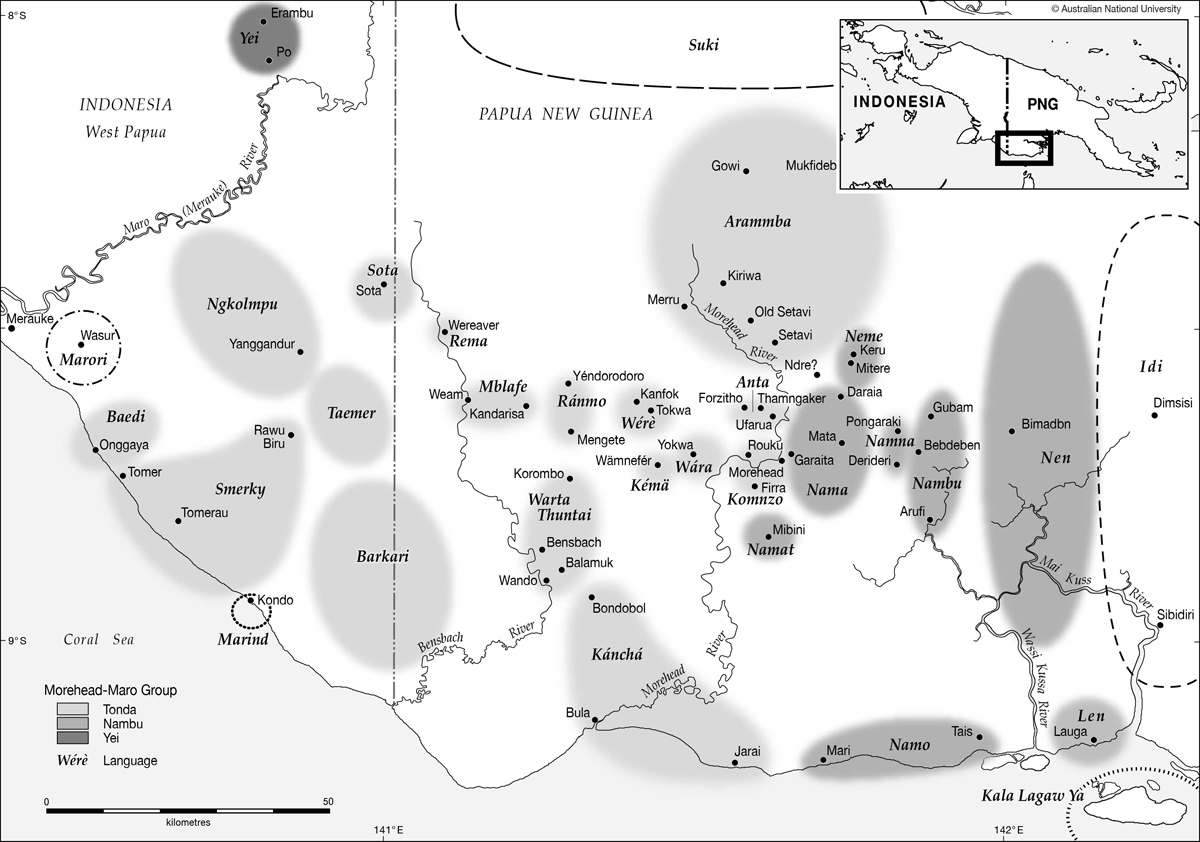
\includegraphics[width=\textwidth]{figures/map1.jpg}
	  \caption[Map of the languages of Southern New Guinea]{Map of the languages of Southern New Guinea}
	  \label{fig-01-SNGmap}
	\end{figure}
\end{landscape}%SNGmap

\section{Typological overview}\label{Typoverview}

\subsection{Introduction}

Komnzo is a Papuan language. The term Papuan is a negative category comprising those languages of the area near New Guinea which are neither Austronesian nor Australian. It was originally introduced by Sidney Ray (\citeyear[24]{Ray:1926papuan}). The number of distinct language families that have been proposed ranges from ten \citep{Wurm:1975etal} to 23 \citep{Ross:2005pronouns} up to 60 \citep[3]{Foley:1986ux}. Although authors acknowledge the incredible diversity within New Guinea, there have been some attempts at defining grammatical properties which are characteristic for Papuan languages (\citealt{Foley:1986ux} and \citealt{Foley:2000uh}). Komnzo, the languages of the Yam family, and possibly the whole Southern New Guinea area deviate from this Papuan type. Other authors have shown that the languages of New Guinea do not share a set of typological features that set them apart from the languages of the world \citep{Comrie:2009vza}.

In the following sections, I will introduce the typologically most striking features of the language. Detailed information on each topic can be found in later chapters.

\subsection{Phonology}

The Komnzo phoneme inventory consists of eight vowels and 18 consonants. The vowels are the five cardinal vowels [i], [e], [a], [ɔ], [u] plus a low front unrounded vowel [æ] and, two front rounded vowels [y] and [œ], which are unusual for Papan languages.\footnote{Outside of the Yam family front rounded vowels are also found in \ili{Awyu-Dumut} languages \citep[60]{vanEnk:1997tl}.} The most frequent vowel is the \isi{epenthetic vowel}, which is \isi{schwa}.

\begin{figure}
	{
		\begin{vowel}[plain]
			\putvowel{i}{0,5\vowelhunit}{0,4\vowelvunit}
			\putvowel{y}{1,0\vowelhunit}{0,4\vowelvunit}
			\putvowel{e}{1,3\vowelhunit}{1,5\vowelvunit}
			\putvowel{œ}{1,8\vowelhunit}{1,5\vowelvunit}
			\putvowel{æ}{2,1\vowelhunit}{2,5\vowelvunit}
			\putvowel{u}{3,7\vowelhunit}{0,4\vowelvunit}
			\putvowel{a}{2,9\vowelhunit}{2,7\vowelvunit}
			\putvowel{(ə)}{2,7\vowelhunit}{1,3\vowelvunit}
			\putvowel{ɔ}{3,7\vowelhunit}{1,5\vowelvunit}
		\end{vowel}
	}%
	\caption{Vowels}
	\label{fig-01-vowels}
\end{figure}%vowels

The consonants follow a set of pairs of voiceless and prenasalised \isi{plosives} at the \isi{alveolar} and \isi{velar} point of articulation: [t], [ⁿd], [k], [{\ᵑ}g]. There are labialised velars: [kʷ], [{\ᵑ}gʷ]. At the bilabial point of articulation there is only a prenasalised plosive [ᵐb], while its oral counterpart [b] only occurs in loanwords. There are three \isi{nasals} [m], [n], [ŋ], one trill/tap [r], two semivowels [j], [w] and, again unusual for Papuan languages, three \isi{fricatives} [ɸ], [ð], [s] and two affricates [ts], [ⁿdz]. It follows that we can identify three main points of articulation: bilabial, \isi{alveolar} and \isi{velar}. Further points of articulation include dental [ð], palato-\isi{alveolar} [ts] and [ⁿdz] as well as palatal [j].

\begin{figure}
	\begin{tabularx}{\textwidth}{XXXXXXX}
		&&t&ts&&k&kʷ\\
		ᵐb&&ⁿd&ⁿdz&&{\ᵑ}g&{\ᵑ}gʷ\\
		m&&n&&&ŋ&\\
		ɸ&ð&s&&&&\\
		&&r&&&&\\
		&&&&j&&w\\
	\end{tabularx}
	\caption{Consonants}
	\label{fig-01-consonants}
\end{figure}%consonants

As in other Papuan languages, for example such as \ili{Kalam} \citep{Blevins:2010ee}, many syllables lack phonemically specified vowels. In this case, an \isi{epenthetic vowel} may be inserted, usually a short central vowel [ə]. Many words lack phonemically specified vowels altogether such as \emph{ymgthkwrmth} [jə̆mə̆{\ᵑ}gə̆θkʷə̆rə̆mə̆θ] `they were feeding him'.

The \isi{syllable} structure allows for complex onsets of the type CRV, as in \emph{gru} `shooting star' or \emph{srak} `boy'. Otherwise onsets are simply CV. Even though vowel-initial words exist, they are always produced with a \isi{glottal stop}, as in \emph{ane} [ʔane] `that' or \emph{ebar} [ʔeᵐbar] `head'. Syllable codas are optional, but they consists of one consonant maximally.

\subsection{Morphology}

Komnzo morphology can be used to easily distinguish \isi{nominal}s from verbs. As in other \ili{Yam languages} such as \ili{Nama} \citep{Siegel:2015bp} and \ili{Nen} \citep{Evans:2015to}, Komnzo \isi{verb} morphology exhibits a high degree of complexity. Verbal morphology is highly synthetic, while \isi{nominal} morphology is almost entirely suffixing.

Komnzo nouns are inflected for \isi{number} if their referent is \isi{animate}. Otherwise \isi{number} marking only takes place in the \isi{verb}. Furthermore, nouns are marked for \isi{case} by enclitics, which attach to the last element of the \isi{noun phrase}. \tabref{tab-01-case} shows the \isi{case} markers for the \isi{inanimate} noun \emph{efoth} `sun, day' and the \isi{animate} noun \emph{kabe} `man, people'.

\begin{table}
\caption{Cases}
\label{tab-01-case}
	\begin{tabularx}{\textwidth}{Xlll}
	\lsptoprule
		&inanimate&animate singular& animate non-singular\\
		\midrule 
		Absolutive&\emph{efoth=\Zero}&\emph{kabe=\Zero}&\emph{kabe=é}\\
		Ergative&\emph{efoth=f}&\emph{kabe=f}&\emph{kabe=é}\\
		Dative&\emph{efoth=n}&\emph{kabe=n}&\emph{kabe=nm}\\
		Possessive&\emph{efoth=ane}&\emph{kabe=ane}&\emph{kabe=aneme}\\
		Locative&\emph{efoth=en}&\emph{kabe=dben}&\emph{kabe=medben}\\
		Allative&\emph{efoth=fo}&\emph{kabe=dbo}&\emph{kabe=medbo}\\
		Ablative&\emph{efoth=fa}&\emph{kabe=dba}&\emph{kabe=medba}\\
		Temporal locative&\emph{efoth=thamen}&n/a&n/a\\
		Temporal purposive&\emph{efoth=thamar}&n/a&n/a\\
		Temporal possessive&\emph{efoth=thamane}&n/a&n/a\\
		Instrumental&\emph{efoth=me}&n/a&n/a\\
		Purposive&\emph{efoth=r}&n/a&n/a\\
		Characteristic&\emph{efoth=ma}&\emph{kabe=anema}&\emph{kabe=anemema}\\
		Proprietive&\emph{efoth=karä}&\emph{kabe=karä}&n/a\\
		Privative&\emph{efoth=mär}&\emph{kabe=mär}&n/a\\
		Associative\super{a}&\emph{efoth=ä}&\emph{kabe=r}&\emph{kabe=ä}\\
		Similative&\emph{efoth=thatha}&\emph{kabe=thatha}&n/a\\
	\lspbottomrule
		\multicolumn{4}{l}{\footnotesize \super{a}The associative forms encode {\Du} versus {\Pl} (\S\ref{inclusorycontruction}).}
	\end{tabularx}
\end{table}%case

Nominal morphology in Komnzo is comparatively simple. Case marking is shown by enclitics that attach to the rightmost element of a noun phrase, which is usually a head noun as in (\ref{exintro2}), but may sometimes be a modifier as in (\ref{exintro3}).

\begin{exe}
	\ex \label{exintro}
	\begin{xlist}
		\ex
		\gll \emph{kafar} \emph{kabe=f=nzo}\\
		big man=\Erg.\Sg=\Only\\
		\trans `only the big man (did sth.)'
		\label{exintro2}
		\ex
		\gll \emph{kabe} \emph{kafar=f=nzo}\\
		man big=\Erg.\Sg=\Only\\
		\trans `only the big man (did sth.)'
		\label{exintro3}
	\end{xlist}
\end{exe}

In contrast to \isi{nominal}s, \isi{verb} morphology is highly synthetic. Verbs may index up to two arguments showing agreement in \isi{person}, \isi{number} and \isi{gender}. Verbs encode 18 TAM categories, \isi{valency}, \isi{directionality} and \isi{deictic} status. Complexity lies not only in the number of categories verbs express, but also in the categories are encoded.

\subsection{Distributed exponence}

Komnzo verbs exhibit what may be called ``\isi{distributed exponence}''. Distributed \isi{exponence} is characterised by the fact that morphemes are underspecified for a particular grammatical category. Therefore, morphological material from different sites has to be taken into account. This phenomenon is different from \isi{multiple exponence} (e.g. circumfixes) in that each morphological site can be manipulated independently. This is shown in \tabref{tab-01-thoraksi} in the expression of a few selected TAM categories for the verb \emph{thoraksi} `arrive, appear' in a third singular masculine frame.

\begin{table}
\caption{Distributed exponence - TAM}
\label{tab-01-thoraksi}
	\begin{tabularx}{.66\textwidth}{Xl}
	\lsptoprule
		non-past imperfective & \emph{y-thorak-wr}\\
		recent-past imperfective & \emph{su-thorak-wr}\\
		recent-past durative & \emph{y-thorak-wr-m}\\
		recent-past perfective & \emph{sa-thor}\\
		past imperfective & \emph{y-thorak-wr-a}\\
		past durative & \emph{su-thorak-wr-m}\\
		past perfective & \emph{sa-thor-a}\\
		iterative & \emph{su-thor}\\
		\lspbottomrule
	\end{tabularx}
\end{table}%thoraksi

Distributed \isi{exponence} means that we cannot \isi{gloss} the prefix \emph{y-} for a \isi{tense} value, because it is used for the inflections of \isi{non-past}, \isi{recent past} and \isi{past}. Furthermore, glossing the suffix \emph{-m} as a \isi{durative} is only half of its function as it backshifts \isi{tense} as well from \isi{non-past} to \isi{recent past} and again from \isi{recent past} to \isi{past} \isi{tense}. In fact, the only morpheme in the example that serves only one function is the \isi{past} suffix \emph{-a}. As we can see in the example, exponents of TAM include the verb stem (\emph{thorak} versus \emph{thor}). Indeed, most Komnzo verbs possess two stems which are sensitive to \isi{aspect}. Again, the stem alone is not sufficient to express the aspectual values (\isi{imperfective}, \isi{perfective}, \isi{iterative}, \isi{durative}), but it is the combination of stem type, prefix and suffix.

Distributed \isi{exponence} is best explained with the way Komnzo marks \isi{number} on verbs. The four possible values are \isi{singular}, \isi{dual}, \isi{plural}, and \isi{large plural}. Note that only a small subset of verbs can form large plurals. The exponents of \isi{number} are distributed over two morphological slots. There is a binary distinction in the prefix (\emph{y-} vs. \emph{e-}) and the suffix (\emph{-thgr} vs. \emph{-thgn}). The four possible combinations of these exponents encode the four \isi{number} values. This is shown with the intransitive verb \emph{migsi} `hang' in a third person frame in \tabref{tab-01-migsi}.

\begin{table}
\caption{Distributed exponence - number}
\label{tab-01-migsi}
	\begin{tabularx}{.5\textwidth}{Xl}
	      \lsptoprule
		\isit{singular} & \emph{y-mi-thgr}\\
		\isit{dual} & \emph{e-mi-thgn}\\
		\isit{plural} & \emph{e-mi-thgr}\\
		\isit{large plural} & \emph{y-mi-thgn}\\
		\lspbottomrule
	\end{tabularx}
\end{table}%migsi

\subsection{Syntax}

Komnzo is a double-marking language. The \isi{case} marking is organised in an \isi{ergative}-\isi{absolutive} system. In addition to three core cases (\isi{absolutive}, \isi{ergative} and \isi{dative}), there are 14 semantic cases. Verbs index up to two arguments. The \isi{undergoer} argument is indexed by a prefix and the actor argument is indexed by a suffix. One-place predicates split along the lines of stative versus dynamic event types. The latter employ the suffix for indexing, while the former make use of the prefix. Valency changing morphology enables the indexing of a \isi{goal}, \isi{beneficiary} or \isi{possessor} in the prefix. This is shown below with the verbs `stand', `return', `see' and `give'. I use the term ``\isi{template}'' to describe the different inflectional patterns in which verb stems are found.

\begin{exe}
\ex
\label{exintro4}
\begin{xlist}
	\ex %\textit{fi ykogr.}\\
	\gll \emph{fi} \emph{y-rugr}.\\
	\Third.{\Abs} \Tsg.\Masc-sleep\\
	\trans `He sleeps.'
	\ex %\textit{fi ŋamränzrth.}\\
	\gll \emph{fi} \emph{ŋabrigwr-th.}\\
	\Third.{\Abs} return-\Tpl\\
	\trans `They return.'
	\ex %\textit{nafa fi yfnzrth.}\\
	\gll \emph{nafa} \emph{fi} \emph{y-mar-th}.\\
	\Tpl{}.{\Erg} \Third.{\Abs} \Tsg.\Masc-see-\Tpl{}\\
	\trans `They see him.'
	\ex
	\gll \emph{nafa} \emph{yare} \emph{kabe=n} \emph{y-a-rithr-th}.\\
	\Tpl{}.{\Erg} bag(\Abs) man={\Dat} \Tsg.\Masc-\Vc-give-\Tpl{}\\
	\trans `They give the man the bag.'
\end{xlist}
\end{exe}

The most frequent word order in Komnzo is \isi{SOV}, more accurately AUV\footnote{AUV: actor undergoer verb.}, since there is only weak evidence for a subject category. At the same time, the flagging of \isi{noun phrase}s with \isi{case} allows for considerable freedom in the word order patterns. Nominal compounds and \isi{noun phrase}s are typically \isi{head}-final, although modifying elements in the \isi{noun phrase}, for example adjectives or quantifiers, may occur after the \isi{head}. Relative clauses follow their \isi{head}.

Subordinate clauses in Komnzo are usually non-finite employing nominalised verbs with appropriate \isi{case} markers. Verb chaining and the distinction between medial and final verb forms, which are typical for Papuan languages, are not found in Komnzo. The examples below show a phasal \isi{complement} (\ref{exintro5}) and a \isi{complement} of desire (\ref{exintro6}).

\begin{exe}
	\ex
	\gll \emph{nafa} \emph{with} \emph{rku-si} \emph{the-thkäfa-th}.\\
	\Tnsg.{\Erg} banana({\Abs}) knock.down-{\Nmlz} \Stpl-start-\Stsg\\
	\trans `They started knocking down the bananas.'
	\label{exintro5}
\end{exe}

\begin{exe}
	\ex
	\gll \emph{fi} \emph{miyo} \emph{yé} \emph{nge} \emph{fatha-si=r}.\\
	\Third.{\Abs} desirous \Tsg.\Masc.be child hold-\Nmlz={\Purp}\\
	\trans `He wants to hold the child.'
	\label{exintro6}
\end{exe}

In addition to nominalised verbs, clauses can be connected with conjunctions (\ref{exintro7}), relative pronouns (\ref{exintro8}) or demonstratives flagged for case (\ref{exintro9}).

\begin{exe}
	\ex
	\gll \emph{fi} \emph{z} \emph{zebnaf}-\Zero{} \emph{o} \emph{komnzo} \emph{y-rugr}?\\
	\Third.{\Abs} {\Iam} wake.up-\Tsg{} or still \Tsg.\Masc-sleep\\
	\trans `Did he wake up already or is he still sleeping?'
	\label{exintro7}
\end{exe}

\begin{exe}
	\ex
	\gll \emph{kabe} \emph{sa-thor} \emph{kayé} \emph{mane} \emph{sf-marwrm-e}.\\
	man(\Abs) \Tsg.\Masc-arrive yesterday which \Tsg.\Masc-see-\Fpl\\
	\trans `The man who we saw yesterday arrived.'
	\label{exintro8}
\end{exe}

\begin{exe}
	\ex
	\gll \emph{ŋare} \emph{z} \emph{ze-far} \emph{bäne=ma} \emph{nafane} \emph{kkauna} \emph{zwa-rithr-th}.\\
	woman(\Abs) {\Iam} \Tsg.\F-set.off \Dem:\Med={\Char} \Tsg.{\Poss} things \Tsg.\F-give-\Tpl\\
	\trans `The woman has left already, because they gave back her belongings to her.'
	\label{exintro9}
\end{exe}

\section{The Farem people and their language}\label{faremlang}

\subsection{Location}\label{location}

The area considered in this study is the southwestern corner of the Western Province of Papua New Guinea. This area used to be called ``Trans-Fly'' in the past, for example in Williams' ethnography of the \ili{Keraki} people entitled ``Papuans of the Trans-Fly'' (\citeyear{Williams:1936transfly}). Mary Ayres rightly criticises this term for its geo-centrism (\citeyear[1]{Ayres:ws}). I use the administrative term ``Morehead district'' which encompasses the area between the Indonesian border to the west, the Fly River to the north, the boundary of the Yam language family in the east (see Figure \ref{fig-01-SNGmap}), and the coastline in the south.\footnote{The Morehead-Rural census division encompasses the same area, but the eastern border is further to the east including some of the \ili{Pahoturi River} languages such as \ili{Idi}.} The area is named after Morehead station, the administrative center, and the Morehead River, which in turn was named after Boyd Dunlop Morehead, the premier of Queensland between 1888 and 1890. I use the term ``Southern New Guinea'' which encompasses a much wider region roughly from the Digul River in the west to the Fly River in the north and east.

Komnzo is spoken in the village of Rouku, which is located about 7km west of Morehead and about a kilometer north of the Morehead River. It is situated on the road that connects Morehead with Weam in the west. Traditional lands expand about 20km east-west and 25km north-south. There are four clans in Rouku village: \emph{Mrzar Mayawa, Banibani Mayawa, Muthrata Sangara, Wazu Sangara}.\footnote{Mary Ayres avoids using the word `clan' (\citeyear[142]{Ayres:ws}), instead she draws a distinction between ``non-local sections'' (\emph{Bagu, Mayawa, Sagara}), which are found throughout the region, and ``local-sections'' (\emph{Nümgar Bagu, Mrzar Mayawa, Muthrata Sangara}), which are found in one group only, for example the Farem. I will use `clan' for the latter and `section' for the former. This is discussed in \S\ref{exogamy}.} Further settlements include Morehead, Gunana, Firra, Kanathr, Ŋazäthe and Masu. Only Morehead and Gunana are settled permanently, while the others are garden places in some years. The map in Figure \ref{fig-01-ROUKUmap} shows Rouku and the surrounding places.

\begin{figure}
    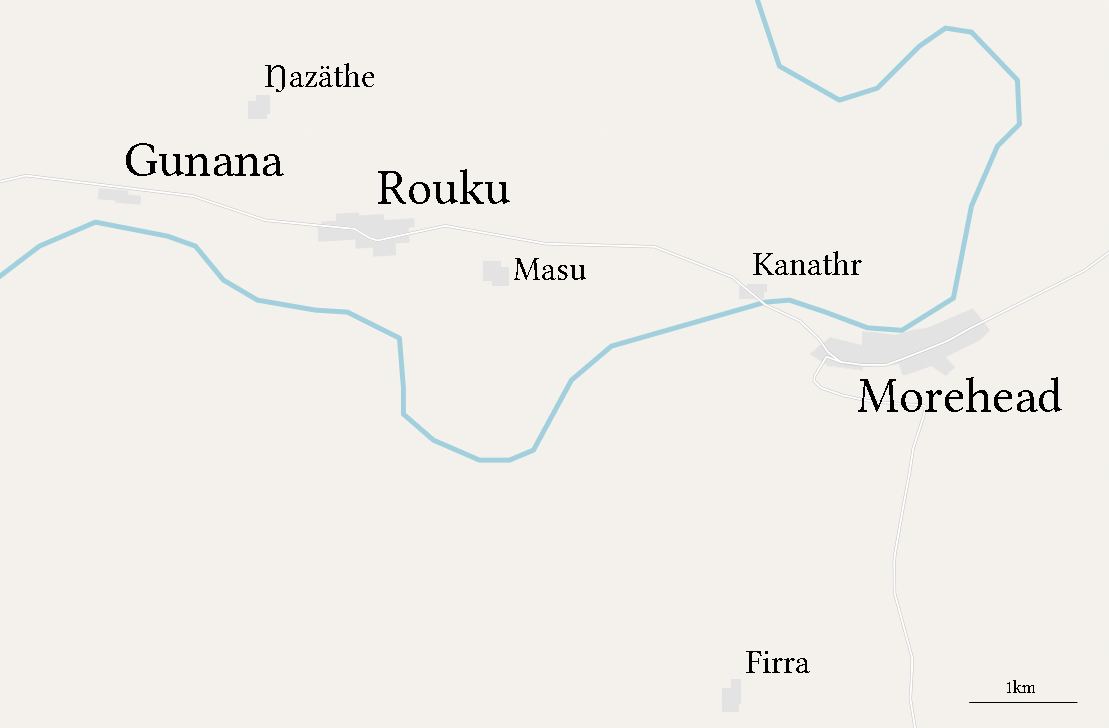
\includegraphics[width=.9\textwidth]{figures/map2.png}
  \caption[Rouku]{Rouku and surrounds}
  \label{fig-01-ROUKUmap}
\end{figure}%rouku

Gunana, the second largest settlement, is situated about 2km west of Rouku along the road. The present-day village was established around 10 years ago. Gunana is situated closer to the Morehead River. The name Rouku, from the Komnzo word \emph{rokuroku} `riverbank', was given to this place when the first missionaries arrived in the 1950s. Thus, Gunana is the original Rouku, and it is often referred to as Rouku-Gunana. The word \emph{gunana} is a \isi{loanword} from Motu which means `old'. Two clans live in Gunana today: \emph{Farem Sangara} and \emph{Nümgar Bagu}. They speak mostly \ili{Wára} and \ili{Anta} for reasons which I address in {\S}\ref{ideomulti}. Morehead station includes the government administration, the aidpost, the primary school and the airstrip. A number of small settlements are built around Morehead station, and these virtually merge into one another. The largest of these is Garaita, a \ili{Nama}-speaking village. Since Morehead station was built on land belonging to the Mayawa section from Rouku, some families from Rouku have settled in Morehead permanently. One small hamlet of this kind is Fsan. Moreover, some families from Rouku live in Morehead because they are employed in the local administration as teachers or public servants. With respect to clans, this population is mixed. The hamlet Firra is situated about 7km south of Morehead. Only a few families of the \emph{Banibani Mayawa} clan live there. Most of the people have shifted their residence to Morehead, but keep garden places at Firra. Kanathr is a small hamlet located 2km west of Morehead on the northern side of the river. Kanathr marks the point where the road crosses the river. As there is no bridge, people cross the river by canoe, and cars or motorcycles use a rusty old pontoon. Kanathr serves as a place where children from Rouku and Yokwa, the next village along the road to the west, stay overnight while they attend Morehead primary school. Kanathr was settled in the 1980s, and deserted in the 1990s, and has only been re-established over the last three years. Its population is mixed with respect to clans, but since the land belongs to the two Mayawa sections, they make up the majority.

There are many places around Rouku that used to be settled, but have now been abandoned or are used only as garden places. These include Ytkum, Dmädr, Faremkar, Ŋazäthe, Masu and Akrimogo. Two examples are Ŋazäthe and Masu. The map in Figure \ref{fig-01-ROUKUmap} shows Ŋazäthe, Rouku and Masu. Both used to be settled until about 10 years ago by clans of the \emph{Sagara} and \emph{Mayawa} section respectively. Today both are used as garden places, but they still play an important role as places of origin. Both places are very close to Rouku, about a 15-minute walk. Note that named places are densely clustered in the Morehead district, especially in the vicinity of settlements. More importantly, these places are perceived as being different despite their geographic proximity. This topic is discussed in \S\ref{placenames}.

\subsection{Geography and environment}\label{geographyenviro}

In its biota, the Morehead district is more similar to northern Australia than to the rest of New Guinea. We find eucalypts, melaleuca, acacias and banksias combined with wallabies, bandicoots, goannas, taipans and termite mounds. The area consists of lowland which a Papuan highlander or a European would describe as almost featureless. An early visitor, Wilfred Norman Beaver, concluded that ``there is nothing to induce settlement, nor would I ever advice anyone to go there.'' \citep[64]{Murray1912pap}. Francis Edgar Williams described the landscape as having a ``mild, almost dainty, attractiveness in detail, but [...] on the whole the extreme of monotony'' (\citeyear[1]{Williams:1936transfly}).

\begin{figure}
    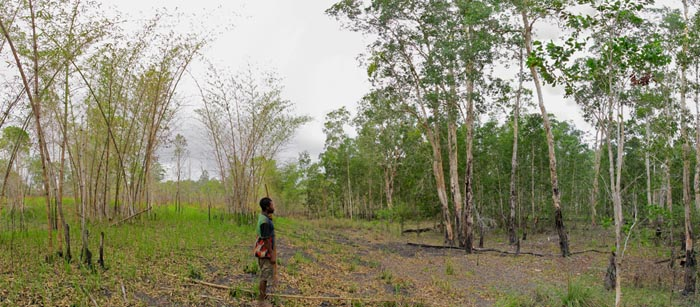
\includegraphics[width=.9\textwidth]{figures/landscape1.jpg}
  \caption[The highest water level during wet season]{Rouku: the area to the right is inundated during wet season}
  \label{fig:landscape1}
\end{figure}%water level

I have measured differences in elevation between 12m and 41m above sea level.\footnote{This was done with a GPS device: the 12m point was the water-level of the Morehead River close to Rouku; the 41m point was measured in Rouku village.} However small these differences in elevation, they are significant over the monsoon cycle with a long dry season (June - November) and an intense wet season (January - May). Areas very close to settlements or gardens are inundated during the wet season, while the larger villages are situated on higher ground. In fact, all villages along the road are built on what is called the ``Morehead ridge'' (\citealt[15]{Paijmans:1971morehead}), thus keeping houses and gardens safe from the annual flooding. The photo in Figure \ref{fig:landscape1} was taken in Rouku. During the previous wet season, the paperbark trees to the right were inundated to about 1m, while the bamboo groves on the left stayed dry.

The Morehead ridge is intersected by many small creeks, which carry little or no water during the dry season. The Morehead River always carries water as it slowly meanders towards the coast. The Morehead forms a narrow, deep channel whose riverbanks drop off sharply 2-3m down to the water level. Close to Rouku village, I have measured 40m width and 15-20m depth during the dry season. The Morehead is a tidal river, which means that during the dry season, when it has virtually no flow, salt water pushes back many kilometers upriver. During the wet season, the river overflows and turns the surrounding land into a wide swamp with many inlets and lagoons. See also Hitchcock (\citeyear[100]{Hitchcock:2004vk}) for a description of the ecology of the region. \figref{fig:landscape2} shows the Morehead River during the dry season.

\begin{figure}
    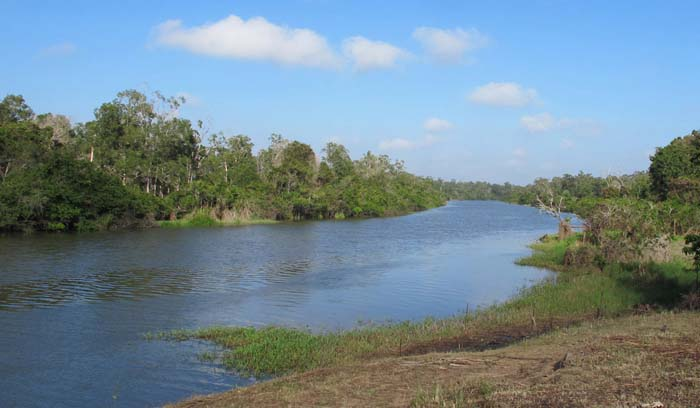
\includegraphics[width=.9\textwidth]{figures/landscape2.jpg}
  \caption[Morehead River]{The Morehead River near Rouku during dry season}
  \label{fig:landscape2}
\end{figure}%morehead river

There is a remarkable diversity of ecological zones (\citealt{Paijmans:1970bl} and \citealt{Paijmans:1971morehead}). For the description of native land use, Ayres distinguishes four \isi{landscape} types: ``big bush'', ``open bush country'', ``clear places'', and ``seasonal swamps'' (\citeyear[5]{Ayres:ws}). In what follows, I employ the respective Komnzo terms: (i) \emph{kafar fz} `big forest', which is a type of monsoon rainforest, (ii) \emph{fz} `forest', which is a much thinner forest type covered by a grass floor and dotted with red anthills, (iii) \emph{ksi kar} `bushy place', which is a type of savannah that lacks trees, but is covered with high grass, and (iv) \emph{zra} `swamp', which is a place entirely inundated during the wet season timbered by paperbark trees and a ground cover of dead leaves. Figures \ref{fig:landscape3}-\ref{fig:landscape6} show images of these types in the vicinity of Rouku village. As one would expect, these \isi{landscape} types differ strongly in the kinds of plants that grow there. The collection of specimens and their identification was greatly facilitated by Kipiro Damas, who visited Rouku in 2011 and 2015.

The Morehead district is rich in wildlife. The main game species are pigs, cassowaries and wallabies. There are many other marsupial species including bandicoots, phalangers (cuscus) and gliders. The Morehead district is also abundant in birdlife. Attested species include birds of paradise, parrots, lorekeets, pidgeons, eagles, hawks, bush fowls, jaberoos, storks and brolgas. Thanks to the help of Chris Healey, who visited Rouku in 2012 and 2013, we were able to match around 100 Komnzo bird names to the corresponding scientific names of these species. The rivers and swamps are rich in fish and amphibious species, for example barramundis, mullets, catfish, eelfish, rainbowfishes, glassfishes, stingrays, river crayfish, prawns, crocodiles, water snakes and turtles. Other reptiles include various goanna species, frogs and snakes. Examples for the latter are the Papuan taipan, the New Guinea death adder, the New Guinea brown snake, the Papuan blacksnake as well as various python types.

\begin{figure}
    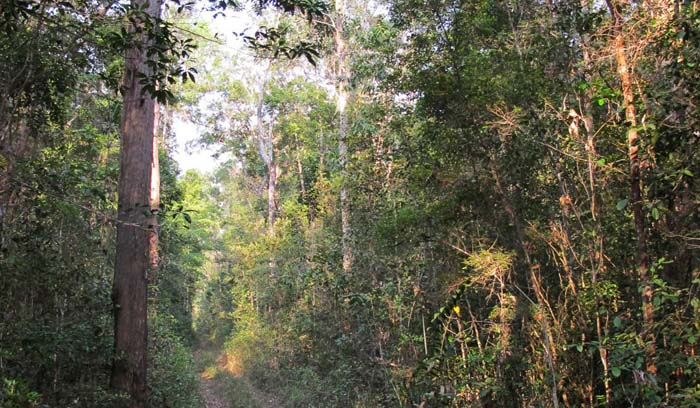
\includegraphics[width=.9\textwidth]{figures/landscape3.jpg}
  \caption[\emph{Kafar fz}: monsoon rainforest (with a road)]{\emph{Kafar fz}: road cut through the monsoon rainforest}
  \label{fig:landscape3}
\end{figure}%kafar fz

\begin{figure}
    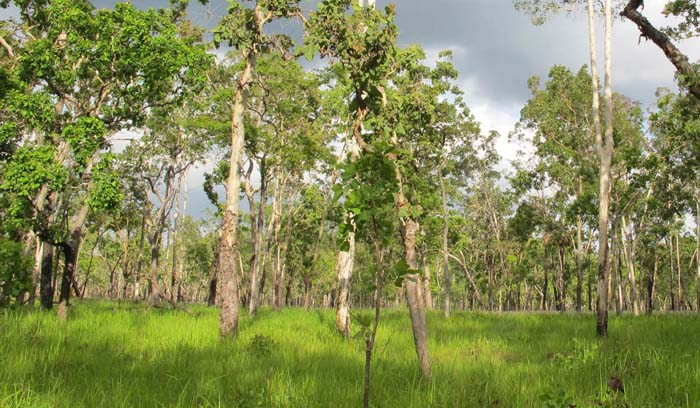
\includegraphics[width=.9\textwidth]{figures/landscape4.jpg}
  \caption[\emph{Fz}: thin forest]{\emph{Fz}: thin forest}
  \label{fig:landscape4}
\end{figure}%fz

\begin{figure}
    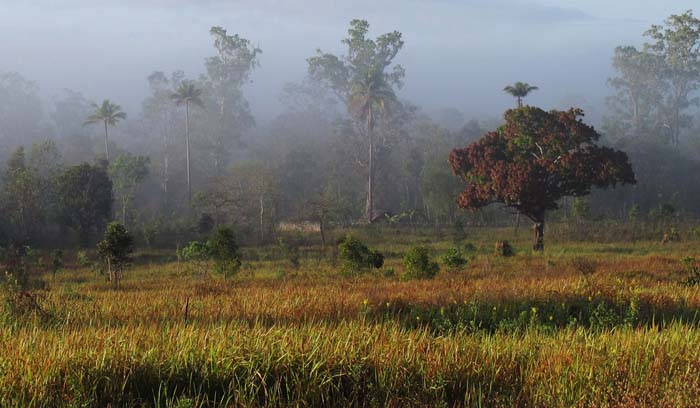
\includegraphics[width=.9\textwidth]{figures/landscape5.jpg}
  \caption[\emph{Ksi kar}: small patch of savannah]{\emph{Ksi kar}: small patch of savannah}
  \label{fig:landscape5}
\end{figure}%ksi kar

\begin{figure}
    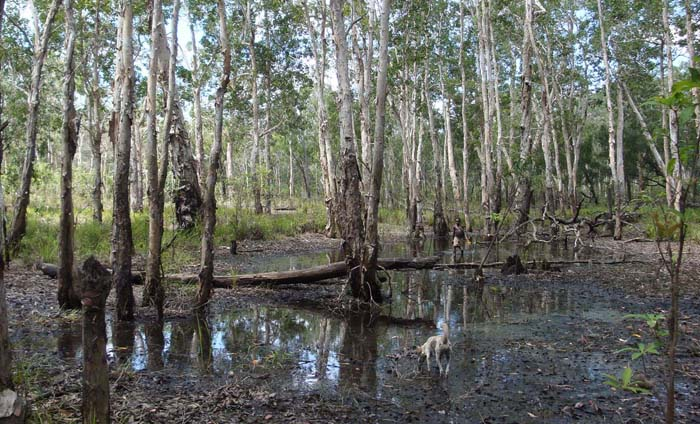
\includegraphics[width=.9\textwidth]{figures/landscape6.jpg}
  \caption[\emph{Zra}: seasonal swamp during dry season]{\emph{Zra}: seasonal swamp during dry season}
  \label{fig:landscape6}
\end{figure}%zra

\subsection{Agriculture and subsistence}\label{agriculture}

The Farem people are agriculturalists. Their main crops are round and long yams, bananas, sweet potatoes, cassava, taro, coconut, sago, breadfruit and sugar cane. Additionally, there are many fruits and nuts available during the dry season. Although the Farem are skilled in hunting, trapping and fishing, they rely on their garden products. In this section, I will focus on their staple food: yam.

\begin{figure}
    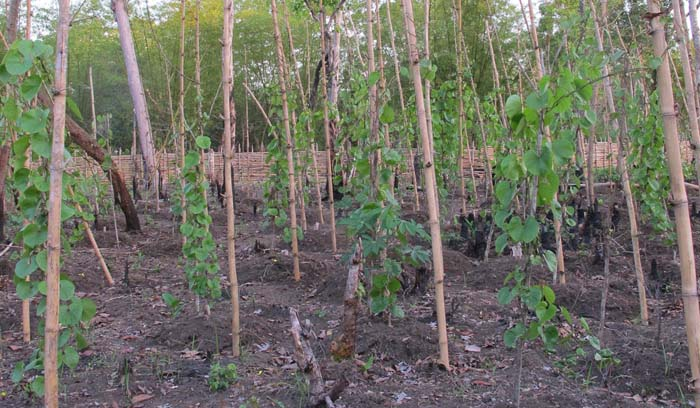
\includegraphics[width=.9\textwidth]{figures/yam1.jpg}
  \caption[Yam garden two months after planting]{Yam garden two months after planting}
  \label{fig:yam1}
\end{figure}%yam garden

Without a doubt yams are the most important crop for the Farem, and the role of this bland tasting tuber can hardly be overstated. Williams concludes his chapter on food production by stating that ``the social significance of food among these people derives largely from the pride which individuals and groups feel in having plenty of it.'' (\citeyear[235]{Williams:1936transfly}). Large quantities of yams are exchanged at feasts, and sizeable tubers are often given as personal gifts. During the celebration of Independence Day in Morehead, there is a competition where individuals measure and weigh their biggest yams. On many occasions, people have shown off the content of their yam houses to me, and during harvest time some of my friends have peeked through the wall of other's yam house to examine the yield and compare it to their own, which would often become the talk of the day. In short, yams indicate a person's wealth and social status.

Yam cultivation involves hard labour. The cultivation cycle can be divided into three phases: (i) preparing and planting, (ii) tending, and (iii) harvesting. The preparations begin by clearing the land (between August and October). Good, well-drained soil is found on the high ground; either virgin forest or a piece of land that has lain fallow for some years. The gardener has to cut the overgrowth and clear the grass. Large trees are usually only ring-barked and one would wait for the tree to die and eventually to fall. The cleared area has to be burned. Depending on the quality of the soil, one may bring grass from elsewhere and burn it as fertiliser. The ground has to be ploughed thoroughly, and small roots and weeds are pulled out. Next, the garden plot has to be enclosed by a fence to keep out wallabies, deer and wild pigs. The most important material for fences is bamboo which is grown in small bamboo groves. During preparation, people are busy in their gardens every day. Planting may start as early as October, but it can last until January. Yams for planting are selected carefully, but the tiny yam suckers are usually planted in heaps in an old garden plot. Figure \ref{fig:yam1} shows a yam garden about two months after planting. Between January and June, there are many small jobs to be done. These include weeding or erecting and replacing yamsticks on which the vines climb up. The change of the season in June is also signalled by the changing colour of the yam leaves. Around this time, the harvest season begins, and it may stretch until August, when the cycle begins again. Harvested yams are counted, sorted and stored in yam houses. This involves shaving the shoots off each tuber; a time-consuming task that is usually done in the afternoon hours while sitting in conversation in front of the yam house. Because garden plots are subdivided into rows, one for each member of the family, the yams are sorted accordingly in the yam house. Figure \ref{fig:yam2} shows the inside of a yam house after the harvest.

\begin{figure}
    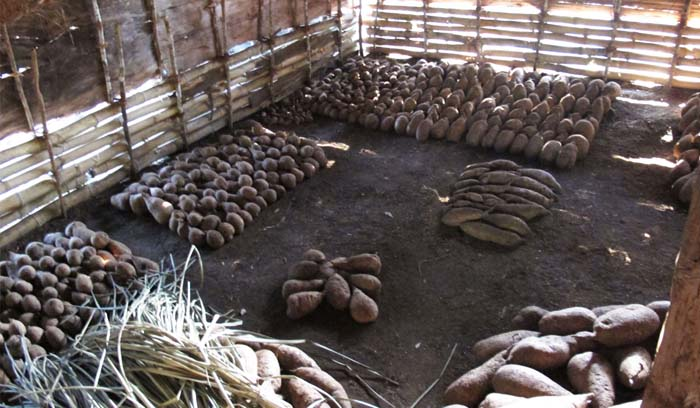
\includegraphics[width=.9\textwidth]{figures/yam2.jpg}
  \caption[Inside a yamhouse]{Inside a yamhouse}
  \label{fig:yam2}
\end{figure}%yam house

There are many special customs around yam cultivation. Some men possess yam planting magic which helps them to compete with others. This usually involves particular spells and magic stones passed down from the father's generation. Others ``steal the soil'' from their competitors. Knowledge of this kind is usually kept secret and never admitted in public. Furthermore, there are a number of rules about handling yams, which everyone follows. One example is the belief in ``female pollution'', which is widespread in Southern New Guinea (\citealt[104]{Knauft:1993south}). During a woman's monthly period, but also after having sexual intercourse, it is strictly forbidden to go to the garden plot for it will ``spoil'' the yams. This rule applies not only to the woman, but to anyone who sleeps in the same house, sometimes even the neighbouring house.

Yams play the most important role in exchange feasts. For example, an exchange marriage is consummated through a feast, sometimes called ``pig dance''. The two men who have exchanged sisters henceforth \emph{fäms} `exchange fellow', will raise a pig and invite their respective \emph{fäms} and his associates for a dance. The host side will feed the guests, and in return the guests will entertain the hosts by singing and dancing through the night. The next day, the hosts will give the guests large quantities of yam tubers to take back to their village. The amount has to be recorded with great detail, because after a year has passed, the roles will be reversed. Nothing would be more embarrassing than falling short in the repayment. Often two villages have particularly strong marriage links. In the past this has led to competitive yam cultivation between the two groups.

Yams also play a role in the regulation of conduct. I have been told about a ritual called \emph{mefa}. The culprit, usually someone who has treated his wife badly, is confronted by his \emph{fäms} and other brothers of his wife (\emph{ngom}). They will then put lime on the culprit's forehead and then strike him over the head with a small yam tuber. This is, however painful, only an immediate punishment. The bigger punishment comes in the form of a gift. The culprit is given a large quantity of yams, and it is expected that he repays the same amount and quality the next year. An individual can never achieve this, and thus the culprit is forced to ask people in and maybe even beyond his clan for help. If he fails to repay the expected amount, he will lose all respect and social status. Disputes about an individual's gardening abilities may become violent. The only time I had to witness a violent outbreak by one of my brothers, who is a calm and peaceful person, was when his aunt insulted him by accusing him of ``being lazy'' and a ``bad gardener''. After a tirade of insults, this was the last straw. In conclusion, it is difficult to find any aspect of life in which yam cultivation does not play some role.

\subsubsection{Yam counting}\label{yamcounting}

For many of the customs described above, it is important to record the exact quantity of tubers. For the counting ritual a special base-six \isi{numeral system} is used, which is unique to the \ili{Yam languages}. This \isi{senary} system has received some attention in the literature (\citealt{Donohue:2008bn}, \citealt{Hammarstrom:2009bp} and \citealt{Evans:2009wg}). Williams was the first to describe the counting procedure, but he points out that it ``is apparently a more or less recent fashion among the \ili{Keraki}, having been imported from beyond the Morehead'' (\citeyear[225]{Williams:1936transfly}). This area includes the Farem territory. In the following section, I describe the procedure as I have witnessed it many times in Rouku and surrounds.\footnote{I have published two videos of the counting procedure. The interested reader can view them at the following URLs:  {\url{https://zenodo.org/record/1404789}} and {\url{https://zenodo.org/record/1208073}}}

\begin{figure}
    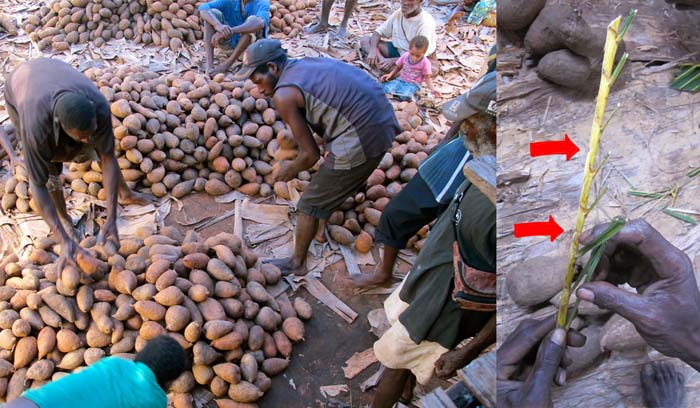
\includegraphics[width=.9\textwidth]{figures/yam3.jpg}
  \caption[Ritual yam counting]{Ritual yam counting (left); counting tally \emph{tiftif} (right)}
  \label{fig:yam3.jpg}
\end{figure}%yam counting

The counting procedure involves two men who move the yam tubers from a prepared pile. They take up three yams each, move a few meters and deposit them together in a new pile. One of the two is the designated counter and he shouts out \emph{näbi näbi näbi} `one one one'. This means that they have moved the first unit of six. Without pause they take up again three yams each and move them over, while the counter shouts out \emph{yda yda yda} `two two two'. Now two lots of six or 12 tubers have been counted. Again they pick up three yams each shouting \emph{ytho ytho ytho} `three three three'. The two men continue with this process until they reach \emph{nibo} `six'. Now 36 yams have been counted and the bystanders and observers cheer in agreement. This amount corresponds to one \emph{fta} or 6\textsuperscript{2}. Each \emph{fta} is marked by putting a single yam on the side of the new pile. The two men continue until all yams have been counted, and the little pile on the side which indicates the amount of \emph{fta} slowly grows. Next, this pile is counted in the same fashion, only that each counting yam, that is put to the side, now markes one \emph{taruba}, which corresponds to 216 or 6\textsuperscript{3}. One may continue in the same fashion. Six \emph{taruba} make up one \emph{damno} corresponds to the amount 1,296 or 6\textsuperscript{4}. For example, one \emph{damno} is amount of yams that a man should store in order to bring his family through the year. Six \emph{damno} make up one \emph{wärämäkä} corresponding to 7,776 or 6\textsuperscript{5}. Finally, six \emph{wärämäkä} make up one \emph{wi} corresponding to 44,656 or 6\textsuperscript{6}. I should add that nobody in Rouku remembered the last time this number was actually reached. The recursive counting procedure gives rise to the \isi{senary} system. I describe the \isi{numeral system} in \S\ref{numerals-subsec}.

Figure \ref{fig:yam3.jpg} shows two men during the counting the procedure. The counting is always a public event accompanied by the loud, monotonous beat of a drum. I was told that neighbouring villages or travellers should be made aware of the ongoing counting procedure. In order to record and keep the amount for later proof, the Farem produce a counting tally made from a coconut frond. This is shown on the right side of Figure \ref{fig:yam3.jpg}. The stalks indicate the number of different \isi{senary} values, which are separated by small notches. The red arrows in the image point to the two notches. Figure  \ref{fig:yam3.jpg} was taken during a yam counting ritual in Morehead in September 2010. The amount counted was 3 \emph{damno}, 2 \emph{taruba}, 3 \emph{fta} or 4,428 tubers in total. This was the contribution of several clans to a pig dance that took place two weeks afterwards in Garaita. The counting had to be repeated two times because older men who observed the procedure closely said that mistakes had been made.

The largest amount of yams that I have seen was in the village of Yokwa in September 2013. Following the death of an older man, his relatives decided to built a \emph{sirä mnz}, a communal yamhouse.\footnote{Mary Ayres uses the word \emph{kwitenz} for this, but my informants from Rouku and Yokwa did not know the word. They suggested \emph{sirä mnz} `\emph{sirä} house'. The word \emph{sirä} refers to the shelves that are found in these yam houses to hold especially large tubers.} All the relatives of the deceased man, including my brother from Rouku, stored several \emph{fta} up to one \emph{taruba} of yams inside this house. The content was to be shared and exchanged during a feast in honour of the deceased at the height of the rainy season. Mary Ayres describes this practice in her chapter on mourning customs (\citeyear[289]{Ayres:ws}). The yamhouse in Yokwa can be seen in \figref{fig:yam4}. It measured 2,50m wide, 1,60m high and an astonishing 60m long. The floor was separated into compartments of equal size where each contributor stored his share. For some of the contributors there was a display shelf (\emph{sirä}) for very large yams. I did not witness the whole counting procedure as it took more than a day, but I estimate that the \emph{sirä mnz} held more than 10,000 yams.

\begin{figure}
    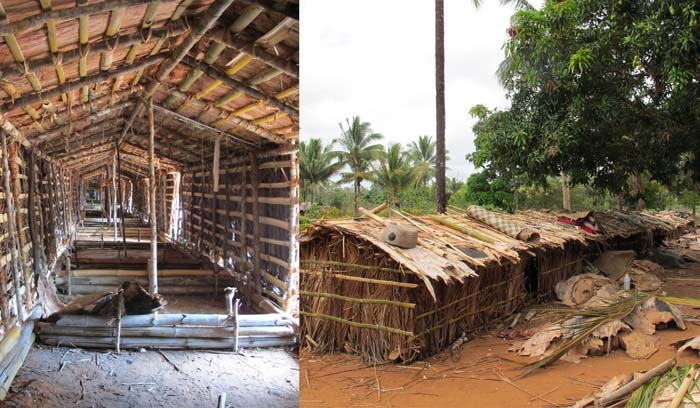
\includegraphics[width=.9\textwidth]{figures/yam4.jpg}
  \caption[Communal yamhouse in Yokwa]{Communal yamhouse in Yokwa: inside (left) / outside (right)}
  \label{fig:yam4}
\end{figure}%sirä mnz

\subsection{Demography and vitality}

It proves difficult to determine the exact number of Komnzo speakers. I give a rough estimate here of about 150 to 250. For the most part, this inexactness is caused by particular social factors. For example, the system of exchange marriage fosters a high degree of \isi{multilingualism}. A Farem child typically grows up speaking at least the varieties of her father and mother. Since the system of residence is virilocal only the father's language is Komnzo. Of course there are two sides to this, and there are many speakers of Komnzo in other villages, namely women who have married out and their children. What complicates matters further in the case of Rouku is that not all Farem men speak Komnzo as their daily language, and not all families have a Komnzo-speaking parent. I provide an explanation for this in {\S}\ref{modernhistory}. Furthermore, there is a small group of speakers who have moved further away to Daru, Kiunga, Port Moresby or other parts of Papua New Guinea.

Komnzo is vital in the sense that the language is being transmitted to children. At the same time, Komnzo is an endangered language because of its small number of speakers and its relatively low prestige compared to the lingua franca, which is \ili{English}. Komnzo is not taught in the school system; there is no writing tradition, and it is not used in administration. For these reasons, it should be regarded as an endangered language from an academic point of view.

Komnzo speakers perceive their language to be under threat from what they call ``mother's language''. Mary Ayres notes that there are strong marriage links between particular villages because it is desirable for a daughter to marry back to her mother's village (\citeyear[226]{Ayres:ws}). In the case of Rouku, there are strong links to Yokwa, and what is meant by ``mother's language'' is almost always \ili{Wára}. One line of reasoning about the perceived threat is that women from Yokwa fail to pass Komnzo on to their children. It should be noted that women are expected to switch their speech variety when they move to their husband's village. In reality this hardly ever occurs, because there are enough women from Yokwa to form small exclaves of \ili{Wára} speakers. Moreover, all Komnzo speakers are fluent in \ili{Wára}. Hence, there is little pressure on a woman to actually change her speech variety. This is different with women who come from more distant places. I discuss the topic of \isi{multilingualism} and \isi{language ideology} in {\S}\ref{ideomulti}.

\subsection{History}\label{history}

\subsubsection{Pre-contact history}\label{prehistory}

Until the rise of the sea level during the Late Pleistocene, the island of New Guinea and the Australian continent were joined in a single landmass called Sahul (\citealt{White:1982prehist}). Recent studies have highlighted that there is still a lack of research from the Southern New Guinea region (\citealt{Pawley:2005ue}, \citealt{Ballard:2010cd}, and \citealt{Evans:2012wp}). The geomorphological past of this lowland region has been turbulent over the last 20,000 years. A chronology of the changing coastlines is given by Chappell (\citeyear{Chappell:2005coastal}).\footnote{His methodology is as follows: ``the procedure for reconstructing the coastlines at a given epoch is to compute the relative sea level field for a given region [...] by combining the ice-equivalent sea level with the regional departures that arise from the isostatic and gravitational factors. The results are then superimposed on the present topography in detail...'' (\citeyear[529]{Chappell:2005coastal}).} Figure \ref{fig:figures_chappell21k} shows the northern coastline of Sahul at the Last Glacial Maximum at 21,000 BP. Figure \ref{fig:figures_chappell8k} shows the coastline at 8,000 BP shortly after the sea breached the Torres Strait, thus disconnecting New Guinea and Australia. The thin black line shows the present coastline.

\begin{figure}
    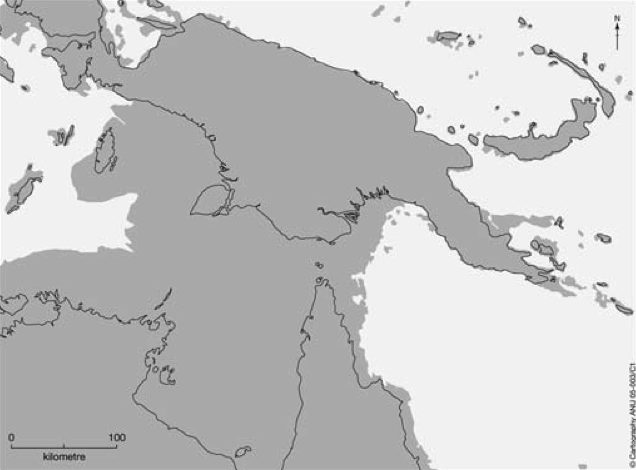
\includegraphics[width=.6\textwidth]{figures/chappell21k.png}
  \caption[Coastline at 21,000 BP]{Coastline at 21,000 BP; adopted from (\citealt[527]{Chappell:2005coastal})}
  \label{fig:figures_chappell21k}
\end{figure}%chappell21

\begin{figure}
    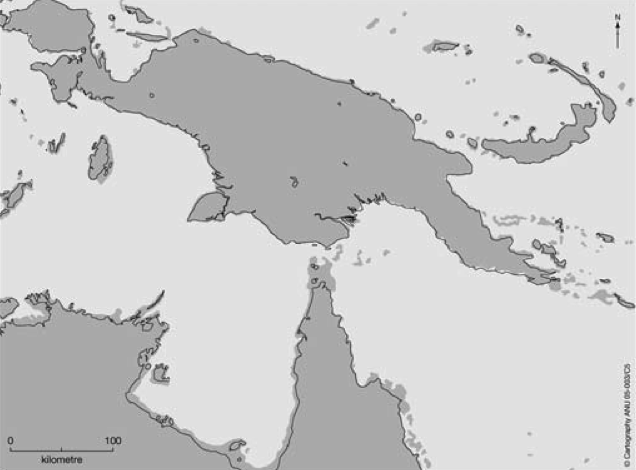
\includegraphics[width=.6\textwidth]{figures/chappell8k.png}
  \caption[Coastline at 8,000 BP]{Coastline at 8,000 BP; adopted from (\citealt[528]{Chappell:2005coastal})}
  \label{fig:figures_chappell8k}
\end{figure}%chappell8

We can see from the figures that the separation of Sahul occurred only shortly before 8,000 BP. Keeping in mind that human presence on the Sahul continent goes back to at least 40,000 BP (\citealt{Golson:2005intro}), we can safely assume that what was later to become the Southern New Guinea region was already settled well before the separation. Chappell shows that large parts of the Fly-Digul platform, to which the Morehead ridge belongs, was submerged at the maximum height of the sea level at 6,000 BP. Figure \ref{fig:figures_chappell6k} shows that this has affected the western part of the Southern New Guinea region.\footnote{With regard to Figure \ref{fig:figures_chappell6k}, which is the result of a computer model, Chappell argues for a more conservative estimate, in which the coastline at 6,000 BP does not extend all the way up to the Fly River (\citeyear[531]{Chappell:2005coastal}).} This part of the region was slowly rebuilt by the sediments carried by the Fly River and Digul River. Note that the Morehead ridge as one of the highest points of elevation on the Fly-Digul platform was not submerged during this period.

\begin{figure}
    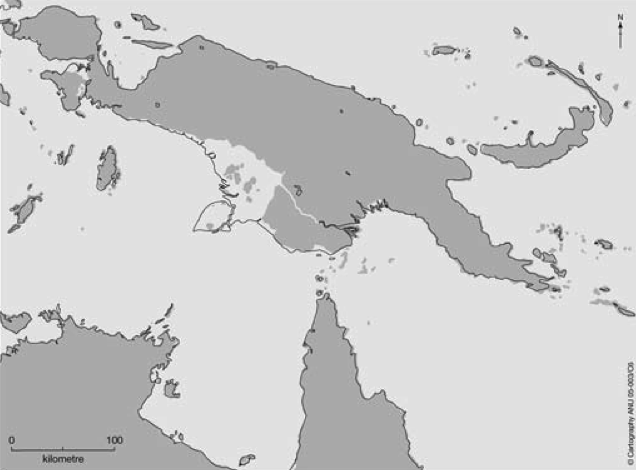
\includegraphics[width=.6\textwidth]{figures/chappell6k.png}
  \caption[Coastline at 6,000 BP]{Coastline at 6,000 BP; adopted from (\citealt[528]{Chappell:2005coastal})}
  \label{fig:figures_chappell6k}
\end{figure}%chappell6

The geological scenario outlined by Chappell is reflected to some extent in the linguistic landscape of the region. For example, concerning the Trans-New-Guinea languages spoken in the west of the Fly-Digul platform, Pawley points out that the ``homogeneity of the Asmat-Kamoro group is clear evidence that their expansion was comparatively recent'' (\citeyear[10]{Pawley:2005intro}). Usher and Suter (\citeyear{Usher:2015kr}) have recently shown evidence for the existence of the Anim language family which stretches from Ipiko in the east to \ili{Marind} and Yaqayic in the west, thus encircling the area under investigation in this study. Evans argues that it is ``unlikely that all language differences currently found in Southern New Guinea developed in situ. What seems more likely is that they represent the interaction of a number of unrelated groups entering the region from different regions'' (\citeyear[111]{Evans:2012wp}). While this is evident for some of the linguistic units, for example the Trans-New-Guinea languages, we do not know how other linguistic units, for example the \ili{Yam languages} or the \ili{Pahoturi River} languages, fit into the chronology of events. I suggest that we should accept the possibility that the \ili{Yam languages} represent a much older population, and {\textendash} as Evans rightly point outs {\textendash} we can only speculate from where this population entered the region.

Some suggestions come from recorded mythology, namely the myth of two brothers and the origin of people at a place called \emph{Kwafar}. This myth was recorded by Williams (\citeyear[306]{Williams:1936transfly}) as well as Ayres (\citeyear[50]{Ayres:ws}). I have recorded a version of this myth told in Komnzo, which is given in the Appendix \ref{kwafar}. What is noteworthy about the story is that the place \emph{Kwafar} is located off the coast in an area that was last exposed well before 8,000 BP. According to this story, there was a flood, and one of the brothers escaped northward. Eventually, he picked up the branches of \emph{dödö} `Melaleuca sp', beat the water with it, and the flood came to a halt. The myth suggests that the people retreated northwards from the rising sea level, i.e. the myth ``reports'' events which date back at least 8,000 years. Although I am not claiming linguistic continuity from the time of the sea level rise to present-day Komnzo {\textendash} after all we know that populations may change languages {\textendash} one cannot deny the fact that this myth is found in the area where the \ili{Yam languages} are spoken, more precisely the languages of the \ili{Tonda} subgroup.\footnote{Both Williams and Ayres recorded these myths with speakers of Tonda languages. Among the origin myths of the Morehead district, this particular myth is only found in Tonda-speaking territory.}

\subsubsection{Modern history}\label{modernhistory}

The Southern New Guinea region was contacted relatively late, which led Knauft to claim that it has ``remained effectively outside the purview of state political economies for longer than any other major non-arctic coastal population'' (\citeyear[26]{Knauft:1993south}). In 1890, Sir William MacGregor, the Administrator of Papua, discovered the Morehead River on an expedition. It took another six years for a second visit by MacGregor during which he collected a vocabulary list, which can be found in the Annual Reports (\citealt[106]{MacGregor:1896rep}).\footnote{Based on the verb forms in the list, I identify the variety as either \ili{Kánchá} or \ili{Kémä}. Nominalised verbs in these two varieties end in a bilabial fricative, and many verbs in the list have a final grapheme <p>. In Komnzo, \ili{Wára}, \ili{Anta} and \ili{Wèré} nominalised verbs end in a vowel: [i] or [e].} Both expeditions travelled by ship. The first known white man to walk through the region was William Dammköhler in 1898 on an adventurous escape from \ili{Marind} headhunters (\citealt{Hitchcock:2009gg}). Until 1921, sporadic patrols were conducted by A. P. Lyons, Resident Magistrate of the Western Division. Lyons recorded native customs, but his journals held at the National Cultural Council at Port Moresby were inaccessible to me. In 1926, F. E. Williams started to pay regular visits to the Morehead district in his role as ``official government anthropologist''. Until 1932, he visited the area almost every year, and his fieldwork culminated in the book Papuans of the Trans-Fly (\citealt{Williams:1936transfly}), which is still the most comprehensive ethnographic description of a group in the Morehead district.

At the time of contact, Southern New Guinea was home to groups of very different sizes and political organisation. On the one end of the spectrum, there were small groups like the Farem, probably with no more than 100 people at that time. On the other end, we find large groups like the \ili{Kiwai} (9,700), \ili{Marind} (7,000) and \ili{Suki} (3,500). Note that these three groups surround the area concerned with in this study. Although headhunting was practised by all groups, it was only those larger groups which could muster war parties and attack places far away from their home territory. This was especially true of the \ili{Marind} (also known as Tugeri or Tugere). In his introduction to Williams' book, AC Haddon, who had led the British expedition in the Torres Strait in 1888, writes that he had ``heard lurid stories about these head-hunting, cannibal marauders'' (\citeyear[xxiiv]{Williams:1936transfly}). The \ili{Marind} were militaristic expansionists, who went on headhunting expeditions raiding villages along the south coast as far as Boigu Island. Since the \ili{Marind}'s home territory was in Dutch New Guinea, the British colonial administration was unable to act against them. The \ili{Marind}'s activity led to a joint Dutch-British expedition, which established the border at the mouth of the Bensbach River. Eventually, in 1902, the Dutch administration set up a police post in Merauke.

The impact of the \ili{Marind} is somewhat inconclusive. For example, Mary Ayres argues that their immediate role has been overstated by many Europeans who visited the area in this early period (\citeyear[19]{Ayres:ws}). She points to two confusing inferences that had been made. The first was the erroneous belief that a great number of settlement names given to MacGregor and various patrol officiers must also mean that the population of the Morehead district must be very large. As I will explain below, the traditional settlement pattern was to live in small hamlets often comprising a single patriline. Secondly, the fact that the population density was actually very low was attributed to massive depopulation by the \ili{Marind}. An example comes from MacGregor who describes that he met a group of people on the Morehead River: ``Of this tribe we saw altogether about thirty to forty men, boys and women. They are probably the remains of a tribe that has been decimated by the Tugere'' (\citeyear[74]{MacGregor:1890rep}). Ayres criticises that MacGregor and others jump to conclusions here. The low population density in the Morehead district, especially along the coast west of the Wassi Kussa River, can be explained by geographical factors alone. She notes that ``the accute scarcity of fresh water during the dry season was not readily observed'' (\citeyear[22]{Ayres:ws}), because early visits always occurred during the rainy season, which is the best time to navigate the coast. Ayres concludes that there is no definite evidence for or against depopulation by the \ili{Marind}. Nonetheless, if we consider the discrepancies in group sizes in Southern New Guinea over a longer period, it is easy to imagine that these larger groups would have assimilated the smaller ones sooner or later. Evans concludes that ``we may not be exaggerating to say that without the arrival of colonial governments (and missionary endeavours eliminating headhunting and overt warfare) many of the small languages of the Trans-Fly may not have survived in the way they have.'' (\citeyear[117]{Evans:2012wp}).

In the remainder of this section, I will focus more on the local level. In 1951, the administration established a government station at Rouku. The name Rouku comes from Komnzo \emph{rokuroku} `riverbank'. This name was given to a place a few kilometers to the west of present-day Rouku, where a group of Farem people had lived in the 1920s (\citealt[14]{Ayres:ws}). This older Rouku is now settled again by Farem people who call it Gunana {\textendash} a Motu word meaning `old' {\textendash} and sometimes it is called Rouku Gunana `old Rouku'. The government station included a school, which was run by the London Missionary Society. Its successor, the United Church, is still the most influential denomination in the area west of Morehead, including Rouku. During the 1950s, the Australian Petroleum Company explored the Morehead district for oil. Many older Farem still remember their parents being employed as labourers with the company. A more tangible legacy of the company's operation is a network of roads in the Morehead district, although these have often reverted back to narrow tracks. In 1959, the station was moved to Morehead, where an airstrip was constructed. In the early 1960s, a government school was opened there, which is still operational to this day. Since that time, Morehead has been the administrative centre of the district.

Large bureaucracies like nation-states tend to organise their population by dividing and subdividing them into organisational units. The nation-state Papua New Guinea consists of 22 provinces, which consist of districts, which in turn consist of local level government areas, which are divided into wards. Rouku belongs to Ward 16 of the Morehead-Rural local level government area of the South Fly District of Western Province. Such organisational schemes are useful, but they fail to adapt to cultural peculiarities, an issue which seems of particular importance in a country as diverse as Papua New Guinea. During the 1950s and 1960s, the government began a policy of village consolidation. Small hamlets and related villages were asked to form combined larger villages. The concurrent establishment of churches, schools and roads provided some incentives for this policy to show some effect. I agree with Ayres when she writes that this ``is antithetical to traditional settlement patterns of widely scattered very small villages where residence is not continuous'' (\citeyear[17]{Ayres:ws}). It is no surprise that people returned to their traditional settlement patterns during the 1970s when the government patrols ceased. Thus, on a very local level we find a pulsating movement from dispersion to consolidation and back to dispersion. Ayres supports this observation by pointing out that {\textendash} although Rouku was consolidated as ``one village'' during the 1950s {\textendash} the Farem people lived scattered over several hamlets when she did fieldwork in 1980. The official census for Rouku in 1980 was 108, but only 30 people lived at Rouku then (\citeyear[17]{Ayres:ws}). The others lived at Ŋazäthe, Faremkar, Kafthéfr, Masu, Firra, Kanathr and Morehead.

30 years later, I can add my own observations to this. When I first visited Rouku in 2010, my main informant Abia Bai told me that he had lived in Kanathr in the 1980s and later at Masu together with his Mayawa clan (\emph{Mrzar Mayawa}). In the mid-1990s, this clan moved from Masu to Rouku, thus Masu and Kanathr were not settled in 2010. Two Sagara clans (\emph{Muthrata Sagara} and \emph{Wazu Sagara}) had lived in Rouku more or less continuously with short intervals at Ŋazäthe and Faremkar. In 2010, the Bagu clan (\emph{Nümgar Bagu}) was transitioning to Gunana from a place called Dmädr, about 5km northwest of Rouku. Gunana itself was established around the year 2000 by the third Sagara clan (\emph{Farem Sagara}). Lastly, the second Mayawa clan (\emph{Banibani Mayawa}) was split between one patriline living in Rouku and another patriline living in Morehead. The latter had moved to Morehead from Firra during the late 1990s. Hence, we could say that in 2010 the Farem people were ``consolidated'' in the two settlements of Rouku and Gunana. Over the last five years, some of the Mayawa people have established a new settlement at Kanathr. What started out with two families in 2012, has now grown to about four families which belong to both Mayawa and Sagara. Other people have built houses in Masu and Ŋazäthe. Yet others have moved to Morehead. The point I am trying to make is that settlement is not continuous and an individual may choose to move several times during his lifetime. During the annual cycle, movement is even more pronounced as one may stay for several weeks at a garden place during the planting and harvesting time, or at a sago, fishing or hunting camp. As a consequence, I would often arrive in Rouku wondering where all the people had gone.

An interesting epiphenomenon to oscillation between fragmentation and consolidation is that it did not always follow linguistic or cultural lines. For example, the closest village to Rouku is Yokwa (also called Safs) situated about 12km west along the road. During the first consolidation in the 1950s, people from the south who spoke \ili{Kánchá} and Ara consolidated with the \ili{Wára} speakers of Yokwa. Naturally, this may lead to problems in the documentation of a particular speech variety. While it is easy to find \ili{Kánchá} speakers for comparison further to the south in other villages, \ili{Wára} and Ara speakers are only found in Yokwa. I should add that I have not had the opportunity to study this in detail in Yokwa.

For the linguistic history of Rouku, this meant that some men of the father generation of the Bagu clan as well as two of the Sagara clans had shifted to Yokwa and lived there for almost a decade. Nowadays, their children live in Rouku and Gunana, and despite being bilingual in Komnzo and \ili{Wára} they speak mostly \ili{Wára}. This is not only a problem for the documenter, but it results in real political problems. As I point out in {\S}\ref{ideomulti}, the linguistic ideology in the Morehead district connects identity with land and language. Consequently, there is a strong feeling that one should speak the variety that in some sense belongs to the land. In other words, a Farem individual should speak Komnzo. It follows that for some individuals village consolidation has led to a disconnect between the daily language and the language of social identity.

\subsection{Mythology and the origin of people}\label{mythology}

Ayres (\citeyear[146]{Ayres:ws}) uses the term ``starting-place'' to describe the place from which the apical ancestor of each group has spread. I will label these ``origin places'' henceforth. There are multiple origin places because there were multiple splitting events. The notion of spreading from a prior unity is pervasive in the Morehead district, and Ayres offers a spatial analysis of the foundational myths in her thesis.

Initially, all people lived at a mythical origin place called \emph{Kwafar}. This place is said to be somewhere in the Arafura sea. There are several origin myths connected to \emph{Kwafar}. In one version all people lived in a huge tree. They spread out after the tree burned down. In another version people lived inside a tree and the ancestor released them one after the other by chopping down the tree. Common to the different narratives is a movement of people {\textendash} sometimes represented as a single character {\textendash} from \emph{Kwafar} towards the north. Some people went to \emph{Zwäri} and some to \emph{Komo}, both are located on the coast. From these places, some groups came directly towards the north, while others went to \emph{Kuramogo}, a place close to Bebdbn in the east (\citealt[292]{Williams:1936transfly}). The apical ancestor of the Mayawa section in Rouku was a man called \emph{Mathkwi}. He came from \emph{Komo} and wandered north. He was accompanied by the ancestor of the Sangara section of the village Mifne. After various stops, \emph{Mathkwi} arrived at \emph{Faremkar}, where he found the ancestor of the Sagara section of Rouku, who had settled there already. From \emph{Faremkar}, he went to \emph{Masu}, a few kilometers to the east. The ancestor of the Sagara section in Rouku also came from \emph{Komo}, but he travelled to \emph{Kuramogo} first and then came to \emph{Faremkar}. Thus, people who claim one origin place need not trace their ancestry to the same person. It is sufficient to jointly identify with the most recent in a series of origin places. In this sense, all Komnzo speakers associate themselves with \emph{Faremkar}.

Specific episodes in these narratives provide explanations of various natural phenomena. For example, the Morehead River and the web of smaller creeks are connected to the burning of the tree at \emph{Kwafar}. In some versions, the burning roots of the tree formed canals, while other versions tell that the tree fell towards the north, and its trunk and branches shaped the Morehead River and the creeks. Likewise, the occurrence of red, coarse-grained sedimentary rock in certain spots is connected to the ancestor's path and his dropping of leftovers along the way. The existence of all crops is explained in a similar fashion.

In addition to these founding myths, there are many smaller stories, which make reference to a particular place. An example is a small rock layer along the Morehead River close to Morehead. This is explained by a story in which two `story men' were fighting. After their quarrel, they agreed to cut down a stone passage across the river. Such places of mythological significance are called \emph{menz kar} `story places'. The word \emph{menz} can refer to some mythological event as well as to some supernatural being that lives at and guards these places. In its latter meaning, I translate \emph{menz} as `story man'. Again, I refer the reader to Mary Ayres' excellent description and analysis of locality in the Morehead District (\citealt{Ayres:ws}).

\subsection{Social organisation}\label{segmentationofpeople}

Mary Ayres draws a distinction between the first and second order of segmentation of people (\citeyear[126]{Ayres:ws}). The first order of segmentation is one which aligns people with a specific origin place and, as I mentioned earlier, with a specific speech variety. Hence, all Komnzo speakers share the origin place \emph{Faremkar} and, thus belong to the same group. The second order of segmentation are local groups. Ayres divides these groups into non-local and local sections. She avoids the word ``\isi{clan}'' (\citeyear[142]{Ayres:ws}). There are three non-local sections, namely Bagu, Sagara and Mayawa, which are replicated in many villages in the Morehead District. I will refer to these simply as ``sections''.\footnote{They are different from the terms ``section'' or ``skingroup'' as it is used in Aboriginal ethnographic descriptions.} Local sections, on the other hand, can be seen as local subsets of the three sections. I will use the term ``\isi{clan}'' for these. For example, there is one Bagu \isi{clan}, three Sagara clans and two Mayawa clans among the Farem. These have proper names, for example \emph{Mrzar Mayawa} or \emph{Farem Sagara}.\footnote{Note that I spell section names in upright font (e.g. Mayawa), because they are in some sense a hypernym, while I spell clan names in italic (e.g. \emph{Mrzar Mayawa}). Another reason is that sections names are found in languages other than Komnzo, while clan names are proper nouns found only in Komnzo.} Finally, there are patrilines within the clans. An overview of the segmentation of the Farem is given in \tabref{peopleseg}.

\begin{table}
\caption{Sections, clans and patrilines}
\label{peopleseg}
	\begin{tabularx}{\textwidth}{XXXr}
		\lsptoprule
			section&clan name&gloss&number of patrilines\\\midrule
			Bagu&\emph{nümgar}&`crocodile'&1\\
			Sagara&\emph{farem}&place name&2\\
			Sagara&\emph{wazu}&place name&2\\
			Sagara&\emph{muthrata}&place name&1\\
			Mayawa&\emph{banibani}&`Brahminy Kite'&2\\
			Mayawa&\emph{mrzar}&proper name&1\\
		\lspbottomrule
	\end{tabularx}
\end{table}%clans

In addition to self-attribution, there is a web of more or less visible markers that distinguish a member of one group from that of another group regardless at which level. Markers include certain designs printed on grass skirts, particular patterns carved on arrows, special songs and dance styles. Furthermore, there are totemic animals which one may not hunt or eat. For example, the Brahminy Kite (\emph{banibani}) is a totemic bird for the \emph{Mrzar Mayawa} \isi{clan} and the \emph{Banibani Mayawa} \isi{clan}. The latter derives its name from it. Likewise, the Swamp Eel (\emph{dobakwr}) is a totem for both Mayawa clans, but also for the three Sagara clans. It follows that some of these markers overlap between different clans. The web of similarities and differences is commonly employed in reasoning about group identity.

The most important fact about clans and sections lies in land ownership. While the land ownership within the same section is less important, it plays a big role between sections. For example, a man will not hunt, make a garden or collect building materials on territory that does not belong to his section. In this case, he will consult the rightful owners first. Land boundaries are often marked by creeks or other landmarks, and they are very much public knowledge. Finally, the system of segmentation plays an important role in \isi{exogamy}, which I will address in the next section.

\subsection{Exogamy}\label{exogamy}

Within the Morehead district, a system of symmetrical sister-exchange is practised. This has been described by Mary Ayres for the Farem and surrounding groups (\citeyear{Ayres:ws}) and by Francis Edgar Williams for the \ili{Keraki} (\citeyear{Williams:1936transfly}). Ayres' work is most relevant for the following description. Note that the following description reflects an ideal to which people generally aspire, even though it is at odds with reality in many instances.

The system of \isi{exogamy} is shaped by the segmentation of people described above, and all levels of segmentation form exogamous groups. Thus, people who share an origin place may not intermarry. We may call this ``place \isi{exogamy}''. An interesting fact about place \isi{exogamy} is that it practically results in linguistic \isi{exogamy}. Ayres notes that ``Marriage between people who claim prior unity at a `starting place' [CD: origin place], i.e. the dialect group, is prohibited. In the native model this rule is sometimes explained as a rule of dialect \isi{exogamy}: ``We should not intermarry because we talk the same language'' is a phrase sometimes stated by informants'' (\citeyear[186]{Ayres:ws}). The three sections also form exogamous groups. It follows that one may not marry a person of the same section, even if that person is from another place. We may call this ``section \isi{exogamy}''. Lastly, the \isi{clan} forms an exogamous group, and one may not marry a person from the same \isi{clan}. We may call this ``\isi{clan} \isi{exogamy}''. As pointed out by Ayres, the rules of \isi{exogamy} are an ideal. In her description, Ayres finds many attested marriages which violate place or section \isi{exogamy}. I can confirm this from my own observations. Ayres concludes that place \isi{exogamy} is ranked higher than section \isi{exogamy}, i.e. there used to be more cases of same-section marriages than of same-place marriages. In my own data, these violations of rules of \isi{exogamy} occur with the same frequency. There are no cases of same-\isi{clan} or same-patriline marriages.

The ideal marriage is one of direct sister-exchange. In other words, two men of different place, section and \isi{clan} exchange their respective sisters. The preferred option is to exchange a true sister, that is a woman of the same age in the \isi{clan} or patriline. In many cases, this is not possible for demographic reasons, and there are indeed some unmarried older men. An alternative option is to ``borrow a sister'' from another group, preferably one's own section in another place, but this is not a precondition. One would not ask another group for a wife, but for a woman to exchange. This shows that it is the actual exchange which counts. The exchange initiates a link to another group of people and to another place, and this is corroborated by mutual invitations to feasts and the giving and taking of yam tubers. The least preferred, but often practised, option is to pay for a wife with a raised pig and a certain amount of yams. However, this payment does not cover the cost of a person. The exchange is only deferred to the next generation. In such a one-sided marriage, the man is expected to give his first daughter back to the family of his wife. The daughter is not given back as a wife, but to be exchanged to yet another group. In the past, neither husband nor wife had much of a say in this arrangement between clans. Women were often sent as young girls to the family of their future husbands (\citealt[145]{Williams:1936transfly}). Polygamy used to be practised in the past, but it is virtually absent today. There is one man in Rouku, who is married to two wives, and this invites much laughter and gossip.

\subsection{Kinship terminology}\label{kinterms}

Although I have not much too add to Ayres' formidable analysis of \isi{kinship}, I disagree with her on a few specific terms. Below, I use only Komnzo terms in the \isi{kinship} diagrams, but I point out when there are coexisting terms from another language. The knowledge about one's relatives has been described by Ayres as ``extremely shallow'' (\citeyear[217]{Ayres:ws}) and I much agree with her. The mythological time of the first ancestor is often placed immediately before the generation of one's grandparents. Contact with the western world, biblical traditions and especially the education system has brought a change to this world view. Younger speakers often point out a few names along the patriline up to the apical ancestor.

The system of \isi{kinship} terminology in Komnzo is a five generational system, which calculates from ego to the generation of grandparents and grandchildren, respectively. Interestingly, grandparents and grandchildren are equated by using the same kin term, \emph{aki} or \emph{zath}, reciprocally. Otherwise the system is characterised by special kin terms which are used only after the consummation of a sister exchange. It follows that kin terms can and often do change as result of affinal relations.

Figure \ref{fig:kinship1} shows the consanguineal kin terms. The shaded individuals live in a different village. The asterisk indicates that the respective term is used reciprocally. Many kin terms can be used for co-residents of a different section or \isi{clan}. A result of place \isi{exogamy} is that all Farem men or women of the generation above ego can be called \emph{ŋafe} `father' or \emph{ŋame} `mother', and all coresidents in the same generation can use the appropriate sibling term. The terms for mother and father co-exist with the \ili{Nama} loanwords \emph{afa} and \emph{ama}. An optional age distinction for the brothers of ego's father and their wives is \emph{ŋafe katan} `small father' and \emph{ŋame katan} `small mother'. Sibling terms only encode relative age, not sex: \emph{nane} `older sibling' and \emph{ngth} `younger sibling'. Children are referred to by \emph{nge} `child'. Mother's sisters are commonly called \emph{ŋame} `mother'. Mother's brothers are called \emph{ŋäwi} `(maternal) uncle'. The word \emph{babai} coexists with \emph{ŋäwi}, but its origin is unclear. Both are used reciprocally. The relation between ego and mother's brother used to be of special importance for certain initiation ceremonies.

\begin{figure}
	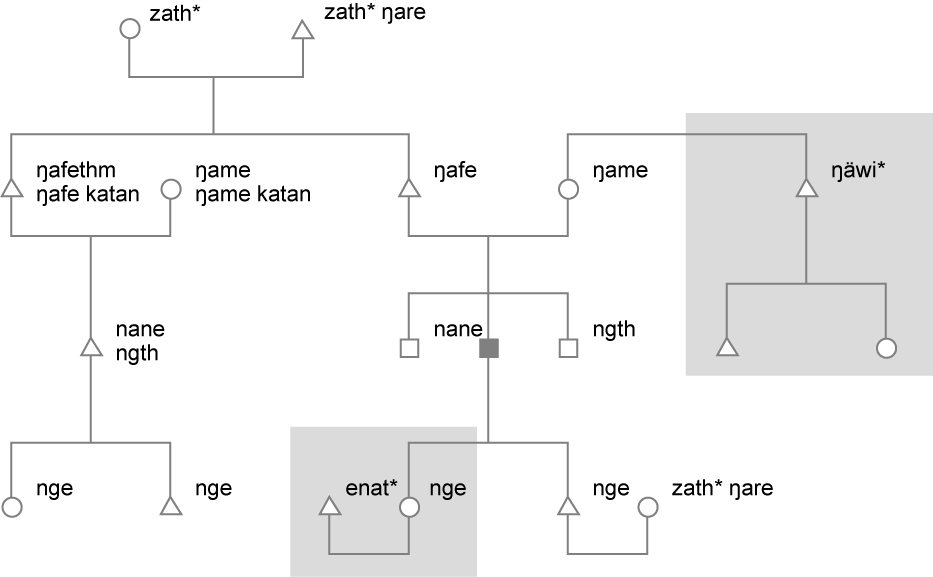
\includegraphics[width=12cm]{figures/kinship1.png}
	\caption[Consanguineal or co-resident kin terms]{Consanguineal or co-resident kin terms}
	\label{fig:kinship1}
\end{figure}%cosanguineal

The spouses of ego's children are called \emph{enat} `son in-law' and \emph{zath ŋare} `daughter in-law'. Both words are used reciprocally, i.e. they mean `parents-in-law' from the opposite perspective. The sex of the referent can be specified by adding \emph{ŋare}. Ayres points out that grandparents and grandchildren are equated by the same word \emph{zath}, which also means `moon' and `month', and as we have just seen `daughter in-law'. However, \emph{zath} is somewhat archaic, and the \ili{Nama} loan \emph{aki} with the same set of meanings is used in its place. Ayres explains this grouping of three meanings \textendash{} grandparents, grandchildren and daughter in-law \textendash{} by a ``structural incompleteness that is felt to be generated by the original exchange'' (\citeyear[226]{Ayres:ws}). She points out that the preferred arrangement for the daughter of an exchanged woman is to marry back to her mother's place. She concludes that the grouping of the three meanings in the same kin term encodes a cultural practise which ``assures the continuity of a man's patriline not simply through his own children, but through their children'' (\citeyear[227]{Ayres:ws}).

\begin{figure}
	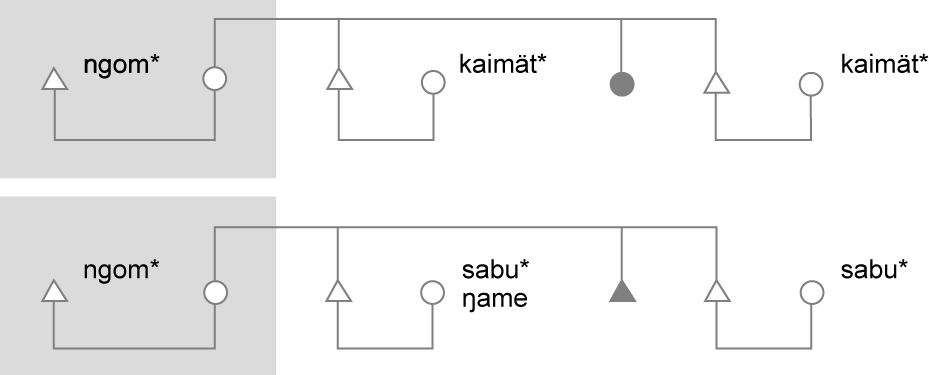
\includegraphics[width=10cm]{figures/kinship2.png}
	\caption[Same-generation, affinal kin terms for female and male ego]{Same-generation, affinal kin terms for female and male ego}
	\label{fig:kinship2}
\end{figure}%affinal

Figure \ref{fig:kinship2} shows the affinal kin terms in the same generation. The word \emph{ngom} `brother-in-law' is used by both women and men, and for men it is used reciprocally. In (\citealt[214]{Ayres:ws}), the words \emph{ntjufaré} and \emph{nakimi} [her spelling] appear in a \isi{kinship} diagram for `brother-in-law'. The former is a \ili{Kánchá} word and the latter is from Motu (\citealt[107]{Turnerlister:1935motu}). While \emph{nakimi} coexists with \emph{ngom}, \emph{ntjufare} is not used by Komnzo speakers. I suspect that this word was given to Ayres by \ili{Wára} speaking women from Yokwa. There are strong marriage ties between Rouku and Yokwa, and the process of village consolidation ({\S}\ref{modernhistory}) has led to an influx of \ili{Kánchá} speakers in Yokwa in the past. The term \emph{kaimät} is used between a woman and her brother's wife, and both are in a joking relationship. The term \emph{sabu} is used between a man and his brother's wife, and both are in a taboo relationship. The taboo is much stricter for the wife of the younger brother, who is always called \emph{sabu}. As for the wife of the older brother, one may also use \emph{ŋame} `mother' if she is sufficiently older, and the taboo relation is somewhat lax.

After a consummated exchange marriage, a special set of terms is used. These are shown in Figure \ref{fig:kinship3}. The word \emph{fäms} `exchange fellow' is used between the two men who have exchanged sisters, and the exchanged woman is called \emph{fäms ŋare} `exchange woman'. The children of the exchange couple are called \emph{fäŋame} or \emph{fäŋafe} depending on their sex. These two words are archaic in Komnzo and instead \emph{bäiŋame} or \emph{bäiŋafe} are used. The last vowel of both is sometimes dropped resulting in \emph{bäiŋam} or \emph{bäiŋaf}. These words are used reciprocally, but the last part (\emph{-ŋaf} and \emph{-ŋam}) encodes the sex of the referent. It is unclear when and how the first part changed from \emph{fä-} to \emph{bäi-}, but the consonants /ɸ/ and /{ᵐ}b/ stand in a paragidmatic relationship, because there is no voiceless counterpart of the prenasalised /{ᵐ}b/. For this reason, I suspect that the first part is a contraction of \emph{fäms}, and \emph{fäŋame} or \emph{fäŋafe} used to be \emph{fäms ŋame} `exchange mother' and \emph{fäms ŋafe} `exchange father'. Note that the same figure can be drawn for a female ego. We would only have to change the words for wife and husband, which are \emph{fzenz} and \emph{fis} respectively.

\begin{figure}
	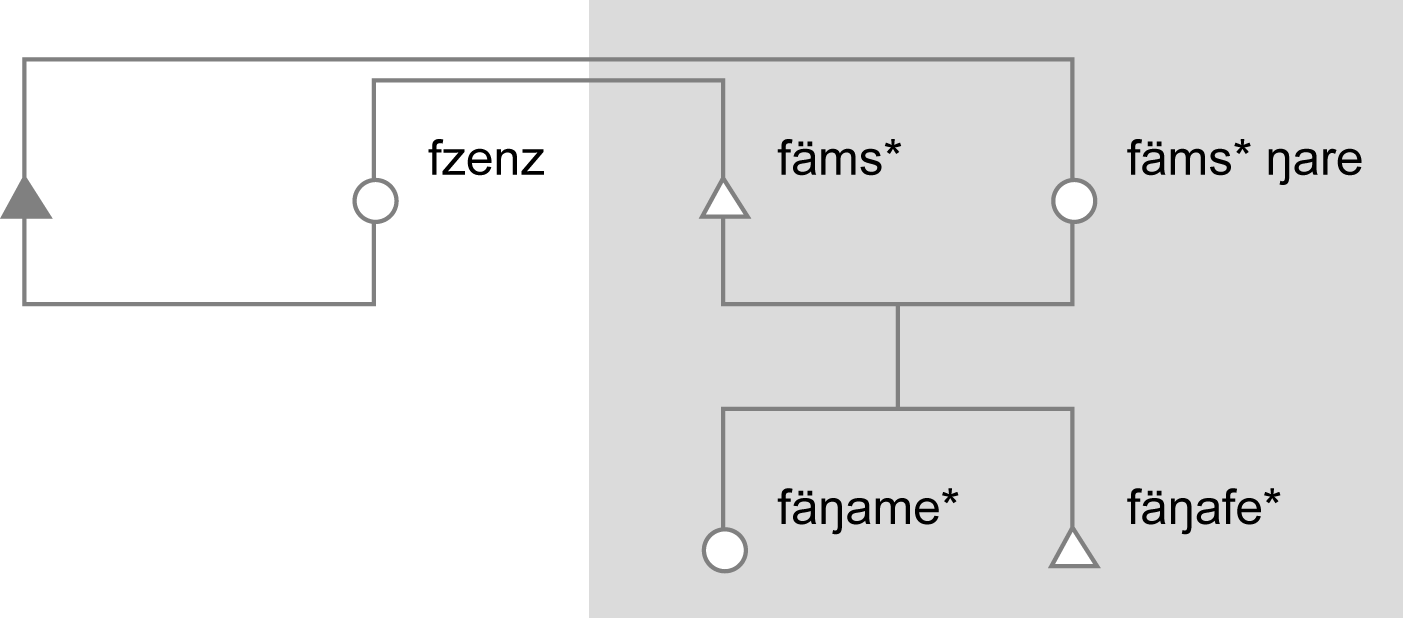
\includegraphics[width=8.5cm]{figures/kinship3.png}
	\caption[Sister-exchange kin terms: \emph{fäms}]{Sister-exchange kin terms: \emph{fäms}}
	\label{fig:kinship3}
\end{figure}%fäms

An exchange marriage also affects the children's generation. Ayres points out that cross-cousins are preferred marriage partners (\citeyear[217]{Ayres:ws}), but this excludes the children of an exchange. Cross-cousins from an exchange marriage refer to each other with the term \emph{yamit}. The relationship between them is more like that between siblings, which is corroborated by the fact that ego employs the same kin term \emph{ngom} for the husband of the \emph{yamit}. The wife of ego's \emph{yamit} is called \emph{yumad}. This is shown in Figure \ref{fig:kinship4}.

\begin{figure}
	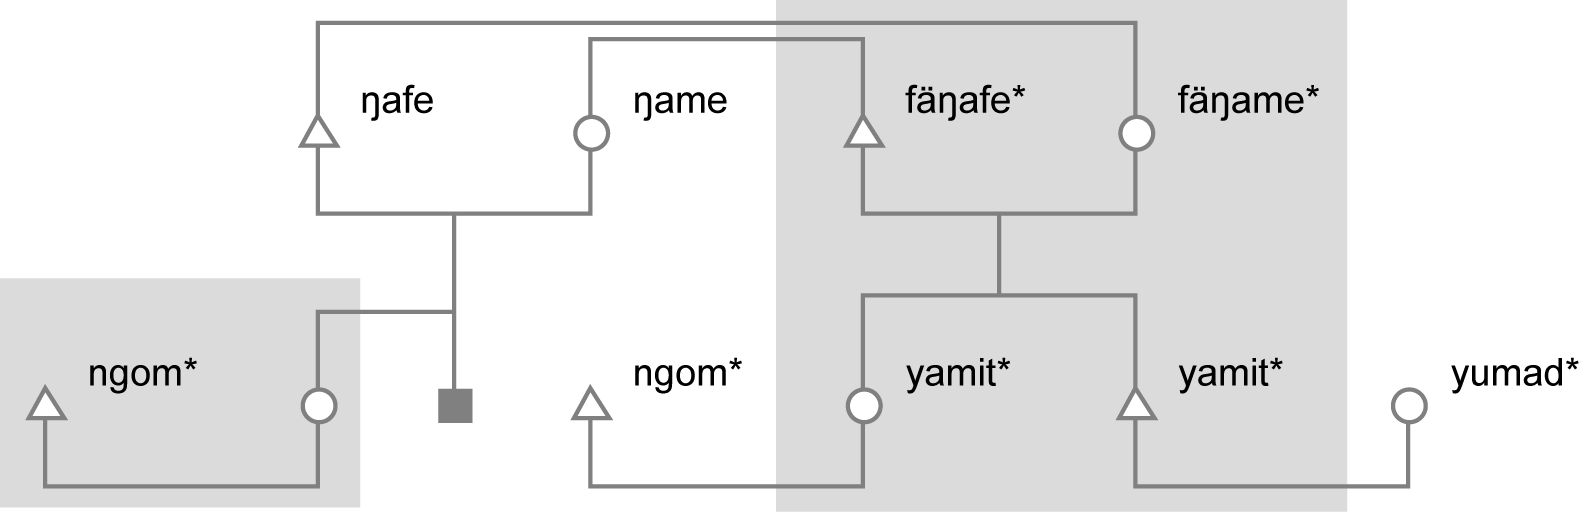
\includegraphics[width=12cm]{figures/kinship4.png}
	\caption[Sister-exchange kin terms: \emph{yamit}]{Sister-exchange kin terms: \emph{yamit}}
	\label{fig:kinship4}
\end{figure}%yamit

There is another special relation that holds between the affines and children of two sisters. Two men who are married to sisters refer to each other with the term \emph{nakum}. The parallel-cousins in such an arrangement refer to each other as \emph{naku}, and what holds for the \emph{yamit} relation is also true for the \emph{naku} relation. This is shown in Figure \ref{fig:kinship5}.

\begin{figure}
	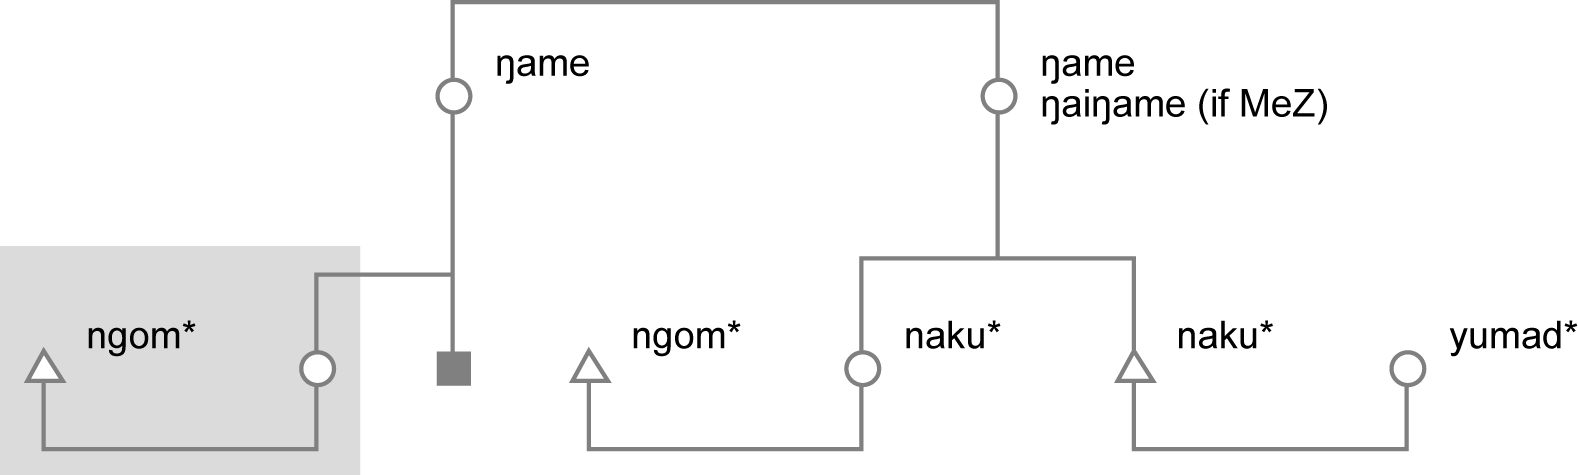
\includegraphics[width=12cm]{figures/kinship5.png}
	\caption[The \emph{naku} relationship]{The \emph{naku} relationship}
	\label{fig:kinship5}
\end{figure}%naku

The rules and regulations are often explained in terms of space and Mary Ayres focusses on this aspect in her thesis. For example, informants would often explain that two individuals cannot marry because ``they come from the same place'', meaning that their mothers come from the same place in the case of a \emph{naku} relationship. But it can also mean that they result from a direct exchange between places in the case of a \emph{yamit} relationship.

There are other terms which function similarly to kin terms. One such example is the word \emph{ngath}, which I translate as `mate'. Two children who were born around the same time are considered to be like close relatives, even if they belong to different clans and/or sections. They will grow up as close mates and they will support each other. It is up to the parents to decide who will become \emph{ngath}, but it is always children of the same sex. I know of two cases where the \emph{ngath} relationship was inherited from the fathers who were also \emph{ngath} to each other. Another example is the word \emph{ngemäku}, which is used between the biological parents of a child and the ones who have adopted the child. Adoption is very common and it occurs shortly after the weaning period. The word \emph{ngemäku} contains the word \emph{nge} `child', but the second part \emph{mäku} has no meaning by itself. A third example is the word \emph{nzäthe} `namesake'. Children are given many names when they are born. As a consequence an individual has multiple namesake relationships.

This section is closed with a comprehensive list of kin terms in \tabref{kintermstable}. Alternative terms and applications as well as comments are given in the rightmost column.

\renewcommand{\tabcolsep}{2,3pt}
\begin{table}
\caption{Summary of kin terms and other relation terms}
\label{kintermstable}
	\begin{tabularx}{\textwidth}{llp{3cm}Q}
		\lsptoprule
			{Komnzo} & {gloss}&{relation}\super{a} & comment\\\midrule
			\emph{ŋafe} & father & F, FB & also \emph{afa} (\ili{Nama} loan)\\
			\emph{ŋame} & mother & M, MZ, FBW & also \emph{ama} (\ili{Nama} loan)\\
			\emph{nane} & brother, sister & eB, eZ & FBS and FBD (if older)\\
			\emph{ngth} & brother, sister & yB, yZ & FBS and FBD (if younger)\\
			\emph{zath} & grandparent,&FF, FM, MF, MM, & also \emph{aki} (\ili{Nama} loan),\\
			&grandchild,&SS, SD, DS, DD, &used reciprocally (rcpl.), \\
			&parent-in-law,&HF, HM, SW, BSW, &can be specified for sex\\
			&daughter in-law&SSW &by adding \emph{ŋare}\\
			\emph{kaimät} & sister-in-law & BW, HZ & female perspective, used rcpl.\\
			\emph{sabu} & sister-in-law & BW, HB & male perspective, used rcpl.\\
			\emph{ngom} & brother-in-law\super{b} & ZH, WB & also for husbands of cross-cousins\super{b}, i.e. \emph{yamit's} husband, used rcpl.\\
			\emph{yumad} & n/a & n/a & wife of parallel-cousin\super{b} (\emph{yamit's} wife), used rcpl.\\
			\emph{enat} &parent-in-law& DS, WF, WM&used rcpl.\\
			&son in-law&&\\
			\emph{ŋäwi} & uncle,& MB, ZS, ZD	& also \emph{babai}, used rcpl.\\
			&niece, nephew&&\\
			\emph{fäms} & exchange\super{b}	& ZH, BW & can be specified for sex by adding \emph{ŋare}, used rcpl.\\
			\emph{fäŋame} & aunt, niece\super{b} & FZ, BD&also \emph{bäiŋam}, used rcpl.\\
			\emph{fäŋafe} & uncle, nephew\super{b} & MB, ZS&also \emph{bäiŋaf}, used rcpl.\\
			\emph{yamit} & cross-cousin\super{b} & MBS, MBD, FZS, FZD & used rcpl.\\
			\emph{naku} & parallel-cousin & MZS, MZD & used rcpl.\\
			\emph{nakum} & n/a & WZH & used rcpl.\\\midrule
			\emph{thuft} & in-law & n/a & also \emph{nakimi} (Motu loan), used rcpl.\\
			\emph{ngath} & mate & n/a & between two (predetermined) mates of the same sex, used rcpl.\\
			\emph{ngemäku} & n/a & n/a & between true parent and adopted parent, used rcpl.\\
			\emph{nzäthe} & namesake & n/a & between two people with the same name, used rcpl.\\
		\lspbottomrule
			\multicolumn{4}{l}{{\footnotesize \super{a}F=father, M=mother, B=brother, Z=sister, S=son, D=daughter, H=husband, W=wife}}\\
			\multicolumn{4}{l}{{\footnotesize \super{b}only after a consummated sister exchange marriage}}\\
	\end{tabularx}
\end{table}%kin terms

\subsection{Person reference and name avoidance}\label{personref}

There is some diversity in person referring expressions in Komnzo. In the case of \isi{name avoidance}, these may be restricted to only a subset. The common expressions ar full names (given name + family name), personal names, nicknames, kin terms, other relation terms, reference via circumspection, and the \isi{recognitional} \isi{demonstrative}.

The \isi{kinship} system as presented above lays out a number of rules of behaviour. Amongt them is a practise of \isi{name avoidance} which holds between all affines. When recording genealogies, informants would often hestitate or refuse to utter the name of a particular person and instead ask some bystander or a child to pronounce the personal name for me. Name avoidance is seen as a way of showing respect. This was explained to me by my sister while transcribing a text in which she used the personal name of her sister-in-law. When I asked her, why she had not used the appropriate kin term \emph{kaimät}, she replied that she was very angry with her at the time and showed her anger by using the personal name. Name avoidance impacts on the reference to other persons with the same personal name, to whom the speaker may not be in a name-avoidance relationship. In other words, \isi{name avoidance} is independent of the referent in a particular situation. Instead \isi{name avoidance} targets the personal name. This does not result in any practical problems because people have multiple names.

There are different solutions to ensure that the hearer understands who is meant. In addition to the appropriate kin term, one may use circumspection or a \isi{recognitional} \isi{demonstrative}. For example, the name of one of my brothers in-law is \emph{Kurai}. I should not utter his name, but use the kin term \emph{ngom} instead. In many situations, this term is sufficient to establish the correct reference. Alternatively, I can use circumspection strategy like \emph{tokoafis} `Toko's husband' or a teknonym \emph{weweaŋafe} `Wewe's father'. For teknonyms, it is usually the name of first-born child that is used, regardless of sex. A third solution is to use the \isi{recognitional} \isi{demonstrative}. The \isi{recognitional} \isi{demonstrative} can be roughly translated into English as `the one that we both know about' (\S\ref{recognitional-pronoun-subsec}).

The different strategies of \isi{person reference} can be ranked according to how much knowledge is presupposed on the part of the hearer. For example, a personal name requires very little contextual knowledge, whereas a \isi{recognitional} \isi{demonstrative} requires much more. We may rank these strategies like this: full name (\emph{Kurai Tawth}) > personal name (\emph{Kurai}) > circumspection/teknonym (\emph{tokoafis} `Toko's husband') > kin term (\emph{ngom} `brother-in-law') > \isi{recognitional} (\emph{baf} `that one'). Note that using a full name is a recent adaptation to western culture, which is only employed in the context of a census or other administrative matters. It is a common practise in PNG to use the name of the father as family name. Hence, \emph{Kurai's} father was \emph{Tawth} and therefore his full name is \emph{Kurai Tawth}. In daily interaction, this strategy is absent.

A person has a multitude of personal names or nicknames. Almost everyone has a set of five to ten names and the frequency of use of any one of these may come and go like a fashion. Shortly after birth, or sometimes even before birth, different relatives will propose names for the new-born. These may be their own names, which establishes a namesake relationship. In fact, the word \emph{nzäthe} `namesake' is the most frequent term of address. There is a special ceremony a couple of months after birth, where the name-giver presents gifts to his namesake and holds the baby for the first time. Names may also be created on the spot, as nicknames or as self-attributions. For example, the three elders of the \emph{Mrzar Mayawa} clan in Rouku are \emph{Marua}, \emph{Kaumb} and \emph{Abia}. Their respective nicknames are \emph{oroman loŋ} `old man long' because he prefers wearing long trousers, \emph{afa kwanz} `father bald head' because he is bald and \emph{afa thwä} `father catfish' because he has a big belly. The first of them, \emph{Marua}, decided one day that he should be called \emph{oroman zulai} `old man July'. To my bewilderment, I found that everyone had accepted this name within a few weeks. Interestingly, a namesake relationship may transfer all of these names to the namesake. For example, a small baby boy was given the name \emph{Marua}, thus establishing a namesake relationship. Today, the toddler is sometimes called \emph{Marua}, \emph{loŋ} or \emph{zulai}.

\subsection{Language ideology and multilingualism}\label{ideomulti}

Language ideology is characterised by a set of beliefs on the part of speakers about the role which language plays in constructing their social world (\citealt{Silverstein:1979li}, \citealt{Rumsey:1990vb} and \citealt{Makihara:2007co}). In the Morehead Region, people draw a strong connection between land and speech variety. This native linguistic ideology is similar to Aboriginal cultures, especially in Arnhem Land (\citealt{Merlan:1981ue}) and Cape York (\citealt{Sutton1978:ws}). As for the Farem people, this ideology surfaces through open statements and explanations, the expected behaviour of in-marrying women, ancestor stories, but it is also entailed in metaphors. I will briefly note some of my own observations on \isi{language ideology} here.

In Rouku, there is strong social pressure on all members of the community to speak Komnzo. This is openly expressed during public speeches, but also by individuals in conversation or during interviews. One often hears that women should not talk in ``their language'' to the children, but in Komnzo. In practice, this is often violated and virtually everybody grows up in a \isi{multilingual} context. We can take an example which is the result of the process of village consolidation described in \S\ref{modernhistory}. A number of older men originally from Rouku have stayed for a long time in \ili{Anta} or \ili{Wára}-speaking villages, and consequently their children grew up with those varieties as their main language. The children, now in their late 1940s, have moved back to Rouku. Some of them have married a woman from their natal villages and hence the dominant language of some Farem households is \ili{Anta} or \ili{Wára}. However, when I administered a socio-linguistic questionaire, they would deny speaking anything but Komnzo.

In an attempt to understand the situation, I conducted sociolinguistic interviews with about 40 people. Some of the questions targeted \isi{language ideology} (``What is your language?'', ``What do think about language mixing in the village?'', ``What language do you want your children to learn?''). The conclusion from these interviews is that language and land form an inseparable bond. I defer the statistical analysis of the interviews to another point in time. The bond between language and land is identical to the bond between a group of people and their origin place. This bond is transmitted through the father's line. An example taken from the interviews is that of an older woman who lives in Rouku. She explained to me that she grew up in Yokwa, and consequently she speaks \ili{Wára} most of the time. Although she speaks mostly \ili{Wára}, she knows that this is not the language of the place. She wishes for her children to speak Komnzo. When asked about her language she answered \ili{Kánchá} instead of \ili{Wára}. She explained that her father had moved as a teenager from a \ili{Kánchá}-speaking village to Yokwa. It follows that regardless of whether an individual uses predominantly mother's language or the language of the village, he or she will identify with the language of his or her father's place.

Mixing or shifting languages, although very common, is almost universally looked down upon. The answers as to why this behaviour is thought of as inappropriate often follow along the lines of matching language to place (``They should not speak \ili{Wára} here because this is the language of Yokwa'', ``We should not mix languages because the children will not be able to name the places and animals that belong to our land'').

Women who marry in are expected to shift to the local language, but this is often not followed because there are enough women from any one village to form small exclaves, for example of \ili{Wára}-speaking women in Komnzo-speaking territory. It is hard to corroborate, but informants say this was enforced more in the past. For example, there are spells and rituals to enhance the language learning process on the side of the woman. One ritual involves splitting a thin bamboo behind a woman's head and whispering a spell. This procedure is said to facilitate the learning process. I asked many times to have this procedure performed on me, but people refused to do it because I would forget my native \ili{German}. There are other customs and rules which connect land and language. For example, it is forbidden to talk another language at story places and men would introduce their new bride to a \textit{menz} `story man' at a particular place in order to avoid sickness. The policy of language shift expected from women is hardly ever enforced these days and one might wonder whether it ever was. Ayres (\citeyear[226]{Ayres:ws}) describes the preference for a daughter to marry back into her mother's village, which she calls a short marriage cycle. This pattern establishes strong ties between particular villages. In the case of the Rouku it is the village of Yokwa and the language is \ili{Wára}. As mentioned above, groups of women from Yokwa would often speak \ili{Wára} between themselves or to their children and there is no reason why this should have been different in the past. But when asked about this, they would look down on `language mixing' and stress the importance of the correct language at the right place.

Ancestor stories almost always involve comments on language. For example, the Kuramonggo myth which is found across the Morehead Region involves an ancestor who heard voices coming from a tree. Different versions are found in (\citealt[299]{Williams:1936transfly}) and (\citealt[102]{Ayres:ws}). In the myth, the ancestor starts to chop the tree into segments from the top to the bottom. With each little bit that he chopped, people speaking different languages came out and started running towards their respective places. The further he worked his way to the bottom of the tree, the more intelligible the words became to him. When he reached the base of the tree, he heard his own language and thus his own people emerged from the tree. A common \isi{metaphor} that explains the language situation from a local perspective builds on this story. One often hears the local language being described as \emph{zfth} `base of a tree' and all the surrounding languages as \emph{tuti} `branches'. The tree \isi{metaphor} is important in the local perspective. For example, women are jokingly described as \textit{bidr} `flying foxes' because they fly from tree to tree, and sometimes they are described as \textit{fätü} `a wild yam' or \textit{saka} `mustard vine' because the vines of these plants grow on trees.

\section{Komnzo within the Yam languages}\label{Komnzowithinyam}

This section situates Komnzo within the \ili{Yam languages}. This language family was formerly referred to as the ``Morehead and Upper Maro Rivers languages'', or ``\ili{Morehead-Maro} languages'' (\citealt{Wurm:1971uw}). This name is misleading because its geographical boundary in the east, the Morehead River, excludes all the languages of the \ili{Nambu} subgroup. I follow Evans in using the more precise term ``\ili{Yam languages}'' (\citeyear[124]{Evans:2012wp}). Not only are yams the staple food, and of high cultural importance in exchange feasts, they also gave rise to the \isi{senary} \isi{numeral system}, which is unique to the languages of the family. In addition to the \ili{English} word yam [jæm], there is a lexemes \emph{yam} [jam] in many of the \ili{Yam languages}, which carries high cultural significance. For example, in Komnzo it means `footprint, custom, tradition' and in \ili{Nen} it means `law, tradition, culture'.

The \ili{Yam languages} comprise three subgroups: \ili{Nambu} in the east, \ili{Tonda} in the west, and Yei, which has only a single member. A first attempt to reconstruct various aspects of the proto language can be found in (\citealt{Evans:sng}). While it is relatively easy to place Komnzo in the \ili{Tonda} subgroup, it is much harder to classify the units within \ili{Tonda}; in other words to draw a boundary between language and dialect. Are Komnzo, \ili{Anta} and Wérè dialects of \ili{Wára} as Ethnologue\footnote{\url{http://www.ethnologue.com/language/tci}} portrays it or are they languages in their own right? Peter Mühlhäusler (\citeyear{Muhlhausler:2006naming}) points out the difficulty and futility in answering such questions in Papua New Guinea and the contradictions that different researchers have produced in the past. As the preceding description of \isi{language ideology} has highlighted, these are considered to be different languages from a local perspective. I remain agnostic throughout this section and offer a short conclusion at the end.

I discuss sound correspondences and sound changes first. Next, I show some lexicostatistic data from (\citealt{Wurm:1971uw}) and (\citealt{Clifton:1991fly}). Last, I discuss case markers, pronouns and verb morphology. I include here the following \ili{Tonda} varieties: Komnzo, \ili{Anta}, \ili{Wára}, \ili{Wèré}, \ili{Ránmo}, \ili{Blafe}, \ili{Wartha} Thuntai and \ili{Kánchá}. I refer the reader to Figure \ref{fig-01-SNGmap} for an overview of where these varieties are spoken. I do not include \ili{Arammba}, which I take to be sufficiently different to be considered a separate language (\citealt{Bouve:2003ar}). I have no data for the \ili{Tonda} varieties spoken on the Indonesian side of the border (Baedi, \ili{Ngkolmpu}, Smerky, Bakari, Taemer and Sota), and only very little data on \ili{Kémä}.

With the exception of Komnzo, the spelling of the names of these varieties is adopted from Ethnologue, which in turn goes back to an \isi{orthography} workshop held by SIL missionaries in Morehead in 2000. Note that the orthographies were developed for each variety with the result that the graphemes in the language names have different phonetic values: Komnzo [kɞ̆mⁿdʒo], \ili{Anta} [aⁿda], \ili{Wára} [wæra], \ili{Wèré} [wɞ̆rɛ], \ili{Ránmo} [rænmo], \ili{Blafe} [ᵐblæɸe], \ili{Wartha} Thuntai [warða ðuⁿda͡ı], \ili{Kánchá} [kə̆ⁿdza]. To ensure comparability in this section, I will employ IPA for all language examples, including Komnzo.

\subsection{Phonology}\label{comp-phon}

First, I will turn to phonological correspondences. In this section, the languages in the tables have been sorted geographically: west (left) to east (right). We find that only \ili{Blafe} and \ili{Ránmo} have an /l/ phoneme in their respective inventories. \tabref{lth} shows that this phoneme corresponds to an interdental fricative in Komnzo, \ili{Anta}, \ili{Wára}, \ili{Wèré}, \ili{Wartha} Thuntai and \ili{Kánchá}. Note that final \isi{devoicing} produces [θ] in coda position.

\begin{table}
\caption{Correspondence set: [l] versus [ð]}
\label{lth}
\fittable{
	\begin{tabular}{llllllll}
		\lsptoprule
			&{item} &Blafe, Ránmo &Wartha &Kánchá &Wèré &Anta &Komnzo, Wára \\\midrule
			1 &{tongue} &læmin &ðæmin &ðæmin &ðæmin &ðæmin &ðæmin\\
			2 &{faeces} &wəl &wəθ &wəθ &wəθ &wəθ &wəθ\\
			3 &{wet} &kilkil &kiθkiθ &tʃiθtʃiθ &tiθtiθ &tiθtiθ &tʃiθtʃiθ\\
			4 &{armpit} & {\ᵑ}gəlki &{\ᵑ}gəθki &kəθtʃi &{\ᵑ}gəθki &{\ᵑ}gəθtʃi &{\ᵑ}gəθtʃi\\
		\lspbottomrule
	\end{tabular}
	}
\end{table}%Correspondence set: [l] versus [ð]

A second set shows the correspondence of bilabial stops, [ᵐb] and [b], in \ili{Blafe}, \ili{Ránmo} and \ili{Wartha} Thuntai to lavio-\isi{velar} stops, [{\ᵑ}gʷ] and [kʷ], in Komnzo, \ili{Anta}, \ili{Wára}, \ili{Wèré} and \ili{Kánchá} in \tabref{mbng}. We find that the labial part is sometimes realised as a rounded back vowel, [{\ᵑ}go] and [ko], in \ili{Kánchá}, \ili{Wèré} and \ili{Wartha} Thuntai, for example in lines 3 (`butterfly') and 4 (`crow'). One possible explanation is a process of develarisation that has occurred in \ili{Blafe}, \ili{Ránmo} and \ili{Wartha} Thuntai.

\begin{table}
\caption{Correspondence set: [ᵐb/b] versus [{\ᵑ}gʷ/kʷ]}
\label{mbng}
\fittable{
	\begin{tabular}{l llllll}
		\lsptoprule
			&{item} &Blafe, Ránmo & Wartha & Kánchá& Wèré &Komnzo, Wára, Anta\\\midrule
			1 &{nest} &ᵐbəl &ᵐbəθ &{\ᵑ}gʷəθ	&{\ᵑ}gʷəθ &{\ᵑ}gʷəθ\\
			2 &{mosquito} &ᵐbæ &ᵐbæ &{\ᵑ}gʷæ &{\ᵑ}gʷæ &{\ᵑ}gʷæ\\
			3 &{butterfly} &taᵐbam &taᵐburam &ᵐbæ{\ᵑ}goram &\multicolumn{2}{c}{ᵐbæ{\ᵑ}gʷərəm}\\
			4 &{crow} &ᵐbaθ &kot &koθ &koθ &kʷaθ\\
			5 &{light} &praja &bæjan &kʷajan &kʷajan &kʷajan\\
			6 &{sick} &bik &bik &kʷik &kʷik &kʷik\\
		\lspbottomrule
	\end{tabular}
	}
\end{table}%Correspondence set: [ᵐb/b] versus [{\ᵑ}gʷ/kʷ]

There is a small set of words in which the bilabial fricative corresponds to a prenasalised bilabial stop. The set in \tabref{fmb} once again groups \ili{Blafe}, \ili{Ránmo} and \ili{Wartha} Thuntai against Komnzo, \ili{Anta}, \ili{Wára}, \ili{Wèré} and \ili{Kánchá}. Interestingly, the form of the \Second\Sg.{\Abs} `you' groups \ili{Blafe}, \ili{Ránmo}, \ili{Wartha} Thuntai, \ili{Kánchá} and Komnzo together.

\begin{table}
\caption{Correspondence set: [ᵐb] versus [ɸ]}
\label{fmb}
\fittable{
	\begin{tabular}{lllllll}
		\lsptoprule
			&{item}& Blafe, Ránmo & Wartha &Kánchá, Komnzo & Wára, Anta, Wèré\\
			\midrule
			1 &{wife} &ᵐbə{\ᵑ}geⁿt &ᵐbə{\ᵑ}geⁿts &ɸətʃeⁿts &ɸətʃeⁿts\\
			2&{husband} &ᵐbi &ᵐbi &ɸis &ɸis\\
			3&\Second\Sg.{\Abs} `you' &ᵐbæ &ᵐbæ &ᵐbæ &ɸe\\
		\lspbottomrule
	\end{tabular}
	}
\end{table}%Correspondence set: [ᵐb] versus [ɸ]

A clear \isi{directional} change is palatalisation before front vowels. In \tabref{palatal}, I show only a subset of the varieties. Komnzo represents those in which palatalisation has occured. This also holds true for \ili{Anta} and \ili{Wára}, but the forms are slightly different. \ili{Wartha} Thuntai represents those in which palatalisation has not occured. This is also the case for \ili{Blafe} and \ili{Ránmo}. The table shows that \ili{Wèré} and \ili{Kánchá} are somewhat irregular. In lines 4 and 5 (`house' and `one') palatalisation occurs in \ili{Wèré}, but not in \ili{Kánchá}. Line 6 (`armpit') shows the opposite. In lines 1-3 (`woman', `I', `people') palatalisation has occured in both and in line 7 (`tree') in neither. I have included \ili{Nama}, a \ili{Nambu} language, to show that \ili{Nambu} languages have preserved the original \isi{velar} quality, for example in lines 1, 3, and 4 (`woman', `people', `house'). Note that in line 5 (`one'), \ili{Nambu} has dropped the first consonant. The deletion of initial \isi{velar} \isi{nasals} is a regular change in \ili{Nambu} languages; for example, `mother' is [ŋame] in Komnzo, but [ama] in \ili{Nama} and \ili{Nen}. Note that the conditioning context for palatalisation has been lost in line 4 (`house'), because the examples end in a consonant. \ili{Nama} attests a vowel in this position.

\begin{table}
\caption{Palatalisation before front vowels}
\label{palatal}
	\begin{tabularx}{\textwidth}{llXXXXX}
		\lsptoprule
			&{item} & Wartha	&Kánchá &Wèré &Komnzo &Nama\\\midrule
			1 &{woman}\super{a} &ᵐbroki &ᵐbrotʃi &ᵐbrasi &ᵐbratʃi &ᵐbrake\\
			2 &\Fsg.\Abs &{\ᵑ}ga &ⁿdʒæ &se &ⁿdʒæ &(jəⁿd)\\
			3 &{people}\super{b} &{\ᵑ}gʏⁿtəm &tʃœⁿtəm &sœⁿtmæ &tʃœⁿtmæ &{\ᵑ}gʏⁿtmæ\\
			4 &{house} &meⁿk &mə{\ᵑ}k &məⁿts &məⁿts &mæ{\ᵑ}go\\
			5 &1 ({one}) &ŋæᵐbi &ŋæᵐbi &næᵐbi &næᵐbi &æᵐbiro\\
			6 &{armpit} &{\ᵑ}gəθki &kəθtʃi &{\ᵑ}gəθki &{\ᵑ}gəθtʃi &-\\
			7 &{tree species} &{\ᵑ}gœⁿt &{\ᵑ}gœⁿt &{\ᵑ}goⁿt &ⁿdʒœⁿts &-\\
		\lspbottomrule
		\multicolumn{7}{l}{\footnotesize \super{a}a woman in the time after giving birth}\\
		\multicolumn{7}{l}{\footnotesize \super{b}people who live to the west of one's own group}\\		 
	\end{tabularx}
\end{table}%Palatalisation before front vowels

The last set shows the correspondence between stops and affricates. In \tabref{affrstop}, \ili{Blafe}, \ili{Ránmo}, \ili{Wèré} and \ili{Anta} are grouped against Komnzo, \ili{Wára}, \ili{Wartha} Thuntai and \ili{Kánchá}.

\begin{table}
\caption{Correspondence set: stop versus affricate}
\label{affrstop}
	\begin{tabularx}{\textwidth}{llXXXXXX}
		\lsptoprule
			&{item} &Blafe, Ránmo &Wartha &Kánchá &Wèré &Anta &Komnzo, Wára\\\midrule
			1 &{pain} &ti &ⁿdʒi &tʃi &ti &ti &tʃi\\
			2 &{right} &tawe &tsowe &tsowe &tawe &tawe &tsawe\\
			3 &{bowerbird} &ⁿdojar &ⁿdʒojar &ⁿdʒojar &ⁿdʒojar &ⁿdojar &ⁿdʒœjar\\
		\lspbottomrule
	\end{tabularx}
\end{table}%Correspondence set: stop versus affricate

Concluding the comparison of phonological correspondences, we find that Komnzo and \ili{Wára} are almost always grouped together, and we may include \ili{Anta} as well. \ili{Kánchá} and \ili{Wèré} share a number of correspondences with Komnzo, \ili{Wára} and \ili{Anta}, but they differ in some sets. \ili{Blafe}, \ili{Ránmo} and \ili{Wartha} Thuntai are different in almost all sets. While \ili{Blafe} and \ili{Ránmo} are always grouped together, \ili{Wartha} Thuntai can be grouped with the other varieties in some sets.

\subsection{Lexicon}\label{comp-lex}

In this section, I will present data from (\citealt{Wurm:1971uw}) and (\citealt{Clifton:1991fly}). I defer the statistical analysis of my own wordlists to a latter point in time.

A first calculation of cognate rates was offered by Wurm. His dataset comprised \ili{Tonda} and \ili{Nambu} languages as well as and Yei and \ili{Marori}. In \tabref{wurm1971} only the \ili{Tonda} varieties have been extracted. Wurm's language labels refer to different \ili{Tonda} varieties: Upper Morehead (Komnzo, \ili{Wára}, \ili{Anta}, \ili{Arammba}), Lower Morehead (\ili{Kánchá}), \ili{Tonda} (\ili{Blafe}, \ili{Ránmo}, \ili{Wartha} Thuntai, \ili{Wèré}) and \ili{Kanum} (Baedi, \ili{Ngkolmpu}, Smerky, Bakari, Taemer, Sota).

\begin{table}
\caption[Cognate rates]{Cognate rates (adopted from \citealt[159]{Wurm:1971uw})}
\label{wurm1971}
	\begin{tabularx}{.47\textwidth}{|c|c|c|c|}
		\cline{1-1}
		Upper Mhd&\multicolumn{3}{c}{}\\\cline{1-2}
		71\%&Lower Mhd&\multicolumn{2}{c}{}\\\cline{1-3}
		60\%&55\%&\ili{Tonda}&\multicolumn{1}{c}{}\\\cline{1-4}
		39\%&39\%&40\%&\ili{Kanum}\\\cline{1-4}
	\end{tabularx}
\end{table}%Wurm cognates

A more fine-grained dataset comes from a SIL survey conducted by Clifton, Dyall and O'Rear (\citeyear{Clifton:1991fly}), who collected wordlists in 18 villages of both \ili{Tonda} and \ili{Nambu} languages. In \tabref{clifton1991}, I will only show the \ili{Tonda} varieties, but I exclude \ili{Arammba}, Rema and \ili{Kémä}, and I choose Bondobol as the village representative of \ili{Kánchá}. Moreover, I have rearranged their data in order to present the varieties geographically from west to east.

\begin{table}
\caption[Rates of shared vocabulary]{Rates of shared vocabulary (extracted from \citealt{Clifton:1991fly})}
\label{clifton1991} 
	\begin{tabularx}{.7\textwidth}{|c|c|c|c|c|c|c|c|}
		\cline{1-1}
		\ili{Blafe}& \multicolumn{7}{c}{} \\ \cline{1-2}
		80\% &\ilit{Ránmo}& \multicolumn{6}{c}{} \\ \cline{1-3}
		63\% & 59\% &\ilit{Wartha}& \multicolumn{5}{c}{} \\ \cline{1-4}
		32\% & 40\% & 52\% &\ilit{Kánchá}& \multicolumn{4}{c}{} \\ \cline{1-5}
		49\% & 55\% & 55\% & 59\%&\ilit{Wèré}& \multicolumn{3}{c}{} \\ \cline{1-6}
		43\% & 51\% & 50\% & 70\%& 84\%&\ilit{Wára}& \multicolumn{2}{c}{} \\ \cline{1-7}
		44\% & 51\% & 50\% & 61\%& 72\%& 82\%&\ilit{Anta}& \multicolumn{1}{c}{} \\ \cline{1-8}
		41\% & 49\% & 46\% & 70\%& 72\%& 87\%& 88\%&Komnzo\\ \cline{1-8}
	\end{tabularx}
\end{table}%O'Rear shared vocab

My own wordlists confirm the data in \tabref{clifton1991}. We can draw some conclusions: (i) \ili{Blafe} and \ili{Ránmo} can be grouped together, (ii) \ili{Wartha} Thuntai is different from all other varieties, (iii) Komnzo, \ili{Wára} and \ili{Anta} can be grouped together, (iv) \ili{Wèré} and \ili{Kánchá}, though different from each other, are close to Komnzo, \ili{Wára} and \ili{Anta}. If we compare these statements to the map in Figure \ref{fig-01-SNGmap}, we find that the rates of shared vocabulary between Komnzo, \ili{Wára}, \ili{Anta}, \ili{Wèré} and \ili{Kánchá} roughly reflect geography. As for \ili{Blafe}/\ili{Ránmo} and \ili{Wartha} Thuntai, this cannot be said. In other words, if we try to understand the relation of these varieties as a dialect chain, we would have to make two cuts. The first cut splits off \ili{Blafe} and \ili{Ránmo}. The second cut singles out \ili{Wartha} Thuntai, while the remaining varieties belong to a single dialect chain.

\subsection{Morpho-syntax}\label{comp-morph}

As an intermediate summary, we can conclude that Komnzo, \ili{Anta}, \ili{Wára}, \ili{Wèré} and \ili{Kánchá} are somewhat closer together as opposed to \ili{Blafe}, \ili{Ránmo} and \ili{Wartha} Thuntai. Therefore, I will focus on the first group in this section.

\tabref{compcase} shows a comparison of case markers. We find that Komnzo deviates from the other varieties in the ergative singular and non-singular, and in the allative. \ili{Kánchá} deviates from the others in the ablative and the locative for consonant-final words.

\begin{table}
\caption{Comparison of case markers}
\label{compcase}
	\begin{tabularx}{.8\textwidth}{XXXXXl}
		\lsptoprule
			& \ilit{Kánchá} &\ilit{Wèré} &\ilit{Wára} &\ilit{Anta} &Komnzo \\\midrule
			\Erg.\Sg&-o&-o&-o&-o&-ɸ\\
			\Erg.\Nsg&-oi&-ai&-əı&-əı&-jə\\
			\All&-ɸ&-ɸ&-ɸ&-ɸ&-ɸo\\
			\Abl&-ɸo&-ɸa&-ɸa&-ɸa&-ɸa\\
			{\Loc} V\_&-n&-n&-n&-n&-n\\
			{\Loc} C\_&-i&-en&-en&-en&-en\\
		\lspbottomrule
	\end{tabularx}
\end{table}%case markers

\tabref{comp-pron} shows a comparison of free pronouns. We find that Komnzo and \ili{Kánchá} share a number of forms or some element of a form. For example the first consonant of the first and second \isi{person} in both \isi{absolutive} and \isi{ergative} case. In the \isi{possessive} non-singular pronouns, only Komnzo and \ili{Kánchá} attest a separate element which signals \isi{non-singular} \emph{-me} in addition to the vowel change found in all varieties. However, the first consonant of the third \isi{person} \isi{ergative} and \isi{possessive} pronouns differs only in \ili{Kánchá}.

As the last topic in this section, I will briefly address the marking of \isi{dual} \isi{number}. As in most \ili{Yam languages}, \isi{dual} \isi{number} is marked on the \isi{verb}. The affix encodes \isi{dual} versus \isi{non-dual} \isi{number}, and its value has to be integrated with information from other morphological sites to yield the three \isi{number} values \isi{singular}, \isi{dual} and \isi{plural}. I address this topic in \S\ref{dualextrs} and \S\ref{number-subsec}. For now, it is sufficient to compare the site of \isi{dual} marking on the \isi{verb}. In some varieties this depends on the type of \isi{verb} stem which is employed. Most verbs have two stems which are sensitive to \isi{aspect}. While multiple \isi{verb} stems are attested in all \ili{Tonda} varieties, the encoding of duality differs. In Komnzo, \ili{Anta}, \ili{Wára} and \ili{Kánchá}, there are two options: duality is encoded in a suffix if the `\isi{extended stem}' is used, but in a prefix if the `\isi{restricted stem}' is used. The meaning of these labels in Komnzo is explained in \S\ref{roots-and-temp}. Only in \ili{Wèré}, duality is always encoded in a suffix regardless of the type of stem. \ili{Blafe}, \ili{Ránmo} and \ili{Wartha} Thuntai have lost \isi{dual} marking on both stem types. In these three varieties, \isi{dual} marking occurs only in high frequency verbs such as the copula or the verb `walk', where it is usually suppletive. I sketch out a tentative historical explanation of this in \S\ref{comparativenoteextrs}.

\begin{table}
\caption{Comparison of free pronouns}
\label{comp-pron}
	\begin{tabularx}{\textwidth}{XXXXXXl}
		\lsptoprule
			& &\ilit{Kánchá} &\ilit{Wèré} &\ilit{Wára} &\ilit{Anta} &Komnzo \\\midrule
			\multirow{4}{*}{\Abs}&\Fsg&ⁿdʒæ&se&tʃe&tʃe&ⁿdʒæ\\
			&\Fnsg&ni&ni&ni&ni&ni\\
			&\Second&ᵐbæ&ɸe&ɸe&ɸø&ᵐbæ\\
			&\Third&ɸi&ɸi&ɸi&ɸi&ɸi\\\midrule
			\multirow{6}{*}{\Erg}&\Fsg&ⁿdʒən&sən&tsən&tsən&ⁿdʒe\\
			&\Fnsg&nin&ni&ni&ni&ni\\
			&\Ssg&ᵐbən&ɸən&ɸən&ɸən&ᵐbe\\
			&\Snsg&ᵐbən&ɸe&ɸən&ɸən&ᵐbənə\\
			&\Tsg&tʃaɸ&naɸo&naɸo&naɸo&naɸ\\
			&\Tnsg&tʃaɸ&naɸ&naɸ&naɸ&naɸa\\\midrule
			\multirow{6}{*}{\Poss}&\Fsg&ⁿdzuni&ⁿdone&ⁿdzone&ⁿdone&ⁿdzon\\
			&\Fnsg&ⁿdʒenme&ⁿdane&ⁿdzane&ⁿdane&ⁿdʒenme\\
			&\Ssg&ᵐbuni&ᵐbone&ᵐbone&ᵐbone&ᵐbone\\
			&\Snsg&ᵐbenme&ᵐbane&ᵐbane&ᵐbane&ᵐbenme\\
			&\Tsg&tʃaɸani&naɸəne&naɸəne&naɸəne&naɸane\\
			&\Tnsg&tʃaɸanme&naɸane&naɸane&naɸane&naɸanme\\
		\lspbottomrule
	\end{tabularx}
\end{table}%free pronouns

\subsection{Summary}\label{comp-sum}

In conclusion, we may say that the different levels of comparision converge. Sound correspondences, lexicostatistics are well as morphological differences single out at least three separate units: \ili{Blafe}/\ili{Ránmo}, \ili{Wartha} Thuntai and a chain of dialects, which we may call `Eastern \ili{Tonda}'. The latter comprises \ili{Wèré}, \ili{Wára}, \ili{Kánchá}, \ili{Anta}, Komnzo and probably \ili{Kémä}. Eastern \ili{Tonda} shows characteristics which are typical of dialect chains: geographically distant varieties, for example Komnzo and \ili{Wèré} or \ili{Anta} and \ili{Kánchá}, show the biggest differences. Close neighbours, on the other hand, like Komnzo and \ili{Wára} or \ili{Anta} and \ili{Wèré} are very similar. That being said, I will remain cautious until more data has been gathered, and I will continue to refer to all of them as varieties. In this way, I pay respect to the native linguistic ideology which picks up on the slightest differences as being highly emblematic markers of socio-linguistic identity.

\section{Previous work and methodology}\label{prevmethod}

\subsection{Previous work}\label{previouswork}

There has been no previous research on Komnzo that goes beyond the collection of wordlists. One example is the SIL survey discussed in the preceding section (\citealt{Clifton:1991fly}). The activity of SIL missionaries in the area has led to a number of \isi{orthography} worksheets, unpublished manuscripts, surveys or theses. Examples of work on the surrounding varieties include a grammatical sketch of \ili{Arammba} (\citealt{Bouve:2003ar}), a thesis on \ili{Wára} verb morphology (\citealt{Sarsa2001:wa}) and a socio-linguistic survey of the \ili{Tonda} subgroup (\citealt{Grummit:2012sur}).\footnote{I wrote a review of the survey, which can be found under the following URL: \url{https://zenodo.org/record/1404752}}

The ethnographic perspective is much better covered in the case of Komnzo. Mary Ayres conducted research in Rouku around 1980, which culminated in her thesis on locality and exogamous group definition (\citealt{Ayres:ws}). While she states that she did acquire Komnzo during her time in the field, she did record a number of stories in Komnzo and other \ili{Yam languages}. On top of that she provides a valuable description and analysis of specific terms and concepts. The ethnography of the \ili{Keraki} people, the speakers of \ili{Nambu}, written by Williams remains the most comprehensive description of any culture in Southern New Guinea (\citealt{Williams:1936transfly}).

There has been a renewed academic interest in the region in recent years, and the present study is part of this. Nick Evans has gathered a team of scholars who work on various languages of the wider region, but also on different \ili{Yam languages}. Matthew Caroll has written a PhD thesis on \ili{Ngkolmpu}, a related language of the Tonda subgroup, with a special focus on \isi{distributed exponence} \citep{Carroll:Ngkolmpu}. Bruno Olsson has published a descriptive PhD grammar of \ili{Marind} \citep{Olsson:Marind}. Jeff Siegel has published on the morphology of tense and aspect in \ili{Nama} (\citealt{Siegel:2015bp}), the eastern neighbour of Komnzo. Wayan Arka has written on \isi{tense} and agreement in \ili{Marori}, an endangered isolate spoken on the Indonesian side of the border (\citealt{Arka:2012tt}). Nick Evans has published on many topics in \ili{Nen} such as positional verbs (\citealt{Evans:2014bz}), valency (\citealt{Evans:2015wy}), inflection (\citealt{Evans:2015to}) and quantification (\citealt{Evans:quant}). An overview of the linguistic situation of the Southern New Guinea Region has been published in (\citealt{Evans:sng}).

\subsection{This project}\label{thisproject}

This project began with a pilot fieldtrip to the Morehead district in September of 2010. At the time, my goal was to establish contact to a community that speaks one of the \ili{Tonda} languages. I did not know which village or variety I was going to work on. When I arrived in Daru, I met three members of the local level government from the Morehead district who had come for administrative work to the regional capital. The three were Augustin Bikaninis from Wando (\ili{Blafe}), Bongai Njyar from Wämnefr (\ili{Kémä}) and Abia Bai from Rouku (Komnzo). It was Abia Bai who invited me to accompany him to Rouku. I received a warm and friendly welcome to the community and I stayed for eight weeks. I explained my intentions and people agreed that I may return regularly. Abia Bai adopted me into his clan (\emph{Mrzar Mayawa}) and I was given the local name \emph{Bäi} after Abia's father.

My perspective on the culture and language of the Farem has been dominated by people of the Mayawa section. This is visible in the text corpus as most texts are from speakers who belong to this section. However, I took care that my presence and impact in the village was not limited to this group, and {\textendash} more importantly for this work {\textendash} that my description of the language be confirmed by all Farem people.

I spent a total of 16 months in Rouku: two months in 2010, six months in 2011, three months in 2012, three months in 2013 and two months in 2015. During this time, I visited villages along the Morehead highway from Wereaver in the west as far as Bimadbn in the east. I visited Mari in the south and Uparua in the north. I was not able to visit villages on the Indonesian side of the border, and I did not travel to the extreme southwest (Bula, Wando and Korombo) nor did I travel to the north (Setavi, Kiriwo) of the area.

In Rouku, I lived in the house of Abia Bai and his wife Lucy together with their children Nakre, Janet, Sukawi, Nema and Alan. The oldest children Elise and Riley had already moved out of the house. Elise married a man from Wando, far in the west. Riley lives with his wife in Rouku. In the beginning, I concentrated my work on Abia Bai who possesses a great deal of knowledge about history, mythology and the natural world. For elicitation and structural analysis I worked together with my brothers Riley Abia and Daure Kaumb. It was only during my second fieldtrip in 2011 that I discovered the interest and talent of my sister Nakre in linguistic work. She became my main informant together with her father Abia. Their complementary talents have contributed greatly to this project. Abia is not only a great story-teller, but he proved to be an unlimited resource of knowledge. Nakre is a diligent worker in the transcription and translation of recordings, and she patiently answered long lists of questions and worked through complex verb paradigms in elicitation with me.

\begin{figure}
	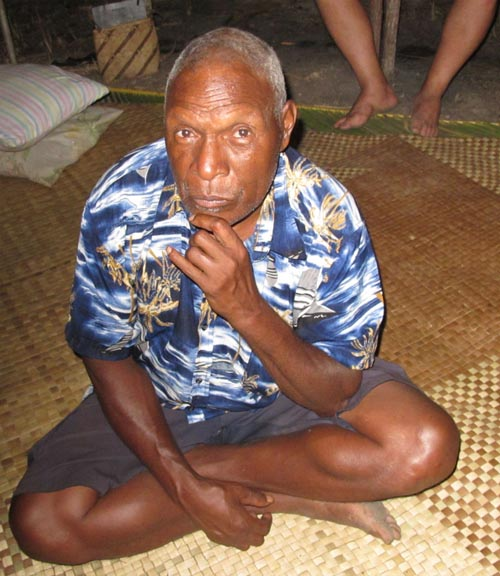
\includegraphics[width=.4\textwidth]{figures/foto-abia.jpg}
	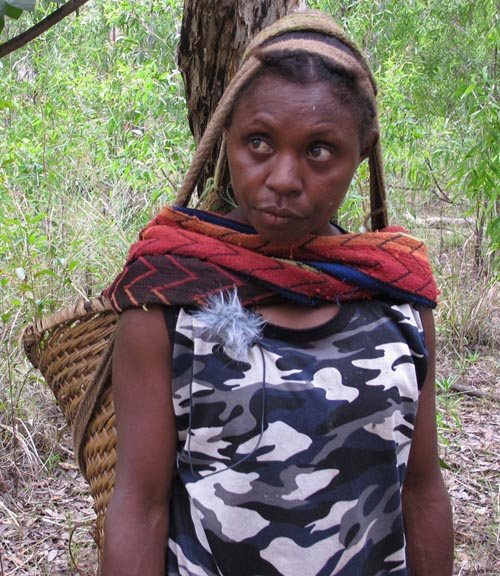
\includegraphics[width=.4\textwidth]{figures/foto-nakre.jpg}
	\caption{Abia and Nakre}
	\label{fig:abia-nakre}
\end{figure}%Abia and Nakre

From 2011 onwards, the documentation of Komnzo was funded and supported by the \textsc{dobes} project of the Volkswagen Foundation.\footnote{\textsc{dobes} stands for \ili{German} `Dokumentation bedrohter Sprachen'.} The funding covered the basic documentation of two languages, namely Komnzo and \ili{Nen}, the language of Bimadbn village, the latter of which is the language of the village Bimadbn which Nick Evans has been working on since 2008. The funding allowed us to buy a solar setup and ship it to both villages providing electricity for a computer, recording equipment and lights during the evening hours. Additionally, the \textsc{dobes} project provided financial support to bring in academics who work in the field of biology. Kipiro Damas spent one week in Rouku in 2011 and again in 2015. He collected and later identified numerous plant specimens. Chris Healey identified and photographed over 100 bird species, thereby eliciting many fascinating narratives about cultural significance of birds. Julia Colleen Miller visited Rouku on two fieldtrips conducting socio-linguistic interviews as well as creating high-quality recordings suited for phonetic analysis.

\subsection{The text corpus}\label{thetextcorpus}

The last decade has seen an exceptional increase in creating and archiving digital language material. Despite this positive development, linguists have pointed out that this is ``unlikely to be parallelled by a significant acceleration in how long it takes field linguists to produce the sorts of careful translations and cross-questioning of semantic issues that are the hallmark of a well curated text collection'' (\citealt[25]{Evans:2006uu}). The authors employ the metaphor of a Russian Matryoshka doll to propose a structure of several subcorpora nested within each other, each one with an increasing depth of analysis. The Komnzo \isi{corpus} follows this proposal. In fact, what I call the Komnzo \isi{corpus} here is only one-sixth of the material collected and archived within the project. At present, the \isi{archive} contains around 60 hours of audio-visual material. I estimate the total amount of text at around 40 hours.\footnote{This applies a wide notion of what constitutes a text, thus including songs and wordlists for example.} The material that has been segmented, transcribed and translated amounts to 12 hours forming the Komnzo text \isi{corpus}. These 12 hours constitute the data on which the description and analysis in this grammar rests. Hence, although around 60 hours have been archived, only 12 hours can be used for linguistic analysis. I hope that future speakers of Komnzo as well as researchers will benefit from the raw material.

The 12-hour \isi{corpus} contains narratives, procedurals, conversations, public speeches, interviews as well as recordings from various stimulus tasks. Most recording sessions took place in somewhat articifical settings, whether it be a staged narration or a sociolinguistic interview. All conversational texts and public speeches are purely observational. At the present time, the Komnzo \isi{corpus} consists of 65 texts with a total of 11hrs and 42min of transcribed material, and around 54,000 words. 34 speakers are featured in the age range from 20 to 68. The representation of speakers is skewed towards male speakers, 25 male versus 9 female. Furthermore, they are skewed towards speakers belonging to the Mayawa section. I acknowledge this as an artefact caused by the circumstances under which I was introduced to and later lived in Rouku.

The material has been placed in two locations. The complete material is archived at The Language Archive (TLA) which is a unit of the Max Planck Institute for Psycholinguistics, Nijmegen concerned with digital language resources and tools. The subset of files which make up the Komnzo text \isi{corpus} are also archived at Zenodo.\footnote{Zenodo is an open access repository for research related data belonging to the European Council's OpenAIRE initiative.} At both locations, the materials are stored under an open-access policy. In order to access, browse and download the files, the reader can follow the links below:

\begin{itemize}
	\item \url{https://zenodo.org/communities/komnzo}
	\item \url{https://archive.mpi.nl/islandora/object/lat\%3A1839_00_0000_0000_0017_B0AC_C}.
\end{itemize}%Corpus links

There are over 500 examples in this grammar, and around 90\% of these are text examples. Text examples can be distinguished from elicited or overheard examples by an \isi{archive} ID printed in [angled brackets] underneath the example sentence. Elicited examples are not marked, while overheard examples are marked with [overheard]. The \isi{archive} ID allows the reader to find the example sentence in the text \isi{corpus} and thereby view the example in its context. Archive IDs follow a fixed structure. An example is: [tci20110810-02 MAB \#34]. The first three letters represent the ISO 639-3 code for Komnzo.\footnote{Note that Komnzo is listed, for example in Ethnologue, as a dialect of \ili{Wára}. Hence, the code `tci' includes more varieties than the one described in this grammar. More recent systems of language identification are more accurate in my opinion. For example, Glottolog lists Komnzo under the code: komn1238, which refers only to Komnzo.} The next eight digits and the number after the hyphen refer to the date on which the recording was made. For example, tci20110810-02 refers to the second recording session on the 10\super{th} of August 2011.  Hence, this information identifies the particular transcription file within the \isi{corpus}. The last two elements of the \isi{archive} ID help to find a particular example in the transcription file. First, there is a three-letter code which identifies the speaker, for example MAB for Marua Bai. If there are several speakers, each one is coded by a set of annotation tiers, all of which include the respective three-letter code. The speaker code is followed by the annotation number, which refers to the sequence of intonation units on a tier.

This information is needed to find a particular line of text in the \isi{archive}. The reader of the electronic version of this grammar can simply click on the \isi{archive} ID, which is printed below each text example. This will take her directly to the list of recordings in the appendix. The list of recordings in the appendix provides general information about each text (title, text genre, length, number of annotation units, number of tokens) as well as about each speaker (name, age, sex, section/clan). Moreover, the list of recordings contains a digital object identifier (\textsc{doi}) that establishes a permanent link to the respective dataset on the Zenodo website. Practically, it should be no more than three mouseclicks to get from an example sentence to downloading the relevant transcription file. In this way, I enable the reader to access the original text without much effort.
	% !TEX root =  ../main.tex

\chapter{Phonology} \label{cha:Phonology}
\vspace{-0,2cm}
In this chapter I describe the phonological system of Komnzo. The chapter begins with the segmental \isi{phonology} of consonants in \S{}\ref{consonant-segments} and vowels in \S{}\ref{vowelsegments}. Each section contains a list of \isi{minimal pair}s which establish the phonemic status of the segments. As Komnzo \isi{phonology} is characterised by widespread \isi{epenthesis}, a discussion of the non-phonemic status of \isi{schwa} is given in \S{}\ref{schwa-as-non-phoneme}. Regular phonological processes are described in \S{}\ref{regular-phon-processes}. I address Komnzo phonotactics in \S{}\ref{syllable-and-phonotactics}. This section consists of a description of the \isi{syllable} structure (\S{}\ref{syllstruc}), \isi{consonant clusters} (\S{}\ref{consonantclusters}), \isi{syllabification} (\S{}\ref{syllabificationandepenthesis}), \isi{minimal word} constraints (\S{}\ref{minwordconstraints}) and \isi{stress} (\S{}\ref{stress}). Morphophonology is addressed in \S{}\ref{morphophonology}. The chapter closes with a discussion of loanwords in \S{}\ref{loanword-phonology} and an account of the development of the \isi{orthography} in \S{}\ref{orthographydev}.
\vspace{-0,3cm}

\section{Consonant phonemes} \label{consonant-segments}

Table \ref{consinv} gives an overview of the consonant phonemes in Komnzo. %The corresponding graphemes are given in angled brackets.

\begin{table}[H]
\caption[Consonant phoneme inventory]{Consonant phoneme inventory}
\label{consinv}
	\begin{tabular}{cccccccc}
		\lsptoprule
		& \scriptsize{bilabial}& \scriptsize{dental} & \scriptsize{alveolar} & \scriptsize{palato-alveolar}	& \scriptsize{palatal} & \scriptsize{velar} & \scriptsize{labio-velar} \\ \midrule
		% \& && \multicolumn{2}{c}{}&&&&\\
		\scriptsize{stop}/\scriptsize{affr.}&& \multicolumn{2}{l}{t̪$\sim$t}& ts&& k & k\super{w}\\
		&& \multicolumn{2}{l}{\footnotesize{<t>}}& \footnotesize{<z>}&& \footnotesize{<k>} & \footnotesize{<kw>}\\
		\scriptsize{pren. stop} & \super{m}b && \super{n}d & \super{n}dz && \super{ŋ}g & \super{ŋ}g\super{w}\\
		\scriptsize{/affr.}&\footnotesize{<b>} && \footnotesize{<d>} & \footnotesize{<nz>} && \footnotesize{<g>} & \footnotesize{<gw>}\\\\
		\scriptsize{fricative} & ɸ & ð & s &&&&\\
		& \footnotesize{<f>} & \footnotesize{<th>} & \footnotesize{<s>} &&&&\\
		\scriptsize{nasal} & m && n &&& ŋ &\\
		& \footnotesize{<m>} && \footnotesize{<n>} &&& \footnotesize{<ŋ>} &\\
		\scriptsize{lateral} &&& r$\sim$ɾ &&&&\\
		&&& \footnotesize{<r>} &&&&\\
		\scriptsize{semivowel} &&&&& j && w\\
		&&&&& \footnotesize{<y>} && \footnotesize{<w>}\\
		\lspbottomrule
	\end{tabular}
\end{table} %phoneme inventory - consonants

\subsection{Obstruents} \label{obstruents}

Obstruents in Komnzo are divided into stops, affricates and \isi{fricatives}. The stops and affricates belong to a chain of pairings of oral and prenasalised phonemes at four places of articulation: \isi{alveolar}, palato-alvealor, \isi{velar} and labio-\isi{velar}. The symmetry is broken at the bilabial place of articulation. The bilabial oral stop is lacking from the phoneme inventory. Since it occurs only in \ili{English} loanwords and a handful of ideophones, I consider it a loan phoneme. As I will show below, the bilabial fricative /f/ can be regarded as the structural counterpart of the prenasalised bilabial stop.\\

In the following section, I describe the oral and prenasalised stops, labialised \isi{velar} stops, affricates and \isi{fricatives}.

\subsubsection{Stops} \label{stopss}

There are two voiceless stops (/t/ and /k/) and three prenasalised stops (/b/, /d/, and /g/). The voiceless stops are slightly aspirated, but aspiration is not phonemic in Komnzo. The two labialised \isi{velar} stops and the two affricates follow the same pairing of voiceless and prenasalised manner of articulation, but these will be discussed in separate sections below.\\

All stops occur in word-initial, medial, and final position. In only a small number of lexical items, the bilabial /b/ occurs word-finally. This phoneme is also deviant because it lacks a voiceless counterpart. There is evidence from \isi{loanword} \isi{phonology} (\S{}\ref{loanword-phonology}) and from surrounding \ili{Tonda} languages that the bilabial fricative /f/ occupies the same structural slot in the opposition of voiceless and prenasalised stops.\\

There is almost no allophonic variation with the stop series, but the prenasalised stops are affected by final \isi{devoicing} (\S{}\ref{final-devoicing-section}). The /t/ phoneme varies between dental and \isi{alveolar} points of articulation. In onset clusters where C\textsubscript{2} is /r/, /t/ is always \isi{alveolar}. Elsewhere, it varies more or less freely.

\begin{figure}[H]
  $\mbox{/t/ $\rightarrow$} \left\{
    \begin{array}{l}
      \parbox{4cm}{[t] / \textsubscript{$\sigma$}[\_ɾ} \parbox{2cm}{\emph{traksi}} \parbox{3cm}{[tɾakə̆si]} \parbox{3cm}{`fall'} \\
      \parbox{4cm}{\hfill} \parbox{2cm}{\hfill} \parbox{3cm}{\hfill} \parbox{3cm}{\hfill} \\
      \parbox{4cm}{\hfill} \parbox{2cm}{\emph{tüf}} \parbox{3cm}{[tʏɸ] $\sim$ [t̪ʏɸ]} \parbox{3cm}{`soft ground'} \\
	  \parbox{4cm}{[t]$\sim$[t̪] / elsewhere} \parbox{2cm}{\emph{rata}} \parbox{3cm}{[ɾata] $\sim$ [ɾat̪a]} \parbox{3cm}{`ladder'} \\
	  \parbox{4cm}{\hfill} \parbox{2cm}{\emph{kwot}} \parbox{3cm}{[k\super{w}ɔ̆t] $\sim$ [k\super{w}ɔ̆t̪]} \parbox{3cm}{`properly'} \\
    \end{array}
  \right.$
\end{figure}%t
\begin{figure}[H]
  $\mbox{/k/ $\rightarrow$} \left\{
    \begin{array}{l}
      \parbox{3,75cm}{\hfill} \parbox{2cm}{\emph{kata}} \parbox{3cm}{[kata]} \parbox{3cm}{`bamboo knife'} \\
	  \parbox{3,75cm}{[k]} \parbox{2cm}{\emph{fokam}} \parbox{3cm}{[ɸokam]} \parbox{3cm}{`grave'} \\
	  \parbox{3,75cm}{\hfill} \parbox{2cm}{\emph{safak}} \parbox{3cm}{[saβak]} \parbox{2,5cm}{`saratoga'} \\
    \end{array}
  \right.$
\end{figure}%k
\begin{figure}[H]
  $\mbox{/b/ $\rightarrow$} \left\{
    \begin{array}{l}
	  \parbox{3,75cm}{[\super{m}p] / \_]\textsubscript{$\sigma$}} \parbox{2cm}{\emph{gb}} \parbox{3cm}{[\super{ŋ}gə̆\super{m}p]} \parbox{3cm}{`black palm'} \\
      \parbox{4cm}{\hfill} \parbox{2cm}{\hfill} \parbox{3cm}{\hfill} \parbox{3cm}{\hfill} \\
      \parbox{3,75cm}{[\super{m}b] / elsewhere} \parbox{2cm}{\emph{bone}} \parbox{3cm}{[\super{m}bone]} \parbox{3cm}{\Ssg{}.\Poss{}} \\
	  \parbox{3,75cm}{\hfill} \parbox{2cm}{\emph{gaba}} \parbox{3cm}{[\super{ŋ}ga\super{m}ba]} \parbox{3cm}{`storage yam'} \\
    \end{array}
  \right.$
\end{figure}%b
\begin{figure}[H]
  $\mbox{/d/ $\rightarrow$} \left\{
    \begin{array}{l}
	  \parbox{3,75cm}{[\super{n}t] / \_]\textsubscript{$\sigma$}} \parbox{2cm}{\emph{kd}} \parbox{3cm}{[kə̆\super{n}t]} 	\parbox{3cm}{`star'} \\
      \parbox{4cm}{\hfill} \parbox{2cm}{\hfill} \parbox{3cm}{\hfill} \parbox{3cm}{\hfill} \\
      \parbox{3,75cm}{[\super{n}d] / elsewhere} \parbox{2cm}{\emph{deya}} \parbox{3cm}{[\super{n}deja]} \parbox{3cm}{`tree wallaby'} \\
	  \parbox{3,75cm}{\hfill} \parbox{2cm}{\emph{rdiknsi}} \parbox{3cm}{[ɾə̆\super{n}dikə̆nsi]} \parbox{3cm}{`tie around'} \\
    \end{array}
  \right.$
\end{figure}%d
\begin{figure}[H]
  $\mbox{/g/ $\rightarrow$} \left\{
    \begin{array}{l}
	  \parbox{3,75cm}{\super{ŋ}k] / \_]\textsubscript{$\sigma$}} \parbox{2cm}{\emph{nag}} \parbox{3cm}{[na\super{ŋ}k]} \parbox{3cm}{`grass skirt'} \\
      \parbox{4cm}{\hfill} \parbox{2cm}{\hfill} \parbox{3cm}{\hfill} \parbox{3cm}{\hfill} \\
      \parbox{3,75cm}{[\super{ŋ}g] / elsewhere} \parbox{2cm}{\emph{gau}} \parbox{3cm}{[\super{ŋ}ga͡u]} \parbox{4cm}{`night heron'} \\
	  \parbox{3,75cm}{\hfill} \parbox{2cm}{\emph{sagara}} \parbox{3cm}{[sa\super{ŋ}gara]} \parbox{3cm}{proper name} \\
    \end{array}
  \right.$
\end{figure}%g

\subsubsection{Labialised velar stops} \label{labvelarstops}

The labialised \isi{velar} stops /kw/ and /gw/ show no allophonic variation due to their restricted distribution. Both occur only in \isi{syllable} onsets, not in the coda. Consequently, we do not find these phonemes in word final position.\footnote{In the neighbouring language \ili{Nama} which belongs to the \ili{Nambu} subgroup, labialised velar stops may occur in coda position, as in [auk\super{w}] `morning'.}

\begin{figure}[H]
  $\mbox{/kw/ $\rightarrow$} \left\{
    \begin{array}{l}
	  \parbox{4cm}{[k\super{w}] / \textsubscript{$\sigma$}[\_} \parbox{2cm}{\emph{kwan}} \parbox{2cm}{[k\super{w}an]} \parbox{3cm}{`shout, voice'} \\
	  \parbox{4cm}{\hfill} \parbox{2cm}{\emph{ysokwr}} \parbox{2cm}{[jə̆sok\super{w}ə̆ɾ]} \parbox{3cm}{`rainy season'} \\
    \end{array}
  \right.$
\end{figure}%kw
\begin{figure}[H]
  $\mbox{/gw/ $\rightarrow$} \left\{
    \begin{array}{l}
	  \parbox{4cm}{[\super{ŋ}g\super{w}] / \textsubscript{$\sigma$}[\_}	\parbox{2cm}{\emph{gwä}} \parbox{2cm}{[\super{ŋ}g\super{w}æ]} \parbox{3cm}{`mosquito'} \\
	  \parbox{4cm}{\hfill} \parbox{2cm}{\emph{fagwa}} \parbox{2cm}{[ɸa\super{ŋ}g\super{w}a]} \parbox{3cm}{`width'} \\
    \end{array}
  \right.$
\end{figure}%gw

I will argue in favour of an analysis whereby the labialised \isi{velar} stops are complex phonemes rather than a sequence of two phonemes (\isi{velar} stop + high back vowel /u/ or \isi{velar} stop + /w/). This argument is based on two lines of evidence: onset \isi{consonant clusters} and \isi{reduplication} patterns.\\

Onset clusters are restricted to two consonants (C\textsubscript{1}C\textsubscript{2}V). If clusters occur, C\textsubscript{2} may only be /r/ or /w/ (\S{}\ref{syllabificationandepenthesis}). For this argument, only the /r/ is relevant. We do find words in Komnzo which have an initial labialised \isi{velar} stop (voiceless or prenasalised) in such a cluster, for example: \emph{kwras} `Brolga' or \emph{gwra} `MacCulloch's Rainbowfish'. If /kw/ and /gw/ were to be analysed as clusters of two phonemes, a separate \isi{syllable} template (CCCV) would be required.\\

We find full and partial \isi{reduplication} in Komnzo (\S{}\ref{nomreduplication}). Full \isi{reduplication} involves repeating the whole word: \emph{yam} `footprint, custom, event' $\rightarrow$ \emph{yamyam} `little feast'. More commonly found is partial \isi{reduplication} where only the first consonant of the initial \isi{syllable} is copied: \emph{zbär} `night' $\rightarrow$ \emph{zzbär} [tsə̆tsə̆\super{m}bæɾ] `dusk, twilight'. Note that the domain of partial \isi{reduplication} does not extend further than the first consonant. Thus, we get \emph{frasi} `hunger' $\rightarrow$ \emph{ffrasi} [ɸə̆ɸɾasi] `appetite, hunger', but not \textsuperscript{$\ast$}\emph{frfrasi} [ɸɾə̆ɸɾasi]. If the labialised \isi{velar} stops comprise two separate phonemes, we would expect that in partial \isi{reduplication} only the \isi{velar} stop is copied without the \isi{semivowel}. On the contrary, we find that the whole phoneme is copied as in \emph{kwayan} `light' $\rightarrow$ \emph{kwkwayan} [k\super{w}ə̆k\super{w}ajan] $\sim$ [kuk\super{w}ajan] `flickering light, dimmed light', but not \textsuperscript{$\ast$}\emph{kkwayan} [kə̆k\super{w}ajan].\\

\subsubsection{Affricates} \label{affricates}

The two consonant phonemes with the highest frequency are the affricates (/z/ and /nz/) which seem to give Komnzo its characteristic fricative sound. Both affricates occur initially, medially and finally showing some allophonic variation. They are palatalised before front vowels as in \emph{zi} [tʃı:] `pain' and \emph{nzikaka} [\super{n}dʒıkaka] `Whistling Kite'. In all other environments they are \isi{alveolar}. There is some degree of variation between speakers. Some speakers always palatalise, while most speakers follow the allophonic rules as formalised below. The prenasalised \isi{affricate} is affected by final \isi{devoicing} (\S{}\ref{final-devoicing-section}).\\

\begin{figure}[H]
  $\mbox{/z/ $\rightarrow$} \left\{
    \begin{array}{l}
      \parbox{4,2cm}{[tʃ] / \_V\textsubscript{\textsc{+front}}} \parbox{2,5cm}{\emph{zena}} \parbox{2,5cm}{[tʃena]} \parbox{3cm}{`now'} \\
      \parbox{4,2cm}{\hfill} \parbox{2,5cm}{\emph{ezi}} \parbox{2,5cm}{[ʔetʃi]} \parbox{3cm}{`morning'} \\
      \parbox{4,2cm}{\hfill} \parbox{2,5cm}{\hfill} \parbox{2,5cm}{\hfill} \parbox{3cm}{\hfill} \\
      \parbox{4,2cm}{[ts] / elsewhere} \parbox{2,5cm}{\emph{zane}} \parbox{2,5cm}{[tsane]} \parbox{3cm}{\Dem:\Prox{}} \\
      \parbox{4,2cm}{\hfill} \parbox{2,5cm}{\emph{mazo}} \parbox{2,5cm}{[matso]} \parbox{3cm}{`ocean'} \\
      \parbox{4,2cm}{\hfill} \parbox{2,5cm}{\emph{müz}} \parbox{2,5cm}{[mʏ.ts]} \parbox{3cm}{`phallocrypt'} \\
    \end{array}
  \right.$
\end{figure}%z
\begin{figure}[H]
  $\mbox{/nz/ $\rightarrow$} \left\{
    \begin{array}{l}
      \parbox{4cm}{[\super{n}dʒ] / \_V\textsubscript{\textsc{+front}}} \parbox{2,5cm}{\emph{nzigfu}} \parbox{2,5cm}{[\super{n}dʒi\super{ŋ}gɸu]} \parbox{2,5cm}{`rain stone'} \\
      \parbox{4cm}{\hfill} \parbox{2,5cm}{\emph{snzä}} \parbox{2,5cm}{[sə̆\super{n}dʒæ]} \parbox{2,5cm}{`crayfish'} \\
      \parbox{4cm}{\hfill} \parbox{2,5cm}{\hfill} \parbox{2,5cm}{\hfill} \parbox{2,5cm}{\hfill} \\
      \parbox{4cm}{{[\super{n}ts] / \_]\textsubscript{$\sigma$}}} \parbox{2,5cm}{\emph{mnz}} \parbox{2,5cm}{[mə̆\super{n}ts]} \parbox{2,5cm}{`house'} \\
      \parbox{4cm}{\hfill} \parbox{2,5cm}{\hfill} \parbox{2,5cm}{\hfill} \parbox{2,5cm}{\hfill} \\
      \parbox{4cm}{[\super{n}dz] / elsewhere} \parbox{2,5cm}{\emph{nzun}} \parbox{2,5cm}{[\super{n}dzun]} \parbox{2,5cm}{\Fsg.\Dat{}} \\
      \parbox{4cm}{\hfill} \parbox{2,5cm}{\emph{rnzam}} \parbox{2,5cm}{[rə̆\super{n}dzam]} \parbox{2,5cm}{`how many'} \\
    \end{array}
  \right.$
\end{figure}%nz

\subsubsection{Fricatives} \label{fricatives}

There are three \isi{fricatives} at the bilabial, dental and \isi{alveolar} places of articulation. The dental fricative is voiced while the other two are voiceless. Consequently, only the dental fricative is affected by final \isi{devoicing}. The bilabial fricative has a voiced allophone which occurs intervocalically. Although voiced in most environments, the dental fricative is affected by final \isi{devoicing} (\S{}\ref{final-devoicing-section}). The \isi{alveolar} fricative is always voiceless in all environments. These rules are formalised below.

\begin{figure}[H]
  $\mbox{/f/ $\rightarrow$} \left\{
    \begin{array}{l}
      \parbox{4cm}{[β] / V\_V} \parbox{2,5cm}{\emph{zafazafa}} \parbox{2,5cm}{[tsaβatsaβa]} \parbox{3cm}{`vine stick'} \\
      \parbox{4cm}{\hfill} \parbox{2,5cm}{\hfill} \parbox{2,5cm}{\hfill} \parbox{3cm}{\hfill} \\
      \parbox{4cm}{[ɸ] / elsewhere} \parbox{2,5cm}{\emph{fid}} \parbox{2,5cm}{[ɸı\super{n}t]} \parbox{3cm}{`bushrope'} \\
	  \parbox{4cm}{\hfill} \parbox{2,5cm}{\emph{zarfa}} \parbox{2,5cm}{[tsaɾɸa]} \parbox{3cm}{`ear'} \\
	  \parbox{4cm}{\hfill} \parbox{2,5cm}{\emph{karaf}} \parbox{2,5cm}{[kaɾaɸ]} \parbox{3cm}{`paddle'} \\
    \end{array}
  \right.$
\end{figure}%ɸ
\begin{figure}[H]
  $\mbox{/th/ $\rightarrow$} \left\{
    \begin{array}{l}
	  \parbox{3,78cm}{[θ] / \_]\textsubscript{$\sigma$}} \parbox{2,5cm}{\emph{süsübäth}} \parbox{2,5cm}{[sʏsʏ\super{m}bæθ]} \parbox{3cm}{`darkness'} \\
      \parbox{3,78cm}{\hfill} \parbox{2,5cm}{\hfill} \parbox{2,5cm}{\hfill} \parbox{3cm}{\hfill} \\
      \parbox{3,78cm}{[ð] / elsewhere} \parbox{2,5cm}{\emph{thamin}} \parbox{2,5cm}{[ðamin]} \parbox{3cm}{`tongue'} \\
	  \parbox{3,78cm}{\hfill} \parbox{2,5cm}{\emph{ŋatha}} \parbox{2,5cm}{[ŋaða]} \parbox{3cm}{`dog'} \\
    \end{array}
  \right.$
\end{figure}%ðɸ
\begin{figure}[H]
  $\mbox{/s/ $\rightarrow$} \left\{
    \begin{array}{l}
      \parbox{2,5cm}{\hfill} \parbox{2,5cm}{\emph{saisai}} \parbox{2,5cm}{[sa͡isa͡i]} \parbox{3cm}{`drizzle (n)'} \\
	  \parbox{2,5cm}{[s]} \parbox{2,5cm}{\emph{fisor}} \parbox{2,5cm}{[ɸisoɾ]} \parbox{3cm}{`turtle'} \\
	  \parbox{2,5cm}{\hfill} \parbox{2,5cm}{\emph{fis}} \parbox{2,5cm}{[ɸi.s]} \parbox{3cm}{`husband'} \\
    \end{array}
  \right.$
\end{figure}%s

\subsection{Nasals} \label{nasals}

There are \isi{nasal} stops at three places of articulation: bilabial, \isi{alveolar}, and \isi{velar}. These three show differences in their frequency and distribution. The \isi{velar} \isi{nasal} /ŋ/ occurs only word initially, while bilabial /m/ and \isi{alveolar} /n/ are found initially, medially and finally. There is no allophonic variation with the \isi{nasals}.

\begin{figure}[H]
  $\mbox{/m/ $\rightarrow$} \left\{
    \begin{array}{l}
      \parbox{2,5cm}{\hfill} \parbox{2,5cm}{\emph{mifum}} \parbox{2,5cm}{[miβum]} \parbox{3cm}{`nose ornament'} \\
	  \parbox{2,5cm}{[m]} \parbox{2,5cm}{\emph{zimu}} \parbox{2,5cm}{[tʃimu]} \parbox{3cm}{`snot'} \\
	  \parbox{2,5cm}{\hfill} \parbox{2,5cm}{\emph{thm}} \parbox{2,5cm}{[ðə̆m]} \parbox{3cm}{`nose'} \\
    \end{array}
  \right.$
\end{figure}%m
\begin{figure}[H]
  $\mbox{/n/ $\rightarrow$} \left\{
    \begin{array}{l}
      \parbox{2,5cm}{\hfill} \parbox{2,5cm}{\emph{no}} \parbox{2,5cm}{[no:]} \parbox{3cm}{`water, rain'} \\
	  \parbox{2,5cm}{[n]} \parbox{2,5cm}{\emph{mane}} \parbox{2,5cm}{[mane]} \parbox{3cm}{`who' (\Abs)} \\
	  \parbox{2,5cm}{\hfill} \parbox{2,5cm}{\emph{minmin}} \parbox{2,5cm}{[minmin]} \parbox{3cm}{`Emerald Dove'} \\
    \end{array}
  \right.$
\end{figure}%n
\begin{figure}[H]
  $\mbox{/ŋ/ $\rightarrow$} \left\{
    \begin{array}{l}
	  \parbox{2,6cm}{[ŋ] / \textsubscript{\textsc{word}}[\_} \parbox{2,5cm}{\emph{ŋazi}} \parbox{2,5cm}{[ŋatʃi]} 	\parbox{3cm}{`coconut'} \\
    \end{array}
  \right.$
\end{figure}%ŋ

\subsection{Trill, tap - /r/} \label{trilltap}

The \isi{alveolar} trill /r/ is often realised as a single tap [ɾ] depending on speech rate and speaker. In onset \isi{consonant clusters} where /r/ is occupying C\textsubscript{2} position, it is always tapped. Elsewhere the trill and the tap are in free variation. Word finally /r/ may also become voiceless. This variation between [ɾ] and [ɾ̥] seems to be conditioned by age. Older speakers use the voiceless variant more frequently.

\begin{figure}[H]
  $\mbox{/r/ $\rightarrow$} \left\{
    \begin{array}{l}
      \parbox{3,7cm}{[ɾ]$\sim$[ɾ̥] / \_]\textsubscript{\textsc{word}}} \parbox{2cm}{\emph{msar}} \parbox{3,5cm}{[mə̯saɾ] $\sim$ [mə̯saɾ̥]} \parbox{3cm}{`green ant'} \\
      \parbox{3,7cm}{\hfill} \parbox{2cm}{\hfill} \parbox{3,5cm}{\hfill} \parbox{3cm}{\hfill} \\
	  \parbox{3,7cm}{[ɾ] / \textsubscript{$\sigma$}[C\_} \parbox{2cm}{\emph{frasi}} \parbox{3,5cm}{[ɸɾasi]} \parbox{3cm}{`hunger'} \\
	  \parbox{3,7cm}{\hfill} \parbox{2cm}{\hfill} \parbox{3,5cm}{\hfill} \parbox{3cm}{\hfill} \\
      \parbox{3,7cm}{[r]$\sim$[ɾ] / elsewhere} \parbox{2cm}{\emph{rnz}} \parbox{3,5cm}{[rə̯\super{n}ts] $\sim$ [ɾə̯\super{n}ts]} \parbox{3cm}{`ember'} \\
	  \parbox{3,7cm}{\hfill} \parbox{2cm}{\emph{ŋare}} \parbox{3,5cm}{[ŋare] $\sim$ [ŋaɾe]} \parbox{3cm}{`woman'} \\
    \end{array}
  \right.$
\end{figure}%r

\subsection{Approximants} \label{approximants}

The two approximants /w/ and /y/ occur in initial, medial and final position. In final position, they may be realised as a short offglide or become part of a \isi{diphthong}. For both approximants, but especially for the palatal /y/, we find only a handful of lexical items where they do occur word finally.\\

\begin{figure}[H]
  $\mbox{/w/ $\rightarrow$} \left\{
    \begin{array}{l}
      \parbox{3,4cm}{[\_͡u]$\sim$[\_\super{w}] / V\_]\textsubscript{$\sigma$}} \parbox{1,7cm}{\emph{daw}} \parbox{3cm}{[\super{n}da͡u] $\sim$ [\super{n}da\super{w}]} \parbox{3cm}{`garden'} \\
      \parbox{3,4cm}{\hfill} \parbox{1,7cm}{\hfill} \parbox{3cm}{\hfill} \parbox{3cm}{\hfill} \\
	  \parbox{3,4cm}{[w] / elsewhere} \parbox{1,7cm}{\emph{wm}} \parbox{3cm}{[wə̆m]} \parbox{3cm}{`stone, gravel'} \\
	  \parbox{3,4cm}{\hfill} \parbox{1,7cm}{\emph{fewa}} \parbox{3cm}{[ɸewa]} \parbox{3cm}{`odour, stench'} \\
    \end{array}
  \right.$
\end{figure}%w
\begin{figure}[H]
  $\mbox{/y/ $\rightarrow$} \left\{
    \begin{array}{l}
      \parbox{3,4cm}{[\_͡ı]$\sim$[\_\super{j}] / V\_]\textsubscript{$\sigma$}} \parbox{1,7cm}{\emph{fäy}} \parbox{3cm}{[ɸæ͡ı] $\sim$ [ɸæ\super{j}]} \parbox{3cm}{`payment'} \\
      \parbox{3,4cm}{\hfill} \parbox{1,7cm}{\hfill} \parbox{3cm}{\hfill} \parbox{3cm}{\hfill} \\
	  \parbox{3,4cm}{[j] / elsewhere} \parbox{1,7cm}{\emph{yusi}} \parbox{3cm}{[jusi]} \parbox{3cm}{`grass'} \\
	  \parbox{3,4cm}{\hfill} \parbox{1,7cm}{\emph{nzöyar}} \parbox{3cm}{[\super{n}dʒœjaɾ]} \parbox{3cm}{`bowerbird'} \\
    \end{array}
  \right.$
\end{figure}%y

There are a number of reasons why the two approximants are analysed as consonants rather than high vowels which alternate according to their environment. Evidence comes from case allomorphy and phonotactics. In stem final position /w/ and /y/ select the same \isi{allomorph} of the \isi{locative} case as other consonants. This can be seen in the word \emph{daw} [\super{n}da͡u] $\sim$ [\super{n}da\super{w}] `garden' which selects \emph{=en} as its \isi{locative} case marker, thus forming \emph{dawen} [\super{n}dawen] `in the garden'. Words which end in a vowel select the \emph{=n} \isi{allomorph} of the \isi{locative} case. Furthermore, the rules of \isi{syllabification} (\S{}\ref{syllabificationandepenthesis}) treat these two phonemes like consonants. Thus, we find examples like \emph{ys} [jı̆s] `thorn' and \emph{ky} [kə̆\super{j}] `yam type' where \isi{epenthesis} occurs after or before /w/ and /y/ respectively.

\subsection{Minimal pairs for Komnzo consonants} \label{minimalpairsconsonants}

The following \isi{minimal pair}s and near \isi{minimal pair}s in Table \ref{minpaircon} illustrate the phonemic contrast between consonants in initial, medial and final position.

\clearpage
\begin{table}
\caption{Minimal pairs of consonant phonemes}
\begin{tabularx}{\textwidth}{lllll}
\label{minpaircon}\\
		\lsptoprule
		\textsc{segments}& \textsc{word}& \textsc{phonemic}& \textsc{phonetic}& \textsc{gloss}\\\midrule
		%\endfirsthead
 		\textsc{segments}& \textsc{word}& \textsc{phonemic}& \textsc{phonetic}& \textsc{gloss}\\\midrule
 		%\endhead
		/kw/ - /k/ & \emph{kwafar} & /kwa.far/ & [k\super{w}aβaɾ] &place name\\
		& \emph{kafar} & /ka.far/ & [kaβaɾ] &`big'\\
		&&&&\\
		& \emph{sakwr} & /sa.kwr/ & [sak\super{w}ə̆ɾ] &`he hit him'\\
		& \emph{sakr} & /sa.kr/ & [sakə̆ɾ] &`mustard vine'\\
		&&&&\\
		& \emph{kwath} & /kwath/ & [k\super{w}aθ]&`crow'\\
		& \emph{kath} & /kath/ & [kaθ]&`ankle'\\
		&&&&\\
		/gw/ - /g/ & \emph{gwra} & /gwra/ & [\super{ŋ}g\super{w}ra:] & `rainbowfish'\\
		& \emph{gra} & /gra/ & [\super{ŋ}gra:] & `tree type'\\
		&&&&\\
		/kw/ - /w/ & \emph{kwath} & /kwath/ & [k\super{w}aθ]&`crow'\\
		& \emph{wath} & /wath/ & [waθ]&`dance (n)'\\
		&&&&\\
		& \emph{kwf} & /kwf/ & [k\super{w}ə̆ɸ]&`stone club'\\
		& \emph{wf} & /wf/ & [wə̆ɸ]&`shirt, blouse'\\
		&&&&\\
		/gw/ - /w/ & \emph{gwth} & /gwth/ & [\super{ŋ}gwə̆θ]&`nest'\\
		& \emph{wth} & /wth/ & [wə̆θ]&`faeces'\\
		&&&&\\
		/k/ - /w/ & \emph{kath} & /kath/ & [kaθ]&`ankle'\\
		& \emph{wath} & /wath/ & [waθ]&`dance (n)'\\
		&&&&\\
		/f/ - /w/ & \emph{far} & /far/ & [ɸaɾ] & `housepost'\\
		& \emph{war} & /war/ & [waɾ] & `top layer'\\
		&&&&\\
		& \emph{kafar} & /ka.far/ & [kaβaɾ] & `big'\\
		& \emph{kawar} & /ka.war/ & [kawaɾ] & pers. name\\
		&&&&\\
		& \emph{zafe} & /za.fe/ & [tsaβe] & `old'\\
		& \emph{zawe} & /za.we/ & [tsawe] & `right (side)'\\
		&&&&\\
		& \emph{tfitfi} & /t.fi.t.fi/ & [tə̆βitə̆βi] & `whirlwind'\\
		& \emph{twitwi} & /t.wi.t.wi/ & [tə̆witə̆wi] & `bird type'\\
		%&&&&\\
		/s/ - /t/ & \emph{süfr} & /sü.fr/ & [sʏɸə̆r] & `tree type'\\
		& \emph{tüfr} & /tü.fr/ & [tʏɸə̆r] & `many'\\
		&&&&\\
		& \emph{kisr} & /ki.sr/ & [kitə̆r] & `lizard type'\\
		& \emph{kitr} & /ki.tr/ & [kisə̆r] & `pandanus'\\
		&&&&\\
		& \emph{wsws} & /ws.ws/ & [wə̆swə̆s] & `grass type'\\
		& \emph{wtwt} & /wt.wt/ & [wə̆twə̆t] & `itchy'\\
		&&&&\\
		/s/ - /th/ & \emph{sirsir} & /sir.sir/ & [sirsir] & `glider'\\
		& \emph{thirthir} & /thir.thir/ & [ðirðir] & `pig tusk'\\
		&&&&\\
		& \emph{bis} & /bis/ & [\super{m}bi:s] & `bird type'\\
		& \emph{bith} & /bith/ & [\super{m}bi:θ] & `honey bee'\\
		&&&&\\
		& \emph{mus} & /mus/ & [mu:s] & `leech'\\
		& \emph{muth} & /muth/ & [mu:θ] & `(sago) grub'\\
		&&&&\\
		/s/ - /z/ & \emph{si} & /si/ & [si:] & `eye'\\
		& \emph{zi} & /zi/ & [tʃi:] & `pain'\\
		&&&&\\
		& \emph{srminz} & /sr.minz/ & [sə̆rmints] & `rainbow'\\
		& \emph{zrminz} & /zr.minz/ & [tsə̆rmints] & `roots'\\
		&&&&\\
		& \emph{ksi kar} & /k.si kar/ & [kə̆si kar] & `savannah'\\
		& \emph{kzi} & /k.zi/ & [kə̆tʃi] & `barktray'\\
		&&&&\\
		& \emph{fs} & /fs/ & [ɸə̆s] & `fish type'\\
		& \emph{fz} & /fz/ & [ɸə̆ts] & `forest'\\
		&&&&\\
		/th/ - /t/ & \emph{thruthru} & /thru.thru/ & [ðruðru] & `bamboo type'\\
		& \emph{trutru} & /tru.tru/ & [trutru] & `stream'\\
		&&&&\\
		& \emph{füth} & /füth/ & [ɸʏθ] & `rotten tuber'\\
		& \emph{füt} & /füt/ & [ɸʏt] & `pouch'\\
		&&&&\\
		&&&&\\
		/th/ - /r/ & \emph{thusi} & /thu.si/ & [ðusi] & `fold (v.t.)'\\
		& \emph{rusi} & /ru.si/ & [ɾusi] & `shoot (v.t.)'\\
		&&&&\\
		& \emph{bthan} & /b.than/ & [\super{m}bə̆ðan] & `magic'\\
		& \emph{bran} & /b.ran/ & [\super{m}bə̆ɾan] & `line-up'\\
		&&&&\\
		& \emph{yathizsi} & /ya.thi.z.si/ & [jaðitsə̆si] & `die'\\
		& \emph{yarizsi} & /ya.ri.z.si/ & [jaɾitsə̆si] & `hear, listen'\\
		&&&&\\
		& \emph{zithzith} & /zith.zith/ & [tʃiθtʃiθ]& `slickness'\\
		& \emph{zirzir} & /zir.zir/ & [tʃiɾtʃiɾ]& `wetness'\\
		&&&&\\
		& \emph{wath} & /wath/ & [waθ] & `dance (n)'\\
		& \emph{war} & /war/ & [waɾ] & `top layer'\\
		&&&&\\
		/r/ - /t/ & \emph{rar} & /rar/ & [ɾaɾ] & `for what'\\
		& \emph{tar} & /tar/ & [taɾ] & `friend'\\
		&&&&\\
		& \emph{ŋarr} & /ŋa.rr/ & [ŋaɾə̆ɾ] & `bandicoot'\\
		& \emph{ŋatr} & /ŋa.tr/ & [ŋatə̆ɾ] & `rope'\\
		&&&&\\
		& \emph{ft} & /ft/ & [ɸə̆t] & `dead tree'\\
		& \emph{fr} & /fr/ & [ɸə̆ɾ] & `palm stem'\\
		&&&&\\
		/r/ - /z/ & \emph{rinaksi} & /ri.na.k.si/ & [ɾinakə̆si] & `pour'\\
		& \emph{zinaksi} & /zi.na.k.si/ & [tʃinakə̆si] & `put down'\\
		&&&&\\
		& \emph{wari} & /wa.ri/ & [waɾi] & `plant type'\\
		& \emph{wazi} & /wa.zi/ & [watʃi] & `side'\\
		&&&&\\
		& \emph{mür} & /mür/ & [mʏɾ] & `grass type'\\
		& \emph{müz} & /müz/ & [mʏts] & `phallocrypt'\\
		&&&&\\
		/b/ - /m/ & \emph{bith} & /bith/ & [\super{m}biθ] & `honey bee'\\
		& \emph{mith} &	/mith/ & [miθ] & `face'\\
		&&&&\\
		&&&&\\
		& \emph{bä} & /bä/	& [\super{m}bæ:] & \Second.\Abs{} \\
		& \emph{mä}	& /mä/	& [mæ:] & `where' \\
		&&&&\\
		& \emph{züb} & /züb/ & [tʃʏ\super{m}b] & `depth'\\
		& \emph{züm} & /züm/ & [tʃʏm] & `centipede'\\
		&&&&\\
		/d/ - /n/ & \emph{dasi} & /da.si/ & [\super{n}dasi] & `bulge'\\
		& \emph{nasi} & /na.si/	& [nasi] & `long yam'\\
		&&&&\\
		& \emph{badabada} & /ba.da.ba.da/ & [\super{m}ba\super{n}da\super{m}ba\super{n}da]& `ancestor'\\
		& \emph{bana} & /ba.na/ & [\super{m}bana]& `pitiful'\\
		&&&&\\
		& \emph{kd} & /kd/ & [kə̆nt] & `star'\\
		& \emph{kn} & /kn/ & [kə̆n] & `yam type'\\
		&&&&\\
		/g/ - /ŋ/ & \emph{gathagatha} & /ga.tha.ga.tha/ & [ŋgaðaŋgaða] & `bad'\\
		& \emph{ŋathaŋatha} & /ŋa.tha.ŋa.tha/ & [ŋaðaŋaða] & `quoll'\\
		&&&&\\
		& \emph{game} & /ga.me/ & [\super{ŋ}game] & `tongs'\\
		& \emph{ŋame} & /ŋa.me/ & [ŋame] & `mother'\\
		&&&&\\
		/m/ - /n/ & \emph{mä} & /mä/ & [mæ:] & `where'\\
		& \emph{nä} & /nä/ & [næ:] & `some'\\
		&&&&\\
		& \emph{mawan} & /ma.wan/ & [mawan] & `tree type'\\
		& \emph{nawan} & /na.wan/ & [nawan] & `waterhole'\\
		&&&&\\
		/nz/ - /d/ & \emph{nzga} & /nz.ga/ & [\super{n}dzə̆\super{ŋ}ga]&`vagina'\\
		& \emph{dga} & /d.ga/ & [\super{n}də̆\super{ŋ}ga]&`gills'\\
		&&&&\\
		& \emph{ŋanz} & /ŋanz/ & [ŋa\super{n}ts] & `planting row'\\
		& \emph{ŋad} & /ŋad/ & [ŋa\super{n}t] & `rope'\\
		&&&&\\
		& \emph{ymnz} & /y.mnz/ & [jə̆mə̆\super{n}ts] & place name\\
		& \emph{ymd} & /y.md/ & [jə̆mə̆\super{n}t] & `bird'\\
		&&&&\\
		&&&&\\
		/nz/ - /n/ & \emph{nzä} & /nzä/ & [\super{n}dʒæ:] & \Fsg.\Abs{}\\
		& \emph{nä} & /nä/ & [næ:]& `some'\\
		&&&&\\
		& \emph{gonz} & /gonz/ & [\super{ŋ}gɔnts] & `place name'\\
		& \emph{gon} & /gon/ & [\super{ŋ}gɔn] & `water lily'\\
		&&&&\\
		/b/ - /f/ & \emph{bä} & /bä/ &[\super{m}bæ:]& \Second{}.\Abs{}\\
		& \emph{fä} & /fä/ &[ɸæ:]& \Dist{}\\
		&&&&\\
		& \emph{bira} & /bi.ra/ & [\super{m}biɾa] & `axe'\\
		& \emph{fira} & /fi.ra/ & [ɸiɾa] & `betelnut'\\
		&&&&\\
		& \emph{bis} & /bis/ & [\super{m}bi:s] & `bird type'\\
		& \emph{fis} & /fis/ & [ɸi:s] & `husband'\\
		&&&&\\
		/d/ - /t/ & \emph{düfr} & /dü.fr/ & [\super{n}dʏɸə̆ɾ] & `headdress'\\
		& \emph{tüfr} & /tü.fr/ & [tʏɸə̆ɾ]& `plenty'\\
		&&&&\\
		& \emph{drari} & /dra.ri/ & [\super{n}dɾaɾi] & `container'\\
		& \emph{trari} & /tra.ri/ & [tɾaɾi] & `strong man'\\
		&&&&\\
		& \emph{kadakada} & /ka.da.ka.da/ & [ka\super{n}daka\super{n}da]&`yamcake'\\
		& \emph{katakata} & /ka.ta.ka.ta/ & [katakata]&`grass type'\\
		&&&&\\
		& \emph{sd} & /sd/ & [sə̆\super{n}t]&`yam type'\\
		& \emph{st} & /st/ & [sə̆t]&`plant type'\\
		&&&&\\
		/nz/ - /z/ & \emph{nzä} & /nzä/ & [\super{n}dʒæ:] & \Fsg.\Abs{}\\
		& \emph{zä} & /zä/ & [tʃæ:] & \Prox{}\\
		&&&&\\
		& \emph{nzanza} & /nza.nza/ & [\super{n}dza\super{n}dza] & `insect type'\\
		& \emph{zaza} & /za.za/ & [tsatsa] & `carrying'\\
		&&&&\\
		& \emph{nzr} & /nzr/ & [\super{n}dzə̆ɾ] & `leftover'\\
		& \emph{zr} & /zr/ & [tsə̆ɾ] & `tooth'\\
		&&&&\\
		&&&&\\
		& \emph{rbänzsi} & /r.bä.nz.si/ & [ɾə̆\super{m}bæ\super{n}dzə̆si] & `prohibit'\\
		& \emph{rbäzsi} & /r.bä.z.si/ & [ɾə̆\super{m}bætsə̆si] & `untie'\\
		&&&&\\
		/g/ - /k/ & \emph{gd} & /gd/ & [\super{ŋ}gə̆\super{n}t]&`mud'\\
		& \emph{kd} & /kd/ & [kə̆\super{n}t]&`star'\\
		&&&&\\
		& \emph{kafar} & /ka.far/ & [kaβaɾ] & `big'\\
		& \emph{gafar} & /ga.far/ & [\super{ŋ}gaβaɾ] & `fish type'\\%[-0.5ex]
		&&&&\\
		& \emph{gursi} & /gur.si/ & [\super{ŋ}guɾsi]&`break off'\\
		& \emph{kursi} & /kur.si/ & [kuɾsi]&`split'\\%[-0.5ex]
		&&&&\\
		& \emph{tag} & /tag/ & [ta\super{ŋ}k]&`type of bee'\\
		& \emph{tak} & /tak/ & [tak]&`pandanus'\\%[-0.5ex]
		&&&&\\
		& \emph{srag} & /srag/ & [sɾa\super{ŋ}k]&pers. name\\
		& \emph{srak} & /srak/ & [sɾak]&`boy'\\%[-0.5ex]
		&&&&\\
		/w/ - /y/ & \emph{yarsi} & /yar.si/ & [jaɾsi] &`tired'\\
		& \emph{warsi} & /war.si/ & [waɾsi] &`chew'\\%[-0.5ex]
		&&&&\\
		& \emph{yf} & /yf/ & [jə̆ɸ] &`name'\\
		& \emph{wf} & /wf/ & [wə̆ɸ] &`shirt'\\%[-0.5ex]
		&&&&\\
		& \emph{yttünzr} & /yt.tü.nzr/ & [jə̆ttʏ\super{n}dzə̆ɾ] &`paints him'\\
		& \emph{wttünzr} & /wt.tü.nzr/ & [wə̆ttʏ\super{n}dzə̆ɾ] &`paints her'\\%[-0.5ex]
		&&&&\\
		& \emph{fäw} & /fäw/ & [ɸæ͡u] & `arrow shaft'\\
		& \emph{fäy} & /fäy/ & [ɸæ͡i] & `payment'\\
		\lspbottomrule
\end{tabularx}
\end{table}

%\isi{minimal pair}s - consonant phonemes

\section{Vowel phonemes} \label{vowelsegments}

Table \ref{vowelinv} and Figure \ref{vowelinvspace} below give an overview of the vowel phonemes. Komnzo vowels divide the articulatory space into four levels of height (high, mid, mid-low, and low) and draw a distinction between front and back vowels. Additionally, for front vowels, there is a phonemic distinction between rounded and unrounded vowels. In Figure \ref{vowelinvspace} IPA symbols are employed, whereas Table \ref{vowelinv} lists the corresponding graphemes. Note that I include the epenthetic \isi{schwa} in parentheses. This is because there is some evidence that \isi{schwa} constitutes an marginal phoneme word-finally. That being said, in all other occurences it is created by \isi{epenthesis} (\S{}\ref{schwa-as-non-phoneme}).

\begin{figure}
		%\caption[Komnzo vowels]{Komnzo vowels}
\centering
{
	\begin{vowel}[simple]
		\putvowel{i$\sim$ı}{0,3\vowelhunit}{0,4\vowelvunit}
		\putvowel{y$\sim$ʏ}{1,3\vowelhunit}{0,4\vowelvunit}
		\putvowel{e}{0,85\vowelhunit}{1,5\vowelvunit}
		\putvowel{ø$\sim$œ}{1,7\vowelhunit}{1,5\vowelvunit}
		\putvowel{æ}{1,6\vowelhunit}{2,55\vowelvunit}
		\putvowel{u}{4\vowelhunit}{0,4\vowelvunit}
		\putvowel{ɐ$\sim$a}{2,9\vowelhunit}{2,7\vowelvunit}
		\putvowel{(ə)}{2,7\vowelhunit}{1,3\vowelvunit}
		\putvowel{ɔ}{4\vowelhunit}{1,5\vowelvunit}
		%\putvowel{(ó)}{3,4\vowelhunit}{2,1\vowelvunit}
	\end{vowel}
}%
\caption{Komnzo vowel space}
\label{vowelinvspace}
\end{figure}%Vowel space

\begin{table}
\caption{Vowel phoneme inventory}
\label{vowelinv}
	\begin{tabular}{lcccc}
		\lsptoprule
		&\multicolumn{2}{c}{front}&central&back \\
		&\footnotesize{unrounded}&\footnotesize{rounded}&& \\
		\midrule
		high&i&ü&&u\\
		mid&e&ö&(é)&o\\
		mid-low&ä&&&\\
		low&&&a&\\
		\lspbottomrule
	\end{tabular}
\end{table}%Vowel phoneme inventory

Nasal vowels are rather marginal in Komnzo. There are only two words in which we find \isi{nasal} vowels. These are the \isi{conjunction} \emph{a} [ã:] `and' and \emph{o} [ɔ̃] `or'. Both have a second, much rarer variant with an initial \isi{velar} \isi{nasal} \emph{ŋa} [ŋa:] and \emph{ŋo} [ŋɔ:]. This suggests that \isi{nasalisation} of the vowel is caused by the loss of the preceding \isi{velar} \isi{nasal}. Nasalisation is not phonemic in Komnzo.\\

There are no diphthongs in Komnzo. All diphthongs which occur on a phonetic level end in high offglides. These are analysed as allophones of the two approximants /w/ and /y/ in coda position (\S{}\ref{approximants}). In the practical \isi{orthography} these are sometimes written as diphthongs, e.g. <ai> or <au>.\footnote{This is an individual decision based on the speakers' preferences.} Two words which exemplify this are \emph{saisai} /say.say/ `drizzle' and \emph{kaukau} /kaw.kaw/ `Mouth Almighty'.

\subsection{Phonetic description and allophonic distribution of vowels} \label{phonetic-description-vowels}

There is free variation between the following allophones, that is respectively of /i/, /ü/, /u/, /e/, /ö/, /o/, and /a/:

\begin{table}
\caption{Vowel allophones}
\label{allovowel}
	\begin{tabular}{lll}
		\lsptoprule
		phoneme&description&allophones\\\midrule
		/i/ &high front unrounded vowel &$\rightarrow$ [i]$\sim$[ı]\\
		/ü/ &high front rounded vowel &$\rightarrow$ [y]$\sim$[ʏ]\\
		/u/ &high back rounded vowel &$\rightarrow$ [u]$\sim$[ʊ]\\
		/e/ &mid front unrounded vowel &$\rightarrow$ [e]$\sim$[ɛ]\\
		/ö/ &mid front rounded vowel &$\rightarrow$ [ø]$\sim$[œ]\\
		/o/ &mid back rounded vowel &$\rightarrow$ [o]$\sim$[ɔ]\\
		/a/ &low central unrounded vowel &$\rightarrow$ [a]$\sim$[ɐ]\\
		/ä/ &low front unrounded vowel &$\rightarrow$ [æ]\\
		\lspbottomrule
	\end{tabular}
\end{table}%Vowel allophones

There is no phonemic contrast between short and long vowels. However, vowels tend to be longer in monosyllabic roots, especially if the monosyllable is light/open, e.g. \emph{nzä} [\super{n}dʒæ:] `I'. This process of vowel lengthening is caused by \isi{minimal word} conditions in combination with \isi{syllable} weight as will be described in \S{}\ref{syllstruc} and \S{}\ref{minwordconstraints}.

\subsubsection{Allophones of /o/}\label{allo-o}

There is further allophonic variation for /o/ which is related to vowel lengthening. In heavy, closed syllables, /o/ is realised as a short, centralised, rounded vowel [ɞ̆], whereas in light, open syllables it is realised as a mid back rounded vowel of normal length [ɔ]. Two words which show this allophonic variation are the language name \emph{Komnzo} /kom.nzo/ [kɞ̆m\super{n}dzɔ] and \emph{komon} /ko.mon/ [kɔmɞ̆n] `maybe'. We find the two allophones [ɞ̆] and [ɔ] conditioned by \isi{syllable} weight in the syllables of the two words respectively. There are two rules which may override this allophonic distribution. The first is a \isi{minimal word} constraint which produces [ɔ] even in closed syllables if the root is monosyllabic (see \S{}\ref{minwordconstraints}). The second rule overrides \isi{syllable} weight and the impact of the \isi{minimal word} constraint. After the labio-\isi{velar} \isi{approximant} (/w/) and the two labialised-\isi{velar} stops (/kw/ and /gw/) /o/ is always realised as short, centralised, rounded vowel [ɞ̆]. Leaving the influences of the \isi{minimal word} constraint to \S{}\ref{minwordconstraints}, we can formalise these observations in the following rule:

\begin{figure}
  $\mbox{/o/ $\rightarrow$} \left\{
    \begin{array}{l}
      \parbox{3cm}{[ɞ̆] / \_C]\textsubscript{$\sigma$}} \parbox{2cm}{\emph{emoth}} \parbox{2,5cm}{/e.moth/} \parbox{2,5cm}{[ʔe:mɞ̆θ]} \parbox{3cm}{`girl'} \\
      \parbox{3cm}{\hfill} \parbox{2cm}{\emph{ymorymor}} \parbox{2,5cm}{/y.mor.y.mor/} \parbox{2,5cm}{[jə̆mɞ̆ɾjə̆mɞ̆ɾ]} \parbox{3cm}{`desire'} \\
      \parbox{3cm}{\hfill} \parbox{2cm}{\emph{thomgsi}} \parbox{2,5cm}{/thom.g.si/} \parbox{2,5cm}{[ðɞ̆m\super{ŋ}gə̆si]} \parbox{3cm}{`help'} \\
      \parbox{3cm}{\hfill} \parbox{2cm}{\hfill} \parbox{2,5cm}{\hfill} \parbox{3cm}{\hfill} \\
	  \parbox{3cm}{{[ɔ] / \_]\textsubscript{$\sigma$}}} \parbox{2cm}{\emph{nibo}} \parbox{2,5cm}{/ni.bo/} \parbox{2,5cm}{[ni\super{m}bɔ]} \parbox{3cm}{`six'} \\
	  \parbox{3cm}{\hfill} \parbox{2cm}{\emph{dokre}} \parbox{2,5cm}{/do.kre/} \parbox{2,5cm}{[\super{n}dɔkɾe]} \parbox{6cm}{`frog'} \\
      \parbox{3cm}{\hfill} \parbox{2cm}{\hfill} \parbox{2,5cm}{\hfill} \parbox{3cm}{\hfill} \\
	  \parbox{3cm}{[ɞ̆] / C\textsubscript{+labio-velar}\_}	\parbox{2cm}{\emph{kwosi}} \parbox{2,5cm}{/kwo.si/} \parbox{2,5cm}{[k\super{w}ɞ̆si]} \parbox{3cm}{`dead'} \\
	  \parbox{3cm}{\hfill} \parbox{2cm}{\emph{woku}} \parbox{2,5cm}{/wo.ku/} \parbox{2,5cm}{[wɞ̆ku]} \parbox{6cm}{`skin'} \\
    \end{array}
  \right.$
\end{figure}%allophones of /o/

There are some irregularities with these rules when it comes to other bilabial consonants, like /f/. There is \emph{fofot} [ɸɔɸɞ̆t] `single child' which follows the rule, but there are a handful of words which do not follow the rule, like: \emph{fothr} [ɸɞ̆ðə̆r] `eucalyptus type' or \emph{fokufoku} [ɸɞ̆kuɸɞ̆ku] `small patch of vegetation'.
\vspace{-.2cm}

\subsubsection{Analytic problems with /ö/}\label{probl-oe}

The vowel /ö/ [œ] poses a problem because there are no \isi{minimal pair}s between /ö/ and some of its immediate neighbours (/e/, /o/, /ä/) in the corpus. There are \isi{minimal pair}s between /ö/ and /i/, /ü/, /u/, /a/. The lack of \isi{minimal pair}s with the former group along with the effects of \isi{vowel harmony} (see \S{}\ref{vowharmwae}) invite an analysis in which /ö/ is a variant of other phonemes, for example: a rounded allophone of /e/ or a fronted allophone of /o/. However, no conditioning environment (e.g. \isi{vowel harmony} or quality of adjacent consonants) can be established. The main problem lies in the fact, that occurences of /ö/ are much rarer than all other vowels.\footnote{Amongst the 1700 entries in the dictionary, only 30 contain /ö/. Compare this number with 730 for /a/. This is a conservative count in which singletons and reduplicates as well as simple forms and compounds are only counted once.} For the current description, /ö/ is set up as an independent vowel phoneme. Further research will have to settle this question.
\vspace{-.2cm}

\subsection{The non-phonemic status of schwa} \label{schwa-as-non-phoneme}

The most frequent vowel in Komnzo is a short \isi{schwa} [ə̆]. I will argue here that this is not a phoneme, but that it is inserted through \isi{epenthesis} in order to create a \isi{syllable} nucleus where there is none underlyingly. That being said, I will make an argument at the end of this section that \isi{schwa} can be analysed as a marginal or emerging phoneme in word final context. The rules of \isi{epenthesis} will be laid out in \S{}\ref{syllabificationandepenthesis}.\\

Epenthetic vowels are known from many Papuan languages. The best documented case is certainly \ili{Kalam} \citep{Biggs:1963wk, Pawley:1966wj, Blevins:2010ee}, but epenthetic vowels have been described for other languages of the Yam family, e.g. \ili{Nen} \citep{Evans:ji}. In Komnzo, the main arguments for \isi{schwa} as an \isi{epenthetic vowel} rather than a phoneme come from syllabicity alternations, the predictability of \isi{schwa}, and its restricted distribution.\\

Syllabicity alternations which cause changes in the place of \isi{schwa} insertion are influenced by affixation. Two examples are the verb \emph{ttüsi} [tə̆tʏsi] `print, paint' and the noun \emph{fzenz} [ɸə̆tʃe\super{n}ts] `wife'. In both stems \isi{schwa} occurs in the first \isi{syllable}. When we inflect the verb with an undergoer prefix, the first consonant is syllabified as a coda and \isi{schwa} needs to be inserted in a different position: \emph{yttünzr} [jə̆ttʏ\super{n}dzə̆ɾ] `s/he paints him'. When we add a \isi{possessive} prefix to \emph{fzenz}, e.g.: \emph{bufzenz} [\super{m}buɸtʃe\super{n}ts] `your wife', again the first consonant of the stem becomes a coda. In this case \isi{schwa} disappears entirely because the \isi{possessive} prefix ends in a vowel. It follows that \isi{schwa} cannot be present in the underlying representation of these two lexemes.\\

Schwa has a very restricted distribution compared to specified vowels. It does not occur word initially and it is very limited word finally. I will show below that word-final schwas should be analysed as a marginal phoneme. Elsewhere \isi{schwa} is entirely predictable and therefore not represented in the \isi{orthography} of Komnzo. The rules of \isi{schwa} insertion are discussed as part of \isi{syllabification} and possible \isi{consonant clusters} (\S{}\ref{syllabificationandepenthesis}). There are many roots in Komnzo which lack specified vowels altogether.\footnote{Among 1700 entries in the dictionary, we find 105 without specified vowels. The number of entries in which the epenthetic vowel occurs together with specified vowels is much higher.} A few examples are: \emph{mnz} [mə̆\super{n}ts] `house', \emph{zfth} [tsə̆ɸə̆θ] `base, reason', and \emph{ggrb} [\super{ŋ}gə̆\super{ŋ}gə̆ɾə̆\super{m}p] `small, unripe coconut'. The quality of the \isi{epenthetic vowel} shows only little variation. In almost all enviroments it is realised as a mid central vowel of very short duration [ə̆]. However, there is one exception. If the \isi{epenthetic vowel} is inserted preceding the two approximants /y/ and /w/ it is realised as a high front or high back vowel respectively, as in: \emph{nyak} [nĭjak] `we go' and \emph{thwak} [ðŭwak] `shoulder'.\\

There is one caveat to the analysis of \isi{schwa} as epenthetic. It cannot be predicted in word-final context. Although word-final \isi{schwa} is very rare in terms of types, it cannot be dismissed as the aberrant behaviour of a few lexical items. This is because it is not rare at all in terms of tokens. For example, word-final \isi{schwa} shows up in the verb morphology (\Fsg{} \emph{-é}), case marking (\Erg.\Nsg{} \emph{=é}) and in the \isi{adjectivaliser} \emph{-thé}. The latter could be historically related to the \isi{similative} case marker (\emph{=thatha}). For the first singular suffix on verbs, I argue in \S{}\ref{personsuffsection}, that this is the result of vowel reduction (a>ə), because neighbouring varieties have a corresponding \emph{-a} suffix. Moreover, the first \isi{person} suffix \emph{-é} disappears if other suffixal material is added to the verb. This is also found with some of the lexical items. For example, if \emph{kayé} `yesterday' is marked with a \isi{temporal} \isi{possessive} case (\emph{=thamane}), word-final \isi{schwa} disappears: \emph{kaythamane dagon} `yesterday's food'. This does not happen with full vowels, e.g. \emph{ezithamane dagon} `food from the morning' from \emph{ezi} `morning'. Thus, I analyse \isi{schwa} in word-final contexts as a marginal phoneme, which emerged or is emerging from vowel reduction. In these word-final cases \isi{schwa} is represented orthographically by <\emph{é}>.

\subsection{Minimal pairs for Komnzo vowels} \label{minimalpairsvowels}

The following \isi{minimal pair}s and near \isi{minimal pair}s illustrate the phonemic contrasts between vowels. Each vowel phoneme is set apart from its immediate neighbours in the vowel space. Each vowel phoneme is contrasted with the \isi{epenthetic vowel}, i.e. the absence of a specified vowel (\Zero{}). Some combinations are redundant (e.g.: /i/ - /e/ and /e/ - /i/) and not repeated in the table.

%{\small%
\begin{table} 
\caption{Minimal pairs of vowel phonemes}
\begin{tabularx}{\textwidth}{lllll}
\label{minpairvow}\\
		\lsptoprule
		\textsc{segments}&\textsc{word}&\textsc{phonemic}&\textsc{phonetic}&\textsc{gloss}\\ \midrule
		%\endfirsthead
 		\textsc{segments}&\textsc{word}&\textsc{phonemic}&\textsc{phonetic}&\textsc{gloss}\\ \midrule
 		%\endhead
		/i/ - /u/ & \emph{mith} & /mith/ & [miθ] & `face'\\
		& \emph{muth} & /muth/ & [muθ] & `(sago) grub'\\
		&&&&\\
		& \emph{grigri} & /gri.gri/ & [\super{ŋ}gɾı\super{ŋ}gɾı] & `maggots'\\
		& \emph{gru} & /gru/ & [\super{ŋ}gɾu:] & `shooting star'\\
		&&&&\\
		/i/ - /ü/ & \emph{minzaksi} &/mi.nza.k.si/ & [mi\super{n}dzakə̆si] & `paint (vt.)'\\
		& \emph{münzaksi} &/mü.nza.k.si/ & [mʏ\super{n}dzakə̆si] & `allow'\\
		&&&&\\
		& \emph{di} & /di/ & [\super{n}di:] & `back of head'\\
		& \emph{düdü} & /dü.dü/ & [\super{n}dʏ\super{n}dʏ] & `in good shape'\\
		&&&&\\
		/i/ - /e/ & \emph{si} & /si/ & [si:] & `eye'\\
		& \emph{se}	& /se/ & [se:] & `torch'\\
		&&&&\\
		& \emph{bi} & /bi/ & [\super{m}bi:] & `sago'\\
		& \emph{be}	& /be/ & [\super{m}be:] & \Ssg.\Erg{}\\
		&&&&\\
		/i/ - /ö/ & \emph{di} & /di/ & [\super{n}di:] & `back of head'\\
		& \emph{dö} & /dö/ & [\super{n}dœ:] & `monitor lizard'\\
		&&&&\\
		/i/ - \Zero{} & \emph{biribiri} & /bi.ri.bi.ri/ & [\super{m}biɾi\super{m}biɾi] & `plant type'\\
		& \emph{bribri} & /b.ri.b.ri/&   [\super{m}bə̆ɾi\super{m}bə̆ɾi] & `weeding'\\
		&&&&\\
		& \emph{with} & /with/ &[wiθ] & `banana'\\
		& \emph{wth} & /wth/ &[wə̆θ]&	`faeces'\\
		&&&&\\
		& \emph{fis} & /fis/ & [ɸis] & `husband'\\
		& \emph{fs} & /fs/ & [ɸə̆s] & `fish type'\\
		&&&&\\
		/u/ - /i/ & \multicolumn{4}{l}{see above /i/ - /u/}\\
		&&&&\\
		/u/ - /ü/ & \emph{futhfuth} & /futh.futh/ & [ɸuθɸuθ] & `scrapes'\\
		& \emph{füthfüth} & /füth.füth/ & [ɸʏθɸʏθ] & `hatched bird'\\
		&&&&\\
		& \emph{but} & /but/ & [\super{m}but] & `kava sticks'\\
		& \emph{büt} & /büt/ & [\super{m}bʏt] & `amputated limb'\\
		&&&&\\
		& \emph{rusi} & /ru.si/ & [ɾusi] & `shoot (vt.)'\\
		& \emph{rüsi} & /rü.si/ & [ɾʏsi] & `rain (v.)'\\
		&&&&\\
		/u/ - /o/ & \emph{muramura} & /mu.ra.mu.ra/ & [muɾamuɾa] & `medicine'\\
		& \emph{moramora} & /mo.ra.mo.ra/ & [mɔɾamɔɾa] & `tree type'\\
		&&&&\\
		& \emph{muth} & /muth/ & [muθ] & `(sago) grub'\\
		& \emph{moth} & /moth/ & [mɞ̆θ] & `path'\\
		&&&&\\
		& \emph{tru} & /tru/ & [tɾu:] & `palm type'\\
		& \emph{tro} & /tro/ & [tɾɔ:] & `python type'\\
		&&&&\\
		/u/ - \Zero{} & \emph{kursi} & /kur.si/ & [kuɾsi] & `split (vt.)'\\
		& \emph{krsi}  & /kr.si/  &	[kə̆ɾsi] & `block (vt.)'\\
		%&&&&\\
		& \emph{kut} & /kut/ & [kut] & `trap'\\
		& \emph{kt} & /kt/ & [kə̆t] & `grass type'\\
		&&&&\\
		& \emph{fuk} & /fuk/ & [ɸuk] & `in a group'\\
		& \emph{fk} & /fk/ & [ɸə̆k] & `buttocks'\\
		&&&&\\
		/ü/ - /i/ & \multicolumn{4}{l}{see above /i/ - /ü/}\\
		/ü/ - /u/ & \multicolumn{4}{l}{see above /u/ - /ü/}\\
		&&&&\\
		/ü/ - /e/ & \emph{fünz} & /fünz/ & [ɸʏ\super{n}ts] & `arm muscles'\\
		& \emph{fenz} & /fenz/ & [ɸe\super{n}ts] & `puss'\\
		&&&&\\
		/ü/ - /ö/ & \emph{nümä} & /nü.mä/ & [nʏmæ] & `one week away'\\
		& \emph{nömä} & /nö.mä/ & [nœmæ] & `yamcake'\\
		&&&&\\
		& \emph{düdü} & /dü.dü/ & [\super{n}dʏ\super{n}dʏ] & `in good shape'\\
		& \emph{dödö} & /dö.dö/ & [\super{n}dœ\super{n}dœ] & `plant type'\\
		&&&&\\
		/ü/ - \Zero{} & \emph{sün} & /sün/ & [sʏn] & `dirt, dust'\\
		& \emph{sn} & /sn/ & [sə̆n] & `yam type'\\
		&&&&\\
		& \emph{tüfr} & /tü.fr/ & [tʏɸə̆ɾ] & `plenty'\\
		& \emph{tfrtfr} & /t.fr.t.fr/ & [tə̆ɸə̆ɾtə̆ɸə̆ɾ] & `tree type'\\
		&&&&\\
		/e/ - /i/ & \multicolumn{4}{l}{see above /i/ - /e/}\\
		/e/ - /ü/ & \multicolumn{4}{l}{see above /ü/ - /e/}\\
		/e/ - /ö/ & \multicolumn{4}{l}{not attested}\\
		&&&&\\
		/e/	- /o/ & \emph{fethaksi} & /fe.tha.k.si/ & [ɸeðakə̆si] & `dip in'\\
		& \emph{fothaksi} & /fo.tha.k.si/ & [ɸɔðakə̆si] & `take off (bag)'\\
		&&&&\\
		& \emph{game} & /ga.me/ & [\super{ŋ}game] & `tongs'\\
		& \emph{gamo} & /ga.mo/ & [\super{ŋ}gamɔ] & `magic spell'\\
		&&&&\\
		/e/ - /a/ & \emph{yem} & /yem/ & [jem] & `cassowary'\\
		& \emph{yam} & /yam/ & [jam] & `event'\\
		&&&&\\
		& \emph{fetr} & /fe.tr/ & [ɸetə̆ɾ] & `dangerous'\\
		& \emph{fatr} & /fa.tr/ & [ɸatə̆ɾ] & `shoulder'\\
		&&&&\\
		& \emph{gwra} & /gwra/ & [\super{ŋ}g\super{w}ra:] & `fish type'\\
		& \emph{gwre} & /gwre/ & [\super{ŋ}g\super{w}re:] & `bird type'\\
		&&&&\\
		/e/ - /ä/ & \emph{erbänzé} & /e.r.bä.nzé/ & [ʔeɾə̆\super{m}bæ\super{n}tsə̆] & `I untie them'\\
		& \emph{ärbänzé} & /ä.r.bä.nzé/ & [ʔæɾə̆\super{m}bæ \super{n}tsə̆] & `I untie for them'\\
		&&&&\\
		& \emph{fenz} & /fenz/ & [ɸe\super{n}ts] & `puss'\\
		& \emph{fänz} & /fenz/ & [ɸæ\super{n}ts] & `proper name'\\
		&&&&\\
		& \emph{nze} & /nze/ & [\super{n}dʒe:] & \Fsg.\Erg\\
		& \emph{nzä} & /nzä/ & [\super{n}dʒæ:] & \Fsg.\Abs\\
		&&&&\\
		/e/ - \Zero{} & \emph{menz} & /menz/ & [me\super{n}ts] & `story man'\\
		& \emph{mnz} & /mnz/ & [mə̆\super{n}ts] & `house'\\
		&&&&\\
		& \emph{fethaksi} & /fe.tha.k.si/ & [ɸeðakə̆si] & `dip in'\\
		& \emph{fthaksi} & /f.tha.k.si/ & [ɸə̆ðakə̆si] & `take from fire'\\
		&&&&\\
		& \emph{ŋakwire} & /ŋa.kwi.re/ & [ŋak\super{w}iɾe] & `we run'\\
		& \emph{ŋakwiré} & /ŋa.kwi.ré/ & [ŋak\super{w}iɾə̆] & `I run'\\
		&&&&\\
		/ä/ - /e/ & \multicolumn{4}{l}{see above /e/ - /ä/}\\
		&&&&\\
		/ä/ - /a/ & \emph{näbi} & /nä.bi/ & [næ\super{m}bi] & `one'\\
		& \emph{nabi} & /na.bi/ & [na\super{m}bi] & `bow, bamboo'\\
		&&&&\\
		& \emph{fätr} & /fä.tr/ & [ɸætə̆ɾ] & `left'\\
		& \emph{fatr} & /fa.tr/ & [ɸatə̆ɾ] & `shoulder'\\
		&&&&\\
		& \emph{mafä} & /ma.fä/ & [maɸæ] & `with whom'\\
		& \emph{mafa} & /ma.fa/ & [maɸa] & `who'\\
		&&&&\\
		/ä/ - /ö/ & \multicolumn{4}{l}{not attested}\\
		&&&&\\
		/ä/ - /o/ & \emph{bärbär} & /bär.bär/&[\super{m}bæɾ\super{m}bæɾ]&`half'\\
		& \emph{bor} & /bor/ & [\super{m}bɞ̯ɾ]&`rat'\\
		&&&&\\
		& \emph{nä} & /nä/ & [næ:] & `some'\\
		& \emph{no} & /no/ & [nɔ:] & `water'\\
		&&&&\\
		/ä/ - \Zero{} & \emph{fäk}& /fäk/& [ɸæk]& `jaw'\\
		& \emph{fk}&/fk/&[ɸə̆k]&`buttocks'\\
		&&&&\\
		& \emph{märmär}&/mär.mär/&[mæɾmæɾ]&`slope'\\
		& \emph{mrmr}&/mr.mr/&[mə̆ɾmə̆ɾ]&`inside'\\
		&&&&\\
		& \emph{bnä}&/b.nä/&[\super{m}bə̆næ]&`with you'\\
		& \emph{bné}&/b.né/&[\super{m}bə̆nə̆]&\Snsg.\Erg{}\\
		&&&&\\
		/a/ - /ä/ & \multicolumn{4}{l}{see above /ä/ - /a/}\\
		/a/ - /e/ & \multicolumn{4}{l}{see above /e/ - /a/}\\
		&&&&\\
		/a/ - /ö/ & \emph{namä} & /na.mä/ & [namæ] & `good'\\
		& \emph{nömä} & /nö.mä/ & [nœmæ] & `yamcake'\\
		&&&&\\
		/a/ - /o/ & \emph{zan} & /zan/ & [tsan] & `fight'\\
		& \emph{zon} & /zon/ & [tsɔn] & `plant type'\\
		&&&&\\
		& \emph{karfa} & /kar.fa/ & [kaɾɸa] & `from village'\\
		& \emph{karfo} & /kar.fo/ & [kaɾɸɔ] & `to village'\\
		&&&&\\
		& \emph{far} & /far/ & [ɸaɾ] & `house post'\\
		& \emph{for} & /for/ & [ɸɞ̯ɾ] & `riverbank'\\
		&&&&\\
		/a/ - \Zero{} & \emph{ngath} & /n.gath/ & [nə̆\super{ŋ}gaθ] & `friend'\\
		& \emph{ngth} & /n.gth/ & [nə̆\super{ŋ}gə̆θ] & `young sibling'\\
		&&&&\\
		& \emph{tharthar} & /thar.thar/ & [ðaɾðaɾ] & `next to'\\
		& \emph{thrthr} & /thr.thr/ & [ðə̆ɾðə̆ɾ] & `intestines'\\
		&&&&\\
		&&&&\\
		& \emph{mar} & /mar/ & [maɾ] & `pandanus type'\\
		& \emph{mr} & /mr/ & [mə̆ɾ] & `brain'\\
		&&&&\\
		& \emph{sakwra} & /sa.kw.ra/ & [sak\super{w}ə̆ɾa]&`I hit him' (\Pst{})\\
		& \emph{sakwré} & /sa.kw.ré/ & [sak\super{w}ə̆ɾə̆]&`I hit him' (\Rpst{})\\
		&&&&\\
		/o/ - /e/ & \multicolumn{4}{l}{see above /e/ - /o/}\\
		/o/ - /ö/ & \multicolumn{4}{l}{not attested}\\
		/o/ - /a/ & \multicolumn{4}{l}{see above /a/ - /o/}\\
		/o/ - /ä/ & \multicolumn{4}{l}{see above /ä/ - /o/}\\
		/o/ - /u/ & \multicolumn{4}{l}{see above /u/ - /o/}\\
		&&&&\\
		/o/ - \Zero{} & \emph{borsi} & /bor.si/ & [\super{m}bɞ̯ɾsi]&`laugh'\\
		& \emph{brsi} & /br.si/ & [\super{m}bə̆ɾsi]&`scoop water'\\
		&&&&\\
		& \emph{fothaksi} & /fo.tha.k.si/ & [ɸɔðakə̆si] & `take off'\\
		& \emph{fthaksi} & /f.tha.k.si/ & [ɸə̆ðakə̆si] & `take from fire'\\
		&&&&\\
		& \emph{rgosi} & /r.go.si/ & [ɾə̆\super{ŋ}gɔsi] & `poke through'\\
		& \emph{rgsi} & /r.g.si/ & [ɾə̆\super{ŋ}gə̆si] & `wear clothes'\\
		&&&&\\
		& \emph{monz} & /monz/ & [mɔ\super{n}ts] & `trench, ditch'\\
		& \emph{mnz} & /mnz/ & [mə̆\super{n}ts] & `house'\\
		&&&&\\
		& \emph{nzigom} & /nzi.gom/ & [\super{n}dʒi\super{ŋ}gɞ̯m] & `chain smoker'\\
		& \emph{nzigm} & /nzi.gm/ & [\super{n}dʒi\super{ŋ}gə̆m] & `stickyness'\\
		\lspbottomrule
\end{tabularx}
\end{table}

%}

\section{Regular phonological processes} \label{regular-phon-processes}

\subsection{Gemination} \label{gemination-section}

Gemination occurs with a subset of the consonantal phonemes (/t/, /k/, /f/, /th/, /m/, /n/, and /r/). We find geminates in medial, heterosyllabic \isi{consonant clusters} where the rules of \isi{syllabification} specify that no \isi{epenthetic vowel} needs to be inserted (see \S{}\ref{syllabificationandepenthesis}). Phonetically, geminates are characterised by a prolonged realisation of \isi{fricatives}, \isi{nasals}, and \isi{alveolar} trill. Geminate stops are realised with a delayed release of the airflow. Although gemination is caused by affixation in most cases, I discuss the topic here rather than as a morphophonemic rule because we also find monomorphemic roots with geminates. The examples in Table \ref{geminates} provide some attested examples from the corpus. In some of the examples, we find \isi{minimal pair}s based on gemination as can be seen in the rightmost column.


\begin{table}
\caption{Geminate consonants}
\label{geminates}
	\begin{tabular}{lll}
		\lsptoprule
		\textsc{segment} & \textsc{geminate} & \textsc{non-geminate} \\ \midrule
		/t/ & \emph{yttünzr} `s/he paints him' & n/a \\
		&&\\
		& \emph{yakkarä} `quickly' & \emph{yakarä} `in tears'\\
		/k/ & yak=karä & ya=karä \\
		& walk=\Prop{} & cry=\Prop{}\\
		&&\\
		& \emph{yamme} `through this event' & \emph{yame} `mat' \\
		/m/ & yam=me & \\
		& event=\Ins{} & \\
		&&\\
		& \emph{fammäre} `without thinking' & n/a \\
 	   	& fam=märe & \\
 	   	& thoughts=\Priv{} & \\
		&&\\
		& \emph{yannor} `he shouts hither' & \emph{yanor} `he shouts'\\
		/n/ & ya-n-nor & ya-nor \\
		& \Tsg{}.\Masc{}-\Venit{}-shout & \Tsg{}.\Masc{}-shout\\
		&&\\
 	   	& \emph{fiyaffa} `from the hunt' & n/a \\
		/f/ & fiyaf=fa & \\
		& hunt=\Abl{} & \\
		&&\\
		/th/ & \emph{yththagr} `it is sticking (on sth.)' 	& n/a \\
		&&\\
		/r/ & \emph{firra} `place name' & \emph{fira} `betelnut'\\
		& \emph{kwrro} `Blue-winged Kookaburra' & n/a \\
		\lspbottomrule
	\end{tabular}
\end{table}%Geminate consonants

Gemination is not attested for complex consonants, including the prenasalised stops (/b/, /d/, and /g/) as well as the two affricates (/z/ and /nz/) and /s/. Gemination is not relevant for the labialised \isi{velar} stops (/kw/ and /gw/) and the \isi{velar} \isi{nasal} (/ŋ/) because these do not occur in coda position.

\subsection{Final-devoicing} \label{final-devoicing-section}

The process of final \isi{devoicing}, naturally, affects only those consonants which (i) occur in final position (excluding non-final: /kw/, /gw/ and /ŋ/) and (ii) are voiced in all other environments (excluding voiceless: /t/, /k/, /f/, /s/, and /z/). The \isi{nasal} stops and the approximants are also not affected by final \isi{devoicing}. This leaves us with the following phonemes which are targetted by final \isi{devoicing}: /b/, /d/, /g/, /nz/, /th/, and /r/.\\

The domain of final \isi{devoicing} is the \isi{syllable}. For example, in words where /nz/ occurs in onset position, it is always voiced: \emph{nzafar} [\super{n}dzaɸaɾ] `sky' and \emph{knzun} [kə̆\super{n}dzun] `parallel'. If /nz/ occurs in final position, it is always voiceless: \emph{mnz} [mə̆\super{n}ts] `house'. We find evidence in suffixation and encliticisation that the process is targetting the right edge of the \isi{syllable} rather than the word. \emph{Mnz} [mə̆\super{n}ts] `house' may take the vowel initial \isi{locative} \isi{enclitic} \emph{=en} in which case /nz/ occurs in onset position and is voiced: \emph{mnzen} [mə̆\super{n}dzen] `in the house'. This contrasts with the consonant initial formatives \emph{=fa} (\Abl) and \emph{-wä} (\Emph). In both cases /nz/ is syllabified in coda position and is voiceless: \emph{mnzfa} [mə̆\super{n}tsɸa] `from the house' and \emph{mnzwä} [mə̆\super{n}tswæ] `really the house' . We can formalise final \isi{devoicing} in the following rule:

\begin{figure}
\centering
$\mbox{/b/, /d/, /g/, /nz/, /th/ $\rightarrow$} \left\{
\begin{array}{l}
  \parbox{3,75cm}{[-voiced] / \_]\textsubscript{$\sigma$}} \\
\end{array}
\right.$
\end{figure}%final devoicing rule

The only excepion is /r/, where final \isi{devoicing} occurs only word-finally. However, final \isi{devoicing} of /r/ is optional and more commonly found with older speakers.

\subsection{Glottal stop insertion} \label{glottal-stop-insertion-section}

There are only few lexemes in Komnzo which are vowel initial.\footnote{Among the 1700 entries in the dictionary, there are 54 vowel initial lexemes: /a/ (21), /e/ (17), /o/ (8), /ä/ (4), /u/ (3), /i/ (1). Three of these are loanwords.} In addition, the non-singular undergoer prefix for second/third person in one of the five prefix series is also vowel initial. However, vowel initial words are a marginal pattern in Komnzo and with one exception, which I describe below, word-medial syllables without onsets are not found. A possible explanation for the occurence of vowel initial words in Komnzo is contact with the \ili{Nambu} languages to the east.\\

For this marginal pattern we find a rule of \isi{glottal stop} insertion as in: \emph{ebar} [ʔe\super{m}baɾ] `head' or \emph{ettünzr} [ʔettʏ\super{n}dzə̆ɾ] `s/he paints them'. This rule is restricted to word-initial environment, because the rules of \isi{syllabification} maximise onsets in almost all cases (see \S{}\ref{syllabificationandepenthesis}). There is only one exception. Word-medial \isi{glottal stop} insertion occurs with the vowel initial possessive suffix \emph{-ane}. When the \isi{possessive} is suffixed to a word which ends in a vowel, a \isi{glottal stop} is inserted at the morpheme boundary. An example is \emph{kabe} `man' $\rightarrow$ \emph{kabeane} [ka\super{m}beʔane] `of the man'.

\section{The syllable and phonotactics} \label{syllable-and-phonotactics}

The phonotactics of Komnzo are best described in terms of the \isi{syllable}. My description of the \isi{syllable} is influenced by Blevins \citeyearpar{Blevins:1995tt}. I begin by outlining different \isi{syllable} templates and the constraints which help to define them (\S{}\ref{syllstruc}). I provide evidence for the internal structure of the \isi{syllable}. Consonant clusters are shown in \S\ref{consonantclusters}. It follows a step-by-step analysis of \isi{syllabification} and \isi{epenthesis} (\S{}\ref{syllabificationandepenthesis}). The section closes with a discussion of the \isi{minimal word} (\S\ref{minwordconstraints}) and \isi{stress} (\S{}\ref{stress}).

\subsection{Syllable structure} \label{syllstruc}

The template for the maximal \isi{syllable} in Komnzo is [CCVC]\textsubscript{$\sigma$}. The minimal \isi{syllable} is [CV]\textsubscript{$\sigma$} and in a more restricted environment [V]\textsubscript{$\sigma$}. Thus, a \isi{syllable} maximally consists of an onset, which may or may not be complex, a nucleus and a simple coda. Three constraints help to define the possible representations of the \isi{syllable} in Komnzo:

\begin{enumerate}
	\item Onsets are obligatory in word-medial and final position. There is a constraint against vowels in onset position: \textsuperscript{$\ast$}\textsubscript{$\sigma$}[V. The only position where we find vowels in onsets is word-initially, but this is a marginal pattern. If the process of \isi{syllabification} produces vowel initial words, a \isi{glottal stop} fills the onset position (see \S{}\ref{glottal-stop-insertion-section}). Word-internal or word-final syllables never lack a consonantal onset.
	\item Syllables may have complex onsets with a maximal number of two adjacent consonants: \textsubscript{$\sigma$}[CC. There are constraints on the phonemes involved in CC onset clusters. (see \S{}\ref{tautosyllabiccc})
	\item Syllables may only have a simple coda: C]\textsubscript{$\sigma$}. Post-vocalic consonsant clusters are always heterosyllabic, never tautosyllabic: \textsuperscript{$\ast$}CC]\textsubscript{$\sigma$}. There are a number of constraints on the possibilities of heterosyllabic \isi{consonant clusters} (see \S{}\ref{heterosyllabiccc}).
\end{enumerate}

From the three constraints given above, we can now derive the following possible \isi{syllable} types: CV, CVC, CCV, CCVC. Word-initially, we also find V and VC. Figure \ref{syllableinternal} presents the \isi{syllable} in Komnzo as a binary branching construct.

\begin{figure}
	\centering
		\Tree[.$\sigma$
		 [.onset
		   [.{\vline height 1.3em} (C\textsubscript{1})\footnotemark \hspace{0,1cm} (C\textsubscript{2}) ]
		 ]
		 [.rhyme
		   %[.(C\textsubscript{$\sigma$})
		      [.nucleus V ]
		     [.coda (C\textsubscript{3}) ] ]
		 %]
		]
	\caption{The internal structure of the syllable}\label{syllableinternal}
\end{figure}%\isi{syllable} structure
\footnotetext{Syllables without consonantal onsets are restricted to word initial environments. In this case, a phonological rule states that a glottal stop is inserted (\S{}\ref{glottal-stop-insertion-section}).}

A branching \isi{syllable} is chosen over a flat structure because there is evidence for the rhyme as a separate node of which nucleus and coda are subnodes. Such evidence includes the different shapes and constraints for onset and coda. Onsets may be complex. Codas can only be simple. Onsets are obligatory in almost all cases while codas are optional. Onsets and rhyme combine freely, thus capturing the generalisation that onsets rarely influence the nucleus. All consonant phonemes may appear in a simple onset (C\textsubscript{1}). There are some restrictions, but these are internal to the onset (see \S{}\ref{tautosyllabiccc}). The coda position (C\textsubscript{3}) on the other hand is more limited as to which consonant phonemes may appear. The labialised \isi{velar} stops /kw/ and /gw/ and the \isi{velar} \isi{nasal} /ŋ/ never appear in a coda.\\

The strongest evidence for an independent rhyme comes from \isi{syllable} weight which impacts on vowel length of the nucleus. If there is a specified vowel in the nucleus, the vowel will become long in open/light syllables, and it will become short in closed/heavy syllables. This affects different vowels to varying degrees. We find a good example of this in the distribution of the two allophones of /o/ which are [ɔ] and [ɞ̆]. In the language name \emph{Komnzo} /kom.nzo/ [kɞ̆m\super{n}dzɔ] the first vowel is very short (although stressed) and the second vowel is of normal length. It follows that \isi{syllable} weight influences the length (and sometimes quality) of the vowel in the nucleus. The shortening or lengthening of nuclei may be overridden by \isi{minimal word} constraints (see \S{}\ref{minwordconstraints}), but these rules hold for all polysyllabic roots. Consequently, we require reference to the rhyme as an independent subnode of the \isi{syllable}.

\subsection{Consonant clusters} \label{consonantclusters}

We find tautosyllabic and heterosyllabic \isi{consonant clusters} in Komnzo. These have very different restrictions in their possibilities.

\subsubsection{Tautosyllabic clusters} \label{tautosyllabiccc}

Tautosyllabic clusters are restricted to the onset of a \isi{syllable}, no more than two consonants may occur and they only involve a subset of the phonemes. In a \textsubscript{$\sigma$}[C\textsubscript{1}C\textsubscript{2} template, C\textsubscript{2} may only be /r/ or /w/.\\

In a cluster with /r/ we find all consonant phonemes except for the three \isi{nasal} stops (\textsuperscript{$\ast$}\textsubscript{$\sigma$}[mr, \textsuperscript{$\ast$}\textsubscript{$\sigma$}[nr, \textsuperscript{$\ast$}\textsubscript{$\sigma$}[ŋr) and the approximants (\textsuperscript{$\ast$}\textsubscript{$\sigma$}[wr and \textsuperscript{$\ast$}\textsubscript{$\sigma$}[yr) and /r/ itself (\textsuperscript{$\ast$}\textsubscript{$\sigma$}[rr). This points to an explanation in terms of a sonority hierarchy in which \isi{nasal} and approximants are more sonorous than the trill/tap. Some examples of \textsubscript{$\sigma$}[Cr clusters are \emph{brüzi} `catfish type', \emph{frar} `small fishtrap', \emph{krüfr} `cold', \emph{gru} `shooting star', \emph{kwras} `Brolga', \emph{srima kabe} `scout, spy', \emph{thruthru} `bamboo type', \emph{trisi} `scratch (v)', \emph{zra} `swamp'.\\

In a cluster with /w/ the restrictions on C\textsubscript{1} are more severe and roots in which it is attested are rare. We only find the following phonemes in C\textsubscript{1} position: /k/, /g/, /z/, /nz/, /th/, and /s/. The first two phonemes in the list pose a problem because one has find a distinction between a Cw cluster and the labialised \isi{velar} stops /kw/ and /gw/. This is impossible to do for lexemes, but we find some evidence in a morphophonemic rule in \S{}\ref{approxhighvowel} where the vowel /u/ is realised as [w] and becomes part of a \textsubscript{$\sigma$}[Cw cluster. Some examples of lexemes with \textsubscript{$\sigma$}[Cw onset clusters are: \emph{swäyé} `anchoring place', \emph{zwäf} `luke-warm', \emph{bzwär} [\super{m}bə̆zwæɾ] `place name'.

\subsubsection{Heterosyllabic clusters} \label{heterosyllabiccc}

Heterosyllabic clusters are much harder to pin down because - as we will see in \S{}\ref{syllabificationandepenthesis} below - there are syllabicity alternations where a coda consonant may become an onset by inserting epenthetic \isi{schwa} after which it breaks up the cluster. I will label the two consonants involved C\textsubscript{a} (the coda of the first \isi{syllable}) and C\textsubscript{b} (the onset of the following \isi{syllable}).\\

We find that where C\textsubscript{a} and C\textsubscript{b} are identical the consonants are never broken up but always realised as geminates. The attested \isi{geminate} patterns are described as a phonological rule in \S{}\ref{gemination-section}. These patterns exclude a number of logically possible geminates: labialised \isi{velar} stops (/kw/ and /gw/), \isi{velar} \isi{nasal} (/ŋ/), and all the prenasalised phonemes (/b/, /d/, /g/, and /nz/).\footnote{The labialised velar stop and the velar nasal may not occur as C\textsubscript{a} because these never occur in coda position.} Other heterosyllabic clusters are rather unrestricted. Table \ref{heterosyllcctable} presents the possible cluster types in Komnzo and Table \ref{heterosyllcctableexamples} lists examples of these types.

\begin{table}
\caption{Heterosyllabic consonant clusters}
\label{heterosyllcctable}
	\begin{tabular}{lcccccccc}
		\lsptoprule
		&&\textsc{oral}&\textsc{pren.}&&&&&\textsc{lab-}\\
		& /r/ & \textsc{stop} & \textsc{stop}\footnotemark & \textsc{nasal} & \textsc{affr.} & \textsc{fric.} & \textsc{approx.} & \textsc{velar}\\ \midrule
		%&&&&&&&&\\
		/r/ & \checkmark & \checkmark & n/a & \checkmark & \checkmark & \checkmark & \checkmark  & \checkmark\\%[1.5ex]
		\textsc{oral stop} & n/a & \checkmark & n/a & \checkmark & n/a & \checkmark & \checkmark  & \checkmark\\%[1.5ex]
		\textsc{pren. stop} & n/a & \checkmark & n/a & \checkmark & n/a & \checkmark & \checkmark  & n/a\\%[1.5ex]
		\textsc{nasal} & \checkmark & \checkmark & \checkmark & \checkmark & \checkmark & \checkmark & \checkmark  & \checkmark\\%[1.5ex]
		\textsc{affr.} & n/a & \checkmark & n/a & \checkmark & n/a & \checkmark & \checkmark & n/a\\%[1.5ex]
		\textsc{fric.} &  n/a & \checkmark & n/a & \checkmark & \checkmark & \checkmark & \checkmark  & \checkmark\\%[1.5ex]
		\textsc{approx.} &  n/a & \checkmark & n/a & \checkmark & \checkmark & \checkmark & n/a  & n/a\\%[1.5ex]
		\textsc{lab-velar} & n/a & n/a& n/a& n/a& n/a& n/a& n/a& n/a\\%[1.5ex]
		\lspbottomrule
	\end{tabular}
\end{table}%Heterosyllabic \isi{consonant clusters}
\footnotetext{The column and line labelled `prenasal' includes prenasalised stops and the prenasalised affricate.}
\clearpage
\begin{table}
\label{heterosyllcctableexamples}
\caption{Examples of attested heterosyllabic consonant clusters}
\begin{tabularx}{\textwidth}{p{1,2cm}p{1,55cm}lll}
		\lsptoprule
		C\textsubscript{a} & C\textsubscript{b} & \textsc{underlying} & \textsc{phonetic} & \textsc{gloss}\\
		&&\textsc{representation}& \textsc{realisation}&\\ \midrule
		%\endfirsthead
		C\textsubscript{a} & C\textsubscript{b} & \textsc{underlying} & \textsc{phonetic} & \textsc{gloss}\\
		&&\textsc{representation}& \textsc{realisation}&\\ \midrule
		%\endhead
		/r/ & [+\isi{nasal}] & /ke\underline{r.m}a/&[ke\underline{ɾm}a] &`from tail'\\
		&&/t\underline{r.n}ä/ &[tə̆\underline{ɾn}æ] &`palm frond'\\
		&&&&\\
		/r/ &[+oral] & /fo\underline{r.t}u/&[ɸɞ̆\underline{ɾt}u] &`scar'\\
		&& /ke\underline{r.k}o/&[ke\underline{ɾk}o] &`headdress'\\
		&&&&\\
		/r/ &[+affr.]&/z\underline{r.z}ü/&[tsə̆\underline{ɾtʃ}ʏ] &`knee' \\
		&&&&\\
		/r/ &[+fric.] & /wa\underline{r.f}o/&[wa\underline{ɾɸ}ɔ] &`above'\\
		&&/k\underline{r.s}i/&[kə̆\underline{ɾs}i] &`block (v)'\\
		&&/t\underline{r.th}a/&[tə̆\underline{ɾð}a] &`life'\\
		&&&&\\
		/r/&[+approx.]&/ka\underline{r.w}ä.si/&[ka\underline{ɾw}æsi] &`lie (v)'\\
		&&/ya\underline{r.y}om.g.si/&[ja\underline{ɾj}ɞ̆m\super{ŋ}gə̆si] &`scream (v)'\\
		&&&&\\
		/r/&[+lab-vel]&/ŋa.fa\underline{r.kw}.re/&[ŋaɸa\underline{ɾk\super{w}}ə̆ɾe]&`we leave'\\
		&&&&\\
		{[+oral]}&[+oral]&/wä\underline{t.k}u/&[wæ \underline{tk}u]&`pelican'\\
		&&&&\\
		{[+oral]} &[+\isi{nasal}]&/de\underline{k.n}i.ni/&[\super{n}de\underline{kn}ini]&`praying mantis'\\
		&&/r\underline{t.m}aksi/&[ɾə̆\underline{tm}akə̆si]&`cut'\\
		&&&&\\
		{[+oral]} &[+fric.]&/f.r\underline{k.th}é/&[ɸə̆ɾə̆\underline{kð}ə̆]&`red'\\
		&&/e\underline{t.f}th/&[ʔe\underline{tɸ}ə̆θ]&`sleep (n)'\\
		&&&&\\
		{[+oral]} &[+approx.]&/thi\underline{k.y}a.si/&[ði\underline{kj}asi]&`build fence'\\
		&&/zo\underline{k.w}a.si/&[tsɞ̆\underline{kw}asi]&`speech'\\
		&&/mi\underline{t.w}a.si/&[mi\underline{tw}asi]&`swing (v)'\\
		&&&&\\
		{[+oral]} &[+lab-vel]&/ta\underline{t.kw}o.nam/&[ta\underline{tk\super{w}}ɔnam]&`tree type'\\
		&&&&\\
		{[+pren.]}&[+oral]&/g\underline{b.k}a.rä/&[\super{ŋ}gə̆\underline{\super{m}bk}aɾæ]&`with pandanus'\\
		&&&&\\
		{[+pren.]}&[+\isi{nasal}]&/ŋa\underline{d.m}e/&[ŋa\super{n}tme]&`with rope'\\
		%&&&&\\
		{[+pren.]}&[+fric.]&/ba\underline{d.f}o/&[\super{m}ba\super{n}tɸɔ]&`to the ground'\\
		&&&&\\
		{[+pren.]}&[+approx.]&/m\underline{nz.w}ä/&[mə̆\underline{\super{n}tsw}æ]&`house (\Emph)'\\
		&&&&\\
		{[+\isi{nasal}]}&/r/&/ni\underline{n.r}r/&[ni\underline{nɾ}ə̆ɾ]&`with us'\\
		&&&&\\
		{[+\isi{nasal}]} &[+oral]&/a\underline{m.k}f/&[ʔa\underline{mk}ə̆ɸ]&`breath'\\
		&&/thu\underline{n.t}.nä.gwr/&[ðu\underline{nt}ə̆næ\super{ŋ}gwə̆ɾ]&`he lost them'\\
		&&&&\\
		{[+\isi{nasal}]} &[+\isi{nasal}]&/ka\underline{n.m}otha/&[ka\underline{nm}ɔða]&`river snake'\\
		&&&&\\
		{[+\isi{nasal}]} &[+pren.]&/yar.yo\underline{m.g}.si/&[jaɾjɞ̆\underline{m\super{ŋ}g}ə̆si]&`scream (v)'\\
		&&/ku\underline{m.d}a/&[ku\underline{m\super{n}d}a]&`basket'\\
		&&/kä\underline{n.b}rim/&[kæ\underline{n\super{m}b}ɾim]&`come here!'\\
		&&&&\\
		{[+\isi{nasal}]} &[+affr.]&/sa\underline{n.z}in/&[sa\underline{ntʃ}in]&`put him down!'\\
		&&&&\\
		{[+\isi{nasal}]} &[+fric.]&/za\underline{n.f}r/&[tsa\underline{nɸ}ə̆ɾ]&`far'\\
		&&/ka\underline{m.th}a.tha/&[ka\underline{mð}aða]&`like a bone'\\
		&&&&\\
		{[+\isi{nasal}]} &[+approx.]&/nze.n\underline{m.w}ä/&[\super{n}dʒenə̆\underline{mw}æ]&`for us (\Emph)'\\
		&&&&\\
		{[+\isi{nasal}]} &[+lab-vel]&/ŋa\underline{n.kw}ir/&[ŋa\underline{nk\super{w}}ir]&`run hither'\\
		&&&&\\
		{[+affr.]} &[+oral]&/e\underline{z.k}n.wr/&[ʔe\underline{tsk}ə̆nwə̆ɾ]&`he moves them'\\
		&&&&\\
		{[+affr.]} &[+\isi{nasal}]&/kä\underline{z.n}ob/&[kæ\underline{tsn}ɞ̆\super{m}p]&`drink (it)!'\\
		&&&&\\
		{[+affr.]} &[+fric.]&/f\underline{z.f}o/&[ɸə̆\underline{tsɸ}ɔ]&`to forest'\\
		&&&&\\
		{[+affr.]} &[+approx.]&/f\underline{z.w}ä/&[ɸə̆\underline{tsw}æ]&`forest (\Emph)'\\
		&&&&\\
		{[+fric.]} &[+oral]&/m\underline{nz.w}ä/&[mə̆\underline{\super{n}tsw}æ]&`house (\Emph)'\\
		&&&&\\
		{[+fric.]} &[+affr.]&/bu\underline{f.z}enz/&[\super{m}bu\underline{ɸtʃ}e\super{n}ts]&`your wife'\\
		&&&&\\
		{[+fric.]} &[+fric.]&/e\underline{f.th}ar/&[ʔe\underline{ɸð}aɾ]&`dry season'\\
		&&/fü\underline{s.f}üs/&[ɸʏ\underline{sɸ}ʏs]&`wind'\\
		&&&&\\
		{[+fric.]} &[+approx.]&/nz\underline{f.w}i.yak/&[\super{n}tsə̆\underline{ɸw}Ijak]&`we walked'\\
		&&/na\underline{f.w}ä/&[na\underline{ɸw}æ]&`they (\Emph{})'\\
		&&/fi\underline{th.w}o.g.si/&[ɸi\underline{θw}ɔ\super{ŋ}gə̆si]&`take out'\\
		&&&&\\
		{[+fric.]} &[+lab-vel]&/ma\underline{th.kw}i/&[ma\underline{θk\super{w}}i]&`personal name'\\
		&&/y.ra.k\underline{th.kw}a/&[jə̆rakə̆\underline{θk\super{w}}a]&`he put on top'\\
		&&&&\\
		{[+approx.]} &[+oral]&/fa\underline{w.k}a.rä/&[ɸa\underline{\super{w}k}aɾæ]&`with payment'\\
		&&&&\\
		{[+approx.]} &[+\isi{nasal}]&/fa\underline{w.m}a/&[ɸa\underline{\super{w}m}a]&`from payment'\\
		&&&&\\
		{[+approx.]} &[+affr.]&/bä\underline{w.z}ö/&[\super{m}bæ\underline{\super{w}tʃ}œ]&`paperbark'\\
		&&&&\\
		{[+approx.]} &[+fric.]&/w\underline{y.th}k/&[wə̆\underline{\super{j}ð}ə̆k]&`comes to end'\\
		\lspbottomrule
\end{tabularx}
\end{table} 

%Examples of attested heterosyllabic \isi{consonant clusters}

We can make a number of observations from Table \ref{heterosyllcctableexamples} above. The prenasalised phonemes do occur in C\textsubscript{a} as well as C\textsubscript{b}. In the latter case, C\textsubscript{a} may only be another \isi{nasal} as in: \emph{ku\underline{md}a} [ku\underline{m\super{n}d}a] `basket', \emph{ku\underline{mg}si} [ku\underline{m\super{ŋ}g}ə̆si] `smell (v)', \emph{d\underline{mg}u} [\super{n}də̆\underline{m\super{ŋ}g}u] `waterhole', \emph{ti\underline{ngw}ä} [ti\underline{n\super{ŋ}g\super{w}}æ] `tree type'. If C\textsubscript{a} is a phoneme other than a \isi{nasal}, the cluster will be broken up: \emph{ga\underline{rd}a} [\super{ŋ}ga\underline{ɾə̆\super{n}d}a] `canoe', \emph{ä\underline{thg}am} [ʔæ\underline{ðə̆\super{ŋ}g}am] `Parinari nonda', \emph{th\underline{fg}arwrmth} [ðə̆\underline{ɸə̆\super{ŋ}g}aɾwə̆ɾə̆mə̆θ] `they were breaking them'. There are no attested cases of a prenasalised phoneme in C\textsubscript{b} with a homorganic \isi{nasal} in C\textsubscript{a}, i.e. /m/+/b/, /n/+/nz/, /n/+/d/.\\

There are only few clusters which involve /r/ in the C\textsubscript{b} position. This is caused by maximizing onsets during \isi{syllabification}, which creates complex onsets clusters of the type Cr. As a consequence, the only heterosyllabic clusters with /r/ in C\textsubscript{b} position are the ones which are illegal as onset clusters (e.g. \textsuperscript{$\ast$}\textsubscript{$\sigma$}[mr, \textsuperscript{$\ast$}\textsubscript{$\sigma$}[nr, \textsuperscript{$\ast$}\textsubscript{$\sigma$}[rr). In other words, because \textsuperscript{$\ast$}\textsubscript{$\sigma$}[nr is illegal as an onset, we do find it as a heterosyllabic cluster (\emph{ninrr} /ni\underline{n.r}r/ [ni\underline{nɾ}ə̆ɾ] `with us'). Likewise, because \textsubscript{$\sigma$}[fr is a legal onset cluster, we never find it as a heterosyllabic cluster.\\

We do find heterosyllabic clusters which involve /w/ in C\textsubscript{b} position and a \isi{velar} (prensalised) stop in  C\textsubscript{a} position. Evidence that these clusters are indeed heterosyllabic as opposed to an instantiation of the labialised \isi{velar} stop /kw/ and /gw/ comes two sources. First, we find examples like \emph{zokwasi} [tsɞ̆kwasi] `speech' where the short, centralised allophone of /o/ shows that /k/ is the coda of a closed \isi{syllable}. Compare this with the discussion of /o/ (\S{}\ref{phonetic-description-vowels}) and the discussion of \isi{syllable} weight (\S{}\ref{syllstruc}). Secondly, verb stems ending in /k/ and /g/ select the \emph{-wr} \isi{allomorph} of the non-dual suffix (\S{}\ref{allomorphdualsuffix}). Consequently, heterosyllabic clusters /k.w/ and /g.w/ as well as the complex phonemes /kw/ and /gw/ are required for an adequate description of the phonological system.
\vspace{.2cm}
\subsection{Syllabification and epenthesis} \label{syllabificationandepenthesis}
\vspace{.2cm}
Syllable structure is generally understood not to be defined at the underlying representation (\citealt[221]{Blevins:1995tt}). Hence, we do not find \isi{minimal pair}s based on syllabicity in Komnzo. As was explained in \S{}\ref{schwa-as-non-phoneme} above, \isi{schwa} is not a phoneme but an \isi{epenthetic vowel} inserted in order to break up \isi{consonant clusters}. There is some degree of free variation in syllabicity and \isi{schwa} insertion. An example is the word \emph{mrn} `family, clan' with the \isi{locative} suffix \emph{-en}. The resulting word \emph{mrnen} `in the family' may be realised either /mr.nen/ [mə̆ɾnen] or /m.r.nen/ [mə̆ɾə̆nen]. There is no phonemic contrast and speakers find it difficult to perceive the difference in syllabicity.\\

The process of \isi{syllabification} will be outlined here in the form of three ordered rules which predict \isi{epenthesis} and \isi{syllable} structure:

\begin{enumerate}
	\item Associate each specified vowel with a \isi{syllable} nucleus.
	\item Establish and maximise onsets in accordance with \isi{syllable} templates (See constraint number 2 in \S{}\ref{syllstruc} on onset clusters). A phonological rule will insert a \isi{glottal stop} if there is no consonantal onset in word initial position (see \S{}\ref{glottal-stop-insertion-section}).
	\item Break-up unsyllabified consonants with epenthetic vowels:
	\begin{enumerate}
		\item Exception: suffixes which allow no other \isi{syllabification} than inserting the \isi{epenthetic vowel} in final position. This includes the \isi{adjectivaliser} \emph{-thé}, non-singular ergative case marker \emph{-yé} and the first singular actor verb suffix \emph{-é}.
		\item Elsewhere: proceed from right to left breaking up \isi{consonant clusters}.
		\item After each \isi{schwa} insertion, establish codas in accordance with possible heterosyllabic \isi{consonant clusters}. Otherwise, maximise onsets. Exception: word-initial segments are always recognised as onsets.
		\item The \isi{epenthetic vowel} is [ŭ] and [ı̆] if followed by heterosyllabic /w/ and /y/ respectively. In all other instances it is [ə̆].
	\end{enumerate}
\end{enumerate}

The process of \isi{syllabification} attempts to map the minimal \isi{syllable} CV onto the underlying representation. The rules give preference to onsets rather than codas. Consequently, we do not find vowel initial syllables word-medially or word-finally.\\

I have modelled the process of \isi{syllabification} as being divided into two steps. Syllables which contain full vowels are recognised first and in a second step epenthetic vowels are inserted to break up unsyllabified \isi{consonant clusters}. This algorithm proceeds backwards (from right to left) and inserts epenthetic schwas between unsyllabified consonants to create \isi{syllable} nuclei. The insertion ensures that onsets are maximised. After each onset, the processs checks against the list of possible heterosyllabic \isi{consonant clusters} (see \S{}\ref{heterosyllabiccc}) whether another insertion occurs right away or only after a coda has been recognised. In the latter case, it `jumps' one consonant and breaks up the next pair of unsyllabified consonants. An exception is the word initial position where the segment is automatically recognised as an onset. The rules ensure that no word-initial \isi{schwa} insertion occurs. The direction (right to left) explains why we find \isi{schwa} never in word-final position. There are only a handful of lexemes in which \isi{schwa} is attested word-finally.\\

The direction is important in order to explain forms like \emph{wonrsoknwr} [wɞ̆nə̆ɾsɔkə̆nwə̆ɾ]\footnote{The allophone [ɞ̆] of the phoneme /o/ occurs here not because this might be a closed syllable, but because it follows a labio-velar approximant (see \S{}\ref{phonetic-description-vowels})} `s/he is bothering me' which is syllabified /wo.nr.so.kn.wr/. The algorithm is applied from right to left which is why the cluster /r.s/ is first recognised as a possible heterosyllabic consonant cluster. After this recognition, \isi{schwa} is inserted between /n/ and /r/. If the process was applied from left to right, one would expect that /n.r/ is first recognised as a possible heterosyllabic cluster and \isi{schwa} would be inserted between /r/ and /s/ which yields the incorrect form \textsuperscript{$\ast$}/won.r.so.kn.wr/. As pointed out above, there is some degree of optionality. In elicitation, informants accepted \isi{schwa} insertion in both places [wɞ̆nə̆ɾə̆sɔkə̆nwə̆ɾ]. This might be an artefact introduced by elicitation, because in fluent speech this hardly ever occurs.\\

The algorithm specifies that \isi{schwa} is inserted between consonants disregarding possible onset clusters (\S{}\ref{syllstruc}) whereas syllables with specified vowels maximise their onsets and produce onset clusters. Indeed, we do not find the possible onset clusters Cr or Cw with epenthetic vowels. There are only two exceptions for Cr. The first is the verb \emph{frmnzsi} /frm.nz.si/ `fix, prepare' in which the onset cluster /fr/ is never broken up even if the verb is fully inflected: \emph{yafrmnzr} /ya.frm.nzr/ `s/he prepares him'. The second exception occurs with all verbs in a specific inflection: Word-initially, the irrealis prefix \emph{ra-} becomes part of an onset cluster with the \isi{undergoer} prefix. This cluster only contains an \isi{epenthetic vowel} if (i) the restricted verb stem is used and (ii) the verb is marked for dual number: \emph{thrthbth} [ðɾə̆ðə̆\super{m}bə̆θ] `they put them inside'.\footnote{This verb is glossed as: th-r-\Zero{}-thb-th \Stnsg-\Irr-\Ndu-put.inside.\Rs{}-\Stnsg{} It it a rare inflection because three things have to come together: irrealis mood, restricted verb stem, dual number marker (which is a zero-morpheme in this case).}\\

In Figure \ref{syll001}-5 below, I present four examples spelling out the algorithm step by step:

\begin{figure}
\caption{Syllabification of \emph{kwark} `deceased'}
\label{syll001}
\begin{mdframed}
$\begin{array}{l}
	\vspace{0,2cm}
	\parbox{3cm}{/kwark/} \parbox{5cm}{underlying representation}\vspace{-0,2cm}\\
	\vspace{0,2cm}
	\parbox{3cm}{\hfill}\parbox{4cm}{\hspace{1cm}$\downarrow$}\vspace{-0,2cm}\\
	\vspace{0,2cm}
	\parbox{3cm}{/kw\textsubscript{$\sigma$}[\underline{a}]rk/} \parbox{15cm}{Rule 1: Associate each specified vowel with a nucleus.}\vspace{-0,2cm} \\
	\vspace{0,2cm}
	\parbox{3cm}{\hfill}\parbox{4cm}{\hspace{1cm}$\downarrow$}\vspace{-0,2cm}\\
	\vspace{0,2cm}
	\parbox{3cm}{/\textsubscript{$\sigma$}[\underline{kwa}]rk/} \parbox{15cm}{Rule 2: Maximise onsets.}\vspace{-0,2cm} \\
	\parbox{3cm}{\hfill} \parbox{15cm}{$\rightarrow$ establishes the \isi{syllable} \textsubscript{$\sigma$}[kwa]} \\
	\vspace{0,2cm}
	\parbox{3cm}{\hfill}\parbox{4cm}{\hspace{1cm}$\downarrow$}\vspace{-0,2cm}\\
	\vspace{0,2cm}
	\parbox{3cm}{/\textsubscript{$\sigma$}[kwa]\textsubscript{$\sigma$}[\underline{rk}]/} \parbox{10cm}{Rule 3b: Break up consonant clusters.}\vspace{-0,2cm} \\
	\parbox{3cm}{\hfill} \parbox{10cm}{$\rightarrow$ \isi{schwa} is inserted between /r/ and /k/ and creates a} \\
	\parbox{3cm}{\hfill} \parbox{10cm}{CVC syllable} \\
	\vspace{0,2cm}
	\parbox{3cm}{\hfill}\parbox{4cm}{\hspace{1cm}$\downarrow$}\vspace{-0,2cm}\\
	\vspace{0,2cm}
	\parbox{3cm}{/kwa.rk/} 	\parbox{12cm}{syllabified form: [k\super{w}aɾə̆k]}
\end{array}$
\end{mdframed}
\end{figure}%kwark
\begin{figure}
\caption{Syllabification of \emph{yanthugwr} `s/he tricks him here'}\label{syll002}
\begin{mdframed}
$\begin{array}{l}
	\vspace{0,2cm}
	\parbox{3,5cm}{/yanthugwr/} \parbox{5cm}{underlying representation}\vspace{-0,2cm}\\
	\vspace{0,2cm}
	\parbox{3,5cm}{\hfill}\parbox{4cm}{\hspace{1cm}$\downarrow$}\vspace{-0,2cm}\\
	\vspace{0,2cm}
	\parbox{3,5cm}{/y\textsubscript{$\sigma$}[\underline{a}]nth\textsubscript{$\sigma$}[\underline{u}]gwr/} 	\parbox{9cm}{Rule 1: Associate each specified vowel with a nucleus.}\vspace{-0,2cm} \\
	\vspace{0,2cm}
	\parbox{3,5cm}{\hfill}\parbox{4cm}{\hspace{1cm}$\downarrow$}\vspace{-0,2cm}\\
	\parbox{3,5cm}{/\textsubscript{$\sigma$}[\underline{ya}]n\textsubscript{$\sigma$}[\underline{thu}]gwr/} 	\parbox{9cm}{Rule 2: Maximise onsets.} \\
	\parbox{3,5cm}{\hfill} 	\parbox{9cm}{$\rightarrow$ establishes the syllables \textsubscript{$\sigma$}[ya] and \textsubscript{$\sigma$}[thu]} \\
	\vspace{0,2cm}
	\parbox{3,5cm}{\hfill}\parbox{4cm}{\hspace{1cm}$\downarrow$}\vspace{-0,2cm}\\
	\vspace{0,2cm}
	\parbox{3,5cm}{/\textsubscript{$\sigma$}[ya]n\textsubscript{$\sigma$}[thu]g\textsubscript{$\sigma$}[\underline{wr}]/} 	\parbox{9cm}{Rule 3b: Break up consonant clusters.} \vspace{-0,2cm}\\
	\parbox{3,5cm}{\hfill} 	\parbox{9cm}{$\rightarrow$ \isi{schwa} is inserted between /w/ and /r/}\\
	\vspace{0,2cm}
	\parbox{3,5cm}{\hfill}\parbox{4cm}{\hspace{1cm}$\downarrow$}\vspace{-0,2cm}\\
	\vspace{0,2cm}
	\parbox{3,5cm}{/\textsubscript{$\sigma$}[ya]n\textsubscript{$\sigma$}[thu\underline{g}]\textsubscript{$\sigma$}[\underline{w}r]/} 	\parbox{9cm}{Rule 3c: Establish codas.}\vspace{-0,2cm} \\
	\parbox{3,5cm}{\hfill} 	\parbox{9cm}{$\rightarrow$ /g.w/ is possible} \\
	\parbox{3,5cm}{\hfill} 	\parbox{9cm}{$\rightarrow$ /g/ becomes a coda of the preceding syllable} \\
	\vspace{0,2cm}
	\parbox{3,5cm}{\hfill}\parbox{4cm}{\hspace{1cm}$\downarrow$}\vspace{-0,2cm}\\
	\vspace{0,2cm}
	\parbox{3,5cm}{/\textsubscript{$\sigma$}[ya\underline{n}]\textsubscript{$\sigma$}[\underline{th}ug]\textsubscript{$\sigma$}[wr]/} 	\parbox{9cm}{Rule 3c: Establish codas.}\vspace{-0,2cm}\\
	\parbox{3,5cm}{\hfill} 	\parbox{9cm}{$\rightarrow$ /n.th/ is possible}\\
	\parbox{3,5cm}{\hfill} 	\parbox{9cm}{$\rightarrow$ /n/ becomes coda of the preceding syllable} \\
	\vspace{0,2cm}
	\parbox{3,5cm}{\hfill}\parbox{4cm}{\hspace{1cm}$\downarrow$}\vspace{-0,2cm}\\
	\vspace{0,2cm}
	\parbox{3,5cm}{/yan.thug.wr/} 	\parbox{9cm}{syllabified form: [janðu\super{ŋ}gwə̆ɾ]}\vspace{-0,2cm}
\end{array}$
\end{mdframed}
\end{figure}%yanthugwr
\begin{figure}
\vspace{-0,7cm}
\caption{Syllabification of \emph{zwäfiyokwé} `I finished sth. for her'}\label{syll004}
\begin{mdframed}
$\begin{array}{l}
	\vspace{0,1cm}
	\parbox{4,3cm}{/zwäfiyokw\textsubscript{$\sigma$}[é]/} \parbox{8,7cm}{underlying representation: final \isi{schwa} (\Fsg{}) is}\vspace{-0,1cm}\\
	%\parbox{4,1cm}{\hfill} \parbox{8,7cm}{actor suffix, which is prespecified as nucleus}\\
	\parbox{4,3cm}{\hfill} \parbox{8,7cm}{prespecified as nucleus}\vspace{-0,1cm}\\
	\vspace{0,1cm}
	\parbox{4,3cm}{\hfill}\parbox{4cm}{\hspace{1cm}$\downarrow$}\vspace{-0,1cm}\\
	\vspace{0,1cm}
	\parbox{4,3cm}{/zw\textsubscript{$\sigma$}[\underline{ä}]f\textsubscript{$\sigma$}[\underline{i}]y\textsubscript{$\sigma$}[\underline{o}]kw\textsubscript{$\sigma$}[é]/} 	\parbox{8,7cm}{Rule 1: Associate each specified vowel with a} \vspace{-0,2cm}\\
	\parbox{4,3cm}{\hfill} 	\parbox{8,7cm}{nucleus.} \\
	\vspace{0,1cm}
	\parbox{4,3cm}{\hfill}\parbox{4cm}{\hspace{1cm}$\downarrow$}\vspace{-0,1cm}\\
	\vspace{0,1cm}
	\parbox{4,3cm}{/\textsubscript{$\sigma$}[\underline{zwä}]\textsubscript{$\sigma$}[\underline{fi}]\textsubscript{$\sigma$}[\underline{yo}]k\textsubscript{$\sigma$}[\underline{wé}]/} 	\parbox{8,7cm}{Rule 2: Maximise onsets.}\vspace{-0,1cm}\\
	\parbox{4,3cm}{\hfill} 	\parbox{8,7cm}{$\rightarrow$ establishes: \textsubscript{$\sigma$}[zwä], \textsubscript{$\sigma$}[fi], \textsubscript{$\sigma$}[yo], \textsubscript{$\sigma$}[wé]}\vspace{-0,1cm}\\
	\vspace{0,1cm}
	\parbox{4,3cm}{\hfill}\parbox{4cm}{\hspace{1cm}$\downarrow$}\vspace{-0,1cm}\\
	\vspace{0,1cm}
	\parbox{4,3cm}{/\textsubscript{$\sigma$}[zwä]\textsubscript{$\sigma$}[fi]\textsubscript{$\sigma$}[yo\underline{k}]\textsubscript{$\sigma$}[\underline{w}é]/} 	\parbox{8,7cm}{Rule 3c: Establish codas.}\vspace{-0,1cm} \\
\parbox{4,3cm}{\hfill}\parbox{8,7cm}{$\rightarrow$ /k.w/ is possible} \\
\parbox{4,3cm}{\hfill}\parbox{8,7cm}{$\rightarrow$ /k/ becomes coda of the preceding syllable} \\
	\vspace{0,1cm}
	\parbox{4,3cm}{\hfill}\parbox{4cm}{\hspace{1cm}$\downarrow$}\vspace{-0,1cm}\\
	\vspace{0,1cm}
	\parbox{4,3cm}{/zwä.fi.yok.wé/} 	\parbox{8,7cm}{syllabified form: [tswæɸıjɔkwə̆]}\vspace{-0,2cm}
\end{array}$
\end{mdframed}
\end{figure}%zwäfiyokwé
\begin{figure}
\caption{Syllabification of \emph{skrifzenz} `Skri's wife'}\label{syll003}
\begin{mdframed}
$\begin{array}{l}
	\vspace{0,1cm}
	\parbox{3,3cm}{/skrifzenz/} \parbox{5cm}{underlying representation}\\
	\vspace{0,1cm}
	\parbox{3,3cm}{\hfill}\parbox{4cm}{\hspace{1cm}$\downarrow$}\\
	\vspace{0,1cm}
	\parbox{3,3cm}{/skr\textsubscript{$\sigma$}[\underline{i}]fz\textsubscript{$\sigma$}[\underline{e}]nz/} 	\parbox{9,5cm}{Rule 1: Associate each specified vowel with a nucleus.} \\
	\vspace{0,1cm}
	\parbox{3,3cm}{\hfill}\parbox{4cm}{\hspace{1cm}$\downarrow$}\\
	\vspace{0,1cm}
	\parbox{3,3cm}{/s\textsubscript{$\sigma$}[\underline{kri}]f\textsubscript{$\sigma$}[\underline{ze}]nz/} 	\parbox{9,5cm}{Rule 2: Maximise onsets.} \\
	\parbox{3,3cm}{\hfill} 	\parbox{9,5cm}{$\rightarrow$ establishes: \textsubscript{$\sigma$}[\underline{kri}], \textsubscript{$\sigma$}[\underline{ze}]} \\
	\vspace{0,1cm}
	\parbox{3,3cm}{\hfill}\parbox{4cm}{\hspace{1cm}$\downarrow$}\\
	\vspace{0,1cm}
	\parbox{3,3cm}{/s\textsubscript{$\sigma$}[kri]f\textsubscript{$\sigma$}[ze\underline{nz}]/} 	\parbox{9,5cm}{Rule 3c: Establish codas.} \\
	\parbox{3,3cm}{\hfill} 	\parbox{9,5cm}{$\rightarrow$ no cluster with /nz/} \\
	\parbox{3,3cm}{\hfill} 	\parbox{9,5cm}{$\rightarrow$ /nz/ becomes the coda of the preceding syllable} \\
	\vspace{0,1cm}
	\parbox{3,3cm}{\hfill}\parbox{4cm}{\hspace{1cm}$\downarrow$}\\
	\vspace{0,1cm}
	\parbox{3,3cm}{/s\textsubscript{$\sigma$}[kri\underline{f}]\textsubscript{$\sigma$}[\underline{z}enz]/} 	\parbox{9,5cm}{Rule 3c: Establish codas.} \\
	\parbox{3,3cm}{\hfill} 	\parbox{9,5cm}{$\rightarrow$ /f.z/ is possible} \\
	\parbox{3,3cm}{\hfill} 	\parbox{9,5cm}{$\rightarrow$ /f/ becomes the coda of the preceding \isi{syllable}.} \\
	\vspace{0,1cm}
	\parbox{3,3cm}{\hfill}\parbox{4cm}{\hspace{1cm}$\downarrow$}\\
	\vspace{0,1cm}
	\parbox{3,3cm}{/\textsubscript{$\sigma$}[\underline{s}]\textsubscript{$\sigma$}[\underline{k}rif]\textsubscript{$\sigma$}[zenz]/} 	\parbox{9,5cm}{Rule 3b: Break up consonant clusters.} \\
	\parbox{3,3cm}{\hfill} 	\parbox{9,5cm}{$\rightarrow$ \isi{schwa} is inserted between /s/ and /k/} \\
	\vspace{0,1cm}
	\parbox{3,3cm}{\hfill}\parbox{4cm}{\hspace{1cm}$\downarrow$}\\
	\vspace{0,1cm}
	\parbox{3,3cm}{/s.krif.zenz/} 	\parbox{9,5cm}{syllabified form: [sə̆kɾiɸtʃe\super{n}ts]}
\end{array}$
\end{mdframed}
\end{figure}%skrifzenz

\subsection{Minimal word} \label{minwordconstraints}

We find some constraints on the minimal size of a word in Komnzo. I will describe this here, because the \isi{minimal word} helps to explain a number of phenomena. It has an impact on allophonic variation of /o/ (see \S{}\ref{phonetic-description-vowels}), vowel length in general, and \isi{epenthesis}.\\

Compared to polysyllables, monosyllabic roots have a slightly longer vowel if they are closed syllables and a very long vowel if they consist of an open \isi{syllable}. This is relevant for roots with specified vowels only, not for roots with an \isi{epenthetic vowel}. Three examples are: \emph{fk} [ɸə̆k] `buttocks', \emph{fäk} [ɸæk] `jaw', and \emph{fä} [ɸæ:] `there (\Dist{})'. In moraic theory, we could rephrase the \isi{minimal word} constraint as: ``Words with specified vowels need to be at least two morae long''.\\

We saw in \S{}\ref{phonetic-description-vowels} that the phoneme /o/ has two allophones: a short centralised rounded vowel [ɞ̯] which occurs in closed syllables and a rounded back vowel [ɔ] which occurs in open syllables. I employed this phenomenon above in \S{}\ref{syllstruc} to justify the need of \isi{syllable} weight as a concept. As for the phoneme /o/, in monosyllabic roots the difference between these \isi{syllable} types is suspended and we do find [ɔ] in closed syllables as in: \emph{gon} [\super{ŋ}gɔn] `hips' or \emph{rot} [ɾɔt] `fence type'. Thus, the \isi{minimal word} constraint overrides these allophonic rules. The constraint applies at the root level and not the level of the inflected word. For example, we find [ɔ] instead of [ɞ̆] in the verb \emph{thorsi} [ðɔɾsi] `put inside' because \emph{thorsi} is multimorphemic (\emph{thor-} `put inside' + \emph{-si} \Nmlz{}). With polysyllabic roots, this is not the case and the two variants of /o/ follow the allophonic rule as was layed out in \S{}\ref{phonetic-description-vowels}. An example is: \emph{thomonsi} [ðɔmɞ̯nsi], which consists of (\emph{thomon-} `pile up firewood' + \emph{-si} \Nmlz{}).\\

The \isi{minimal word} constraint impacts on \isi{syllabification} because there are two variants for monosyllabic roots of the type CrV(C). These kinds of roots may be realised with a lengthened vowel in the nucleus. Alternatively an \isi{epenthetic vowel} may be inserted to break up the onset cluster thus creating a disyllabic form. In this case the specified vowel is of normal length and \isi{stress} does not shift to the initial \isi{epenthetic vowel} but remains with the specified vowel. Examples are: \emph{srak} [sɾak] $\sim$ [sə̆ɾak] `boy' and \emph{zra} [tsɾa:] $\sim$ [tsə̆ɾa] `swamp'.

\subsection{Stress} \label{stress}

Stress is a syllable-level phenomenon in Komnzo. A stressed \isi{syllable} is marked by a clearer pronunciation, higher intensity and sometimes higher pitch. Vowel length is not an acoustic correlate of \isi{stress} and even the \isi{epenthetic vowel} (a short \isi{schwa}) is frequently stressed. That being said, specified vowels usually become more centralised and shortened in word-final position which is always unstressed.\\

The domain of primary \isi{stress} (marked by ˈ in the examples) is the initial \isi{syllable} of a word. There are a number of exceptions to initial \isi{stress} which I will describe below. Secondary \isi{stress} (marked by ˌ in the examples) carries little function in Komnzo and it is often hard to distinguish from unstressed syllables. Secondary \isi{stress} is absent in bi- and trisyllabic words. Only few roots have more than three syllables and none have more than four. An example of a four-\isi{syllable} root is \emph{ˈngeˌmäku} /n.ge.mä.ku/ [nə̆\super{ŋ}gemæku] `term of address between foster parent and real parent'. It follows, that all words with more than four syllables are polymorphemic. For example, inflected verbs often comprise more than four syllables as in: \emph{ˈkwamnzokˌwrmth} /kwam.nzok.w.r.mth/ [k\super{w}am\super{n}dzɞ̆kwə̆rə̆mə̆θ] `They were dancing.'\\

There are some exceptions to initial \isi{stress}. For example, in partial \isi{reduplication} (\S{}\ref{nomreduplication}) the first \isi{syllable} is unstressed as in: \emph{rˈrokar} /r.ro.kar/ `things'. In full \isi{reduplication}, we find initial \isi{stress} \emph{ˈrokarˈrokar} as with the corresponding singleton form \emph{ˈrokar}. A second environment in which the first \isi{syllable} is unstressed are inflected verbs with a \isi{proclitic}. An example is the form \emph{bŋatrakwr} /b.ˈŋa.trak.wr/ `s/he falls there'. The \isi{proclitic} \emph{b=} (\Med{}) is added on an `outer layer' to the otherwise fully inflected verb. Cases like partial \isi{reduplication} and verbal proclitics should be seen as exceptions to the rule of initial \isi{stress}.\\

Stress is assigned from left to right. Words of up to four syllables construct a disyllabic trochee foot. In Table \ref{stresspattern} below, I present templatic \isi{stress} patterns for words between two and four syllables of length.

\begin{table}
\caption{Stress patterns of words with two to four syllables}
\label{stresspattern}
	\begin{tabular}{llll}
		\lsptoprule
		\textsc{syllable}&\textsc{example}&\textsc{phonetic}&\textsc{gloss}\\
		\textsc{structure}&&&\\
		\midrule
		ˈ$\sigma$$\sigma$& ˈ\emph{nzäthe} &[\super{n}dʒæðe]& `namesake'\\
		&ˈ\emph{ebar}& [ʔe\super{m}baɾ]& `head'\\
		&ˈ\emph{nzrm}& [\super{n}dʒə̆rə̆m]& `flower'\\
		&&&\\
		ˈ$\sigma$$\sigma$$\sigma$& ˈ\emph{kafara} &[kaβaɾa]& `river pandanus'\\
		&ˈ\emph{bägwrm}& [bæ\super{ŋ}g\super{w}ə̆rə̆m]& `butterfly'\\
		&ˈ\emph{krbu}& [kə̆rə̆\super{m}bu]& `swelling'\\
		&&&\\
		ˈ$\sigma$$\sigma$ˌ$\sigma$$\sigma$& ˈ\emph{nänzüth}ˌ\emph{zsi} &[næ\super{n}dʒʏθtsə̆si]& `cover with soil/mud'\\
		& ˈ\emph{kuku}ˌ\emph{fasi}&[kukuɸasi]&`Grey Shrike-trush'\\
		& ˈ\emph{kde}ˌ\emph{wawa}&[kə̆\super{n}dewawa]&`firefly'\\
		\lspbottomrule
	\end{tabular}
\end{table}%Stress patterns of words with two to four syllables

Words with more than four syllables vary in their assignment of secondary \isi{stress}. Most five-\isi{syllable} words assign secondary \isi{stress} to the third \isi{syllable}, but some assign it to the fourth. Most six-\isi{syllable} and seven-\isi{syllable} words assign secondary \isi{stress} to the fourth \isi{syllable}, thus, constructing a tri-syllabic foot, but there are also exceptions. Variation in words with more than four syllables might be explained in terms of open vs. closed syllables, or in terms of specified vs. \isi{epenthetic vowel} nucleus. The nature of secondary \isi{stress} in Komnzo remains to be investigated in more detail.

\section{Morphophonemic Processes} \label{morphophonology}

The following section addresses \isi{morphophonemic processes} which occur through affixation or cliticisation.

\subsection{Vowel harmony after \emph{-wä}} \label{vowharmwae}

The emphasiser suffix \emph{-wä} attaches to \isi{nominal}s. Affixation of \emph{-wä} causes a change in the quality of the vowel of the preceding \isi{syllable} regardless whether this \isi{syllable} is part of the root or another suffix. Depending on the vowel quality its impact can be described as fronting or rounding. Some examples are given in Table \ref{vowelharmwae}.

\begin{table}
\caption{Vowel harmony caused by \emph{=wä}}
\label{vowelharmwae}
	\begin{tabular}{lll}
		\lsptoprule
		\textsc{process}&\textsc{example}& \textsc{example with} \emph{=wä} \\ \midrule
		fronting of /o/&\emph{karfo} `to the village' & \emph{kar=fö=wä} \\
		&&village=\Abl{}=\Emph{}\\
		&\emph{bobo} `towards there' & \emph{bobö=wä}\\
		&&\Med{}.\All{}=\Emph{}\\
		&&\\
		raising of /a/&\emph{nima} `this way' & \emph{nimä=wä}\\
		&&like.this=\Emph{}\\
		&\emph{bafanema} `because of that one' & \emph{baf=ane=mä=wä}\\
		&&\Recog=\Poss=\Char=\Emph{}\\
		&&\\
		rounding of /e/&\emph{zafe} `long ago' & \emph{zafö=wä}\\
		&&long.ago=\Emph\\
		&\emph{etfthme} `overnight' & \emph{etfth=mö=wä}\\
		&&sleep=\Ins=\Emph\\
		\lspbottomrule
	\end{tabular}
\end{table}	%Vowel harmony caused by \emph{=wä}

The \isi{vowel harmony} does not affect vowels in a closed \isi{syllable}: \emph{kafarwä} `really big' not \textsuperscript{$\ast$}\emph{kafärwä} or \emph{dö kerwä} `really the lizard tail' not \textsuperscript{$\ast$}\emph{dö körwä}. The process is blocked by two intervening consonants. Vowel harmony of this type is restricted to morphophonemics because we do find lexemes where the vowels in question occurs in adjacent syllables, as in \emph{namä} `good' or \emph{dowä} `Wompoo Fruit Dove'.

\subsection{Dissimilation between prefix and verb stem} \label{vowelharmverbstem}

We find a number of verb stems in which the vowel quality of the prefix is raised from /ä/ to /e/. This occurs only in inflections which build on the \isi{restricted stem}, i.e. it is the prefix vowel which encodes the dual versus non-dual contrast. The vowel /ä/ marks usually \isi{non-dual}, whereas /a/ or \isi{zero} mark dual number. see \S{}\ref{roots-and-temp} for stem types and \S{}\ref{prerootdual} for a description of dual marking. Dissimilation targets the non-dual /ä/ and raises it to /e/. The trigger is the first vowel of the verb stem. Raising takes place when the first vowel is either /a/ or /ä/, for two verb stems it is /ö/. Some examples are: \emph{mar-} `see', \emph{far-} `set off', \emph{faf-} `hold' and \emph{wär-} `crack, happen', \emph{rä-} `be, do', \emph{räs-} `erect', \emph{söbäth-} `ascend' and \emph{sörfäth-} `descend'.\footnote{The majority of Komnzo verbs have two verb stems, a restricted and an extended stem (See \S\ref{roots-and-temp}). I list the restricted stems here, because the first vowel of the stem is relevant here. Elsewhere in this grammar, I use the extended stem or the nominalisation to refer to verbs. Therefore, I provide the respective extended verb stems here: \emph{mar-} `see', \emph{fark-} `set off', \emph{fa-} `hold', \emph{wä-} `crack, happen', \emph{rä-} `be', \emph{räz-} `erect', \emph{mrä-} `stroll', \emph{thfä-} `jump', \emph{thkäfak-} `start', \emph{sog-} `ascend', \emph{rsör-} `descend'.} Thus, for verbs like \emph{marasi} the non-dual of a \isi{recent past} perfective is not realised as \textsuperscript{$\ast$}\emph{zämar} but \emph{zemar} `he looked at himself'. Depending on \isi{syllabification} and intervening prefixes, the trigger vowel in the verb stem and the prefix can be separated by another \isi{syllable}. In most cases, this is a \isi{syllable} created by \isi{epenthesis}. Verb stems like \emph{mräs-} `stroll', \emph{thfär-} `jump' and \emph{thkäf-} `start' have an \isi{epenthetic vowel} after the first consonant in their nominalisations, for example \emph{mräzsi} /m.rä.z.si/ `stroll'. In the inflected verb form, the initial consonant is syllabified as a coda: \emph{zemräs} `he strolled around' (syllabified as /zem.räs/). If the \isi{ventive} prefix \emph{n-} is added to the inflection, trigger vowel and prefix vowel are separated by another \isi{syllable}, but this does not affect the raising: \emph{zenmräs} `he strolled towards here' (syllabified as /zen.m.räs/). The raising pattern described here applies to inflections of various TAM categories (irrealis, imperatives, iteratives). They all share the use of the \isi{restricted stem} and, consequently the fact that the vowel in the prefix encodes duality.\\

A special case is the \isi{copula} \emph{rä-}. Although highly irregular in many ways, it follows the dissilimation pattern just described. What is special about the copula is that the \isi{past} suffix \emph{-a} triggers the same kind of raising in the stem of the copula. Thus, we find \emph{erera} `they were' instead of \textsuperscript{$\ast$}\emph{erära}.\\

Raising of the prefix vowel is a morphophonemic process, not a general phonological process. For example, we do find lexemes where /ä/ and /a/ occur in adjacent syllables (\emph{atätö} `tree type' (Pouteria sp), \emph{mätraksi} `bring out'); the same goes for /ä/ and /ä/ (\emph{krätär} `tree type' (Oriocalis sp), \emph{thäfäm} `ripples'). Moreover, the /ä/ vowel is not raised to /e/ in verb inflections that build on the \isi{extended stem}. Consider the \Stnsg{} \emph{e-} and the \Tsg.\F{} \emph{w-} of the alpha \isi{prefix series}. When the \isi{valency} changing prefix \emph{a-} is added to the inflection, these two formatives are realised as \emph{ä-} and \emph{wä-} respectively (see \S{}\ref{personprefsection}). However, the /ä/ vowel in these formatives is not raised to \emph{e-} in inflected verb forms, for example \emph{wäfänzr} `he shows her' and not \textsuperscript{$\ast$}\emph{wefänzr}. One reason for this might be that raising the vowel to /e/ would neutralise the \isi{valency} changing prefix \emph{a-}. Another explanation might be that the raising pattern developed together with pre-stem dual marking, which is only found with \isi{restricted stem}. Restricted stems in turn do not combine with the prefixes of the alpha series (see \S{}\ref{personprefsection}), which explains why these are not affected.

\subsection[Approximant  ↔ high vowel]{Approximant $\leftrightarrow$ high vowel} \label{approxhighvowel}

In two different parts of the verbal inflectional paradigm, a change from the approximants to high vowels ([w] $\rightarrow$ [u] or [ü], and [y] $\rightarrow$ [i]) and the reverse from [u] to [w] is found.\\

All of the verbal proclitics consist only of a consonant, e.g. the \isi{immediate past} \emph{n=} or the three \isi{deictic} proclitics \emph{z=} \Prox{}, \emph{b=} \Med{}, and \emph{f=} \Dist{}. These are cliticised to otherwise fully inflected verbs. In most cases, this creates an extra \isi{syllable} word initially as in \emph{bŋatrakwr} /b.ŋa.trak.wr/ `s/he falls there'. Some of the verb prefixes in the alpha series begin with an \isi{approximant} (\emph{wo-} \Fsg{}, \emph{w-} \Tsg.\F{}, and \emph{y-} \Tsg.\Masc{}). If the clitics are attached to these forms the high approximants are realised as high vowel: \emph{u-} \Fsg{}, \emph{ü-} \Tsg.\F{}, and \emph{i-} \Tsg.\Masc{}. A few examples are given in (\ref{approx-vow-2}-\ref{approx-vow-1}) below.

\begin{exe}
	\ex \emph{burera}\\
	\gll b=wo-rä-ra\\
	\Med{}=\Fsg.\Alph-\Cop.\Ndu{}-\Pst{}\\
	\trans `I was there.'
	\label{approx-vow-2}
	\vspace{.7cm}
	\ex \emph{zimithgr}\\
	\gll z=y-mi-thgr\\
	\Prox{}=\Tsg.\Masc.\Alph-hang-\Stat.\Ndu{}\\
	\trans `It hangs here.'
	\label{approx-vow-3}

	\ex \emph{zürugr}\\
	\gll z=w-rugr\\
	\Prox{}=\Tsg.\F.\Alph-sleep.\Ndu{}\\
	\trans `She sleeps here.'
	\label{approx-vow-1}
\end{exe}

Another change which involves high vowels and approximants is attested only for [u] $\leftrightarrow$ [w]. The formatives of one of the subseries of beta (\Betatwo) end in a [u] vowel, for example \emph{ku-} \Fsg{}, \emph{su-} \Tsg.\Masc{}, \emph{thu-} \Stnsg{}. The \isi{valency} changing prefix \emph{a-} occurs between the beta prefix and the verb stem , for example \emph{ku-a-} `for me', \emph{su-a-} `for him', \emph{thu-a-} `for you/them'. In this case, the [u] becomes part of an onset consonant cluster and is realised as a high back \isi{approximant} [w]. An example is given in (\ref{approx-vow-4}-\ref{approx-vow-5}).

\begin{exe}
	\ex \emph{thufsinzr}\\
	\gll thu-fsi-nzr-\Zero{}\\
	\Stnsg{}.\Betatwo{}-count.\Ext{}-\Ndu{}-\Stsg{}\\
	\trans `S/he counted them.'
	\label{approx-vow-4}

	\ex \emph{thwafsinzr}\\
	\gll thu-a-fsi-nzr-\Zero{}\\
	\Stnsg{}.\Betatwo{}-\Vc{}-count.\Ext{}-\Ndu{}-\Stsg{}\\
	\trans `S/he counted for them.'
	\label{approx-vow-5}
\end{exe}

\section{Loanwords and loanword phonology} \label{loanword-phonology}

A number of speech sounds are restricted to \isi{loanword}s. These are the voiced oral stops [b], [d], and [g], the \isi{lateral} \isi{approximant} [l] and a few diphthongs. The `donor languages' of almost all loanwords found in Komnzo are either \ili{English} or \ili{Hiri Motu}. Only few loanwords come from \ili{Bahasa} Indonesia, for example the terms for introduced fish species: \emph{ikan lele} `Clarias batrachas', \emph{mujair} `Oreochromis mossambicus', \emph{gastor} `Channa striata'. An increasing number of people start to learn the third offical language of Papua New Guinea - Tok Pisin - and sometimes expressions like \emph{maski} `nevermind' can be heard amongst younger Komnzo speakers. Otherwise Tok Pisin plays only a minor role in loanwords.\\

From the degree of indigenisation of loanwords we can distinguish at least two periods: an early phase which lasted until the 1960s and a second phase from that time until today. The boundary between the two periods is rather fuzzy. The first period was characterised by \ili{English} speaking patrol officers and officials who visited the area for very short periods. The second period began with the opening of a Mission school in Rouku in the mid 1960s. At the beginning, the language of instruction was \ili{Hiri Motu}. In the 1970s the school was moved to Morehead and since then, the language of instruction is \ili{English}. We find linguistic evidence for the two periods. Loanwords from the first period have undergone indigenisation in order to adapt to Komnzo \isi{phonology}. Loans which entered the language during the second period are much closer to the original \ili{English} or Motu pronunciation. An example is the word \emph{doctor}. While it is pronounced [dokta] nowadays, some older speakers still use a second variant \emph{nzokta} [\super{n}dzokta] which they report was common in their parent's and grandparent's generation.\\

Words from the first period are: \emph{frayn misin} [ɸɾajə̆n mısın] `plane, flying machine', \emph{kas raba} [kas ɾa\super{m}ba] `gas lamp', \emph{dis} [\super{n}di:s] `dish, plate', \emph{damaki} [\super{n}damakı] `dynamite'. We find regular correspondences of \ili{English} phonemes mapping onto Komnzo \isi{phonology}. The bilabial stop [p] becomes a bilabial fricative [ɸ] in \emph{frayn misin}, but in a cluster with the bilabial \isi{nasal} [m] in \emph{kas raba} it becomes a prenasalised voiced bilabial stop [\super{m}b]. The \isi{velar} voiced stop [g], also in \emph{kas raba}, comes out as a voiceless \isi{velar} stop [k]. The \isi{lateral} \isi{approximant} [l] in \ili{English} \emph{flying} becomes an \isi{alveolar} tap or trill [ɾ $\sim$ r] in Komnzo \emph{frayn} and again in \emph{kas raba}. The \ili{English} \isi{diphthong} [a͡i] in `dynamite' is monophthongised in \emph{damaki}. The voiced \isi{alveolar} stop [d] becomes prenasalised [\super{n}d] in \emph{damaki} and \emph{dis}. In the same word, the post-\isi{alveolar} fricative [ʃ] turns into an \isi{alveolar} fricative [s]. However, there are too few loans from this early period to make a systematic comparison of all \ili{English} phonemes in different environments.\\

The second period which lasts until today is characterised by loan phonemes. Indigenisation is found to a lesser degree. The second period is also characterised by the influx of loans from \ili{Hiri Motu}. We find loan phonemes in the oral voiced stops [b], [d] and [g] as in: \emph{bara} `paddle', \emph{durua} `help', \emph{dibura} `prisoner', \emph{gunana} `place name'\footnote{\emph{Gunana} means `the former (one)' in Hiri Motu. In Komnzo, it designates a place `where old Rouku used to be' as informants put it. A new hamlet was founded there a few years ago.} from \ili{Hiri Motu} and \emph{baisikol} `bicycle' from \ili{English}. Note that the \ili{English} \isi{diphthong} [a͡ı] is retained and not monophthongised and the \isi{lateral} \isi{approximant} [l] also does not change.\\

There are two correspondences which we find in both periods. The first is between the voiceless bilabial stop [p] in \ili{English} and the voiceless bilabial fricative [ɸ] in Komnzo. The second correspondence is between the \isi{lateral} \isi{approximant} [l] and the \isi{alveolar} trill/flap [ɾ $\sim$ r]. It seems, in the early period, [l] was changed in all environments, but the second period this only occurs in [pl] clusters in \ili{English}. Elsewhere, [l] is taken over into Komnzo as a loan phoneme. We have seen some examples from the first period above. Examples from the second period are: \emph{fren} `plane', \emph{fenzil} `pencil', and \emph{sosfen} `saucepan'.

\section{Orthography development}\label{orthographydev}

There is no writing tradition in Komnzo, but most people can read and write in one of the official languages, namely \ili{English} and Motu. The mission school, which was based at Rouku during the 1960's, operated in Motu, but today \ili{English} is the teaching language at the primary school in Morehead. Thus, reading and writing in Komnzo has not been promoted in the past. As a consequence, literacy in one's mother tongue is an alien concept for most Komnzo speakers.\\

The first attempt to develop an \isi{orthography} for Komnzo was during an alphabet workshop organised by Marco and Alma Bouvé at Morehead Station in 2000. It brought together representatives from a dozen villages. The two representatives from Rouku were Greg Marua and Wendy Yasii. When I began my work in Rouku, this \isi{orthography} was not used except for a few words that were written on the blackboard in the elementary school. Regrettably, the Rouku elementary school has been disfunctional since 2010. During my fieldwork I have organised two \isi{orthography} meetings. The outcome of these meetings was the Komnzo Language Council which includes representatives of all clans. The language council has remained an abstract administrative body overseeing my work. In practice, I concentrated most translation and elicitation work on 4-5 interested individuals. Together, we have revised the \isi{orthography} several times. Table \ref{orthogcons} and Figure \ref{orthogvow} show the differences between the \isi{orthography} from the workshop in 2000 and the current \isi{orthography}. Changes are shown with an arrow ($\rightarrow$).

{\renewcommand{\tabcolsep}{2,3pt}
\begin{table}
\caption{Comparison of orthographies: consonants}
\label{orthogcons}
	\begin{tabular}{p{1,5cm}ccccccc}
		\lsptoprule
		& \scriptsize{bilabial}& \scriptsize{dental} & \scriptsize{alveolar} & \scriptsize{palato-alveolar}	& \scriptsize{palatal} & \scriptsize{velar} & \scriptsize{labio-velar} \\ \midrule
		\scriptsize{stop} \& && \multicolumn{2}{c}{}&&&&\\
		\scriptsize{affricate}	&b $\rightarrow$ n/a& \multicolumn{2}{c}{t}& ts $\rightarrow$ z&& k & n/a $\rightarrow$ kw \\%[-0.5ex]
		&&&&&&&\\
		\scriptsize{prenasalised} && &&&&&\\
		\scriptsize{stop \&} & mb $\rightarrow$ b & & nt $\rightarrow$ d & nj $\rightarrow$ nz && n\th $\rightarrow$ g & n/a $\rightarrow$ gw\\
		\scriptsize{affricate}&&&&&&&\\%[-0.5ex]
		&&&&&&&\\
		\scriptsize{fricative} 	& f	& th & s &&&&\\%[-0.5ex]
		&&&&&&&\\
		\scriptsize{nasal} & m && n &&& ng $\rightarrow$ ŋ & \\%[-0.5ex]
		&&&&&&&\\
		\scriptsize{lateral} &&& r &&&&\\%[-0.5ex]
		&&&&&&&\\
		\scriptsize{semivowel} &&&&&y && w\\
		\lspbottomrule
	\end{tabular}
\end{table}}%Comparison of orthographies: consonants
%}

\begin{figure}
\centering
{
\begin{vowel}[simple]
	%\caption[Komnzo vowels]{Komnzo vowels}
	\putvowel{i}{0,3\vowelhunit}{0,4\vowelvunit}
	\putvowel{ú}{1,3\vowelhunit}{0,4\vowelvunit}
	\putvowel{e}{0,85\vowelhunit}{1,5\vowelvunit}
	\putvowel{\^{o}}{1,7\vowelhunit}{1,5\vowelvunit}
	\putvowel{á}{1,6\vowelhunit}{2,55\vowelvunit}
	\putvowel{u}{4\vowelhunit}{0,4\vowelvunit}
	\putvowel{a}{2,9\vowelhunit}{2,7\vowelvunit}
	\putvowel{é}{2,7\vowelhunit}{1,3\vowelvunit}
	\putvowel{o}{4\vowelhunit}{1,5\vowelvunit}
	\putvowel{ó}{3,4\vowelhunit}{2,1\vowelvunit}
\end{vowel}
} $\longrightarrow$
{
\begin{vowel}[simple]
	%\caption[Komnzo vowels]{Komnzo vowels}
	\putvowel{i}{0,3\vowelhunit}{0,4\vowelvunit}
	\putvowel{ü}{1,3\vowelhunit}{0,4\vowelvunit}
	\putvowel{e}{0,85\vowelhunit}{1,5\vowelvunit}
	\putvowel{ö}{1,7\vowelhunit}{1,5\vowelvunit}
	\putvowel{ä}{1,6\vowelhunit}{2,55\vowelvunit}
	\putvowel{u}{4\vowelhunit}{0,4\vowelvunit}
	\putvowel{a}{2,9\vowelhunit}{2,7\vowelvunit}
	\putvowel{é}{2,7\vowelhunit}{1,3\vowelvunit}
	\putvowel{o}{4\vowelhunit}{1,5\vowelvunit}
	%\putvowel{ó}{3,4\vowelhunit}{2,1\vowelvunit}
\end{vowel}
}%
\caption{Comparison of orthographies: vowels} \label{orthogvow}
\end{figure}%Comparison of orthographies: vowels
	%!TEX root = ../main.tex
\chapter{Word classes} \label{cha:word classes}

In this chapter I describe the major and minor word classes of Komnzo. I provide the necessary criteria to determine the \isi{word class} of a given lexical item based on its morphological possibilities, syntactic distribution and semantic content. This chapter contains detailed information about smaller word classes or subclasses which will not be discussed elsewhere in the grammar. For these I list all known members for quick reference.%\\

The seven word classes are \isi{nominal}s (\S{}\ref{nominals-intro}), verbs (\S{}\ref{verbs}), adverbs (\S{}\ref{adverbs}), particles (\S{}\ref{particles}), clitics (\S{}\ref{clitics}), connectives (\S{}\ref{connectives}), and interjections \& ideophones (\S{}\ref{ideophones-and-interjections}). \isi{nominal}s constitute a superclass comprising a variety of subclasses: nouns (\S{}\ref{nouns}), property nouns (\S{}\ref{propertynouns}), adjectives (\S{}\ref{adjectives}), quantifiers \& numerals (\S{}\ref{numquant}), \isi{locational} \isi{nominal}s (\S{}\ref{locationals}), \isi{temporal} \isi{nominal}s (\S{}\ref{temporals}), personal pronouns (\S{}\ref{personalpron}), interrogatives (\S{}\ref{interrogatives}), indefinites (\S{}\ref{indefnae}), indefinites (\S{}\ref{indefnae}), and demonstratives (\S{}\ref{demonstratives}).%\\

I categorise Komnzo word classes along a number of lines. The clearest distinction is between inflecting (\isi{nominal}s and verbs) and uninflecting word classes (all other). The distinction between open and closed word classes is more difficult. Only a few \isi{nominal} subclasses (nouns, property nouns, numerals) and interjections accept new members in the form of loanwords or neologisms. Although large in terms of members, verbs are not an open \isi{word class}. Major words classes are nouns, property nouns and verbs, each with more than 300 members in the current dictionary. All other word classes have less than 30 members and are considered minor classes.

\section{Nominals} \label{nominals-intro}

Nominals are the largest \isi{word class} in Komnzo, consisting of a number of subclasses. The largest are the open subclasses of nouns (\S{}\ref{nouns}) and property nouns (\S{}\ref{propertynouns}) which both readily accept borrowings from other languages, particularly \ili{English} and Motu. Adjectives (\S{}\ref{adjectives}) constitute a minor, closed class. The \isi{nominal} superclass includes a number of other small, closed word classes. These are quantifiers and numerals (\S{}\ref{numquant}), locationals (\S{}\ref{locationals}), temporals (\S{}\ref{temporals}), free pronouns (\S{}\ref{personalpron}), interrogatives (\S{}\ref{interrogatives}) and demonstratives (\S{}\ref{demonstratives}).%\\

The unifying of \isi{nominal}s is their ability to serve as the host of case marking clitics. However, not all \isi{nominal} subclasses can take the full set of \isi{case} distinctions. For example, while nouns and free pronouns are prototypical \isi{nominal}s and take all cases, demonstratives, temporals, and locationals are more limited.

\subsection[Overview of criteria]{Criteria for distinguishing between nouns, property nouns and adjectives} \label{criteria-for-distinguishing-between-n-pn-adj}

Before addressing each subclass in turn, it is necessary to give an overview of the distinction between nouns, property nouns and adjectives. The two main criteria involved are the ability to act as the \isi{head} of a \isi{noun phrase}, and the ability to trigger agreement in both \isi{gender} and \isi{number}. Further criteria are the ability to enter into a \isi{possessive} construction, the possibility of taking the \isi{adjectivaliser} \emph{-thé} and the different functions of the \isi{instrumental} \isi{case} \emph{=me}. This section only lists the criteria. Examples are given in the following sections, which address each subclass in turn (\S{}\ref{nouns}-4).%\\

Nouns and property nouns can act as the \isi{head} of a \isi{noun phrase}, whereas adjectives cannot. See \S{}\ref{headslot} for further discussion of headedness. An \isi{adjective} may be the only visible element of a \isi{noun phrase}, but this is possible only if the missing \isi{head} is established through context. This first criterion groups property nouns with nouns and singles out adjectives.%\\

Agreement in \isi{gender} and \isi{number} is only triggered by nouns. Gender in Komnzo is covert (see \S{}\ref{wordclasses-thegendersystem}), and the agreement target for \isi{gender} is the 3\textsuperscript{rd} singular prefix of the verb. Number agreement is marked at various morphological sites on the \isi{verb} including the \isi{undergoer} prefix, the actor suffix, and the duality affix (see \S{}\ref{numbersubsec}). Adjectives fail to trigger \isi{gender} or \isi{number} agreement. Property nouns also fail to trigger \isi{gender} agreement, because they are not indexed in the prefix. However, property nouns trigger a default \Sg{} \isi{number} agreement in the suffix, for example in \isi{experiencer-object} constructions where a \isi{property noun} can be the \isi{stimulus} flagged with the \isi{ergative} \isi{case} (see \S{}\ref{expobjconstr}). Nouns trigger both \isi{gender} and \isi{number} agreement. Hence, the criterion of agreement groups property nouns with adjectives and singles out nouns.%\\

As far as the other criteria are concerned, \isi{possessive} constructions are only possible with nouns and property nouns and not with adjectives. The \isi{adjectivaliser} \emph{-thé} is common with particular nouns, optional with property nouns, but ungrammatical with adjectives. The \isi{instrumental} \isi{case} marker \emph{=me} serves its prototypical function with nouns, but property nouns and adjectives function function as adverbials when marked with the \isi{instrumental} \isi{case}. Table \ref{nominals-overview} provides an overview of the criteria.

\begin{table}
		\caption{Feature matrix for nominals} \label{nominals-overview}
	\begin{tabularx}{\textwidth}{lllX}
		\lsptoprule  
			&{nouns}&{property nouns}&{adjectives}\\ \midrule
			%\endhead
			gender agreement&+&-&-\\
			number agreement&+&\hspace{.15cm}-\textsuperscript{a}&-\\
			head of \textsc{np}&+&+&-\\
			possessive construction&+&+&-\\
			adjectivaliser \emph{-thé}&+&+/-&-\\
			\Ins{} case&instrument&adverbial&adverbial\\
		\lspbottomrule 
		\multicolumn{4}{l}{\footnotesize{\textsuperscript{a} indexed by a default \Sg{} in \isi{experiencer-object} constructions (see \S\ref{expobjconstr})}}\\
	\end{tabularx}
	
\end{table}


\subsection{Nouns} \label{nouns}

Nouns constitute a large, open class of lexical items which readily accepts new members by forming neologisms or adding loanwords from other languages. Nouns are typically referential and denote objects, locations, abstract notions, \isi{kinship} relations, and proper names.%\\

Semantically nouns can be subdivided into common nouns, \isi{kinship} nouns, and proper nouns. Common nouns depict the natural world (\emph{no} `rain', \emph{ttfö} `creek', \emph{ymd} `bird') as well as artifacts (\emph{mnz} `house', \emph{nag} `grass skirt', \emph{kufraru} `bamboo flute') or abstract concepts (\emph{bthan} `magic', \emph{wath} `dance (n)', \emph{dradr} `taboo'). Common nouns are syntactically least restricted, i.e. they enter into most constructions and can be marked for all cases compared to the other \isi{nominal} subclasses. Kinship nouns can intrinsically be specified for \isi{gender} (\emph{ŋafe} `father', \emph{ŋame} `mother') or be flexible as to which \isi{gender} is assigned (\emph{nane} `elder sibling', \emph{ngth} `younger sibling'). Many \isi{kinship} terms are self-\isi{reciprocal} (\emph{ŋäwi} `maternal uncle $\leftrightarrow$ sister's child', \emph{yamit} `exchange cousin $\leftrightarrow$ exchange cousin'). Kinship nouns frequently enter the close \isi{possessive} construction (see \S{}\ref{closeposs}). Proper nouns consist of personal names and place names. Place names are always \isi{feminine} and they are often compounds made up of a plant name and the word \emph{zfth} `base, stem, reason' like in the \isi{place name} \emph{gani zfth} (`Endiandra brassii + base'). Proper nouns are hardly ever modified by demonstratives, quantifiers or adjectives.%\\

Nouns are distinct from other \isi{nominal}s in being the only lexical items which trigger \isi{gender} agreement. The agreement target is the \Third{}$^{rd}$ \isi{person} singular prefix of the verb (see \S{}\ref{gendersubsec}). The semantics of the \isi{gender} system is described in the following section (see \S{}\ref{wordclasses-thegendersystem}). Additionally, nouns trigger \isi{number} agreement, in this they resemble other \isi{nominal}s subclasses such as pronouns. The agreement target for \isi{number} depends on the type of argument, but it involves three distinct verbal affix slots (the \isi{undergoer} prefix, the actor suffix, and the duality marker). The verb morphology will be laid out in chapter \ref{cha:verb morphology}, but we get a glimpse of the agreement system below in the examples (\ref{ex044}-\ref{ex047}).%\\

Nominal \isi{number} marking takes place on the level of the \isi{noun phrase}, leaving aside the use of numerals. Nominal \isi{number} marking is underspecified for three reasons. First, only animates are marked for \isi{number}, especially humans. Example (\ref{ex494}) shows the \isi{allative} \isi{case} marker on several \isi{nominal}s, and only the \isi{animate} referents are marked for \isi{number}. Note that the spatial cases (\isi{locative}, \isi{allative}, \isi{ablative}) have special formatives for \isi{animate} referents (see \S{}\ref{spatialcase}). Secondly, \isi{number} marking on the \isi{noun} only occurs when the respective \isi{noun phrase} is flagged with a \isi{case} marker. Thus, nouns out of context or \isi{noun phrase} in the \isi{absolutive} \isi{case}, which is \isi{zero}, have no \isi{nominal} \isi{number} marking. Thirdly, \isi{nominal} \isi{number} marking is based on a \isi{singular} versus \isi{non-singular} distinction.\footnote{The associative case is an exception. With animate referents it is used for the inclusory construction (\S{}\ref{inclusorycontruction}), and there the values are dual and plural, instead of singular and non-singular.} The full three-way distinction between \isi{singular}, \isi{dual} and \isi{plural} is encoded in the \isi{verb}. It follows that the majority of nouns or \isi{noun phrase}s are underspecified for \isi{number}, and for core \isi{case} arguments, \isi{number} is assigned morpho-syntactically via the agreement system of the verb.

\begin{exe}
	\ex \emph{wati \textbf{nzedbo} zanrifthath \textbf{mayawanmedbo} rouku \textbf{bänefo} ... \textbf{masufo}.}\\
	\gll wati nzedbo zan\stem{rifth}ath mayawa=medbo rouku bäne=fo (.) masu=fo\\
	then \Fnsg.\All{} \Stpl:\Sbj>\Tsg.\F:\Obj:\Pst:\Pfv/send mayawa=\All.\Anim.\Nsg{} rouku \Recog=\All{} (.) masu=\All{}\\
	\trans `Then they send the word to us ... to the Mayawas in Rouku ... to there ... to Masu.' \Corpus{tci20120814}{ABB \#34-35}
	\label{ex494}
\end{exe}

Nouns may undergo \isi{reduplication} which then signals plurality and/or non-prototypicality, as in \emph{yawiyawi} `money, coins' from \emph{yawi} `seed' or \emph{yamyam} `marks' from \emph{yam} `footprint'. An example is given below in (\ref{ex503}) and (\ref{ex504}). Example (\ref{ex503}) shows the \isi{noun} \emph{znsä} `work', while the reduplicant \emph{znsäznsä} was often used for the kind of elicitation, recording and transcription work that I was doing (\ref{ex504}).

\begin{exe}
	\ex \emph{\textbf{znsä} kwabznwrme dagon fawr.}\\
	\gll znsä kwa\stem{bz}nwrme dagon faw=r\\
	work \Fpl:\Sbj:\Pst:\Dur/work food payment=\Purp\\
	\trans `We worked for food.' \Corpus{tci20120924-01}{TRK \#50}
	\label{ex503}
\end{exe}
\begin{exe}
	\ex \emph{thrma n kwot thräre bänema \textbf{znsäznsär} thwanyan.}\\
	\gll thrma n kwot thrä\stem{r}e bäne=ma znsä-znsä=r thwan\stem{yan}\\
	later \Imn{} properly \Fpl:\Sbj>\Stpl:\Obj:\Irr:\Pfv/do \Med=\Char{} \Redup-work=\Purp{} \Stdu:\Sbj:\Rpst:\Ipfv:\Venit/walk\\
	\trans `Later, we will get them out properly because you came for work.' \Corpus{tci20130907-02}{JAA \#251}
	\label{ex504}
\end{exe}

In order to derive adjectives, some nouns take the \isi{adjectivaliser} suffix \emph{-thé}. We can see this most clearly in the color terms: \emph{kwayanthé} `white' from \emph{kwayan} `light' or \emph{frkthé} `red' from \emph{frk} `blood'. The productivity of \emph{-thé} is rather limited and there are a number of lexical items which show frozen morphology. For example, \emph{yfrsé} `black' from \emph{yfr} `Syzygium sp' (used for black paint) shows an irregular variant, \emph{-sé} instead of \emph{-thé}. For \emph{dbömsé} `blunt' there is no corresponding \isi{noun} without the suffix. The restrictions in terms of productivity can be explained by the presence of a class of property nouns to be discussed below in \S{}\ref{propertynouns}. There is an alternative strategy for deriving color and shape adjectives. This involves the formation of a compound with the word \textit{woku} `skin' which takes \isi{adjectivaliser} suffix. The Komnzo equivalent for \ili{English} `green' is expressed by \emph{wämne taga wokuthé} (Lit. `tree leaf skin-like') or the translation of `round' is \emph{aki wokuthé} (Lit. `moon skin-like'). An example of this is given in (\ref{ex509}) below, where the speaker characterises a man as looking a bit `boyish'.

\begin{exe}
	\ex \emph{fi \textbf{sraksrak wokuthé} yara.}\\
	\gll fi srak-srak woku-thé ya\stem{r}a\\
	\Third.\Abs{} \Redup-boy skin-\Adlzr{} \Tsg.\Masc:\Sbj:\Pst:\Ipfv/be\\
	\trans `He was a bit boyish.' \Corpus{tci20131013-02}{ABB \#211}
	\label{ex509}
\end{exe}

All common nouns can serve as the host for \isi{case} clitics (\isi{ergative}, \isi{dative}, \isi{possessive}, \isi{locative}, \isi{allative}, \isi{ablative}, \isi{instrumental}, \isi{characteristic}, \isi{purposive}, \isi{associative}, \isi{proprietive}, \isi{privative}, \isi{similative}) or receive other \isi{nominal} morphology (\isi{exclusive}, \isi{emphatic}). As I describe in \S{}\ref{formfunccase}, \isi{case} markers operates at the level of the \isi{noun phrase}. Noun phrases headed by a \isi{noun} can function as arguments or adjuncts, as well as complements of the copula. This is illustrated by the \isi{ergative} and absolutive-marked arguments in example (\ref{ex044})\footnote{The absolutive case is unmarked. In example (\ref{ex044}), the word \emph{garda} `canoe' is glossed with an absolutive case in brackets. This is the only example with such a gloss and subsequently nouns in absolutive case will not be glossed as \Abs.}. Example (\ref{ex045}) shows a locative-marked \isi{noun} which functions as an adjunct.

\begin{exe}
	\ex \emph{\textbf{brbrf} \textbf{garda} bifnza.}
	\gll brbr=f garda b=y\stem{fn}nza\\
	spirit=\Erg.\Sg{} canoe(\Abs{}) \Med=\Stsg:\Sbj>\Tsg.\Masc:\Obj:\Pst:\Ipfv/hit\\
	\trans `The spirit was hitting (against) the canoe there.' \Corpus{tci20120904-02}{MAB \#87}
	\label{ex044}
\end{exe}
\begin{exe}
	\ex \emph{\textbf{masun} ni fä nzwamnzrm.}
	\gll masu=n ni fä nzwa\stem{m}nzrm\\
	masu=\Loc{} \Fnsg{} \Dist{} \Fpl:\Sbj:\Pst:\Dur/dwell\\
	\trans `We were staying in Masu over there.' \Corpus{tci20120821-02}{LNA \#100}
	\label{ex045}
\end{exe}

Nouns typically function as the \isi{head} of a \isi{noun phrase} or as the \isi{head} of a \isi{nominal} compound. Compounds are described in \S{}\ref{headcompounds}. Example (\ref{ex046}) shows the \isi{noun} \emph{waniwani} `picture, shadow' as the \isi{head} of the noun phrase modified by the \isi{demonstrative} \emph{zane} and the \isi{adjective} \emph{katan}. Nouns may act as modifiers within a noun phrase. In the \isi{nominal} compound in (\ref{ex047}) the two nouns act as \isi{head} (\emph{kam} `bone') and \isi{modifier} (\emph{tauri} `wallaby'). In the examples \textsc{np}s are marked off by [].

\begin{exe}
	\ex \emph{fof zäbth zane katan \textbf{waniwani}.}\\
	\gll fof zä\stem{bth} [zane katan waniwani]\\
	\Emph{} \Stsg:\Sbj:\Rpst:\Pfv/finish \Dem:\Prox{} small {picture}\\
	\trans `This little movie is finished.' \Corpus{tci20120914}{RNA \#63}
	\label{ex046}
\end{exe}
\begin{exe}
	\ex \emph{ŋathayé \textbf{tauri kam} yanathrth.}\\
	\gll ŋatha=yé [tauri kam] ya\stem{na}thrth\\
	dog=\Erg.\Nsg{} wallaby bone \Stpl:\Sbj>\Tsg.\Masc:\Obj:\Nonpast:\Ipfv/eat\\
	\trans `The dogs are chewing a wallaby bone.' \Corpus{tci20120818}{ABB \#42}
	\label{ex047}
\end{exe}

\subsection{The semantics of the gender system}\label{wordclasses-thegendersystem}

The \isi{gender} system is covert as there are no formal elements on a given \isi{noun} showing its \isi{gender}. Instead, the two categories, \isi{feminine} and \isi{masculine}, are shown in the verb prefix. Nouns have either fixed \isi{gender} (most nouns) or flexible \isi{gender} (kinterms, certain animals).%\\

Words with fixed \isi{gender} allow us to set up some general semantic rules. For example, elongated, big objects are usually \isi{masculine}, while small round objects are \isi{feminine}. Lexemes related to place and land are usually \isi{feminine}. Abstract concepts or nominalised verbs are usually \isi{feminine}. Most fish species are \isi{masculine}, with the exception of the numerous catfish types, which are all \isi{feminine}. Other species, like birds, are much more varied. Table \ref{wordclasses-gendersem} gives an overview of the semantic characteristics and lists some examples as well as exceptions.%\\

A number of words always occur as in \isi{plural}, which means that no \isi{gender} is triggered in the agreement target. Only some of them are mass nouns, like \emph{kithuma} `sago pulp' and \emph{grau} `red clouds'. Some are bordering the semantics of mass nouns, for example \emph{ŋarake} `fence' and \emph{nag} `grass skirt'. On the other hand, words like \emph{no} `water' are \isi{feminine} and not \isi{plural}. Interestingly, body parts like arms and legs are often used in the \isi{plural}, even though the language has a dual number category.%\\

A few stems differ in their meaning depending on \isi{gender}. For example, \emph{mni} means `fire' when \isi{feminine}, but `firewood' when \isi{masculine}. Other examples are: \emph{ekri} (\F) `flesh' vs. \emph{ekri} (\Masc) `meat', \emph{no} (\F) `water' vs. \emph{no}  (\Masc) `rain' and \emph{efoth} (\F) `day' vs. \emph{efoth} (\Masc) `sun'.%\\

Words with flexible \isi{gender} are mostly kinterms, for example sibling terms, which encode relative age difference, but not \isi{gender}. Thus, the word \emph{nane} can mean `older brother' or `older sister'. Many kinterms are \isi{reciprocal} and may hold between a man and a woman. For example \emph{ŋäwi} is used between a person and her/his mother's brothers. It other words, a young girl or boy calls her/his mother's brother \emph{ŋäwi}, but he uses the same term back to her/him. The same is true for a man's parents in-law. He calls both of them \emph{enat} and they call him the same. Sometimes this can be specified by adding the word for man or woman, for example \emph{enat ŋare} `mother in-law' (Lit. `parent-in-law woman').


\begin{table}
\caption{The semantics of the gender system}
\label{wordclasses-gendersem}
	\begin{tabular}{>{\raggedright}p{2cm}l>{\raggedright}p{4,4cm}>{\raggedright\arraybackslash}p{4,1cm}}
		\lsptoprule
		\textsc{semantics}&{gender}&{examples}&{exceptions}\\
		\midrule
		\multirow{6}{1,8cm}{big, elongated objects}&\multirow{6}{*}{\Masc}&\emph{naifa} `bushknife'&\emph{sifren} `grass knife'\\
		&&\emph{wämne} `tree'&\emph{waga} `leg'\\
		&&\emph{nabi} `bow'&\\
		&&\emph{turama} `python'&\\
		&&\emph{with} `banana'&\\
		&&\emph{nasi} `long yam'&\\\midrule
		\multirow{6}{1,8cm}{small, round objects}&\multirow{6}{*}{\F}&\emph{yawi} `seed, fruit'&\emph{nzagum} `fly'\\
		&&\emph{wawa} `yam'&\emph{tora} `dog whistle'\\
		&&\emph{yare} `bag'&\emph{tef} `spot'\\
		&&\emph{brnze} `lips'&\\
		&&\emph{riwariwa} `ring'&\\
		&&\emph{kwanz} `bald head'&\\\midrule
		\multirow{5}{1,8cm}{plants, trees}&\multirow{5}{*}{\Masc}&\emph{rugaruga} `tree type' (Gmelina ledermanii)&\emph{ŋazi} `coconut'\\
		&&\emph{withwith} `vine type' (Pseudouvaria sp)&\emph{gb} `black palm type' (Livistona sp)\\
		&&\emph{mür} `grass type' (Cyprus sp)&\\\midrule
		\multirow{6}{1,8cm}{fish}&\multirow{6}{*}{\Masc}&\emph{find} `giant glassfish' (Parambassis gulliveri)&catfish types\\
		&&\emph{kwazür} `narrow-fronted tandan' (Neosilurus ater)&\emph{katif} `trout morgunde' (Mogurnda mogurnda)\\
		&&\emph{wifaza} `seven-spot archerfish' (Toxotes chatareus)&\\\midrule
		\multirow{4}{1,8cm}{catfish}&\multirow{4}{*}{\F}&\emph{zök} `broad-snouted catfish' (Potamosilurus latirostris)&\emph{ikan lele} `walking catfish' (Clarias batrachus)\\
		&&\emph{thrfam} `daniel's catfish' (Cochlefelis danielsi)&\\\midrule
		\multirow{3}{1,8cm}{events}&\multirow{3}{*}{\F}&\emph{zan} `fighting'&\emph{wath} `dance'\\
		&&\emph{borsi} `game, laughter'&\\
		&&\emph{si zübraksi} `prayer'&\\\midrule
		\multirow{5}{1,8cm}{landscape}&\multirow{5}{*}{\F}&\emph{mni} `fire'&\\
		&&\emph{kar} `place, village'&\\
		&&\emph{zra} `swamp'&\\
		&&\emph{daw} `garden'&\\
		&&\emph{ŋars} `river'&\\
		\lspbottomrule
	\end{tabular}
\end{table}

Other nouns with flexible \isi{gender} are animals for which a sex distinction is noticeable, for example \emph{tauri} `wallaby', \emph{ruga} `pig' or \emph{ŋatha} `dog'. Yet other species like fish or insects are not flexible. Birds for which there is a visible difference between male and female adults are assigned different lexemes altogether. For example, the male eclectus parrot (Eclectus roratus) is referred to as \emph{krara}, and the female as \emph{tiŋa}, but in Komnzo both lexemes are \isi{masculine}. Mismatches between biological \isi{gender} and linguistic \isi{gender} are quite common with birds. Two more examples are \emph{nzöyar}, the fawn-breasted bowerbird (Chlamydera cerviniventris) and \emph{ythama}, the raggiana bird of paradise (Paradisaea raggiana). For both species, the names seem to refer only to the male birds, which can be explained by the fact that the females are less visible both in their plumage as well as in their behaviour. The Komnzo words, \emph{nzöyar} and \emph{ythama}, are assigned to the \isi{feminine} category, and they are often talked about as being female birds.

\subsection{Property nouns} \label{propertynouns}

There is a class of lexical items in Komnzo which shares features of both nouns and adjectives. I will refer to them as property nouns because they denote either physical properties (\emph{fagwa} `width', \emph{dambe} `thickness', \emph{zrin} `heaviness') or abstract mental states (\emph{noku} `anger', \emph{miyo} `desire', \emph{miyatha} `knowledge', \emph{weto} `happiness'). A few property nouns are more event-oriented expressing behavioural patterns (\emph{mogu} `concentration', \emph{ofe} `absence', \emph{müsa} `restlessness', \emph{zirkn} `persistence', \emph{waro} `theft, deception'). Note that I translate property nouns in the glosses sometimes as abstract nouns (\emph{miyamr} `ignorance', \emph{züb} `depth') and sometimes as adjectives (`ignorant' and `deep' respectively). I see no analytic gain in choosing one over the other and applying it consistently to all glosses in this grammar. The term \isi{property noun} is chosen because most members of this \isi{word class} express some physical or non-physical property, only a minority of them are event-oriented.%\\

Property nouns can act as the \isi{head} of a \isi{noun phrase} and as such they act as the host for all \isi{case} clitics just like nouns. With respect to the verb indexation, they are syntactically inert in two respects. First, property nouns do not register in the \isi{undergoer} prefix and consequently do not trigger \isi{gender} agreement. Consider the two elicited examples in (\ref{ex495}). In (\ref{ex496}), the \isi{undergoer} slot is filled by an invariant middle marker, and only the \isi{subject} argument is indexed. The middle template has a number of functions described in \S{}\ref{middletemplatesubsection}. One of these functions is the \isi{suppressed-object} function shown in (\ref{ex496}). The \isi{object} is not indexed in the \isi{undergoer} prefix of the verb form. This always occurs with property nouns, which creates an indeterminacy as to the argument status of \emph{twof} `heat' in (\ref{ex496}). Both translations given in (\ref{ex496}) are possible. In the first, the \isi{property noun} is the \isi{object}, in the latter it is a \isi{nominal} predicate. Example (\ref{ex497}) shows that this ambiguity is resolved, if an argument \textendash{} in this \isi{case} a \Tsg.\F{} \textendash{} is indexed in the prefix. As mentioned above, the verb prefix does not index property verbs like \emph{twof}. The \isi{object} argument must be a different \isi{noun}, for example \emph{bad} `ground, earth', which is put into parentheses. Note that, irrespective of whether or not the \isi{object} \isi{noun phrase} is present or omitted from the clause, the third singular feminine indexed in the verb cannot refer to the \isi{property noun} \emph{tuof}.

\begin{exe}
	\ex \label{ex495}
	\begin{xlist}
	\ex \emph{efothf \textbf{twof} ŋafiyokwr.}\\
	\gll efoth=f twof ŋa\stem{fiyok}wr\\
	sun=\Erg.\Sg{} heat \Stsg:\Sbj:\Nonpast:\Ipfv/make\\
	\trans `The sun creates the heat.' or `The sun makes (something) hot.'
	\label{ex496}
	\ex \emph{efothf (bad) \textbf{twof} wäfiyokwr.}\\
	\gll efoth=f (bad) twof wä\stem{fiyok}wr\\
	sun=\Erg.\Sg{} (ground) heat \Stsg:\Sbj>\Tsg.\F:\Obj:\Nonpast:\Ipfv/make\\
	\trans `The sun makes (the ground) hot.'
	\label{ex497}
	\end{xlist}
\end{exe}

Note that with \isi{intransitive} verbs, like the copula, property nouns function as \isi{nominal} predicates. A clause like (\ref{ex031}) can only be interpreted as having an ellipted \isi{subject} which is \Third{}$^{rd}$ person singular masculine. It cannot be analysed in a way that \emph{frasi} `hunger' is the argument of the copula.

\begin{exe}
	\ex \emph{\textbf{frasi} yé.}\\
	\gll frasi \stem{yé}\\
	hungry \Tsg{}.\Masc:\Sbj:\Nonpast:\Ipfv/be\\
	\trans `He is hungry.' \uline{not:} `It is hunger.'
	\label{ex031}
\end{exe}

Hence, we could say that property nouns escape indexation in the \isi{undergoer} prefix and as a consequence there is no \isi{gender} agreement. If informants are asked directly whether a given \isi{noun} is \isi{feminine} or \isi{masculine}, they can answer this promptly, but with property nouns, they hesitate and often answer `it depends'. In an example like (\ref{ex031}), it depends on the intended meaning: `she is hungry' or `he is hungry'. Thus, it depends on the \isi{gender} of the referent indexed in the copula, it does not depend of the \isi{property noun}.%\\

Secondly, property nouns indexed in the actor suffix trigger a default \isi{singular} \isi{number} agreement. This occurs in \isi{experiencer-object} constructions (\ref{ex035}) or in the \isi{middle} template (\ref{ex040}). In (\ref{ex035}), the \isi{property noun} \emph{thkar} `hardness' is flagged with the \isi{ergative} \isi{case}, and it is indexed in the suffix of the verb \emph{fiyoksi} `make'. This example is from an myth in which a crocodile creates a large pool of water, because it got stuck, which is translates literally as `hardness made it'. In (\ref{ex040}), the \isi{property noun} \emph{twof} `heat' is in the absolutive \isi{case}, and it is indexed in the suffix of the middle verb \emph{sogsi} `ascend'. In both examples, the indexed person/\isi{number} value is \Stsg. See \S{}\ref{expobjconstr} for \isi{experiencer-object} constructions and \S{}\ref{middletemplatesubsection} for a description of the middle template.

\begin{exe}
	\ex \emph{ŋanraknza zbo zf ziyé. zä zf fthé \textbf{thkarf} yafiyokwa ziyé.}\\
	\gll ŋan\stem{rak}nza zbo zf z=\stem{yé} zä zf fthé thkar=f ya\stem{fiyok}wa z=\stem{yé}\\
	\Stsg:\Sbj:\Pst:\Ipfv:\Venit/crawl \Prox.\All{} \Imm{} \Prox=\Tsg.\Masc:\Sbj:\Nonpast/be \Prox{} \Imm{} when hardness=\Erg.\Sg{} \Stsg:\Sbj>\Tsg.\Masc:\Obj:\Pst:\Ipfv/make \Prox=\Tsg.\Masc:\Sbj:\Nonpast:\Ipfv/be\\
	\trans `It crawled here to this place. That is when it got stuck right here.' (Lit. `Hardness did it.') \Corpus{tci20120922-09}{DAK \#17-18}
	\label{ex035}
\end{exe}
\begin{exe}
	\ex \emph{nafane \textbf{twof} kresöbäth nzafarfo.}\\
	\gll nafane twof kre\stem{söbäth} nzafar=fo\\
	\Tsg{}.\Poss{} heat \Stsg{}:\Sbj:\Irr:\Pfv{}/ascend sky=\All{}\\
	\trans `Its heat rose up to the sky.' \Corpus{tci20110810-01}{MAB \#45-46}
	\label{ex040}
\end{exe}

Example (\ref{ex040}) shows that property nouns can enter into a \isi{possessive} construction. This is another characteristic they share with nouns and which sets them apart from adjectives. In this case, \emph{twof} is the \isi{possessed}. Although there are no examples attested in the corpus where a \isi{property noun} is the \isi{possessor}, this is possible.%\\

In both predicative and attributive constructions, property nouns take the \isi{adjectivaliser} \emph{-thé} optionally. An attributive construction in \ili{English} like `the embarrassed man' could be expressed as \emph{fäsi kabe} or \emph{fäsithé kabe}. The former could be translated as a compound `shame man' and the latter `embarrassed man'. Hence, when it comes to property nouns no clear distinction can be drawn between attributive constructions and \isi{nominal} compounds in a predicative construction. Moreover, a predicative construction like \ili{English} `The man is ashamed' can also be expressed with or without the \isi{adjectivaliser} \emph{-thé} as either \emph{kabe fäsi yé} or \emph{kabe fäsithé yé}.%\\

In addition to \isi{nominal} modification, property nouns can have a predicative function. Property nouns may occur with light verbs (\emph{rä-} `do', \emph{fiyoksi} `make', \emph{ko-} `become') or phasal verbs (\emph{thkäfsi} `start', \emph{bthaksi} `finish'). In (\ref{ex041}), a malevolent spirit is trying lure a traveller to stay the night at her camp. In the construction, the \isi{property noun} \emph{garamgaram} `sweet talk' expresses most of the semantics of the event while the phasal verb \emph{thkäfksi} `start' takes the inflection and indexing.

\begin{exe}
	\ex \emph{\textbf{garamgaram} srethkäf. ``kwa ŋabrigwr? efoth byé!''}\\
	\gll {garamgaram} sre\stem{thkäf} kwa ŋa\stem{brig}wr efoth b=\stem{yé}\\
	sweet.talk \Stsg{}:\Sbj{}>\Tsg{}.\Masc{}:\Obj{}:\Irr{}:\Pfv{}/start \Fut{} \Stsg{}:\Sbj:\Nonpast:\Ipfv/return sun \Med{}=\Tsg{}.\Masc{}:\Nonpast:\Ipfv/be\\
	\trans `She started sweet-talking him: ``Will you go back? The sun is already setting!''' \Corpus{tci20120901-01}{MAK \#88-89}
	\label{ex041}
\end{exe}

Coverb + \isi{light verb} constructions of this kind have been described for a number of Australian languages. For example, in \ili{Jaminjung} (\citealt{SchultzeBerndt:2000wk}) or \ili{Bilinarra} (\citealt{Meakins:ul}) we find a division of labour in complex predicates whereby a distinct \isi{word class} of coverbs contributes most the meaning of an event while a \isi{light verb} carries most of the inflectional material. In Komnzo, there are a few property nouns which seem to be more event-oriented in their semantics. However, there is insufficient morphological or distributional evidence for setting up a distinct \isi{word class} of coverbs. In addition to the coverb function in example (\ref{ex041}) above, property nouns can be used as secondary predicates. An example is provided in the use of \emph{wri} `intoxication' in (\ref{ex042}), where an angry man is tranquilised by giving him Kava to drink.

\begin{exe}
	\ex \emph{krärme srärirfth. \textbf{wri} kwosi sfthnm.}\\
	\gll krär=me srä\stem{rirf}th wri kwosi sf\stem{thn}m\\
	kava=\Ins{} \Stpl:\Sbj>\Tsg.\Masc:\Obj:\Irr:\Pfv/kill intoxicated dead \Tsg{}.\Masc:\Sbj:\Pst:\Dur/lie.down\\
	\trans `They put him down with Kava. Then, he was lying down dead drunk.'\\ \Corpus{tci20120909-06}{KAB \#95-96}
	\label{ex042}
\end{exe}

Property nouns marked with the \isi{instrumental} \isi{case} have an adverbial function. In example (\ref{ex033}), the \isi{property noun} \emph{ktkt} `narrow' is the single argument of the intransitive verb. In the text, a group of headhunters prepare to attack a hamlet. The sentence is accompanied by a gesture which resembles the movement of the arms as if embracing a person. Here \emph{ktkt} is not functioning as a secondary predicate and it would be wrong to translate this as: `They became narrow'. Note that the verb is indexing \Stsg{} and not \Stnsg{}. Hence, a more literal translation is adequate: `Narrowness became/happened' or a dummy \isi{subject} `It became narrow'. In example (\ref{ex034}), the same \isi{property noun} \emph{ktkt} takes the instrumental \isi{case} and functions adverbially. Here the speaker explains how the plant \emph{grnzari} (Chantium Sp) grows.

\begin{exe}
	\ex \emph{kwot kar fthé wkrkwath wkrkwath wkrkwath a \textbf{ktkt} zäkora fof.}\\
	\gll kwot kar fthé 3x(w\stem{krk}wath) a {ktkt} zä\stem{kor}a fof\\
	properly village when 3x(\Stpl:\Sbj>\Tsg.\F:\Obj:\Pst:\Ipfv/block) and narrow \Stsg:\Sbj:\Pst:\Pfv/become \Emph{}\\
	\trans `They were blocking and blocking the village by narrowing (the circle).'\\ \Corpus{tci20111119-03}{ABB \#134}
	\label{ex033}
\end{exe}
\begin{exe}
	\ex \emph{\textbf{ktktme} erfikwr. nima fefe fof yrfikwr.}\\
	\gll {ktkt=me} e\stem{rfik}wr nima fefe fof y\stem{rfik}wr\\
	narrow=\Ins{} \Stpl:\Sbj:\Nonpast:\Ipfv/grow like really \Emph{} \Tsg.\Masc:\Sbj:\Nonpast:\Ipfv/grow\\
	\trans `They grow closely together. This one really grows like that.'\\ \Corpus{tci20130907-02}{RNA \#705}
	\label{ex034}
\end{exe}

\subsection{Adjectives} \label{adjectives}

Adjectives form a small class of lexical items in Komnzo. Semantically, adjectives denote size (\emph{kafar} `big, great', \emph{katan} `small', \emph{yabun} `fat, big', \emph{tnz} `short', \emph{zanfr} `tall'), quality (\emph{namä} `good', \emph{gathagatha} `bad'), age (\emph{zafe} `old', \emph{zöftha} `new'), physical property (\emph{kwosi} `rotten, dead', \emph{kwik} `sick', \emph{tayo} `ripe, dried', \emph{gauyé} `fresh, unripe') and human propensity (\emph{dmnzü} `silent', \emph{yoganai} `tired', \emph{zäzr} `exhausted'). Color adjectives, as we have seen in \S{}\ref{nouns}, are derived from nouns by suffixing \emph{-thé}. There are a few adjectives which show irregular forms of this suffix (\emph{zisé} `painful' from \emph{zi} `pain') and/or which lack a corresponding \isi{noun} or \isi{property noun} (\emph{dbömsé} `blunt'). Hence, these are treated as adjectives which show frozen morphology. In terms of size, there are about two dozen adjectives in Komnzo. The low number can be explained by the presence of a class of property nouns (see \S{}\ref{propertynouns}).%\\

There are three adjectives in Komnzo which are special in that they always follow the element which they modify. Two denote human propensity: \emph{bana} `poor, pitiful, hapless' and \emph{kwark} `deceased, late' (\ref{ex049}). The third denotes quality: \emph{fefe} `true'.%\\

Morphological evidence is provided by the \isi{adjectivaliser} \emph{-thé}, which cannot be suffixed at an \isi{adjective}: \textsuperscript{$\ast$}\emph{katanthé} `small', \textsuperscript{$\ast$}\emph{namäthé} `good' or \textsuperscript{$\ast$}\emph{tnzthé} `short'. Some nouns, for example \emph{kayanthé} `white' (from \emph{kwayan} `light'), and all property nouns can take the \isi{adjectivaliser}.%\\

Adjectives may serve as the host for all \isi{case} clitics, if they occur in the rightmost position of the noun phrase. This occurs if (i) the \isi{head} of noun phrase has been ellipted (\ref{ex048}) or (ii) if an \isi{adjective} follows the \isi{head} of the noun phrase (\ref{ex049}). See \S{}\ref{headslot} for further discussion of headedness and \isi{ellipsis}. Example (\ref{ex505}) shows an \isi{adjective} preceding the \isi{head} of the \isi{noun phrase}. We see from these examples, combined with the argument of \isi{ellipsis}, that adjectives cannot function as the \isi{head} of a phrase. This is supported by the observation that it is the \isi{head} of a phrase which triggers agreement in the verb prefix and not the \isi{adjective}.

\begin{exe}
	\ex \emph{wati, kofä fthé brigsir n krär, \textbf{katanf} kwa ynbrigwr zbo.}\\
	\gll wati kofä fthé \stem{brig}-si=r n krä\stem{r} katan=f kwa yn\stem{brig}wr zbo\\
	then fish(\Abs{}) when return-\Nmlz=\Purp{} \Imn{} \Stsg:\Sbj:\Irr:\Pfv/do small=\Erg.\Sg{} \Fut{} \Stsg:\Sbj>\Tsg.\Masc:\Obj:\Nonpast:\Ipfv:\Venit/return \Prox{}.\All{}\\
	\trans `When the fish tries to get out, the small (basket) will bring them back here.' \Corpus{tci20120906}{MAB \#56-57}
	\label{ex048}
\end{exe}
\begin{exe}
	\ex \emph{nzwamnzrm fof ... oromanä fof ... oroman \textbf{kwarkä}.}\\
	\gll nzwa\stem{m}nzrm fof (.) oroman=ä fof (.) oroman kwark=ä\\
	\Fsg:\Sbj:\Pst:\Dur/dwell \Emph{} (.) {old.man=\Assoc.\Pl} \Emph{} (.) {old.man} deceased=\Assoc.\Pl{}\\
	\trans `We just stayed with the old man ... with the late old man.'\\ \Corpus{tci20130911-03}{MBR \#72-73}
	\label{ex049}
\end{exe}
\begin{exe}
	\ex \emph{bobomrwä arufe krathfänzr ... \textbf{zagr} karfo.}\\
	\gll bobo=mr=wä arufe kra\stem{thfä}nzr (.) zagr kar=fo\\
	\Med.\All=\Purp=\Emph{} arufe \Stsg:\Sbj:\Irr:\Ipfv/fly (.) far village=\All\\
	\trans `He would fly all the way to Arufe ... to a distant village.'\\ \Corpus{tci20130903-04}{RNA \#144-145}
	\label{ex505}
\end{exe}

As with property nouns, adjectives with an \isi{instrumental} \isi{case} can function adverbially. In (\ref{ex050}), the \isi{adjective} \emph{gathagatha} `bad' modifies the verb. In the example, a mother is scolding her daughter because she walks carelessly through the long grass. In (\ref{ex043}) the \isi{adjective} \emph{kwosi} `rotten, dead' functions predicatively. In this procedural text, the speaker demonstrates how to roll a little whistle from a coconut leaf. However, the first attempt to blow the whistle fails because the coconut leaf was not fresh.

\begin{exe}
	\ex \emph{kabothma! tayafe \textbf{gathagathamenzo} niyak! kabothma!}\\
	\gll kaboth=ma tayafe {gathagatha=me=nzo} n\stem{yak} kaboth=ma\\
	snake=\Char{} tayafe bad=\Ins=\Only{} \Ssg:\Sbj:\Nonpast:\Ipfv/walk snake=\Char{}\\
	\trans `Tayafe, you walk in a bad way! (Watch out) for the snakes!'\\ \Corpus{tci20130907-02}{JAA \#143}
	\label{ex050}
\end{exe}
\begin{exe}
	\ex \emph{keke kwot yanor. zane \textbf{katanme} kwosi yé.}\\
	\gll keke kwot ya\stem{nor} zane katan=me kwosi \stem{yé}\\
	\Neg{} properly \Tsg.\Masc:\Sbj:\Nonpast/shout \Dem:\Prox{} small=\Ins{} dead \Tsg.\Masc:\Nonpast:\Ipfv/be\\
	\trans `It doesn't whistle properly. This one is a little rotten.'\\ \Corpus{tci20120914}{RNA \#55-56}
	\label{ex043}
\end{exe}

\subsection{Quantifiers and numerals} \label{numquant}

The \isi{quantifier} subclass typically contains lexical items that are ``modifiers of nouns that indicate quantity and scope'' (\citealt[37]{Schachter:2007vv}). Quantifiers in Komnzo fall into two subclasses: non-numerical quantifiers (\S{}\ref{quantifiers}) and numerical quantifiers (\S{}\ref{numerals}), henceforth referred to as quantifiers and numerals respectively.%\\

Both subclasses show similarities to adjectives. What unites them as a distinct subclass is the ability to take the \isi{distributive} suffix (\emph{-kak}). Quantifiers and numerals are the only roots that take the \isi{distributive} suffix. Like adjectives, they can be flagged for \isi{case} and may take the \isi{instrumental} \isi{case} (\emph{=me}) with an adverbial function, for example indicating how many times a particular event occurred.

\subsubsection{Quantifiers} \label{quantifiers}

There are five quantifiers in Komnzo: \emph{matak} `nothing', \emph{frü} `alone, single', \emph{etha} `few', \emph{tüfr} `many, plenty', and \emph{bramöwä} `all'.%\\

Quantifiers may precede or follow the noun which they modify. That being said, it is much more common for a \isi{quantifier} to follow the \isi{noun} as in (\ref{ex090}) and (\ref{ex077}). Instances of a preceding \isi{quantifier} are not attested in the corpus, but only verified through elicitation. (But see (\ref{ex081}) below (and footnote \ref{foot1}) for a possible example).

\begin{exe}
	\ex \emph{kofä \textbf{bramöwä} fthé kränmtherth watik zzarä kwot threnthfär ... nä totkarä.}\\
	\gll kofä bramöwä fthé krän\stem{mther}th watik zzar=ä kwot thren\stem{thfär} (.) nä tot=karä\\
	fish all when \Stpl:\Sbj:\Irr:\Pfv:\Venit/come.up then net=\Assoc{} properly \Stpl:\Sbj:\Irr:\Pfv:\Venit{}/jump (.) other spear=\Prop{}\\
	\trans `When all the fish come up, then they jump in with the nets ... others with spears.' \Corpus{tci20110813-09}{DAK \#28}
	\label{ex090}
\end{exe}
\begin{exe}
	\ex \emph{sitauane ŋare mane erna minu erna ... nge \textbf{matak}.}\\
	\gll sitau=ane ŋare mane e\stem{r}na {minu} e\stem{rn}a (.) nge matak\\
	sitau=\Poss.\Sg{} woman which \Stdu:\Sbj:\Pst:\Ipfv{}/be {barren.woman} \Stdu:\Sbj:\Pst:\Ipfv/be (.) child nothing\\
	\trans `As for Sitau's two wives, they were barren women without children.'\\ \Corpus{tci20120814}{ABB \#469}
	\label{ex077}
\end{exe}

Quantifiers may take the \isi{distributive} suffix (\emph{-kak}) which can be translated as `each' to \ili{English}. For semantic reasons, neither \emph{matak} `nothing' nor \emph{bramöwä} `all' take this suffix. Two examples of the \isi{distributive} suffix are given below in (\ref{ex742}) and (\ref{ex078}). In the first example, the how they harvested `each yam'. In the second example, the speaker emphasises that she caught plenty of different food: a lizard, several fish and a turtle.

\begin{exe}
	\ex \emph{we kwot we \textbf{näbikakme} ... we nä wawa thfrärmth katan o kafar.}\\
	\gll we kwot we näbi-kak=me (.) we nä wawa thf\stem{rä}rmth katan o kafar\\
	also properly also one-\Distr=\Ins{} (.) also \Indf{} yam \Stpl:\Sbj>\Stpl:\Obj:\Pst:\Dur/do small or big\\
	\trans `Again, they took them out (of the garden plot) one by one ... small or big ones.' \Corpus{tci20131013-01}{ABB \#364}
	\label{ex742}
\end{exe}
\begin{exe}
	\ex \emph{watik, faso \textbf{tüfrkak} erä.}\\
	\gll watik, faso tüfr-kak e\stem{rä}\\
	then, meat plenty-\Distr{} \Stpl:\Sbj:\Nonpast:\Ipfv/be\\
	\trans `Okay, there is plenty of different meat.' \Corpus{tci20120821-01}{LNA \#68}
	\label{ex078}
\end{exe}

Quantifiers may take an instrumental \isi{case} (\emph{=me}) in order to derive adverbs as is shown in example (\ref{ex079}).

\begin{exe}
	\ex \emph{kabe ane \textbf{frümenzo} tnägsi zethkäfath.}\\
	\gll kabe ane frü=me=nzo tnäg-si ze\stem{thkäf}ath\\
	man \Dem{} single=\Ins=\Only{} lose-\Nmlz{} \Stpl{}:\Sbj:\Pst:\Ipfv{}/start\\
	\trans `The people began to scatter.' (Lit. `They began losing themselves alone')\\ \Corpus{tci20131013-01}{ABB \#54}
	\label{ex079}
\end{exe}

The \isi{distributive} and the instrumental may also be suffixed to the same \isi{quantifier}. In this case, their order is fixed: the instrumental follows the \isi{distributive} as shown in example (\ref{ex080}). The example also shows that, like other \isi{nominal}s, quantifiers can be reduplicated to indicate plurality. Here, the speaker talks about types of bows and how different men use these according to their abilities and preferences.

\begin{exe}
	\ex \emph{zawe \textbf{ffrükakmenzo} erä.}\\
	\gll zawe f-frü-kak=me-nzo e\stem{rä}\\
	preference \Redup-single-\Distr=\Ins=\Only{} \Stpl:\Sbj:\Nonpast:\Ipfv/be\\
	\trans `They each have their preferences.' \Corpus{tci20120922-23}{MAA \#104}
	\label{ex080}
\end{exe}

Example (\ref{ex081}) shows \emph{etha} meaning `few'. Note that the word \emph{etha} can also mean `three', which I describe in \S{}\ref{numerals}.

\begin{exe}
	\ex \emph{\textbf{tüfrmär} kafarkafar nrä ... komnzo \textbf{ethanzo}.}\\
	\gll tüfr=mär kafar-kafar n\stem{rä} (.) komnzo etha=nzo\\
	plenty=\Priv{} \Redup{}-big \Fpl:\Sbj:\Nonpast:\Ipfv/be (.) only few=\Only{}\\
	\trans `We are not many old people ... just a few.' \Corpus{tci20121019-04}{ABB \#187-188}
	\label{ex081}
\end{exe}

Note in passing that in (\ref{ex081})\footnote{\label{foot1}In example (\ref{ex081}) we can see that \emph{tüfr} `plenty' precedes the reduplicated adjective \emph{kafarkafar} `big'. The example is interpreted to have an elided noun \emph{kabe} `man' as its head, thus \emph{kafarkafar} means `the big ones'. This, then constitutes a corpus example of a quantifier preceding its head.} the \isi{quantifier} \emph{tüfr} `plenty' is negated by using the \isi{privative} case \emph{=mär}. This is also possible with \emph{etha}.%\\

The two quantifiers \emph{matak} `nothing' and \emph{bramöwä} `all' deviate in their behaviour from other quantifiers. As mentioned above, they do not take the \isi{distributive} suffix. Furthermore, they do not take the instrumental case \emph{=me}. At least for \emph{bramöwä} there might be an explanation as to why this is the case. The emphatic marker \emph{=wä} forces the preceding morpheme to harmonise its vowel. If the preceding morpheme is the instrumental marker, it will change from \emph{=me} to \emph{=mö}. It follows that, historically, \emph{bramöwä} could be \emph{bra=me=wä}. Since there is no corresponding lexical item \emph{bra}, we are left to speculate, and accept it as a case of frozen morphology.

\subsubsection{Numerals} \label{numerals}

The numerals of the \ili{Yam languages} have received some attention in the literature because of their unique \isi{senary} (base-6) system (cf. Donohue \citeyear{Donohue:2008bn}, Hammarström \citeyear{Hammarstrom:2009bp}, and Evans \citeyear{Evans:2009wg}). In fact, Komnzo has two numeral systems: the \isi{senary} system is unrestricted, but there is a second system with an upper limit of counting of four or five. This is similar to Donohue's description of \ili{Kanum}, where an unrestricted system coexists with a restricted system (\citealt{Donohue:2008bn}). Nowadays, one should include \ili{English} numerals which constitute a third system commonly used in Komnzo. For the remaining description, I will concentrate on the \isi{senary} system and the restricted system only.%\\

The \isi{senary} system is predominantly employed in ritualised counting as described in \S{}\ref{yamcounting}. The number of yams counted during a feast quickly runs up to severals thousands, for large feasts even tens of thousands. On the other hand, everyday counting hardly ever goes above four or five, and \ili{English} numerals are borrowed in situations where approximation of larger numbers is insufficient, for example when trading goods, charging one's mobile phone credit, or counting the eleven members of a soccer team. Hence, we find a double \isi{numeral system} in Table \ref{numerals-table} below. One set of numerals is commonly used, but it is restricted to low numbers. A second set is employed only in ritualised counting, but it is unrestricted.

\begin{table}
\caption{The numeral system}
\label{numerals-table}
	\begin{tabularx}{\textwidth}{rCXl}
		\lsptoprule
		\multicolumn{2}{l}{\textsc{value}}&{restricted}&{ritualised}\\\midrule
		1&&\emph{näbi}&\emph{näbi}\\
		2&&\emph{eda}&\emph{yda}\\
		3&&\emph{etha}&\emph{ytho}\\
		4&&\emph{asar}&\emph{asar}\\
		5&&(\emph{tabuthui, tabru})&\emph{tabuthui}\\
		6&6\textsuperscript{1}&(\emph{tabuthui nibo, nibo})\footnotemark&\emph{nibo}\\
		36&6\textsuperscript{2}&&\emph{fta}\\
		216&6\textsuperscript{3}&&\emph{taruba}\\
		1,296&6\textsuperscript{4}&&\emph{damno}\\
		7,776&6\textsuperscript{5}&&\emph{wärämäkä}\\
		46,656&6\textsuperscript{6}&&\emph{wi}\\
		\lspbottomrule
	\end{tabularx}
\end{table}%The \isi{numeral system}
\footnotetext{The term for five shows two variants. The term for six also shows two variants one of which is a combination of \emph{tabuthui} `five' and \emph{nibo} `six'. Outside of ritualised yam counting, I have overheard this only a few times by younger speakers. Older speakers did not produce a term for six or were reluctant to do so. The combination \emph{tabuthui nibo} might be explained by the way how ritualised counting works: While two men move a set of six yams, one of them will shout out the numbers. He continues to shout the current number as long as it takes to move to the next one (e.g.: `two two two three'). This means that each cycle of six ends with \emph{tabuthui nibo} `five six'. It seems that some speakers have taken this collocation and reinterpreted it to mean `six'. I take this as being indicative for the fuzzy upper limit of the restricted set.}

Beyond the observation of practices, evidence for this double system comes from the lexical items themselves. In everyday counting, the words for `two' and `three' are \emph{eda} and \emph{etha}. In ritualised counting, the words are \emph{yda} and \emph{ytho} respectively. The latter pair reflects older forms which have not undergone the loss of word-initial \emph{y}. The sound change jə > e /\#. is attested in many pairs of lexical items between Komnzo and the neighboring \ili{Tonda} varieties, e.g.: \ili{Wära} \emph{ymoth} `girl' corresponds to Komnzo \emph{emoth}. Another piece of evidence comes from the fact that the numeral \emph{etha} `three' can also mean `a few' (cf. example (\ref{ex081}) above). I take this as evidence for the fuzzy upper limit of the restricted set.%\\

Large quantities can be constructed in the following way: a quantity of 72 is expressed as \emph{eda fta} `2 36' (or `2 6\textsuperscript{2}'). A quantity of 73 would simply add \emph{a näbi} `and one' to the expression: \emph{eda fta a näbi} `2 36 and 1'. Thus, the fact that \emph{eda} precedes \emph{fta} means `2 times 36', whereas the fact that \emph{a näbi} follows \emph{fta} means `36 plus 1'. This has the effect that values which are relatively simple in a decimal system result in a long string in Komnzo, for example \ili{English} `fifty' corresponds to Komnzo \emph{näbi fta a eda nibo a eda} (Lit. `1 times 36 and 2 times 6 and 2'). A \isi{senary} system differs from a decimal system only in the location of simple and complex points in the number space, but not in its overall complexity. Consequently, there are values which require a very long string in \ili{English}, but have a short expression in Komnzo, for example `forty-six thousand and six hundred and fifty-six' corresponds to \emph{wi} in Komnzo.%\\

Numerals can take the same morphology as quantifiers (see \S{}\ref{quantifiers}). There are no corpus examples of a numeral taking either the \isi{distributive} suffix or the instrumental \isi{case} clitic, but example (\ref{ex082}) illustrates the use of both. I was taught the phrase \emph{näbikakme käznob!} `drink it one by one!' before I administered pain relief tablets to my friends and informants. I was corrected whenever I falsely used only the instrumental \emph{näbime käznob}, which means `drink it in one go!' (Lit. `with one').

\begin{exe}
	\ex \emph{nä kabe \textbf{näbikakmenzo} ... finzo miyatha thfrärm fof.}\\
	\gll nä kabe näbi-kak=me=nzo (.) fi=nzo miyatha thf\stem{rä}rm fof\\
	some men one-\Distr{}=\Ins{}=\Only{} (.) \Third.\Abs{}=\Only{} knowledge \Stpl{}:\Sbj:\Pst{}:\Dur{}/be \Emph{}\\
	\trans `Some people (one-by-one) ... only they held that knowledge.'\\ \Corpus{tci20120909-06}{KAB \#13}
	\label{ex082}
\end{exe}

Ordinal numerals can be derived from cardinal numerals by attaching the \isi{characteristic} \isi{case} marker \emph{=ma}. This is shown in examples (\ref{ex083}) and (\ref{ex084}).

\begin{exe}
	\ex \emph{fi sraksrak wokuthé yara \textbf{ethama} mane yara.}\\
	\gll fi srak-srak woku-thé ya\stem{r}a etha=ma mane ya\stem{r}a\\
	\Third.\Abs{} \Redup{}-boy skin-\Adlzr{} \Tsg.\Masc:\Sbj:\Pst:\Ipfv/be three=\Char{} who(\Abs) \Tsg.\Masc:\Sbj:\Pst:\Ipfv/be\\
	\trans `As for the third one, he looked a bit boyish.' \Corpus{tci20131013-02}{ABB \#211}
	\label{ex083}
\end{exe}
\begin{exe}
	\ex \emph{\textbf{ethama} bäne mane zrarä fof ... wfathwr ane fof.}\\
	\gll etha=ma bäne mane zra\stem{rä} fof (.) w\stem{fath}wr ane fof\\
	three=\Char{} \Recog.\Abs{} who(\Abs) \Tsg{}.\F:\Sbj:\Irr{}:\Ipfv{}/be \Emph{} (.) \Stsg{}:\Sbj{}>\Tsg{}\F{}:\Obj{}:\Nonpast{}:\Ipfv/hold \Dem{} \Emph{}\\
	\trans `At the third attempt she will really hold her up.' \Corpus{tci20110817-02}{ABB \#106-107}
	\label{ex084}
\end{exe}

The numeral \emph{näbi} `one' can be used in the sense of `one way' or `for good'. Such an example is given in (\ref{ex085}) below.

\begin{exe}
	\ex \emph{wati, fi \textbf{näbi} zäbrima. zbo yamnzr ane woga oten.}\\
	\gll wati fi näbi zä\stem{brim}a zbo ya\stem{m}nzr ane woga ote=n\\
	then \Third.\Abs{} one \Sg:\Sbj:\Pst:\Pfv/return \Prox{}.\All{} \Tsg{}.\Masc:\Sbj:\Nonpast:\Ipfv/dwell \Dem{} man ote=\Loc\\
	\trans `Then he returned for good. This man now lives here in Ote.'\\ \Corpus{tci20120901-01}{MAK \#210-211}
	\label{ex085}
\end{exe}

\subsection{Locationals} \label{locationals}

Komnzo has a small closed class of lexical items which I call locationals. Historically, some members of this subclass are derived from nouns. Locationals may act as hosts \isi{case} clitics, but for spatial cases only (\isi{locative}, \isi{allative}, and \isi{ablative}). Table (\ref{locationaltable}) lists all nine members.

\begin{table}
\caption{Locationals}
\label{locationaltable}
	\begin{tabularx}{\textwidth}{XXl}
		\lsptoprule
		\textsc{form}&{gloss}&{historical derivation}\\ \midrule
		\emph{warfo}&above&\emph{war} `top layer' \emph{=fo} (\All{})\\
		\emph{banban}&underneath&-\\
		\emph{zfthen}&below&\emph{zfth} `base' \emph{=en} (\Loc{})\\
		\emph{mrmr}&inside&-\\
		\emph{zrfa}&in front&\emph{zr} `tooth' \emph{=fa} (\Abl{})\\
		\emph{tharthar}&next to&-\\
		\emph{kamfa}&behind&\emph{kam} `bone, backbone' \emph{=fa} (\Abl{})\\
		\emph{bobathm}&at the end of&-\\
		\emph{kratr}&in between&-\\
		\lspbottomrule
	\end{tabularx}
\end{table}%locationals

Locationals occur always as modifiers which follow the \isi{head} of the noun phrase. A typical example is provided in (\ref{ex051}) with \emph{banban} `underneath'. The speaker describes how people reacted when the Imperial \ili{Japanese} Air Service flew attacks on Merauke in Dutch New Guinea during WWII.%\\

\begin{exe}
	\ex \emph{fi fthé fof duga taga \textbf{banbanen} boba kwatharwrmth fof.}\\
	\gll fi fthé fof duga taga banban=en boba kwa\stem{thar}wrmth fof\\
	\Tsg.\Abs{} when \Emph{} taro leaf underneath=\Loc{} \Med.\Abl{} \Stpl:\Sbj:\Pst:\Dur/go.underneath \Emph{}\\
	\trans `That was really when they went underneath the taro leaves.'\\ \Corpus{tci20131013-02}{ABB \#231-232}
	\label{ex051}
\end{exe}

I analyse these as \isi{locational} \isi{nominal}s rather than postpositions, because like all \isi{nominal}s, they are marked for \isi{case}. Additionally, as we can see in the third column of Table \ref{locationals}, some of the \isi{locational} \isi{nominal}s are historically derived from nouns. For these, I propose a path of development from a \isi{nominal} compound to a lexical item of a different \isi{nominal} subclass. As an example, let us hypothesise about the origin of \emph{warfo} `above'. In a first stage, there would have been a \isi{nominal} compound \emph{mnz war} `house top' made up of two nouns \emph{mnz} `house' and \emph{war} `top'. Nominal compounds are described in (\S{}\ref{headcompounds}). This compound can be marked with the \isi{allative} \isi{case} productively, thus, producing \emph{mnz warfo} `to the top of the house'. In a second stage, \emph{warfo} became a single lexical item `above' and lost the specific \isi{allative} semantics. As a consequence, it can now be marked for spatial cases, for example the \isi{locative} \isi{case} (\emph{-n}), producing \emph{mnz warfon} `on top of the house'. This is commonly found in Komnzo, although presently there is no example in the corpus. Lexicalisation of this kind has progressed to varying degrees with the four locationals where a \isi{nominal} derivation is a possible scenario. While \emph{warfo}, \emph{kamfa} and \emph{zrfa} are commonly marked with the \isi{locative} \isi{case} clitic, this does not occur with \emph{zfthen}. Hence, \emph{zfthen} is at a transitional stage between a \isi{noun} with productive morphology (the \isi{locative} \isi{case} \emph{=en}) and a \isi{locational}. The choice depends on whether one analyses \emph{zfth} in expressions like \emph{mnz zfth} `house base' as part of a noun+\isi{noun} compound or as a \isi{noun}+\isi{locational} construction.%\\

Two characteristics unite locationals as a \isi{word class}. Locationals always follow the \isi{head} of the noun phrase, and they take only spatial cases. As we will see in \S{}\ref{spatialcase}, spatial cases can be extended to cover \isi{temporal} semantics as in (\ref{ex052}) below.

\begin{exe}
	\ex \emph{zena kwa ŋatrikwé fof ... nimame zrethkäfé zane ezi \textbf{mrmren}.}\\
	\gll zena kwa ŋa\stem{trik}wé fof (.) nima=me zre\stem{thkäf}é zane ezi mrmr=en\\
	today \Fut{} \Fsg:\Sbj:\Nonpast:\Ipfv/tell \Emph{} (.) {like.this}=\Ins{} \Fsg:\Sbj:\Irr:\Pfv/start \Dem:\Prox{} morning inside=\Loc{}\\
	\trans `Today, I will tell (a story) ... I will start like this in this morning.'\\ \Corpus{tci20110802}{ABB \#28-29}
	\label{ex052}
\end{exe}

\subsection{Temporals} \label{temporals}

Temporals are a functional class with members from different \isi{nominal} subclasses which encode \isi{temporal} semantics. Beyond the shared reference to time, temporals are united by their ability to act as hosts for a special set of \isi{temporal} \isi{case} clitics. Temporals are flexible with respect to their position in the clause, but they occur most commonly in initial position.%\\

Temporals comprise lexical items cross-cutting three word classes. First, there are nouns denoting different times of the day (\emph{ezi} `morning', \emph{efoth} `day', \emph{zizi} `afternoon, dusk', \emph{zbär} `night'). Secondly, there is a group of time adverbials (\emph{zena} `now, today', \emph{kayé} `yesterday, tomorrow', \emph{nama} `two days ago, two days in the \isi{future}', \emph{nümä} `a week ago, a week ahead'). Except for \emph{zena}, these are bidirectional in their semantics. Thus, \emph{kayé} could be glossed as `$\pm$ 1 day', \emph{nama} as `$\pm$ 2 days' and \emph{nümä} as `$\pm$ a few days'. As for the latter two, the edges of the time interval are less clearly demarcated. Note that bidirectionals are found in other Papuan languages, for example in \ili{Usan} (\citealt[70]{Reesink:1987vg}). Thirdly, there are three adjectives \emph{zöftha} `before, first', \emph{zafe} `old, long time ago', and \emph{thrma} `later, after', all unidirectional in their semantics.%\\

The uniting characteristic of this class is its ability to inflect for \isi{temporal} \isi{case}. There are three \isi{temporal} cases in Komnzo: the \isi{temporal} \isi{locative} (\emph{=thamen}) `at that time', the \isi{temporal} \isi{possessive} (\emph{=thamane}) `that time's' and the \isi{temporal} \isi{purposive} (\emph{=thamar}) `for that time'. Temporal cases are discussed in \S{}\ref{temporalcase}. In the following examples, the \isi{temporal} \isi{purposive} \isi{case} is used on the noun \emph{ezi} (\ref{ex057}), on the time adverbial \emph{nama} and the \ili{English} \isi{loanword} `Friday' (\ref{ex055}) and on the \isi{temporal} adjective \emph{thrma} (\ref{ex058}). In (\ref{ex057}) they speaker tells his friends to leave the work on a sago palm for the next day. In (\ref{ex055}), the speaker begins his description of a namesake ceremony which is about to be held two days later. Finally, in (\ref{ex058}), two speakers go through a set of stimulus pictures and try to sort them into a narrative.

\begin{exe}
	\ex \emph{nze thäkora ``fefe yé \textbf{ezithamar}. ezi n kwot sräfrmnze.''}\\
	\gll nze thä\stem{kor}a fefe \stem{yé} ezi=thamar ezi n kwot srä\stem{frm}nze\\
	\Fsg.\Erg{} \Fsg:\Sbj>\Stpl:\Obj:\Pst:\Pfv/speak really \Tsg.\Masc:\Sbj:\Nonpast:\Ipfv.be morning=\Temp.\Purp{} morning try properly \Fpl:\Sbj>\Tsg.\Masc:\Obj:\Irr:\Ipfv/prepare\\
	\trans `I told them: ``It is there for the morning. We will try and prepare it in the morning.''' \Corpus{tci20120929}{SIK \#65}
	\label{ex057}
\end{exe}
\begin{exe}
	\ex \emph{fam monme erä ... \textbf{namathamar} \textbf{fraidethamar} ... nge fathasi yamyam monme kwa ŋankwir.}\\
	\gll fam mon=me e\stem{rä} (.) nama=thamar fraide=thamar (.) nge fath-si yam-yam mon=me kwa ŋan\stem{kwir}\\
	thought how=\Ins{} \Stpl:\Sbj:\Nonpast:\Ipfv/be (.) +|-2days=\Temp.\Purp{} friday=\Temp.\Purp{} (.) child hold-\Nmlz{} \Redup{}-event how=\Ins{} \Fut{} \Stsg:\Sbj:\Nonpast:\Ipfv:\Venit/run\\
	\trans `(My) thoughts for the day after tomorrow, for Friday, are like this. This how the children's ceremony will takes place.' \Corpus{tci20110817-02}{ABB \#3-5}
	\label{ex055}
\end{exe}
\begin{exe}
	\ex \emph{zane mane rä \textbf{thrmathamar} zane rä.}\\
	\gll zane mane \stem{rä} thrma=thamar zane \stem{rä}\\
	\Dem:\Prox{} which \Tsg.\F:\Sbj:\Nonpast:\Ipfv/be later=\Temp.\Purp{} \Dem:\Prox{} \Tsg.\F:\Sbj:\Nonpast:\Ipfv/be\\
	\trans `As for this one, this is for later.' \Corpus{tci20111004}{RMA \#236-237}
	\label{ex058}
\end{exe}

Temporals can also take spatial cases as in (\ref{ex053}) with the \isi{temporal} \isi{noun} \emph{ezi} `morning' and in (\ref{ex056}) with the time adverbial \emph{zena} `now'. The three adjectives of this subclass may also take spatial cases when they are in the final position of a noun phrase as in (\ref{ex059}). In all of these cases, what is otherwise spatial marking is extended to express \isi{temporal} semantics.

\begin{exe}
	\ex \emph{frasinzo nzwamnzrm \textbf{ezifa} bobomr mor efoth.}\\
	\gll frasi=nzo nzwa\stem{m}nzrm ezi=fa bobomr mor efoth\\
	hunger=\Only{} \Fpl:\Sbj:\Pst:\Dur/dwell morning=\Abl{} until neck day\\
	\trans `We were staying very hungry from the morning until mid day.'\\ \Corpus{tci20120924-01}{TRK \#37}
	\label{ex053}
\end{exe}
\begin{exe}
	\ex \emph{wati, \textbf{zenafa} ... ni tüfr nagayé kwakonzre.}\\
	\gll wati zena=fa (.) ni tüfr nagayé kwa\stem{ko}nzre\\
	then today=\Abl{} (.) \Fnsg{} plenty children \Fpl:\Sbj:\Rpst:\Ipfv/become\\
	\trans `Nowadays, we, the children, have become plenty.' (Lit. `From now on...')\\ \Corpus{tci20111107-01}{MAK \#149-150}
	\label{ex056}
\end{exe}
\begin{exe}
	\ex \emph{twofthé fthé krafiyokwr. ane \textbf{thrmafa} zränthore.}\\
	\gll twof-thé fthé kra\stem{fiyok}wr ane thrma=fa zrän\stem{thor}e\\
	heat-\Adlzr{} when \Stsg:\Sbj:\Irr:\Ipfv/make \Dem{} after=\Abl{} \Fpl:\Sbj>\Tsg:\F:\Irr:\Pfv:\Venit/carry\\
	\trans `It has dried then. After that we bring it (the drum) here.'\\ \Corpus{tci20120824}{KAA \#78-79}
	\label{ex059}
\end{exe}

Temporal nouns may also enter into a \isi{noun}+\isi{locational} construction (\ref{ex054}) again with \isi{temporal} interpretation of the \isi{locational}.

\begin{exe}
	\ex \emph{zane namä \textbf{ezi mrmren} nzä kwa trikasi ŋatrikwé.}\\
	\gll zane namä ezi mrmr=en nzä kwa trik-si ŋa\stem{trik}wé\\
	\Dem{}:\Prox{} good morning inside=\Loc{} \Fsg{}.\Abs{} \Fut{} tell-\Nmlz{} \Fsg{}:\Sbj:\Nonpast:\Ipfv/tell\\
	\trans `In this beautiful morning, I will tell a story.' \Corpus{tci20111119-01}{ABB \#2-3}
	\label{ex054}
\end{exe}

\subsection{Personal pronouns} \label{personalpron}

Personal pronouns form a closed subclass of \isi{nominal}s distinguishing three persons in both \isi{singular} and \isi{non-singular} \isi{number}. Personal pronouns have distinct forms for \isi{case} (\isi{absolutive}, \isi{ergative}, \isi{dative}, \isi{possessive}, \isi{associative}, \isi{characteristic}, \isi{locative}, \isi{allative}, \isi{ablative}, and \isi{purposive}), although some cases are not found in the pronouns (\isi{proprietive}, \isi{privative}, \isi{instrumental}, and \isi{similative}). The full list is given below in Table \ref{perspron}.

\begin{table}
{\renewcommand{\tabcolsep}{4pt}
\caption{Personal pronouns}
\begin{tabularx}{\textwidth}{Xllllll}
\label{perspron}\\
	\lsptoprule
	\textsc{case}&\Fsg{}&\Fnsg{}&\Ssg{}&\Snsg{}&\Tsg{}&\Tnsg{}\\ \midrule
	%\endfirsthead
% 	\textsc{case}&\Fsg{}&\Fnsg{}&\Ssg{}&\Snsg{}&\Tsg{}&\Tnsg{}\\ 
	\hline
	%\endhead
	\Abs{}&\multicolumn{1}{l|}{\emph{nzä}}&\multirow{2}{*}{\emph{ni}}&\multicolumn{2}{|c|}{\emph{bä}\hspace{.5cm}}&\multicolumn{2}{c|}{\emph{fi}}\\\cline{4-5}\cline{6-7}
	\Erg{}&\multicolumn{1}{l|}{\emph{nze}}&&\multicolumn{1}{|l}{\emph{be}}&\emph{bné}&\emph{naf}&\emph{nafa}\\\cline{3-3}
	\Dat{}&\emph{nzun}&\emph{nzenm}&\emph{bun}&\emph{benm}&\emph{nafan}&\emph{nafanm}\\
	\Poss{}&\emph{nzone}&\emph{nzenme}&\emph{bone}&\emph{benme}&\emph{nafane}&\emph{nafanme}\\
	\Assoc{}\textsuperscript{a}&\emph{ninrr}&\emph{ninä}&\emph{bnrr}&\emph{bnä}&\emph{nafrr}&\emph{nafä}\\
	\Char{}&\emph{nzonema}&\emph{nzenmema}&\emph{bonema}&\emph{benmema}&\emph{nafanema}&\emph{nafanmema}\\
	\Loc{}&\emph{nzudben}&\emph{nzedben}&\emph{budben}&\emph{bedben}&\emph{nafadben}&\emph{nafanmedben}\\
	\All{}&\emph{nzudbo}&\emph{nzedbo}&\emph{budbo}&\emph{bedbo}&\emph{nafadbo}&\emph{nafanmedbo}\\
	\Abl{}&\emph{nzudba}&\emph{nzedba}&\emph{budba}&\emph{bedba}&\emph{nafadba}&\emph{nafanmedba}\\\cline{6-7}
	\Purp{}&\emph{nzunar}&\emph{nzenar}&\emph{bunar}&\emph{benar}&\multicolumn{2}{|c|}{\emph{nafanar}}\\
	\hline 
	\bottomrule
	\multicolumn{7}{l}{\footnotesize{\textsuperscript{a} The associative forms encode \Du{} versus \Pl{} (\S{}\ref{inclusorycontruction}).}}\\
\end{tabularx}}%Personal pronouns
\end{table}


We can see from Table \ref{perspron} that, as with the \isi{case} markers, there is no number distinction in the \isi{absolutive}. Only the first \isi{person} is an exception here. On the other hand, in the first \isi{person} \isi{non-singular}, the \isi{absolutive} and \isi{ergative} categories are neutralised. Furthermore, Table \ref{perspron} shows that the \isi{characteristic} pronouns are built from the \isi{possessive} forms by suffixing \emph{-ma}. The three local cases and the \isi{purposive} pronouns share formal similarity with the \isi{dative} pronouns, namely the [u] vowel in the \isi{singular} forms. Personal pronouns typically constitute a complete \isi{noun phrase} (\S{}\ref{npsyntax}). Unlike nouns, personal pronouns cannot be modified by demonstratives or quantifiers.

\subsection{Interrogatives} \label{interrogatives}

Cross-cutting the division of \isi{nominal}s is the subclass of interrogatives. These are roots used to indicate that the speaker does not know the (full) identity of a referent. Interrogatives belong to the following \isi{nominal} subclasses: pronouns (\emph{ra} `what', \emph{mä} `where', \emph{mane} `who, which', \emph{rma} `why, for what'), quantifiers (\emph{rnzam} `how many'), temporals (\emph{rthé} `when') or sentence interrogatives (\emph{mon} `how'). The degree to which these can be marked for case varies. Interrogatives may constitute a full \isi{noun phrase} (\ref{ex507}) or fill the \isi{determiner} slot (\ref{ex508}) of a noun phrase. In the following examples \textsc{np}s are enclosed by [].

\begin{exe}
	\ex \emph{ŋafyf \textbf{ra} kwa nm enzänzr?}\\
	\gll ŋafe=f [ra] kwa nm en\stem{zä}nzr\\
	father=\Erg.\Sg{} what \Fut{} maybe \Stsg:\Sbj>\Stpl:\Obj:\Nonpast:\Ipfv:\Venit/carry\\
	\trans `What might the father be carrying?' \Corpus{tci20111004}{RMA \#79}
	\label{ex507}
\end{exe}
\begin{exe}
	\ex \emph{eh, \textbf{ra} gru zane ŋamitwanzr nabi tutin?}\\
	\gll eh [ra gru zane] ŋa\stem{mitwa}nzr nabi tuti=n\\
	eh what shooting.star \Dem.\Prox{} \Stsg:\Sbj:\Nonpast:\Ipfv/swing bamboo branch=\Loc{}\\
	\trans `Hey, what shooting star is swinging here on the bamboo branch?'\\ \Corpus{tci20111119-03}{ABB \#127}
	\label{ex508}
\end{exe}%ex255

The roots which are syntactically most active are the \isi{interrogative} pronouns \emph{ra} `what' and \emph{mane} `who, which'. Both can host almost all case clitics as we can see in Table \ref{interrog}.\footnote{Some cases are impossible on semantic grounds, for example the instrumental case with animate referents, or a associative case with inanimate referents.}

\begin{table}
\caption{Interrogative pronouns}
\label{interrog}
	\begin{tabularx}{\textwidth}{XXXX}
		\lsptoprule
		{case} & {inanimate} & {animate} \Sg & {animate} \Nsg\\
		\hline
		\Abs & \emph{ra}&\multicolumn{2}{|c|}{\emph{mane}}\\
		&\textcolor{gray}{\footnotesize what} &\multicolumn{2}{|c|}{\textcolor{gray}{\footnotesize who, which}}\\\cline{3-4}
		\Erg{} &\emph{raf}&\emph{maf} &\emph{mafa}\\
		& \textcolor{gray}{\footnotesize what} &\textcolor{gray}{\footnotesize who, which} &\textcolor{gray}{\footnotesize who (\Du{} or \Pl{})}\\
		\Dat &\emph{rafn}&\emph{mafn} &\emph{mafnm}\\
		&\textcolor{gray}{\footnotesize to what} &\textcolor{gray}{\footnotesize to whom} &\textcolor{gray}{\footnotesize to whom (\Du{} or \Pl{})}\\
		\Purp &\emph{rar}&\emph{mafanar} &\emph{mafanmenar}\\
		&\textcolor{gray}{\footnotesize for what} &\textcolor{gray}{\footnotesize for who} &\textcolor{gray}{\footnotesize for who (\Du{} or \Pl{})}\\
		\Ins &\emph{rame}&-&-\\
		&\textcolor{gray}{\footnotesize with what}&&\\
		\Poss &- &\emph{mafane} &\emph{mafanme}\\
		& &\textcolor{gray}{\footnotesize whose} &\textcolor{gray}{\footnotesize whose (\Du{} or \Pl{})}\\
		\Char &\emph{rma} &\emph{mafanema} &\emph{mafanemema}\\
		&\textcolor{gray}{\footnotesize for what, why}&\textcolor{gray}{\footnotesize because of who}&\textcolor{gray}{\footnotesize because of who (\Du{} or \Pl{})}\\
		\Assoc\textsuperscript{a} &- &\emph{mafrr} &\emph{mafä}\\
		& &\textcolor{gray}{\footnotesize with who} &\textcolor{gray}{\footnotesize with who}\\
		\Loc &\emph{rafen} &\emph{mafadben} &\emph{mafanmedben}\\
		&\textcolor{gray}{\footnotesize at, in what}&\textcolor{gray}{\footnotesize at who} &\textcolor{gray}{\footnotesize at who (\Du{} or \Pl{})}\\
		\All &\emph{rafo} &\emph{mafadbo} &\emph{mafanmedbo}\\
		&\textcolor{gray}{\footnotesize to what} &\textcolor{gray}{\footnotesize to who} &\textcolor{gray}{\footnotesize to who (\Du{} or \Pl{})}\\
		\Abl &\emph{rafa} &\emph{mafadba} &\emph{mafanmedba}\\
		&\textcolor{gray}{\footnotesize from what} &\textcolor{gray}{\footnotesize from who} &\textcolor{gray}{\footnotesize from who (\Du{} or \Pl{})}\\
		\lspbottomrule
		\multicolumn{4}{l}{\footnotesize{\textsuperscript{a} The associative forms encode \Du{} versus \Pl{} (\S{}\ref{inclusorycontruction}).}}\\
	\end{tabularx}
\end{table}%interrogative pronouns

We can make two observations from Table \ref{interrog}. First, as with other \isi{nominal} morphology, only animates are marked for \isi{number}. Secondly, the root \emph{rma} `why' patterns with \emph{ra}. Thus, it reflects a reduction of an earlier more transparent form \emph{rama} consisting of \emph{ra} with the \isi{characteristic} \isi{case} marker \emph{-ma} (Lit. `for what').%\\

The interrogatives \emph{mä} `where', \emph{mobo} `whither', \emph{moba} `whence' are not shown here because these interrogatives - along with \emph{mane} `which' - are part of a paradigm of demonstratives. As I will show below, Komnzo demonstratives make a fourway distinction between \isi{proximal}, \isi{medial}, \isi{distal}, and \isi{interrogative}. Compare Table \ref{demonstratives-table} in \S{}\ref{demonstratives} for the full set of demonstratives. The \isi{interrogative} \emph{mane} Table \ref{interrog} can also be used for inanimates as in \emph{mane kar} `which village'.%\\

Other interrogatives show a behaviour that aligns them with their respective \isi{nominal} subclass. The \isi{temporal} \isi{interrogative} \emph{rthé} `when' may be marked for \isi{temporal} \isi{case}, for example \emph{rthéthamane} `from what time' in (\ref{ex086}), where the speaker explains that he will move his garden plot closer to the road each year.

\begin{exe}
	\ex \emph{highway kwa wthayfakwé fi \textbf{rthéthamane}? ... ysokwren?}\\
	\gll highway kwa w\stem{thayfak}wé fi rth=thamane (.) ysokwr=en\\
	road \Fut{} \Fsg:\Sbj>\Tsg.\F:\Nonpast:\Ipfv/bring.out but when=\Temp{}.\Poss{} (.) rainy.season=\Loc{}\\
	\trans `I will bring (the garden) up to the road, but when? ... in which year (will I get there)?' \Corpus{tci20130823-06}{STK \#164-165}
	\label{ex086}
\end{exe}%ex086

The sentence \isi{interrogative} \emph{mon} `how' frequently occurs with an instrumental \isi{case} (\emph{=me}). This is entirely optional and does not change its meaning. An example is presented in (\ref{ex087}).

\begin{exe}
	\ex \emph{bä \textbf{monme} miyatha zäkor komnzo fi nimäwä miyatha zfrärm ... komnzo zokwasi.}\\
	\gll bä mon=me miyatha zä\stem{kor} komnzo fi nima=wä miyatha zf\stem{rä}rm (.) komnzo zokwasi\\
	\Ssg{}.\Abs{} how=\Ins{} knowledge \Stsg:\Sbj:\Rpst.\Pfv/become komnzo \Third{}.\Abs{} like=\Emph{} knowledge \Tsg{}.\F{}:\Sbj:\Pst{}:\Dur{}/be (.) komnzo language\\
	\trans `How you have learned Komnzo, she also knew it ... the Komnzo language.' \Corpus{tci20130911-03}{MBR \#18}
	\label{ex087}
\end{exe}%ex087

The \isi{interrogative} \isi{quantifier} \emph{rnzam} `how many, how much' occurs with a \isi{nominal} \isi{head}. It is possible for \emph{rnzam} to be marked for case if it follows its \isi{head}. However, there are no occurrences of this in the corpus. (\ref{ex088}) shows an example where the \isi{nominal} \isi{head} (\emph{kabe} `man') has been elided and consequently \emph{rnzam} is flagged with the \isi{ergative} \isi{case} marker. In the example, the speaker explains how a piece of wallaby skin is glued on a kundu drum.

\begin{exe}
	\ex \emph{\textbf{rnzamé} thzé krekarth ... asar kabe o tabuthui kabe? ... neba thrakogr krekarth bäne ... tauri woku.}\\
	\gll rnzam=é thzé kre\stem{kar}th (.) asar kabe o tabuthui kabe (.) neba thra\stem{kogr} kre\stem{kar}th bäne (.) tauri woku\\
	how.many=\Erg.\Nsg{} ever \Stpl:\Sbj:\Irr:\Pfv/pull (.) four man or five man (.) opposite \Stpl:\Sbj:\Irr:\Stat/stand \Stpl:\Sbj:\Irr:\Pfv/pull \Recog{} (.) wallaby skin\\
	\trans `However many will pull ... four or five people? They will stand opposite and pull that one ... the wallaby skin.' \Corpus{tci20120824}{KAA \#89-92}
	\label{ex088}
\end{exe}%ex088

\subsection{Indefinites}\label{indefnae}

The \isi{indefinite} \isi{determiner} in Komnzo is \emph{nä}, and it covers the meaning of `some, other, another'. I show below that \emph{nä} behaves morpho-syntactically like a \isi{demonstrative}. Note that the numeral \emph{näbi} `one' is etymologically related to the \isi{indefinite}. Historically, this analysis is supported by other \ili{Yam languages}, for example \ili{Nen} where \emph{ämb} means `some' and \emph{ämbs} means `one' (\citealt{Evans:quant}). In Komnzo, \emph{nä} is used to form the \isi{indefinite} \isi{pronoun} \emph{nä bun} `someone, some other'. In example (\ref{ex069}), there are two occurences of \emph{nä bun} in dative \isi{case} and in \isi{characteristic} \isi{case}.

\begin{exe}
	\ex \emph{fi \textbf{nä bunn} saro! \textbf{nä bunanema} be zawob!}\\
	\gll fi {nä.bun=n} sa\stem{r}o {nä.bun=ane=ma} be za\stem{wob}\\
	but {someone=\Dat.\Sg} \Stsg:\Sbj{}>\Tsg{}.\Masc{}:\Io{}:\Imp{}:\Pfv{}:\Andat{}/give {someone=\Poss.\Sg=\Char{}} \Ssg{}.\Erg{} \Stsg{}:\Sbj:\Imp{}:\Pfv{}/eat\\
	\trans `But you give it (the yam) to someone else! You eat from someone else's!'\\ \Corpus{tci20120805-01}{ABB \#763-764}
	\label{ex069}
\end{exe}%ex069

Historically, \emph{nä bun} seems to derive from a combination of \emph{nä} plus the second person singular \isi{dative} \isi{pronoun} \emph{bun} (see Table \ref{perspron}), but it is unclear how this has happened. Synchronically, speakers no longer parse the two components as separate items.\footnote{Hence, it might also be written as one word, \emph{näbun} instead of \emph{nä bun}.} This is reflected in its grammatical behaviour: \emph{nä bun} can be marked for the same range of cases as personal pronouns, and like personal pronouns it may consitute a complete \isi{noun phrase}. Table \ref{indefpron-table} below lists all the \isi{case} forms of \emph{nä bun}.%\\

\begin{table}
\caption{The indefinite pronoun}
\label{indefpron-table}
	\begin{tabularx}{\textwidth}{XXl}
		\lsptoprule
		case&\Sg{}&\Nsg{}\\ 
		\hline
		\Abs{}&\multicolumn{2}{|c|}{\emph{nä bun}}\\\cline{2-3}
		\Erg{}&\emph{nä bunf}&\emph{nä buné}\\
		\Dat{}&\emph{nä bunn}&\emph{nä bunnm}\\
		\Poss{}&\emph{nä bunane}&\emph{nä bunaneme}\\
		\Assoc{}\textsuperscript{a}&\emph{nä bunrr}&\emph{nä bunä}\\
		\Char{}&\emph{nä bunanema}&\emph{nä bunanemema}\\
		\Loc{}&\emph{nä bundben}& \emph{nä bunmedben}\\
		\All{}&\emph{nä bundbo}&\emph{nä bunmedbo}\\
		\Abl{}&\emph{nä bundba}&\emph{nä bunmedba}\\
		\Purp{}&\emph{nä bunar}&\emph{nä bunmenar}\\
		\lspbottomrule
		\multicolumn{3}{l}{\footnotesize{\textsuperscript{a} The associative forms encode \Du{} versus \Pl{} (\S{}\ref{inclusorycontruction}).}}\\
	\end{tabularx}
\end{table}%indefinite \isi{pronoun}

Like the demonstratives (\S{}\ref{demonstratives}), the \isi{indefinite} \emph{nä} can stand alone and take a subset of \isi{case} clitics. These are the \isi{instrumental} (\emph{näme} `with some other'), \isi{characteristic} (\emph{näma} `because of some other'), \isi{purposive} (\emph{nämr} `for some other'), \isi{proprietive} (\emph{näkarä} `with some other'). More commonly \emph{nä} functions as an \isi{indefinite} \isi{determiner} as in: \emph{nä kar} `some, other place' $\rightarrow$ `somewhere' or \emph{nä rokar} `some, other stuff' $\rightarrow$ `something' or \emph{nä kayé} `some yesterday\textbar{}tomorrow' $\rightarrow$ `sometime'. This can be extended to \emph{nä kabe} `some, another man' $\rightarrow$ `someone'. Two examples of this are given below in (\ref{ex720}) and (\ref{ex500}).

\begin{exe}
	\ex \emph{wati ane \textbf{nä kayé} thräkorth ``ft kabe.''}\\
	\gll wati ane nä kayé thrä\stem{kor}th ft kabe\\
	well \Dem{} \Indf{} yesterday \Stpl:\Sbj>\Stpl:\Obj:\Irr:\Pfv/say ft people\\
	\trans `Sometimes, they call those ones ``\emph{ft people}''.' \Corpus{tci20120814}{ABB \#322}
	\label{ex720}
\end{exe}
\begin{exe}
	\ex \emph{masu mane rera \textbf{nä far} fä yrästhgra.}\\
	\gll masu mane \stem{rä}ra nä far fä y\stem{räs}thgra\\
	masu which \Tsg.\F:\Sbj:\Pst:\Ipfv/be \Indf{} post \Dist{} \Tsg.\Masc:\Sbj:\Pst:\Stat/be.erected\\
	\trans `As for Masu, there was another post planted over there.'\\ \Corpus{tci20120805-01}{ABB \#472}
	\label{ex500}
\end{exe}

Negative indefinites are expressed by adding the \isi{negator} \emph{keke} as in example (\ref{ex501}). Thus, \emph{nä zokwasi} means `some words', but if negated by \emph{keke} it expresses `no words whatsoever'.

\begin{exe}
	\ex \emph{zokwasimär ŋafiyokwa ... \textbf{keke nä zokwasi}.}\\
	\gll zokwasi=mär ŋa\stem{fiyok}wa (.) keke nä zokwasi\\
	word=\Priv{} \Stsg:\Sbj:\Pst:\Ipfv/make (.) \Neg{} \Indf{} words\\
	\trans `He was speechless ... no words whatsoever' \Corpus{tci20110802}{ABB \#115-116}
	\label{ex501}
\end{exe}

Negative indefinites can also be constructed with interrogatives. This is a strategy attested in many languages (\citealt{Haspelmath:1997indefinite}, \citealt{wals-115}). Thus, the concept of `nobody' can be expressed by \emph{kabe nä keke} (Lit. `people some not') or with an \isi{interrogative}, for example \emph{mane nä keke} (Lit. `who some not'). The order of elements is somewhat fixed in that the \isi{indefinite} always follows the \isi{interrogative} (\ref{ex697}).

\begin{exe}
	\ex \emph{\textbf{keke mane nä} yanyaka keräfi fumaksir fof.}\\
	\gll keke mane nä yan\stem{yak}a keräfi fumak-si=r fof\\
	\Neg{} who \Indf{} \Tsg.\Masc:\Sbj:\Pst:\Ipfv:\Venit/walk arrow pull.out-\Nmlz=\Purp{} \Emph\\
	\trans `Nobody came to pull out that arrow.' \Corpus{tci20120814}{ABB \#144}
	\label{ex697}
\end{exe}

In example (\ref{ex719}), the speaker talks about \emph{tütü} `Pheasant Coucal', who was the guardian of fire before people knew about its existence. The first token of \emph{nä} has scope over \emph{kabe miyatha} (`people knowledge') and literally means `no people's knowledge whatsoever'. The second token of \emph{nä} is with the interrogative \emph{ra} (what.\Abs{}) and literally means `she made them knowledgeable about nothing'.

\begin{exe}
	\ex \emph{zwärifthmo ... \textbf{kabe miyatha keke nä} ... \textbf{keke ra nä} miyatha thfkonzrm. finzo miyatha zfrärm.}\\
	\gll zwä\stem{rifthm}o (.) kabe miyatha keke nä (.) keke ra nä miyatha thf\stem{ko}nzrm fi=nzo miyatha zf\stem{rä}rm\\
	\Tsg:\Sbj>\Tsg.\F:\Obj:\Rpst:\Pfv:\Andat/hide (.) people knowledge \Neg{} \Indf{} (.) \Neg{} what \Indf{} kowledgeable \Tsg:\Sbj>\Stpl:\Obj:\Pst:\Dur/become \Third.\Abs=\Only{} knowledge \Tsg.\F:\Sbj:\Pst:\Dur/be\\
	\trans `She hid away (the fire) ... no one knew ... she told them nothing. Only she knew.' \Corpus{tci20131008-01}{KAB \#27-29}
	\label{ex719}
\end{exe}

Positive indefinites are expressed without the use of \emph{nä}. Instead the \isi{particle} \emph{thzé} `ever' is postposed to an \isi{interrogative}, resulting in \emph{ra thzé} `whatever', \emph{mane thzé} `whoever, whichever'. An example with \emph{rnzam} `how many' is shown above in (\ref{ex088}) and with \emph{maf} `who' below in (\ref{ex089}).

\begin{exe}
	\ex \emph{zbo kwa sräzine \textbf{maf thzé} srewakuth.}\\
	\gll zbo kwa srä\stem{zin}e maf thzé sre\stem{wakuth}\\
	\Prox{}.\All{} \Fut{} \Fpl{}:\Sbj>\Tsg{}.\Masc{}:\Obj{}:\Irr{}:\Pfv{}/put.down who.\Erg{} ever \Stsg{}:\Sbj{}>\Tsg{}.\Masc{}:\Obj{}:\Irr{}:\Pfv{}/pick.up\\
	\trans `We will put it down here (for) whoever will pick it up.'\\ \Corpus{tci20130907-02}{RNA \#479}
	\label{ex089}
\end{exe}%ex089

\subsection{Demonstratives} \label{demonstratives}

Komnzo has a rich set of demonstratives. These form a functional class comprised of pronouns, determiners, adverbials, and verbal (pro-)clitics. They are treated as a subclass of \isi{nominal}s because all can be marked for a subset of the cases. Only the verb clitics and the \isi{immediate} \isi{demonstrative} cannot be marked for \isi{case}.%\\

Dixon defines a \isi{demonstrative} as ``any item, other than 1st and 2nd pronouns, which can have pointing (or deictic) reference'' (\citeyear[61-62]{Dixon:2003dj}). We can see in Table \ref{demonstratives-table} below that among the more typical functions of demonstratives, i.e. spatial functions, there are some which border the notion of `\isi{deictic} reference'. These functions are \isi{recognitional} (`shared knowledge'), \isi{anaphoric} (`tracking'), \isi{immediate} (`attention'), \isi{interrogative} (`lack of knowledge'), and \isi{apprehensive} (`warning'). In spite of this diversity of functions, the main formatives constitute a neat paradigm with a four-way distinction between \isi{proximal}, \isi{medial}, \isi{distal} and \isi{interrogative}. This quadripartite structure builds formally on the initial consonants: \emph{z}, \emph{b}, \emph{f} and \emph{m} respectively. The structure of the system is quite similar to \ili{Japanese} demonstratives as decribed by Coulmas (\citeyear{Coulmas:1982wl}).%\\

\begin{table}
\caption{Demonstratives}
\label{demonstratives-table}
	\begin{tabularx}{\textwidth}{Xlllll}
		\lsptoprule
		&\isi{pronoun}\textsuperscript{a}&adverbial&adv.\All{}&adv.\Abl{}&verb clitic\\ \midrule
		\Prox{}&\emph{zane}&\emph{zä}&\emph{zbo}&\emph{zba}&\emph{z=}\\
		&\textcolor{gray}{\footnotesize{this}}&\textcolor{gray}{\footnotesize{here}}&\textcolor{gray}{\footnotesize{hither}}&\textcolor{gray}{\footnotesize{hence}}&\textcolor{gray}{\footnotesize{here}}\\
		\Imm{}&&{\cellcolor[gray]{.90}}\emph{zf}&&&\\
		&&{\cellcolor[gray]{.90}}\textcolor{gray}{\footnotesize{right here}}&&&\\
		\Med{}&{\cellcolor[gray]{.90}}\emph{bäne}&\emph{bä}&\emph{bobo}&\emph{boba}&\emph{b=}\\
		&{\cellcolor[gray]{.90}}\textcolor{gray}{\footnotesize{that}}&\textcolor{gray}{\footnotesize{there}}&\textcolor{gray}{\footnotesize{thither}}&\textcolor{gray}{\footnotesize{thence}}&\textcolor{gray}{\footnotesize{there}}\\
		\Recog{}&{\cellcolor[gray]{.90}}\emph{baf}&&&&\\
		&{\cellcolor[gray]{.90}}\textcolor{gray}{\footnotesize{that one}}&&&&\\
		\Dist{}&{\cellcolor[gray]{.90}}\emph{ane}&\emph{fä}&\emph{fobo}&\emph{foba}&\emph{f=}\\
		&\textcolor{gray}{{\cellcolor[gray]{.90}}\footnotesize{\Dem{}}}&\textcolor{gray}{\footnotesize{yonder}}&\textcolor{gray}{\footnotesize{to over there}}&\textcolor{gray}{\footnotesize{from over there}}&\textcolor{gray}{\footnotesize{yonder}}\\
		\textsc{interrog}&\emph{mane}&\emph{mä}&\emph{mobo}&\emph{moba}&{\cellcolor[gray]{.90}}\emph{m=}\\
		&\textcolor{gray}{\footnotesize{which}}&\textcolor{gray}{\footnotesize{where}}&\textcolor{gray}{\footnotesize{whither}}&\textcolor{gray}{\footnotesize{whence}}&\textcolor{gray}{{\cellcolor[gray]{.90}}\footnotesize{\Appr{}}}\\
		\Indf{}&\emph{nä}&&&&\\
		&\textcolor{gray}{\footnotesize{some, other}}&&&&\\
		\lspbottomrule
		\multicolumn{6}{l}{\footnotesize{\textsuperscript{a} These are demonstratives which fulfill both pronominal and determiner functions.}}
	\end{tabularx}
\end{table}%demonstratives overview

Following Diessel (\citeyear{Diessel:2009tg}), I will outline the syntactic distribution of demonstratives first. In Table \ref{demonstratives-table}, a number of demonstratives appear in shaded cells. These have additional functions and to some extent different syntactic distributions. They will be discussed in separate sections to follow.%\\

Diessel (\citeyear{Diessel:2009tg}) defines four syntactic contexts in which demonstratives occur: as independent pronouns that occupy an adpositional or verbal argument position (`\isi{pronominal}'); with nouns in noun phrases (`adnominal'); as verb modifiers (`adverbial'); and in \isi{copula} and \isi{non-verbal} clauses (`identificational'). Some languages have distinct lexical categories for each function. Thus, Diessel calls the four categories: \isi{demonstrative} pronominals, \isi{demonstrative} determiners, \isi{demonstrative} adverbs, and \isi{demonstrative} identifiers (\citeyear[3]{Diessel:2009tg}). See Himmelmann (\citeyear{Himmelmann:1996tp}), who makes similar distinctions. Demonstratives in Komnzo occur in all four syntactic contexts. Below, I use the \isi{proximal} in order to illustrate the different syntactic contexts.%\\

\subsubsection{Pronominal and adnominal demonstratives} \label{demprondet}

Demonstratives can be used pronominally (\ref{ex061}) or adnominally (\ref{ex060}).

\begin{exe}
	\ex \emph{moba \textbf{zane} nm nzyaniyak?}\\
	\gll moba zane nm nz=yan\stem{yak}\\
	where.\Abl{} \Dem:\Prox{} maybe \Immpst=\Tsg.\Masc:\Sbj:\Nonpast:\Ipfv:\Venit/walk\\
	\trans `Where might this (man) have come from?' \Corpus{tci20120901-01}{MAK \#87}
	\label{ex061}
\end{exe}
\begin{exe}
	\ex \emph{\textbf{zane} namä ezi mrmren nzä kwa trikasi ŋatrikwé.}\\
	\gll zane namä ezi mrmr=en nzä kwa trik-si ŋa\stem{trik}wé\\
	\Dem:\Prox{} good morning inside=\Loc{} \Fsg.\Abs{} \Fut{} tell-\Nmlz{} \Fsg:\Sbj:\Nonpast:\Ipfv/tell\\
	\trans `In this beautiful morning, I will tell a story.' \Corpus{tci20111119-01}{ABB \#2-3}
	\label{ex060}
\end{exe}

When used pronominally, demonstratives serve as the host for a subset of the case clitics. The examples below show case marking with the \isi{instrumental} (\ref{ex064}), \isi{purposive} (\ref{ex062}), and \isi{characteristic} case (\ref{ex063}). Rarely, they occur with the \isi{proprietive} (\ref{ex096}), and there are no corpus examples with the \isi{privative} case. Demonstratives are not marked for other cases, but they can take other \isi{nominal} morphology like the \isi{exclusive} \isi{clitic} \emph{=nzo} or the \isi{emphatic} \isi{clitic} \emph{=wä}.

\begin{exe}
	\ex \emph{arammba yare \textbf{zaneme} zf äfiyokwre.}\\
	\gll arammba yare zane=me zf ä\stem{fiyok}wre\\
	arammba bag \Dem:\Prox=\Ins{} \Imm{} \Fpl:\Sbj>\Stpl:\Obj{}:\Nonpast:\Ipfv/make\\
	\trans `We make the \ili{Arammba} bags with this one right here.'\\ \Corpus{tci20130907-02}{JAA \#410}
	\label{ex064}
\end{exe}
\begin{exe}
	\ex \emph{ebar fobo fof zäbtha. \textbf{zanemr} zena znrä.}\\
	\gll ebar fobo fof zä\stem{bth}a zane=mr zena z=n\stem{rä}\\
	head \Dist.\Abl{} \Emph{} \Stsg:\Sbj:\Pst:\Pfv/finish \Dem:\Prox=\Purp{} today \Prox=\Fpl:\Sbj:\Nonpast:\Ipfv/be\\
	\trans `From this time onwards, the head-hunting finished. For this (reason), we are here today.' \Corpus{tci20111107-01}{MAK \#148-149}
	\label{ex062}
\end{exe}
\begin{exe}
	\ex \emph{nafanmedben keke znsä rä. \textbf{zanemanzo} ŋathwekwrth ... yusi fathasimanzo.}\\
	\gll nafanmedben keke znsä \stem{rä} zane=ma=nzo ŋa\stem{thwek}wrth (.) yusi fath-si=ma=nzo\\
	\Tnsg.\Anim.\Loc{} \Neg{} work \Tsg.\F:\Sbj:\Nonpast:\Ipfv/be \Dem:\Prox=\Char=\Only{} \Stpl:\Sbj:\Nonpast:\Ipfv/be.happy (.) grass hold-\Nmlz=\Char=\Only{}\\
	\trans `The (hard) work is not theirs (but ours). They are happy with doing just this ... just the weeding.' \Corpus{tci20130823-06}{STK \#109-111}
	\label{ex063}
\end{exe}
\begin{exe}
	\ex \emph{zane fthé keke srarä ziyarä keke kwa sräthorth moneyme. \textbf{zanekaräsü} ane srarä kwot.}\\
	\gll zane fthé keke sra\stem{rä} z=ya\stem{rä} keke kwa srä\stem{thor}th money=me zane=karä=sü ane sra\stem{rä} kwot\\
	\Dem:\Prox{} when \Neg{} \Tsg.\Masc:\Irr:\Ipfv/be \Prox=\Tsg.\Masc:\Io:\Nonpast:\Ipfv/be \Neg{} \Fut{} \Stpl:\Sbj>\Tsg.\Masc:\Obj:\Irr:\Pfv/carry money=\Ins{} \Dem:\Prox=\Prop=\Etc{} \Dem{} \Tsg.\Masc:\Sbj:\Irr:\Ipfv/be properly\\
	\trans `If this (root) is not here, they won't buy it. Only with all of this will, they buy it.' \Corpus{tci20130907-02}{RNA \#471-473}
	\label{ex096}
\end{exe}

Case marked demonstratives are frequently used as conjunctions to connect the following clause, especially demonstratives marked for the \isi{characteristic} (\emph{zanema, bänema, anema} `therefore, because'), \isi{instrumental} (\emph{zaneme, bäneme, aneme} `with this/that, thereby'), and the \isi{purposive} (\emph{zanemr, bänemr, anemr} `therefore'). See (\ref{ex097}) for an example with \emph{bänema}.

\begin{exe}
	\ex \emph{naf nima ``samg! \textbf{bänema} nä buné fof yruthrth byé ... keke kwosi yathizr.''}\\
	\gll naf nima sa\stem{mg} bäne=ma {nä bun=é} fof y\stem{ru}thrth b=\stem{yé} (.) keke kwosi ya\stem{thi}zr\\
	\Tsg.\Erg{} \Quot{} \Ssg:\Sbj>\Tsg.\Masc:\Obj:\Imp:\Pfv/shoot \Dem:\Med=\Char{} {\Indf=\Erg.\Nsg} \Emph{} \Stpl:\Sbj>\Tsg.\Masc:\Obj:\Nonpast:\Ipfv/shoot \Med=\Tsg.\Masc:\Sbj:\Nonpast:\Ipfv/be (.) \Neg{} dead \Tsg.\Masc:\Sbj:\Nonpast:\Ipfv/die\\
	\trans `He said: ``Shoot it! because others are shooting hard and it is not dying.'''\\ \Corpus{tci20131013-01}{ABB \#101-103}
	\label{ex097}
\end{exe}

What has been mentioned above, also holds for the \isi{interrogative} \emph{mane} `who, which' in Table \ref{demonstratives-table}. Like other interrogatives, it can be used as a relative \isi{pronoun}, and it can be marked for a subset of the \isi{case} clitics: \isi{absolutive} \emph{mane} `who, which', \isi{characteristic} \emph{manema} `because of which', \isi{instrumental} \emph{maneme} `with which', and \isi{purposive} \emph{manemr} `for which'.\footnote{The animate referents for cases other than the absolutive are expressed by the interrogatives in Table \ref{interrog}.} Below, an example with \emph{maneme} is given in (\ref{ex502}).%\\

\begin{exe}
	\ex \emph{ane fathnzo zfrärm. ... wämne keke ... dödönzo ... dödö \textbf{maneme} ŋarenwre fath.}
	\gll ane fath=nzo zf\stem{rä}rm (.) wämne keke (.) dödö=nzo (.) dödö mane=me ŋa\stem{ren}wre fath\\
	\Dem{} clearing=\Only{} \Tsg.\F:\Sbj:\Pst:\Dur/be (.) tree \Neg{} (.) dödö=\Only{} (.) dödö which=\Ins{} \Fpl:\Sbj:\Nonpast:\Ipfv/sweep clearing.\\
	\trans `It was a clear place ... no trees ... only \emph{dödö} ... that \emph{dödö} with which we sweep the place.' \Corpus{tci20120821-02}{LNA \#25-27}
	\label{ex502}
\end{exe}

The description of demonstratives leaves us with an analytic problem. Is there justification for setting up two separate subcategories: \isi{demonstrative} pronouns and \isi{demonstrative} determiners? The fact that they can stand for a whole \isi{noun phrase} is not sufficient evidence for setting up an independent subcategory of \isi{demonstrative} pronouns because the \isi{head} of a \isi{noun phrase} can be omitted and leave only a modifier including a \isi{demonstrative} \isi{determiner}. The demonstratives described here do not take the full range of cases as other pronouns, for example the personal pronouns (\ref{personalpron}), the \isi{indefinite} (\ref{indefnae}) and \isi{recognitional} \isi{pronoun} (\ref{recognitional-pronoun}). Therefore, I decribe them simply as demonstratives with a \isi{pronominal} and adnominal function.

\subsubsection{Adverbial demonstratives} \label{demadv}

Table \ref{demonstratives-table} includes a column of adverbial demonstratives (e.g. \emph{zä} `here') with a dedicated form for the \isi{allative} (\emph{zbo} `hither') and the \isi{ablative} \isi{case} (\emph{zba} `from here'). These are used for verbal modification as in example (\ref{ex066}) with \emph{zä} `here' and in example (\ref{ex065}) with \emph{foba} `from there' and \emph{zbo} `hither'.

\begin{exe}
	\ex \emph{taurianeme moth \textbf{zä} wnthn.}\\
	\gll tauri=aneme moth zä wn\stem{thn}\\
	wallaby=\Poss.\Nsg{} path \Prox{} \Tsg.\F:\Sbj:\Nonpast:\Ipfv:\Venit/lie.down\\
	\trans `The wallabies' path lies here.' \Corpus{tci20130903-01}{MKW \#35}
	\label{ex066}
\end{exe}
\begin{exe}
	\ex \emph{wati, ane \textbf{foba} ŋanmonziknwr. \textbf{zbo} wänyak. zane mnz zf wrwr.}\\
	\gll wati ane foba ŋan\stem{monzikn}wr zbo wän\stem{yak} zane mnz zf w\stem{r}wr\\
	then \Dem{} \Dist.\Abl{} \Stsg:\Sbj:\Nonpast:\Ipfv:\Venit/prepare \Prox.\All{} \Tsg.\F:\Sbj:\Nonpast:\Ipfv:\Venit/walk \Dem:\Prox{} house \Imm{} \Stsg:\Sbj>\Tsg.\F:\Obj:\Nonpast:\Ipfv/build\\
	\trans `Then, this (bird) prepares over there and she comes here to build her nest right here.' \Corpus{tci20120815}{ABB \#48}
	\label{ex065}
\end{exe}

\subsubsection{Clitic demonstratives} \label{demonstrative-identifiers}

Diessel (\citeyear{Diessel:2009tg}) includes the syntactic context of identification (identificational demonstratives) and finds a distinct class (\isi{demonstrative} identifiers) in a number of languages. We find both the syntactic context as well as the distinct class in the language.%\\

Komnzo possesses a set of \isi{deictic} verbal proclitics which I call \isi{clitic} demonstratives. Compare Table \ref{demonstratives-table} above. They are used for identification and can attach to any inflected verb. In example (\ref{ex067}) two brothers are trying to kill a creature by shooting an arrow into its heart.

\begin{exe}
	\ex \emph{naf nima ``keke fi miyamr erä fofosa mä rä. nze komnzo \textbf{zimarwé} fof.''}\\
	\gll naf nima keke fi miyamr e\stem{rä} fofosa mä \stem{rä} nze komnzo z=y\stem{mar}wé fof\\
	\Tsg.\Erg{} \Quot{} \Neg{} \Third.\Abs{} ignorance \Stpl:\Sbj:\Nonpast:\Ipfv/be heart where \Tsg.\F:\Sbj:\Nonpast:\Ipfv.be \Fsg.\Erg{} only \Prox=\Fsg:\Sbj>\Tsg.\Masc:\Obj:\Nonpast:\Ipfv/see \Emph{}\\
	\trans `He said: ``They don't know where its heart is. I can see it here.'''\\ \Corpus{tci20131013-01}{ABB \#104-105}
	\label{ex067}
\end{exe}

While they can attach to any verb, \isi{clitic} demonstratives are found with the \isi{copula} in 90\% of the tokens. Usually, the copula follows the main verb, as in example (\ref{ex068}) and (\ref{ex070}). The \isi{clitic} \isi{demonstrative} plus copula stands in apposition to the main clause, but they often form one intonational unit.

\begin{exe}
	\ex \emph{fi zena zane zf dö sakwré \textbf{zyé}.}\\
	\gll fi zena zane zf dö sa\stem{kwr}é z=\stem{yé}\\
	but today \Dem:\Prox{} \Imm{} goanna \Fsg:\Sbj>\Tsg.\Masc:\Obj:\Rpst:\Pfv/hit \Prox=\Tsg.\Masc:\Sbj:\Nonpast:\Ipfv/be\\
	\trans `But today I have killed this goanna here.' \Corpus{tci20120821-01}{LNA \#67}
	\label{ex068}
\end{exe}
\begin{exe}
	\ex \emph{yasifa foba fof ni zane zewärake zena \textbf{znrä}.}\\
	\gll yasi=fa foba fof ni zane ze\stem{wär}ake zena z=n\stem{rä}\\
	yasi=\Abl{} \Dist.\Abl{} \Emph{} \Fnsg{} \Dem:\Prox{} \Fpl:\Sbj:\Pst:\Ipfv/crack today \Prox=\Fpl:\Sbj:\Nonpast:\Ipfv/be\\
	\trans `From Yasi, we originate from him and (therefore) we are here today.'\\ \Corpus{tci20111107-01}{MAK \#86}
	\label{ex070}
\end{exe}

The \isi{clitic} \isi{demonstrative} plus \isi{copula} is the primary strategy to make an identificational reference much like \ili{English} `there it is' or `here you go'. This is usually accompanied by a pointing gesture. Diessel points out that in other languages ``\isi{demonstrative} identifiers are often functionally equivalent to a \isi{demonstrative} plus copula'' (\citeyear[10]{Diessel:2009tg}). Thus, Komnzo confirms this pattern and, therefore, I analyse the \isi{clitic} \isi{demonstrative} plus copula as one unit. I adopt the label \isi{demonstrative} \isi{identifier} from Diessel. I address this topic in the description of verb morphology (\S{} \ref{deicticcliticssection}).%\\

The \isi{demonstrative} \isi{identifier} always agrees with some element in the main clause. Hence, if the argument in the clause is modified by a \isi{medial} \isi{demonstrative}, that same \isi{medial} category will be used in the \isi{demonstrative} \isi{identifier}. An example with the \isi{proximal} is given in (\ref{ex071}) below. Note that the \isi{medial} \isi{demonstrative} \isi{identifier} \emph{byé} instead of the \isi{proximal} \emph{ziyé} would render the stentence ungrammatical.

\begin{exe}
	\ex \emph{zane kabe zf yé \textbf{zyé}.}\\
	\gll zane kabe zf \stem{yé} z=\stem{yé}\\
	\Dem:\Prox{} man \Imm{} \Tsg.\Masc:\Sbj:\Nonpast:\Ipfv/be \Prox=\Tsg.\Masc:\Sbj:\Nonpast:\Ipfv/be\\
	\trans `It is this man right here.' \Corpus{tci20111004}{RMA \#51}
	\label{ex071}
\end{exe}

The verbal \isi{clitic} \emph{m=} is a special case. It can be attached to a \isi{copula} which will produce a \isi{question}. In example (\ref{ex094}) the speaker looks around for a particular tree type to show to me. Then she suddenly finds it.

\begin{exe}
	\ex \emph{\textbf{myé} yorär? yorär zyé ... zikogr.}\\
	\gll m=\stem{yé} yorär yorär z=\stem{yé} (.) z=y\stem{kogr}\\
	where=\Tsg.\Masc:\Sbj:\Nonpast:\Ipfv/be yorär yorär \Prox=\Tsg.\Masc:\Sbj:\Nonpast:\Ipfv/be (.) \Prox=\Tsg.\Masc:\Sbj:\Nonpast:\Stat/stand\\
	\trans `Where is \emph{yorär}? \emph{Yorär} is here ... It stands here.'\\ \Corpus{tci20130907-02}{JAA \#449-451}
	\label{ex094}
\end{exe}

The same \emph{m=} \isi{clitic}, when attached to verb forms in \isi{imperative} or irrealis mood, receives an \isi{apprehensive} interpretation: `don't do X' or `you might X'. Such an example is given below in (\ref{ex095}). The \emph{m=} \isi{clitic} is discussed in \S{}\ref{verbproclitics} and again in \S{}\ref{apprehensivem} as part of the description of the TAM system.

\begin{exe}
	\ex \emph{aya msar \textbf{mkrätrth}!}\\
	\gll aya msar m=krä\stem{tr}th\\
	oh ant \Appr{}=\Stpl:\Sbj:\Irr:\Pfv/fall\\
	\trans `Oh, the ants might fall down!' \Corpus{tci20130907-02}{RNA \#678}
	\label{ex095}
\end{exe}

\subsubsection{Anaphoric \emph{ane}} \label{anaphoric-dem}

In Table \ref{demonstratives-table} \emph{ane} has been glossed as a general \isi{demonstrative} (\Dem{}), even though it is placed in the paradigm position where one would expect the \isi{distal} \isi{demonstrative}. However, \emph{ane} has no spatial reference, but it is used for \isi{anaphoric} reference. It marks a referent which has been established in the preceding context. Consequently, \emph{ane} marks definiteness and is the opposite of the indefinite \emph{nä} (\S{}\ref{indefnae}). Both cannot occur in the same noun phrase.%\\

There is evidence from several sources that \emph{ane} is the result of phonological reduction and semantic bleaching. Recordings from the 1980's by Mary Ayres contain a number of occurences of a \isi{demonstrative} \emph{fane} and older speakers today identify this as `the way, how old people used to speak'. Indeed, the position in the paradigm would suggest an initial consonsant \emph{f}. This is attested in other \ili{Tonda} varieties, e.g. \ili{Wartha} Thuntai \emph{fana}. We can conclude that this \isi{demonstrative} has undergone phonological reduction from \emph{fane} to \emph{ane} over the last two generations of speakers. Moreover, we can infer semantic bleaching from spatial (\isi{distal}) to \isi{anaphoric} (tracking) from its position in the paradigm. However, we cannot put a time frame to the process of semantic bleaching, because it is unclear whether or not \emph{fane} had a spatial meaning in the old recordings in addition to its \isi{anaphoric} use.%\\

The \isi{anaphoric} \isi{demonstrative} behaves in other respects like the \isi{demonstrative} pronouns and determiners (cf. \S{}\ref{demprondet}). One exception is the agreement described in \S{}\ref{demonstrative-identifiers} between the \isi{demonstrative} in the main clause and the \isi{demonstrative} \isi{identifier}. Since \emph{ane} has no spatial reference, it may combine with the \isi{proximal} and the \isi{medial} \isi{demonstrative} \isi{identifier} as can be seen in example (\ref{ex092}) and (\ref{ex091}) respectively.

\begin{exe}
	\ex \emph{fintäth \textbf{ane} \textbf{ziyé} ... yemaneme dagon.}\\
	\gll fintäth ane z=\stem{yé} yem=aneme dagon\\
	fintäth \Dem{} \Prox=\Tsg.\Masc:\Nonpast.be cassowary=\Poss{}.\Nsg{} food\\
	\trans `This \emph{fintäth} (fruit) here is the cassowaries' food.'\\ \Corpus{tci20130907-02}{RNA \#316}
	\label{ex092}
\end{exe}
\begin{exe}
	\ex \emph{watik, nge \textbf{ane} zefar \textbf{byé} ruga monegsir.}\\
	\gll watik nge ane ze\stem{far} b=\stem{yé} ruga moneg-si=r\\
	then child \Dem{} \Stsg:\Sbj:\Rpst:\Pfv/set.off \Med{}=\Tsg.\Masc:\Sbj:\Nonpast:\Ipfv/be pig wait-\Nmlz{}=\Purp{}\\
	\trans `Then, the boy there set off to take care of the pig.' \Corpus{tci20130901-04}{YUK \#7}
	\label{ex091}
\end{exe}

\subsubsection{Immediate \emph{zf}} \label{immediate-dem}

The \isi{immediate} \isi{demonstrative} \emph{zf} is related to the proximate series on the basis of it sharing the first consonant. The \isi{immediate} adds a pragmatic component to the spatial function of demonstratives, in that it draws the addressee's attention to someone or something in close proximity. It is often accompanied by a pointing gesture. Therefore I translate \emph{zf} as `right here' to \ili{English}. We have seen \emph{zf} already in examples (\ref{ex064}), (\ref{ex065}) and (\ref{ex071}) above.%\\

\emph{Zf} is syntactically inert as it cannot be marked for \isi{case}. It occurs in preverbal position and only the TAM particles or the \isi{negator} may occur between the \isi{immediate} \isi{demonstrative} and the verb, as in example (\ref{ex072}) below.

\begin{exe}
	\ex \emph{zane \textbf{zf} kwa esinzre zöbthé.}\\
	\gll zane zf kwa e\stem{si}nzre zöbthé\\
	\Dem{}:\Prox{} \Imm{} \Fut{} \Fpl:\Sbj>\Stpl:\Obj:\Nonpast:\Ipfv/cook first\\
	\trans `We will cook these (yams) here first.' \Corpus{tci20121001}{ABB \#62}
	\label{ex072}
\end{exe}

\subsubsection{Recognitional \emph{baf}} \label{recognitional-pronoun}

Following \citep{Himmelmann:1996tp}, I use the term ``\isi{recognitional} \isi{demonstrative}'' for the Komnzo word \textit{baf}. Himmelmann describes a distinct \isi{recognitional} use of demonstratives, which has become grammaticalised in some languages. Amongst these are a number of Australian languages, for example \ili{Nunggubuyu} (\citealt{Heath:1984uk}) and \ili{Yankunytjatjara} (\citealt{Goddard:1985tw}). See (\citealt[231ff.]{Himmelmann:1996tp}) for further discussion. Komnzo \emph{baf} counts as another example for this grammaticalisation. I analyse \emph{baf} as a \isi{pronoun} because it can be marked for all cases. In contrast to other demonstratives, there are both \isi{animate} and \isi{inanimate} forms (See Table \ref{recogpron}).%\\

Murray Garde characterises the \isi{recognitional} \isi{demonstrative} in \ili{Bininj Gunwok} as reflecting ``a belief on the part of the speaker that sufficient common ground exists for hearers to make the necessary inferences'' (\citeyear[250]{Garde:2013ut}). In Komnzo \textit{baf} has a number of uses which all echo the notion of common ground. A speaker may use \emph{baf} to introduce a referent which he believes the hearer to know about. This can be a first mention of a referent which is not topical or in \isi{focus} (i.e.: from an earlier part of a narrative). Moreover, the \isi{recognitional} is often used as a filler in tip-of-the-tongue situations like `whatchamacallit' in \ili{English}. The \isi{recognitional} can be described as an invitation to the addressee to ask for the referent or, more commonly, to fill in herself the appropriate word. Hence, the \isi{recognitional} can be used pragmatically to keep a conversation going and assure the addressee's attention. Often the \isi{recognitional} is employed as a strategy of circumspection, for example if the speaker is in a taboo relationship with a specific person and, therefore has to avoid using her proper name.%\\

Example (\ref{ex093}) is a first mention of a particular person in a narrative. Although not required, it is quite common for the speaker to fill in the `missing' referent after a short lapse. Thus, the phrase \emph{masenane mezü} `Masen's widow' refers back to \emph{bafane mezü} `that one's widow'.

\begin{exe}
	\ex \emph{mabata fi mezü zwamnzrm. \textbf{bafane} mezü rera ... masenane mezü.}\\
	\gll mabata fi mezü zwa\stem{m}nzrm baf=ane mezü \stem{rä}ra (.) masen=ane mezü\\
	mabata \Third.\Abs{} widow \Tsg{}.\F{}:\Sbj:\Pst:\Dur{}/dwell \Recog{}=\Poss.\Sg{} widow \Tsg{}.\F{}:\Sbj:\Pst:\Ipfv/be (.) masen=\Poss.\Sg{} widow\\
	\trans `Mabata stayed as a widow. She was that one's widow ... Masen's widow.' \Corpus{tci20120814}{ABB \#18-20}
	\label{ex093}
\end{exe}

The \isi{recognitional} \isi{demonstrative} is built on the \isi{medial} \isi{demonstrative}, as we can tell by the initial consonant \emph{b}. It follows that the \isi{recognitional} must have emerged through semantic extension from the \isi{medial} \isi{demonstrative}, and only later developed distinct forms for all the cases. We find that a number of forms serve a double function. For example, \emph{bäne} can function as \isi{demonstrative} \isi{pronoun} (`that') and as \isi{recognitional} \isi{pronoun} (`the one I presume that you know about'). But the two differ in their combinatorics. While the \isi{demonstrative} can modify as well as replace a \isi{nominal} \isi{head} of a phrase, the \isi{recognitional} operates only pronominally. I have already shown in example (\ref{ex093}) that it is quite common for a speaker to fill in the intended referent of a \isi{recognitional} herself, sometimes after the clause, sometimes after a short pause. This leaves us with the problem of distinguishing the \isi{medial} \isi{demonstrative} from the \isi{recognitional} in a phrase like \emph{bäne kabe}. However, prosody will signal which of the two is it. If both words belong to the same intonation contour, it is the \isi{medial} \isi{demonstrative}: `that man'. If there is short break in the intonation or a longer pause, it is the \isi{recognitional}: `that one ... the man'. The other \isi{case} forms which are formally identical are impossible to distinguish in a clear way. For example, \emph{bänema} `therefore, because' is often used to connect another clause (cf. \S{}\ref{demprondet}). In this case we always find a break in the intonation. It is best to interpret the formal identity as a signal of the semantic extension of the \isi{medial} \isi{demonstrative}. That being said, it would be wrong to conclude that the \isi{recognitional} is merely a function of the \isi{medial} \isi{demonstrative}.

\begin{table}
\caption{The recognitional pronoun}
\label{recogpron}
	\begin{tabularx}{\textwidth}{XXl}
		\lsptoprule
		\textsc{case}&\Sg{}&\Nsg{}\\ 
		\hline
		\Abs{}&\multicolumn{2}{|c|}{\emph{bäne}}\\\cline{2-3}
		\Erg{}&\emph{baf}&\emph{bafa}\\
		\Dat{}&\emph{bafn}&\emph{bafnm}\\
		\Poss{}&\emph{bafane}&\emph{bafaneme}\\
		\Assoc{}\textsuperscript{a}&\emph{bafrr}&\emph{bafä}\\
		\Char{}.\Anim{}&\emph{bafanema}&\emph{bafanemema}\\
		\Loc{}.\Anim{}&\emph{bafdben}&\emph{bafnmedben}\\
		\All{}.\Anim{}&\emph{bafdbo}&\emph{bafnmedbo}\\
		\Loc{}.\Anim{}&\emph{bafdba}&\emph{bafnmedba}\\
		\Purp{}.\Anim{}&\emph{bafnar}&\emph{bafnmenar}\\ \cline{2-3}
		\Ins{}&\multicolumn{2}{|c|}{\emph{bäneme}}\\\cline{2-3}
		\Prop{}&\multicolumn{2}{|c|}{\emph{bänekarä}}\\\cline{2-3}
		\Priv{}&\multicolumn{2}{|c|}{\emph{bänemär}}\\\cline{2-3}
		\Char{}&\multicolumn{2}{|c|}{\emph{bänema}}\\\cline{2-3}
		\Loc{}&\multicolumn{2}{|c|}{\emph{bafen}}\\\cline{2-3}
		\All{}&\multicolumn{2}{|c|}{\emph{bänefo}}\\\cline{2-3}
		\Loc{}&\multicolumn{2}{|c|}{\emph{bänefa}}\\ \cline{2-3}
		\Purp{}&\multicolumn{2}{|c|}{\emph{bänemr}}\\\cline{2-3}
		\lspbottomrule
		\multicolumn{3}{l}{\footnotesize{\textsuperscript{a} The associative forms encode \Du{} versus \Pl{} (\S{}\ref{inclusorycontruction}).}}\\
	\end{tabularx}
\end{table}%The \isi{recognitional} \isi{pronoun}

As we can seen in Table (\ref{recogpron}), the \isi{recognitional} can be marked for all cases. In this respect the \isi{recognitional} surpasses even personal pronouns in the richness of its distinctions because there are animate and inanimate \isi{case} forms.

\subsubsection{Manner demonstrative \emph{nima}} \label{manner-den-adv-nima}

Komnzo has a manner \isi{demonstrative} \emph{nima} which is best translated as `like this' or `do this way'. In some languages this function is assigned to the class of verbs, for example \ili{Boumaa Fijian} and \ili{Dyirbal} (\citealt[72]{Dixon:2003dj}). In other languages it is a \isi{nominal}, for example \ili{Kayardild} (\citealt[214]{Evans:1995uf}). \emph{Nima} falls in the latter category. It is a \isi{nominal} which can be marked for a subset of cases (\isi{instrumental}, \isi{characteristic}, \isi{purposive}, \isi{proprietive}, and \isi{privative}). It shares no morphosyntactic characteristics with verbs, but may either modify a verb (\ref{ex099}) or express a whole event (\ref{ex100}). Example (\ref{ex099}) is from a pig hunting story and \emph{nima} is accompanied by the appropriate gesture describing how and where the person was standing. In (\ref{ex100}) it expresses the whole following clause (`that I was walking towards them').

\begin{exe}
	\ex \emph{ruga ŋankwira \textbf{nima} sankuka bä byé.}\\
	\gll ruga ŋan\stem{kwir}a nima san\stem{kuk}a bä b=\stem{yé}\\
	pig \Stsg:\Sbj:\Pst:\Ipfv:\Venit/run {like.this} \Tsg{}.\Masc{}:\Sbj:\Pst:\Pfv:\Venit/stand \Med{} \Med{}=\Tsg{}.\Masc{}:\Sbj:\Nonpast:\Ipfv/be\\
	\trans `The pig came running and he stood like this over there.'\\ \Corpus{tci20110810-02}{MAB \#34}
	\label{ex099}
\end{exe}
\begin{exe}
	\ex \emph{fi miyamr thfrärm \textbf{nima} ... nzä we ane fof kwofiyakmo nafanmedbo ... we nzä miyamr kwofrärm.}\\
	\gll fi miyamr thf\stem{rä}rm nima (.) nzä we ane fof kwof\stem{yak}mo nafanmedbo (.) we nzä miyamr kwof\stem{rä}rm\\
	\Third{}.\Abs{} ignorant \Stpl:\Sbj:\Pst:\Dur/be {like.this} (.) \Fsg{}.\Abs{} also \Dem{} \Emph{} \Fsg:\Sbj:\Pst:\Dur:\Andat/walk \Third{}\Nsg{}.\All{} (.) also \Fsg{}.\Abs{} ignorant \Fsg:\Sbj:\Pst:\Dur/be\\
	\trans `They did not know about this ... (that) I was walking towards them ... and I did not know either.' \Corpus{tci20111119-03}{ABB \#136-137}
	\label{ex100}
\end{exe}

\emph{Nima} is used for three functions: \isi{deictic} reference (actual or mimicked), anaphora, or introducing \isi{direct speech}. With an instrumental \isi{case} marker \emph{nimame} is often used as an emphatic affirmative, as \ili{English} `Just like this!' In (\ref{ex101}) the speaker explains how his grandmother grew very old because she followed all the food taboos.

\begin{exe}
	\ex \emph{nafaŋamane zokwasi nafaŋafane zokwasi naf mon zekarisa. \textbf{nimame} fof!}\\
	\gll nafa-ŋame=ane zokwasi nafa-ŋafe-ane zokwasi naf mon ze\stem{karis}a nima=me fof\\
	\Third.\Poss{}-mother=\Poss.\Sg{} language \Third.\Poss{}-father=\Poss.\Sg{} language \Tsg.\Erg{} how \Stsg:\Sbj:\Pst:\Pfv/hear {like.this}=\Ins{} \Emph{}\\
	\trans `She listened to her mother's words and to her father's words. Just like this!' \Corpus{tci20120922-26}{DAK \#60}
	\label{ex101}
\end{exe}

When introducing \isi{direct speech} \emph{nima} may occur with a speaking verb (\ref{ex102}) or just by itself (\ref{ex097} above). In these instances, it is glossed as a \isi{quotative} marker (\Quot). This function is further described in \S{}\ref{directspeechthought}.

\begin{exe}
	\ex \emph{nzä \textbf{nima} zukorth ``be fafä zane nagayé fäth zä thamonegwé!''}\\
	\gll nzä nima zu\stem{kor}th be fafä zane nagayé fäth zä tha\stem{moneg}wé\\
	\Fsg{}.\Abs{} \Quot{} \Stdu:\Sbj>\Fsg:\Obj:\Pst:\Pfv/speak \Ssg{}.\Erg{} after.this \Dem{}.\Prox{} children \Dim{} \Prox{} \Ssg:\Sbj>\Stpl:\Obj:\Imp:\Ipfv/take.care\\
	\trans `The two told me: ``You take care of these small children here!'''\\ \Corpus{tci20121019-04}{ABB \#91-92}
	\label{ex102}
\end{exe}

\section{Verbs} \label{verbs}

Verbs are by far the most complex lexical items in Komnzo with respect to morphology. Here, only a brief overview and some of the definitional criteria for identifying a particular item as a \isi{verb} are given. For a full discussion of verbal morphology in Komnzo the reader is referred to chapters \ref{cha:verb morphology} and \ref{TAMpalooza}.%\\

With around 380 members, verbs are the second largest \isi{word class} after nouns. In spite of its size, verbs constitute a closed \isi{word class}. There are no observed cases of loanwords or neologisms. Evidence for the closed status comes from two observations. First, the lack of derivational morphology (and shared roots) within the \isi{word class}, but also between verbs and other word classes. Secondly, the fact that loanwords which are verbs in the donor language never end up in the \isi{verb} class in Komnzo.%\\

Within the \isi{word class} of verbs there is no productive derivational morphology. Only a few non-productive patterns can be discerned, but the interpretation of these remains highly speculative. One such example is the pair of verbs \emph{knsi} `roll` and \emph{myuknsi} `roll, twist'. The former is often used for rolling cigarettes, while the latter is used for rolling up a tape measure. Hence, we could translate them as \emph{knsi} `roll lengthwise' and \emph{myuknsi} `roll widthwise', ignoring the second sense of \emph{myuknsi} `twist'. Without the \isi{nominaliser}, the stems are \emph{kn} and \emph{myukn}, and a possible hypothesis is that the \emph{myu} says something about the orientation of the object that is rolled up. However, \emph{myu} is not a word in Komnzo, nor is the pattern attested elsewhere in \isi{verb} lexicon. A second example is the pair \emph{misoksi} `look up' and \emph{risoksi} `look down'. The formal difference lies only in the first consonant. I analyze these as idiosyncrasies of particular stems which might reflect frozen derivational morphology.%\\

The same observation can be made for the relation between the \isi{verb} class and other word classes. There are currently only four examples where a \isi{verb} stem is identical or similar to a nominal element and a semantic bridge can be established. The first is the verb \emph{rmrsi} `rub, grind' and the \isi{property noun} \emph{rmr} `roughness'. The second is the verb \emph{miyogsi} `beg, ask for' and \emph{miyo} which can be either a \isi{property noun} `desire' or a noun `wish, taste'. The third is the verb \emph{wasisi} `shine light on' and the word for the Masked Owl \emph{wasi}.\footnote{The Masked Owl (Tyto novaehollandiae), like most owls, has large eyes.} The last example is the verb \emph{fokusi} `miss out on sth.' and the word \emph{fokufoku} which describes a patch of bush that was not burned or a patch of grass that was not cut down. There is a clear semantic overlap in the nominal and verbal semantics, but we cannot determine the direction of derivation. However, the scarcity of such examples is striking.%\\

One wonders, then how new \isi{verb} meanings enter the language. The clearest answer to this question comes from loanwords. Komnzo speakers were exposed to \ili{Hiri Motu} during a short period in the 1950's when the local Mission school was run by Motu-speaking teachers. Since the 1960's the dominant educational as well as administrative language has been \ili{English}. All loanwords which are verbs in \ili{Hiri Motu} or \ili{English} end up in the \isi{nominal} subclass of property nouns, not in the \isi{verb} class. Some Komnzo examples are \emph{durua} `help', \emph{tarawat} `law, rightfulness' from Motu, \emph{senis} `change' and \emph{boil} `boil' from \ili{English}. It is the complex \isi{verb} morphology, for example stem types sensitive to aspectual distinctions, which prevents new material from being incorporated into the \isi{verb} class. Instead, these loan verbs are property nouns in Komnzo, and they are employed in a \isi{light verb} construction (see \S{}\ref{lightverb}). Cross-linguistically, this is a common strategy to integrate loan verbs (\citealt{Wichmann:2008loanverbs}).\footnote{From observation it is clear that younger speakers have already begun to replace some Komnzo verbs with \ili{English} loans using a light verb construction with `do'. For example, \emph{thofiksi} `disturb' is commonly expressed as \emph{disturb ŋarär}, whereby \emph{ŋarär} is the inflected verb `do', and the expression can be literally translated as `he does the distraction/disturbing'. One may predict that this pattern will become more dominant in the future. The shift from minor to major patterns in contact situations has been described by Heine and Kuteva (\citeyear[44]{Heine:2005wp}).}%\\

Morphosyntacically, we can define verbs as those lexemes which inflect for \isi{gender}, \isi{person}, \isi{number}, \isi{tense}, \isi{aspect}, \isi{mood}, \isi{valency}, and \isi{directionality} as can be seen in examples (\ref{ex006}) and (\ref{ex007}). With the exception of \isi{person} and \isi{number}, these are only found in verbs. The glossing of these grammatical categories, however, cannot be done straightforwardly, because a number of them can only be understood after unifying values from different morphological slots. For example, the aspectual value \Pst:\Dur{} in (\ref{ex006}) is encoded simultaneously in the verb stem, the prefix and the durative suffix. Prior to this unification, each morpheme taken by itself is underspecified with respect to any particular grammatical category. The only exceptions are the two \isi{directional} affixes. In this subsection, I will employ a double glossing style as in the chapters on verb morphology (chapters \ref{cha:verb morphology} and \ref{TAMpalooza}). A segmented, itemised glossing line is given first, while a second line shows the unified \isi{gloss} in smaller print. Morphological complexity in verbs is discussed in \S{}\ref{verbprelim}, where the reader will also find a more detailed justification for the double-lined glossing convention.

\begin{exe}
	\ex \textit{nafane nagayé \textbf{thfrärm}. naf \textbf{thwamonegwrm}.}\\
	\glll nafane nagayé thf-rä-rm naf\\
	\Tsg{}.\Poss{} children \Stnsg.\Betatwo-\Cop.\Ndu-\Dur{} \Tsg{}.\Erg{}\\
	{} {} \footnotesize{\Stpl:\Pst:\Dur/be} {}\\
	\sn
	\glll thu-a-moneg-wr-m-\Zero{}\\
	\Stnsg.\Betaone-\Vc-take.care.\Ext-\Ndu-\Dur\\
	\footnotesize{\Stsg:\Sbj>\Stpl:\Obj:\Pst:\Dur/take.care}\\
	\trans `They were her children. She took care of them.' \Corpus{tci20120901-01}{MAK \#47}
	\label{ex006}
\end{exe}
\begin{exe}
	\ex \emph{fi fthé \textbf{enthorakwa} ... mnz kabe fof. nima \textbf{thäzigrthma} ``nä tmatm fefe \textbf{nzŋawänzr}. manema kabe zä naf \textbf{nziyanathr}?''}\\
	\glll fi fthé e-n-thorak-w-a-\Zero{} (.) mnz kabe fof nima th-ä-zingrthm-a nä tmatm fefe\\
	\Third{}.\Abs{} when \Stnsg.\Alph-\Venit-arrive.\Ext-\Ndu-\Pst-\Stsg{} (.) house people \Emph{} \Quot{} \Stnsg.\Gam-\Vc.\Ndu-look.around.\Rs-\Pst{} some event real\\
	{} {} \footnotesize{\Stpl:\Pst:\Ipfv:\Venit/arrive} {} {} {} {} {} \footnotesize{\Stpl:\Pst:\Pfv/look.around} {} {} {}\\
	\sn
	\glll nz=ŋ-a-wä-nzr-\Zero{} mane=ma kabe zä naf\\
	\Immpst{}=\M.\Alph-\Vc-break.\Ext-\Ndu-\Stsg{} which=\Char{} man \Prox{} \Tsg{}.\Erg{}\\
	\footnotesize{\Immpst{}=\Stsg:\Nonpast:\Ipfv/break} {} {} {} {}\\
	\sn
	\glll nz=y-a-na-thr-\Zero{}\\
	\Immpst{}=\Tsg.\Masc.\Alph-\Vc-eat.\Ext-\Ndu-\Stsg{}\\
	 \footnotesize{\Immpst{}=\Stsg:\Sbj>\Tsg.\Masc:\Obj:\Nonpast/eat}\\
	\trans `At that time the house owners returned to the village. They looked around and said, ``Something terrible has happened. From which village was the man who she ate here?''' \Corpus{tci20120901-01 MAK}{\#106-111}
	\label{ex007}
\end{exe}

Examples (\ref{ex006}) and (\ref{ex007}) show the intricate architecture of Komnzo verbs. The verb forms in both examples are inflected for various grammatical categories. The agreement target for \isi{gender} is the \Third\textsuperscript{rd} \isi{person} singular prefix on the verb, as can be seen in the last verb `eat' in example (\ref{ex007}). Person and \isi{number} are encoded in the \isi{undergoer} prefix as well as the actor suffix. However, these slots are underspecified: the \Second{}\textsuperscript{nd} and \Third\textsuperscript{rd} \isi{person} in the \isi{non-singular} are neutralised in both slots. The \First\textsuperscript{st} \isi{non-singular} and \Second\textsuperscript{nd} \isi{singular} are neutralised in the prefixes. These can be disambiguated by the free pronouns. In both slots, \isi{dual} and \isi{plural} are neutralised. The system of \isi{number} marking combines a \isi{singular} vs. \isi{non-singular} opposition in the prefix and suffix with a \isi{dual} vs. \isi{non-dual} opposition in the duality affix. Thereby, one arrives at the three \isi{number} values (\Sg, \Du, \Pl). For about half a dozen high frequency verbs, such as the \isi{copula} (\ref{ex006}), the stem itself is sensitive to duality. For all other verbs, duality is either encoded by a prefix as in the second verb `look around' in (\ref{ex007}) or by a suffix as in all other verbs in (\ref{ex006}) and (\ref{ex007}). The morphological site of duality marking depends on the stem type. Almost all verbs in Komnzo have two stems from which aspectual distinctions can be build. I label the two stem types `restricted' (\Rs{}) and `extended stem' (\Ext). It follows that \isi{tense}, \isi{aspect} and \isi{mood} are expressed by a combination of verb stem, prefixes, and further suffixal material. As for the prefixes, there are five different \isi{prefix series} labelled \Alph{}, \Bet{}, \Betaone{}, \Betatwo{}, and \Gam{} and an \isi{immediate past} \isi{proclitic} (for example in the last two verbs of \ref{ex007}). Beyond TAM, the prefixes encode information about \isi{person}, \isi{number}, and \isi{gender}. Examples for the suffixal material are the durative suffix (\Dur{}) in both verb forms in (\ref{ex006}) and the \isi{past} suffix (\Pst{}) in the first two verb forms in (\ref{ex007}). The TAM value is calculated by unifying these different exponents. As the final category to mention here, the first verb `arrive' in (\ref{ex007}) is inflected for \isi{directionality}. The two values of \isi{direction} are \isi{ventive} `towards' (\Venit) and \isi{andative} `away' (\Andat).%\\

Verbs are the only lexical items which can take the nominalising suffix (\emph{-si}). Nominalisations or infinitives are used as a citation form in the dictionary. Frequently, nominalisations were frequently given to me as \emph{zokwasi ebar} `head words' for an inflected verb form. Nominalisations are non-finite forms without inflectional material. Nominalisations can be treated like underived nouns. They can function as complements of phasal verbs (\textit{finish, start, become}) or infinitival adjuncts. Example (\ref{ex008}) is taken from story in which two birds have a competition on how long each one can hold its breath under water. Thus, \emph{fsisi zäbthath} can be translated as `the counting finished'. Example (\ref{ex009}) can be translated as `in the planting (season)'.

\begin{exe}
	\ex \textit{ane zwafsinzrm ... kwot e boböwä bäne zefafath ... \textbf{fsisi} \linebreak zäbthath.}\\
	\glll ane zu-a-fsi-nzr-m-\Zero{} (.) kwot e bobo-wä bäne z-ä-faf-a-th (.) fsi-si\\
	\Dem{} \Tsg.\F.\Betatwo-\Vc-count.\Ext-\Ndu-\Dur-\Stsg{} (.) properly until \Med{}.\All{}-\Emph{} \Dem{}:\Med{} \M.\Gam-\Vc.\Ndu-hold.\Rs-\Pst-\Stnsg{} (.) count-\Nmlz{}\\
	{} \footnotesize{\Stsg:\Sbj>\Tsg.\F:\Io:\Pst:\Dur/count} {} {} {} {} {} \footnotesize{\Stpl:\Sbj:\Pst:\Pfv/hold} {} {}\\
	\sn
	\glll z-ä-bth-a-th\\
	\M.\Gam-\Vc.\Ndu-finish.\Rs-\Pst-\Stnsg{}\\
	\footnotesize{\Stpl:\Sbj:\Pst:\Pfv/finish}\\
	\trans `He counted for her until he reached that number. Then, the counting was finished.' \Corpus{tci20130923-01}{ALA \#28-30}
	\label{ex008}
\end{exe}
\begin{exe}
	\ex \textit{fä fof sfrugrm ... nima eftharen zf ... nima \textbf{worsin} zf.}\\
	\glll fä fof sf-rug-rm (.) nima efthar=en zf (.) nima wor-si=n zf.\\
	\Dist{} \Emph{} \Tsg.\M.\Betatwo-sleep.\Ext.\Ndu-\Dur{} (.) {like.this} {dry season=\Loc} \Imm{} (.) {like.this} plant-\Nmlz=\Loc{} \Imm\\
	{} {} \footnotesize{\Tsg:\M:\Sbj:\Pst:\Dur/sleep} {} {} {} {} {} {} {} {}\\
	\trans `He slept over there ... like this in the dry season ... like this in the planting season.' \Corpus{tci20131013-02}{ABB \#140-142}
	\label{ex009}
\end{exe}

In other respects, nominalised verbs can be treated like any other \isi{noun}. They can take \isi{case}, for example the \isi{ergative} (\ref{ex012}) or the intrumental in a resultative construction (\ref{ex103}). They can be reduplicated as in (\ref{ex010}). They can enter into \isi{possessive} constructions either as \isi{possessed} (\ref{ex010}) or as \isi{possessor} (\ref{ex011}).

\begin{exe}
	\ex \textit{zarfa surmänwrm ane \textbf{wäsifnzo}.}\\
	\glll zarfa su-rmän-wr-m-\Zero{} ane wä-si=f=nzo\\
	ear \Tsg.\Masc.\Betatwo-close.\Ext-\Ndu-\Dur-\Stnsg{} \Dem{} break-\Nmlz{}=\Erg{}=\Only{}\\
	{} \footnotesize{\Stsg:\Sbj>\Tsg.\Masc:\Obj:\Pst:\Dur/close} {} {}\\
	\trans `That breaking noise was blocking his ears.' \Corpus{tci20120818}{ABB \#68}
	\label{ex012}
\end{exe}
\begin{exe}
	\ex \emph{ŋafyf frthé bant wäfiyokwa, kidn ane rifthzsime zfrärm.}\\
	\glll ŋafe-f fthé bant w-a-fiyok-w-a-\Zero{} kidn ane~~~~~~~~  \textbf{rifthz-si=me} zf-rä-rm\\
	father-\Erg{} when ground \Tsg.\F.\Alph-\Vc-make.\Ext-\Ndu-\Pst-\Stsg{} ancient.fire \Dem{} hide-\Nmlz{}=\Ins{} \Tsg.\F.\Betatwo-\Cop.\Ndu-\Dur\\
	{} {} {} \footnotesize{\Stsg:\Sbj>\Tsg.\F:\Obj:\Pst:\Ipfv/make} {} {} {} \footnotesize{\Tsg.\F:\Sbj:\Pst:\Dur/be}\\
	\trans `When God made the Earth, the ancient fire was hidden.'\\ \Corpus{tci20120909-06}{KAB \#62-63}
	\label{ex103}
\end{exe}
\begin{exe}
	\ex \textit{fi miyomär yé. wri kabeaneme \textbf{ttrikasi} naf krarizr.}\\
	\glll fi miyo=mär \stem{yé} wri kabe=aneme\\
	\Third{}.\Abs{} desire=\Priv{} \Tsg.\Masc.\Alph.\Cop.\Ndu{} drunk man=\Poss{}.\Nsg{}\\
	{} {} \footnotesize{\Tsg{}.\Masc{}:\Alph:\Sbj:\Nonpast:\Ipfv/be} {} {}\\
	\sn
	\glll t-trik-si naf k-ra-ri-zr-\Zero{}\\
	\Redup{}-tell-\Nmlz{} \Tsg{}.\Erg{} \M.\Bet-\Irr.\Vc-hear.\Ext-\Ndu-\Stsg{}\\
	{} {} \footnotesize{\Stsg:\Sbj:\Irr:\Ipfv/hear}\\
	\trans `He doesn't want to listen to those drunk people's stories.'\\ \Corpus{tci20111004}{RMA \#140}
	\label{ex010}
\end{exe}
\begin{exe}
	\ex \textit{... \textbf{tharisiane} efoth fthé zfrärm.}\\
	\glll (.) thari-si=ane efoth fthé zf-rä-rm\\
	(.) dig-\Nmlz{}=\Poss.\Sg{} day when \Tsg.\F.\Betatwo-\Cop.\Ndu-\Dur\\
	{} {} {} {} \footnotesize{\Tsg.\F:\Pst:\Dur/be}\\
	\trans `... when it was harvesting season' \Corpus{tci20120805-01}{ABB \#356}
	\label{ex011}
\end{exe}

Almost all verbs have an \isi{infinitive} derived by means of the \isi{nominaliser} (\emph{-si}). However, there are a few exceptions where either an underived \isi{noun} is used or an \isi{nominal} form is lacking altogether. For the most part, these are verbs of high frequency. In the following three examples, the \isi{noun} meaning is given first and the verb meaning second: \emph{zan} `fight, war (n); hit, kill (v)' \emph{wath} `dance, song (n); dance, sing (v)' \emph{zrin} `heaviness, burden (n); carry (v)'.%\\

There are two options to analyse nominalisations in Komnzo. While I stress their verbal character, one could argue that they should be analysed as (deverbal) nouns. I believe that this is an analytic decision and that there are good arguments for both sides. I address this question here because the decision impacts several other parts of the grammar, for example the description of the cross-clausal function of the \isi{case} markers (\S\ref{formfunccase}) and subordinate clauses (chapter \ref{cha:interclausalsyntax}), both of which involve infinitives. As shown above, nominalised verbs behave like nouns in terms of morphology, that is they can form reduplications and \isi{nominal} compounds. Moreover, they can serve as hosts for the \isi{case} enclitics. This supports the analysis of nominalisations as nouns. However, nominalised verbs retain particular verbal features, for example their argument structure. The \isi{agent} (or most agent-like argument) of the finite verb can be expressed with the non-finite verb by means of a \isi{possessive} construction. In \emph{nafane tharisi} `her digging', the third singular \isi{possessor} refers to the \isi{agent} argument. The \isi{patient} (or most patient-like argument) can be expressed by the modifying element of a \isi{nominal} compound. In \emph{wawa tharisi} `yam digging', the word for `yam' is the \isi{patient} of the event. Noun phrases of this type can be captured by the notion of an action \isi{nominal}, which Comrie \& Thompson describe as ``a noun phrase that contains, in addition to a noun derived from a verb, one or more reflexes of a proposition or predicate'' (\citeyear[343]{Comrie:2007nom}).%\\

The verbal character of nominalisations in Komnzo is clearest in \isi{raising} constructions. In example (\ref{ex610}), the speaker demonstrates how to produce a children's toy from a coconut leaf. She uses a \isi{raising} construction (`start rolling') with a nominalised form of `roll'. This is followed by the finite form of `roll'. We find that argument indexing of the finite `roll' (\Fsg:\Sbj>\Tsg.\Masc:\Obj) has been raised to the phasal verb `start'. In conclusion, I acknowledge that nominalised verbs can be analysed as either (deverbal) nouns or infinitives. I have made explicit why I choose the latter option.%\\

\begin{exe}
	\ex \emph{myuknsi srethkäfe ... zane zf ymyuknwé.}\\
	\glll myukn-si s-rä-thkäf-é (.) zane zf\\
	roll-\Nmlz{} \Tsg.\Masc.\Gam-\Irr.\Ndu-start.\Rs-\Fsg{} (.) \Dem:\Prox{} \Imm{} \\
	{} \footnotesize{\Fsg:\Sbj>\Tsg.\Masc:\Obj:\Irr:\Pfv/start} {} {} {} \\
	\sn
	\glll y-myukn-w-é\\
	\Tsg.\Masc.\Alph{}-roll.\Ext-\Ndu-\Fsg{}\\
	\footnotesize{\Fsg:\Sbj>\Tsg.\Masc:\Obj:\Nonpast:\Ipfv/roll}\\
	\trans `I (usually) start rolling (the leaf). I roll this one right here.'\\ \Corpus{tci20120914}{RNA \#45}
	\label{ex610}
\end{exe}

Word order in Komnzo is predominantly \isi{SOV}, or more accurately AUV (agent \isi{undergoer} verb). For pragmatic reasons, elements may follow the verb, but they are usually part of a separate intonation group. The only exceptions are the \isi{emphatic} particle \textit{fof} (\S{}\ref{discourse-particles}) and the \isi{demonstrative} \isi{identifier} (\S{}\ref{demonstrative-identifiers}).%\\

Verbs can be subcategorised along both grammatical and semantic lines. As for the latter, we find a class of \isi{positional} verbs, which take a special \isi{stative} suffix and encode postural or \isi{positional} semantics, for example \emph{migsi} `hang', \emph{thorsi} `be inside', \emph{rngthksi} `be in a tree fork' (\S{}\ref{positionalverbs}). Morphologically, one interesting fact is that only a small part of \isi{intransitive} verbs are purely prefixing. Most \isi{intransitive} verbs employ both the prefix and the suffix. In this case, an invariant \isi{middle} prefix is used and the single argument is indexed in the suffix (\S{}\ref{middletemplatesubsection}). Transitive verbs index their \isi{subject} in the suffix and the \isi{object} in the prefix. Most stems can be applicativised by adding the \emph{a-} prefix. In this case, the referent of the \isi{person} prefix changes from the \isi{object} (or \isi{subject} of a prefixing verb) to an \isi{indirect object} (usually a \isi{recipient}, \isi{beneficiary}, or raised \isi{possessor}). I label the \emph{a-} prefix \Vc{} for `\isi{valency change}'. This is because \emph{a-} is used to increase as well as to decrease the \isi{valency} of a verb. Thus, the above-mentioned \isi{middle} construction always takes the \emph{a-} prefix. A general feature of Komnzo verbs is a high degree of flexibility, whereby most stems may enter various morphological templates and a handful of stems can be cycled through all. This is discussed in detail in \S{}\ref{alignmtemplates}.

\section{Adverbs} \label{adverbs}

Adverbs in Komnzo make up a small closed class of about a dozen lexical items. A number of \isi{nominal}s, such as temporals and demonstratives have an adverbial function. Moreover, the instrumental \isi{case} (\emph{=me}) on adjectives and property nouns provides an adverbial function.%\\

Temporals have been discussed in \S{}\ref{temporals}. They are a functional subclass of \isi{nominal}s which can have an adverbial function. Spatial adverbials are expressed by the rich set of demonstratives discussed in \S{}\ref{demadv}. Hence, only manner adverbs comprise a \isi{word class} in their own right. These are uninflecting words which are fairly free with respect to their position in the clause. Most commonly, they occur in preverbal position. Table \ref{manner-adverbs} lists the currently attested \isi{manner adverb}s.

\begin{table}
\caption{Manner adverbs}
\label{manner-adverbs}
	\begin{tabularx}{\textwidth}{Xl}
		\lsptoprule
		\textsc{komnzo}&{gloss}\\\midrule
		\emph{eräme}&`together'\\
		\emph{kwot}&`properly'\\
		\emph{matar}&`quietly'\\
		\emph{minzü}&`very, too much'\\
		\emph{nezä}&`in return'\\
		\emph{nm, nnzä}&`perhaps, maybe'\\
		\emph{nimäwä}&`likewise'\\
		\emph{ŋarde}&`for the first time'\\
		\emph{gaso}&`badly'\\
		\emph{gräme}&`slowly'\\
		\emph{dmnzü}&`silently'\\
		\emph{rürä}&`alone, lonely'\\
		\emph{watmame}&`for a daytrip'\\
		\emph{yakme}&`fast'\\
		\emph{nzagoma}&`in advance'\\
		\emph{ŋwä}&`instead (of)'\\
		\lspbottomrule
	\end{tabularx}
\end{table}%Manner adverbs

As discussed in \S{}\ref{criteria-for-distinguishing-between-n-pn-adj}, the instrumental \isi{case} (\emph{=me}) provides an adverbial function on property nouns or adjectives. Some of the manner adverbs show remnants of frozen morphology. For example, \emph{watmame} `for a daytrip' shows a \emph{=me} element, but the corresponding form \textsuperscript{$\ast$}\emph{watma} is missing.

\section{Particles} \label{particles}

We find two types of particles in Komnzo; TAM particles and discourse particles. Both are morphologically inert, but differ slightly in their syntactic distribution. The TAM particles are discussed in more detail in \S{}\ref{TAMparticlessection}.

\subsection{TAM particles} \label{tamparticles}

There are five particles which are part of the tense-aspect-\isi{mood} system. Most frequently, they occur in preverbal position, but other elements may intervene. These are important for TAM because even though Komnzo has a rich set of TAM related inflections on the verb, some categories can only be expressed by means of the particles, for example \emph{kwa} for futurity and \emph{z} for the completion. The five particles are shown in Table \ref{tam-particles} below. I will address these in turn. Note that there are the proclitics \emph{n=} and \emph{m=}, which play a role in TAM marking as well. Depending on their morpho-syntactic context they can be analysed as clitics or as particles. This point is discussed below in \S{}\ref{verbproclitics}.%\\

\begin{table}
\caption{TAM particles}
\label{tam-particles}
	\begin{tabularx}{\textwidth}{Xlll}
		\lsptoprule
		{komnzo}&{gloss}& {function} & {translation}\\
		\midrule
		\emph{kwa}& \Fut{} &\isi{future} &`will'\\
		\emph{z}& \Iam{} &\isi{iamitive}\textsuperscript{a} &`already'\\
		\emph{nomai}&\Hab{} &\isi{habitual} &`often', `always'\\
		\emph{kma}&\Pot{} &\isi{potential} &`might', `could'\\
		\emph{keke} or \emph{kyo}&\Neg{} &\isi{negator} &`not'\\
		\lspbottomrule
		\multicolumn{4}{l}{\footnotesize{\textsuperscript{a} I adopt the term \emph{iamitive} from \citep{Olsson:2013vn}, who has coined it }}\\
		\multicolumn{4}{l}{\footnotesize{based on Latin \emph{iam} `already'.}}\\
	\end{tabularx}
\end{table}%TAM particles

The \isi{future} marker \emph{kwa}, sometimes just \emph{ka}, is the only way of expressing the futurity of an event. It occurs with the \isi{non-past} \isi{tense} and the \isi{irrealis} mood (\ref{ex104}), both of which are insufficient for indicating that a particular event will take place in the \isi{future}. The \isi{particle} may occur just by itself in which case it is an \isi{imperative} that means `wait!' (\ref{ex104}). The \isi{future} \isi{particle} \emph{kwa} is discussed in \S{}\ref{futurekwa}.

\begin{exe}
	\ex \emph{katakatan \textbf{kwa} zöbthé thrängathinzth nima: ``\textbf{kwa}! komnzo \textbf{kwa}!''}\\
	\gll kata-katan kwa zöbthé thran\stem{gathi}nzth nima kwa komnzo kwa\\
	\Redup{}-small \Fut{} first \Stpl:\Sbj>\Stpl:\Obj:\Irr:\Pfv:\Venit/stop \Quot{} \Fut{} only \Fut{}\\
	\trans `First, they will stop the small children (from jumping in). They will say: ``Wait! Just wait!''' \Corpus{tci20110813-09}{DAK \#25}
	\label{ex104}
\end{exe}

The \isi{iamitive} marker \emph{z} functions as a completive marker. It combines with all tense-aspect-mood categories, except for the \isi{imperative}. The TAM system and the distinction between \isi{imperfective} and \isi{perfective} does not focus on completion, but on inceptive/punctual versus durative. The \isi{iamitive} \isi{particle} is the only way to indicate completion. It maybe used in declarative sentences (\ref{ex130}) or with a rising intonation in polar questions (\ref{ex106}). The \isi{particle} \emph{z} is discussed in \S{}\ref{iamitivez}.

\begin{exe}
	\ex \emph{foba yakkarä enrera ``oh, firran \textbf{z} thäkwrth.''}\\
	\gll foba yak=karä en\stem{rä}ra oh firra=n z thä\stem{kwr}th\\
	\Dist{}.\Abl{} walk=\Prop{} \Stpl:\Pst:\Ipfv:\Venit/be oh firra=\Loc{} \Iam{} \Stpl:\Sbj>\Stpl:\Obj:\Rpst:\Pfv/hit\\
	\trans `They came fast from there (and said:) ``Oh, they already killed them in Firra.''' \Corpus{tci20131013-02}{ABB \#80}
	\label{ex130}
\end{exe}
\begin{exe}
	\ex \emph{\textbf{z} safäs?}\\
	\gll z sa\stem{fäs}\\
	\Iam{} \Stsg:\Sbj>\Tsg.\Masc:\Io:\Rpst:\Pfv/present\\
	\trans `Did you show him already?' \Corpus{tci20130907-02}{RNA \#540}
	\label{ex106}
\end{exe}

The \isi{habitual} marker \emph{nomai} functions either to indicate that an event happened regularly or that it took place for an extended time (\ref{ex107}). There is a variant \emph{nomair} which expresses `forever' or `for a very long time' (\ref{ex108}). The final \emph{r} element might be related to the \isi{purposive} \isi{case}. Its origin is still unclear as particles cannot host \isi{case} clitics. The \isi{habitual} \isi{particle} \emph{nomai} is discussed in \S{}\ref{habitualnomai}.

\begin{exe}
	\ex \emph{fi swathugwrm gaso. nimanzo \textbf{nomai} swafiyokwrm e \textbf{nomai} \textbf{nomai} \textbf{nomai}.}\\
	\gll fi swa\stem{thug}wrm gaso nima=nzo nomai swa\stem{fiyok}wrm e 3x(nomai)\\
	\Tsg.\Abs{} \Stsg:\Sbj>\Tsg.\Masc:\Obj:\Pst:\Dur/trick badly {like.this}=\Only{} \Hab{} \Stsg:\Sbj>\Tsg.\Masc:\Obj:\Pst:\Dur/make until 3x\Hab{}\\
	\trans `He tricked him badly. He kept on doing this to him for a long, long time.'\\ \Corpus{tci20110802}{ABB \#95-96}
	\label{ex107}
\end{exe}
\begin{exe}
	\ex \emph{\textbf{nomair} kwa namnzr kwot kwot kwot kwot e namä kakafar kwot käkorm.}\\
	\gll nomair kwa na\stem{m}nzr 4x(kwot) e namä k-kafar kwot kä\stem{kor}m\\
	\Hab{} \Fut{} \Ssg:\Sbj:\Nonpast:\Ipfv/dwell 4x(properly) until good \Redup{}-big properly \Ssg:\Sbj:\Imp:\Pfv/become\\
	\trans `You will live forever ... all the time until you really grow old.'\\ \Corpus{tci20120922-26}{DAK \#16}
	\label{ex108}
\end{exe}

The \isi{potential} marker \emph{kma} occurs with verbs of different \isi{aspect} values. It marks counterfactuality with deontic or epistemic interpretation, for example potentiality of an event (`could' or `could have') or obligation (`should' or `should have'). In example (\ref{ex109}), the speaker blames his wife for not telling him about a bushfire. In example (\ref{ex110}), the speaker describes how he fought a bushfire in his garden. The \isi{particle} \emph{kma} is discussed in \S{}\ref{potentialkma}.

\begin{exe}
	\ex \emph{nzä tosaiaŋama \textbf{kma} kwräkor ``käthf!'' nzä nima fefe kwamnzrm kifa sfrwrmé.}\\
	\gll nzä tosai-a-ŋame kma kwrä\stem{kor} kä\stem{thf} nzä nima fefe kwa\stem{m}nzrm kifa sf\stem{r}wrmé\\
	\Fsg{}.\Abs{} baby-\Poss-mother \Pot{} \Stsg:\Sbj>\Fsg:\Obj:\Irr:\Pfv/speak \Ssg:\Sbj:\Imp:\Pfv/walk \Fsg{}.\Abs{} {like.this} really \Fsg:\Sbj:\Pst:\Dur/sit rattan.wall \Fsg:\Sbj>\Tsg.\Masc:\Obj:\Pst.\Dur/weave\\
	\trans `The baby's mother could have told me ``You go!'' but I was just sitting like this and weaving the rattan wall.' \Corpus{tci20120922-24}{STK \#8-10}
	\label{ex109}
\end{exe}
\begin{exe}
	\ex \emph{\textbf{kma} wämne ane fof kwakarkwé ane fof ... wämnef mane thänarfa ... keke ... watikthémäre.}\\
	\gll kma wämne ane fof kwa\stem{kark}wé ane fof (.) wämne=f mane thä\stem{narf}a (.) keke (.) watik-thé=märe\\
	\Pot{} tree \Dem{} \Emph{} \Fsg:\Sbj:\Rpst:\Ipfv/pull \Dem{} \Emph{} (.) tree=\Erg.\Sg{} which \Stsg:\Sbj>\Stpl:\Obj:\Pst:\Pfv/press.down (.) \Neg{} (.) enough-\Adlzr=\Priv{}\\
	\trans `I should have pulled that tree off ... the one that was pushing down (the fences). No (it was) not enough'. \Corpus{tci20120922-24}{MAA \#42-43}
	\label{ex110}
\end{exe}

With verbs in \isi{imperative} or \isi{irrealis} mood, \emph{kma} frequently occurs together with the \isi{clitic} \emph{m} which will be dicussed in more detail below (\S{}\ref{verbproclitics}). This combination of clitic, \isi{particle} and verb inflection expresses a prohibitive. In this case, the \isi{clitic} \emph{m} may encliticise to \emph{kma}. In fact, the resulting word \emph{kmam} can stand as an utterance by itself meaning: `Don't!' or `Don't do it!' Below in (\ref{ex111}) one such example is given, which comes from a public speech during a dance. For further discussion, the reader is referred to \S{}\ref{verbproclitics} and \S{}\ref{apprehensivem}.

\begin{exe}
	\ex \emph{gatha fam \textbf{kmam} gnräré monwä z fam thäkuke.}\\
	\gll gatha fam kma=m gn\stem{rä}ré mon=wä z fam thä\stem{kuk}e\\
	bad thought \Pot{}=\Appr{} \Ssg:\Sbj:\Imp:\Ipfv/be how=\Emph{} \Iam{} thought \Fpl:\Sbj>\Stpl:\Obj:\Rpst:\Pfv/erect\\
	\trans `You must not think bad about how we made up our minds.' \Corpus{tci20121019-04}{ABB \#243-244}
	\label{ex111}
\end{exe}

The \isi{negator} \emph{keke} occurs in preverbal position (\ref{ex319}). In rapid speech it is something shortened to \emph{ke}. There is a second \isi{negator} \emph{kyo} (\ref{ex365}), which is mostly used by older speakers. Both negators can stand alone in an exclamation or as the answer to a \isi{question}. Example (\ref{ex319}) comes from a story about the speaker's father's generation. Example (\ref{ex365}) is taken from a conversation about food taboos.

\begin{exe}
	\ex \emph{tüfr kabe \textbf{keke} thfrärm.}\\
	\gll tüfr kabe keke thf\stem{rä}rm\\
	plenty people \Neg{} \Stpl:\Sbj:\Pst:\Dur/be\\
	\trans `They were not many people.' \Corpus{tci20120805-01}{ABB \#517}
	\label{ex319}
\end{exe}
\begin{exe}
	\ex \emph{\textbf{kyo} kwa nr kabeyé thranathrth ... nima ivanaŋame brä.}\\
	\gll kyo kwa nr kabe=é thra\stem{na}thrth (.) nima ivan-a-ŋame b=\stem{rä}\\
	\Neg{} \Fut{} belly people=\Erg.\Nsg{} \Stpl:\Sbj>\Stpl:\Obj:\Irr:\Ipfv/eat (.) like.this ivan-\Poss-mother \Med=\Tsg.\F:\Sbj:\Nonpast:\Ipfv/be\\
	\trans `The pregnant people will not eat them ... like Ivan's mother there.'\\ \Corpus{tci20120922-26}{MAB \#38}
	\label{ex365}
\end{exe}

I was told that the teachers in the mission school during the 1960's discouraged their students from using \emph{kyo} [kə̆jo] because `it is a bad word'. At the time, the teachers were Motu speakers and this was also the language of instruction. In Motu, the word \emph{kio} [kijo] means `vagina'. We can only hypothesise that the teachers of the mission school enacted pressure strong enough to replace the word \emph{kyo} with the word \emph{keke} whose origin is thus far unknown. Alternatively, the two negators might have existed simulaneously an the teachers' pressure only skewed their respective \isi{frequency} of use. The topic of \isi{negation} is described in \S\ref{negationclause}.

\subsection{Discourse particles} \label{discourse-particles}

There are three discourse particles in Komnzo: \emph{we} `also', the \isi{intensifier} \emph{fof} and the word from which the language name is derived, \emph{komnzo} `only, still'. These are used for different types of \isi{focus}.%\\

The \isi{particle} \emph{we} functions as an additive \isi{focus} marker. I translate it with \ili{English} `also'. It usually has scope over a whole proposition. It is rather flexible with respect to its position, and it may occur several times in a clause. Semantically, it always presuposes some event that has been established in the previous discourse. We can see this in example (\ref{ex131}) where the speaker makes an additional comment as to why his time as a busy yam gardener has come to an end.

\begin{exe}
	\ex \emph{kafar z zäkora fof ... kafar ... watik, nzone tmä \textbf{we} katanme ŋarsörém.}\\
	\gll kafar z zä\stem{kor}a fof (.) kafar (.) watik nzone tmä we katan=me ŋa\stem{rsör}m\\
	big \Iam{} \Fsg:\Pst.\Pfv/become \Emph{} (.) big (.) then \Fsg{}.\Poss{} strength also small=\Ins{} \Stsg:\Rpst.\Dur/recede\\
	\trans `I have grown old ... and also, my strength has also gone down a little.'\\ \Corpus{tci20120805-01}{ABB \#662-664}
	\label{ex131}
\end{exe}

The \isi{particle} \emph{fof} is the word which occurs with the highest \isi{frequency} in the corpus (around 2,000 tokens). It marks presentational \isi{focus} of quite a wide range of elements. It always follows the element over which is has scope. This may be an adjunct (\ref{ex112}), an argument (\ref{ex113}), or the whole clause if it occurs after the verb (second \emph{fof} in \ref{ex113}). In the examples below the rectangled brackets indicate the scope of the \isi{particle}. Both examples come from a procedural text, in which the speaker presents his yam storage house. He explains the system by which the yams are piled up and sorted.

\begin{exe}
	\ex \emph{watik zanenzo fthé \textbf{fof} krägathinzth zethn ... dagonma \textbf{fof}.}\\
	\gll watik zane=nzo [fthé fof] krä\stem{gathinz}th z=e\stem{thn} (.) dagon=ma fof\\
	then \Dem{}:\Prox{}=\Only{} [when \Emph{}] \Stpl:\Sbj:\Irr:\Pfv/stop \Prox=\Stpl\Sbj:\Nonpast:\Stat/lie.down (.) food=\Char{} \Emph{}\\
	\trans `That is the time, when only these ones are left. These lying here ... (are) really for eating.' \Corpus{tci20121001}{ABB \#107}
	\label{ex112}
\end{exe}
\begin{exe}
	\ex \emph{ŋazäthema wawa ane \textbf{fof} erä \textbf{fof}.}\\
	\gll [ŋazäthe=ma [wawa ane fof] e\stem{rä} fof]\\
	[ŋazäthe=\Char{} [yam \Dem{} \Emph{}] \Stpl:\Sbj:\Nonpast:\Ipfv/be \Emph{}]\\
	\trans `These yams are really from \NG{}azäthe.' \Corpus{tci20121001}{ABB \#158}
	\label{ex113}
\end{exe}

The \isi{particle} \emph{komnzo} functions as a contrastive \isi{focus} marker which has scope over the predicate. The clitic \emph{=nzo} is its \isi{nominal} counterpart. This will be described below in \S{}\ref{clitics}. The formal relationship between \emph{komnzo} and \emph{=nzo} holds true for other \ili{Tonda} varieties. For example, \ili{Anta} to the north has a corresponding \isi{particle} \emph{anta} and a clitic \emph{=nta}.%\\

In example (\ref{ex114}), we see that \emph{komnzo} has scope over the predicate; the copula in this case. I have often overheard women scolding their children by saying \emph{komnzo kämés} `Just sit down!' In the example below, a man returns to the place where the people of Firra took revenge on his wife after she had killed one of them.

\begin{exe}
	\ex	\emph{wati nagawa ŋabrigwa sir. \textbf{komnzo} rä o z kwarsir mnin?}\\
	\gll wati nagawa ŋa\stem{brig}wa si=r [komnzo \stem{rä}] o z kwa\stem{rsir} mni=n\\
	then nagawa \Stsg:\Sbj:\Pst:\Ipfv/return eye=\Purp{} [only \Tsg.\F:\Sbj:\Nonpast:\Ipfv/be] or \Iam{} \Stsg:\Sbj:\Rpst:\Ipfv/burn fire=\Loc{}\\
	\trans `Then Nagawa returned to check: was she still alive or did she burn in the fire?' \Corpus{tci20120901-01}{MAK \#167-170}
	\label{ex114}
\end{exe}

\section{Clitics} \label{clitics}

Proclitics and enclitics are attested in Komnzo. The former are found only with verbs, whereas the latter attach to \isi{nominal}s. I follow selected criteria based on the literature on clitichood, especially (\citealt{Zwicky:1983jd}) and chapter 8 of (\citealt{Anderson:1992uw}). The relevant criteria in Komnzo are (i) clitics operate on a phrase rather than a word level, (ii) clitics show a low degree of selectivity with respect to their hosts and (iii) clitics can attach to other clitics. A further criterion which pertains only to the verbal proclitics and the (\isi{nominal}) \isi{exclusive} \isi{enclitic} is: (iv) clitics are reduced forms of independent lexical items.

\subsection{Nominal enclitics}\label{nomenclitics}

All the \isi{case} markers in Komnzo are analysed as clitics. Evidence for the first two criteria is given in examples (\ref{ex498}) and (\ref{ex499}) below, where the \isi{ergative} attaches to the rightmost element of a given phrase. The phrase boundaries are marked by rectangled brackets in the examples. In (\ref{ex498}), the noun phrase is \emph{eda kwayan kabe} `two, white men'. In (\ref{ex499}), the \isi{adjective} has been postposed and consequently is the last element of the phrase. Although, \isi{case} markers are attached only to \isi{nominal}s, there show a low degree of selectivity within this macro-\isi{word class}. For a detailed discussion of the \isi{case} markers, the reader is referred to \S{}\ref{formfunccase}.

\begin{exe}
	\ex \emph{waniwanime} [\emph{eda kwayan \textbf{kabeyé}}] \emph{yzänmth.}\\
	\gll waniwani=me eda kwayan {kabe=yé} y\stem{zä}nmth\\
	picture=\Ins{} two white man=\Erg.\Nsg{} \Stdu:\Sbj>\Tsg.\Masc:\Obj:\Nonpast:\Ipfv/carry\\
	\trans `The two white people are taking a picture of it.' \Corpus{tci20120821-01}{LNA \#35}
	\label{ex498}
\end{exe}
\begin{exe}
	\ex \emph{famé wathofiyokwrmth fof ... zbomr e} [\emph{eda kabe \textbf{kafaré}}]\emph{ zukorth ``paituaf nima bänemr ŋarär.''}\\
	\gll fam=é wa\stem{thofiyok}wrmth fof (.) zbomr e eda kabe kafar=é zu\stem{kor}th paitua=f nima bänemr ŋa\stem{rä}r\\
	thought=\Erg.\Nsg{} \Stpl:\Sbj>\Fsg:\Obj:\Rpst:\Dur/disturb \Emph{} (.) \Prox.\Purp{} until two men big=\Erg.\Nsg{} \Stdu:\Sbj>\Fsg:\Obj:\Rpst:\Pfv/say {old.man=\Erg.\Sg} {like.this} \Med.\Purp{} \Stsg:\Sbj:\Nonpast:\Ipfv/do\\
	\trans `These thoughts were disturbing me until the two big men told me: ``The old man thinks like this.''' \Corpus{tci20121019-04}{SKK \#22-24}
	\label{ex499}
\end{exe}

The other \isi{nominal} enclitics are no \isi{case} markers: \isi{exclusive} \emph{=nzo} (\Only), empathic \emph{=wä} (\Emph) and et cetera \emph{=sü} (\Etc). The first forms the \isi{nominal} counterpart of the \isi{particle} \emph{komnzo} (\S{}\ref{discourse-particles}). This \isi{clitic} satisfies criteria (iv) in that it is a reduced form of an independent lexical item. It functions as a contrastive \isi{focus} marker and I translate it to with \ili{English} `only'. Hence, in example (\ref{ex115}), the woman picks up the yamstick with only one thing on her mind. Note that this example shows that the \isi{clitic} \emph{=nzo} satisfies criteria (iii): the ability to attach to other clitics. The \isi{exclusive} \isi{enclitic} \emph{=nzo} will be discussed again \S{}\ref{exclusivenzo}.

\begin{exe}
	\ex \emph{yaka \textbf{zanrnzo} srewakuth.}\\
	\gll yaka zan=r=nzo sre\stem{wakuth}\\
	yamstick fight=\Purp{}=\Only{} \Stsg:\Sbj>\Tsg.\Masc:\Obj:\Irr:\Pfv/pick.up\\
	\trans `She picked up the yamstick to kill him.' \Corpus{tci20120901-01}{MAK \#86}
	\label{ex115}
\end{exe}

The \isi{emphatic} \isi{enclitic} \emph{=wä} shows similar behaviour. It will be addressed in \S{}\ref{emphathicwae}. The et cetera \isi{enclitic} \emph{=sü} only attaches to the \isi{associative} or \isi{proprietive} \isi{case} markers. It will be discussed in \S{}\ref{etceterasue}.

\subsection{Verbal proclitics}\label{verbproclitics}

Verbal clitics are exclusively proclitics. They do not fully satisify the criteria given above. For example, they only attach to one \isi{word class} (verbs) and they have scope only over the inflected \isi{verb}. On the other hand, all but one verbal \isi{proclitic} are reduced forms of independent lexical items.%\\

Additional evidence against analysing them as prefixes comes from \isi{phonology}. In those cases where the \isi{proclitic} creates an initial \isi{syllable} through \isi{epenthesis}, this \isi{syllable} will not receive \isi{stress}. For example, \emph{bŋasogwr} `he is climbing there' is marked with the \isi{medial} \isi{proclitic} \emph{b=}. Since all proclitics only consist of a single consonant, through \isi{syllabification} an \isi{epenthetic vowel} is inserted: [\super{m}bə̆ŋˈaso\super{ŋ}g\super{w}ə̆r]. On the surface, the second \isi{syllable} is stressed. However, \isi{stress} remains word-initial, because the \isi{clitic} is not a part of the phonological word. Stress in Komnzo verbs is strictly word-initial and prefixes which create an initial \isi{syllable} (even if filled with the \isi{epenthetic vowel}) will be stressed, for example \emph{ŋazi wsogwr} `He climbs the coconut' is realised as [ŋatʃi wˈə̆so\super{ŋ}g\super{w}ə̆r].%\\

The first set of verbal proclitics are the \isi{clitic} demonstratives. These are \isi{deictic} proclitics which attach to an inflected verb form: \emph{z=} \Prox{}, \emph{b=} \Med{}, and \emph{f=} \Dist{}. They are described in \S{}\ref{demonstrative-identifiers} and \S{}\ref{deicticcliticssection}.%\\

The second set of verbal proclitics comprises \emph{m=} and \emph{n=}. Depending on their morpho-syntactic context, they can be classified as either clitics or particles. The \emph{m=} \isi{proclitic} was briefly addressed in \S{}\ref{demonstrative-identifiers}. We saw in Table \ref{demonstratives-table}, that \emph{m=} patterns with the interrogatives. Thus, it patterns with the three \isi{deictic} proclitics. However, this is a marginal function, because it is found only with the copula. More frequently, \emph{m=} occurs with verb forms in \isi{irrealis} or \isi{imperative} mood. In this case it adds the meaning of apprehension (`X might happen!') as in (\ref{ex119}). Furthermore, with \isi{imperative} verb forms only \uline{and} the \isi{potential} \isi{particle} \emph{kma} it expresses prohibition (`don't do X!') as in (\ref{ex111}). In these latter function, \emph{m} is analyzed as a \isi{particle} rather than a \isi{proclitic}. These functions will be discussed in detail in \S{}\ref{apprehensivem}.

\begin{exe}
	\ex \emph{thambrnzo \textbf{mthäkwr} fafä.}\\
	\gll thambr=nzo m=thä\stem{kwr} fafä\\
	hand=\Only{} \Appr{}=\Ssg:\Sbj>\Stpl:\Obj:\Imp:\Pfv/hit afterwards\\
	\trans `You might go home empty handed afterwards.' (Lit. `You might hit only your hands afterwards.') \Corpus{tci20121019-04}{ABB \#126}
	\label{ex119}
\end{exe}

The second \isi{clitic} \emph{n=} also serves a double function. If attached to a verb inflected for \isi{non-past}, it marks \isi{immediate past}.\footnote{Note that this is shown in the unified gloss: both non-past (\Nonpast) and immediate past (\Immpst) are marked on the verb. This is because the latter is expressed by a clitic, whereas the former is part of the verb morphology proper.} I \isi{gloss} it \Immpst{} and analyse it as a \isi{proclitic}. See example (\ref{ex120}) which was uttered at the end of a recording.

\begin{exe}
	\ex \emph{trikasi mane \textbf{nŋatrikwé} fof ... ngafynm ... badafa ane fof ŋanritakwa fof.}\\
	\gll trik-si mane n=ŋa\stem{trik}wé fof (.) ŋafe=nm (.) bada=fa ane fof ŋan\stem{ritak}wa fof\\
	tell-\Nmlz{} which \Immpst=\Fsg:\Sbj:\Nonpast:\Ipfv/tell \Emph{} (.) father=\Dat{}.\Nsg{} (.) ancestor=\Abl{} \Dem{} \Emph{} \Stsg:\Sbj:\Pst:\Ipfv:\Venit/cross \Emph{}\\
	\trans `As for the story that I have just told, it was passed to (our) fathers from the ancestors.' \Corpus{tci20131013-01}{ABB \#403-405}
	\label{ex120}
\end{exe}

The second function of \emph{n} occurs with verbs in one of the \isi{past} tenses or in \isi{irrealis} mood. It expresses that an event was `about to occur' or that someone was `trying to do' something. I call this the \isi{imminent} function and here I analyse \emph{n} as a \isi{particle} rather than a \isi{proclitic} because it can occur in various positions. This is shown in (\ref{ex121}) where \emph{n} occurs in preverbal position, and in (\ref{ex122}) where is occurs freely in the clause. In (\ref{ex121}), the speaker reports how she saw something moving the in grass in her garden. In (\ref{ex122}), the speaker talks about trying to extinguish a fire in his garden. I refer the reader to \S{}\ref{imminentm} for further discussion of \emph{n}.

\begin{exe}
	\ex \emph{wati foba fof \textbf{n} zäbrimé ... wati nzun nima ``kaboth kma zamath.''}\\
	\gll wati foba fof n zä\stem{brim}é (.) wati nzun nima kaboth kma za\stem{math}\\
	then \Dist{}.\Abl{} \Emph{} \Imn{} \Fsg:\Sbj:\Rpst.\Pfv/return (.) then \Fsg{}.\Dat{} \Quot{} snake \Pot{} \Stsg:\Sbj:\Rpst:\Pfv/run\\
	\trans `Well, I was about to return from there ... and I thought to myself ``This must be a snake running off.''' \Corpus{tci20120821-01}{LNA \#9-10}
	\label{ex121}
\end{exe}
\begin{exe}
	\ex \emph{kwankwiré zbo \textbf{n} fam zäré damaki yföfo ... ``keke watikthémär zagr fefe rä.''}\\
	\gll kwan\stem{kwir}é zbo  fam zä\stem{r}é damaki yfö=fo (.) keke watik-thé=mär zagr fefe \stem{rä}\\
	\Fsg:\Sbj:\Nonpast:\Ipfv:\Venit/run \Prox{}.\All{} \Imn{} thoughts \Fsg:\Sbj:\Rpst:\Pfv/do dynamite.well hole=\All{} (.) \Neg{} enough-\Adlzr{}=\Priv{} far really \Tsg.\F:\Sbj:\Nonpast:\Ipfv/be\\
	\trans `I was running around here considering (going to) the water well, but I thought ``No, not enough, it is too far.''' \Corpus{tci20120922-24}{MAA \#49-50}
	\label{ex122}
\end{exe}

\section{Connectives} \label{connectives}

There are a number of small words in Komnzo which I label connectives. These serve to connect various constituents: noun phrases, clauses, discourse, etc. The most common ones are \emph{a} `and', \emph{o} `or', and \emph{e} `until'. The last of the three is usually a long, stretched out vowel. See examples (\ref{ex123}), (\ref{ex124}), and (\ref{ex125}) respectively.

\begin{exe}
	\ex \emph{nagayé zbo thgathinzako ... mantma kafarwä \textbf{a} srak nge ... katanwä.}\\
	\gll nagayé zbo th\stem{gathinz}ako (.) mantma kafar=wä a srak nge (.) katan=wä\\
	children \Prox{}.\All{} \Stsg:\Sbj>\Stdu.\Obj:\Pst:\Pfv:\Andat/leave (.) female big=\Emph{} and boy child (.) small=\Emph{}\\
	\trans `He left the two children here ... the big girl and the small boy.' \Corpus{tci20100905}{ABB \#21-23}
	\label{ex123}
\end{exe}
\begin{exe}
	\ex \emph{nafaŋamaf wnfathwr \textbf{o} ynfathwr.}\\
	\gll nafa-ŋame=f wn\stem{fath}wr o yn\stem{fath}wr\\
	\Third.\Poss{}-mother=\Erg.\Sg{} \Stsg:\Sbj>\Tsg.\F:\Obj:\Nonpast:\Venit/hold or \Stsg:\Sbj>\Tsg.\Masc:\Obj:\Nonpast:\Venit/hold\\
	\trans `(The child's) mother holds her or holds him.' \Corpus{tci20111004}{RMA \#327-328}
	\label{ex124}
\end{exe}
\begin{exe}
	\ex \emph{nzä nima waniyak \textbf{e} srn kränrsöfthé zrafo.}\\
	\gll nzä nima wa\stem{niyak} e srn krän\stem{rsöfth}é zra=fo\\
	\Fsg{}.\Abs{} {like.this} \Fsg:\Sbj:\Nonpast:\Ipfv/come until srn \Fsg:\Sbj:\Irr:\Pfv:\Venit/descend swamp=\All{}\\
	\trans `I came like this until I walked down to the swamp in Srn.'\\ \Corpus{tci20111119-03}{ABB \#96}
	\label{ex125}
\end{exe}

The three adverbial demonstratives in the \isi{allative} \isi{case} may also be used to express meaning `until' both in a spatial and \isi{temporal} sense. However, they they have to marked for the \isi{purposive} \isi{case}, thus producing the forms \emph{zbomr} from \emph{zbo}, \emph{bobomr} from \emph{bobo}, and \emph{fobomr} from \emph{fbo}. This is not possible with the corresponding ablative forms, i.e. \emph{zbamr}, \emph{bobamr} and \emph{fobamr} are all ungrammatical. Example (\ref{ex126}) shows one occurrence of \emph{bobomr} with a \isi{temporal} meaning of `until'. Here, the speaker describes her daily routine in the high school in Daru

\begin{exe}
	\ex \emph{frasinzo nzwamnzrm ezifa \textbf{bobomr} mor efoth.}\\
	\gll frasi=nzo nzwa\stem{m}nzrm ezi=fa bobomr mor efoth\\
	hunger=\Only{} \Fpl:\Sbj:\Pst:\Dur/sit morning=\Abl{} until neck day\\
	\trans `We were staying very hungry from the morning until mid day.'\\ \Corpus{tci20120924-01}{TRK \#37}
	\label{ex126}
\end{exe}

The word \emph{fthé} `when' may be used to connect clauses as causal, \isi{temporal} or \isi{conditional} sequences (see \S\ref{tempadverbials} and \S\ref{condiclauses}). It may also be used without reference to another clause, in which case it can be translated as `at the time when'. See example (\ref{ex127}) below for a causal sequence.

\begin{exe}
	\ex \emph{kafar ŋarr \textbf{fthé} srarä, nzmärkarä \textbf{fthé} srarä ... zöftha nagayé keke kwa sranathrth.}\\
	\gll kafar ŋarr fthé sra\stem{rä} nzmär=karä fthé sra\stem{rä} (.) zöftha nagayé keke kwa sra\stem{na}thr\\
	big bandicoot when \Tsg.\Masc:\Irr:\Ipfv/be grease=\Prop{} when \Tsg.\Masc:\Irr:\Ipfv/be (.) new children \Neg{} \Fut{} \Stsg:\Sbj>\Tsg.\Masc:\Obj:\Irr:\Ipfv/eat\\
	\trans `If it is a big bandicoot, if it is one with grease, then the young children will not eat it.' \Corpus{tci20120922-26}{DAK \#82-83}
	\label{ex127}
\end{exe}

\section{Ideophones and interjections} \label{ideophones-and-interjections}

\subsection{Ideophones} \label{ideophonesec}

Komnzo ideophones depict almost exlusively sounds and, thus, cover the lower spectrum of the implicational hierarchy of sensory imagery as discussed in \citep[663]{Dingemanse:2012fc}. Komnzo ideophones cover a range of audititory phenomena: sounds from nature, animal sounds, human made noises, bodily noises, human made signals. Table \ref{kwan-words} groups them according to their semantics.%\\

Example (\ref{ex028}) introduces the topic in the context of a rather gruesome story about an unsuccessful headhunting expedition. The \isi{ideophone} \emph{grr kwan} depicts the gurgling or rasping sound of someone breathing; in this example someone dying.

\begin{exe}
	\ex \emph{wgathiknath fobo fof. frknzo zwanorm. \textbf{grr kwannzo} fobo zwanorm.}\\
	\gll w\stem{gathik}nath fobo fof frk=nzo zwa\stem{nor}m grr.kwan=nzo fobo zwa\stem{nor}m\\
	\Stdu:\Sbj>\Tsg.\F:\Obj:\Pst:\Ipfv/leave \Dist{}.\All{} \Emph{} blood=\Only{} \Tsg.\F:\Sbj:\Pst:\Dur/shout rasping.sound=\Only{} \Dist{}.\All{} \Tsg.\F:\Sbj:\Pst:\Dur/shout\\
	\trans `The two left her while she was bleeding from there (the throat). She was just gurgling.' \Corpus{tci20111119-01}{ABB \#154}
	\label{ex028}
\end{exe}

Ideophones occur as a compound with the word \emph{kwan} `noise, shout, sound'. This should not be taken as evidence that speakers are merely mimicking a particular auditive phenomenon in an ad hoc way. On the contrary, ideophones are conventionalised lexical items like any other word. I will use the term \isi{ideophone} only for those lexical items which do not have a lexical meaning other than the sound they depict. We can observe a gradient from lexical items to ideophones. For example \emph{wth kwan} `fart' consists of \emph{wth} `excrete, faeces' + \emph{kwan}. It is a noun + \isi{noun} compound and it would be wrong to call \emph{wth} an \isi{ideophone}. On the other end of the spectrum we have \emph{brr kwan} `the sound of a bilabial trill' which consists of \emph{brr} + \emph{kwan}. The former refers only to the particular sound and I will therefore call \emph{brr} an \isi{ideophone}. There are some transitional cases like \emph{thmdi kwan} `sound of a sigh during sleep,' which is in principle decomposable as \emph{thm} `nose' + \emph{di} `back of the head' + \emph{kwan}. However, speakers do not decompose this word anymore, but understand \emph{thmdi} as one lexical item that refers to a particular sound.%\\

There are only two exceptions, which do not fit the above description: \emph{buay} means `someone taking off in a hurry, fleeing, running away' and \emph{bra} means `something is finished, depleted, or gone'. Both lexical items differ in their semantics, i.e. \emph{buay} expresses movement and \emph{bra} expresses a (visual) state. They also differ in syntactic behaviour because they occur without the word \emph{kwan}. However, I analyse them as ideophones following Dingemanse who defines ideophones as ``marked words that depict sensory imagery'' (\citeyear[655]{Dingemanse:2012fc}).%\\

There are a few special phonological characteristics of ideophones. For example, I have shown in \S{}\ref{loanword-phonology} that the bilabial stop [b] is not an indigenous phoneme in Komnzo. We find [b] in a number of ideophones, for example \emph{bübü kwan} `the sound a hunter makes when hitting the ground to attract wallabies'.

{\renewcommand{\tabcolsep}{4pt}
\begin{table}
	\caption{Ideophones}
	\label{kwan-words}%\\
	\begin{tabularx}{\textwidth}{Xl}
		\lsptoprule
		\multicolumn{2}{l}{\textsc{sounds from nature}}\\ \midrule
		\emph{susu kwan}&sound of a running stream of water\\
		\emph{buku kwan}&sound of splashing water (fish jumping, people washing)\\
		\emph{ba kwan}&sound of something heavy falling on the ground\\
		\emph{bü kwan}&sound of a coconut falling on the ground\\
		\emph{rürü kwan}&sound of thunder (in the distance)\\
		\emph{wär kwan}&sound of thunder (close)\\
		\emph{u kwan}&sound of strong wind\\
		%&\\
		\multicolumn{2}{l}{\textsc{animal sounds}}\\ \midrule
		\emph{sö kwan}&sound of wallabies grunting\\
		\emph{gu kwan}&sound of an animal grunting (e.g.: pigs, dogs)\\
		\emph{gww kwan}&sound of barking dogs\\
		%&\\
		\multicolumn{2}{l}{\textsc{bodily sounds}}\\ \midrule
		\emph{nzam kwan}&sound of smacking one's lips\\
		\emph{gwrr kwan}&sound of swallowing something\\
		\emph{thmss kwan}&sound of someone snuffling, snorting\\
		\emph{grr kwan}&sound of stertorous or rasping breathing\\
		\emph{thmdrr kwan}&sound of snoring\\
		\emph{thmdi kwan}&sound of a sigh during sleep\\
		\emph{brr kwan}&bilabial trill (baby babbling or someone farting)\\
		%&\\
		\multicolumn{2}{l}{\textsc{human made noises}}\\ \midrule
		\emph{ta kwan}&sound of something that breaks or cracks, e.g.: twigs\\
		\emph{tä kwan}&sound of chopping trees\\
		\emph{yo kwan}&sound of an arrow hitting something\\
		\emph{tütü kwan}&sound of steps, someone walking\\
		\emph{rrr kwan}&sound of rustling through dried leaves\\
		\emph{suku kwan}&sound of someone walking in water\\
		%&\\
		\multicolumn{2}{l}{\textsc{human made signal sounds}}\\ \midrule
		\emph{bübü kwan}&sound of a hunter hitting the ground to attract wallabies\\
		\emph{ws kwan}&sound made to send the dogs after some animal\\
		\emph{äs kwan}&sound made to call the dogs\\
		\emph{knzu kwan}&sound of people shouting out for someone (usually [u:])\\
		\emph{fifiya kwan}&sound of whistling (a song)\\
		\emph{siya kwan}&sound of someone signaling by whistling\\
		\emph{ti kwan}&sound of someone singing in the distance\\
		\emph{si kwan}&hissing sound [s] in order to attract someone's attention\\
		\emph{dm kwan}&a signal of amazement produced as a series of alveolar clicks\\
		\emph{mü kwan}&a signal of approval or a backchannel marker produced as [m:]\\
		%\emph{ya kwan}&sound of someone wailing or crying\\
		\lspbottomrule
	\end{tabularx}
\end{table}}%ideophones

Ideophones can be modified by another \isi{nominal}, an \isi{adjective} or another \isi{noun}. In example (\ref{ex027}), we see the \isi{ideophone} \emph{ta kwan} `a high-pitched clicking, breaking sound' as part of a compound modified by \emph{zr} `tooth'.

\begin{exe}
	\ex \emph{mnzfa boba kwanrizrmth nzarwonaneme \textbf{zr ta kwan}.}\\
	\gll mnz=fa boba kwan\stem{ri}zrmth nzarwon=aneme zr ta.kwan\\
	house=\Abl{} \Med{}.\Abl{} \Stpl:\Sbj:\Pst.\Dur.\Venit/hear barramundi=\Poss{}.\Nsg{} tooth {clicking.sound}\\
	\trans `They were hearing the snapping of the barramundis from the house.'\\ \Corpus{tci20120922-21}{DAK \#8}
	\label{ex027}
\end{exe}

\subsection{Interjections} \label{interjectionsec}
\vspace{-0.2cm}
Interjections in Komnzo are a small class of uninflecting words used to express delight, bewilderment, a negative attitude, approval or refusal, commands, greetings, or vocatives. Interjections form a separate intonation group, and they stand as an utterance by themselves. Table \ref{interjections} gives an overview of the most common \isi{interjection}s.
\vspace{-0.2cm}
\begin{table}
\caption{Interjections}
\label{interjections}
	\begin{tabularx}{\textwidth}{Xp{9,5cm}}
		\lsptoprule
		\textsc{form}&{translation (and context)}\\\midrule
		\emph{aiwa}&`oh no' (used to signal compassion, negative surprise, emphasizing with another person's misfortune)\\
		\emph{awe}&`come!'\\
		\emph{awkot}& (used as a sudden surprise, e.g.: somebody trips over a log)\\
		\emph{awow}&`ok' (used to signal agreement)\\
		\emph{ayo}&`watch out' (used as a warning sign)\\
		\emph{kare}&`go (away)!'\\
		\emph{kiwar}&`good hunting luck' (used to wish a successful hunting either a person or ritually after setting a trap, hanging a fishnet, etc.)\\
		\emph{monzé}&`yes, of course' (used as a sign of agreement)\\
		\emph{razé}&`yeah' (used as a sign of emphatic agreement or approval)\\
		\emph{si rore rore}& (shouted out by women during poison-root fishing)\\
		\lspbottomrule
	\end{tabularx}
\end{table}%interjections
	%!TEX root = ../main.tex
\chapter{Nominal morphology}
\label{cha:nominals-chapter}

\section{Introduction} \label{nommorphintro}

This chapter describes the \isi{nominal} morphology of Komnzo. With the exception of the close \isi{possessive} construction, all \isi{nominal} morphology is encliticised or suffixed to the element over which it has scope, which is almost always the \isi{noun phrase}. There is little to no allomorphy in the \isi{enclitic} and affix formatives. There are no declension classes. There are special marking patterns for \isi{animate} referents, which include a \isi{number} distinction.%\\

I begin by a description of \isi{reduplication}, which is only found with \isi{nominal}s (\S{}\ref{nomreduplication}). The remainder and bulk of this chapter describes \isi{case} and further morphological markers. I introduce the reader to the 17 cases and their respective functions in \S{}\ref{formfunccase}. After this, each case is discussed in turn (\S{}\ref{ergcase} - \ref{similcase}). In \S{}\ref{furthernommorph}, I describe three enclitics and one suffix which are not related to \isi{case}. Finally, in \S{}\ref{casenotes}, I offer a few concluding remarks on the formal and functional overlap between particular \isi{case} markers.

\section{Reduplication}\label{nomreduplication}

There are two \isi{reduplication} patterns in Komnzo. They differ only formally, not in their meaning, and words for which \isi{reduplication} is a productive morphological process can form both patterns. I use the terms partial \isi{reduplication} and full \isi{reduplication}. In the former, the reduplicant is only the first consonant of the word. In the latter, the whole word is reduplicated.%\\

Semantically, \isi{reduplication} expresses non-prototypicality, plurality, or both. In (\ref{ex707}), \emph{ttrikasi} `stories' is formed from \emph{trikasi} `story', and \isi{reduplication} expresses plurality. In (\ref{ex708}), the \isi{reduplication} of \emph{yawi} `seed' refers to `coins', i.e. it expresses non-prototypicality in addition to plurality. 

\begin{exe}
	\ex \emph{komnzo nima fä zämnzerake nä \textbf{ttrikasi} keke.}\\
	\gll komnzo nima fä zä\stem{mnzer}ake nä t-trika-si keke\\
	only {like.this} \Dist{} \Fnsg:\Sbj:\Pst:\Pfv/fall.asleep \Indf{} \Redup-tell-\Nmlz{} \Neg{}\\
	\trans `We just fell asleep there, no more stories.'\Corpus{tci20120922-25}{ALK \#45}
	\label{ex707}
\end{exe}
\begin{exe}
	\ex \emph{ŋareane \textbf{yawiyawime} kwa ŋonathr ane kambef.}\\
	\gll ŋare=ane yawi-yawi=me kwa ŋo\stem{na}thr ane kambe=f\\
	woman=\Poss.\Sg{} \Redup-seed=\Ins{} \Fut{} \Stsg:\Sbj:\Nonpast:\Ipfv/drink \Dem{} man=\Erg.\Sg{}\\
	\trans `That guy is going to drink with his wife's money.'\Corpus{tci20111004}{TSA \#182}
	\label{ex708}
\end{exe}

The \isi{nominal} subclasses which can be reduplicated are nouns, adjectives, property nouns and quantifiers. Example (\ref{ex709}) shows the \isi{quantifier} \emph{tüfr} expressing that many different jobs are involved in raising a pig. In (\ref{ex710}), the \isi{adjective} \emph{tnz} `short' is reduplicated, meaning that the man was just a bit short. In (\ref{ex721}), the \isi{adjective} \emph{kafar} `big' is reduplicated, meaning that the elders of the Mayawas of Firra had been killed in the headhunting raid.

\begin{exe}
	\ex \emph{zena keke miyo worä ruga mgthksi ... znsä \textbf{ttüfr}.}\\
	\gll zena keke miyo wo\stem{rä} ruga mgthk-si (.) znsä t-tüfr\\
	today \Neg{} desire \Fsg.\Sbj:\Nonpast:\Ipfv/be pig feed-\Nmlz{} (.) work \Redup-plenty\\
	\trans `Today, I do not want to feed pigs ... (too) much work.'\\\Corpus{tci20120805-01}{ABB \#819-820}
	\label{ex709}
\end{exe}
\begin{exe}
	\ex \emph{nafafis yf nagawa ... \textbf{tnztnz} kabe sfrärm.}\\
	\gll nafa-fis yf nagawa (.) tnz-tnz kabe sf\stem{rä}rm\\
	\Third.\Poss-husband name nagawa (.) \Redup-short man \Tsg.\Masc:\Sbj:\Pst:\Dur/be\\
	\trans `Her husband's name (was) \emph{Nagawa} ... he was a bit short guy.'\\\Corpus{tci20120901-01}{MAK \#17-18}
	\label{ex710}
\end{exe}
\begin{exe}
	\ex	\emph{nafanme mayawa \textbf{kkafar} z bramöwä thäkwrath firran.}\\
	\gll nafanme mayawa k-kafar z bramöwä thä\stem{kwr}ath firra=n\\
	\Tnsg.\Poss{} mayawa \Redup-big \Iam{} all \Stpl:\Sbj>\Stpl:\Obj:\Pst:\Pfv/kill firra=\Loc\\
	\trans `All their Mayawa elders had been killed in Firra.'\Corpus{tci20111107-01}{MAK 127}
	\label{ex721}
\end{exe}
	
In addition to productive \isi{reduplication} with the above meanings, reduplications are found across the lexicon to form new meanings. There is a high number of reduplications in plant names and in the names for animals, especially bird and fish species. Often the pattern of \isi{reduplication} establishes a semantic link between biota of different species, families or even kingdoms. I describe this phenomenon under label ``sign \isi{metonymy}'' in \S\ref{redupmeton}.%\\

Lastly, I want to mention that there are some reduplicative orphans which lack a corresponding simplex, for example \emph{gwargwar} `mud' or \emph{ŋarŋar} `bamboo paddle'.

\section{The form and function of case markers}\label{formfunccase}

I follow Blake (\citeyear{Blake:case}) in making a distinction between core cases and peripheral cases. Core cases in Blake's typology ``encode complements of typical one-place and two-place \isi{transitive} verbs'' (\citeyear[32]{Blake:case}), i.e. they are required by the verb's argument structure. I define core cases in Komnzo as those cases whose referent can be indexed in the verb. Thus, core cases are the \isi{absolutive}, \isi{ergative} and \isi{dative} \isi{case}. Note that the \isi{absolutive} is zero-marked. The \isi{possessive} is also counted as core \isi{case}, because the \isi{possessor} can be raised and indexed in the verb. Peripheral cases are those cases whose referents are not required by the structure of the verb, nor can they be indexed in the verb. I will use the term semantic cases for these.%%\\

Following (\citealt{Andrews:2007nounphrase}), I understand semantic roles to refer to `thematic relations' or `deep cases' (\citealt{Fillmore:1968case}). From these, one can derive grammatical functions such as A, S, and P (\citealt{Dixon:1972dyirbal}).\footnote{``I will use the term ‘semantic role’ to refer to both the specific roles imposed on \textsc{np}s by a given predicate (..) and to the more general classes of roles, such as ‘agent’ and ‘patient’. Semantic roles are important in the study of grammatical functions [A, S and P] since grammatical functions usually express semantic roles in a highly systematic way'' (\citealt[136]{Andrews:2007nounphrase}).} In the following, the terms core \isi{case} and semantic \isi{case} are used to refer to the cases, while the term semantic role is used to refer to the underlying semantics.%\\

Following Evans and Dench (\citeyear{Evans:1988ge}), who discuss the ways in which case can be used to establish three levels in Australian languages, I recognise three distinct levels at which cases operate in Komnzo. First, there is the adnominal level which relates one \isi{noun phrase} within a matrix \isi{noun phrase}. Secondly, there is the clausal level which operates directly below the \isi{clause} level. Thirdly, there is the cross-clausal level which indicates that one \isi{clause} is the argument of another \isi{clause}. Table \ref{caseoverview} provides an overview of the cases and their functions. Note that semantic cases can be subdivided into spatial, \isi{temporal} and other.

\begin{table}
\caption{The Komnzo case system} 
\label{caseoverview}
	\footnotesize{%
	\begin{tabularx}{\textwidth}{|l|l|p{2cm}|l|p{2,6cm}|l|}
		%\lsptoprule
		\cline{3-6}
		\multicolumn{2}{c|}{}&\multicolumn{1}{c|}{\multirow{2}{*}{{case label}}}&\multicolumn{3}{c|}{{semantic roles by function}}\\
		\cline{4-6}
		\multicolumn{2}{c|}{}&&{adnominal}&{clausal}&{cross-clausal}\\
		\cline{1-6}
		\multicolumn{2}{|c|}{}&\multirow{2}{*}{{absolutive}}&&Agent, Experiencer, Theme, Patient&Agent, Experiencer, Theme, Patient\\\cline{3-6}
		\multicolumn{2}{|c|}{{core}}&{ergative}&&Agent&Agent\\\cline{3-6}
		\multicolumn{2}{|c|}{{cases}}&{dative}&&Recipient, Beneficiary	&\\\cline{3-6}
		\multicolumn{2}{|c|}{}&{possessive}&Possessor&&\\\hhline{|======|}
		\parbox[t]{4mm}{\multirow{20}{*}{\rotatebox[origin=l]{90}{\hspace{0,5cm}{semantic cases}}}}&\multirow{3}{*}{\rotatebox[origin=l]{90}{{spatial}\hspace{0,1cm}}}&{locative}&&Location	&Simultaneity\\\cline{3-6}
		&&{allative}&&Goal of motion&\\\cline{3-6}
		&&{ablative}&&Source of motion&\\\hhline{|~=====|}
		&\multirow{3}{*}{\rotatebox[origin=l]{90}{{temporal}\hspace{0,5cm}}}&{\isi{temporal} locative}&&Location in time&\\\cline{3-6}
		&&{\isi{temporal} purposive}&&Goal in time&\\\cline{3-6}
		&&{\isi{temporal} possessive}&Origin&Origin&\\\hhline{|~=====|}
		&\multirow{9}{*}{\rotatebox[origin=l]{90}{{other}}}&{instrumental}&&Instrument, Manner&Result, Manner\\\cline{3-6}
		&&{purposive}&&Purpose&Purpose\\\cline{3-6}
		&&{characteristic}&Origin&Source, Reason, Purpose&Reason, Purpose\\\cline{3-6}
		&&{proprietive}&&Association&Association, Manner\\\cline{3-6}
		&&{privative}&&Absence&\\\cline{3-6}
		&&{associative}&&Association, Inclusion&Association\\\cline{3-6}
		&&{similative}&&Comparison&\\		
		\cline{1-6}
		%\lspbottomrule
	\end{tabularx}}%\quad
\end{table}%Komnzo case system

As mentioned above, there is little allomorphy with the \isi{case} markers. Examples are the \isi{locative}, \isi{allative} and \isi{ablative} \isi{case} which have different formatives for \isi{animate} and \isi{inanimate} referents. It can be said that Komnzo \isi{nominal} morphology is relatively simple, especially when compared to its verb morphology (see chapter \ref{cha:verb morphology}). The formatives are given in Table \ref{caseformatives} below. 

\begin{table} 
\caption{Case markers in Komnzo} 
\label{caseformatives}
	\begin{tabularx}{\textwidth}{lXXl}
		\lsptoprule
		 {{case}}& {{inanimate}}&\multicolumn{2}{c}{{animate}}\\
		&&\multicolumn{1}{l}{{singular}}&\multicolumn{1}{l}{{non-singular}}\\ \midrule
		\Abs{}&\Zero{}&\Zero{}&\emph{=é} (\emph{=yé})\textsuperscript{a}\\
		\Erg{}&\emph{=f}&\emph{=f}&\emph{=é} (\emph{=yé})\\									
		\Dat{}&n/a&\emph{=n}&\emph{=nm}\\
		\Poss{}&\emph{=ane}&\emph{=ane}&\emph{=aneme}\\
		\Loc{}&\emph{=en} (\emph{=n})&\emph{=dben}& \emph{=medben}\\
		\All{}&\emph{=fo}&\emph{=dbo}& \emph{=medbo}\\
		\Abl{}&\emph{=fa}&\emph{=dba}& \emph{=medba}\\									
		\Temp.\Loc&\emph{=thamen}&n/a&n/a\\
		\Temp.\Poss&\emph{=thamane}&n/a&n/a\\
		\Temp.\Purp&\emph{=thamar}&n/a&n/a\\
		\Purp{}&\emph{=r}&n/a&n/a\\
		\Ins&\emph{=me}&n/a&n/a\\
		\Char{}&\emph{=ma}&\emph{=ane=ma}&\emph{=aneme=ma}\\
		\Prop{}&\emph{=karä} / \emph{=kaf}&\emph{=karä} / \emph{=kaf}&\emph{=karä} / \emph{=kaf}\\
		\Priv{}&\emph{=märe}&\emph{=märe}&\emph{=märe}\\
		\Assoc{}\textsuperscript{b}&\emph{=ä}&\emph{=r}&\emph{=ä}\\
		\Simil&\emph{=thatha}&n/a&n/a\\
		\lspbottomrule
		\multicolumn{4}{l}{\footnotesize{\textsuperscript{a} Overt marking of the ablative (\Nsg) is very rare.}}\\
		\multicolumn{4}{l}{\footnotesize{\textsuperscript{b} The associative forms encode \Du{} versus \Pl{} (\S{}\ref{inclusorycontruction}).}}\\
	\end{tabularx}
\end{table}%Komnzo case markers

We find that \isi{case} markers make a distinction between \isi{animate} and \isi{inanimate} referents. For certain cases, there are designated formatives for \isi{animate} referents, for example all the spatial cases. Only with \isi{animate} referents is there a \isi{number} distinction (\Sg{} vs. \Nsg{}) in the \isi{case} markers. Consider examples (\ref{ex722}-\ref{ex724}) below. The first example shows the \isi{locative} \isi{case} on \emph{mnz} `house', and the context of the story reveals that this is about several houses. The \isi{case} marker, however, does not encode \isi{number}. Examples (\ref{ex723}) and (\ref{ex724}) show that this is different for \isi{animate} referents, and the \isi{case} markers make a \isi{singular} versus \isi{non-singular} distinction.

\begin{exe}
	\ex \emph{kwot namäme thfanakwrm ... \textbf{mnzen} thwarakthkwramo.}\\
	\gll kwot namä=me thfa\stem{nak}wrm (.) mnz=en thwa\stem{rakthk}wramo\\
	properly good=\Ins{} \Stsg:\Sbj>\Stpl:\Obj:\Pst:\Dur/put.down (.) house=\Loc{} \Stsg:\Sbj>\Stpl:\Io:\Pst:\Dur:\Andat/put.on.top\\ 
	\trans `She was sorting (the things) properly ... She put the things back in the houses.'\Corpus{tci20120901-01}{MAK \#38-39}
	\label{ex722}
\end{exe}
\begin{exe}
	\ex \emph{\textbf{mizidben} sokoro zewära.}\\
	\gll mizi=dben sokoro ze\stem{wär}a\\
	pastor=\Loc.\Anim.\Sg{} school \Sg:\Sbj:\Pst:\Pfv/happen\\
	\trans `The school was at the pastor('s place).'\Corpus{tci20120904-02}{MAB \#16}
	\label{ex723}
\end{exe}	
\begin{exe}
	\ex \emph{\textbf{nafangthmedben} byamnzr.}\\
	\gll nafa-ngth=medben b=ya\stem{m}nzr\\
	\Third.\Poss-younger.sibling=\Loc.\Anim.\Nsg{} \Med=\Tsg.\Masc:\Sbj:\Nonpast:\Ipfv/dwell\\
	\trans `He stays at his small brothers' place.'\Corpus{tci20120814}{ABB \#216}
	\label{ex724}
\end{exe}
		
As Table \ref{caseformatives} above shows, most \isi{case} markers employ an /m/ or /me/ element to mark \isi{non-singular} \isi{number}. I refrain from segmenting this element as a separate morph for two reasons. First, the /m/ or /me/ does not occur in all cases, for example not the \isi{ergative} \isi{case}. Secondly, its position is not fixed. With the \isi{possessive}, /me/ follows the \isi{possessive} marker \emph{=ane}. With the \isi{dative}, only /m/ follows the \isi{dative} marker \emph{=n}. With spatial cases /me/ precedes the \isi{locative}, \isi{allative} and \isi{ablative} marker. I will offer an explanation of this in the final section of this chapter (\S{}\ref{casenotes}).%\\

These formatives attach to the rightmost element of the phrase, but have scope over the whole \isi{noun phrase}. In example (\ref{ex485}), the adjective \emph{katan} `small' precedes noun \emph{nzram} `flower' and the \isi{case} marker attaches to the latter. Example (\ref{ex484}) shows the same adjective postposed to the noun \emph{yfö} `hole'. Again, the \isi{case} marker attaches to the rightmost element.

\begin{exe}
	\ex \emph{\textbf{katan nzramma} emarwr.}\\
	\gll katan nzram=ma e\stem{mar}wr\\
	small flower=\Char{} \Stsg:\Sbj>\Stpl:\Obj:\Nonpast:\Ipfv/see\\
	\trans `You (can) identify them from the small flowers.'\Corpus{tci20130907-02}{JAA \#211}
	\label{ex485}
\end{exe}
\begin{exe}
	\ex \emph{watik \textbf{yfö katanr} kwa yarenzr.}\\
	\gll watik yfö katan=r kwa ya\stem{re}nzr\\
	then hole small=\Purp{} \Fut{} \Tsg.\Masc:\Sbj:\Nonpast:\Ipfv/look\\
	\trans `Then, he will look around for a small hole.'\Corpus{tci20130903-04}{RNA \#26}
	\label{ex484}
\end{exe}

\section{Absolutive}\label{abscase}

The \isi{absolutive} \isi{case} is almost always unmarked. The \isi{non-singular} \isi{clitic} (\emph{=é}), (\emph{=yé}) when it follows a vowel, is rarely used. On the clausal level the \isi{absolutive} encodes the single argument of \isi{intransitive} verbs (\ref{ex486}), or the \isi{patient} argument of \isi{transitive} verbs (\ref{ex487}).

\begin{exe}
	\ex \emph{\textbf{nzä} zä zf wamnzr.}\\
	\gll nzä zä zf wa\stem{m}nzr\\
	\Fsg.\Abs{} \Prox{} \Imm{} \Fsg.\Sbj:\Nonpast:\Ipfv/dwell\\
	\trans `I live right here.'\Corpus{tci20130823-08}{WAM \#85}
	\label{ex486}
\end{exe}
\begin{exe}
	\ex \emph{\textbf{nzä} fthé fof afaf schoolen zwäthba.}\\
	\gll nzä fthé fof afa=f school=en zwä\stem{thb}a\\
	\Fsg.\Abs{} when \Emph{} father=\Erg{} school=\Loc{} \Stsg:\Sbj>\Fsg:\Obj:\Pst:\Pfv/put.inside\\
	\trans `That was when father put me in school.'\Corpus{tci20120924-01}{TRK \#5}
	\label{ex487}
\end{exe}
	
When a nominalised verb functions as the \isi{patient} of a matrix clause, it appears with no overt \isi{case} marking. It could be analysed as being marked with \isi{absolutive} \isi{case}, though for reasons of parsimony I will not \isi{gloss} it as such. This commonly occurs with phasal verbs, like in (\ref{ex488}), where the speaker shows me how to make a whistle from a coconut leaf.

\begin{exe}
	\ex \emph{\textbf{myuknsi} srethkäfe. zane zf ymyuknwé.}\\
	\gll myukn-si sre\stem{thkäf}e zane zf y\stem{myukn}wé\\
	roll-\Nmlz{} \Fpl:\Sbj>\Tsg.\Masc:\Obj:\Irr:\Pfv/start \Dem:\Prox{} \Imm{} \Fsg:\Sbj>\Tsg.\Masc:\Obj:\Nonpast:\Ipfv/roll\\
	\trans `We would start twisting it. I am twisting this here.'\Corpus{tci20120914}{RNA \#45}
	\label{ex488}
\end{exe}

Overt marking of \isi{non-singular} \isi{number} is possible if the referent is \isi{animate}. The formative is \emph{=é} if the host is consonant final, and \emph{=yé} if it is vowel final. Hence, there is a syncretism between \isi{absolutive} and \isi{ergative} \isi{non-singular}. This pattern of syncretism is also found in the first \isi{person} pronouns (\S{}\ref{personalpron}), where \emph{ni} is used for both \isi{ergative} and \isi{absolutive} \isi{non-singular}. As a \isi{case} marker on \isi{absolutive} noun phrases it is very rare. One example is given below in (\ref{ex609}).

\begin{exe}
	\ex \emph{\textbf{nzone amayé} bä thfamrnm ksi karen.}\\
	\gll nzone ama=é bä thfa\stem{m}rnm ksi kar=en\\
	\Fsg.\Poss{} mother=\Abs.\Nsg{} \Med{} \Stdu:\Sbj:\Pst:\Dur/dwell bush place=\Loc\\
	\trans `My two mothers lived there in the bush.'\Corpus{tci20150919-05}{LNA \#240}
	\label{ex609}
\end{exe}
	
Only in the syntactic context of the \isi{inclusory} construction is the \isi{absolutive} \isi{non-singular} obligatory (\S{}\ref{inclusorycontruction}). Elsewhere it is optional, and tokens in the corpus are infrequent.
	
\section{Ergative \emph{=f}, \emph{=è}}\label{ergcase}

The \isi{ergative} \isi{case} marker is \emph{=f} (\Sg) or \emph{=é} (\Nsg). The \isi{ergative} usually operates at the clausal level. It encodes the semantic role of actor or \isi{stimulus}. Example (\ref{ex463}) is taken from a ``\emph{Nzürna} story''. These stories are widespread in the Morehead region. The main character \emph{nzürna}, but also the plot of the stories, bears some resemblance to the classic European witch stories.

\begin{exe}
	\ex \emph{okay, ausi zakora ``ŋame, \textbf{nzürna ŋaryf} wanmrinzr!" ... \textbf{ausif} sakora ``anema fof gukonzé nima kmam foba gniyaké!''}\\
	\gll okay ausi za\stem{kor}a ŋame nzürna ŋare=f wan\stem{mri}nzr (.) ausi=f sa\stem{kor}a ane=ma fof gu\stem{ko}nzé nima kma=m foba gni\stem{yak}é\\
	okay {old.woman} \Stsg:\Sbj>\Tsg.\F:\Obj:\Pst:\Pfv/speak mother nzürna woman=\Erg{} \Stsg:\Sbj>\Fsg:\Obj:\Nonpast:\Ipfv:\Venit/chase (.) {old.woman=\Erg} \Stsg:\Sbj>\Tsg.\Masc:\Obj:\Pst:\Pfv/speak \Dem=\Char{} \Emph{} \Fsg:\Sbj>\Ssg:\Obj:\Rpst:\Ipfv/speak \Quot{} \Pot=\Appr{} \Dist:\Abl{} \Ssg:\Sbj:\Imp:\Ipfv/walk\\
	\trans `Okay, he said to the old woman: ``Mother, the \emph{Nzürna} woman is chasing after me!'' The old woman told him: ``That is why I told you: Don't go there!'''\Corpus{tci20120827-03}{KUT \#114-115}
	\label{ex463}
\end{exe} 

Examples (\ref{ex2}) and (\ref{ex3}) show the \isi{ergative} \isi{non-singular} formative. This is \emph{=é} when the word is consonant final and \emph{=yé} when it is vowel final. Example (\ref{ex2}) is taken from a procedural text about a little whistle made from a coconut leaf. In example (\ref{ex3}), the speaker complains about some families whose children seem to be shifting from Komnzo to \ili{Wära}. 

\begin{exe}
	\ex \emph{rusa räkumgsir zane äfiyokwrth ... \textbf{sraké}.}\\
	\gll rusa räkumg-si=r zane ä\stem{fiyok}wrth (.) srak=é\\
	deer attract-\Nmlz{}=\Purp{} \Dem:\Prox{} \Stpl:\Sbj>\Stpl:\Obj:\Nonpast:\Ipfv/make (.) boy=\Erg.\Nsg{}\\
	\trans `They make this one for attracting deer ... the boys (make it).'\\\Corpus{tci20120914}{RNA \#61}
	\label{ex2}
\end{exe}
\begin{exe}
	\ex \emph{... a \textbf{ŋameyé} nafanme zokwasimöwä thwasäminzrmth}\\
	\gll (.) a ŋame=é nafanme zokwasi=me=wä thwa\stem{sämi}nzrmth\\
	(.) and mother=\Erg.\Nsg{} \Tnsg{}.\Poss{} speech=\Ins{}=\Emph{} \Stpl:\Sbj>\Stpl:\Obj:\Pst:\Dur/teach\\
	\trans `... and the mothers were teaching their own language (to the children).'\\\Corpus{tci20120924-02}{ABM \#37-38} 
	\label{ex3}
\end{exe}

The \isi{ergative} \isi{case} can be used to encode \isi{inanimate} actors who for some reason are attributed an actor-like behaviour. Example (\ref{ex464}) comes from a hunting story where the speaker reaches the camp of his family in the night and sees a gaslamp hanging on the bamboos. Here, the wind (\emph{füsfüs}) is marked with the \isi{ergative}.

\begin{exe}
	\ex \emph{nabi tutin fä fof zumirwanzrm \textbf{füsfüsf}.}\\
	\gll nabi tuti=n fä fof zu\stem{mirwa}nzrm füsfüs=f\\
	bamboo branch=\Loc{} \Dist{} \Emph{} \Stsg:\Sbj>\Tsg.\F:\Obj:\Pst:\Dur/swing wind=\Erg{}\\
	\trans `The wind was swinging (the lamp) on the bamboo branch.'\Corpus{tci20111119-03}{ABB \#117}
	\label{ex464}
\end{exe}

Example (\ref{ex465}) is taken from an origin myth in which the island of New Guinea and the continent of Australia were still connected. The myth describes the rising see levels and how the people had to take refuge on both sides. The \isi{inanimate} referent \emph{no} `water' is flagged with the \isi{ergative} \isi{case}.

\begin{exe}
	\ex \emph{\textbf{nof} nä nima thärkothmako ... nä nima thänkothma nzezawe.}\\
	\gll no=f nä nima thär\stem{kothm}ako (.) nä nima thän\stem{kothm}a nze-zawe\\
	water=\Erg{} some {like.this} \Sg:\Sbj>\Stpl:\Obj:\Pst:\Pfv:\Andat/chase (.) some {like.this} \Stsg:\Sbj>\Stpl:\Obj:\Pst:\Pfv:\Venit/chase \Fnsg.\Poss-right\\
	\trans `The water chased some away like this ... and it chased some here to our side like this.'\\\Corpus{tci20131013-01}{ABB \#125-126}
	\label{ex465}
\end{exe}

Experiencer-object constructions are quite common in Komnzo, whereby the \isi{stimulus} receives the \isi{ergative} \isi{case} and the \isi{experiencer} the ablative. Constructions of this type have been described for \ili{Kalam} by Pawley et al. (\citeyear{Pawley:2000vp}) and for \ili{Nen} by Evans (\citeyear{Evans:2015wy}). As in \ili{Kalam}, \isi{experiencer-object} constructions are often used to express bodily and mental processes. Example (\ref{ex468}) comes from a story about a man who was angry and tried to shock people at a dance. The fact that he was infuriated is expressed literally as `anger finished him'. Likewise, in example (\ref{ex467}) the speaker announces that she wants to go to bed because `fear has grabbed her'. 

\begin{exe}
	\ex \emph{\textbf{nokuyé} fthé sabtha.}\\
	\gll noku=yé fthé sa\stem{bth}a\\
	anger=\Erg.\Nsg{} when \Stsg:\Sbj>\Tsg.\Masc:\Pst:\Pfv/finish\\
	\trans `That is when he got really angry.' (Lit. `That is when anger finished him.')\\\Corpus{tci20120909-06}{KAB \#39}
	\label{ex468}
\end{exe}
\begin{exe}
	\ex \emph{\textbf{wtrif} z zwefaf.}\\
	\gll wtri=f z zwe\stem{faf}\\
	fear=\Erg{} \Iam{} \Stsg>\Fsg:\Rpst:\Pfv/hold\\
	\trans `I am already scared.' (Lit. `Fear already holds me.')\Corpus{tci20130901-04}{RNA \#164}
	\label{ex467}
\end{exe}

The \isi{ergative} \isi{case} can also be attached to a nominalised verb as in example (\ref{ex469}). This example is about a \ili{Marind} headhunter who was trying to distract the people by imitating the sound that dogs make when they chew on bones. The poor guy was so busy making this noise that he did not hear how the village people were approaching him. Hence, it is the \isi{infinitive} of `crack' which receives the \isi{ergative} \isi{case} in (\ref{ex469}).

\begin{exe}
	\ex \emph{bäne thuwänzrm fof ... zarfa surmänwrm \textbf{ane wäsifnzo}.}\\
	\gll bäne thu\stem{wä}nzrm fof (.) zarfa su\stem{rmän}wrm ane wä-si=f=nzo\\
	\Dem:\Med{} \Stsg:\Sbj>\Stpl:\Obj:\Pst:\Dur/crack fof (.) ear \Stsg:\Sbj>\Tsg.\Masc:\Obj:\Pst:\Dur/close \Dem{} crack-\Nmlz=\Erg=\Only\\
	\trans `He was cracking those (coconut shells). This cracking was blocking his ears.'\Corpus{tci20120818}{ABB \#67-68}
	\label{ex469}
\end{exe}

Thus, the \isi{ergative} \isi{case} can also function at the cross-clausal level. Example (\ref{ex470}) shows that the infinitive to which the \isi{ergative} is attached may also take an \isi{object}. In the example a malevolent spirit, who lives in a tree, is about to be burned by an angry mob. She does not notice the fire at first because she is too concentrated on weaving a mat. The `mat weaving' receives the \isi{ergative}.

\begin{exe}
	\ex \emph{mni wthomonwath a zräföfth ... fi \textbf{yame yrsifnzo} zukonzrm boba wämne yfön fof.}
	\gll mni w\stem{thomon}wath a zrä\stem{föf}th (.) fi yame yr-si=f=nzo zu\stem{ko}nzrm boba wämne yfö=n fof\\
	fire \Stpl:\Sbj>\Tsg.\F:\Obj:\Pst:\Ipfv/pile.firewood and \Stpl:\Sbj>\Tsg.\F:\Obj:\Irr:\Pfv/burn (.) but mat weave-\Nmlz=\Erg=\Only{} \Stsg:\Sbj>\Tsg.\F:\Pst:\Dur/do \Med.\Abl{} tree hole=\Loc{} \Emph{}\\
	\trans `They piled up the firewood and started to burn it ... but she was concentrated on weaving the mat there in the tree hole.' (Lit. `The mat weaving did her.')\Corpus{tci20120901-01}{MAK \#155-156}
	\label{ex470}
\end{exe}

Contructions showing the \isi{ergative} at the cross-clausal level are infrequent in the corpus. Note that in both examples above, the \isi{exclusive} \isi{clitic} \emph{=nzo} is attached to the ergative-marked infinitive in order to highlight that it was ``only that event'' which acted on a person.

\section{Dative \emph{=n}, \emph{=nm}} \label{datcase}

The \isi{dative} \isi{case} marker is \emph{=n} (\Sg) or \emph{=nm} (\Nsg). It operates at the clausal level and encodes the semantic role of (\isi{animate}) \isi{recipient} or \isi{goal}. If it is attached to a \isi{place name}, as in example (\ref{ex460}) below, the people of that place are meant, not the place. The \isi{dative} is categorised as a core \isi{case} because a \isi{dative} marked noun phrase is indexed in the verb, as in the verb form \emph{thägathinza} in (\ref{ex460}). Unlike in other \ili{Tonda} languages, for example in \ili{Ngkolmpu} (\citealt{Carroll:Ngkolmpu}), the \isi{dative} \isi{case} cannot be used adnominally to mark a \isi{possessor}.\\
 
In example (\ref{ex460}), the speaker talks about the different places where he used to own a garden plot. Example (\ref{ex462}) comes from a set of stimulus videos.

\begin{exe}
	\ex \emph{nzone daw bä mane rera safsen ... \textbf{nafanm} thägathinza ... \textbf{safs karnm}.}\\
	\gll nzone daw bä mane \stem{rä}ra safs=en (.) nafanm thä\stem{gathi}nza (.) safs kar=nm\\
	\Fsg.\Poss{} garden \Med{} which \Tsg.\F:\Pst:\Ipfv/be safs=\Loc{} (.) \Tnsg.\Poss{} \Sg:\Sbj>\Stpl:\Io:\Pst:\Ipfv/leave (.) safs village=\Dat.\Nsg{}\\
	\trans `As for my garden there in Safs, I left it for them ... for the Safs people.'\Corpus{tci20120805-01}{ABB \#652-653}
	\label{ex460}
\end{exe}
\begin{exe}
	\ex \emph{emoth a srak markai no ŋarinth ... emothf yarithr \textbf{srakn}.}\\
	\gll emoth a srak markai no ŋa\stem{ri}nth (.) emoth=f ya\stem{ri}thr srak=n\\
	girl and boy {white.man} water \Stdu:\Sbj:\Nonpast:\Ipfv/pour (.) girl=\Erg{} \Stsg:\Sbj>\Tsg.\Masc:\Io:\Nonpast:\Ipfv/give boy=\Dat\\ 
	\trans `The boy and the girl are pouring (each other) wine. The girl gives (it) to the boy.'\Corpus{tci20111028-01}{RNA \#27-28}
	\label{ex462}
\end{exe}
	
The formatives in Table \ref{caseformatives} might suggest a syncretism between the \isi{dative} \isi{case} and the \isi{locative} \isi{case}. The \isi{singular} marker of the \isi{dative} is \emph{=n}, and the \isi{locative} marker is also \emph{=n} when it attaches to a vowel final word (for consonant final words, it is \emph{=en}). However, no syncretism takes place because (i) inanimates do not take \isi{dative} \emph{=(e)n}, and (ii) \isi{animate} referents receive a special formative of the \isi{locative} \isi{case} (\emph{=dben}). Moreover, there is some variation for the \isi{dative} when it is attached to a vowel final word. For example, the word \emph{ŋafe} `father' with the \isi{dative} \emph{=n} can be pronounced as [ŋaβen], [ŋaβeʔə̆n] or [ŋaɸjə̆n] (as in \ref{ex461} below).%\\

In terms of meaning, there is some overlap between the \isi{allative} and the \isi{dative} \isi{case}. Example (\ref{ex461}) concludes an origin myth, and the speaker points out how the story was passed through the generations. The noun phrase \emph{ŋafynm} `for/to the fathers' marks a \isi{goal}. This could be equally expressed with an \isi{allative} \isi{case} marker \emph{ŋafemedbo} `to the fathers'.\footnote{Note that the verb \emph{ŋanritakwa} `it (was) passed' does not index the dative noun phrase \emph{ŋafynm} `for/to the fathers'. This occurs in (\ref{ex461}) because the noun phrase is separated by a pause, by a moment of hesitation.}

\begin{exe}
	\ex \emph{trikasi mane nŋatrikwé fof ... \textbf{ŋafynm} ... badafa ane fof ŋanritakwa fof.}\\
	\gll trik-si mane n=ŋa\stem{trik}wé fof (.) ŋafe=nm (.) bada=fa ane fof ŋan\stem{ritak}wa fof\\
	tell-\Nmlz{} which \Immpst=\Fsg:\Sbj:\Nonpast:\Ipfv/tell \Emph{} (.) father=\Dat.\Nsg{} (.) ancestor=\Abl{} \Dem{} \Emph{} \Stsg:\Obj:\Pst:\Ipfv:\Venit/pass \Emph{}\\
	\trans `The story which I have just told ... was really passed to the fathers from the ancestor(s).'\Corpus{tci20131013-01}{ABB \#405}
	\label{ex461}
\end{exe}

\section{Possessive marking}\label{possessivemarking}
	
\subsection{Possessive \emph{=ane}, \emph{=aneme}} \label{posscase}

The \isi{possessive} \isi{case} is \emph{=ane} (\Sg) or \emph{=aneme} (\Nsg). It marks the semantic role of \isi{possessor}, and the noun or \isi{noun phrase} to which it attaches always functions adnominally. Examples (\ref{ex446}) and (\ref{ex447}) show \isi{animate} possessors. Example (\ref{ex446}) is taken from a story about marriage customs and (\ref{ex447}) is from a procedural about traditional fishing baskets. Note that all occurrences of the \isi{possessive} \isi{case} in (\ref{ex447}) are within noun phrases whose \isi{nominal} head is omitted because it can be recovered from the context.

\begin{exe}
	\ex \emph{\textbf{bafane mezü} rera ... \textbf{masenane mezü}.}\\
	\gll bafane mezü \stem{rä}ra (.) masen=ane mezü\\
	\Recog.\Poss.\Sg{} widow \Tsg.\F:\Pst.\Ipfv/be (.) masen=\Poss.\Sg{} widow\\
	\trans `She was this one's widow ... Masen's widow.'\Corpus{tci20120814}{ABB \#18-20}
	\label{ex446}
\end{exe}
\begin{exe}
	\ex \emph{wati, net ane mane erä \textbf{markaianeme} erä ane ... zane zf ... \textbf{kar kambeaneme} zfrärm ... \textbf{nzenme}.}\\
	\gll wati net ane mane e\stem{rä} markai=aneme e\stem{rä} ane (.) zane zf (.) kar kambe=aneme zf\stem{rä}rm (.) nzenme\\
	then net \Dem{} which \Stpl:\Sbj:\Nonpast:\Ipfv/be {white.man=\Poss.\Nsg} \Stpl:\Sbj:\Nonpast:\Ipfv/be \Dem{} (.) \Dem:\Prox{} \Imm{} (.) village man=\Poss.\Nsg{} \Tsg.\F:\Sbj:\Pst:\Dur/be (.) \Fnsg.\Poss{}\\ 
	\trans `As for those nets, they are the white man's (nets). This right here, this was the village people's (fishbasket) ... ours.'\Corpus{tci20120906}{SKK \#53-56}
	\label{ex447}
\end{exe}

Examples (\ref{ex444}) and (\ref{ex445}) show the \isi{possessive} \isi{case} with inanimate possessors. When the host word is vowel final, there are different variants. In careful pronunciation, a glottal stop is inserted, for example [ɸiraʔane] in (\ref{ex444}). In fast speech, this does not occur. Either the vowel is lengthened (if the word ends in /a/) or a glide is inserted, for example [ɸira.ne] in (\ref{ex444}) and [ðarisijane] in (\ref{ex445}). However, sometimes a velar nasal is inserted, and example (\ref{ex444}) could be realised as [ɸiraŋane]. 

\begin{exe}
	\ex \emph{faw wbrigwath ... \textbf{firraane zanma} fof.}\\
	\gll faw w\stem{brig}wath (.) firra=ane zan=ma fof\\
	payback \Stpl:\Sbj>\Tsg.\F:\Obj:\Pst:\Ipfv/return (.) firra=\Poss.\Sg{} killing=\Char{} \Emph\\
	\trans `They brought the payback ... because of the killing of Firra.'\\\Corpus{tci20111119-01}{ABB \#5-6}
	\label{ex444}
\end{exe}
\begin{exe}
	\ex \emph{wati, nima fof kwafiyokwrme ... tharisi taemen ... \textbf{tharisiane efoth} fthé zfrärm.}\\
	\gll wati nima fof kwa\stem{fiyok}wrme (.) thari-si taem=en (.) thari-si=ane efoth fthé zf\stem{rä}rm\\
	then {like.this} \Emph{} \Fpl:\Sbj:\Pst:\Dur/make (.) dig-\Nmlz{} time=\Loc{} (.) dig-\Nmlz=\Poss.\Sg{} day when \Tsg.\F:\Sbj:\Pst:\Dur{}\\
	\trans `Well, this is what we were doing ... in the harvesting time ... when it was the day of harvesting.'\Corpus{tci20120805-01}{ABB \#354-356}
	\label{ex445}
\end{exe}

\subsection{Close possession} \label{closeposs}

There is a second \isi{possessive} construction in Komnzo, which involves a prefix. The formatives are given below in Table \ref{posspref}. Formally, these prefixes seem to be reductions of personal pronouns. Surprisingly, they originate not from the \isi{possessive} but the \isi{dative} pronouns (\S{}\ref{personalpron}). This is evident from the vowel quality which signals the \isi{number} distinction. For example, the first \isi{person} \isi{singular} \isi{possessive} \isi{pronoun} is \emph{nzone} `my', and the first \isi{singular} \isi{dative} \isi{pronoun} is \emph{nzun} `for me'. The \isi{possessive} prefixes of the first and second \isi{singular} show the /u/ vowel of the latter, not the /o/ vowel of the \isi{possessive} series. Note that the \isi{number} distinction is lost in third \isi{person}. This is caused by the fact that in the third \isi{person} pronouns (\isi{possessive} as well as \isi{dative}) there is no change in the vowel quality. The close \isi{possessive} construction can also occur with other \isi{nominal}s, which are then treated like prefixes. I will discuss this at the end of this section.

\begin{table}
\caption{Possessive prefixes} 
\label{posspref}
	\begin{tabularx}{.5\textwidth}{Xll}
		\lsptoprule
		{person}	&\Sg&\Nsg\\ \midrule
		\First{}&\emph{nzu-}&\emph{nze-}\\
		\Second{}&\emph{bu-}&\emph{be-}\\
		\Third&\multicolumn{2}{c}{\emph{nafa-}\hfill{ }}\\
		\lspbottomrule
	\end{tabularx}	
\end{table}%Possessive prefixes

I label this type of \isi{possessive marking} ``close possession'' rather than ``inalienable possession''. Although close \isi{possessive marking} is used for entities which are characterised as being inalienable, for example kinterms or the origin of a person, close \isi{possessive marking} is not obligatory for these concepts, but merely one of two options. Furthermore, some of the concepts which fall under the rubric of inalienability, for example body-part terms, rarely occur in the close \isi{possessive} construction in Komnzo. Finally, for those lexical items which can be used in both \isi{possessive} constructions, there is a semantic difference between normal versus close possession.%\\

From a historical perspective, \isi{frequency} can help to explain the emergence of the close \isi{possessive} construction (see Bybee (\citeyear[142]{Bybee:2010wb}) for a discussion of \isi{frequency} and language change). Given that some lexical items occur frequently in a \isi{possessive} construction, we can assume that, in the course of time, the preceding \isi{pronoun} reduced in form and turned into a prefix. Frequency is only one explanation and the inherently relational nature of some lexical items, such as kinterms, can also provide a pathway for the emergence of the close \isi{possessive} construction. It is important to point out that the prefix pattern was not extended to all other \isi{nominal}s. On the contrary, the two marking patterns were associated with a semantic distinction between (normal) possession and close possession. Synchronically, this means that there is no clear-cut categorisation as there is with alienable/inalienable systems. Some lexical items are judged ungrammatical by my informants in a close \isi{possessive} construction. For example, I was told that \textsuperscript{$\ast$}\emph{nzumnz} `my house' is ungrammatical, and \emph{nzone mnz} should be used instead. However, I am cautious about these judgements, because I have overheard the very construction in conversation. On the other hand, informants agree that there are many lexical items which can alternate between the two \isi{possessive} constructions depending on how a speaker wants to frame the connection between \isi{possessed} and \isi{possessor}, for example \emph{nzone kar} `my village' (normal possession) or \emph{nzukar} `my village' (close possession). Finally, there is no class of words for which close possession is obligatory.%\\

Example (\ref{ex448}) shows the \isi{possessive} prefix on the word \emph{kar} `village/place'. The example is taken from a myth, where the two protagonists are withholding a particular food source from each other.

\begin{exe}
	\ex \emph{``be nzun fof kwathungr! \textbf{bukaren} ane fof bä safak emgthkwa.''}\\
	\gll be nzun fof kwa\stem{thung}r bu-kar=en ane fof bä safak e\stem{mgth}kwa\\
	\Ssg.\Erg{} \Fsg.\Dat{} \Emph{} \Stsg:\Sbj>\Fsg:\Io:\Rpst:\Ipfv/trick \Ssg.\Poss-village=\Loc{} \Dem{} \Emph{} \Med{} saratoga \Stsg:\Sbj>\Stpl:\Obj:\Pst:\Ipfv/feed\\
	\trans ```You have played a trick on me! In your place there, you have been feeding these saratogas.'''\Corpus{tci20110802}{ABB \#121-122}
	\label{ex448}
\end{exe}

Example (\ref{ex449}) shows a double \isi{possessive} construction `their father's story' involving both types of \isi{possessive marking}. Note that (\ref{ex449}) could also be expressed using a \isi{possessive} \isi{pronoun} as \emph{nafane ŋafeane trikasi}.
	
\begin{exe}
	\ex \emph{\textbf{nafaŋafeane trikasi} ŋariznth.}\\
	\gll nafa-ŋafe=ane trik-si ŋa\stem{ri}znth\\
	\Third.\Poss-father=\Poss.\Sg{} tell-\Nmlz{} \Stdu:\Sbj:\Nonpast:\Ipfv/hear\\
	\trans `They are listening to their father's story.'\Corpus{tci20111004}{RMA \#164}
	\label{ex449}
\end{exe}

Close possession is also possible with personal names as possessors. In this case, the personal name is treated like a prefix, i.e. it is syllabified together with the \isi{possessed}. This can be seen in example (\ref{ex450}). The \isi{possessor} is the personal name \emph{Bäi} [\super{m}bˈæ͡ı], and the \isi{possessed} is \emph{fzenz} [ɸˈə̆tse\super{n}ts] `wife'. A normal \isi{possessive} construction would add the \isi{possessive} \isi{case} to the \isi{possessor}: \emph{Bäiane fzenz} [\super{m}bˈæjane ɸˈə̆tʃe\super{n}ts] `Bäi's wife'. Both words receive \isi{stress} separately, and both are syllabified independently. In the close \isi{possessive} construction, the two words are syllabified as one word: \emph{Bäyfzenz} [\super{m}bˈæjə̆ɸtʃe\super{n}ts]. Note that the initial consonant of \emph{fzenz} is resyllabified as a coda, the epenthentic vowel [ə̆] occurs between the two words, and \emph{fzenz} does not receive separate \isi{stress}. All this is evidence that the \isi{possessor} (the personal name) is treated like the prefixes described above.

\begin{exe}
	\ex \textit{wati, \textbf{bäyfzenzf} zwäkor ``bone dagon fof erä!''}\\
	\gll wati bäi-fzenz=f zwä\stem{kor} bone dagon fof e\stem{rä}\\
	then bäi-wife=\Erg{} \Stsg:\Sbj>\Fsg{}:\Obj:\Rpst:\Pfv/speak \Ssg{}.\Poss{} food \Emph{} \Stpl:\Sbj:\Nonpast:\Ipfv/be:\\ 
	\trans `Then, Bäi's wife said to me ``Your food is here!'' '\Corpus{tci20120922-24}{MAA \#81}
	\label{ex450}
\end{exe}

Note that in this construction there is no morph signalling the \isi{possessive} relation, i.e. there is no \isi{possessive} \isi{case} marker. Only the fact that the \isi{possessor} and \isi{possessed} are syllabified as one word shows the presence of \isi{possessive} semantics. Consequently, there is no ``\isi{possessive}'' in the \isi{gloss}, and only the hyphen between the two words shows that they are in a (close) \isi{possessive} relationship.%\\

For some items in a close \isi{possessive} construction, there is an /a/ element between \isi{possessor} and \isi{possessed}. As in example (\ref{ex489}) below: \emph{kowi-a-fis} `Kowi's husband'. Thus, in these cases there is an overt marker of the close \isi{possessive} construction. The /a/ element seems to be a reduction of the \isi{possessive} \isi{case} marker \emph{=ane}. The example is taken from a conversation about food taboos. The speaker is joking about his sister \textendash{} a young unmarried woman.\footnote{The fact that in example (\ref{ex489}) the possessive case \emph{=ane} is encliticised to \emph{kowiafis} `Kowi's husband' is not relevant for the point here. This always occurs when the characteristic case is attached to an animate referent (\S{}\ref{charcase}).}

\begin{exe}
	\ex \emph{fi \textbf{kowiafisanemanzo} fthé z änathre ... kowiane kabe fthé srarä.}\\
	\gll fi kowi-a-fis=ane=ma=nzo fthé z ä\stem{na}thre (.) kowi=ane kabe fthé sra\stem{rä}\\
	but kowi-\Poss-husband=\Poss.\Sg=\Char=\Only{} when \Iam{} \Fpl:\Sbj>\Stpl:\Obj:\Nonpast:\Ipfv/eat (.) kowi=\Poss.\Sg{} man when \Tsg.\Masc:\Io:\Irr.\Ipfv/be\\
	\trans `Only from Kowi's husband we will eat (food) ... If Kowi had a husband.'\\\Corpus{tci20120922-26}{DAK \#137-138}
	\label{ex489}
\end{exe}

\section{Spatial cases} \label{spatialcase}

There are three spatial cases in Komnzo: the \isi{locative} (\emph{=en}), \isi{allative} (\emph{=fo}) and \isi{ablative} (\emph{=fo}). All three cases have special formatives for \isi{animate} referents with a \isi{number} distinction (\Sg{}, \Nsg{}): \isi{locative} (\emph{=dben}, \emph{=medben}), \isi{allative} (\emph{=dbo}, \emph{=medbo}) and \isi{ablative} (\emph{=dba}, \emph{=medba}). They function at the clausal level and are categorised as semantic cases. Unlike neighboring languages, for example \ili{Nama} and \ili{Nen}, there is no perlative \isi{case} in Komnzo. All three spatial cases have various semantic extensions. For example, they can be used in a \isi{temporal} sense, even though there is a set of dedicated \isi{temporal} \isi{case} markers (\S{}\ref{temporalcase}).%\\

All three \isi{animate} \isi{non-singular} \isi{case} markers show some variation in their pronunciation. For example, \emph{kabe=nmedben} and \emph{kabe=medben} `with/at the people' are both grammatical. The former contains an /n/, whereas the latter does not. I will offer an explanation for this in \S{}\ref{casenotes}.

\subsection{Locative \emph{=en}} \label{locativecase}

The \isi{locative} \isi{case} marker is \emph{=en}, for example \emph{mnz=en} `in the house'. If the host word ends in a vowel, the formative is \emph{=n}, for example \emph{mni=n} `in the fire'. There are designated formatives for \isi{animate} referents, which make a \isi{singular} versus \isi{non-singular} contrast. Example (\ref{ex431}) shows the \isi{locative} \isi{case} in its basic use. Example (\ref{ex430}) comes from a text about a young boy who drowned in the Morehead river after he got stuck underwater in the mud. The example is a detailed description of how the body was recovered from the river.

\begin{exe}
	\ex \emph{nzone fäms byé \textbf{safsen}}\\
	\gll nzone fäms b=\stem{yé} safs=en\\
	\Fsg.\Poss{} {exchange.man} \Med=\Tsg.\Masc:\Sbj:\Nonpast:\Ipfv/be safs=\Loc{}\\
	\trans `My exchange man is there in Safs.'\Corpus{tci20120805-01}{ABB \#269}
	\label{ex431}
\end{exe}
\begin{exe}
	\ex \emph{zä thabr thentharfa ... ŋakarkwa gwargwarfa ... srefzath ... neba thabr nima sfrärm \textbf{nagayedben} ... neba ... nebame kwansogwrm \textbf{nabin}.}\\
	\gll zä thabr then\stem{tharf}a (.) ŋa\stem{kark}wa gwargwar=fa (.) sre\stem{fzath} (.) neba thabr nima sf\stem{rä}rm nagaye=dben (.) neba (.) neba=me kwan\stem{sog}wrm nabi=n\\
	\Prox{} arm \Stsg:\Sbj>\Stpl:\Obj:\Pst:\Pfv:\Venit/put.under (.) \Stsg:\Sbj:\Pst:\Ipfv/pull mud=\Abl{} (.) \Stsg:\Sbj>\Tsg.\Masc:\Obj:\Irr:\Pfv/pull.out (.) opposite arm {like.this} \Tsg.\Masc:\Sbj:\Pst:\Dur{} child=\Loc.\Anim.\Sg{} (.) opposite (.) opposite=\Ins{} \Stsg:\Sbj:\Pst:\Dur/ascend bamboo=\Loc{}\\
	\trans `He put the arm underneath ... he pulled him from the mud ... he pulled him out ... one arm was like this on the boy ... the other ... with the other he climbed up on the bamboo.'\Corpus{tci20120904-02}{MAB \#189-193}
	\label{ex430}
\end{exe}

The \isi{locative} can be translated to \ili{English} with the prepositions `in', `on' or `at'. In order to express that some entity is inside something else, one can use the \isi{locational} \isi{nominal} \emph{mrmr} `inside' (\ref{ex432}). See \S{}\ref{locationals} for locationals. Note that example (\ref{ex432}) shows that the \isi{locative} marker attaches to the last item \emph{mrmr} `inside' of the phrase \emph{firra kar mrmr} `inside the village of Firra'.
	
\begin{exe}
	\ex \emph{\textbf{firra kar mrmren} kabe thwamnzrm fobo.}\\
	\gll firra kar mrmr=en kabe thwa\stem{m}nzrm fobo\\
	firra village inside=\Loc{} man \Stpl:\Sbj:\Pst:\Dur/dwell \Dist:\All{}\\
	\trans `The people lived inside the village of Firra.'\Corpus{tci20120901-01}{MAK \#27}
	\label{ex432}
\end{exe}

The \isi{locative} \isi{case} can be extended to cover various abstract, non-spatial domains. In example (\ref{ex434}) it is used temporally: `on that day' and `in the afternoon'. Example (\ref{ex435}) shows a metaphorical use of the \isi{locative} \isi{case}: \emph{zokwasi=n} `in words'. This sentence was a description of a man who got infuriated at the demand of some of his relatives to give them his daughter as an exchange sister.

\begin{exe}
	\ex \emph{\textbf{ane efothen} ... \textbf{ane zizin} ... Kukufia we sathora fof.}\\
	\gll ane efoth=en (.) ane zizi=n (.) Kukufia we sa\stem{thor}a fof\\
	\Dem{} sun=\Loc{} (.) \Dem{} afternoon=\Loc{} (.) kukufia also \Tsg.\Masc:\Sbj:\Pst:\Pfv/arrive \Emph\\
	\trans `On that day ... in the afternoon, Kukufia arrived again.'\Corpus{tci20100905}{ABB \#105-107}
	\label{ex434}
\end{exe}
\begin{exe}
	\ex \emph{fi \textbf{zokwasin} kwanänzüthzr.}\\
	\gll fi zokwasi=n kwa\stem{nänzüth}zr\\
	\Third.\Abs{} speech=\Loc{} \Stsg:\Sbj:\Rpst:\Ipfv/bury\\
	\trans `He got into a fuss.' (Lit. `He buried himself in words.')\Corpus{overheard}{}
	\label{ex435}
\end{exe}

The above functions of the \isi{locative} were all at the clausal level. At the cross-clausal level, the \isi{locative} can also be used with a \isi{nominalisation} as the counterpart of an adverbial subordinator where it encodes an event that occurs simultaneously with that of the main \isi{clause}. Example (\ref{ex490}) is taken from a story about a malevolent spirit who had killed a man. In the example, she realises that others have discovered the truth.

\begin{exe}
	\ex \emph{wtri we z zära nima ``z zwemarth ... \textbf{ane yam fiyoksin}.''}\\
	\gll wtri we z zä\stem{r}a nima z zwe\stem{mar}th (.) ane yam fiyok-si=n\\
	fear also \Iam{} \Stsg:\Sbj:\Pst:\Pfv/do \Quot{} \Iam{} \Stpl:\Sbj>\Fsg:\Obj:\Rpst:\Pfv/see (.) \Dem{} event make-\Nmlz=\Loc{}\\
	\trans `She was already afraid and said: ``They have already seen me doing that thing.'''\Corpus{tci20120901-01}{MAK \#150-152}
	\label{ex490}
\end{exe}

\subsection{Allative \emph{=fo}} \label{allativecase}

The \isi{allative} \isi{case} marker is \emph{=fo} for \isi{inanimate} referents and \emph{=dbo} (\Sg) or \emph{=medbo} (\Nsg) for \isi{animate} referents. It encodes a spatial \isi{goal}. Example (\ref{ex436}) describes how the speaker and his family received the news that a widow from the neighbouring village should get remarried (to one of his friends). 

\begin{exe}
	\ex \emph{wati \textbf{nzedbo} zanrifthath \textbf{mayawanmedbo} rouku \textbf{bänefo} ... \textbf{masufo}.}\\
	\gll wati nzedbo zan\stem{rifth}ath mayawa=medbo rouku bäne=fo (.) masu=fo\\
	then \Fnsg.\All{} \Stpl:\Sbj>\Tsg.\F:\Obj:\Pst:\Pfv/send mayawa=\All.\Anim.\Nsg{} rouku \Recog=\All{} (.) masu=\All{}\\
	\trans `Then they sent the word to us ... to the Mayawas in Rouku ... to there ... to Masu.'\Corpus{tci20120814}{ABB \#34-35}
	\label{ex436}
\end{exe}
	 
The \isi{allative} can be translated as movement `to' or `towards' some entity (\ref{ex436}), but also as movement `inside' some entity (\ref{ex437}).

\begin{exe}
	\ex \emph{\textbf{zbo} n zräthbé \textbf{yare kwosifo}.}\\
	\gll zbo n zrä\stem{thb}é yare kwosi=fo\\
	\Prox.\All{} \Imn{} \Fsg:\Sbj>\Tsg:\F:\Obj:\Irr:\Pfv/put.inside bag old=\All{}\\
	\trans `I will try and put it here ... in the old bag.'\Corpus{tci20130907-02}{RNA \#261}
	\label{ex437}
\end{exe}

The \isi{allative} can also be used metaphorically as in example (\ref{ex438}), which is taken from a public speech.
	
\begin{exe}
	\ex \emph{\textbf{zokwasifo} buthorakwr.}\\
	\gll zokwasi=fo b=wo\stem{thorak}wr\\
	speech=\All{} \Med=\Fsg:\Sbj:\Nonpast:\Ipfv/arrive\\
	\trans `I get to the point now!' (Lit. `I arrive there to the words.')\\\Corpus{tci20121019-04}{ABB \#135}
	\label{ex438}
\end{exe}

The \isi{animate}/\isi{inanimate} distinction mentioned in \S{}\ref{spatialcase} can be used to mark definiteness of \isi{animate} referents, for example animals. In (\ref{ex439}), the speaker points out that sorcerers usually do not attack a person directly, but they put a deadly spell on a person's dog or some other animal. Later, when the animal suffers and dies, the human victim will also die. Thus, in (\ref{ex439}) `the dog' and `the wallaby' are generic, and therefore marked with the (\isi{inanimate}) \isi{allative} \isi{case} marker. In contrast, example (\ref{ex440}) is taken from a story about a dog and a crow. Both have been introduced previously and are known to the speaker as individual characters. Consequently, the dog in (\ref{ex440}) is marked with the \isi{animate} \isi{allative}.\footnote{Unfortunately, there is no corpus example of a referent which undergoes a change from inanimate allative to animate allative when tracked through a discourse.}

\begin{exe}
	\ex \emph{\textbf{taurifo} tmatm zrafiyokwr o \textbf{ŋathafo}.}\\
	\gll tauri=fo tmatm zra\stem{fiyok}wr o ŋatha=fo\\
	wallaby=\All{} event \Stsg:\Sbj:\Irr:\Ipfv/make or dog=\All\\
	\trans `(The sorcerer) would do this thing to a wallaby or to a dog.'\\\Corpus{tci20130903-04}{RNA \#114-115}
	\label{ex439}
\end{exe}
\begin{exe}
	\ex \emph{kofä ane zätr ... ymdane zr yföfa \textbf{ŋathadbo}.}\\
	\gll kofä ane zä\stem{tr} (.) ymd=ane zr yfö=fa ŋatha=dbo\\
	fish \Dem{} \Stsg:\Sbj:\Rpst:\Pfv/fall (.) bird=\Poss{} tooth hole=\Abl{} dog=\All.\Anim\\
	\trans `That fish fell down ... from the bird's mouth to the dog.'\\\Corpus{tci20111107-03}{RNA \#68-69}
	\label{ex440}
\end{exe}
	
Although it is possible to attach the \isi{allative} to \isi{temporal} nouns like \emph{efoth} `day', there are no corpus examples of this, and it is generally quite rare. The reason for this is the existence of a \isi{temporal} \isi{purposive} \isi{case} marker \emph{=thamar} (see \S{}\ref{temporalpurposivecase}).

\subsection{Ablative \emph{=fa}} \label{ablativecase}

The \isi{ablative} \isi{case} marker is \emph{=fa} for \isi{inanimate} referents and \emph{=dba} (\Sg) or \emph{=medba} (\Nsg) for \isi{animate} referents. Example (\ref{ex441}) shows the (\isi{inanimate}) \isi{ablative} \isi{case} marker, and example (\ref{ex442}) shows the \isi{animate} \isi{ablative} \isi{case} marker.

\begin{exe}
	\ex \emph{\textbf{torres strait islandfa} thunrärm ... ane masis.}\\
	\gll torres strait island=fa thun\stem{rä}rm (.) ane masis\\
	torres strait island=\Abl{} \Stpl:\Sbj:\Pst:\Dur:\Venit/be (.) \Dem{} matches\\
	\trans `They came from the Torres Strait Islands ... those matchboxes.'\\\Corpus{tci20120909-06}{KAB \#10}
	\label{ex441}
\end{exe}
\begin{exe}
	\ex \emph{trikasi zane mane wnrä ... nzä mane ŋatrikwé ... \textbf{badabadamedba} wnrä.}\\
	\gll trik-si zane mane wn\stem{rä} (.) nzä mane ŋa\stem{trik}wé (.) badabada=medba wn\stem{rä}\\
	tell-\Nmlz{} \Dem:\Prox{} which \Tsg.\F:\Sbj:\Nonpast:\Ipfv:\Venit/be (.) \Fsg.\Abs{} which \Fsg:\Sbj:\Nonpast:\Ipfv/tell (.) ancestor=\Abl.\Anim.\Nsg{} \Tsg.\F:\Sbj:\Nonpast:\Ipfv:\Venit/be\\
	\trans `As for this story ... which I am telling ... it comes from the ancestors.'\\\Corpus{tci20110802}{ABB \#15-17}
	\label{ex442}
\end{exe}

The \isi{ablative} can be used with a \isi{temporal} meaning. There is only one corpus example of the \isi{case} marker \emph{=fa} (\ref{ex443}), but the \isi{deictic} demonstratives are frequently used with \isi{temporal} semantics. Example (\ref{ex443}) concludes a headhunting story in which the speaker points out that the population has increased after this had ceased. The word \emph{zenafa} (`from now') is best translated as `nowadays'.
	
\begin{exe}
	\ex \emph{wati, \textbf{zenafa} ... ni tüfr nagayé kwakonzre.}\\
	\gll wati zena=fa (.) ni tüfr nagayé kwa\stem{ko}nzre\\
	then today=\Abl{} (.) \Fnsg{} plenty children \Fpl:\Sbj:\Rpst:\Ipfv/become\\
	\trans `Nowadays, we have got plenty of children.'\Corpus{tci20111107-01}{MAK \#150-151}
	\label{ex443}
\end{exe}

Example (\ref{ex711}) shows the use of the \isi{deictic} \isi{demonstrative} \emph{foba} `from over there' with a \isi{temporal} meaning, i.e. it expresses a starting point. In the example, the speaker states why he does not know what happened to his family's rain magic stones, and \emph{foba} means `from that time onwards'.

\begin{exe}
	\ex \emph{nzenme ŋafe fthémäsü kwosi yara ... watik \textbf{foba} ni miyamr nrä mafadben zena ethn.}\\
	\gll nzenme ŋafe fthémäsü kwosi ya\stem{r}a (.) watik foba ni miyamr n\stem{rä} mafa=dben zena e\stem{thn}\\
	\Fnsg.\Poss{} father meanwhile dead \Tsg.\Masc:\Sbj:\Pst:\Ipfv/be (.) then \Dist.\Abl{} \Fnsg{} ignorance \Fpl:\Sbj:\Nonpast:\Ipfv/be who=\Loc.\Anim.\Nsg{} today \Stpl:\Sbj:\Nonpast:\Ipfv/lie.down\\
	\trans `In the meantime our father died ... and from then one we don't know with whom (the rain stones) are today.'\Corpus{tci20131013-01}{ABB \#399}
	\label{ex711}
\end{exe}

The \isi{allative} can also be used metaphorically as in example (\ref{ex767}), which is taken from a picture task. In the picture story, a man refuses to drink with his mates, because his alcoholism had brought him to jail. Thus, the \isi{allative} on the word \emph{zrin} `problem' means `from this problem'.

\begin{exe}
	\ex \emph{ane \textbf{zrinfa} watik ziyara.}\\
	\gll ane zrin=fa watik z=ya\stem{r}a\\
	\Dem{} problem=\Abl{} enough \Prox=\Tsg.\Masc:\Pst:\Ipfv/be\\
	\trans `He had enough of this problem here.'\Corpus{tci20111004}{MAE \#2}
	\label{ex767}
\end{exe}

\section{Temporal cases}\label{temporalcase}

Komnzo has a set of \isi{temporal} \isi{case} markers: the \isi{temporal} \isi{locative}, \isi{purposive} and \isi{possessive}. All three \isi{temporal} cases only attach to \isi{temporal} \isi{nominal}s (\S{}\ref{temporals}), like \emph{ezi} `morning' or the \isi{interrogative} \emph{fthé} `when'. I adopt the labels \isi{locative}, \isi{purposive} and \isi{possessive} because of the formal and semantic similarities with the respective cases. Formally, the \isi{temporal} \isi{case} markers consist of \emph{=tham(a)} plus the \isi{case} marker after which they are named. For example, the \isi{temporal} \isi{locative} is \emph{=thamen}. At the present time, there is no etymological explanation for the \emph{=tham(a)} element.
   
\subsection{Temporal locative \emph{=thamen}} \label{temporallocativecase}  

The \isi{temporal} \isi{locative} indicates that something took place in a particular time frame. It is the time frame, usually a \isi{temporal} \isi{nominal}, to which the \isi{temporal} \isi{locative} attaches. Hence, it overlaps with the \isi{locative} \isi{case}, which can also be used on \isi{temporal} \isi{nominal}s. Expressions like \emph{ane efoththamen} `in that day' (with a \isi{temporal} \isi{locative}) and \emph{ane efothen} (with a \isi{locative}) are equivalent. There is only a handful of corpus examples of the \isi{temporal} \isi{locative}. Example (\ref{ex420}) comes from a narrative in which a young boy was attacked by a sorcerer at night in his garden. The young man shot the sorcerer with an arrow, and the sorcerer ran away. The next day a trail of blood could be seen as far as until the garden entrance. In the example, the speaker points out that he was bleeding only at the beginning and the \isi{temporal} \isi{locative} attaches to \emph{zöftha} `first'. Thus, it locates the predicate `bleed' into that time frame. In this case, the resulting form is not \emph{zöfthathamen} as would be expected, but it is reduced to \emph{zöfthamen}.

\begin{exe}
	\ex \emph{\textbf{zöfthamen} zamatho frk komnzo zä wtnägwrmo ...}\\
	\glll zöftha=thamen z-a-math-o-\Zero{} frk komnzo zä~~~~~~~~~~~ w-tnäg-wr-m-o-\Zero\\
	first=\Temp.\Loc{} \M.\Gam-\Ndu-run.\Rs-\Andat-\Stsg{} blood only \Prox{} \Tsg.\F.\Alph-lose.\Ext-\Ndu-\Dur-\Andat{}\\
	{} {} \footnotesize{\Stsg:\Sbj:\Rpst:\Pfv:\Andat/run} {} {} {} \footnotesize{\Stsg:\Sbj>\Tsg.\F:\Rpst:\Dur:\Andat/lose}\\
	\trans `At first, when he started to run and he was just losing blood here ...'\\\Corpus{tci20130901-04}{YUK \#40}
	\label{ex420}
\end{exe}

\subsection{Temporal purposive \emph{=thamar}} \label{temporalpurposivecase}

The \isi{temporal} \isi{purposive} \isi{case} indicates that something is meant for a particular point in time. The case marker attaches to a \isi{temporal} \isi{nominal}, which specifies that point in time. Example (\ref{ex421}) comes from a procedural text about poison-root fishing. While the speaker explains all the steps, others in the background are busy preparing and cooking the fish. At the end of the recording, he points out how some of the food is `for the afternoon' and the leftovers are `for tomorrow'.

\begin{exe}
	\ex \emph{okay, \textbf{zizithamar} kwa ane fof erä ... nä thzé \textbf{kaythamar} thrägathinze.}\\
	\gll okay zizi=thamar kwa ane fof e\stem{rä} (.) nä thzé kayé=thamar thrä\stem{gathinz}e\\
	okay afternoon=\Temp.\Purp{} \Fut{} \Dem{} \Emph{} \Stpl:\Sbj:\Nonpast:\Ipfv/be (.) some ever tomorrow=\Temp.\Purp{} \Fpl:\Sbj>\Stpl:\Obj:\Irr:\Pfv/leave\\
	\trans `Okay, those are for the afternoon ... whatever (is there), we will leave it for tomorrow.'\Corpus{tci20110813-09}{DAK \#60}
	\label{ex421}
\end{exe}

\subsection{Temporal possessive \emph{=thamane}} \label{temporalpossessivecase}

The \isi{temporal} \isi{possessive} \isi{case} indicates that something is from a particular point in time. It attaches to a \isi{temporal} \isi{nominal}, which specifies that point in time. Example (\ref{ex422}) comes from a story, in which the two protagonists are withholding a particular food source from each other. In (\ref{ex423}), one of them sees a ground oven in the other's camp and asks him about it. The other one responds in (\ref{ex424}) by saying that it is `yesterday's oven'. Here the \isi{temporal} \isi{possessive} inherits the possibility of functioning adnominally from the \isi{possessive} \isi{case}.  

\begin{exe}
\ex \label{ex422}
\begin{xlist}
	\ex \emph{``nzungath, rar karo zane erä?''}\\
	\gll nzun-gath ra=r {karo} zane e\stem{rä}\\
	\Fsg.\Poss-friend what=\Purp{} {earth.oven} \Dem:\Prox{} \Stpl:\Sbj:\Nonpast:\Ipfv/be\\
	\trans ``My friend, what is this earth oven for?''
	\label{ex423}

	\ex \emph{``keke ... kadakada sutränwé ... kayé. \textbf{kaythamane karo} rä!''}\\
	\gll keke (.) {kadakada} su\stem{trän}wé (.) kayé kayé=thamane karo \stem{rä}\\
	\Neg{} (.) {yamcake} \Fsg:\Sbj>\Tsg.\Masc:\Obj:\Rpst:\Ipfv/slice (.) yesterday yesterday=\Temp.\Poss{} {ground oven} \Tsg.\F:\Sbj:\Nonpast:\Ipfv/be\\
	\trans ``No, I cut the yam cake ... yesterday. This is yesterday's oven.''\\\Corpus{tci20110802}{ABB \#90-94}
	\label{ex424}
\end{xlist}
\end{exe}
	
In example (\ref{ex425}) below, the \isi{temporal} \isi{possessive} \isi{case} at the \isi{clause} level, not within a \isi{noun phrase}. The example is from a stimulus picture task. The last part of the task is to retell a story from a first-person perspective. In the example, one of the participants instructs the other one to retell the story `from today onward'.

\begin{exe}
	\ex \emph{nima befe we zakwther! \textbf{zenathamane} be katrikwé!}\\
	\gll nima befe we za\stem{kwther} zena=thamane be ka\stem{trik}wé\\
	{like.this} \Ssg.\Erg.\Emph{} also \Ssg:\Sbj>\Tsg.\F:\Obj:\Imp:\Pfv/change today=\Temp.\Poss{} \Ssg.\Erg{} \Ssg:\Sbj:\Imp:\Ipfv/tell\\
	\trans `You change it like this! You tell it from today.'\Corpus{tci20111004}{MAE \#5}
	\label{ex425}
\end{exe}

\section{Instrumental \emph{=me}} \label{inscase}

The \isi{instrumental} \isi{case} is used for material and immaterial instruments. It usually operates at the clausal level. Example (\ref{ex407}) is taken from a conversation about a sorcerer who \textendash{} after being shot \textendash{} received help from his friend. The friend closed the wound `with mud'. Example (\ref{ex405}) comes from the same story and shows an immaterial instrument. The origin of sorcerer could be identified because he spoke \ili{Wära} or `with Safis language'. Example (\ref{ex408}) comes from a public speech, where the speaker announces that he speaks on behalf of two older men (`speak with their mouths').

\begin{exe}
	\ex \emph{naf we \textbf{gwargwarme} ane yfö yanrmänwa.}\\
	\gll naf we {gwargwar=me} ane yfö yan\stem{rmän}wa\\
	\Tsg.\Erg{} also {mud=\Ins} \Dem{} hole \Stsg:\Sbj>\Tsg.\Masc:\Io:\Nonpast:\Ipfv/close\\
	\trans `He also closed that hole on him with mud.'\Corpus{tci20130901-04}{RNA \#123}
	\label{ex407}
\end{exe}
\begin{exe}
	\ex \emph{\textbf{safs zokwasime} zenafthma.}\\
	\gll safs zokwasi=me ze\stem{nafth}ma\\
	safs language=\Ins{} \Stsg:\Sbj:\Pst:\Pfv/talk\\
	\trans `He talked in Wära.' (Lit. `He talked with Safs language.')\\\Corpus{tci20130901-04}{RNA \#57}
	\label{ex405}
\end{exe}
\begin{exe}
	\ex \emph{\textbf{nafanme zr yföme} ŋanafé ... sowai a karbu ... zena zbär.}\\
	\gll nafanme zr yfö=me ŋa\stem{na}fé (.) sowai a karbu (.) zena zbär\\
	\Tnsg.\Poss{} tooth hole=\Ins{} \Fsg:\Sbj:\Nonpast:\Ipfv/speak (.) sowai and karbu (.) today night\\
	\trans `Tonight, I am talking for them, for Sowai and Karbu.' (Lit. `I talk with their mouths.')\Corpus{tci20121019-04}{ABB \#91-92}
	\label{ex408}
\end{exe}
	
At the cross-clausal level the \isi{instrumental} \isi{case} is used for resultative constructions (\ref{ex404}). Resultative constructions typically employ the copula and a nominalised verb form: \emph{rfithzsime} translates literally as `with hiding'.

\begin{exe}
	\ex \emph{nge kwa erifthznth ... nafaŋamayé ... \textbf{rifthzsime} kwa enrn.}\\
	\gll nge kwa e\stem{rifth}znth (.) nafa-ŋame=é (.) rifthz-si=me kwa en\stem{r}n\\
	child \Fut{} \Stpl:\Sbj>\Stdu:\Obj:\Nonpast:\Ipfv/hide (.) \Third.\Poss-mother=\Erg.\Nsg{} (.) hide-\Nmlz=\Ins{} \Fut{} \Stdu:\Sbj:\Nonpast:\Ipfv:\Venit/be\\
	\trans `The mothers will hide the two children ... They will be hidden.'\\\Corpus{tci20110817-02}{ABB \#72-73}
	\label{ex404}
\end{exe}

The \isi{instrumental} \isi{case} is frequently used on property nouns (\ref{ex406}) and adjectives (\ref{ex409}) with an adverbial function. In example (\ref{ex406}) the speaker talks about customs surrounding the yam harvest, and in (\ref{ex409}) he explains why he is not planting big gardens anymore. In both examples, the \isi{instrumental} \isi{case} derives a \isi{manner adverb}.  

\begin{exe}
	\ex \emph{\textbf{zünzme} befe fthé zanathé bonemäwä keke tüfr thrarä.}\\
	\gll zünz=me befe fthé za\stem{na}thé bone=ma=wä keke tüfr thra\stem{rä}\\
	greed=\Ins{} \Ssg.\Erg.\Emph{} when \Ssg:\Sbj:\Imp:\Pfv/eat \Ssg.\Poss=\Char=\Emph{} \Neg{} plenty \Stpl:\Sbj:\Irr:\Ipfv/be\\
	\trans `If you eat greedily, your own (yams) will not be plenty.'\\\Corpus{tci20120805-01}{ABB \#760}
	\label{ex406}
\end{exe}
\begin{exe}
	\ex \emph{watik, nzone tmä we \textbf{katanme} ŋarsörm.}\\
	\gll watik nzone tmä we katan=me ŋa\stem{rsö}rm\\
	then \Fsg.\Poss{} strength also small=\Ins{} \Stsg:\Sbj:\Rpst:\Dur/recede\\
	\trans `Well, my strength has gone down a little.'\Corpus{tci20120805-01}{ABB \#664}
	\label{ex409}
\end{exe}
	
The \isi{instrumental} \isi{case} can also be attached to demonstratives as in (\ref{ex410}), where the speaker explains to me how to protects one's bamboo bow against insects. In (\ref{ex411}), the \isi{instrumental} is attached to \emph{mane} `which' and used as a relative \isi{pronoun} `with which'.

\begin{exe}
	\ex \emph{\textbf{ngazime} o zaru ... nzanzama ... watik \textbf{aneme} zminzakwé zabth.}\\
	\gll ngazi=me o zaru (.) nzanza=ma (.) watik ane=me z\stem{minzak}wé za\stem{bth}\\
	coconut=\Ins{} or candlenut (.) woodworm=\Char{} (.) then \Dem=Ins{} \Ssg:\Sbj>\Tsg.\F:\Imp:\Ipfv/paint \Stsg:\Sbj:\Rpst:\Pfv/finish\\
	\trans `With coconut or candlenut, because of the woodworm. Finally, you paint (the bow) with that one and it is finished.'\\\Corpus{tci20120922-23}{MAA \#81-83}
	\label{ex410}
\end{exe}
\begin{exe}
	\ex \emph{kitr zane erä ... yame yrsima ... amaf \textbf{maneme} yame wrwr.}\\
	\gll kitr zane e\stem{rä} (.) yame yr-si=ma (.) ama=f mane=me yame w\stem{r}wr\\
	river.pandanus \Dem:\Prox{} \Stpl:\Sbj:\Nonpast:\Ipfv/be (.) mat weave-\Nmlz=\Char{} (.) mother=\Erg{} which=\Ins{} mat \Stsg:\Sbj>\Tsg.\F:\Obj:\Nonpast:\Ipfv/weave\\ 
	\trans `This is \emph{Kitr}, for weaving mats ... with which mother weaves the mat.'\Corpus{tci20130907-02}{JAA \#235-236}
	\label{ex411}
\end{exe}

The \isi{instrumental} attaches productively to several \isi{interrogative} pronouns: \emph{ra=me} `with what' or \emph{mane=me} `with which'. The \isi{interrogative} \emph{mon} `how' can occur with or without the \isi{instrumental} \isi{case}; both \emph{mon} and \emph{monme} can be used interchangeably.

\section{Purposive \emph{=r}} \label{purpcase}

The \isi{purposive} \isi{case} is used at the clausal and cross-clausal level. It expresses someone's intention (\ref{ex414} and \ref{ex413}) or the inherent purpose of some entity (\ref{ex415}). In example (\ref{ex414}), a man informs his younger brothers about his plans for the night. Example (\ref{ex413}) comes from a procedural about gardening and the speaker explains the purpose of the different steps involved.

\begin{exe}
	\ex \emph{naf ni nzräkor ``ngthé ... nima nyak ŋarsfo etfthmöwä \textbf{kofär} ... zbär kwa \textbf{zuzir} ŋarzre.''}\\
	\gll naf ni nzrä\stem{kor} ngthé (.) nima n\stem{yak} ŋars=fo etfth=me=wä kofä=r (.) zbär kwa zuzi=r ŋa\stem{r}zre\\
	\Tsg.\Erg{} \Fnsg{} younger.sibling \Stsg:\Sbj>\Fpl:\Obj:\Irr:\Pfv{} (.) {like.this} \Fpl:\Sbj:\Nonpast:\Ipfv/go river=\All{} sleep=\Ins=\Emph{} fish=\Purp{} (.) night \Fut{} fishing=\Purp{} \Fpl:\Sbj:\Nonpast:\Ipfv/throw\\ 
	\trans `He said to us: ``Hey small brothers! We will go to the river ... overnight ... for fish. We will throw the fishing line in the night.'''\Corpus{tci120904-02}{MAB \#26-29}
	\label{ex414}
\end{exe}
\begin{exe}
	\ex \emph{efäefä krarzrth \textbf{ŋaraker} ... \textbf{wotu wotu räzsir}.}\\
	\gll {efäefä} kra\stem{r}zrth ŋarake=r (.) wotu-wotu räz-si=r\\
	aisle \Stpl:\Sbj:\Irr:\Ipfv/throw fence=\Purp{} (.) \Redup-stick erect-\Nmlz=\Purp\\
	\trans `They cut an aisle for the fence ... for erecting the sticks.'\\\Corpus{tci20120805-01}{ABB \#51-52}
	\label{ex413}
\end{exe}	
	
The last noun phrase in (\ref{ex413}) and in (\ref{ex415}) below show the \isi{purposive} \isi{case} operating at the cross-clausal level. In both cases the \isi{purposive} \isi{case} marker is attached to an infinitival adjunct. In (\ref{ex415}), the speaker talks about scorcerers who visit a deceased man's grave after the burial to extract certain body parts. In both examples, the clause marked with the \isi{purposive} contains the infinitive as well as the \isi{object} of the event in the ablative, for example \emph{tmä yarisi} `strength giving' in (\ref{ex415}).
	
\begin{exe}
	\ex \emph{fi fenz ane \textbf{bänemrnzo} rä ... \textbf{tmä yarisir}.}\\
	\gll fi fenz ane bänemr=nzo \stem{rä} (.) tmä yari-si=r\\
	but body.liquid \Dem{} \Recog.\Purp=\Only{} \Tsg.\F:\Nonpast:\Ipfv/be (.) strength give-\Nmlz=\Purp{}\\
	\trans `but that body liquid is only for this ... for giving strength.'\\\Corpus{tci20130903-04}{RNA \#139-140}
	\label{ex415}
\end{exe}

The noun phrase or the infinitival adjunct marked with \emph{=r} ascribes a specific purpose, and in this ascriptive function, the \isi{purposive} overlaps with the \isi{characteristic} \isi{case}. Hence, in (\ref{ex415}) both \emph{tmä yarisir} and \emph{tmä yarisima} would be grammatical and identical in meaning. I described the nature of this overlap in \S{}\ref{charcase}.%\\

There is a set of \isi{purposive} personal pronouns in Komnzo. All the pronouns share a \emph{-nar} element, for example \emph{nzunar} `for me', \emph{nzenar} `for us'.\footnote{See Table \ref{perspron} on page \pageref{perspron}.} However, these pronouns are rarely used, in fact so rarely that I came accross them only very late in my fieldwork. Moreover, there is not a single token in the text corpus. As one would predict from the semantics of the \isi{purposive} \isi{case}, these pronouns encode a \isi{beneficiary} or a \isi{goal}. But this function is already covered by the \isi{dative} \isi{case}. I will offer a hypothetical semantic shift scenario at the end of this chapter which partly explains why the \isi{purposive} pronouns are so rarely used.

\section{Characteristic \emph{=ma}} \label{charcase}

The \isi{characteristic} \isi{case} covers a number of semantic roles which are source, reason and purpose. The \isi{characteristic} operates at all three levels: adnominal (\ref{ex419}), clausal (\ref{ex390}) and cross-clausal (\ref{ex391}). In example (\ref{ex419}), \emph{karma} `from the village' functions within a matrix \isi{noun phrase}. In this example, the \isi{characteristic} could be left out, and \emph{ane karma kabe} or \emph{ane kar kabe} are both grammatical.\footnote{In \emph{zane kar kabe}, the phrasal head consists of a compound \emph{kar kabe}. In \emph{zane karma kabe}, the noun phrase \emph{zane kar} is embedded in a matrix noun phrase. Thus, the reference of the demonstrative \emph{zane} is different between the two examples. In the former case \emph{zane} refers to the complex head, but in the latter case \emph{zane} refers only to the head of the embedded noun phrase. See \S{}\ref{headslot} for a discussion of noun phrases.} In example (\ref{ex390}), the \isi{characteristic} \isi{case} attaches to a separate \isi{noun phrase} and functions at the clause level. In example (\ref{ex391}), the speaker comments on the exhausting work of dragging a sago palm trunk. The \isi{characteristic} \isi{case} attaches to an infinitival adjunct (`dragging') and, thus, operates at a cross-clausal level.

\begin{exe}
	\ex \emph{keke thufnzrm ... \textbf{ane karma kabe}}\\
	\gll keke thu\stem{fn}zrm (.) ane kar=ma kabe\\
	\Neg{} \Stsg:\Sbj>\Stpl:\Obj:\Pst:\Dur/hit (.) \Dem{} village=\Char{} man\\
	\trans `She was not killing them ... the people from this village.'\\\Corpus{tci20120901-01}{MAK \#50}
	\label{ex419}
\end{exe}
\begin{exe}
	\ex \emph{\textbf{zane karma} minzü fefe nafa dagon swafiyokwrmth bänema z zbo ŋabrüza.}\\
	\gll zane kar=ma minzü fefe nafa dagon swa\stem{fiyok}wrmth bäne=ma z zbo ŋa\stem{brü}za\\
	\Dem:\Prox{} village=\Char{} very real \Tnsg.\Erg{} food \Stpl:\Sbj>\Tsg.\Masc:\Io:\Pst:\Dur/make \Recog=\Char{} \Iam{} \Prox.\All{} \Sg:\Sbj:\Pst:\Ipfv/drown\\
	\trans `From this village the people made a lot of food for him because he drowned here.'\Corpus{tci20150906-10}{ABB \#296-297}
	\label{ex390}
\end{exe}
\begin{exe}
	\ex \emph{festh tayo tayo nrä ... \textbf{bäne thärkusima}.}\\
	\gll festh tayo tayo n\stem{rä} (.) bäne thärku-si=ma\\
	body weak weak \Fpl:\Sbj:\Nonpast:\Ipfv/be (.) \Dem:\Med{} drag-\Nmlz=\Char{}\\
	\trans `Our bodies are weak from that dragging (of the sago palm).'\\\Corpus{tci20120929-02}{SIK \#66-67}
	\label{ex391}
\end{exe}

In example (\ref{ex391}), the semantic role of spatial origin or source is extended to non-spatial origin, that is reason or cause. Note that the source of motion cannot be expressed using the \isi{characteristic} \isi{case}. Instead the \isi{ablative} \emph{=fa} has to be used. Non-spatial origin is also found at the clausal level, for example in (\ref{ex392}) where the speaker explains why she was hesitant at first about working for the anthropologist Mary Ayres.

\begin{exe}
	\ex \emph{nzä \textbf{ane markai zokwasima} wtri kwarärm.}\\
	\gll nzä ane markai zokwasi=ma wtri kwa\stem{rä}rm\\
	\Fsg.\Abs{} \Dem{} outsider language=\Char{} fear \Fsg.\Sbj:\Pst:\Dur/be\\
	\trans `I was afraid of that white man's language.'\Corpus{tci20130911-03}{MAA \#15}
	\label{ex392}
\end{exe}

Example (\ref{ex395}) concludes a recording taken inside a yam house where the speaker has talked about the different types of yams and the sorting principle in the storage house. He launches a whole battery of noun phrases marked with the \isi{characteristic} \isi{case} to express what the story `was about', and thus the \isi{case} marker can also be used to express the topic of a conversation. In the example, the noun phrases are marked by angled brackets.

\begin{exe}
	\ex \emph{watik zane zizin [\textbf{wawama}] [\textbf{trikasi tharisima}] [\textbf{tafoma}] [\textbf{sagusaguma}] ... mon eworthre ... mane [\textbf{dagonma}] erä ... mane tafo erä ... zbo zf zbthe brä trikasi ... eso kafar [\textbf{bone namä yarizsima}].}\\
	\gll watik zane zizi=n wawa=ma trik-si thari-si=ma tafo=ma sagu-sagu=ma (.) mon e\stem{wor}thre (.) mane dagon=ma e\stem{rä} (.) mane tafo e\stem{rä} (.) zbo zf z\stem{bth}e b=\stem{rä} trik-si (.) eso kafar bone namä yariz-si=ma\\
	then \Dem:\Prox{} afternoon=\Loc{} yam=\Char{} tell-\Nmlz{} harvest-\Nmlz=\Char{} yam.type=\Char{} \Redup-yam.type=\Char{} (.) how \Fpl:\Sbj>\Stpl:\Obj:\Nonpast:\Ipfv/plant (.) which food=\Char{} \Stpl:\Sbj:\Nonpast:\Ipfv/be (.) which yam.type \Stpl:\Sbj:\Nonpast:\Ipfv/be (.) \Prox.\All{} \Imm{} \Fdu:\Sbj>\Tsg.\F:\Rpst:\Pfv/finish \Med=\Tsg.\F:\Sbj:\Nonpast:\Ipfv/be tell-\Nmlz{} (.) thanks big \Ssg.\Poss{} good listen-\Nmlz=\Char{}\\
	\trans `Well, in this afternoon ... (we talked) about yams, the story about harvesting, about Tafo yams and Sagu Sagu yams ... how we plant them ... which ones are for eating ... which ones are for Tafo (storing). We have finished it now there. Thank you for listening.'\Corpus{tci20121001}{ABB \#215-221}
	\label{ex395}
\end{exe}

Note that the last two tokens of \emph{=ma} in example (\ref{ex395}) are different in their semantics. The \isi{noun phrase} \emph{dagonma} does not translate as `about the food', but as `for eating'. The last token of \emph{=ma} can be translated as both reason or purpose: \emph{eso kafar [bone namä yarizsima]} `thanks because of your listening' or `thanks for your listening'. Without examples like these the labels `source' and `cause' would be sufficient descriptions for this \isi{case} marker. However, quite frequently \emph{=ma} encodes a purpose and, therefore, I choose the cover term `\isi{characteristic}'.%\\

Consider example (\ref{ex393}) below which comes from a walk through the forest. Along the path, the speaker shows me a particular grass. The leaf of this grass can be placed between the lips, and one can produce a high cheeping sound by blowing through it. She explains that this can be used `for attracting snakes', thus, the \isi{characteristic} is marking a purpose in (\ref{ex394}). After demonstrating how to produce the sound, she repeats in (\ref{ex396}) why the snake is coming (\emph{kwanma} `because of the sound') and concludes that she would not usually blow this grass (\emph{anema} `therefore'). Here the \isi{characteristic} \isi{case} marks a reason.

\begin{exe}
\ex
\label{ex393}
\begin{xlist}
 	\ex \emph{\textbf{kaboth räkumgsima} yé.}\\
 	\gll kaboth räkumg-si=ma \stem{yé}\\
 	snake attract-\Nmlz=\Char{} \Tsg.\Masc:\Sbj:\Nonpast:\Ipfv/be\\ 
 	\trans `It is for attracting snakes.'\Corpus{tci20130907-02}{RNA \#612}
 	\label{ex394}

 	\ex \emph{kaboth kwa ŋankwir \textbf{ane kwanma} ... \textbf{anema} fof keke efsgwre.}\\
 	\gll kaboth kwa ŋan\stem{kwi}r ane kwan=ma (.) ane=ma fof keke e\stem{fsg}wre\\
 	snake \Fut{} \Stsg:\Sbj:\Nonpast:\Ipfv:\Venit/run \Dem{} noise=\Char{} (.) \Dem=\Char{} \Emph{} \Neg{} \Fpl:\Sbj>\Stpl:\Obj:\Nonpast:\Ipfv/blow\\
 	\trans `The snake will run here because of that sound ... therefore we do not blow them.'\Corpus{tci20130907-02}{RNA \#615-616}
 	\label{ex396}
\end{xlist}
\end{exe}

In her analysis of Ancient Greek, Luraghi suggests that ``the notion of Reason, which, as remarked by Croft (\citeyear{Croft:cogn}), mediates between Cause and Purpose, really constitutes a kind of undifferentiated area, in which the reason that motivates an agent to act is cognitively equivalent to the purpose of the action, so that the two notions overlap completely'' (\citeyear[46]{Luraghi:2003vi}). See also Luraghi (\citeyear{Luraghi:2001bv}) for a cross-linguistic study of semantic roles. In Komnzo, this overlap does not play out as a diachronic process, but as coexisting uses of the \isi{characteristic} \isi{case}. Example (\ref{ex397}) below supports the point made by Luraghi. The noun \emph{yasema} can be translated to \ili{English} as cause/motivation (`because of meat') as well as purpose (`for meat'). The reason for the action and the purpose of the action are expressed by \emph{=ma}.

\begin{exe}
	\ex \emph{nabimäre fthé gnräré bone nagayé kwa änor ... \textbf{yasema}.}\\
	\gll nabi=märe fthé gn\stem{rär}é bone nagayé kwa ä\stem{nor} (.) yase=ma\\
	bow=\Priv{} when \Ssg:\Sbj:\Imp:\Ipfv/be \Ssg.\Poss{} children \Fut{} \Stpl:\Sbj:\Nonpast:\Ipfv/shout{} (.) game=\Char{}\\
	\trans `When you are without a bow, your children will cry for meat / because of meat.'\Corpus{tci20120922-23}{MAA \#89-91}
	\label{ex397}
\end{exe}%397

The \isi{characteristic} \isi{case} competes with the \isi{purposive} \isi{case} in marking the semantic role of purpose. In many utterances, they can be used interchangeably. Consider examples (\ref{ex399}) and (\ref{ex398}) below, where both can be used to express an inherent purpose of some entity (`the leaf is for rolling cigarettes'). Likewise, in (\ref{ex394}) above, the \isi{purposive} could be used (\emph{kaboth räkumgsir yé} `it is for attracting snakes'). An intentional purpose of some individual (e.g. `he goes for hunting') is most frequently expressed by the \isi{purposive} \isi{case}, not by the \isi{characteristic}.

\begin{exe}
	\ex \emph{zane mane yé ... bänemr yrärth ... \textbf{sukufa knsir}.}\\
	\gll zane mane \stem{yé} (.) bänemr y\stem{rä}rth (.) sukufa kn-si=r\\
	\Dem:\Prox{} which \Tsg.\Masc.\Nonpast:\Ipfv/be (.) \Recog.\Purp{} \Stpl:\Sbj>\Tsg.\Masc:\Nonpast:\Ipfv/do (.) tobacco roll-\Nmlz=\Purp{}\\
	\trans `As for this one ... they use is for that ... for rolling cigarettes.'\\\Corpus{tci20130907-02}{RNA \#506-508}
	\label{ex399}
\end{exe}
\begin{exe}
	\ex \emph{ane taga mane erä \textbf{sukufa knsima} we erä.}\\
	\gll ane taga mane e\stem{rä} sukufa kn-si=ma we e\stem{rä}\\
	\Dem{} leaf which \Stpl:\Sbj:\Nonpast:\Ipfv/be tobacco roll-\Nmlz=\Char{} also \Stpl:\Sbj:\Nonpast:\Ipfv/be\\
	\trans `As for those leaves, they are also used for rolling cigarettes.'\\\Corpus{tci20130907-02}{RNA \#567}
	\label{ex398}
\end{exe}

With \isi{animate} referents, the \isi{dative} is used to mark a \isi{goal} or \isi{beneficiary}. The \isi{purposive} \isi{case} can be used for more abstract \isi{animate} referents, for example \emph{fäms ŋare=r} `for/as exchange woman'.\footnote{Example (\ref{ex173}) on page \pageref{ex173} provides a textual example of \emph{fäms ŋarer}.} The \isi{characteristic} \isi{case} cannot serve for marking purpose in this sense. Instead, with \isi{animate} referents it always marks a reason, origin or cause. Additionally, \isi{animate} referents must take the \isi{possessive} \isi{case} first, and then the \isi{characteristic} \emph{=ma} attaches to the \isi{possessive}. In example (\ref{ex400}), a young man explains how the food will be shared during an upcoming feast. The \isi{characteristic} is attached to the \isi{possessive} pronouns. Example (\ref{ex401}) comes from a story in which the wife of a man had been killed, and at the end of the story he cries bitterly because of her. In both examples, the \isi{characteristic} \isi{case} attaches to a \isi{possessive}: \emph{nzenmema} and \emph{nafaŋareanema}. It is ungrammatical to use the unmarked (\isi{absolutive}) forms: \textsuperscript{$\ast$}\emph{nima} and \textsuperscript{$\ast$}\emph{nafaŋarema}.

\begin{exe}
	\ex \emph{we nafa \textbf{nzenmema} sräthoroth ... ni \textbf{nafanmema} fof sränthore.}\\
	\gll we nafa nzenme=ma srä\stem{thor}oth (.) ni nafanme=ma fof srän\stem{thor}e\\
	also \Tnsg.\Erg{} \Fnsg.\Poss=\Char{} \Stpl:\Sbj>\Tsg.\Masc:\Obj:\Irr:\Pfv:\Andat/carry (.) \Fnsg{} \Tnsg.\Poss=\Char{} \Emph{} \Fpl:\Sbj>\Tsg.\Masc:\Obj:\Irr:\Pfv:\Venit/carry\\
	\trans `They will take it from us and we will take it from them.'\\\Corpus{tci20120929-02}{SIK \#97-98}
	\label{ex400}
\end{exe}
\begin{exe}
	\ex \emph{yanzo bobo yanora \textbf{nafaŋareanema}.}
	\gll ya=nzo bobo ya\stem{nor}a nafa-ŋare=ane=ma\\
	cry=\Only{} \Med.\All{} \Tsg.\Masc:\Sbj:\Pst:\Ipfv/cry \Third.\Poss-woman=\Poss=\Char\\
	\trans `He cried badly there because of his wife.'\Corpus{tci20120901-01}{MAK \#208-209}
	\label{ex401}
\end{exe}

The \isi{characteristic} suffix is used to derive cardinal numerals: \emph{eda} `two' $\rightarrow$ \emph{edama} `second' (see \S\ref{numerals}). In example (\ref{ex402}), the speaker explains what I have to do during an upcoming namesake ceremony.

\begin{exe}
	\ex \emph{chrisf yathugwr keke kwa srefaf yakme ... \textbf{ethama} mane yé ... kwa fthé fof yfathwr.}\\
	\gll chris=f ya\stem{thug}wr keke kwa sre\stem{faf} yak=me (.) etha=ma mane \stem{yé} (.) kwa fthé fof y\stem{fath}wr\\
	chris=\Erg.\Sg{} \Stsg:\Sbj>\Tsg.\Masc:\Obj:\Nonpast:\Ipfv/trick \Neg{} \Fut{} \Stsg:\Sbj>\Tsg.\Masc:\Obj:\Irr:\Pfv/hold run=\Ins{} (.) three=\Char{} which \Tsg.\Masc:\Nonpast:\Ipfv/be (.) \Fut{} when \Emph{} \Stsg:\Sbj>\Tsg.\Masc:\Nonpast:\Ipfv/hold\\
	\trans `Chris will trick him, he will not hold him quickly ... Only at the third (time) ... (that is) when he will really hold him.'\Corpus{tci20110817-02}{ABB \#89-91}
	\label{ex402}
\end{exe}

The \isi{characteristic} \isi{case} is frequently used on \isi{demonstrative} pronouns as in (\ref{ex396}) meaning `therefore'. In some words, the \isi{characteristic} \isi{case} has become lexicalised, for example: \emph{rma} `why' from \emph{ra} `what' plus \emph{=ma} or \emph{karama wath} `karama dance' from \emph{kara} which is a place in the West. Other lexical items show a \emph{ma} element, but the connection to the \isi{characteristic} \isi{case} is hypothetical at the moment, for example \emph{nzagoma} `for later, in advance' and \emph{madma} `female'.

\section{Proprietive \emph{=karä}} \label{propcase}

The \isi{proprietive} is used at the clausal and cross-clausal level. It expresses the semantic role of association (`with something' or `with someone') or property (`having some quality').\footnote{It follows that the labels proprietive and associative are equally well justified. I choose proprietive because it contrasts with the private case.} In expressing the role of association, the \isi{proprietive} overlaps with the \isi{associative} \isi{case} (see \S{}\ref{comcase}). The role of property (assignment) employs an existential construction as in (\ref{ex347}) and (\ref{ex346}).%\\

Although the \isi{proprietive} \emph{=karä} attaches to one noun phrase relating it semantically to another noun phrase, the two NPs do not form a syntactic constituent, i.e. the \isi{proprietive} does not function adnominally. In example (\ref{ex344}), the speaker is boasting about his big yam garden: `I am the one with the biggest garden'. In example (\ref{ex345}), a woman describes a namesake ceremony, where the mother `with her child' are hidden behind a curtain of coconut leaves waiting to be officially presented to their relatives. In both examples, the noun phrase marked with the \isi{proprietive} is printed in bold, and the noun phrase to which it associates some entity is underlined.

\begin{exe}
	\ex \emph{\underline{nzänzo} zä zf worä \textbf{kafarwä dawkarä} fof.}\\
	\gll nzä=nzo zä zf wo\stem{rä} kafar=wä daw=karä fof\\
	\Fsg.\Abs{}=\Only{} \Prox{} \Imm{} \Fsg:\Sbj:\Nonpast:\Ipfv/be big=\Emph{} garden=\Prop{} \Emph{}\\  
	\trans `I am the only one here with a really big garden.'\Corpus{tci20120805-01}{ABB \#655}
	\label{ex344}
\end{exe}
\begin{exe}
	\ex \emph{\underline{nzä} zweyafürath \textbf{ngekarä}  ... samtherath warfo ``nge zyé!''}\\
	\gll nzä zwe\stem{yafür}ath nge=karä (.) sa\stem{mther}ath warfo nge z=\stem{yé}\\
	\Fsg.\Abs{} \Stpl:\Sbj>\Fsg:\Io:\Pst:\Pfv/open child=\Prop{} (.) \Stpl:\Sbj>\Tsg.\Masc:\Obj:\Pst:\Pfv/lift.up above child \Prox=\Tsg.\Masc:\Sbj:\Nonpast:\Ipfv/be\\
	\trans `They opened it for me with the child. They lifted him up high (and said) ``Here is the boy!'''\Corpus{tci20130823-08}{WAM \#43}
	\label{ex345}
\end{exe}
	
The \isi{proprietive} is frequently used with the copula to express a property or quality of something: `with dust' in (\ref{ex347}), or someone: `with facial hair' in (\ref{ex346}). The kinds of properties assigned are usually portrayed as being of temporary nature.

\begin{exe}
	\ex \emph{\textbf{gwrmgkarä} \underline{zane kar} rä.}\\
	\gll gwrmg=karä zane kar \stem{rä}\\
	dust=\Prop{} \Dem:\Prox{} place \Tsg.\F:\Sbj:\Nonpast:\Ipfv/be\\
	\trans `This is a dusty place.'\Corpus{tci20121019-04}{ABB \#7}
	\label{ex347}
\end{exe}
\begin{exe}
	\ex \emph{kabe yé ... \textbf{fäk thäbukarä} yé.}\\
	\gll kabe yé (.) fäk thäbu=karä \stem{yé}\\
	man \Tsg.\Masc:\Sbj:\Nonpast:\Ipfv/be (.) jaw hair=\Prop{} \Tsg.\Masc:\Sbj:\Nonpast:\Ipfv/be\\
	\trans `This is a man. He has a beard.'\Corpus{tci20111004}{RMA \#90}
	\label{ex346}
\end{exe}

Examples (\ref{ex351}) and (\ref{ex352}) contrast the \isi{proprietive} \isi{case} with the instrumental \isi{case}. In example (\ref{ex351}), the speaker talks about local medicine and how one has to mix the liquid of a particular plant with water. Hence, \emph{nokarä} has to be translated as addition: `(together) with the water'. In example (\ref{ex352}), the shallow water on the riverbank acts as an instrument making it easier to roll a heavy sago stem. Consequently, \emph{nome} has to be translated as: `with (the help of) the water'.

\begin{exe}
	\ex \emph{\textbf{nokarä} swathknwé! ... ane käznob!}\\
	\gll no=karä s\stem{wathkn}wé (.) ane käz\stem{nob}\\
	water=\Prop{} \Ssg:\Sbj>\Tsg.\Masc:\Obj:\Imp:\Ipfv/stir (.) \Dem{} \Ssg:\Sbj:\Imp:\Pfv/drink\\
	\trans `You stir it with water and drink that!'\Corpus{tci20130907-02}{RNA \#189}
	\label{ex351}
\end{exe}
\begin{exe}
	\ex \emph{sathkäfake bi frezsi thenzgsi ... \textbf{anemöwä} töna sakorake ... zane \textbf{nome}.}\\
	\gll sa\stem{thkäf}ake bi frez-si thenzg-si (.) ane=me=wä töna sa\stem{kor}ake (.) zane no=me\\
	\Fpl:\Sbj>\Tsg.\Masc:\Obj:\Pst:\Pfv/start sago bring.up.from.river-\Nmlz{} roll-\Nmlz{} (.) \Dem=\Ins=\Emph{} high.ground \Fpl:\Sbj>\Tsg.\Masc:\Obj:\Pst:\Pfv/become (.) \Dem:\Prox{} water=\Ins{}\\
	\trans `We started bringing up the sago from the river by rolling it ... with that we brought it to the high ground ... with the water.'\\\Corpus{tci20120929-02}{SIK \#57-58}
	\label{ex352}
\end{exe}

The \isi{proprietive} \isi{case} operates at the cross-clausal level when it is attached to nominalised verb (\ref{ex350}). Unlike the instrumental \isi{case}, the \isi{proprietive} does not form a resultative construction. In (\ref{ex350}), the relationship between \emph{borsi} `laugh' and the predicate `he looks' is one of association or \isi{simultaneity}. It can also be translated as a manner adverbial (`He stands laughingly.'). In example (\ref{ex428}) the father comes while telling a story. In contrast, in resultative constructions, the result of some previous event is emphasised. For example, in (\ref{ex427}) the speaker points to a stack of yams in his storage house stressing the fact that he has piled up different types of yam tubers. This can be analysed as a pseudo-\isi{passive} construction (\S{}\ref{passiveclause}).
	
\begin{exe}
	\ex \emph{gon z zefaf ... \textbf{borsikarä} efoth ymarwr.}\\
	\gll gon z ze\stem{faf} (.) bor-si=karä efoth y\stem{mar}wr\\
	hip \Iam{} \Fsg:\Sbj:\Rpst:\Pfv/hold (.) laugh-\Nmlz=\Prop{} sun \Stsg:\Sbj>\Tsg.\Masc:\Obj:\Nonpast:\Ipfv/see\\ 
	\trans `He has his hands on his hips. As he looks up at the sun. he laughs.'\\\Corpus{tci20111004}{RMA \#502-503}
	\label{ex350}
\end{exe}
\begin{exe}
	\ex \emph{nafaŋafe \textbf{trikasikarä} yanyak.}\\
	\gll nafa-ŋafe trik-si=karä yan\stem{yak}\\
	\Third.\Poss-father tell-\Nmlz=\Prop{} \Tsg.\Masc:\Sbj:\Nonpast:\Ipfv:\Venit/walk\\
	\trans `The father walks here while he is telling a story.'\Corpus{tci20111004}{RMA \#329}
	\label{ex428}
\end{exe}
\begin{exe}
	\ex \emph{zane \textbf{fukthksime} erä.}\\
	\gll zane fukthk-si=me e\stem{rä}\\
	\Dem:\Prox{} mix-\Nmlz=\Ins{} \Stpl:\Sbj:\Nonpast:\Ipfv/be\\
	\trans `These ones have been mixed.'\Corpus{tci20121001}{ABB \#178}
	\label{ex427}
\end{exe}

At the clausal level, the \isi{proprietive} can also attach to a nominalised verb. Example (\ref{ex348}) is the description of a picture card which depicts a prisoner sitting in his cell. Example (\ref{ex349}) comes from the same recording, when the prisoner is set free and handed back his belongings. These two examples presuppose some kind of result \textendash{} `has been tied' and `has been opened' respectively \textendash{} but the previous event remains implicit. For example, in (\ref{ex349}) the speaker draws attention to the fact that the door is open with the help of a \isi{demonstrative} \isi{identifier} \emph{brä}. If the instrumental \isi{case} was used instead (\emph{yafüsime}), the result of the opening event would be emphasised.

\begin{exe}
	\ex \emph{wati ane fóf yamnzr ... fam ngarär ... fafen \textbf{wäthsikarä} yé.}\\
	\gll wati ane fof ya\stem{m}nzr (.) fam nga\stem{rär} (.) fafen wäth-si=karä \stem{yé}\\
	Then \Dem{} \Emph{} \Tsg.\Masc:\Sbj:\Nonpast:\Ipfv/sit (.) thoughts \Stsg:\Sbj:\Nonpast:\Ipfv/do (.) during tie-\Nmlz=\Prop{} \Tsg.\Masc:\Sbj:\Nonpast:\Ipfv/be\\
	\trans `Well, that one is sitting ... he is thinking ... with his hands tied.'\\\Corpus{tci20111004}{RMA \#133-134}
	\label{ex348}
\end{exe}
\begin{exe}
	\ex \emph{zrfö bana z seyafürth ... zrfö \textbf{yafüsikarä} brä.}\\
	\gll zrfö bana z se\stem{yafür}th (.) zrfö yafü-si=karä b=\stem{rä}\\
	door poor \Iam{} \Stpl:\Sbj>\Tsg.\Masc:\Io:\Rpst:\Pfv/open (.) door open-\Nmlz=\Prop{} \Med=\Tsg.\Masc:\Sbj:\Nonpast:\Ipfv/be\\
	\trans `They have already opened the door for the poor guy. (See) there, the door is open!'\Corpus{tci20111004}{RMA \#432-433}
	\label{ex349}
\end{exe}
	
There is a second variant of the \isi{proprietive} marker, which is \emph{=kaf}. In terms of \isi{frequency}, the distribution of the two formatives is rather skewed: \emph{=kaf} is attested 22 times in the corpus compared to 194 occurences of \emph{=karä}. The distribution patterns neither with age or language portfolio of individual speakers. In the close varieties \ili{Wära} and \ili{Anta} both formatives are also attested.

\section{Privative \emph{=märe}} \label{privcase}

The \isi{privative} \isi{case} \emph{=mär} or \emph{=märe} is the opposite of the \isi{proprietive}. It is used to indicate that some entity lacks something (\ref{ex354}), someone (\ref{ex353}) or some quality (\ref{ex355}). The \isi{privative} operates usally at the clausal level. Like the \isi{proprietive} \isi{case}, it can establish a semantic link between two noun phrases, but the two noun phrases do not form a syntactic constituent. In example (\ref{ex353}), the speaker talks about older lineages of his clan. The example contrasts the \isi{proprietive} and the \isi{privative} \isi{case}. The absence (\emph{ngemär}) or existence (\emph{ngekarä}) marked on \emph{nge} `child' relates those noun phrases to \emph{fi} `they' and \emph{bäi} respectively. In the following examples (\ref{ex354} and \ref{ex355}), the noun phrase to which the privative-marked noun phrase links is omitted.

\begin{exe}
	\ex \emph{\underline{sitau} \underline{bagi} \underline{fi} zabthath \textbf{ngemär} ... \underline{bäinzo} \textbf{ngekarä} yara fof.}\\
	\gll sitau bagi fi za\stem{bth}ath nge=mär (.) bäi=nzo nge=karä ya\stem{r}a fof\\
	sitau bagi \Third.\Abs{} \Stpl:\Sbj:\Pst:\Pfv/finish child=\Priv{} (.) bäi=\Only{} child=\Prop{} \Tsg.\Masc:\Sbj:\Pst:\Ipfv/be \Emph\\ 
	\trans `Sitau and Bagi, they died without children ... only Bäi had children.'\\\Corpus{tci20120814}{ABB \#508}
	\label{ex353}
\end{exe}
\begin{exe}
	\ex \emph{frasi kwa nrä \textbf{ŋanzmäre} fthé gnräré}\\
	\gll frasi kwa n\stem{rä} ŋanz=märe fthé gn\stem{rä}ré\\
	hunger \Fut{} \Ssg:\Sbj:\Nonpast:\Ipfv/be row=\Priv{} when \Ssg:\Sbj:\Imp:\Ipfv/be\\
	\trans `You will be hungry, if you don't have a row (of yams in the garden).'\\\Corpus{tci20130822-08}{JAA \#54}
	\label{ex354}
\end{exe}
\begin{exe}
	\ex \emph{\textbf{miyomäre} worä ... mrn ŋarake \textbf{miyomäre}.}\\
	\gll miyo=märe wo\stem{rä} (.) mrn ŋarake miyo=märe\\
	desire=\Priv{} \Fsg:\Sbj:\Nonpast:\Ipfv/be (.) clan garden desire=\Priv{}\\
	\trans `I don't want to make a family/clan garden (anymore).'\\\Corpus{tci20130823-06}{STK \#77}
	\label{ex355}
\end{exe}

There is one lexeme where the \isi{privative} \isi{case} has fused with a lexical item. The word \emph{miyatha} `knowledge' or `knowledgeable' is used in constructions expressing a positive epistemic state; usually of the structure \emph{miyatha worä} `I know' (Lit. `with knowledge I am' or `knowledgeable I am'). In addition to the \isi{negator} \emph{keke}, one can negate this (`I do not know') by using the word \emph{miyamr} `ignorance' or `ignorant', which contains \emph{miya} and an element \emph{mr}. The latter is a reduced and lexicalised form of the \isi{privative} \isi{case} marker \emph{=mär}. We can see this in example (\ref{ex356}), which comes from a myth where two brothers are trying to kill a creature by shooting an arrow into its heart.
	 
\begin{exe}
	\ex \emph{naf nima ``keke fi \textbf{miyamr} erä fofosa mä rä.''}\\
	\gll naf nima keke fi miyamr e\stem{rä} fofosa mä \stem{rä}\\
	\Tsg.\Erg{} \Quot{} \Neg{} \Third.\Abs{} ignorant \Stpl:\Sbj:\Nonpast:\Ipfv/be heart where \Tsg.\F:\Sbj:\Nonpast:\Ipfv/be\\
	\trans `He said ``No, they do not know where the heart is.'''\\\Corpus{tci20131013-01}{ABB \#104-105}
	\label{ex356}
\end{exe}%356

\section{Associative \emph{=ä}} \label{comcase}

The \isi{associative} \isi{case} is used to express accompaniment at the clausal level or \isi{simultaneity} of another event at the cross-clausal level. In both cases, the formative is \emph{=ä}. With animates, there are two formatives \emph{=r} and \emph{=ä}, and a set of pronominals (Table \ref{comcase-table} in \S{}\ref{inclusorycontruction}). These are used for a special construction for which I adopt the term ``\isi{inclusory} construction'' based on (\citealt{Lichtenberk:2000hr}) and (\citealt{Singer:inclu}). I describe the \isi{inclusory} construction in the context of the syntax of the \isi{noun phrase} (see \S{}\ref{inclusorycontruction}).\\  

The \isi{associative} \isi{case} on \isi{inanimate} referents is a minor pattern, because it overlaps in its semantics with the \isi{proprietive} \isi{case} \emph{=karä} (\S{}\ref{propcase}). It may operates at the clausal level (\ref{ex337}) or at the cross-clausal level (\ref{ex336}). Example (\ref{ex336}) is taken from a storyboard picture task where the speaker describes one of the pictures as part of a narration. The \isi{associative} is attached to the nominalised verb \emph{thweksi} `rejoice' which acts as an infinitival adjunct. 

\begin{exe}
	\ex \emph{kfänrsöfth \textbf{thweksiä}.}\\
	\gll kfän\stem{rsöfth} thwek-si=ä\\
	\Stsg:\Sbj:\Pst:\Iter:\Venit/descend rejoice-\Nmlz=\Assoc{}\\
	\trans `She always came down (the stairs) and was happy.'\Corpus{tci20120925}{MKA \#369}
	\label{ex336}
\end{exe}

Example (\ref{ex337}) is taken from a story about a boy who drowned in the Morehead river. A group of policemen were on guard to deter crocodiles, while another man was trying to recover the body from the river. The phrase \emph{markai nabiä} `with shotguns' (literally: `with white man bows') can also be marked with the \isi{proprietive} \isi{case} like the preceding phrase \emph{gardakarä} `with canoes' (\ref{ex336}).

\begin{exe}
	\ex \emph{fath wäfiyokwath neba wazi neba wazi ... frisman fi gardakarä \textbf{markai nabiä} ... bara kwarafinzrmth ... nümgarma}\\
	\gll fath wä\stem{fiyok}wath neba wazi neba wazi (.) frisman fi garda=karä markai nabi=ä (.) bara kwa\stem{rafi}nzrmth (.) nümgar=ma\\
	clearing \Stpl:\Sbj>\Tsg.\F:\Obj:\Nonpast:\Ipfv/make opposite side opposite side (.) policeman \Third.\Abs{} canoe=\Prop{} {white.man} bow=\Assoc{} (.) paddle \Stpl:\Sbj:\Pst:\Dur/paddle (.) crocodile=\Char{}\\
	\trans `The cleared the place along both sides ... the policemen with canoes and shotguns ... they were paddling because of crocodiles.'\\\Corpus{tci20120904-02}{MAB \#162-165}
	\label{ex337}
\end{exe}

The third example (\ref{ex341}) comes from visiting one of the many waterholes around Rouku, where people catch fish with poison-root during the dry season. The speaker points out how thoughtfully (`with thoughts') the ancestors looked after this place.

\begin{exe}
	\ex \emph{kofä kwot kwarkonzrmth namä yamme ... nä kafar zra zane zf \textbf{famä} zumarwrmth nafa zf ... kafar kwarké.}\\
	\gll kofä kwot kwa\stem{rko}nzrmth namä yam=me (.) nä kafar zra zane zf fam=ä zu\stem{mar}wrmth nafa zf (.) kafar kwark=é\\
	fish properly \Stpl:\Sbj:\Pst:\Dur/distribute good custom=\Ins{} (.) some big swamp \Dem:\Prox{} \Imm{} thought=\Assoc{} \Stpl:\Sbj>\Tsg.\F:\Obj:\Pst:\Dur/see \Tnsg.\Erg{} \Imm{} (.) big deceased=\Erg.\Nsg{}\\
	\trans `They shared the fish in a good way. They looked after this swamp here thoughtfully ... the late elders.'\Corpus{tci20120922-21}{DAK \#37-38}
	\label{ex341}
\end{exe}

\section{Similative \emph{=thatha}} \label{similcase}

The \isi{similative} \isi{case} functions at the clause level, and its semantics are quite compatible to the \ili{English} expressions `like X' or `similar to X'. In example (\ref{ex417})\footnote{The word \emph{pike} [pıke] comes from Wrigley's PK\textsuperscript{\textregistered} chewing gum which has the initials of Philip Knight Wrigley printed in big letters on the package.}, the speaker shows me a plant called \emph{ŋaziŋazi} `Exocarpus sp' and comments that its fruits taste a bit like a chewing gum and that it is similar to \emph{ŋazi} `coconut'.

\begin{exe}
	\ex \emph{ŋaziŋazi ... \textbf{pikethatha} yé ... \textbf{ŋazithatha} ... nafane yawi.}\\
	\gll {ŋaziŋazi} (.) pike=thatha \stem{yé} (.) ŋazi=thatha (.) nafane yawi\\
	ŋaziŋazi (.) chewing.gum=\Simil{} \Tsg.\Masc:\Sbj:\Nonpast:\Ipfv/be (.) coconut=\Simil{} (.) \Tsg.\Poss{} fruit\\ 
	\trans `\emph{ŋaziŋazi} ... its fruit is like a chewing gum ... like a coconut.'\\\Corpus{tci20130907-02}{RNA \#308-309}
	\label{ex417}
\end{exe}

Hence, the element marked with \emph{=thatha} is portrayed as being similar to another element. Often enough that second element is established from context and the respective noun phrase is omitted as in example (\ref{ex418}) where the speaker describes an man hanging upside down from the branch of a tree.

\begin{exe}
	\ex \emph{\textbf{bidrthatha} zbo sumithgrm ... wämnen.}\\
	\gll bidr=thatha zbo su\stem{mi}thgrm (.) wämne=n\\
	{{flying.fox}=\Simil{}} {\Prox.\All{}} \Tsg.\Masc:\Sbj:\Pst:\Dur:\Stat/be.hanging (.) tree=\Loc\\
	\trans `He was hanging like a flying fox ... on the tree.'\Corpus{tci20130901-04}{RNA \#48}
	\label{ex418}
\end{exe}

There are a few cases where the \isi{similative} \isi{case} is attached to \isi{recognitional} \isi{pronoun} \emph{bänethatha} `like that one' or to the manner \isi{demonstrative} \emph{nimathatha} `like in this way' as in example (\ref{ex416}), where the speaker comments that some plants along the way look as if they had been planted by someone.

\begin{exe}
	\ex \emph{\textbf{nimathatha} erä ... kma thuworthrth.}\\
	\gll nima=thatha e\stem{rä} (.) kma thu\stem{wor}thrth\\
	{like.this}=\Simil{} \Stpl:\Sbj:\Nonpast:\Ipfv/be (.) \Pot{} \Stpl:\Sbj>\Stpl:\Obj:\Rpst:\Ipfv/plant\\ 
	\trans `These (plants) look a bit like ... as if they have planted them.'\\\Corpus{tci20130907-02}{JAA \#281}
	\label{ex416}
\end{exe}

\section{Further nominal morphology}\label{furthernommorph}

This section describes a number of \isi{nominal} enclitics or suffixes that do not mark a semantic role.

\subsection{Emphatic \emph{=wä}} \label{emphathicwae}

The \isi{emphatic} \isi{enclitic} \emph{=wä} is used to intensify its host. For example, attached to a \isi{temporal} adjective \emph{zafe} `old', it means `really long ago' (\ref{ex471}). If it is attached to a \isi{possessive} \isi{pronoun}, it is often translated as `my own' instead of `my' (\ref{ex472}). As Komnzo has no dedicated marker for comparatives, the \isi{emphatic} \isi{enclitic} can be used for this (\ref{ex473}). 

\begin{exe}
	\ex \emph{nze kwa natrikwé bun ... no kzima ... \textbf{zaföwä} ni monme no kzi thwafiyokwrme.}\\
	\gll nze kwa na\stem{trik}wé bun (.) no kzi=ma (.) zafe=wä ni mon=me no kzi thwa\stem{fiyok}wrme\\
	\Fsg.\Erg{} \Fut{} \Fsg:\Sbj>\Ssg:\Io:\Nonpast:\Ipfv/tell \Ssg.\Dat{} (.) rain barktray=\Char{} (.) old=\Emph{} \Fnsg{} how=\Ins{} rain barktray \Fnsg:\Sbj>\Stpl:\Obj:\Pst:\Dur/make\\
	\trans `I will tell you ... about the rain-making barktray ... a really long time ago ... how we were making the rain-making barktray.'\Corpus{tci20110810-01}{MAB \#1-3}
	\label{ex471}
\end{exe}
\begin{exe}
	\ex \emph{\textbf{nzonewä} zane zf erä!}\\
	\gll nzone=wä zane zf e\stem{rä}\\
	\Fsg.\Poss=\Emph{} \Dem:\Prox{} \Imm{} \Stpl:\Sbj:\Nonpast:\Ipfv/be\\
	\trans `These ones right here are my own!'\Corpus{tci20121001}{ABB \#129}
	\label{ex472}
\end{exe}
\begin{exe}
	\ex \emph{\textbf{katakatanwä} thfrä. nzenme kafar erä.}\\
	\gll kata-katan=wä thf\stem{rä} nzenme kafar e\stem{rä}\\
	\Redup-small=\Emph{} \Stpl:\Sbj:\Rpst:\Ipfv/be \Fnsg.\Poss{} big \Stpl:\Sbj:\Nonpast:\Ipfv/be\\
	\trans `Those (yams) were smaller. Ours are big.'\Corpus{tci20120805-01}{ABB \#403}
	\label{ex473}
\end{exe}

Some words seem to have lexicalised the \isi{emphatic} \isi{enclitic}, i.e. they do not occur without \emph{=wä}. One example is \emph{nzüthamöwä} `time' (in the sense `instance of something happening'). This word can take the \emph{=nzo} `only' \isi{enclitic}, for example \emph{näbi nzüthamöwänzo} `only one time'. Elsewhere, the \isi{emphatic} \isi{enclitic} \emph{=wä} and the \isi{exclusive} \isi{enclitic} \emph{=nzo} may not co-occur. Other examples are \emph{bramöwä} `all' and \emph{gadmöwä} `good fortune'. Note that all three contain a /mö/ element. I suspect that this is a lexicalised version of the instrumental \isi{case} marker \emph{=me}. The vowel of the instrumental \emph{=me} is regularly rounded in the presence of \emph{=wä}. However, removing these putative lexicalised enclitics from these words results in three non-words: \textsuperscript{$\ast$}\emph{nzütha}, \textsuperscript{$\ast$}\emph{bra} and \textsuperscript{$\ast$}\emph{gad}.\\
	
The \isi{emphatic} \isi{enclitic} can attach to lexical items preceding the \isi{case} marker. Example (\ref{ex474}) is from a story about two characters who each have a ford in the river where they place a fishing basket. In \emph{edawäneme}, the \isi{enclitic} has scope over the numeral \emph{eda} `two'. Thus, it is emphasizing the fact that there are two, which suggests a distributive reading: `each one had a trapping place'. If the \isi{enclitic} was attached after the \isi{case} marker (\emph{edaanemöwä}), the possession would be emphasised `two of their own'. Example (\ref{ex474}) is the only instance in the corpus where the \isi{emphatic} \isi{enclitic} occurs between a lexical item and a \isi{case} marker. Hence, it is a possible yet very rare construction. 
 
\begin{exe}
	\ex \emph{krsi zn we fä thwarnm ... \textbf{edawäneme}.}\\
	\gll kr-si zn we fä thwa\stem{rn}m (.) eda=wä=aneme\\
	block-\Nmlz{} place also \Dist{} \Stdu:\Io:\Pst:\Dur/be (.) two=\Emph=\Poss.\Nsg{}\\
	\trans `They also had a fishing place there ... each had one.'\\\Corpus{tci20110802}{ABB \#58-59}
	\label{ex474}
\end{exe}

\subsection{Exclusive \emph{=nzo}} \label{exclusivenzo}

The \isi{exclusive} \isi{enclitic} \emph{=nzo} has been described in \S{}\ref{clitics}. It forms the \isi{nominal} counterpart to the discourse particle \emph{komnzo} `only' (\S{}\ref{discourse-particles}) from which the language gets its name. The \isi{exclusive} \isi{enclitic} can attach to all \isi{nominal}s including pronouns, thus it occurs with a high frequency in the corpus. It usually attaches to the last element of the noun phrase over which it has scope. It is glossed as \Only{} in the examples.%\\

In example (\ref{ex475}) the \isi{exclusive} \isi{clitic} attaches to a noun phrase with an adverbial function, \emph{frme} `straight'. In (\ref{ex476}), it is attached to an adjective.

\begin{exe}
	\ex \emph{zokwasi mane rera komnzo \textbf{frmenzo} wyaka nzudbo.}\\
	\gll zokwasi mane re\stem{r}a komnzo fr=me=nzo w\stem{yak}a nzudbo\\
	speech which \Tsg.\F:\Sbj:\Pst:\Ipfv/be only line=\Ins=\Only{} \Tsg.\F:\Sbj:\Pst:\Ipfv/walk \Fsg.\All{}\\
	\trans `As for the message, it just came straight to me.'\Corpus{tci20120814}{ABB \#50-51}
	\label{ex475}
\end{exe}
\begin{exe}
	\ex \emph{zasath ``bä \textbf{namänzo} nrä?'' ``keke nzä nimäwä worä.''}\\
	\gll za\stem{s}ath bä namä=nzo n\stem{rä} keke nzä nima=wä wo\stem{rä}\\
	\Stdu:\Sbj:\Pst:\Pfv/ask \Second.\Abs{} good=\Only{} \Ssg:\Sbj:\Nonpast:\Ipfv/be \Neg{} \Fsg.\Abs{} {like.this}=\Emph{} \Fsg:\Sbj:\Nonpast:\Ipfv/be\\
	\trans `They asked each other: ``Are you alright?'' ``No, I am like this.'''\\\Corpus{tci20120827-03}{KUT \#159}
	\label{ex476}
\end{exe}

\subsection{Etcetera \emph{=sü}} \label{etceterasue}

The \isi{enclitic} \emph{=sü} only attaches to either the \isi{associative} or the \isi{proprietive} \isi{case} marker. It is often translated as ``and all'' by my informants. Consider example (\ref{ex477}), in which a speaker reports how he and some of his brothers transported a heavy sago stem with a couple of canoes. The \emph{=sü} \isi{enclitic} expresses that there are more items than just the sago. Therefore, I label \emph{=sü} as \isi{etcetera} marker, and I \isi{gloss} it with \Etc.

\begin{exe}
	\ex \emph{masenf fä fof nzräs ``kwa känthfe \textbf{bikaräsü} zbo!'' ... watik \textbf{bikaräsü} ŋarafinzake.}\\
	\gll masen=f fä fof nzrä\stem{s} kwa kän\stem{thf}e bi=karä=sü zbo (.) watik bi=karä=sü ŋa\stem{rafi}nzake\\
	masen=\Erg{} \Dist{} \Emph{} \Stsg:\Sbj>\Fpl:\Obj:\Irr:\Pfv/call \Fut{} \Spl:\Sbj:\Imp:\Pfv:\Venit/walk sago=\Prop=\Etc{} \Prox.\All{} (.) then sago=\Prop=\Etc{} \Fpl:\Sbj:\Pst:\Ipfv/paddle\\ 
	\trans `Masen called out to us: ``Come over here with the sago and all!'' ... Then, we paddled with the sago and everything.'\Corpus{tci20120929-02}{SIK \#41-42}
	\label{ex477}
\end{exe}

Example (\ref{ex478}) show the \isi{etcetera} \isi{enclitic} attached to the \isi{associative} \isi{case} in an inclusory construction. The speaker describes how his friends slept in a camp where his father and other relatives were staying.

\begin{exe}
	\ex \emph{ni \textbf{ŋafyäsü} fä fof nrugra.}\\
	\gll ni ŋafe=ä=sü fä fof n\stem{rugr}a\\
	\Fnsg{} father=\Assoc.\Pl=\Etc{} \Dist{} \Emph{} \Fpl:\Sbj:\Pst:\Ipfv/sleep\\
	\trans `We slept there with father and all the others.'\Corpus{tci20110810-02}{MAB \#11}
	\label{ex478}
\end{exe}
	
Example (\ref{ex479}) is taken from an origin myth in which two brothers are fighting with a creature. One of them warns his brother that he will shoot the creature now and he should be prepared. Hence, the second clause literally translates as ``you must be with thoughts and all''.

\begin{exe}
	\ex \emph{watik ngth biruthé! \textbf{famkaräsü} gnräré!}\\
	\gll watik ngth b=y\stem{ru}thé fam=karä=sü gn\stem{rä}ré\\
	then {younger sibling} \Med=\Fsg:\Sbj>\Tsg.\Masc:\Obj:\Nonpast:\Ipfv/shoot thought=\Prop=\Etc{} \Ssg:\Sbj:\Imp:\Ipfv/be\\
	\trans ``Okay brother, I will shoot him now. You have to think and be prepared!''\\\Corpus{tci20131013-01}{ABB \#108-109}
	\label{ex479}
\end{exe}

\subsection{Distributive \emph{-kak}} \label{distributivekak}

I analyze the \isi{distributive} marker \emph{-kak} as a suffix rather than an \isi{enclitic} because it does not operate on the level of the phrase. It can only be suffixed to numerals and some quantifiers. Its meaning can be translated to \ili{English} with `each' or `individually'. The \isi{distributive} is often followed by the instrumental as in (\ref{ex481}). In this example, the speaker had lost his dogs during hunting. The \isi{distributive} highlights that the dogs came back individually.

\begin{exe}
	\ex \emph{ŋatha katakatan thunthorakwrm \textbf{näbikakme}.}\\
	\gll ŋatha kata-katan thun\stem{thorak}wrm näbi-kak=me\\
	dog \Redup-small \Stpl:\Sbj:\Pst:\Dur:\Venit/arrive one-\Distr=\Ins\\
	\trans `The small ones were arriving one by one.'\Corpus{tci20111119-03}{ABB \#69}
	\label{ex481}
\end{exe}

In example (\ref{ex480}), a woman has finished presenting to me what she has caught during the day. This includes different fish, a goanna and a turtle. She concludes with the words ``There is plenty of meat''. This could be translated as \emph{faso tüfr erä} without the \isi{distributive}. The \isi{distributive} in (\ref{ex480}) expresses that she has caught different kinds of meat.

\begin{exe}
	\ex \emph{watik, faso \textbf{tüfrkak} erä.}\\
	\gll watik faso tüfr-kak e\stem{rä}\\
	then meat plenty-\Distr{} \Stpl:\Sbj:\Nonpast:\Ipfv/be\\
	\trans `Well, there is plenty of different meat.'\Corpus{tci20120821-01}{LNA \#68}
	\label{ex480}
\end{exe}
	 
In example (\ref{ex482}), the speaker tells me about different types of bows. He concludes by pointing out that different people like different types.
	
\begin{exe}
	\ex \emph{zawe \textbf{ffrükakmenzo} erä}\\
	\gll zawe f-frü-kak=me=nzo e\stem{rä}\\
	talent \Redup-alone-\Distr=\Ins=\Only{} \Stpl:\Sbj:\Nonpast:\Ipfv/be\\
	\trans `People have different preferences.' (Lit. `There are different individual talents.')\Corpus{tci20120922-23}{MAA \#104}
	\label{ex482}
\end{exe}

\subsection{Diminuitive \emph{fäth}}\label{diminuitivefaeth}

I take the \isi{diminuitive} \emph{fäth} `small one' as an example to describe a small group of lexemes which behave similar to the enclitics described above. However, I do not analyse them as enclitics but rather as lexemes on the verge to becoming grammaticalised. The two main reasons are: (i) they often occur by themselves without a host, and (ii) they have a more lexical meaning. Out of the four lexemes, two have to do with location: \emph{zn} and \emph{faf}, both mean `place', and two have to do with smallness or compactness: \emph{fäth} `small one' (glossed as \Dim) and \emph{fur} `bundle'.%\\

Example (\ref{ex491}) illustrates that \emph{fäth} can occur as a free lexeme. However, \emph{fäth} frequently occurs after a noun, as in (\ref{ex492}) and (\ref{ex493}). We could analyse \emph{fäth} in (\ref{ex492}) either as a compound of two nouns (`story' + `small one'), or as a \isi{diminuitive} \isi{enclitic} which has scope over a preceding host. The latter analysis is supported by the fact that the two elements form an intonational unit.

\begin{exe}
	\ex \emph{nzone ŋafe fthé fof \textbf{katan fäth} sfrärm.}\\
	\gll nzone ŋafe fthé fof katan fäth sf\stem{rä}rm\\
	\Fsg.\Poss{} father when \Emph{} small \Dim{} \Tsg.\Masc:\Sbj:\Pst:\Dur/be\\
	\trans `My father was a small boy at that time.'\Corpus{tci20111107-01}{MAK \#34}
	\label{ex491}
\end{exe}
\begin{exe}
	\ex \emph{\textbf{trikasi fäth} fobo fof zwaythik fof.}\\
	\gll trik-si fäth fobo fof zwa\stem{ythik} fof\\
	tell-\Nmlz{} \Dim{} \Dist.\All{} \Emph{} \Tsg.\F:\Sbj:\Rpst:\Ipfv/come.to.end \Emph\\
	\trans `There, the small story comes to an end.'\Corpus{tci20111119-03}{ABB \#197}
	\label{ex492}
\end{exe}

If there is a case marker present, it will attach to \emph{fäth} (\ref{ex493}); a fact which supports both analyses.

\begin{exe}
	\ex \emph{\textbf{emoth fäthnm} thrätrif.}\\
	\gll emoth fäth=nm thrä\stem{trif}\\
	girl \Dim=\Dat.\Nsg{} \Stsg:\Sbj>\Stpl:\Io:\Rpst:\Pfv/tell\\
	\trans `He told the small girls.'\Corpus{tci20120901-01}{MAK \#181}
	\label{ex493}
\end{exe}

On the basis of the arguments above, I decide to treat \emph{fäth} as an independent lexeme. The same applies to \emph{zn}, \emph{faf} (both `place') and \emph{fur} (`bundle'). I analyse them as lexemes which are on the verge of becoming grammaticalised. Note that only for \emph{fäth} I employ the \isi{gloss} \Dim{} instead of a more lexical one (`small one').

\section{A few historical notes}\label{casenotes}

The \isi{case} markers presented in this chapter show some semantic and formal overlaps which invite speculations at to their emergence. I want to lay out some hypotheses here. My main point is that the \isi{dative} and the \isi{possessive} are historically related, and that the original form played some role in marking animacy.%\\

In Table \ref{casediscussionss}, we can see a subset of the personal pronouns for different cases and the respective \isi{case} enclitics for \isi{animate} referents. Note that only the first and second \isi{person} is shown. The third \isi{person} forms are not relevant for the argument advanced here. For reasons of comparison, the table includes the \isi{possessive} prefixes, even though they are not \isi{case} markers.

\begin{table}
\begin{center}
\caption{Case marking with animate referents} 
\label{casediscussionss} 
	\begin{tabularx}{\textwidth}{Xllllll}	
		\lsptoprule
		&\multicolumn{4}{c}{{personal pronouns}}&\multicolumn{2}{c}{{case enclitics}}\\
		&\Fsg{}&\Fnsg{}&\Ssg{}&\Snsg{}&\Sg{}&\Nsg{}\\ \midrule
		\Char{}&\emph{nzonema}&\emph{nzenmema}&\emph{bonema}&\emph{benmema}&\emph{=anema}&\emph{=anemema}\\
		\Poss{}&\emph{nzone}&\emph{nzenme}&\emph{bone}&\emph{benme}&\emph{=ane}&\emph{=aneme}\\ 
		\Poss-&\emph{nzu-}&\emph{nze-}&\emph{bu-}&\emph{be-}&n/a&n/a\\ 
		\Dat{}&\emph{nzun}&\emph{nzenm}&\emph{bun}&\emph{benm}&\emph{=n}&\emph{=nm}\\ 
		\Loc{}&\emph{nzudben}&\emph{nzedben}&\emph{budben}&\emph{bedben}&\emph{=dben}&=(\emph{n})\emph{medben}\\ 
		\All{}&\emph{nzudbo}&\emph{nzedbo}&\emph{budbo}&\emph{bedbo}&\emph{=dbo}&=(\emph{n})\emph{medbo}\\ 
		\Abl{}&\emph{nzudba}&\emph{nzedba}&\emph{budba}&\emph{bedba}&\emph{=dba}&=(\emph{n})\emph{medba}\\ 
		\lspbottomrule
	\end{tabularx}
\end{center}
\end{table}%Case marking with \isi{animate} referents

One observation from the table is that the \isi{characteristic} pronouns are built from the \isi{possessive} pronouns, for example the first singular \isi{possessive} \emph{nzone} `my' is used to express the meaning `because of me' by simply attaching the \isi{characteristic} \isi{case} marker \emph{=ma}. In fact, the pattern is so transparent that instead of analysing a form like \emph{nzonema} as \Fsg.\Char{} an alternative analysis would be to analyse it in a more compositional way: \emph{nzone=ma} \Fsg.\Poss=\Char{}. This also holds true for nouns. Note that the use of the \isi{possessive} is only required for \isi{animate} referents. For example, \emph{no=ma} `because of the rain' can do without the \isi{possessive}, but \textsuperscript{$\ast$}\emph{kabe=ma} `because of the man' is ungrammatical, and it has to be \emph{kabe=ane=ma} (man=\Poss.\Sg=\Char). Hence, the \isi{possessive} functions as a marker of animacy. I want to argue that in the other \isi{case} formatives, we find frozen morphology that points to a similar strategy.%\\

A second observation from the table lies in the formal similarity of the \isi{possessive} and the \isi{dative} \isi{case} enclitics. The \isi{dative} formatives resemble the \isi{possessive} ones, but they lack the vowels: \emph{=ane} (\Poss) vs. \emph{=n} (\Dat), and \emph{=aneme} (\Poss.\Nsg) vs. \emph{=nm} (\Dat.\Nsg). Furthermore, the table shows that all \isi{case} enclitics share an element marking \isi{non-singular} \isi{number}. This is /m/ for the \isi{dative} and /me/ for all other cases. Again, we may analyse this element as a separate morpheme, for example \emph{=ane=me} (=\Poss=\Nsg{}) and \emph{=n=m} (=\Dat=\Nsg{}). In the remainder of this section, I want to argue for three points: (i) that these the \isi{possessive} and the \isi{dative} have developed from the same source, (ii) that the function of that source was to mark animacy, and (iii) that the source itself was segmentable into one morpheme marking animacy (\emph{=n} or \emph{=ane}) and a second morpheme marking \isi{non-singular} \isi{number} (\emph{=m} or \emph{=me}).%\\

The main point of evidence comes from a variant of the \isi{non-singular} formatives of the spatial cases. For example, the \isi{locative} can be \emph{=medben}, but there is a variant \emph{=nmedben}. The latter includes an /n/ which is also found in the \isi{possessive} and the \isi{dative} enclitics. Note that for the \isi{possessive} and the \isi{dative}, /n/ is found in the \isi{singular} and the \isi{non-singular} formatives. For \isi{non-singular} formatives of the three spatial cases, I want to argue that the /n/-variant is the older one. Note that the /n/ element is also present in the \isi{singular} formatives of the three spatial cases, but it is difficult to recognize it as a segment, because all three \isi{case} enclitics begin with a prenasalised alveolar plosive [\textsuperscript{n}d]. Therefore, I want to suggest a more transparent analysis:

\begin{table}
\begin{center}
\caption{Revised analysis of case markers for animate referents} 
\label{casediscussionshist} 
	\begin{tabularx}{\textwidth}{XXll}	
		\lsptoprule
		&=\Anim={case}&=\Anim=\Nsg{}={case}\\ \midrule
		\Poss{}&\emph{=ane}&\emph{=ane=me}\\ 
		\Dat{}&\emph{=n}&\emph{=n=m}\\ 
		\Loc{}&\emph{=n=dben}&(\emph{=n})\emph{=me=dben}\\ 
		\All{}&\emph{=n=dbo}&(\emph{=n})\emph{=me=dbo}\\ 
		\Abl{}&\emph{=n=dba}&(\emph{=n})\emph{=me=dba}\\ 
		\lspbottomrule
	\end{tabularx}
\end{center}
\end{table}%Revised analysis of case markers for \isi{animate} referents

The revised analysis in Table \ref{casediscussionshist} suggests that the spatial case enclitics attached to an /n/  formative which I suggest is a marker of animacy. Moreover, there is the /me/ formative for marking \isi{non-singular} \isi{number}.%\\

This analysis rests on the assumption that the \isi{dative} and the \isi{possessive} are historically related. I want to draw on four points of evidence to support this claim. First, the enclitics of the two cases are similar, if we assume that the \isi{dative} formatives once had vowels: \emph{=ane} > \emph{=n} and \emph{=aneme} > \emph{=nm}. Secondly, the close \isi{possessive} prefixes in Table \ref{casediscussionss} show that the vowel in the singular prefixes groups them with the \isi{dative}, not with the \isi{possessive}. The first \isi{person} close \isi{possessive} prefix is \emph{nzu-} like the first \isi{person} \isi{dative} \isi{pronoun} \emph{nzun}, whereas the first \isi{person} \isi{possessive} \isi{pronoun} is \emph{nzone}. Thirdly, the argumentation in the preceding paragraph shows that the element \emph{=nme}, which precedes the spatial \isi{case} markers, is historically related to both the \isi{possessive} and the \isi{dative}. The fourth piece of evidence comes from a comparison with \ili{Ngkolmpu}, a related \ili{Tonda} language spoken in Indonesia. In \ili{Ngkolmpu}, the \isi{dative} marks the \isi{possessor} role in its adnominal function (\citealt{Carroll:Ngkolmpu}).%\\

This leaves us wondering about the p\ili{Tonda} or pYam system and the path of grammaticalisation in Komnzo. The scenario sketched out above suggests that the original system was more like \ili{Ngkolmpu} where one \isi{case} marker serves both functions, \isi{dative} and \isi{possessive}. Alternatively, the predecessor could have had a much more general function. I have argued above that this functions was to mark animacy. Although speculative at present, I want to point out that a possible source of the animacy marker could be the \isi{anaphoric} \isi{demonstrative} \emph{ane}, which can occur in postposed position. For the moment, we can only speculate on the path of grammaticalisation. More data from the other \ili{Yam languages} is needed to settle this question.
	%!TEX root = ../main.tex

\chapter{Verb morphology} \label{cha:verb morphology}

\section{Introduction} \label{verbmorphintro}

This chapter describes the verbal morphology of Komnzo, which is by far the most complex subsystem in the language, and reaches a scale of complexity which is found in polysynthetic languages.\footnote{Most definitions of polysynthesis stress two main criteria: noun incorporation and the expression of syntactic relations by pronominal affixes (\citealt[16]{Baker:1996poly}; \citealt[2]{Evans:2002sasse}; and \citealt{Mithun:2009wh}). Komnzo lacks noun incorporation, but cross-references up to two participants with pronominal affixes. Typically, a verb consists of 3 up to 9 morphs.} Morphological complexity in Komnzo verbs arises not only from the number of affixes which the \isi{verb} may host, but also from the way these combine to encode grammatical categories (see \S{}\ref{verbprelim}). In its simplest form a \isi{verb} exists as an \isi{infinitive}, that is the stem plus a \isi{nominaliser} suffix. At their most complex, verbs may host a large number of affixes and clitics. Table \ref{verbtemplate} gives an overview of the \isi{verb} template, the inflectional categories and the formatives to be discussed in this chapter.%\\

The central feature that reverberates throughout Komnzo \isi{verb} morphology is its cumulative and distributed \isi{combinatorics}. The particular values of most grammatical categories are only arrived at after unifying information from several morphological slots within the \isi{verb} structure. This feature has shaped my descriptive approach which bounces back and forth between a functional and a formal perspective. I address \isi{alignment} and \isi{valency} in \S{}\ref{alignmtemplates}, \isi{person}, \isi{gender} and \isi{number} in \S{}\ref{persgendnumber}, \isi{deixis} and \isi{directionality} in \S{}\ref{deixisanddirectionality}. At the same time, the functional perspective is interspersed with the description of structural phenomena like the two stem types in \S{}\ref{roots-and-temp} or the suffixing subsystem in \S{}\ref{personsuffsection}. Tense, \isi{aspect} and mood will be described in Chapter \ref{TAMpalooza}. I describe the formatives and the possible combinations thereof in \S{}\ref{combitam}, the contribution of TAM particles in \S{}\ref{TAMparticlessection}, and the semantic nuances of the TAM categories in \S{}\ref{TAMsemantics}. In order to avoid too much repetition, many cross-references in the text link related topics.

\clearpage
\begin{landscape}
\begin{table}
\caption{Templatic representation of verb inflection}
{\footnotesize%
{\renewcommand{\tabcolsep}{2pt}
\begin{tabularx}{\textwidth}{lllllllllll}
\label{verbtemplate}\\
	\lsptoprule
	&{clitic} & \multicolumn{3}{l}{\textsc{prefix slots}}	&{stem}	&\multicolumn{5}{l}{\textsc{suffix slots}}\\
	&& \multicolumn{3}{l}{ }&&\multicolumn{5}{l}{}\\
	&-4&\multicolumn{1}{l}{-3}&-2&\multicolumn{1}{l}{-1}&$\sqrt{}$&\multicolumn{1}{l}{1}&2&3&4&\multicolumn{1}{l}{5}\\
	&& \multicolumn{3}{l}{ }&&\multicolumn{5}{l}{ }\\\midrule
	\multirow{2}{*}{\textsc{valency}}&&&{val change:}	&&&&&&&\\
	&&&\emph{a-}&&&&&&&\\\midrule
	&&{\isi{undergoer}:} &&&&&&&&{actor:}\\
	{person}&&\First, \Second, \Third &&&&&&&&\First, \Second\textbar\Third\\
	&&or \textsc{middle}&&&&&&&&or $\varnothing$\\\midrule
	\multirow{2}{*}{\textsc{gender}}&&{undergoer}:&&&&&&&&\\
	&&\Tsg.\F, \Tsg.\Masc&&&&&&&&\\\midrule
	&&{\isi{undergoer}:} &{dual}: $\varnothing$-&&&&{dual}: \emph{-n}&&&{actor:}\\
	{number}&&\Sg, \Nsg &{non-dual}: \emph{a-}&&&&{non-dual}:&&& \Sg, \Nsg\\
	&&&&&&&\emph{-nzr, -wr, -r}&&&\\\midrule
	\textsc{deixis}& \Prox: \emph{z=}&&&{\isi{ventive}:}&&&&&{andative:}\\
	\&& \Med: \emph{b=}	&&&\emph{n-}&&&&&\emph{-o}&\\
	\textsc{direction}& \Dist: \emph{f=}&&&&&&&&&\\\midrule
	\multirow{4}{*}{\textsc{tam}}&{apprehensive}:& {\isi{prefix series}:}&{irrealis:}&&{stem type:}&{\isi{stative}:}&&{\isi{past}:}&&{imperative:}\\
	&\emph{m=}& \Alph{}, \Bet{}, \Betaone{}, \Betatwo{}, \Gam&\emph{ra-}	&&\Ext{} (extended)&\emph{-thgr}&&\emph{-a}&&actor\\
	&{imminent}:& &&&\Rs{} (restricted)&&&{durative}&&suffixes\\
	&\emph{n=}& &&&&&&\emph{-m}&&\\
	\lspbottomrule
\end{tabularx}}}%
\end{table} 

\end{landscape}%verb template

\section{Morphological complexity} \label{verbprelim}

The relationship between the value of a grammatical category and its exponents exhibits varying degrees of complexity in Komnzo verbs. At its simplest, we find a one-to-one mapping between function and form, which exists for the \isi{directional} affixes. For the most part, however, Komnzo verbs are characterised by complexity of \isi{exponence} of the type one-to-many and many-to-many. Concerning the former, we find what Matthews (\citeyear[147-149]{Matthews:1979vm}) calls ``cumulative \isi{exponence}'', whereby one exponent expresses several grammatical categories, as well as ``extended \isi{exponence}'', whereby several exponents express one grammatical category. Note that the latter has also been called ``\isi{multiple exponence}'' in the literature (\citealt[163]{Caballero:2012vr}). For example, the Komnzo verb prefixes are \isi{portmanteau} realisations of the categories \isi{person}, \isi{gender}, \isi{number}, \isi{tense} and \isi{aspect}. Conversely, a category like \isi{tense} is encoded in three different slots on the \isi{verb}. These slots can be independently manipulated, which results in a many-to-many mapping. Complex \isi{exponence} of this type is a feature found in all \ili{Yam languages}.%\\

Let us take one inflected verb form to illustrate these types of \isi{exponence}. Example (\ref{ex138}) gives the inflected \isi{verb} form \emph{yfathwroth} `they hold him away'.\footnote{This verb form can have a stative as well as a dynamic reading: someone is holding a baby moving it away from the deictic centre (dynamic), or someone holds the baby in such a way that the toddler is facing away from the deictic centre (stative).}

\begin{exe}
	\ex \emph{yfathwroth}\\
	\gll y\stem{fath}wroth\\
	\Stpl:\Sbj>\Tsg.\Masc:\Obj:\Nonpast:\Ipfv:\Andat/hold\\
	\trans `They hold him away.'
	\label{ex138}
\end{exe}

Here we find a one-to-one mapping between the \isi{directional} value (\isi{andative}) and the suffix \emph{-o}. This is expressed in Figure \ref{one-to-one} below where the verb form has been segmented into morphs. A line indicates the \isi{exponence} relationship between the value (\Andat) and the formative (\emph{-o}).

\begin{figure}
\begin{center}
\fbox{%
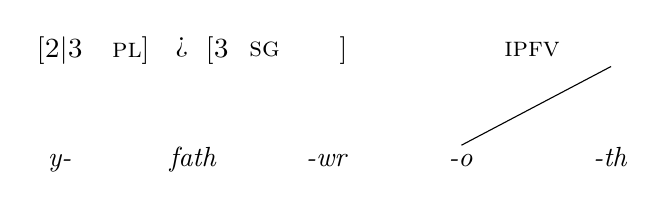
\begin{tikzpicture}
	\draw (7,1) --(5.1,0);
	\node[above] at (0,0.9) {[\Second\textbar\Third};
	\node[above] at (0.9,0.9) {\Pl]};
	\node[above] at (1.55,1) {>};
	\node[above] at (2,0.9) {[\Third};
	\node[above] at (2.6,1) {\Sg};
	\node[above] at (3.6,0.9) {\Masc]};
	\node[above] at (4.8,1) {\Nonpast};
	\node[above] at (6,1) {\Ipfv};
	\node[above] at (7.3,1) {\Andat};
	\node[below] at (0,0) {\emph{y-}};
	\node[below] at (1.7,0.1) {\emph{fath}};
	\node[below] at (3.4,0) {\emph{-wr}};
	\node[below] at (5.1,0) {\emph{-o}};
	\node[below] at (7,0.1) {\emph{-th}};
\end{tikzpicture}}
\end{center}
\caption{One-to-one mapping for the directional}
\label{one-to-one}
\end{figure}%one-to-one mapping with fathasi

Cumulative \isi{exponence} is found in the verb prefix \emph{y-} which fuses information on person (\Third), number (\Sg), and gender (\Masc) of the object argument. In addition, \emph{y-} contains information on tense (\Nonpast) and aspect (\Ipfv{}). This is schematised in Figure \ref{cumulfath}.

\begin{figure}
\begin{center}
\fbox{%
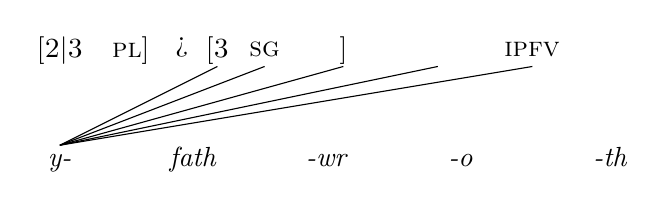
\begin{tikzpicture}
	\draw (2,1)   --(0,0);
	\draw (3.6,1) --(0,0);
	\draw (2.6,1) --(0,0);
	\draw (4.8,1) --(0,0);
	\draw (6,1) --(0,0);
	\node[above] at (0,0.9) {[\Second\textbar\Third};
	\node[above] at (0.9,0.9) {\Pl]};
	\node[above] at (1.55,1) {>};
	\node[above] at (2,0.9) {[\Third};
	\node[above] at (2.6,1) {\Sg};
	\node[above] at (3.6,0.9) {\Masc]};
	\node[above] at (4.8,1) {\Nonpast};
	\node[above] at (6,1) {\Ipfv};
	\node[above] at (7.3,1) {\Andat};
	\node[below] at (0,0) {\emph{y-}};
	\node[below] at (1.7,0.1) {\emph{fath}};
	\node[below] at (3.4,0) {\emph{-wr}};
	\node[below] at (5.1,0) {\emph{-o}};
	\node[below] at (7,0.1) {\emph{-th}};
\end{tikzpicture}}
\end{center}
\caption{Cumulative exponence of person, number, gender, tense and aspect}
\label{cumulfath}
\end{figure}%cumulative \isi{exponence} with fathasi

Note that the prefix \emph{y-} is necessary, but not sufficient, to establish the values for some of these categories. For example, the aspectual value of the \isi{verb} (\Ipfv) is not expressed solely by \emph{y-}. This is what Matthews calls ``extended \isi{exponence}'' (\citeyear[147-149]{Matthews:1979vm}) and Caballero \& Harris refer to as ``\isi{multiple exponence}'' (\citeyear[163]{Caballero:2012vr}). It is essentially the mirror image of Figure \ref{cumulfath}. Thus, Figure \ref{extendfath} below shows that \isi{aspect} is distributed over three exponents in \emph{yfathwroth}.

\begin{figure}
\begin{center}%
\fbox{
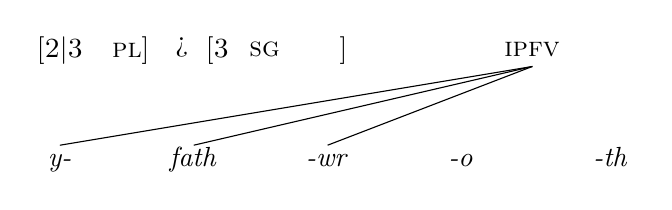
\begin{tikzpicture}
	\draw (6,1) --(0,0);
	\draw (6,1) --(1.7,0);
	\draw (6,1) --(3.4,0);
	\node[above] at (0,0.9) {[\Second\textbar\Third};
	\node[above] at (0.9,0.9) {\Pl]};
	\node[above] at (1.55,1) {>};
	\node[above] at (2,0.9) {[\Third};
	\node[above] at (2.6,1) {\Sg};
	\node[above] at (3.6,0.9) {\Masc]};
	\node[above] at (4.8,1) {\Nonpast};
	\node[above] at (6,1) {\Ipfv};
	\node[above] at (7.3,1) {\Andat};
	\node[below] at (0,0) {\emph{y-}};
	\node[below] at (1.7,0.1) {\emph{fath}};
	\node[below] at (3.4,0) {\emph{-wr}};
	\node[below] at (5.1,0) {\emph{-o}};
	\node[below] at (7,0.1) {\emph{-th}};
\end{tikzpicture}}
\end{center}
\caption{Extended exponence of aspect}
\label{extendfath}
\end{figure}%extended \isi{exponence} with fathasi

A change in any one of the three slots above will cause a change in the TAM value. For example, the prefix \emph{y-} can be replaced by \emph{su-} to form a \isi{recent past} \isi{imperfective} (\emph{sufathwroth}) or a suffix \emph{-m} can be added after \emph{-wr} to form a \isi{recent past} durative (\emph{yfathwrmoth}). If both of these changes are made at the same time, we get a \isi{past} durative (\emph{sufathwrmoth}). It follows that we are not dealing with a circumfix where separated formatives always occur together, but rather with a circumfixal paradigm where the formatives in the different slots are quite independent. Although there are some combinatorial restrictions, it would be a distortion to describe this as a circumfix. The essence of the system is that only by unifying the information from each slot are we in a position to calculate the correct value of a given grammatical category.%\\

Thus, the overall complexity of Komnzo verbs results from the co-ocurrence of different types of \isi{exponence} relationships. Figure \ref{recipfath} below captures all the dependencies between the values of a grammatical category and the morphs that make up \emph{yfathwroth}. Quite literally, we find a web of tightly interwoven dependencies.

\begin{figure}
\begin{center}
\fbox{%
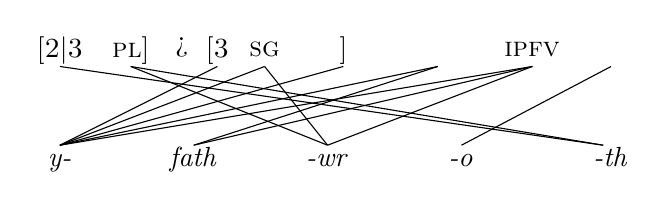
\begin{tikzpicture}
	\draw (0,1)   --(6.9,0);
	\draw (0.9,1) --(6.9,0);
	\draw (0.9,1) --(3.4,0);
	\draw (3.6,1) --(0,0);
	\draw (2.6,1) --(3.4,0);
	\draw (4.8,1) --(1.7,0);
	\draw (6,1) --(0,0);
	\draw (6,1) --(1.7,0);
	\draw (6,1) --(3.4,0);
	\draw (2,1)   --(0,0);
	\draw (2.6,1) --(0,0);
	\draw (4.8,1) --(0,0);
	\draw (7,1) --(5.1,0);
	\node[above] at (0,0.9) {[\Second\textbar\Third};
	\node[above] at (0.9,0.9) {\Pl]};
	\node[above] at (1.55,1) {>};
	\node[above] at (2,0.9) {[\Third};
	\node[above] at (2.6,1) {\Sg};
	\node[above] at (3.6,0.9) {\Masc]};
	\node[above] at (4.8,1) {\Nonpast};
	\node[above] at (6,1) {\Ipfv};
	\node[above] at (7.3,1) {\Andat};
	\node[below] at (0,0) {\emph{y-}};
	\node[below] at (1.7,0.1) {\emph{fath}};
	\node[below] at (3.4,0) {\emph{-wr}};
	\node[below] at (5.1,0) {\emph{-o}};
	\node[below] at (7,0.1) {\emph{-th}};
\end{tikzpicture}}
\end{center}
\caption{Reciprocal conditioning}\label{recipfath}
\end{figure}%\isi{reciprocal} conditioning with fathasi

Anderson uses the term ``\isi{reciprocal} conditioning'' (\citeyear[55]{Anderson:1992uw}) for this phenomenon, whereby exponents depend on several grammatical categories, while being underspecified for a single grammatical category.\footnote{Morpheme underspecifiation does not stop at the word boundary in Komnzo. For example, the actor argument in \emph{yfathwroth} can be either second or third person. Without context, this ambiguity can only be resolved by the personal pronouns. The same is true for future tense or event completion, which are expressed periphrastically with the preverbal particles \emph{kwa} and \emph{z} respectively.} I adopt the term ``\isi{distributed exponence}'' from Caballero \& Harris (\citeyear[170]{Caballero:2012vr}), who point out that it may be related to multiple/extended \isi{exponence}. Although it is excluded from the survey, Caballero \& Harris mention \isi{distributed exponence} in the theoretical discussion by explaining some aspects of Georgian \isi{verb} morphology (\citealt{Gurevich2006:geo}). Baerman (\citeyear{Baerman:2012ko}) describes a phenomenon that could also be called \isi{distributed exponence} for \ili{Nuer}, a Western Nilotic language. The complexity of marking case and \isi{number} in \ili{Nuer} builds on suffixes and stem alternations, which are independently manipulated and give rise to inflectional classes. Baerman stresses the noniconicity of the system ``in that these operations characterise simply a contrast of meaning, without being linked to any particular meaning'' (\citeyear[490]{Baerman:2012ko}). Similarly, Komnzo \isi{verb} morphology must be understood as a system where morphs contribute to a grammatical category, but a specific value of a given grammatical category requires information from several slots. Caroll provides the most detailed study of \isi{distributed exponence} in his grammar on \ili{Ngkolmpu} (\citeyear{Carroll:Ngkolmpu}), a related \ili{Tonda} language.%\\

There are practical consequences for the description of such a system. I have used a glossing style which follows the Word-and-Paradigm model (\citealt[67]{Matthews:1979vm}) throughout this grammar to give the reader effortless access to the morphosyntactic features of an inflected \isi{verb} form. Since this chapter addresses verbal morphology, I will employ a double glossing and a verb like \emph{yfathwroth} will be glossed as in (\ref{ex139}) below. The first line gives a maximally segmented \isi{gloss} in the Item-and-Arrangement style, while the second line in smaller print gives a unified \isi{gloss} in the Word-and-Paradigm style.\footnote{Elsewhere in the grammar - where there is no double glossing, but only the unified gloss - the verb stem is shown by slanted lines \stem{...} on the segmentation line.}

\begin{exe}
	\ex \emph{yfathwroth}\\
	\glll y-fath-w-r-o-th\\
	\Tsg.\Masc:\Alph-hold.\Ext-\Ndu-\Lk-\Andat-\Stnsg\\
	\footnotesize{\Stpl:\Sbj>\Tsg.\Masc:\Obj:\Nonpast:\Ipfv:\Andat/hold}\\
	\trans `They hold him away.'
	\label{ex139}
\end{exe}

The Item-and-Arrangement style provides more transparency in the morphological structure which is the aim of this chapter. In spite of that, widespread underspecification means that the gain in structural transparency comes at the cost of somewhat opaque glossing labels. For example, while we find in (\ref{ex139}) established labels like \Sg{} (\isi{singular}) and \Nsg{} (\isi{non-singular}) to encode \isi{number}, we also need to recruit \Ndu{} (\isi{non-dual}). As for \isi{tense} and \isi{aspect}, we have to introduce even more abstract labels like \Alph{} (alpha) in the prefixes or \Ext{} (extended) with the verb stem. These will be explained in the following sections. A further drawback of the Item-and-Arrangement style is that some of the grammatical values like non-past (\Nonpast) or imperfective (\Ipfv) as well as \isi{subject} (\Sbj), \isi{object} (\Obj) and \isi{indirect object} (\Io) cannot be shown on the \isi{gloss} line because they can be inferred only after integrating several exponents.

\section{Stem types} \label{roots-and-temp}

Komnzo verbal stems have two forms; an `\textsc{extended stem}' (\Ext) and a `\textsc{re-stricted stem}' (\Rs). As these labels indicate, the distinction is sensitive to \isi{aspect} without encoding a specific aspectual category. For now it is sufficient to state that the labels refer to the \isi{temporal} structure of the event, i.e. `extended in time' and `restricted in time'. The two stems differ (i) in their form, (ii) in the order of slots with respect to \isi{dual} marking and (iii) in their combinatorial possibilities with the \isi{prefix series}. I describe each point below.

\subsection{The formal relationship of extended and restricted stems} \label{formalrelationshipextrs}

Komnzo has pairs of \isi{verb} stems whose relationship is often unpredictable from any formal or semantic criteria. Nevertheless, there is a cline of similarity in form between the two stems which allows us to divide the verbal lexicon into seven classes (Table \ref{frbearr}). For thirty percent, there is a rule-based relation between the shapes of the two stems. At the other end of the spectrum, we find suppletive pairs of stems in five percent of the verbal lexicon. For more than two thirds of the lexicon the shape of the stems is unpredictable.%\\

\begin{table}
\caption{The formal relationship between \Ext{} and \Rs{} stem}
\begin{tabularx}{\textwidth}{llllrc}
\label{frbearr}\\
	\lsptoprule
	{class}&{rule} &\Ext{} &\Rs{} &{gloss} &{count}\\\midrule
	%\endfirsthead
% 	{class}&{rule} &\Ext{} &\Rs{} &{gloss} &{count}\\\midrule
	%\endhead
	\multirow{5}{*}{{i}}	&\multirow{5}{*}{\Ext{}=\Rs{}} &\multicolumn{2}{c}{\emph{mar-}} &see &\multirow{5}{*}{\textsc{42}}\\
	&&\multicolumn{2}{c}{\emph{zik-}} &turn off &\\
	&&\multicolumn{2}{c}{\emph{rikn-}} &destroy &\\
	&&\multicolumn{2}{c}{\emph{rmän-}} &close &\\
	&&\multicolumn{2}{c}{\emph{matukn-}} &shake &\\\midrule
	\multirow{5}{*}{{ii}} &\multirow{5}{*}{\Ext{}$\Leftarrow$\Rs-ak} &\emph{rfitfak}- &\emph{rfitf}- &answer &\multirow{5}{*}{\textsc{52}}\\
	&&\emph{morak}- &\emph{mor}- &lean &\\
	&&\emph{bthak}- &\emph{bth}- &finish &\\
	&&\emph{ritak}-	&\emph{rit}- &cross &\\
	&&\emph{msak}- &\emph{ms}-	&sit &\\\midrule
	\multirow{5}{*}{{iii}} &\multirow{5}{*}{\Ext-{c}$\Rightarrow$\Rs} &\emph{gar}- &\emph{garf}- &break &\multirow{5}{*}{\textsc{81}}\\
	&&\emph{fsi}- &\emph{fsir}- &count &\\
	&&\emph{tri}- &\emph{trinz}- &scratch &\\
	&&\emph{rni}- &\emph{rnith}- &smile &\\
	&&\emph{thari}- &\emph{tharif}-	&dig &\\\midrule
	\multirow{5}{*}{{iv}} &\multirow{5}{*}{{mutation}} &\emph{thwek}- &\emph{thweth}- &be glad &\multirow{5}{*}{\textsc{96}}\\
	&&\emph{mthek}- &\emph{mthef}- &lift up &\\
	&&\emph{moneg}-	&\emph{mones}- &wait &\\
	&&\emph{trakumg}- &\emph{trakumth}- &smash &\\
	&&\emph{bnaz}- &\emph{bnaf}- &wake up\\\midrule
	\multirow{5}{*}{{v}}	&\multirow{5}{*}{{irregular}} &\emph{rsör}- &\emph{rsöfäth}- & descend &\multirow{5}{*}{\textsc{26}}\\
	&&\emph{thorak}- &\emph{thothm}- &search &\\
	&&\emph{myukn}-	&\emph{myuf}- &twist &\\
	&&\emph{rirkn}-	&\emph{rirkfth}- &avoid	&\\
	&&\emph{tur}- &\emph{turam}- &kiss &\\\midrule
	\multirow{6}{*}{{vi}} &\multirow{6}{*}{{suppletive}} &\emph{re}- &\emph{zigrthm}- &look around &\multirow{6}{*}{\textsc{15}}\\
	&&\emph{ru}- &\emph{mg}-&shoot, spear &\\
	&&\emph{fn}- &\emph{kwr}-&hit, kill &\\
	&&\emph{na}- &\emph{znob}-&drink &\\
	&& \emph{zä}- & \emph{thor}-&carry &\\
	&&\emph{si}- &\emph{füs}- &cook &\\\midrule
	&\Rs{} {only} &- & \emph{-kuk}\textsuperscript{a} &stand &1 \\
	{vii}&\multirow{2}{*}{\Ext{} {only}} &\emph{rug}- &- &sleep&\multirow{2}{*}{6}\\
	&&\emph{rmug}- &- &envy &\\\midrule
	\textsc{total}&&&&&319\\
	\lspbottomrule
	\multicolumn{6}{l}{{\footnotesize \textsuperscript{a} This verb has a second stem \emph{-kogr}, which I analyse as a \isi{positional} stem (see \S\ref{positionalverbs}}).}\\
\end{tabularx}%The formal relationship between \Ext{} and \Rs{} stem
\end{table}


In class I, which makes up 13\% of verbs, the two stems are identical (\Ext{}=\Rs{}). Class II verbs (16\%) derive their extended stems from the \isi{restricted stem} with a suffix (\Ext{}=\Rs-\emph{ak}). Thus class I and class II make up that portion of the verb lexicon with a rule-based relationship between the two stems. However, only a few generalisations can be made about the scope of the rule, i.e. given a particular lexeme, one cannot decide straightforwardly which class it belongs to. Amongst those few generalisations is the fact that most verbs in class I end in /n/, but this is not true of all. Moreover, verbs ending in /n/ are also found in the other classes.%\\

The majority of verbs involve unpredictable changes at the right edge of the stem. In class III, which makes up 25\% of verbs, a consonant is added to the \isi{extended stem} in order to form the \isi{restricted stem} (\Rs=\Ext-\textsc{c}). The stem pairs of class IV verbs (30\%) involve final consonant mutation. In class III and IV, the affected consonants are not conditioned by the phonological environment. Class V verbs (8\%) are irregular, i.e. the difference involves more than the last consonant. The stems of class VI (5\%) are fully suppletive. Finally, a handful of verbs in class VII are defective, and have only one of the two stems.%\\

We can make a few observations from Table \ref{frbearr}. First, we find a cline of similarity which ranges from identity of the two stems to suppletive pairs with the bulk of verbs between the two extremes. Classes II\textendash{}V all have in common that the difference in form occurs the right edge of stem. Secondly, the classes and processes (consonant mutation, consonant addition, suffixation of \emph{-ak}) are neither phonologically conditioned, nor can we detect a semantic basis for them. Thirdly, the system shows little productivity, which I take as evidence for lexicalisation. In Table \ref{frbearr}, it is only class II for which a regular process can be formulated; the suffixation of \emph{-ak}. Finally, we find that for almost all verbs, both stems are attested. As a result, virtually all verbs can be inflected for the entire range of TAM categories, which leaves little role to play for lexical \isi{aspect} (or Aktionsart) in Komnzo.%\\

I will offer a historical explanation below (see \S{}\ref{comparativenoteextrs}) as to how the two stems have evolved in Komnzo and in the \ili{Tonda} subgroup more generally.

\subsection{Dual marking with extended and restricted stems} \label{dualextrs}

The most salient difference between the two stems is the location of the \isi{dual} marker, which follows the \isi{extended stem} but precedes the \isi{restricted stem}. I describe number marking in detail in \S{}\ref{numbersubsec}. In the examples (\ref{ex141}-\ref{ex143}) and (\ref{ex145}-\ref{ex147}), I contrast the imperfective and perfective imperatives of `hit'. The former often has a continuative interpretation (`keep on x-ing!') while the latter points to inception (`start doing x!'). In (\ref{ex140}) and (\ref{ex144}), all grammatical categories are held constant, and only the actor argument is cycled through the three number values. In (\ref{ex141}-\ref{ex143}), \isi{dual} is shown by a suffix (\emph{-n}), which contrasts with a \isi{non-dual} (\emph{-z}). In (\ref{ex145}-\ref{ex147}), \isi{dual} is expressed by a \isi{zero} which contrasts with a \isi{non-dual} prefix (\emph{a-}).

\begin{exe}
\ex
\label{ex140}
\begin{xlist}
	\ex %\textit{be fi sfnzé!}\\
	\glll \emph{be} \emph{fi} \emph{s-fn-z-é}\\
	 \Ssg{}.\Erg{} \Third{}.\Abs{} \Tsg{}.\Masc{}:\Bet{}-hit.\Ext{}-\Ndu{}-\Ssg{}.\Imp{}\\
	 {} {} \footnotesize{\Ssg:\Sbj>\Tsg.\Masc:\Obj:\Imp:\Ipfv/hit}\\
	\trans `You keep hitting him!'
	\label{ex141}
	\ex %\textit{bné fi sfnne!}\\
	\glll \emph{bné} \emph{fi} \emph{s-fn-n-e}\\
	 \Snsg{}.\Erg{} \Third{}.\Abs{} \Tsg{}.\Masc{}:\Bet{}-hit.\Ext{}-\Du{}-\Snsg{}.\Imp{}\\
	  {} {} \footnotesize{\Sdu:\Sbj>\Tsg.\Masc:\Obj:\Imp:\Ipfv/hit}\\
	\trans `You (2) keep hitting him!'
	\label{ex142}
	\ex %\textit{bné fi sfnze!}\\
	\glll \emph{bné} \emph{fi} \emph{s-fn-z-e}\\
	 \Snsg{}.\Erg{} \Third{}.\Abs{} \Tsg{}.\Masc{}:\Bet{}-hit.\Ext{}-\Ndu{}-\Snsg{}.\Imp{}\\
	  {} {} \footnotesize{\Spl:\Sbj>\Tsg.\Masc:\Obj:\Imp:\Ipfv/hit}\\
	\trans `You (3+) keep hitting him!'
	\label{ex143}
\end{xlist}
\end{exe}%ex140a-c
\begin{exe}
\ex
\label{ex144}
\begin{xlist}
	\ex %\textit{be fi sakwer!}\\
	\glll \emph{be} \emph{fi} \emph{s-a-kwr-\Zero{}}\\
	\Ssg{}.\Erg{} \Third{}.\Abs{} \Tsg{}.\Masc{}:\Bet{}-\Ndu{}-hit.\Rs{}-\Ssg{}.\Imp{}\\
	{} {} \footnotesize{\Ssg:\Sbj>\Tsg.\Masc:\Obj:\Imp:\Pfv/hit}\\
	\trans `You hit him!'
	\label{ex145}
	\ex %\textit{bné fi skwre!}\\
	\glll \emph{bné} \emph{fi} \emph{s-\Zero{}-kwr-e}\\
	\Snsg{}.\Erg{} \Third{}.\Abs{} \Tsg{}.\Masc{}:\Bet{}-\Du{}-hit.\Rs{}-\Snsg{}.\Imp{}\\
	{} {} \footnotesize{\Sdu:\Sbj>\Tsg.\Masc:\Obj:\Imp:\Pfv/hit}\\
	\trans `You (2) hit him!'
	\label{ex146}
	\ex %\textit{bné fi sakwre!}\\
	\glll \emph{bné} \emph{fi} \emph{s-a-kwr-e}\\
	\Snsg{}.\Erg{} \Third{}.\Abs{} \Tsg{}.\Masc{}:\Bet{}-\Ndu{}-hit.\Rs{}-\Snsg{}.\Imp{}\\
	{} {} \footnotesize{\Spl:\Sbj>\Tsg.\Masc:\Obj:\Imp:\Pfv/hit}\\
	\trans `You (3+) hit him!'
	\label{ex147}
\end{xlist}
\end{exe}%ex144a-c

The post-stem \isi{non-dual} marker, \emph{-z} in (\ref{ex140}), has a number of phonologically conditioned allomorphs (see \S{}\ref{allomorphdualsuffix}). The \isi{dual} marker is always \emph{-n}. In terms of segmentation, the post-stem slot is simple to recognise. This is not the case with the pre-stem duality marker which is \isi{zero} for \isi{dual} and \emph{a-} for \isi{non-dual} in (\ref{ex144}). For purposes of illustration, I have selected the imperatives here because the segmentation is clearest. In other parts of the paradigm, segmentation is messier because the \isi{dual} marker fuses with the \isi{valency change} prefix resulting in an ablaut contrast; \emph{a-} for \isi{dual} and \emph{ä-} for \isi{non-dual} (see \S{}\ref{prerootdual}). From a historical perspective, this structural split between a pre-stem and a post-stem slot is a way of preserving \isi{dual} marking after the original suffix had fused with the stem (see \S{}\ref{comparativenoteextrs}).

\subsection{The combinatorics of extended and restricted stems} \label{combinatoricsextrs}

Extended and restricted stems taken alone are underspecified for a particular TAM value and information from other morphological sites is required. With respect to the five \isi{prefix series} \Alph, \Bet{}, \Betaone{}, \Betatwo, \Gam{} (see \S{}\ref{personsuffsection}), the two stems differ in their combinatorial possibilities. For example, the \Alph{} prefixes combine with the \isi{extended stem} and the \Gam{} prefixes combine with the \isi{restricted stem}, but not vice versa. The \Alph{} series is recruited to form \isi{non-past}, \isi{immediate past}, \isi{recent past} or \isi{past} in \isi{imperfective} or \isi{durative} \isi{aspect} depending on suffixal material. The \Gam{} series is employed for \isi{recent past} or \isi{past}, both \isi{perfective}. The \Bet{} prefixes combine with both stems to form imperatives and irrealis with \isi{imperfective} and \isi{perfective} \isi{aspect}. The \Betaone{} and \Betatwo{} prefixes combine with the \isi{extended stem} (the latter exclusively so) to form \isi{recent past} and \isi{past} in \isi{imperfective} or \isi{durative} \isi{aspect}, again depending on suffixal material. The \Betaone{} prefixes combine with the \isi{restricted stem} to form an \isi{iterative}. The details of the five \isi{prefix series} as well as the aspectual distinctions will be addressed in \S{}\ref{combitam}. For present purposes, it is sufficient to stress that there are some limitations on the combinatorial possibilities for extended and restricted stems.

\subsection{A comparative note on multiple stems} \label{comparativenoteextrs}

Verb stem pairs which are sensitive to \isi{aspect} are known from other Papuan languages, for example \ili{Mian} (\citealt[245]{Fedden:2011wu}). In the Southern New Guinea region, \ili{Marind} shows striking architectural similarities to the Komnzo system. Drabbe reports on 4 verb classes in \ili{Marind} (\citeyear[31]{Drabbe:1955tm}). The first two classes which make up the main distinction are labelled ``momentaan'' versus ``duratief.'' Members of a third class can be both, and only the affixes signal the aspectual value of an inflected verb form. The fourth class is characterised as ``momentaan,'' but it can be turned into ``duratief'' by suffixing \emph{-a(t)}. The overall design of the \ili{Marind} system looks similar once we equate ``duratief'' with extended and ``momentaan'' with restricted. Drabbe's third class in \ili{Marind} bears resemblance to that group of Komnzo verbs where only one form is attested (class I in Table \ref{frbearr}). The fourth class is very close to those stem pairs in Komnzo which add the suffix \emph{-ak} to the \isi{restricted stem} in order to form the \isi{extended stem} (class II in Table \ref{frbearr}). Moreover, the two suffixes, \emph{-a(t)} in \ili{Marind} and \emph{-ak} in Komnzo, are formally similar. However, neglecting Drabbe's group three and four, the \ili{Marind} system differs in that most verbs fall into either ``momentaan'' or ``duratief.'' As we have seen above, almost all verbs in Komnzo have both stems.%\\

Within the Yam family, multiple verb stems are found in the \ili{Nambu} as well as the \ili{Tonda} subgroup. However, the system as laid out here seems to be more developed in the \ili{Tonda} languages. Pairs of verb stems are attested in \ili{Arammba}, where Boevé \& Boevé (\citeyear{Bouve:2003ar}) label them ``common root'' and ``limited action root.'' In my own fieldwork, I found stem pairs in \ili{Anta}, \ili{Wára}, \ili{Wèré}, Kámá, \ili{Kánchá}, \ili{Blafe}, Ránmo and \ili{Wartha} Thuntai. As for \ili{Ngkolmpu}\footnote{\ili{Ngkolmpu}, as well as Bädi, Smerky and Sota, were classified as varieties of \ili{Kanum} in the past.}, there are up to three stems for some verbs and these are sensitive to \isi{aspect} as well as verbal number (\citealt{Carroll:Ngkolmpu}). More descriptive work is needed to understand how the two stems are employed in the respective TAM systems of these languages.%\\

I will offer a first tentative historical explanation based on the comparison of duality/TAM marking and multiple stems within the Yam family. In the \ili{Nambu} subgroup, aspect-sensitive stems are only a marginal phenomenon. However, part of the verb inflection is a suffix which combines aspectual information with dual marking. For example, in \ili{Nen} (\citealt{Evans:2015to}) and \ili{Nama} (\citealt{Siegel:2015bp}) a thematic suffix follows the verb stem encoding TAM plus dual versus non-dual. In Komnzo, the suffix following the stem encodes only duality, but the presence versus absence of this suffix is determined by the stem type. Thus, it is involved in marking \isi{aspect} (see \S{}\ref{dualextrs}).%\\

I have shown above that the differences in form between the two stem types are located at the right edge. It is therefore a likely scenario that multiple stems have emerged through a process of demorphologisation (\citealt[154]{Hopper:1990vm}), i.e. through a fusion of suffixal material with the stem. Until more decriptive material is available, we are left to speculate on the nature of the original system. Logically, there are at least two possibilities: (i) the original suffix followed the \ili{Nambu} pattern encoding TAM and duality simultaneously or (ii) there were separate suffixes for each category. Since both the occurrence of multiple stems as well as cognate forms are attested in all varieties of the \ili{Tonda} languages, demorphologisation would constitute an innovation, which supports \ili{Tonda} as a subgroup of the Yam family. This is of some importance, because other systematic differences between \ili{Nambu} and \ili{Tonda}, like word-initial \isi{velar} \isi{nasals}\footnote{The \ili{Nambu} language Dre which is spoken close to other \ili{Tonda} languages has preserved initial velar nasals.} or gender marking on verbs, can be explained by assuming the loss of a particular feature in \ili{Nambu} rather than assuming an innovation in \ili{Tonda}.%\\

The historical scenario advanced above gave rise to different inflectional patterns within the \ili{Tonda} subgroup. Languages further to the west including \ili{Blafe}, Ránmo, \ili{Wartha} Thuntai and to some extent \ili{Kánchá} have lost \isi{dual} marking except in some high \isi{frequency} verbs like the copula. Other varieties like \ili{Wára}, \ili{Anta} and Komnzo have kept post-stem \isi{dual} marking for one stem type, but requisitioned a different slot in the template for the other stem type. This would explain why, in terms of morphological segmentation, the pre-stem \isi{dual} marking with restricted stems is much messier than post-stem \isi{dual} marking with extended stems (compare \S{}\ref{dualextrs} and \S{}\ref{prerootdual}). We could say that in a historical process, \isi{dual} marking has ``hijacked'' a slot which was hitherto solely employed for marking \isi{valency}. A third pattern is attested in \ili{Wèré}, where \isi{dual} marking is consistently post-stem for both stem types. However, irregularities involving a vowel change in the prefixes for some parts of the paradigm show that the \ili{Wèré} pattern is a case of regularisation of the Komnzo system rather than an independent development.%\\

The scenario developed here has to be treated with some caution, as there are exceptions to the generalisations made above. For example, \ili{Nen} has multiple stems for a few verbs like $\sqrt{}$\emph{waram} versus $\sqrt{}$\emph{warama} `give', encoding \isi{imperfective} and \isi{perfective} \isi{aspect} respectively (\citealt{Evans:nen}). Another exception is the \ili{Nambu} language \ili{Nä}, which has pre-stem \isi{dual} marking for some middle verbs. Much more comparative work needs to be done to fully account for the emergence of multiple verb stems in these languages.

\section{Alignment and verb templates} \label{alignmtemplates}

\subsection{Grammatical relations} \label{grammrel}

This section describes the argument structure in Komnzo. The term is understood as ``the configuration of arguments that are governed by a particular lexical item'' (\citealt[1130]{HaspelmathBardey:2004}). For the purpose of defining argument structure, we need to take into account particular constructions (\citealt[433]{Bickel:2011wo}). In Komnzo, these are \isi{case} and agreement (i.e. verb indexing). There are no other constructions restricted to a set of arguments (e.g. control, relativisation, \isi{coordination}, \isi{nominalisation} of verbs).%\\

First, I identify generalised semantic roles (\textsc{gsr}s) for each verb form. Following Bickel (\citeyear{Bickel:2011wo}), these roles are labelled as follows: A is the most agent-like argument and P is the most patient-like argument of a \isi{transitive} \isi{verb}, S is the sole argument of an \isi{intransitive} verb. For \isi{ditransitive} verbs, T is the most theme-like argument and R the most recipient-like argument.%\\

In the following, I will outline the two parameters of argument structure in Komnzo. In (\ref{ex752}-c), I show the basic structure for one-argument and two-argument predicates in a reduced glossing style. A is assigned \isi{ergative} \isi{case}, while S and P are assigned \isi{absolutive} \isi{case}. Example (\ref{ex754}) shows that A is indexed in the suffix and P is indexed in the prefix. S has to be split into S\textsubscript{P}, which is indexed in the prefix (\ref{ex752}), and S\textsubscript{A}, which is indexed in the suffix (\ref{ex753}). The underlying factor is the \isi{dynamicity} of the predicate (see \S\ref{prefixingverbsec}).

\begin{exe}
\ex
\label{ex751}
\begin{xlist}
	\ex %\textit{fi ykogr.}\\
	\gll \emph{fi} \emph{y-kogr}\\
	\Third(\Abs) \Tsg.\Masc-stand\\
	\trans `He stands.'
	\label{ex752}
	\ex %\textit{fi ŋamränzrth.}\\
	\gll \emph{fi} \emph{ŋamränzr-th}\\
	\Third(\Abs) stroll-\Tpl\\
	\trans `They stroll around.'
	\label{ex753}
	\ex %\textit{nafa fi yfnzrth.}\\
	\gll \emph{nafa} \emph{fi} \emph{y-fnzr-th}\\
	\Tpl{}.\Erg{} \Third(\Abs) \Tsg.\Masc-hit-\Tpl{}\\
	\trans `They hit him.'
	\label{ex754}
\end{xlist}
\end{exe}

Examples (\ref{ex756}-c) show the argument structure for three-argument predicates. Note that I discuss why there are some problems in describing ditransitives in \S\ref{ambifixingtemp}. For \isi{case} assignment, the examples show that P and T are marked by the \isi{absolutive} \isi{case} and R by the \isi{dative} \isi{case}. The R is always indexed in the prefix, not P nor T. Furthermore, the verb form is inflected with the \emph{a-} prefix, which I label \Vc{} for \isi{valency change}.

\begin{exe}
\ex
\label{ex755}
\begin{xlist}
	\ex %\textit{nafa fi yfnzrth.}\\
	\gll \emph{nafa} \emph{giri} \emph{nafan} \emph{y-a-rithr-th}\\
	\Tpl{}.\Erg{} knife(\Abs) \Tsg.\Dat{} \Tsg.\Masc-\Vc-give-\Tpl{}\\
	\trans `They give him the knife.'
	\label{ex756}
	\ex %\textit{nafa fi yfnzrth.}\\
	\gll \emph{nafa} \emph{bone} \emph{zokwasi} \emph{nzun} \emph{w-a-rbänzr-th}\\
	\Tpl{}.\Erg{} \Ssg.\Poss{} speech(\Abs) \Fsg.\Dat{} \Fsg-\Vc-explain-\Tpl{}\\
	\trans `They explain your message to me.'
	\label{ex757}
	\ex %\textit{nafa fi yfnzrth.}\\
	\gll \emph{nafa} \emph{srak} \emph{nafan} \emph{y-a-brigwr-th}\\
	\Tpl{}.\Erg{} boy(\Abs) \Tsg.\Dat{} \Tsg.\Masc-\Vc-return-\Tpl{}\\
	\trans `They return the boy for/to him.'
	\label{ex758}
\end{xlist}
\end{exe}

From the types of argument structure shown above, we can define the following \isi{grammatical relations} in Komnzo:

\begin{enumerate}
	\item The \isi{subject} relation is characterised by either \isi{ergative} or \isi{absolutive} case assignment.
	\begin{enumerate}
		\item If the noun phrase is in the \isi{ergative}, it will always be indexed in the suffix.
		\item If the noun phrase is in the \isi{absolutive}, it may be indexed in the suffix or the prefix. It is considered to be a \isi{subject}, iff the clause contains no ergative-marked noun phrase.
	\end{enumerate}
	\item The \isi{object} relation is characterised by \isi{absolutive} case assignment and indexation in the prefix. This only applies in the presence of another \isi{ergative} noun phrase which is indexed in the suffix.
	\item The \isi{indirect object} relation is characterised by \isi{dative} (or \isi{possessive}) case assignment and indexation in the prefix. Additionally, the verb form receives the \isi{valency change} prefix \emph{a-}.
\end{enumerate}%\isi{grammatical relations}

Similar to other grammatical categories, for example TAM and \isi{number}, \isi{grammatical relations} are constructed by unifying information from different sites. These are the \isi{person} marking affixes and the diathetic prefix, but also the \isi{case} assignment on the respective noun phrases. I describe the \isi{person} marking affixes on the verb as the actor suffix and the \isi{undergoer} prefix.\footnote{I use a semantic definition of the term undergoer as that argument which is affected by the event.} However, in the unified \isi{gloss}, which is employed throughout this grammar, I use \Sbj{} (\isi{subject}), \Obj{} (\isi{object}) and \Io{} (\isi{indirect object}). A reviewer suggested to use \A{} (actor) und \U{} (\isi{undergoer}) and avoid using categories like \isi{subject} and \isi{object}. I agree that there is no strong evidence for a \isi{subject} category in Komnzo. Nevertheless, I employ the terms \isi{subject}, \isi{object} and \isi{indirect object} as metalinguistic labels that I find useful in communicating with other linguists. I do not claim that these play an overly important role in the grammar of Komnzo. In addition, there are practical reasons for using \Sbj{} (\isi{subject}), \Obj{} (\isi{object}) and \Io{} (\isi{indirect object}) in the \isi{gloss} line. If I employ \A{} (actor) und \U{} (\isi{undergoer}), it would be impossible to show the distinction between an \isi{object} and an \isi{indirect object} in the unified \isi{gloss} line.

\subsection{Morphological templates}\label{morphologicaltemplates}

This section describes the structure of verbs by looking at the slots involved in the indexation of arguments. More precisely, I describe the arrangement of slots, the presence vs. absence of slots, as well as their content.%\\

Based on the inflectional pattern, Komnzo verbs can be classified into prefixing, \isi{middle} and ambifixing verbs, depending on whether prefix, suffix or both are employed. I use the term ``\isi{template}'' for the different inflectional patterns. Hence, we can say that a \isi{verb} form occurs in ``a prefixing \isi{template}'' or in ``an ambifixing \isi{template}''. These templates are lexically determined for some verb lexemes, which means we can speak of ``a prefixing verb'' or ``a \isi{middle} verb''. For the majority of verb lexemes, the system is flexible and verbs occur in different templates. We can describe a particular verb lexeme by stating that ``it occurs in the \isi{middle} template and the ambifixing template, but not in the prefixing \isi{template}''.%\\

The slots involved in the definition of templates are the following: (i) the \isi{undergoer} prefix, (ii) the diathetic prefix, and (iii) the actor suffix. The \isi{undergoer} prefix can index an argument, or it can be filled by the \isi{middle} prefix, which is person-invariant. The diathetic prefix can be absent or be filled by the \isi{valency change} prefix.\footnote{I use the neutral term ``valency change'' because its function is to either increase or decrease the valency of a verb.} The actor suffix can be either absent or present. Figure \ref{verbtemplatearg} provides a first schematic overview of the possible templates. Note that there are more than the three templates mentioned above. This is because the prefixing and the ambifixing template can be further subdivided depending on the presence versus absence of the \isi{valency change} prefix. Hence, there is a prefixing template and an \isi{indirect object} prefixing template; and there is a \isi{transitive} ambifixing template and a \isi{ditransitive} ambifixing template.

\begin{figure}

	\begin{tabularx}{\textwidth}{r|l|l|l|l|}
		\cline{2-2}\cline{4-4}
		{prefixing}:&\isi{undergoer} prefix &  & stem & \multicolumn{1}{l}{}\\ \cline{2-2}\cline{4-4}
		\multicolumn{4}{l}{}\\\cline{2-4}
		{\isi{indirect object} prefixing}:&\isi{undergoer} prefix & \Vc & stem & \multicolumn{1}{l}{}\\ \cline{2-4}
		\multicolumn{4}{l}{}\\\cline{2-5}
		{middle}:&\isi{middle} prefix & \Vc{} & stem & actor suffix\footnotemark\\ \cline{2-5}
		\multicolumn{4}{l}{}\\\cline{2-2}\cline{4-5}
		{\isi{transitive} ambifixing}:&\isi{undergoer} prefix & & stem & actor suffix\\ \cline{2-2}\cline{4-5}
		\multicolumn{4}{l}{}\\\cline{2-5}
		{\isi{ditransitive} ambifixing}:&\isi{undergoer} prefix & \Vc{} & stem & actor suffix\\ \cline{2-5}
		\multicolumn{4}{l}{}\\
	\end{tabularx}
\caption{Morphological templates and argument structure}
\label{verbtemplatearg}
\end{figure}%Morphological templates and argument structure
\footnotetext{The label `actor suffix' is problematic with some lexemes which employ the middle template for a passive function. In this case, the suffix encodes a patient argument (see \S{}\ref{middletemplatesubsection}).}

I briefly describe each template here and refer the reader to the subsequent sections in which a detailed description follows (\S{}\ref{prefixingverbsec}-6). In the prefixing template, only the \isi{undergoer} prefix is used for \isi{person} indexing. In the \isi{indirect object} prefixing template also, only the \isi{undergoer} prefix is used for \isi{person} indexing. However, the \isi{undergoer} prefix indexes an \isi{indirect object} (\isi{beneficiary} or \isi{possessor}). This is formally marked by the \isi{valency change} prefix \emph{a-}. In the \isi{middle} template, the prefix is filled by a \isi{middle} marker which is invariant for \isi{person} and \isi{number}. The sole argument is indexed in the suffix. The \isi{middle} marker is always followed by the \isi{valency change} prefix \emph{a-}. The \isi{middle} template is used for a variety of functions, and depending on the function of the argument in the suffix it may index an \isi{agent} or \isi{patient}. The ambifixing \isi{transitive} template uses both affixes for \isi{person} indexing. The prefix encodes the \isi{object} (\isi{patient}, \isi{theme}, \isi{experiencer}) and the suffix encodes the \isi{subject} (\isi{agent}, \isi{stimulus}). The \isi{ditransitive} ambifixing template follows the pattern of the \isi{transitive} template with the addition of the \isi{valency change} prefix \emph{a-}. The \isi{undergoer} prefix indexes the \isi{indirect object} (\isi{goal}, \isi{beneficiary}, \isi{possessor}).%\\

I illustrate the five templates with the verb \emph{migsi} `hang' in examples (\ref{ex760}-e). Note that although the system is flexible, i.e. verbs occur in different templates, there is only a small amount of \isi{verb} lexemes which can occur in all five templates. I choose the \isi{positional} verb \emph{migsi} `hang' in (\ref{ex759}). Positional verbs have a number of peculiarities, for example a special verbstem and \isi{stative} suffix, which also encodes \isi{number} (see \S\ref{positionalverbs}). This can be seen in (\ref{ex759}a) and  (\ref{ex759}b).

\begin{exe}
\ex
\label{ex759}
\begin{xlist}
	\ex \textsc{prefixing}:\\
	\gll \emph{y-mi-thgr}\\
	 	\Tsg.\Masc-hang.\Pos-\Stat.\Ndu\\
	\trans `He is hanging.'
	\label{ex760}

	\ex \textsc{\isi{indirect object} prefixing}:\\
	\gll \emph{y-a-mi-thgr}\\
	 	\Tsg.\Masc-\Vc-hang.\Pos-\Stat.\Ndu\\
	\trans `(Something) is hanging for him.'
	\label{ex761}

	\ex \textsc{middle}:\\
	\gll \emph{ŋ-a-mig-wr-\Zero}\\
	 	\M-\Vc-hang.\Ext-\Ndu-\Stsg\\
	\trans `It hangs itself up.'
	\label{ex762}

	\ex \textsc{\isi{transitive} ambifixing}:\\
	\gll \emph{y-mig-wr-\Zero}\\
	 	\Tsg.\Masc-hang.\Ext-\Ndu-\Stsg\\
	\trans `S/He hangs him up.'
	\label{ex763}

	\ex \textsc{\isi{ditransitive} ambifixing}:\\
	\gll \emph{y-a-mig-wr-\Zero}\\
	 	\Tsg.\Masc-\Vc-hang.\Ext-\Ndu-\Stsg\\
	\trans `S/He hangs it up for him.'
	\label{ex764}
\end{xlist}
\end{exe}

The templates do not align neatly with transitivity. For example, only a small minority of \isi{intransitive} verbs are prefixing (\ref{ex149}), while most employ a middle template (\ref{ex150}). The underlying semantic factor is the \isi{dynamicity} of the event (see \S{}\ref{prefixingverbsec}). On the other hand, the middle template covers a wide range of functions including reflexives and reciprocals, passives, as well as antipassives (see \S{}\ref{middletemplatesubsection}). Transitive verbs are usually expressed in the ambifixing template (\ref{ex151}). Ditransitive verbs occur in the ambifixing template with the addition of the \isi{valency change} prefix \emph{a-}, whereby an \isi{indirect object} is introduced to the clause. The corresponding noun phrase is flagged with \isi{dative} (\ref{ex152}) or \isi{possessive} \isi{case}, and it is indexed in the \isi{undergoer} prefix (see \S{}\ref{ambifixingtemp}).

\begin{exe}
\ex
\label{ex148}
\begin{xlist}
	\ex \textit{ktktme erfikwr.}\\
	\glll kt-kt=me e-rfik-wr\\
	 \Redup{}-group=\Ins{} \Stnsg{}:\Alph{}-grow.\Ext{}-\Ndu{}\\
	 {} \footnotesize{\Stpl:\Sbj:\Nonpast:\Ipfv/grow}\\
	\trans `They grow in groups.'
	\label{ex149}

	\ex \textit{nagayé ŋakwinth.}\\
	\glll nagayé ŋ-a-kwi-n-th\\
	 children \M{}:\Alph{}-\Vc{}-run.\Ext{}-\Du{}-\Stnsg{}\\
	  {} \footnotesize{\Stdu:\Sbj:\Nonpast:\Ipfv/run}\\
	\trans `The two children run.'
	\label{ex150}

	\ex \textit{nafa ŋad yrbänzrth.}\\
	\glll nafa ŋad y-rbä-nzr-th\\
	 \Tnsg{}.\Erg{} rope \Tsg.\Masc:\Alph{}-untie.\Ext{}-\Ndu{}-\Stnsg{}\\
	  {} {} \footnotesize{\Stpl:\Sbj>\Tsg.\Masc:\Obj:\Nonpast:\Ipfv/untie}\\
	\trans `They untie the rope.'
	\label{ex151}

	\ex \textit{nze nafan wawa yarithé.}\\
	\glll nze nafan wawa y-a-ri-th-é.\\
	 \Fsg{}.\Erg{} \Tsg.\Dat{} yam \Tsg{}.\Masc:\Alph{}-\Vc-give.\Ext{}-\Ndu{}-\Fsg{}\\
	  {} {} {} \footnotesize{\Fsg:\Sbj>\Tsg.\Masc:\Io:\Nonpast:\Ipfv/give}\\
	\trans `I give him the yam(s).'
	\label{ex152}
\end{xlist}
\end{exe}

{\renewcommand{\tabcolsep}{2pt}%
\begin{table}
\caption{Argument marking}
\label{argalignverbs}
	{\footnotesize%
	\begin{tabularx}{\textwidth}{p{1,6cm}p{2,5cm}p{1,4cm}p{2,1cm}lp{2,3cm}}
		\lsptoprule
		{template} &{semantic role} &{diathetic} &{semantic role} &{case} & {construction}\\
		&{in the prefix} &{prefix} &{in the suffix} &{frame} &\\\midrule
		% %\endfirsthead
		% {template} &{semantic role} &{diathetic} &{semantic role} &{case} & {construction}\\
		% &{in the prefix} &{prefix} &{in the suffix} &{frame} &\\\midrule
		% %\endhead
		prefixing&\isi{experiencer}, &\Zero{} &n/a &\Abs &intransitive\\
		&(agent)\textsuperscript{a} &&&&(stative)\\
		&&&&&\\
		indirect &beneficiary or &\emph{a-}	&n/a &\Dat{} or &intransitive\\
		\isi{object} &\isi{possessor} &&&\Poss &(stative)\\
		prefixing &&&&&\\
		&&&&&\\
		\isi{middle} &n/a &\emph{a-} &agent &\Abs	&intransitive\\
		&&&&&(dynamic)\\
		&&&&&\\
		\isi{middle} &n/a &\emph{a-} &agent &\Abs	&\isi{impersonal}\\
		&&&&&\\
		\isi{middle} &n/a &\emph{a-} &\isi{patient} &\Abs &\isi{passive}\\
		&&&&&\\
		\isi{middle} &n/a &\emph{a-} &agent &\Abs	&reflex. \& recip.\\
		&&&&&\\
		\isi{middle} &n/a &\emph{a-} &agent &\Erg{} (\Abs)\textsuperscript{b}	& suppressed-\\
		&&&&&\isi{object}\\
		&&&&&\\
		\isi{transitive} ambifixing &\isi{patient}, \isi{theme} &\Zero &agent	&\Erg{} \Abs{} &\isi{transitive}\\
		&&&&&\\
		\isi{transitive} ambifixing &\isi{experiencer} &\Zero &\isi{stimulus}	&\Abs{} \Erg{} &\isi{experiencer-object}\\
		&&&&&\\
		\isi{ditransitive} ambifixing &beneficiary, \isi{goal} &\emph{a-} &agent &\Erg{} \Abs{} \Dat &\isi{ditransitive}\\
		&&&&&\\
		\isi{ditransitive} ambifixing &\isi{possessor} &\emph{a-} &agent &\Erg{} \Abs{} \Poss &\isi{ditransitive}\\
		\lspbottomrule
		\multicolumn{6}{l}{\footnotesize{\textsuperscript{a} This is a marginal pattern as almost all prefixing verbs have stative semantics.}}\\
		\multicolumn{6}{l}{\footnotesize{\textsuperscript{b} In \isi{suppressed-object} clauses, the \isi{object} is suppressed from the indexation in the verb.}}\\
	\end{tabularx}}
\end{table}}%Argument marking

It follows that the \isi{valency change} prefix \emph{a-} (\Vc) has a double function. It increases and decreases the \isi{valency} of a \isi{verb}. This is exemplified with \emph{migsi} `hang' in examples (\ref{ex760}-e) above. There are a number of \isi{deponent} verbs attested, for example prefixing verbs or \isi{transitive} ambifixing verbs which obligatorily take the \emph{a-} prefix. I analyse them as \isi{deponent} in the sense of Baerman et al (\citeyear{Baerman:2006depo}) because in these cases the \isi{undergoer} prefix indexes a direct \isi{object}, although the presence of the \Vc{} prefix suggests an \isi{indirect object}.\footnote{Deponency is defined as a ``mismatch between morphology and morpho-syntax'' (\citealt{Baerman:2006depo}).}%\\

Table \ref{argalignverbs} provides a fine-grained overview of the templates. I show the semantic roles of the arguments indexed in the affixes, the presence/absence of the \isi{valency change} prefix, the \isi{case} frame and the name of the corresponding construction. These constructions are described in the section on clause types (\S\ref{clause types}).

\subsection{Valency alternations} \label{valencyalternations}

In Komnzo, \isi{valency alternations} are achieved by placing the \isi{verb} in different templates. There is only a handful of verbs which occur in all the templates. I choose the verb \emph{msaksi} `sit, dwell' to show its possibilities below with text examples (\ref{ex320}-\ref{ex323}). Note that \emph{msaksi} deviates in two ways from other verbs. First, it takes the \isi{valency change} prefix obligatorily when it occurs in a prefixing template, as can be seen in (\ref{ex320}). Secondly, there is a special verbstem for the prefixing template: \emph{m}. In other templates, \emph{msaksi} has the \isi{extended stem} \emph{msak} and the \isi{restricted stem} \emph{ms}, i.e. it is a class II verb (compare Table \ref{frbearr}).%\\

In example (\ref{ex320}), the speaker showed me a place which used to be inhabited by a spirit. He states that nobody knows where the spirit lives nowadays. Hence, the verb \emph{msaksi} has a \isi{stative} meaning in the prefixing template and can be translated into \ili{English} with `dwell, live, stay', or `be sitting'.

\begin{exe}
	\ex \emph{watik ŋafäniza ... ni miyamr mä zena \textbf{yamnzr}.}\\
	\glll watik ŋ-a-fäni-z-a-\Zero{} (.) ni miyamr mä zena y-a-m-nzr\\
	then \M.\Alph{}-\Vc-shift.place.\Ext-\Ndu-\Pst-\Stsg{} (.) \Fnsg{} ignorance where today \Tsg.\Masc.\Alph-\Vc-dwell.\Ext-\Ndu\\
	{} \footnotesize{\Stsg:\Sbj:\Ipfv:\Pst/shift.place} {} {} {} {} {} \footnotesize{\Tsg.\Masc:\Sbj:\Nonpast:\Ipfv/dwell}\\
	\trans `Then he shifted (location). We don't know where he lives today.'\\ \Corpus{tci20120922-19}{DAK \#37}
	\label{ex320}
\end{exe}

Example (\ref{ex321}) was uttered in the context of me visiting a garden place in the forest, where I was accompanied by the owner of the garden. The speaker happened to cycle past the garden place catching sight of me and the owner. The speaker comments on how he saw the two of us sitting down. Thus, \emph{msaksi} in the \isi{middle} template encodes a dynamic event and can be translated into \ili{English} with `sit down' or `assume a sitting position'.

\begin{exe}
	\ex \emph{nze nimäwä! boba thnmaré \textbf{ŋamsakrnmth}.}\\
	\glll nze nima=wä boba th-\Zero{}-n-mar-é\\
	\Fsg.\Erg{} like.this=\Emph{} \Med:\Abl{} \Stnsg.\Gam-\Du-\Venit-see.\Rs-\Fsg{}\\
	{} {} {} \footnotesize{\Fsg:\Sbj>\Stdu:\Obj:\Rpst:\Pfv:\Venit/see}\\
	\sn
	\glll ŋ-a-msak-rn-m-th\\
	\M.\Alph-\Vc-sit.\Ext-\Du-\Dur-\Stnsg{}\\
	\footnotesize{\Stdu:\Sbj:\Rpst:\Dur/sit}\\
	\trans `Me too! I saw you two from there and you were just sitting down.'\\ \Corpus{tci20130823-06}{STK \#90}
	\label{ex321}
\end{exe}

Example (\ref{ex322}) shows \emph{msaksi} in a \isi{transitive} ambifixing template. The example comes from a narrative, in which an angry man is forcefully seated and calmed down by giving him kava to drink.

\begin{exe}
	\ex \emph{wati \textbf{ymsakwrth} fof krär \textbf{yarinakwrth} bänemr fof nafane noku frazsir.}\\
	\glll wati y-msak-wr-th fof krär\\
	then \Tsg.\Masc.\Alph-sit.\Ext-\Ndu-\Stnsg{} \Emph{} kava\\
	{} \footnotesize{\Stpl:\Sbj>\Tsg.\Masc:\Obj:\Nonpast:\Ipfv/sit} {} {}\\
	\sn
	\glll y-a-rinak-wr-th bän=mr fof nafane noku\\
	\Tsg.\Masc.\Alph-\Vc-pour.\Ext-\Ndu-\Stnsg{} \Dem:\Med=\Purp{} \Emph{} \Tsg.\Poss{} anger\\
	\footnotesize{\Stpl:\Sbj>\Tsg.\Masc:\Io:\Nonpast:\Ipfv/pour} {} {} {}\\
	\sn
	\gll fraz-si=r\\
	extinguish-\Nmlz=\Purp{}\\
	\trans `So they sit him down properly and pour kava for him to cool down his anger.' \Corpus{tci20120909-06}{KAB 93-94}
	\label{ex322}
\end{exe}

Example (\ref{ex323}) is an elicited example showing \emph{msaksi} in a \isi{ditransitive} ambifixing template, where the \isi{undergoer} prefix indexes the \isi{possessor} (`his child'). Note that the same template is found in the second verb in (\ref{ex322}), where the \isi{undergoer} prefix indexes a \isi{beneficiary} (`pour kava for him').

\begin{exe}
	\ex \textit{nze nafange \textbf{yamsakwé}.}\\
	\glll nze nafa-nge y-a-msak-w-é.\\
	 \Fsg{}.\Erg{} \Third.\Poss-child \Tsg{}.\Masc{}:\Alph{}-\Vc{}-sit.\Ext{}-\Ndu{}-\Fsg{}\\
	  {} {} \footnotesize{\Fsg:\Sbj>\Tsg.\Masc:\Io:\Nonpast:\Ipfv/sit}\\
	\trans `I sit his child down.'
	\label{ex323}
\end{exe}

The above examples show that \isi{valency alternations} are achieved by using the same verb in different templates. It is important to note that all the inflected verb forms share the same \isi{infinitive}, which is formed by suffixing the \isi{nominaliser} \emph{-si} to the stem. In (\ref{ex324}) and (\ref{ex325}) I show the \isi{infinitive} with a \isi{stative} and a dynamic interpretation. Example (\ref{ex324}) is the conclusion of a short narrative about taboos and customs that involve the bird of paradise. The speaker uses \emph{msaksi} with a \isi{locative} \isi{case} suffix in a \isi{possessive} construction to express `in our life'. In example (\ref{ex325}), the speaker showed me a beautiful place on the bank of Morehead river. She comments that this is a good place to sit down and rest. Hence, the \isi{infinitive} \emph{msaksi} is used for both interpretations, a timeless state in (\ref{ex324}) and a dynamic event in (\ref{ex325}).

\begin{exe}
	\ex \emph{nzenme trtha mrmren nzenme \textbf{msaksin} ... wtrikarä anema fof ŋamränzre.}\\
	\gll nzenme trtha mrmr=en nzenme msak-si=n (.) wtri=karä\\
	\Fnsg.\Poss{} life inside=\Loc{} \Fnsg.\Poss{} sit-\Nmlz=\Loc{} (.) fear=\Prop{}\\
	\sn
	\glll ane=ma fof ŋ-a-mrä-nzr-e\\
	\Dem=\Char{} \Emph{} \M.\Alph-\Vc-stroll.\Ext-\Ndu-\Fnsg{}\\
	{} {} \footnotesize{\Fpl:\Sbj:\Nonpast:\Ipfv/stroll}\\
	\trans `In our way of life ... in our living ... we walk about with fear because of this.' \Corpus{tci20120817-02}{ABB \#40-43}
	\label{ex324}
\end{exe}
\begin{exe}
	\ex \emph{camp rä ... zmbo fthé nanyak \textbf{msaksir}.}\\
	\glll camp rä (.) zmbo fthé n-a-n-yak\\
	camp \Tsg.\F.\Cop.\Ndu{} (.) \Prox.\All{} when \Fnsg.\Alph-\Vc-\Venit-walk.\Ext.\Ndu{}\\
	{} \footnotesize{\Tsg.\F:\Sbj:\Nonpast:\Ipfv/be} {} {} {} \footnotesize{\Fpl:\Sbj:\Nonpast:\Ipfv/come}\\
	\sn
	\gll msak-si=r\\
	sit-\Nmlz=\Purp{}\\
	\trans `This is a camp ... We come here to sit down (and rest).'\\ \Corpus{tci20130907-02}{RNA \#331-333}
	\label{ex325}
\end{exe}

The meaning of a \isi{verb} in one template may differ substantially when used in another template. For example, the verb \emph{rfiksi} `grow' occurs in the prefixing template (\ref{ex149}), but it can be used in a \isi{transitive} ambifixing template with the meaning `nurture' (Lit. `grow somebody'). A second example is the verb \emph{rbänzsi} `untie' which usually occurs in a \isi{transitive} ambifixing template (\ref{ex151}). Used in a \isi{ditransitive} ambifixing template it has the meaning `explain' (Lit. `untie for somebody'). Nevertheless, inflected verbs in different templates all share the same \isi{infinitive}. In this aspect Komnzo differs from other \ili{Yam languages}. For example in \ili{Nen}, there are no infinitives for prefixing verbs, but instead valency-altered forms have distinct infinitives which include the relevant formatives from a set of diathetic prefixes (\citealt{Evans:2015wy}). For example, one pair of infinitives is: \emph{amzs} `sit (v.i.)' versus \emph{wamzs} `set, sit (v.t.)'. There are even triplets: \emph{an\={g}ws} `return (v.i.)' versus \emph{wan\={g}ws} `return (v.t.)' versus \emph{wawan\={g}ws} `return to/for (v.t.)'. In Komnzo, there are no distinct infinitives for valency-altered forms. Hence, \emph{rfiksi} is the \isi{infinitive} of both `grow' and `nuture', and \emph{rbänzsi} is the \isi{infinitive} of `untie' and `explain'.%\\

There are two ways of analyzing shared infinitives in Komnzo and I argue that both are needed. On the one hand, we can understand it as a system where \isi{valency} is fluid and lexemes are flexible. Under this analysis a lexeme can alter its \isi{valency} by occuring in different templates. On the other hand, we could adopt the notion of \isi{heterosemy} (\citealt{Lichtenberk:1991ic} and \citealt[524]{Evans:2012we}) to capture that different lexical items and meanings are expressed by different templates.\footnote{This assumes a definition of the linguistic sign as having three parts: form, meaning and combinatorics (or syntax) as put forward by (\citealt{Melcuk:1973vu}) and (\citealt[51]{Pollard:1987wu}).} A verb like \emph{msaksi} shows that we need both perspectives. On the one hand, \emph{msaksi}\textsubscript{1} means `dwell, live' in a prefixing template, while \emph{msaksi}\textsubscript{2} means `sit down' in a middle/ambifixing template. We would understand \emph{msaksi}\textsubscript{1} as being heterosemous to \emph{msaksi}\textsubscript{2} because there is a significant shift in meaning due to the template. The same holds for pairs like \emph{rfiksi} meaning `grow' or `nuture' and \emph{rbänzsi} meaning `untie' or `explain'. On the other hand, the system of \isi{valency alternations} in Komnze is very productive. Especially the \isi{middle} template and the \isi{ditransitive} ambifixing template can be used for almost every verb which can also occur in the \isi{transitive} ambifixing template. Thus, describing the alternation between \emph{msaksi} in (\ref{ex322}) `sit someone down' and (\ref{ex323}) `sit down someone's (child)' in terms of \isi{heterosemy} would fall short of an exhaustive description. It would not adequately capture the productivity of the system, nor would it fully explain shared \isi{infinitive}s for verb forms of different templates.

\subsection{The prefixing template} \label{prefixingverbsec}

\subsubsection{Introduction}

Prefixing verbs are a small class with around 20 lexical items attested so far. Some of them can occur in other templates, but most occur only in the prefixing template. Table \ref{pref.verbs} lists all the members of the prefixing class. Furthermore, there is a class of 41 \isi{positional} verbs, which can occur in the prefixing template (see \S{}\ref{positionalverbs}).

{\renewcommand{\tabcolsep}{4pt}
\begin{table}
\caption{Prefixing verbs}
\label{pref.verbs}
	\begin{tabularx}{\textwidth}{Xlll}
		\lsptoprule
		{infinitive} &{gloss} &{possible} &{gloss}\\
		or {stem}\footnotemark &&{templates}&\\\midrule
		\emph{-rug}	&`sleep' &pref. only & -\\
		\emph{-yak}	&`walk, go'	&pref. only & -\\
		\textsuperscript{a}\emph{-nyak} &`come' &pref. only & -\\
		\textsuperscript{a}\emph{yathizsi} &`suffer' &pref. only & -\\
		\textsuperscript{a}\emph{mthizsi} &`rest' &pref. only & -\\
		\textsuperscript{a}\emph{-nor} &`shout, emit sound' &pref. only & -\\
		\emph{wäksi} &`be caught by daybreak' &pref. only & -\\
		\emph{fogsi} &`be caught by nightfall' &pref. only & -\\
		\emph{rmigfaksi} &`be in the middle of (doing) sth.'& pref. only &-\\
		\emph{-thn}	&`be lying'	&pref. only & -\\
		\textsuperscript{a}\emph{yarenzsi} &`look around' &pref. only & -\\
		\emph{-ythk} &`be finished' &pref. only & -\\
		\textsuperscript{a}\emph{namgsi}	&`be panting, gasping' &pref. only & -\\
		\emph{thfäsi} &`jump' &pref./middle	&`fly'\\
		\textsuperscript{a}\emph{thgusi}	&`forget' & pref./trans.  &`confuse sth.'\\
		\emph{thoraksi}	&`appear, arrive' & pref./trans.  &`find, search'\\
		\emph{wokraksi}	&`float' &pref./trans. &`make sth. float'\\
		\emph{-rä} &`be' &all templates &`do'\\
		\textsuperscript{a}\emph{msaksi}	&`dwell, live' &all templates &`sit (self or sb.)'\\
		\emph{sufaksi} &`grow old' &all templates &`bring to an end'\\
		\emph{ziksi} &`turn off, be on the side' &all templates &`put to the side'\\
		\emph{rfiksi} &`grow' &all templates &`nurture'\\
		\lspbottomrule
		\multicolumn{4}{l}{\footnotesize{\textsuperscript{a} These verbs are \isi{deponent}, i.e. they use the \Vc{} prefix obligatorily.}}\\
	\end{tabularx}
\end{table}}%Prefixing verbs
\footnotetext{Infinitives are marked with the nominaliser suffix \emph{-si}. Prefixing verbs are irregular in many respects. Some of the verbs listed here lack an infinitive and only the extended stem is given, while others employ a common noun as their infinitive, for example \emph{etfth} `sleep,' \emph{moth} `path, walk, come' and \emph{kwan} `noise, shout.' This does not correlate with whether there are other templates available. Where a nominalised form with \emph{-si} is lacking, I give the extended stem. Another irregularity are verbs where the stem is sensitive to the dual versus non-dual distinction, for example `walk' \emph{-yak} (\Ndu) versus \emph{-yan} (\Du) or `shout' \emph{-nor} (\Ndu) versus \emph{-rn} (\Du). In these cases, the non-dual stem is listed.}

Prefixing verbs are special in their morphology in that they can encode a fourth \isi{number} value. The somewhat odd combination of a \isi{non-singular} prefix and a \isi{dual} suffix yields a \isi{large plural}. This is attested in other \ili{Yam languages}, for example for \isi{positional} verbs in \ili{Nen} and \ili{Nä} (\citealt{Evans:2014bz}). I describe the four-way \isi{number} contrast in \S{}\ref{positonalnumber}.%\\

Prefixing verbs are mostly \isi{stative} in their semantics. Comparative work on split intransitivity has shown that differences in \isi{alignment} are often semantically motivated ( \citealt{Merlan:1985tu}, \citealt{Mithun:1991wu} and \citealt{Arkadiev:2008vq}). In Komnzo, the semantic parameters involved are the \isi{dynamicity} of the event and the \isi{volitionality} of the \isi{participant}, the former plays the dominant role. As we have seen in \S\ref{valencyalternations}, predicates in a prefixing template tend to be more \isi{stative} (\ref{ex320}), while predicates in \isi{middle} or ambifixing templates tend to be more dynamic (\ref{ex321}-\ref{ex323}). In other languages of the Yam family, the split between \isi{stative} and dynamic event types is congruent with the distinction between prefixing and \isi{middle} intransitives, for example in \ili{Nen} (\citealt{Evans:2015to}) and \ili{Nama} (\citealt{Siegel:2015bp}).\footnote{Siegel uses different terminology in his description of \ili{Nama}. What I call the prefixing template or stative intransitives equals ``patientive intransitives'', and what I label the middle template or dynamic intransitives equals ``agentive intransitives'' (\citealt[213]{Siegel:2015bp}).}%\\

In Komnzo, although all verbs in a middle or ambifixing template depict dynamic event types, we find a somewhat mixed picture with prefixing verbs. Table \ref{pref.verbs} contains a few dynamic events, for example \emph{-nor} `shout', \emph{thoraksi} `appear, arrive' and \emph{rfiksi} `grow'. In some cases, \isi{volitionality} is the semantic parameter involved in the prefixing/middle/ambifixing alternation: \emph{thoraksi} and \emph{rfiksi} in an ambifixing \isi{transitive} template mean `find' and `nurture' respectively.\footnote{In ambifixing templates, the case marking of a more agent-like argument is ergative. This is also found in middle templates with an suppressed-object function.} The verb \emph{-nor} `shout' allows no alternation, but occurs only in a prefixing template. Interestingly, \emph{-nor} is often used in a \isi{pseudo-cognate object} construction: \emph{kwan yannor}\footnote{\emph{-nor} lacks a nominalised infinitive and instead the common noun \emph{kwan} `shout, call' is used.} `He shouts (the shout)' or \emph{ya yannor} `He cries (the tears)'. Hence, with this verb a less volitional meaning like `emit a sound' might be licenced. Pseudo-\isi{cognate object} constructions are described in \S{}\ref{pseudocognate}. Nevertheless, with other predicates in Table \ref{pref.verbs} such an explanation fails, for example \emph{ziksi} `turn off, go in' or \emph{thfäsi} `jump'. Keeping the unusually small size of the prefixing class in mind, I interpret these cases as exceptions to the overall rule. Furthermore, the existence of a class of \isi{positional} verbs (\S{}\ref{positionalverbs}) underscores the split along the lines of event \isi{dynamicity} and \isi{volitionality}.%\\

All prefixing verbs can take the \isi{valency change} prefix \emph{a-}. This template was labelled \isi{indirect object} prefixing in Table \ref{argalignverbs}. However, in doing so they remain monovalent in their cross-referencing. The `additional argument', usually a Beneficiary or Possessor, replaces the `original argument', usually an Experiencer. However, the event itself remains to `be about' the original argument. A common usage of this pattern involves the \isi{copula}: When handing something to a person, one would say \emph{bnarä!} `There you are!' (literally: `(It) is there for you!'). A textual example comes from a stimulus task in which two speakers are describing the content of picture cards (\ref{ex160}). The picture in the example shows a policeman who hands some personal belongings to another man. After describing the scene, one of the two speakers points to a few things on the side asking what these were. The first verb in (\ref{ex160}) `be lying down' indexes the (assumed) \isi{possessor} and not the things on the ground. The second clause is accompanied by a pointing gesture in order to draw the interlocutor's attention to the objects. Here, the copula indexes the things on the ground.

\begin{exe}
	\ex \emph{mrmr ra \textbf{yathn}? zane \textbf{zerä}!}\\
	\glll mrmr ra y-a-thn zane\\
	inside what.\Abs{} \Tsg.\Masc.\Alph-\Vc-lie.\Ext.\Ndu{} \Dem:\Prox{}\\
	{} {} {\footnotesize \Tsg.\Masc:\Io:\Nonpast:\Ipfv/lie} {}\\
	\sn
	\glll z=e-rä\\
	\Prox=\Stnsg.\Alph-be.\Ext.\Ndu\\
	{\footnotesize \Prox=\Stpl:\Sbj:\Nonpast:\Ipfv/be}\\
	\trans `What are these (of his) inside? These ones here!' \Corpus{tci20111004}{TSA \#29-30}
	\label{ex160}
\end{exe}

Table \ref{pref.verbs} indicates that eight out of 20 prefixing verbs obligatorily use the \emph{a-} prefix without introducing an argument. I analyse these verbs as \isi{deponent} (\citealt{Baerman:2006depo}).

\subsubsection{Positional verbs} \label{positionalverbs}

The class of 41 \isi{positional} or postural verbs underscores the role of \isi{dynamicity} in the \isi{alignment} of S. Positional verbs express states of the type `be in position X' (`be leaning,' `be standing,' `be submerged' etc). Example (\ref{ex328}) shows the verb \emph{migsi} `hang'.%\\

\begin{exe}
	\ex \emph{bidrthatha zbo \textbf{sumithgrm} wämnen.}\\
	\glll bidr=thatha zbo su-mi-thgr-m wämne=n\\
	{{flying.fox}=\Simil{}} {\Prox.\All{}} \Tsg.\Masc.\Betaone{}-be.hanging-\Stat.\Ndu-\Dur{} tree=\Loc\\
	{} {} \footnotesize{\Tsg.\Masc:\Sbj:\Pst:\Dur:\Stat/be.hanging} {}\\
	\trans `He was hanging like a flying fox on the tree.' \Corpus{tci20130901-04}{RNA \#48}
	\label{ex328}
\end{exe}

Like most \isi{positional} verbs, \emph{migsi} can enter into other templates, for example a \isi{middle} template (`assume a hanging position') or a \isi{transitive} template (`hang something'). This is shown below in examples (\ref{ex326}) and (\ref{ex327}) respectively. Example (\ref{ex326}) is part of a plant walk around Rouku village. The speaker shows me a plant in the part of the land which is inundated during the rainy season. Example (\ref{ex327}) comes from a procedural text in which the speaker shows me around his yam storage house. He remarks that small yam suckers are called \emph{sagusagu} and they are stored by tying several yams into bundles.%\\

\begin{exe}
	\ex \emph{bubukr zä zf kwa \textbf{ŋamigwrth} ... watik kofäyé zbo zf kwa erkunzrth.}\\
	\glll bubukr zä zf kwa ŋ-a-mig-wr-th (.) watik kofä=é zbo zf kwa e-rku-nzr-th\\
	insect \Prox{} \Imm{} \Fut{} \M.\Alph-\Vc-hang.\Ext-\Ndu-\Stnsg{} (.) then fish=\Erg.\Nsg{} \Prox.\All{} \Imm{} \Fut{} \Stnsg.\Alph-knock.down.\Ext-\Ndu-\Stnsg\\
	{} {} {} {} \footnotesize{\Stpl:\Sbj:\Nonpast:\Ipfv/hang} {} {} {} {} {} {} \footnotesize{\Stpl:\Sbj>\Stpl:\Obj:\Nonpast:\Ipfv/knock.down}\\
	\trans `The insects will hang (themselves) from here and the fish will knock them down right here.' \Corpus{tci20130907-02}{RNA \#657}
	\label{ex326}
\end{exe}
\begin{exe}
	\ex \emph{nima yamme ane fof ŋafrmnzre bnrä ... \textbf{bemigwre} ane sagusagu.}\\
	\glll nima yam-me ane fof ŋ-a-frm-nzr-e \\
	like.this custom-\Ins{} \Dem{} \Emph{} \M.\Alph-\Vc-prepare.\Ext-\Ndu-\Fnsg{}\\
	{} {} {} {} \footnotesize{\Fpl:\Sbj:\Nonpast:\Ipfv/prepare}\\
	\sn
	\glll b=n-rä (.) b=e-mig-wr-e ane sagusagu\\
	\Med=\Fnsg.\Alph-\Cop.\Ndu{} (.) \Med=\Stnsg.\Alph-hang.\Ext-\Ndu-\Fnsg{} \Dem{} sagusagu\\
	\footnotesize{\Med=\Fpl:\Sbj:\Nonpast:\Ipfv/be} {} \footnotesize{\Med=\Fpl:\Sbj>\Stpl:\Obj:\Nonpast:\Ipfv/hang} {} {}\\
	\trans `We prepare them in this way ... We hang up those \emph{sagusagu}.'\\ \Corpus{tci20121001}{ABB \#38}
	\label{ex327}
\end{exe}

Positionals are attested in languages throughout the Yam family (\citealt{Evans:2014bz}). For Komnzo, I define them as a class of lexemes with \isi{positional} or postural semantics which share the following morphosyntactic properties: (i) the ability to occur in the prefixing template, (ii) the ability to take the \isi{stative} suffix \emph{-thgr}, (iii) the ability to form related \isi{middle} and \isi{transitive} \isi{verb} forms, and (iv) to inflect only for a subset of TAM categories when used in a prefixing template. Table \ref{positional.verbs} lists the 41 members of the class which are currently attested. We find both very general meanings (\emph{rzarsi} `be tied', \emph{yufaksi} `be bent over') and very specific meanings (\emph{rngthksi} `be stuck in a tree fork', \emph{mgthksi} `be in the mouth'). Some of these verbs occur with prototypical participants, for example \emph{zaksi} `be anchored' with \emph{garda} `canoe' or \emph{thamsaksi} `be spread out' with \emph{yame} `mat'.%\\

Table \ref{positional.verbs} compares the extended (\Ext) and \isi{restricted stem} (\Rs) and shows that for some verbs a \isi{positional} stem (\Pos) can be postulated. The \isi{positional} stem is the lexical base to which the \isi{stative} suffix \emph{-thgr} attaches. In the first two groups of Table \ref{positional.verbs}, the base is formally identical to the extended or \isi{restricted stem}. Only in the third group, is the base different from both, in that it is always shorter. The last group contains three lexemes which are irregular in a number of ways: (i) they take a slightly different form of the \isi{stative} suffix, which is given in parentheses for each, (ii) the last two lexemes in this group occur only as positionals, (iii) the second lexeme in the group lacks an infinitive.%\\

The data from Table \ref{positional.verbs} shows that for some of the verbs we need to posit a third stem type, the \isi{positional} stem, in addition to the extended and restricted stems we already encountered. The formal difference or similarity between the \isi{positional} stem and the other two stem types for a given lexeme cannot be predicted on semantic or phonological grounds, but must be seen as lexicalisation in a specific morphosyntactic context. Furthermore, one should keep in mind that \isi{positional} stems are not in a paradigmatic relationship of the kind we have seen with extended and restricted stems (\S{}\ref{roots-and-temp}). For example, the \isi{stative} semantics of positionals blocks all \isi{perfective} TAM categories.


\begin{table}
\caption{Positional verbs}
\label{positional.verbs}
{\small%
\begin{tabularx}{\textwidth}{Xllll}
	\lsptoprule
	{infinitive} & \Pos{} {stem} & \Ext{} \textsc{stem} 	& \Rs{} \textsc{stem} 	& {gloss} \\\midrule
	\emph{mosisi} &\emph{mosi-} &\emph{mosi-} &\emph{mosir-} &be gathered, piled\\
	\emph{moyusi} &\emph{moyu-} &\emph{moyu-} &\emph{moyuth-} &be shrunk\\
	\emph{rfakusi} &\emph{rfaku-} &\emph{rfaku-} &\emph{rfakuth-} &be sprinkled\\
	\emph{ttüsi} &\emph{ttü-} &\emph{ttü-} &\emph{ttüth-} &be printed, carved\\
	\emph{tharasi} &\emph{thar-} &\emph{thar-} &\emph{tharf-} &be underneath\\
	\emph{worsi} &\emph{wor-} &\emph{wor-} &\emph{won-} &be planted\\\midrule
	\emph{brüzsi} &\emph{brüs-} &\emph{brüz-} &\emph{brüs-} &be submerged\\
	\emph{krsi} &\emph{kr-} &\emph{krth-} &\emph{kr-} &be blocked off\\
	\emph{räzsi} &\emph{räs-} &\emph{räz-} &\emph{räs-} &be erected\\
	\textsuperscript{a}\emph{rfuthraksi} &\emph{rfuth-} &\emph{rfuthrak-} &\emph{rfuthr-} &be piled up\\
	\emph{rmithraksi} &\emph{rmithr-} &\emph{rmithrak-}	&\emph{rmithr-} &be joined together\\
	\emph{rmnzüfaksi} &\emph{rmnzüf-} &\emph{rmnzüfak-}	&\emph{rmnzüf-} &be side by side / parallel\\
	\emph{rthbraksi} &\emph{rthbr-} &\emph{rthbrak-} &\emph{rthbr-} &be sticking (on sth.)\\
	\emph{rzarsi} &\emph{rzaf-} &\emph{rzar-} &\emph{rzaf-} &be tied\\
	\emph{thamsaksi} &\emph{thams-} &\emph{thamsak-} &\emph{thams-} &be spread out\\
	\textsuperscript{a}\emph{yufaksi} &\emph{yuf-} &\emph{yufak-} &\emph{yuf-} &be bent\\
	\emph{zaksi} &\emph{z-} &\emph{zak-} &\emph{z-} &be anchored\\\midrule
	\emph{fätfaksi} &\emph{fät-} &\emph{fätfak-} &\emph{fätf-} &be across sth.\\
	\emph{fethaksi} &\emph{fe-} &\emph{fethak-} &\emph{feth-} &be dipped in water\\
	\emph{fifthaksi} &\emph{fif-} &\emph{fifthak-} &\emph{fifth-} &be lying straight\\
	\emph{migsi} &\emph{mi-} &\emph{mig-} &\emph{mir-} &be hanging\\
	\emph{moraksi} &\emph{mo-} &\emph{morak-} &\emph{mor-} &be leaning\\
	\textsuperscript{a}\emph{mgthksi} &\emph{mg-} &\emph{mgthk-} &\emph{mgthm-} &be in the mouth\\
	\emph{mreznsi} &\emph{mre-} &\emph{mrezn-} &\emph{mrezn-} &be straight\\
	\textsuperscript{a}\emph{mtheksi} &\emph{mthe-} &\emph{mthek-} &\emph{mthef-} &be lifted up \\
	\emph{myuknsi} &\emph{myu-}& \emph{myukn-} &\emph{myuf-} &be twisted\\
	\emph{nänzüthzsi} &\emph{nänzü-}& \emph{nänzüthz-} &\emph{nänzütham-} &be covered with soil\\
	\emph{rafigsi} &\emph{rafi-}&\emph{rafig-} &\emph{rafinz-} &be on top of sth.\\
	\emph{rakthksi}	&\emph{rak-}&\emph{rakthk-} &\emph{rakthm-} &be on top of sth.\\
	\emph{rinaksi} &\emph{ri-}& \emph{rinak-} &\emph{rin-} &be poured into\\
	\emph{rngthksi}	&\emph{rng-}& \emph{rngthk-} &\emph{rngthm-} &be in a tree fork\\
	\textsuperscript{a}\emph{rgsi}	&\emph{rk-} &\emph{rg-} &\emph{rg-} &be wearing clothes\\
	\emph{sisraksi} &\emph{si-}& \emph{sisrak-}	&\emph{sisr-} &be sticking out of sth.\\
	\emph{sümraksi} &\emph{süm-}& \emph{sümrak-} &\emph{sümr-} &be widened, be open\\
	\emph{thäfrsi} &\emph{thäfrs-}& \emph{thäf-} &\emph{thäfrs-} &be covered\\
	\emph{tharuksi} &\emph{tharu-}& \emph{tharuk-} &\emph{tharuf-} &be inside (open container)\\
	\emph{ththaksi} &\emph{th-}& \emph{ththak-}	&\emph{ththm-} &be pinned on sth.\\
	\emph{wäthsi} &\emph{wä-}& \emph{wäth-}	&\emph{wäf-} &be wrapped\\\midrule
	\emph{thorsi} &\emph{th-(kgr)}& \emph{thor-} &\emph{thb-} &be inside (closed container)\\
	n/a &\emph{wä-(gr)} &n/a &n/a &be up high\\
	\emph{yukrasi} &\emph{ko-(gr)} &n/a &\emph{-kuk} &be standing\\
	\lspbottomrule
	\multicolumn{5}{l}{{\footnotesize{\textsuperscript{a} These verbs are \isi{deponent}, i.e. they use the \Vc{} prefix obligatorily.}}}\\
\end{tabularx}}
\end{table}%prefixing verbs

Just like other verbs in the prefixing template, positionals may add a \isi{possessor} or \isi{beneficiary} by using the \isi{valency change} prefix \emph{a-}. An example of this is given in (\ref{ex158}) where the speaker describes how he carried two fish up from the river. The first verb in (\ref{ex158}) indexes the two catfish, but the second verb indexes a first singular, in this case the \isi{possessor} (`my shoulder'). Thus, although the predicate is about the two fish (`They were on top.'), the verb only indexes the first singular.

\begin{exe}
	\ex \emph{thwä \textbf{femithgrn} zane zazame \textbf{nwanwägr} ... fatren.}\\
	\glll thwä f-e-mi-thgrn zane {zaza=me}\\
	catfish \Dist=\Stnsg{}:\Alph-be.hanging-\Stat.\Du{} \Prox{} {carrying stick}=\Ins{}\\
	{} \footnotesize{\Dist{}=\Stdu:\Sbj:\Nonpast:\Stat/be.hanging} {} {}\\
	\sn
	\glll n=wo-a-n-wä-gr (.) fatr=en\\
	\Immpst=\Fsg-\Vc-\Venit-be.on.top-\Stat.\Ndu{} (.) shoulder=\Loc\\
	\footnotesize{\Fsg:\Io{}:\Immpst:\Stat:\Venit/be.on.top} {} {}\\
	\trans `Those two catfish are hanging there. I just brought them here on my shoulder with the carrying stick.' \Corpus{tci20121008-03}{MAB \#13}
	\label{ex158}
\end{exe}

As Table \ref{positional.verbs} shows, there are a five out of 41 \isi{positional} verbs which I analyse as \isi{deponent}, i.e. they take the \emph{a-} prefix obligatorily without adding an additional argument to the clause.

\subsection{The middle template} \label{middletemplatesubsection}

The majority of verb stems can enter into what I call the \isi{middle} template. In the \isi{middle} template, the prefix slot is filled by a person-invariant \isi{middle} marker (glossed as \M{}) and the single argument is cross-referenced in the suffix. In addition, the \isi{valency change} prefix \emph{a-} is employed. As we will see below, the suffix in this template may cross-reference an A, S or P argument. The distinction is signalled by the \isi{case} marking on the \textsc{np} (\isi{ergative} vs. \isi{absolutive}).%\\

I employ the term ``\isi{middle}'', as defined by Kemmer (\citeyear[207-210]{Kemmer:1993wda}) for situation types with a low degree of elaboration. Low degree of elaboration may refer to the event and/or to the participants involved in the event. The \isi{middle} template in Komnzo covers a range of functions: intransitives, passive-impersonals, reflexives and reciprocals as well as \isi{suppressed-object} middles (or antipassives). Kemmer describes these events as typical ``\isi{middle} situation types'' (\citeyear[15]{Kemmer:1993wda}).

\begin{table}
\caption{Intrinsic middle verbs}
\label{intrinsicmiddleverbs}
	\begin{tabularx}{\textwidth}{XXl}
		\lsptoprule
		{infinitive} & \Ext{} \textsc{stem}		& {gloss}\\  \midrule
		\textsuperscript{a}\emph{moth}		& \emph{kwi-}				& `run'\\
		\emph{mränzsi}		& \emph{mränz-}				& `stroll'\\
		\emph{sogsi}		& \emph{sog-}				& `ascend, climb up'\\
		\emph{rsörsi}		& \emph{rsör-}				& `descend, climb down'\\
		\textsuperscript{a}\emph{mni}		& \emph{rsir-}				& `burn, cook' (v.i.)\\
		\emph{müsinzsi}		& \emph{müsinz-}			& `glow'\\
		\emph{rfeksi}		& \emph{rfek-}				& `limp'\\
		\emph{frezsi}		& \emph{frez-}				& `come up (from river)'\\
		\emph{risoksi}		& \emph{risok-}				& `look down'\\
		\emph{rnäthsi}		& \emph{rnäth-}				& `get stuck'\\
		\emph{rninzsi}		& \emph{rninz-}				& `smile'\\
		\textsuperscript{a}\emph{wath}		& \emph{rnzür-}				& `dance'\\
		%\emph{yonasi}		& \emph{na-}				& `drink'\\
		\emph{rüsi}			& \emph{rü-}				& `rain'\\
		\emph{sufaksi}		& \emph{sufak-}				& `gulp down, guzzle'\\
		\emph{fänizsi}		& \emph{fäniz-}				& `shift location'\\
		%\emph{fsisi}		& \emph{fsi-}				& `count'\\
		\emph{bznsi}		& \emph{bzn-}				& `work'\\
		\emph{thärkusi}		& \emph{thärku-}			& `crawl'\\
		\emph{farksi}		& \emph{fark-}				& `set off'\\
		%\emph{kwthenzsi}	& \emph{kwthe-}				& `change'\\
		\emph{fsknsi}		& \emph{fskn-}				& `doze'\\
		\emph{borsi}		& \emph{bor-}				& `laugh, play'\\
		\emph{thweksi}		& \emph{thwek-}				& `rejoice'\\
		n/a					& \emph{ko-}				& `become'\\
		n/a					& \emph{rä-}				& `do, think'\\
		\lspbottomrule
		\multicolumn{3}{l}{{\footnotesize \textsuperscript{a} These verbs employ a common noun as their infinitive}}\\
	\end{tabularx}
\end{table}%intrinsic middle verbs

In\isi{transitive} event types in Komnzo are distributed over the prefixing and the \isi{middle} template (see \S{}\ref{prefixingverbsec}). The majority of syntactically \isi{intransitive} verbs employ the middle template. As a consequence for the description of the middle template, we have to draw a distinction between intrinsic middle verbs and derived middle verbs. Intrinsic middles can only occur in the middle template. Derived middle verbs are derived from \isi{transitive} verbs, whereby the middle template is used for different \isi{valency} decreasing functions. There is a third group of verb stems, which almost always occur in the middle template, but with which a derived \isi{transitive} or \isi{ditransitive} is possible. These groups will be discussed below. For now, the main distinction is between verbs, for which the middle template is one strategy amongst others and verbs, which only occur in the middle template. I call the latter intrinsic middle verbs.%\\

Some intrinsic middle verbs are listed in Table \ref{intrinsicmiddleverbs}. In her cross-linguistic survey, Kemmer identifies a number of situation types which commonly occur with \isi{middle} morphology (\citeyear[16-21]{Kemmer:1993wda}). In Komnzo these are: translational motion (`run', `climb up', `climb down', `shift location'), emotion \isi{middle} (`laugh', `rejoice', `smile'), cognition \isi{middle} (`think') and spontaneous events (`change', `become'). The tendency to encode intransitive verbs with a dynamic event type in the \isi{middle} template has been discussed above in \S \ref{prefixingverbsec}.%\\

In addition to intrinsic \isi{middle} verbs, most \isi{verb} stems can occur in the \isi{middle} template with various related functions. One such verb is \emph{brigsi} `return'. In the examples (\ref{ex161}) and (\ref{ex162}), the S argument is indexed in the suffix, while the prefix is filled with the middle morpheme. Since there is no formal difference in the \isi{middle} template between intransitives, impersonals and reflexives, these should be understood as reflexiva tanta (\citealt{Geniusienie:1987refl}) and example (\ref{ex161}) could also be translated as `I return myself'.

\begin{exe}
	\ex \emph{oh nzä karfo zena zf \textbf{ŋabrigwé}.}\\
	\glll oh nzä kar=fo zena zf ŋ-a-brig-w-é\\
	oh \Fsg.\Abs{} village=\All{} today \Imm{} \M.\Alph-\Vc-return.\Ext-\Ndu-\Fsg\\
	{} {} {} {} {} \footnotesize{\Fsg:\Sbj:\Nonpast:\Ipfv/return}\\
	\trans `Oh, now I will go back to the village.' \Corpus{tci20111004}{RMA 437}
	\label{ex161}
\end{exe}
\begin{exe}
	\ex \emph{oh kaimätdbo fam \textbf{ŋabrigwrth}.}\\
	\glll oh kaimät=dbo fam ŋ-a-brig-w-r-th\\
	oh sister.in.law=\All.\Anim{} thoughts \M.\Alph-\Vc-return.\Ext-\Ndu-\Lk-\Stnsg\\
	{} {} {} \footnotesize{\Stpl:\Sbj:\Nonpast:\Ipfv/return}\\
	\trans `Oh, (my) thoughts are returning to my sister-in-law.' \Corpus{tci20130907-02}{JAA 665}
	\label{ex162}
\end{exe}

Examples (\ref{ex159}-\ref{ex329}) show \emph{brigsi} in different templates. Both examples are taken from the same story about a headhunt which took place in the narrator's village Firra. In (\ref{ex159}), the ambifixing \isi{transitive} template is used (Lit. `They returned the payback'). Just a few clauses later, the narrator concludes this part of the story in (\ref{ex329}) where the same referent, which was indexed in the prefix in (\ref{ex159}), is now indexed in the suffix with a \isi{passive} or \isi{impersonal} interpretation (Lit. `Revenge (was) returned').

\begin{exe}
	\ex
	\begin{xlist}
	\ex	\emph{okay, nafa nezä z faw \textbf{wbrigrnath} ... bänema nafanme mayawa kakafar z bramöwä thäkwrath firran.}\\
	\glll okay nafa nezä z faw w-brig-r-n-a-th (.) bäne=ma nafanme mayawa ka-kafar z bramöwä\\
	okay \Tnsg.\Erg{} revenge \Iam{} payment \Tsg.\F.\Alph-return.\Ext-\Lk-\Du-\Pst-\Stnsg{} (.) \Dem:\Med=\Char{} \Tnsg.\Poss{} mayawa \Redup-big \Iam{} all\\
	{} {} {} {} {} \footnotesize{\Stdu:\Sbj>\Tsg.\F:\Obj:\Pst:\Ipfv/return} {} {} {} {} {} {} {}\\
	\sn
	\glll th-ä-kwr-a-th firra=n\\
	\Stnsg.\Gam-\Vc\textbar\Ndu-hit.\Rs-\Pst-\Stnsg{} firra=\Loc\\
	\footnotesize{\Stpl:\Sbj>\Stpl:\Obj:\Pst:\Pfv/kill} {}\\
	\trans `Okay, then the two took revenge, because all their Mayawa elders had been killed in Firra.' \Corpus{tci20111107-01}{MAK 126-127}
	\label{ex159}

	\ex	\emph{watik, faw z \textbf{ŋabrigwa} ane ... ane ebar nimame firran rera fof.}\\
	\glll watik faw z ŋ-a-brig-w-a-\Zero{} ane (.) ane ebar nima=me firra=n rä-r-a fof\\
	then payment \Iam{} \M.\Alph-\Vc-return.\Ext-\Ndu-\Pst-\Stsg{} \Dem{} (.) \Dem{} head like.this=\Ins{} firra=\Loc{} \Tsg.\F.\Cop-\Lk-\Pst{} \Emph\\
	{} {} {} \footnotesize{\Stsg:\Sbj:\Pst:\Ipfv/return} {} {} {} {} {} {} \footnotesize{\Tsg.\F:\Sbj:\Pst:\Ipfv/be} {}\\
	\trans `Then, revenge was taken. This is really how the head(hunting) took place in Firra.' \Corpus{tci20111107-01}{MAK 134-135}
	\label{ex329}
	\end{xlist}
\end{exe}

Consequently, I refrain from using the terms `\isi{middle} voice' or `\isi{passive} voice'. It is more adequate to speak of a \isi{middle} template with a specific function. This function might be \isi{reflexive}, \isi{reciprocal}, \isi{passive} or \isi{impersonal}. Consider example (\ref{ex163}) below, in which the speaker describes how he got home after a hard day of work in his garden. The first two verbs in (\ref{ex163}) are prefixing verbs. The last three verbs occur in the \isi{middle} template and could be translated as either \isi{reflexive} (`wash self', `change self', `bring oneself up from river') or intransitives (`wash', `get changed', `come up from the river').\footnote{Note that `get changed' is expressed with a nominal \emph{sänis} (< \ili{English} `change') and a generic verb `do', literally `I do the change'. The nominal is not indexed in the verb. I describe light verb constructions in \S\ref{lightverb}.}

\begin{exe}
	\ex \emph{yoganai worärm, kwofiyak, \textbf{kwamaikwé}, sänis \textbf{kwaräré}, \textbf{zänfrefé}.}\\
	\glll yoganai wo-rä-r-m kwof-yak kw-a-mayk-w-é sänis kw-a-rä-r-é z-ä-n-fref-é\\
	tiredness \Fsg.\Alph-be-\Lk-\Dur{} \Fsg.\Betatwo-walk.\Ext.\Ndu{} \M.\Betaone-\Vc-wash.\Ext-\Ndu-\Fsg{} change \M.\Betaone-\Vc-do.\Ext-\Lk-\Fsg{} \M.\Gam-\Vc.\Ndu-\Venit-come.up.from.river.\Rs-\Fsg\\
	{} \footnotesize{\Fsg:\Sbj:\Rpst:\Dur/be} \footnotesize{\Fsg:\Sbj:\Rpst:\Ipfv/walk} \footnotesize{\Fsg:\Sbj:\Rpst:\Ipfv/wash} {} \footnotesize{\Fsg:\Sbj:\Rpst:\Ipfv/do} \footnotesize{\Fsg:\Sbj:\Rpst:\Pfv:\Venit/come-up-from-river}\\
	\trans `I was tired. I walked. I washed myself. I got changed and I came up here from the river.' \Corpus{tci20120922-24}{MAA 78-80}
	\label{ex163}
\end{exe}

We find the same ambiguity between \isi{reflexive} and \isi{reciprocal} interpretations. In (\ref{ex164}), the speaker describes how his ancestors used to live in small hamlets which comprised a clan or often a single patriline. The \isi{reciprocal} interpretation of the second verb only comes from the context. The verb form \emph{kwamarwrme} in a different context could equally be translated as a \isi{reflexive}: `We were looking at ourselves'.

\begin{exe}
	\ex \emph{mrnmenzo nzwamnzrm. zagr sime \textbf{kwamarwrme}.}\\
	\glll mrn=me=nzo nzu-a-m-nz-r-m zagr si=me\\
	clan=\Ins=\Only{} \Fnsg.\Betaone-\Vc-dwell.\Ext-\Ndu-\Lk-\Dur{} far eye=\Ins{}\\
	{} \footnotesize{\Fpl:\Sbj:\Pst:\Dur/dwell} {} {}\\
	\sn
	\glll kw-a-mar-w-r-m-e\\
	\M.\Betaone-\Vc-see-\Lk-\Dur-\Fnsg\\
	\footnotesize{\Fpl:\Sbj:\Pst:\Dur/see}\\
	\trans `We used to stay in our clans. We saw each other only from a distance.'\\ \Corpus{tci20120922-08}{DAK 117-118}
	\label{ex164}
\end{exe}

We have seen an \isi{impersonal} usage of the \isi{middle} template in (\ref{ex329}) above. An example with a much clearer \isi{passive} reading is provided in (\ref{ex168}) below, where the speaker talks about sorting and selecting yam tubers in his storage house. The context reveals that it is the \isi{patient} argument of the verbs (`choose', `put down') which is indexed in the suffix. Keenan and Dryer include the entailment of an agent in their definition of passives setting them apart from middles (\citeyear[352]{Keenan:2007passives}). In Komnzo, this is dependent on the semantics of the verb. Prototypical \isi{transitive} verbs, like `choose' and `put down' in (\ref{ex168}), invite a \isi{passive} interpretation rather than an \isi{impersonal} one. However, in terms of morpho-syntax, there is no dedicated \isi{passive} marking. Furthermore, the agent noun phrase cannot be included in the clause, because it would have to be indexed in the suffix of the verb, which is already occupied by the \isi{patient} argument.

\begin{exe}
	\ex \emph{zane zf woksimär erä. gaba foba fof \textbf{kräwokthth} bobo we kwa \textbf{ŋanakwrth} a nima berä.}\\
	\glll zane zf wok-si=mär e-rä gaba foba fof k-ra-a-wokth-th bobo we kwa\\
	\Dem:\Prox{} \Imm{} choose-\Nmlz=\Priv{} \Stnsg.\Alph-\Cop.\Ndu{} {eating yam} \Dist.\Abl{} \Emph{} \M.\Bet{}-\Irr-\Vc\textbar\Ndu-choose.\Rs-\Stnsg{} \Med.\All{} also \Fut{}\\
	{} {} {} \footnotesize{\Stpl:\Sbj:\Nonpast:\Ipfv/be} {} {} {} \footnotesize{\Stpl:\Sbj:\Irr:\Pfv/choose} {} {} {}\\
	\sn
	\glll ŋ-a-nak-w-r-th a nima b=e-rä\\
	\M.\Alph-\Vc-put.down.\Ext-\Ndu-\Lk-\Stnsg{} and like.this \Med=\Stnsg.\Alph-\Cop.\Ndu{}\\
	\footnotesize{\Stpl:\Sbj:\Nonpast:\Ipfv/put.down} {} {} \footnotesize{\Med=\Stpl:\Sbj:\Nonpast:\Ipfv/be}\\
	\trans `These have not been selected. They will be selected over there and then put down there like those ones.' \Corpus{tci20121001}{ABB 41-42}
	\label{ex168}
\end{exe}

A somewhat different function of the \isi{middle} template is the \isi{suppressed-object} \isi{middle}. The formal difference with respect to the previous functions of the \isi{middle} template lies in the marking of the \textsc{np}, which receives an \isi{ergative}. Thus, the argument is an actor and the event is inherently \isi{transitive}. Consider example (\ref{ex165}), which is taken from a conversation between two young men. The speaker reports to his friend what his wife thinks about his plan to shift the garden place to another location. In (\ref{ex165}), the \isi{pronoun} \emph{naf} is in the \isi{ergative} \isi{case} and agrees with the verb \emph{ŋanafr} which is in the \isi{middle} template. The \isi{object} is suppressed from indexation and without context we are left to speculate what it might be: the \isi{goal} (`she said to me') or the clausal \isi{theme} (`to continue the old garden').

\begin{exe}
	\ex \emph{naf \textbf{ŋanafr} drdr mäyogsir.}\\
	\glll naf ŋ-a-na-f-r-\Zero{} drdr mäyog-si=r\\
	\Tsg.\Erg{} \M-\Vc-speak.\Rs-\Ndu-\Lk-\Stsg{} old.garden repeat-\Nmlz=\Purp\\
	{} \footnotesize{\Stsg:\Sbj:\Nonpast.\Ipfv/speak} {} {}\\
	\trans `She suggested/said to continue the old garden.' \Corpus{tci20130823-06}{STK 161}
	\label{ex165}
\end{exe}

The \isi{suppressed-object} \isi{middle} is obligatory for a few lexemes, for example \emph{na-} `speak (v.t.)' in (\ref{ex165}), \emph{karksi} `pull (v.t.)' or \emph{yonasi}\footnote{Interestingly, `drink' and `eat' share the same extended stem (\emph{na}), but `eat' almost always occurs in an ambifixing transitive template and it employs a common noun as its infinitive (\emph{dagon} `food'). The verb `drink' on the other hand employs the infinitive \emph{yonasi} with a regular nominaliser suffix and it always occurs in a (suppressed-object) middle template. The restricted stems of `drink' and `eat' are different: \emph{nob} and \emph{wob} respectively.} `drink (v.t.)'. For most verbs, the \isi{suppressed-object} \isi{middle} is a possible alternation and should be seen as derived from verbs which normally employ an ambifixing \isi{transitive} template.%\\

There are pragmatic reasons for suppressing the \isi{object}, for example when the referent is common ground or when the event is somehow generic.\footnote{During the translation of texts, consultants would often rephrase the suppressed-object middle with a generic event (`He did the X-ing') instead of a specific event (`He X-ed it').} These motivations can be subsumed under Kemmer's criterion of low degree of (\isi{participant}) elaboration with \isi{middle} morphology. Consider example (\ref{ex167}), where the speaker talks about how yams are stored. He says that the yams are heaped and sorted into separate piles and that the spatial layout signals the use of the yams. This last proposition is expressed as \emph{naf ŋatrikwr} `it indicates'. The verb \emph{trikasi} `tell' is usually used for story telling or for reporting on something, but the event depicted in example (\ref{ex167}) is generic and less elaborated.

\begin{exe}
	\ex \emph{mnz mrmr fof enakwre zena monwä zane ethn zerä. \textbf{naf ŋatrikwr} zane zf ŋatr wawa erä zerä. zane gaba zf erä zerä.}\\
	\glll mnz mrmr fof e-nak-w-r-e zena mon-wä zane e-thn z=e-rä naf\\
	house inside \Emph{} \Stnsg.\Alph-put.down.\Ext-\Ndu-\Lk-\Fnsg{} now how-\Emph{} \Dem:\Prox{} \Stnsg.\Alph-lie.down.\Ext.\Ndu{} \Prox=\Stnsg.\Alph-\Cop.\Ndu{} \Tsg.\Erg{}\\
	{} {} {} \footnotesize{\Fpl:\Sbj>\Stpl:\Obj:\Nonpast{}:\Ipfv/put-down} {} {} {} \footnotesize{\Prox=\Stpl:\Nonpast{}:\Ipfv/lie.down} \footnotesize{\Prox=\Stpl:\Nonpast{}:\Ipfv/be} {}\\
	\sn
	\glll ŋ-a-trik-w-r-\Zero{} zane zf ŋatr wawa\\
	\M.\Alph-\Vc-tell.\Ext-\Ndu-\Lk-\Stsg{} \Dem:\Prox{} \Imm{} rattan.vine yam\\
	\footnotesize{\Stsg:\Sbj:\Nonpast:\Ipfv/tell} {} {} {} {}\\
	\sn
	\glll e-rä z=e-rä zane gaba zf\\
	\Stnsg.\Alph-\Cop.\Ndu{} \Prox=\Stnsg.\Alph-\Cop.\Ndu{} \Dem:\Prox{} {eating yam} \Imm{}\\
	\footnotesize{\Stpl:\Sbj:\Nonpast{}:\Ipfv/be} \footnotesize{\Prox=\Stpl:\Sbj:\Nonpast{}:\Ipfv/be} {} {} {}\\
	\sn
	\glll e-rä z=e-rä\\
	\Stnsg.\Alph-\Cop.\Ndu{} \Prox=\Stnsg.\Alph-\Cop.\Ndu{}\\
	\footnotesize{\Stpl:\Sbj:\Nonpast{}:\Ipfv/be} \footnotesize{\Prox=\Stpl:\Sbj:\Nonpast{}:\Ipfv/be}\\
	\trans `We put (the yams) down in the house, how these are laying here. That will indicate that these are measuring yams\footnote{\emph{ŋatr} is a rattan piece which is often used to measure the dimensions of a particularly big tuber. Large yams are used in competitions or as special gifts.} here and these are eating yams here.'\\ \Corpus{tci20121001}{ABB 15-16}
	\label{ex167}
\end{exe}

Another motivation for suppressing the \isi{object}, partly relevant to the previous example, lies in the relative salience of the referent. There is a tendency for \isi{inanimate} referents not to be indexed, as we can see in example (\ref{ex166}). This example is taken from a stimulus task about domestic violence. The speaker takes over the role of one of the characters in the story. He uses the verb \emph{fiyoksi} `make' twice, first in a \isi{middle} template and then in a \isi{transitive} template.\footnote{As we will see in \S{}\ref{ambifixingtemp}, some transitive verbs like \emph{fiyoksi} obligatorily take the valency change prefix \emph{a-}. Since the argument is in absolutive case, one would expect the inflected verb to be \emph{wfiyokwr} (without the \emph{a-} prefix). But this is ungrammatical and \emph{fiyoksi} never occurs without the \emph{a-} prefix. Thus, I regard \emph{fiyoksi} and similar verbs as being deponent.} The crucial difference between the two situation types lies in the salience of the referent. In the first clause the referent is generic and \isi{inanimate} (\emph{yam} `custom, event'), but in the second clause it is a close relative (\emph{nzenme emoth} `our sister').

\begin{exe}
	\ex \emph{``be nima yam \textbf{ŋafiyokwr}. nzenme emoth be nima \textbf{wäfiyokwr}!''}\\
	\glll be nima yam ŋ-a-fiyok-w-r-\Zero{} nzenme emoth be nima w-a-fiyok-w-r-\Zero{}\\
	\Ssg.\Erg{} like.this event \M.\Alph-\Vc-make.\Ext-\Ndu-\Lk-\Stsg{} \Fnsg.\Poss{} sister \Ssg.\Erg{} like\.his \Tsg.\F.\Alph-\Vc-make.\Ext-\Ndu-\Lk-\Stsg\\
	{} {} {} \footnotesize{\Stsg:\Sbj:\Nonpast:\Ipfv/make} {} {} {} {} \footnotesize{\Stsg:\Sbj>\Tsg.\F:\Obj:\Nonpast:\Ipfv/make}\\
	\trans ``You are behaving like this. You are doing this to our sister.''\\ \Corpus{tci20120925}{MAE 89}
	\label{ex166}
\end{exe}

We can conclude that intrinsic middles are \isi{intransitive} event types, but the \isi{middle} template is used for various functions. The uniting characteristic of these functions is a relatively low degree of elaboration. This may apply either to the participants (\ref{ex166}), i.e. they rank low in importance/salience, or to the event itself (\ref{ex167}), i.e. the event is less elaborated.

\subsection{The ambifixing template} \label{ambifixingtemp}

The ambifixing template employs both affixes to index referents. The \isi{subject} argument appears in the suffix, while the \isi{object} argument is indexed in the prefix (\ref{ex170}).

\begin{exe}
	\ex \emph{gwamf nafangth \textbf{sräkor}: ``muri zba känrit nzuzawe!''}\\
	\glll gwam=f nafa-ngth s-ra-a-kor-\Zero{} muri zba k-ä-n-rit-\Zero{} nzu-zawe\\
	gwam=\Erg{} \Third.\Poss-younger.sibling \Tsg.\Masc.\Bet-\Irr-\Ndu-say.\Rs-\Stsg{} muri \Prox.\Abl{} \M.\Bet-\Ndu-\Venit-cross.over.\Rs-\Ssg.\Imp{} \Fsg.\Poss-side\\
	{} {} \footnotesize{\Stsg:\Sbj>\Tsg.\Masc:\Obj:\Irr:\Pfv/says} {} {} \footnotesize{\Ssg:\Sbj:\Imp:\Pfv:\Venit/cross.over} {}\\
	\trans `Gwam said to his brother: ``Muri, come over here to my side!'''\\ \Corpus{tci20131013-01}{ABB \#96}
	\label{ex170}
\end{exe}

In most cases, the suffix indexes an Agent, as in (\ref{ex170}) above. Example (\ref{ex169}) shows an \isi{experiencer-object} construction, in which the suffix encodes a Stimulus. After an evening of stories about sorcery, the speaker announces that she will go to sleep now because `fear has taken hold of her already'.

\begin{exe}
	\ex \emph{nze rokar kwa thräfrmsé. wtrif z \textbf{zwefaf}.}\\
	\glll nze rokar kwa th-ra-a-frms-é wtri=f z zu-ä-faf-\Zero\\
	\Fsg.\Erg{} thing \Fut{} \Stnsg.\Bet-\Irr-\Vc\textbar\Ndu-prepare.\Rs-\Fsg{} fear=\Erg.\Sg{} \Iam{} \Fsg.\Gam-\Ndu-hold.\Rs-\Stsg{}\\
	{} {} {} \footnotesize{\Fsg:\Sbj>\Stpl:\Obj:\Irr:\Pfv/prepare} {} {} \footnotesize{\Stsg:\Sbj>\Fsg:\Obj:\Rpst:\Pfv/hold}\\
	\trans `I will prepare (my) things. I am already scared.' \Corpus{tci20130901-04}{RNA \#164}
	\label{ex169}
\end{exe}

Since no more than two referents can be indexed on a \isi{verb}, the same ambifixing template encodes \isi{transitive} and \isi{ditransitive} events. The differences lie in the presence versus absence of the \isi{valency change} prefix \emph{a-} and the \isi{case} marking of that argument NP which is indexed in the prefix. In ambifixing transitives, the prefix encodes a Patient (`prepare' in \ref{ex169}), Theme (\ref{ex170}) or Experiencer (`hold' in \ref{ex169}), all in the \isi{absolutive}. The prefix in ambifixing ditransitives encodes a Goal (\ref{ex173}) in \isi{dative} \isi{case} or a Possessor (\ref{ex171}) marked with a \isi{possessive}.

\begin{exe}
	\ex \emph{nzun nafaemoth \textbf{zwärath} fof ... bänemr ... fäms ŋarer}\\
	\glll nzun nafa-emoth zu-ä-r-a-th fof (.) bäne=mr\\
	\Fsg.\Dat{} \Third.\Poss-sister \Fsg.\Gam-\Vc.\Ndu-give.\Rs-\Pst-\Stnsg{} \Emph{} (.) \Recog=\Purp{}\\
	{} {} \footnotesize{\Stpl:\Sbj>\Fsg:\Io:\Pst:\Pfv/give} {} {} {} {} {}\\
	\sn
	\gll (.) fäms ŋare=r\\
	(.) exchange woman=\Purp\\
	\trans `They gave me their sister as that ... as an exchange woman.'\\ \Corpus{tci20120805-01}{ABB \#791-792}
	\label{ex173}
\end{exe}
\begin{exe}
	\ex \emph{nzone miyo kwa \textbf{wabthakwr}.}\\
	\glll nzone miyo kwa wo-a-bthak-w-r-\Zero{}\\
	\Fsg.\Poss{} desire \Fut{} \Fsg.\Alph-\Vc-finish.\Ext-\Lk-\Stsg{}\\
	{} {} {} \footnotesize{\Stsg:\Sbj>\Fsg:\Io:\Nonpast:\Ipfv/finish}\\
	\trans `You will fulfill my wish.' \Corpus{tci20130823-06}{CAM \#23}
	\label{ex171}
\end{exe}

Because the \isi{middle} template is used for reflexives, the two argument slots of the ambifixing template may not be coreferential. Thus, if we wanted to change example (\ref{ex171}) above to an auto-\isi{benefactive} (`I fulfill my wish / I fulfill the wish for me'), it would be ungrammatical to say \textsuperscript{$\ast$}\emph{nzone miyo wabthakw\uline{é}}. The underlined segment in the verb marks the actor as first singular. Instead, one would have to employ a \isi{middle} construction for the verb: \emph{nzone miyo ŋabthakwé.}%\\

Example (\ref{ex172}) shows both a \isi{possessor} and a \isi{goal} in the first and second verb form respectively. The example is taken from a story about sorcerers, who \textendash{} according to local belief \textendash{} visit the grave sites of recently deceased people. The first clause shows that the \isi{possessor} noun phrase can be dropped. The noun \emph{mitafo} `spirit' is usually feminine, but the verb encodes a masculine referent (`his spirit').

\begin{exe}
	\ex \emph{befé mitafo \textbf{sabrim} nzun fefe \textbf{kwagathif}!}\\
	\glll be-wä mitafo s-a-brim-\Zero{} nzun fefe~~~~~~~~~~~~~~~~~ kw-a-gathif-\Zero{}\\
	\Ssg.\Erg-\Emph{} spirit \Tsg.\Masc.\Bet{}-\Vc.\Ndu-return.\Rs-\Ssg.\Imp{} \Fsg.\Dat{} body \Fsg.\Bet-\Vc.\Ndu-leave.behind.\Rs-\Ssg.\Imp{}\\
	{} {} \footnotesize{\Ssg:\Sbj>\Tsg.\Masc:\Io:\Imp:\Pfv/return} {} {} \footnotesize{\Ssg:\Sbj>\Fsg:\Io:\Imp:\Pfv/leave.behind}\\
	\trans `You take his spirit back and leave the body for me!' \Corpus{tci20130903-04}{RNA \#92-93}
	\label{ex172}
\end{exe}

Example (\ref{ex172}) highlights a problem that occurs with \isi{verb} forms using the restricted stem. As I have shown in \S{}\ref{dualextrs}, with restricted stems the dual versus non-dual contrast and the \isi{valency change} is expressed by a vowel change in the prefix. Although there are differences in the vowel pattern for different \isi{number} combinations, which show the absence versus presence of the \isi{valency change} prefix, there are a number of neutralisations (\S{}\ref{prerootdual}). The first verb \emph{sabrim} in example (\ref{ex172}) can mean both `return him' (with a direct \isi{object}) or `return X for him' / `return his X' (with an \isi{indirect object}). Only the fact that \emph{mitafo} `spirit' is feminine, while the prefix is governed by a masculine referent, indicates that the \isi{indirect object} is indexed (`return his spirit').%\\

The \isi{valency change} prefix \emph{a-} attaches productively to almost all \isi{transitive} verbs introducing a third argument into the clause, usually a \isi{beneficiary} (\isi{dative}) or \isi{possessor} (\isi{possessive}). A number of lexemes are \isi{deponent} in the sense that they obligatorily take the \isi{valency change} prefix \emph{a-}, while the clause remains \isi{transitive} and the referent indexed in the prefix is flagged with the \isi{absolutive} \isi{case}. Such \isi{deponent} verbs are \emph{frmnzsi} `prepare' (\ref{ex169}) or \emph{fiyoksi} `make' (\ref{ex166}). Given the basic productivity of the \isi{ditransitive} alternation, we may ask whether the category `\isi{ditransitive}' exists in Komnzo at all or whether it is better to view the phenomenon merely as applicativisation, in other words whether all ditransitives are derived.\footnote{Please note that the \emph{a-} prefix cannot be called an applicative prefix because it fulfills both functions: increasing and decreasing the valency. Thus, I prefer to label it valency change or valency switch.} Two counterarguments can be brought forward. First, there are a few verbs which only exist in an ambifixing \isi{ditransitive} template, the obivous one being \emph{yarisi} `give'. Secondly, while the \isi{ditransitive} alternation simply introduces a \isi{beneficiary} for some verbs, there are rather idiosyncratic changes in meaning for other verbs. For example, \emph{säminzsi} means `whisper' in the ambifixing \isi{transitive} template, but `teach' in the ambifixing \isi{ditransitive} template. Another example was given above in (\ref{ex151}) where \emph{rbänzsi} means `untie' as a \isi{transitive}, but `explain' in a \isi{ditransitive} template. Although the meanings of the different templates share the same \isi{infinitive}/\isi{nominalisation} and are clearly related (`untie' $\rightarrow$ `untie for sb.' = `explain'), they often differ in idiosyncratic ways (`whisper' $\rightarrow$ `whisper for sb.' = `teach'). Thus, it is better to recognise \isi{ditransitive} verbs as an independent category.

\section{Person, gender and number} \label{persgendnumber}

\subsection{Person} \label{personsection}

Person marking in Komnzo verbs exhibits various patterns of syncretism and \isi{neutralisation} in certain contexts. These patterns differ in the two sites of \isi{person} marking: the prefix and the suffix. The suffixes show more complexity in their syntagmatic distribution: under certain conditions they are reduced to \isi{zero} morphemes, neutralise their \isi{person} values and, in addition, the status of the first singular as an independent morpheme is questionable. On the other hand, the suffixes show less paradigmatic complexity. They encode only two \isi{person} values and there is only one suffix series. As for the prefixes, the opposite seems to be the case. Although they can be neatly separated and recognised, the prefix slot is equipped with five \isi{prefix series} and widespread syncretism within the paradigm is a central characteristic. I will address each subsystem of \isi{person} marking below.

\subsubsection{Person suffixes} \label{personsuffsection}

The \isi{person} suffix differentiates two \isi{person} values: first and non-first \isi{person}. Thus, second and third \isi{person} are always neutralised and additional information from the personal pronouns or from context is required. As I will explain below, in certain morphological contexts, even this basic distinction is neutralised and only \isi{number} marking is retained. Table \ref{perssuff} lists the suffix forms in indicative and irrealis mood.

\begin{table}
\caption{Person suffixes}
\label{perssuff}
	\begin{tabularx}{\textwidth}{XXXl}
		\lsptoprule
		{gloss} & {formative} & {example} &{translation}\\\midrule
		\Fsg &\emph{-é} &\emph{ŋakwiré}	&`I run'\\
		\Fnsg &\emph{-e} &\emph{ŋakwire} &`we run'\\
		\Stsg &-\Zero &\emph{ŋakwir} &`you run' or `s/he runs'\\
		\Stnsg &\emph{-th} &\emph{ŋakwirth}	&`you run' or they run'\\
		\lspbottomrule
	\end{tabularx}
\end{table}%Person suffixes

In middle and ambifixing templates, the \isi{person} suffixes are involved in marking \isi{imperative} mood. Table \ref{perssuffimp} below shows that the indexing of the addressee employs formatives which are identical to the first \isi{person} suffixes in indicative or irrealis mood. Evans (\citeyear{Evans:2012ue}) describes an inflectional category in \ili{Nen} called the assentive. The assentive is the second part of an adjacency pair (or dyadic sequence), and it follows an \isi{imperative} (`Boil the water!' > `I will boil the water.'). In the assentive, the \isi{person} suffix deviates from indicative inflection in that it is identical to the preceding \isi{imperative}; both being \isi{zero} in \isi{perfective} aspect. Although assentive inflections are not attested in Komnzo, the formal identity of first \isi{person} indicative and second \isi{person} \isi{imperative} suffixes can be explained by such conversational adjacency pairs.%\\

Komnzo imperatives can be imperfective (`Keep on doing X!') or \isi{perfective} (`Do X!'). An example of this is shown in (\ref{ex766}) below. This distinction is signalled by the stem type, but also by the fact that the second singular suffix in perfective imperatives is \isi{zero}. The formatives are listed in Table \ref{perssuffimp} below.

\begin{table}
\caption{Imperative person suffixes}
\label{perssuffimp}
	\begin{tabularx}{\textwidth}{XXXXl}
		\lsptoprule
		&{gloss} &{formative} &{example} &{translation}\\\midrule
		\multirow{2}{*}{\Ext{} stem} &\Ssg.\Imp &\emph{-é}	&\emph{kakwiré} &`You keep running!'\\
		&\Snsg.\Imp	&\emph{-e} &\emph{kakwire} &`You (pl) keep running!'\\
		&&&&\\
		\multirow{2}{*}{\Rs{} stem} &\Ssg.\Imp &-\Zero &\emph{kamath} &`You run!'\\
		&\Snsg.\Imp	&\emph{-e} &\emph{kemathe} &`You (pl) run!'\\
		\lspbottomrule
	\end{tabularx}
\end{table}%Imperative \isi{person} suffixes

In Table \ref{perssuffimp} above, the middle verb \emph{-kwi} `run' is shown. The distinction between second \isi{singular} and \isi{non-singular} is expressed in the suffix. Another quirk in the system, is that the suffix \emph{-é} is used even if the verb is a prefixing verb, despite the fact that the \isi{number} distinction is shown in the prefixes only: \emph{gn-} \Ssg{} vs. \emph{th-} \Snsg{} (see \S\ref{personprefsection}). A prefixing verb like \emph{-kogr} `stand' will be \emph{gnkogré} `You (\Sg) keep standing!' versus \emph{thkogré} `You (\Pl) keep standing!' In these cases I \isi{gloss} \emph{-é} as marking solely \isi{imperative} mood, as in (\ref{ex766}). However, prefixing verbs do follow the pattern in that only extended stems (imperfective \isi{imperative}) receive the \emph{-é} suffix, not the restricted stems (\isi{perfective} imperatives). I show this in example (\ref{ex766}), in which the speaker reports about the rough ways of going hunting with the \ili{Suki} people.\footnote{This verb is irregular in that it encodes dual versus non-dual in the positional stem, \emph{-kogr} \Ndu{} vs. \emph{-kogrn} \Du{}, but not in the restricted stem \emph{-kuk}.} See also \S\ref{imperativesuffix} for further discussion of \isi{imperative} marking.

\begin{exe}
	\ex \emph{fiwä we nima ane kwa änor: ``kwot fthé \textbf{gnäkuk} fathfathenwä \textbf{gnkogé}!''}\\
	\glll fi=wä we nima ane kwa e-a-nor kwot fthé~~~~~~~~~~~~~ gn-ä-kuk fath-fath=en=wä\\
	\Third.\Abs{}=\Emph{} also like.this \Dem{} \Fut{} \Stnsg-\Vc-shout.\Ext.\Ndu{} properly when \Ssg.\Bet.\Imp-\Ndu-stand.\Rs{} \Redup-clear.place=\Loc=\Emph{}\\
	{} {} {} {} {} {\footnotesize \Tpl:\Sbj:\Nonpast:\Ipfv/shout} {} {} {\footnotesize \Ssg:\Sbj:\Imp:\Pfv/stand} {}\\
	\sn
	\glll gn-kog-é\\
	\Ssg.\Bet.\Imp-stand.\Ext.\Ndu-\Imp{}\\
	{\footnotesize \Ssg:\Sbj:\Imp:\Ipfv/stand}\\
	\trans `They will also yell at one another like this ``You stand properly in the clearing! Keep on standing!''' \Corpus{tci20130927-06}{MAB \#52-53}
	\label{ex766}
\end{exe}

\noindent
\textbf{The morphemic status of the first singular \emph{-é}}%\\

I want to discuss the morphemic status of \emph{-é} and provide evidence for the emergence of a marginal phoneme \emph{é} [ə̆]. Both tables above include a suffix \emph{-é} which for the purpose of the following discussion I will call `first \isi{person} singular suffix' disregarding that it may also signal a second singular in imperative mood without \isi{person} marking in the prefixing template. This suffix is realised as a short \isi{schwa} [ə̆] and I have argued in \S{}\ref{schwa-as-non-phoneme} that \isi{schwa} is the \isi{epenthetic vowel} whose distribution is predictable. Schwa is not predictable in word final position and, thus, has to be represented by a grapheme <é>. There are a handful of morphs in which \isi{schwa} is attested word-finally, for example \isi{nominal}s (\emph{kayé} `tomorrow, yesterday', \emph{megé} `green coconut leaf'), function words (\emph{fthé} `when') and suffixes (\emph{-thé} \Adlzr{}, \emph{-é} \Fsg{}). The following discussion puts forward the argument that \emph{-é} is the result of a truncation of the \isi{non-dual} suffix in extended stems, which might have originated in some verbs and was later generalised to all verbs. A possible historical explanation in terms of vowel reduction comes from neighboring varieties in which the first \isi{person} is marked by an \emph{-a} suffix, for example in \ili{Wára} and \ili{Anta}. In Komnzo, there exists a suffix \emph{-a}, but it is a \isi{past} marker.%\\

As we can see in both tables above, \emph{-é} contrasts with \emph{-e} (\Fnsg) and -\Zero{} (\Stsg). The first singular \emph{-é} could be analysed either as a morpheme in its own right or as the result of a truncation process of the \isi{non-dual} suffix, which leaves no possible \isi{syllabification} other than \isi{schwa} in a word-final context. I am not claiming that truncation is a synchronic process, but I want to argue that truncation of the \isi{non-dual} suffix plays a role in the explanation. I draw on evidence from more general properties of the suffix subsystem such as the \isi{non-dual} suffix, the presence of a \isi{linking consonant} and the \isi{neutralisation} of \isi{person} distinctions. As we will see below, the argumentation is only applicable to inflected forms which build on the \isi{extended stem}. Restricted stems encode the duality contrast in pre-stem position. Hence, we have to assume that the result of the truncation process, the word final \isi{schwa} \emph{-é}, has been extended to other morphological contexts.%\\

First, let us turn to the \isi{non-dual} marker for extended stems. The verb \emph{kwi-} `run' in Table \ref{perssuff} is irregular in that it employs \emph{-r} for signalling the non-dual. The regular pattern, attested for 90\% of \isi{verb} lexemes, involves one of the three non-dual allomorphs \emph{-wr}, \emph{-nzr} and \emph{-thr}. Consider the verb \emph{marasi} `see' in (\ref{ex195}-\ref{ex200}), which takes the \emph{-wr} \isi{allomorph}. In first \isi{person} singular (\ref{ex195}), the \isi{non-dual} suffix is \emph{-w} instead of \emph{-wr}.

\begin{exe}
\ex \label{ex204}
\begin{xlist}
	\ex
	\gll \emph{y-mar-w-é}\\
	\Tsg.\Masc-see-\Ndu-\Fsg\\
	\trans `I see him.'
	\label{ex195}
	\ex
	\gll \emph{y-mar-n-e}\\
	\Tsg.\Masc-see-\Du-\Fnsg\\
	\trans `We two see him.'
	\label{ex196}
	\ex
	\gll \emph{y-mar-wr-e}\\
	\Tsg.\Masc-see-\Ndu-\Fnsg\\
	\trans `We see him.'
	\label{ex197}
	\ex
	\gll \emph{y-mar-wr-\Zero}\\
	\Tsg.\Masc-see-\Ndu-\Stsg\\
	\trans `S/He sees him.' or `You see him.'
	\label{ex198}
	\ex
	\gll \emph{y-mar-n-th}\\
	\Tsg.\Masc-see-\Du-\Stsg\\
	\trans `They (two) see him.' or `You (two) see him.'
	\label{ex199}
	\ex
	\gll \emph{y-mar-wr-th}\\
	\Tsg.\Masc-see-\Ndu-\Stnsg\\
	\trans `They see him.' or `You see him.'
	\label{ex200}
\end{xlist}
\end{exe}

In the examples above, only the first singular (\ref{ex195}) deviates in that it takes a truncated form \emph{-w}, from which final \emph{-r} is cut. This truncation with the first singular is attested for all three allomorphs of the \isi{non-dual} suffix: \emph{-wr} $\rightarrow$ \emph{-w}, \emph{-nzr} $\rightarrow$ \emph{-nz} and \emph{-thr} $\rightarrow$ \emph{-th}. What weakens this particular piece of evidence is the fact that there is some variation between the non-truncated and the truncated formative even when other suffixal material follows like \Andat{} \emph{-o}, \Fnsg{} \emph{-e} or \Stnsg{} \emph{-th}. For example, looking at the token \isi{frequency} in the corpus of \Stnsg{} \emph{-th} preceded by \emph{-nzr} (non-truncated) versus \emph{-th} preceded by \emph{-nz} (truncated), we find 91 \isi{verb} forms with the non-truncated \isi{non-dual} \emph{-nzrth} and 13 with the truncated \isi{non-dual} \emph{-nzth}.\footnote{This search can be replicated by a simple search query: ``nzrth'' versus ``nzth'' in word final context (in \textsc{REGEX} syntax: ``nzrth\textbackslash b'' versus ``nzth\textbackslash b'').} A similar distribution is found with the first \isi{non-singular} \emph{-e} suffix. There is no variation with the \Stsg{}, which is a \isi{zero} morpheme. The \Stsg{} is never preceded by the truncated formative. In conclusion, the \isi{non-dual} is never truncated with the \Stsg{} \isi{zero}, it shows some variation with other suffixes (but the non-truncated formative has a much higher \isi{frequency}), and it is always truncated with the first singular.%\\

Further evidence comes from \isi{person} \isi{neutralisation} patterns. The first singular \emph{-é} disappears when further suffixes are added, for example the \isi{past} suffix \emph{-a}, the durative suffix \emph{-m} or the andative suffix \emph{-o}. Consider examples (\ref{ex201}, \ref{ex202} and \ref{ex214}) which neutralise the \isi{person} value completely. In (\ref{ex204}), the distinction between first and second/third \isi{person} is basically a contrast between the surface result of a truncation process \emph{-é} (\ref{ex195}) and a \isi{zero} morpheme (\ref{ex198}). In (\ref{ex201}, \ref{ex202} and \ref{ex214}) below, we have to postulate a \isi{zero} marker, which now only encodes \isi{number} (\Sg) and contrasts with \Fnsg{} \emph{-e} (\ref{ex205}) and \Stnsg{} \emph{-th} (\ref{ex203}).

\begin{exe}
\ex
\begin{xlist}
	\ex
	\gll \emph{y-mar-wr-a-\Zero{}}\\
	\Tsg.\Masc-see-\Ndu-\Pst-\Sg\\
	\trans `I saw him.' or `You saw him.' or `S/He saw him.'
	\label{ex201}
	\ex
	\gll \emph{y-mar-wr-a-k-e}\\
	\Tsg.\Masc-see-\Ndu-\Pst-\Lk-\Fnsg\\
	\trans `We saw him.'
	\label{ex205}
	\ex
	\gll \emph{y-mar-wr-a-th}\\
	\Tsg.\Masc-see-\Ndu-\Pst-\Stnsg\\
	\trans `You saw him.' or `They saw him.'
	\label{ex203}
	\ex
	\gll \emph{y-mar-wr-m-\Zero{}}\\
	\Tsg.\Masc-see-\Ndu-\Dur-\Sg\\
	\trans `I was seeing him.' or `You were seeing him.' or `S/He was seeing him.'
	\label{ex202}
	\ex
	\gll \emph{y-mar-wr-o-\Zero{}}\\
	\Tsg.\Masc-see-\Ndu-\Andat-\Sg\\
	\trans `I see him that way.' or `You see him that way.' or `S/He sees him that way.'
	\label{ex214}
\end{xlist}
\end{exe}

A third piece of evidence comes from a \isi{linking consonant} in the suffix subsystem. Example (\ref{ex205}) above shows that the \isi{past} suffix \emph{-a} and the \Fnsg{} \emph{-e} are separated by \emph{-k}. We have seen in \S{}\ref{syllabificationandepenthesis}, that the \isi{phonology} of Komnzo allows strings of consonants which are broken up by \isi{epenthesis}. However, the phonological system does not tolerate strings of vowels, which is demonstrated by the appearance of the linker in (\ref{ex205}). This can be used to strengthen the argument that the first singular \emph{-é} deviates from other suffixes. We would expect (\ref{ex201}) not to neutralise the \isi{person} value, and instead to insert the linker between the \isi{past} suffix \emph{-a} and \emph{-é} analogous to (\ref{ex205}). However, the predicted inflection \textsuperscript{$\ast$}\emph{ymarwraké} is ungrammatical.%\\

The first singular \emph{-é} occurs in other morphological contexts, where there is no truncated preceding element. As pointed out above, the template of restricted stems marks the \isi{dual} versus non-dual contrast in pre-stem position and, thus, there is no non-dual marker to truncate (\ref{ex207}).\footnote{The verb \emph{marasi} belongs to the class which has identical forms for restricted and extended stems (see Table \ref{frbearr}), and only the template and the affixal material signal the aspectual value.} Likewise, there is no truncation of the \isi{dual} marker \emph{-n} in the template of extended stems (\ref{ex206}). However, the \isi{person} neutralisations described above also occur in these contexts (\ref{ex208} and \ref{ex209}).

\begin{exe}
\ex
\begin{xlist}
	\ex
	\gll \emph{s-a-mar-é}\\
	\Tsg.\Masc-\Ndu-see(\Rs)-\Fnsg\\
	\trans `I saw him.'
	\label{ex207}
	\ex
	\gll \emph{e-mar-n-é}\\
	\Stnsg-see(\Ext)-\Ndu-\Pst-\Sg\\
	\trans `I see both of them.'
	\label{ex206}
	\ex
	\gll \emph{s-a-mar-a-\Zero{}}\\
	\Tsg.\Masc-\Ndu-see(\Rs)-\Pst-\Sg\\
	\trans `I saw him.' or `You saw him.' or `S/He saw him.'
	\label{ex208}
	\ex
	\gll \emph{e-mar-n-a}\\
	\Stnsg-see(\Ext)-\Ndu-\Pst-\Sg\\
	\trans `I saw both of them.' or `You saw both of them.' or `S/He saw both of them.'
	\label{ex209}
\end{xlist}
\end{exe}

We have to conclude that a case of truncation or a negative morpheme as a synchronic process can only be made for a very circumscribed morphological context: for non-dual inflected verbs built from the \isi{extended stem}. For other contexts, we have to postulate a suffix formative \emph{-é}. This is best explained by a historical process of vowel reduction or \isi{syllable} loss, which created a new marginal phoneme \emph{é}. This can be used to explain word-final \isi{schwa} in other items.\footnote{The adjectivaliser \emph{-thé} might be a reduced form of the similative case marker \emph{-thatha}.} As I mentioned in the beginning of this section, surrounding varieties like \ili{Wára} or \ili{Anta} mark the first \isi{person} singular with an \emph{-a} suffix. Comparative material from other \ili{Tonda} varieties is needed to settle this question.%\\

\noindent
\textbf{Linking \emph{-k}, person neutralisation and morpheme slots}%\\

In the preceding discussion, the \isi{linking consonant} \emph{-k} was introduced as a way of separating two adjacent vowel suffixes. This purely phonological explanation is insufficient and, on closer inspection, we find that the linker \emph{-k} helps to arrange the suffixal material into morpheme slots. In addition to the first singular \emph{-é}, the suffixal material includes the following morphemes: \isi{past} \emph{-a}, \isi{durative} \emph{-m}, \isi{andative} \emph{-o}, \Fnsg{} \emph{-e} and \Stnsg{} \emph{-th}. In the following section, I describe how these suffixes line up, which of them are mutually exclusive, and in which context \isi{person} neutralisations occur.%\\

First, the \isi{past} suffix \emph{-a} and the \isi{durative} suffix \emph{-m} never co-occur. The combinatorial system of Komnzo verb morphology employs a different strategy to express a \isi{past} \isi{durative} category, discussed in \S{}\ref{combitam}.%\\

Secondly, the \isi{andative} \emph{-o} and the \Fnsg{} \emph{-e} stand in syntagmatic opposition to each other occuping the same slot. Consider examples (\ref{ex210}-\ref{ex213}) below. In examples (\ref{ex211}) and (\ref{ex213}) the \isi{person} value is fully neutralised, because the suffix \emph{-th}, which was indexing \Stnsg{} in earlier examples (\ref{ex199}-\ref{ex200} and \ref{ex203}), can now only be glossed as \Nsg{}.\footnote{An alternative would be to analyse \emph{-th} as marking only number (\Nsg) not person. I reject this analysis, because (i) this would result in a system where only first person is marked overtly and (ii) the \Fnsg{} in examples like (\ref{ex210}) would be an exception to the regular non-singular (\emph{-th}).} The important observation in (\ref{ex211}) is that the linker \emph{-k} is not used. If its appearance could be predicted on purely phonological grounds, we would expect a form like \textsuperscript{$\ast$}\emph{ymarwroke}. But this is ungrammatical. Thus, I characterise the \isi{linking consonant} in the following way: \emph{-k} occurs (i) after the \isi{past} suffix \emph{-a}, (ii) if the following suffix consists of a vowel formative.

\begin{exe}
\ex
\begin{xlist}
	\ex
	\gll \emph{y-mar-wr-e}\\
	\Tsg.\Masc-see-\Ndu-\Fnsg\\
	\trans `We see him.'
	\label{ex210}
	\ex
	\gll \emph{y-mar-wr-o-th}\\
	\Tsg.\Masc-see-\Ndu-\Andat-\Nsg\\
	\trans `We see him that way.' or `You see him that way.' or `They see him that way.'
	\label{ex211}
	\ex
	\gll \emph{y-mar-wr-a-k-e}\\
	\Tsg.\Masc-see-\Ndu-\Pst-\Lk-\Fnsg\\
	\trans `We saw him.'
	\label{ex212}
	\ex
	\gll \emph{y-mar-wr-a-k-o-th}\\
	\Tsg.\Masc-see-\Ndu-\Pst-\Lk-\Andat-\Nsg\\
	\trans `We saw him that way.' or `You saw him that way.' or `They saw him that way.'
	\label{ex213}
\end{xlist}
\end{exe}

Examples (\ref{ex211}) and (\ref{ex213}) also show that amongst the three categories (\isi{person}, \isi{number}, \isi{direction}) it is \isi{person} which is neutralised first. In the discussion of examples (\ref{ex201}-\ref{ex214}), we found the same to be true for \isi{person} values of the singulars.%\\

Below in (\ref{ex241}), we find a textual example of the \isi{person} \isi{neutralisation} in (\ref{ex213}). In the example, a woman talks about her marriage and how she and her husband prepared a feast for her brothers and uncles. In (\ref{ex241}) the first \isi{person} interpretation of the actor of \emph{tharakoth}\footnote{In \emph{tharakoth} the pre-stem marker operates on a plural versus non-plural opposition. This pattern of pre-stem marking is discussed in \S{}\ref{prerootdual}.} is clear from the preceding verb \emph{yafiyokrnake} which lacks the \isi{andative} \emph{-o} suffix and, thus, is inflected with the first \isi{non-singular} \emph{-e} suffix.

\begin{exe}
	\ex \emph{dagon yafiyokrnake. babainm ane \textbf{tharakoth}.}\\
	\glll dagon y-a-fiyok-rn-a-k-e babai=nm ane\\
	food \Tsg.\Masc-\Vc-make.\Ext-\Pst-\Lk-\Fnsg{} uncle=\Dat.\Nsg{} \Dem{}\\
	{} \footnotesize{\Fdu:\Sbj>\Tsg.\Masc:\Obj:\Pst:\Ipfv/make} {} {}\\
	\sn
	\glll th-a-r-a-k-o-th\\
	\Stnsg.\Gam-\Vc.\Du-give.\Rs-\Pst-\Lk-\Andat-\Nsg\\
	\footnotesize{\Fdu:\Sbj>\Stpl:\Io:\Pst:\Pfv:\Andat/give}\\
	\trans `We prepared the food. We gave that to the uncles.' \Corpus{tci20130823-08}{WAM \#66-67}
	\label{ex241}
\end{exe}

The suffix subsystem of Komnzo verbs is summarised in Figure \ref{suffsubsys}. The elements which share a column or an extended column in the figure are mutually exclusive. For example, if \emph{-é} occurs, all the other material will not appear or if the \isi{durative} suffix \emph{-m} occurs, the \isi{past} suffix \emph{-a} (along with the linker \emph{-k}) will not appear. The system as described here is applicable to both stem types. For the restricted stem the only difference lies in the fact that duality is marked in pre-stem position as in \emph{tharakoth} in (\ref{ex241}). Therefore, some of the morphemes in the suffix system are optional: the dual/non-dual morphemes, the two TAM markers (\Pst{} \emph{-a} and \Dur{} \emph{-m}) and the \isi{andative} \emph{-o}. Number (\Sg{} vs. \Nsg) is always marked.

\begin{figure}
\begin{center}%
	\begin{tabularx}{\textwidth}{|c|c|c|c|c|}
		\hline
		\textsc{stem}&{(duality)}&\multicolumn{1}{l|}{\textsc{(tam)}}&\multicolumn{2}{l|}{\textsc{(direction, person), number}}\\ 
		\hline
		\multirow{4}{*}{$\sqrt{}$}&&\multicolumn{3}{c|}{\emph{-é}}\\ \cline{3-5}
		&\emph{-nzr, wr-, r-} & \multirow{2}{*}{\emph{-m}}&  \multicolumn{2}{c|}{\emph{-e}}\\\cline{4-5}
		&\emph{-n} &&\multirow{2}{*}{\emph{-o}} & \emph{-\Zero}\\\cline{3-3}\cline{5-5}
		&&\multicolumn{1}{c|}{\emph{-a}(\emph{-k})} & & \emph{-th}\\
		\hline
	\end{tabularx}
\end{center}
\caption{Suffix subsystem of Komnzo verbs}\label{suffsubsys}
\end{figure}%Suffix subsystem of Komnzo verbs

The suffixing system is thus characterised by syntagmatic complexity, i.e. the chain of suffixes does not allow a straightforward segmentation into slots and respective functions. Moreover, the presence versus absence of individual suffixes impacts on the form and function of other suffixes.

\subsubsection{Person prefixes} \label{personprefsection}

The \isi{person} prefixes are syntagmatically less complex than the \isi{person} suffixes. The prefix system comprises a single slot which is always filled with a formative, i.e. there are no \isi{zero} morphemes.\footnote{The only formative which occurs in the person marking slot, but does not encode person, is the middle marker, which is used for other purposes (\S{}\ref{middletemplatesubsection}).} On the other hand, the prefix system is paradigmatically more complex. The prefix fuses \isi{person} and \isi{number} marking with information relevant to TAM. However, we have to draw on abstract glossing labels because the five \isi{prefix series} are underspecified for a particular TAM value. Table \ref{perspref} lays out the five \isi{prefix series}: \Alph, \Bet, \Betaone, \Betatwo, and \Gam.

\begin{table}
\caption{Person prefixes}
\label{perspref}
	\begin{tabularx}{\textwidth}{XXXXXl}
		\lsptoprule
		{gloss} &\Alph &\Bet &\Betaone &\Betatwo &\Gam\\\midrule
		\Fsg &\emph{wo-} &\emph{kw-} &\emph{ku-} &\emph{kwof-} &\emph{zu-}\\
		\Fnsg &\emph{n-} &\emph{nz-} / \emph{nzn-} &\emph{nzu-} &\emph{nzf-} &\emph{nzn-}\\
		\Ssg &\emph{n-}	&\emph{nz-} / \emph{gn-} &\emph{gu-} &\emph{gf-} &\emph{nzn-}\\
		\Tsg.\F &\emph{w-} &\emph{z-} &\emph{zu-} &\emph{zf-} &\emph{z-}\\
		\Tsg.\Masc &\emph{y-} &\emph{s-} &\emph{su-} &\emph{sf-} &\emph{s-}\\
		\Stnsg &\emph{e-} &\emph{th-} &\emph{thu-} &\emph{thf-} &\emph{th-}\\
		\M &\emph{ŋ-} &\emph{k-} &\emph{kw-} &\emph{kf-} &\emph{z-}\\
		\lspbottomrule
	\end{tabularx}
\end{table}%Person prefixes

Before we look at the patterns of \isi{person} marking, I will provide some justification as to why there are five independent series. Table \ref{perspref} shows that there is widespread syncretism between the series, especially in the third \isi{person} between the \Bet{} and \Gam{} series. The formal difference between the \Alph, \Bet{} and \Gam{} series is clearest in the first \isi{person} \isi{singular} and the middle marker, each of which distinguishes overtly all five series. Furthermore, the table shows that we can speak of three main series: \Alph, \Bet, \Gam{}, plus two subseries: \Betaone{} and \Betatwo. These two subseries add an /\emph{u}/ and /\emph{f}/ element to the \Bet{} series. I will discuss in detail why I still treat them as independent series in \S{}\ref{tamprefixseries}. An additional quirk is added to the system by the fact that, within the \Bet{} series, the first nonsingular and the second \isi{singular} have two different formatives for the two modal categories: the \isi{imperative} and \isi{irrealis}.\footnote{The second singular differs in a number of ways which will be discussed in \S{}\ref{tamprefixseries}. Note that the second singular \emph{gn-} is only used in the imperatives of prefixing verbs where the addressee argument is encoded in the prefix. Verbs in middle and ambifixing templates on the other hand employ the suffix to encode the addressee argument in the imperatives, leaving the prefix \Bet{} series for the middle marker or the indexing of the undergoer argument.}%\\

The prefixes differentiate three \isi{person} values in the \isi{singular}: first, second and third. The values of second and third \isi{person} in \isi{non-singular} are always neutralised, leaving this ambiguity for either context or the personal pronouns to resolve. The same holds true for the syncretism between the first \isi{non-singular} and the second \isi{singular} in the \Alph{} and the \Gam{} series.\footnote{Table \ref{perspref} also includes identical formatives \emph{nz-} for first non-singular and second singular in the \Bet{} series. The \Bet{} series is used for irrealis inflection. The neutralisation is there on an abstract paradigmatic level, but the inflected verbs are never identical, because - unlike all other person/number combinations - the second singular does not take the irrealis prefix \emph{ra-}. This will be further discussed in \S{}\ref{tamprefixseries}.} This pattern of syncretism is found in languages across the Yam family (\citealt{Evans:sng}).%\\

The overview of the \isi{verb} template presented in the introduction of this chapter (Table \ref{verbtemplate}) shows that the \isi{person} prefix is followed by the \isi{valency change} prefix \emph{a-} whose presence impacts on the formatives of the \isi{person} prefixes in various ways. The \Alph{} series shows a number of irregularities given in Table \ref{persprefwithvalencychange}, for example with the first \isi{singular}: /\emph{wo-a-}/ $\rightarrow$ \emph{wa-}.

\begin{table}
\caption{Person prefixes: \Alph-series with valency change prefix \emph{a-}}
\label{persprefwithvalencychange}
	\begin{tabularx}{\textwidth}{XXl}
		\lsptoprule
		{gloss} &{formative} &{segmentation}\\\midrule
		\Fsg &\emph{wa-} &\emph{wo-a-}\\
		\Fnsg &\emph{na-} &\emph{n-a-}\\
		\Ssg &\emph{na-} &\emph{n-a-}\\
		\Tsg.\F	&\emph{wä-} &\emph{w-a-}\\
		\Tsg.\Masc &\emph{ya-} &\emph{y-a-}\\
		\Stnsg &\emph{ä-} &\emph{e-a-}\footnotemark\\
		\M &\emph{ŋa-} &\emph{ŋ-a-}\\
		\lspbottomrule
	\end{tabularx}
\end{table}%Person prefixes: \Alph-series with \isi{valency change} prefix \emph{a-}
\footnotetext{In a Komnzo recording from the 1980's made by the anthropologist Mary Ayres, I found a different realisation of this prefix, namely [eja-]. In terms of segmentation, this is a much more transparent realisation. The recording was made with an older man, maybe in his late 60's. In modern Komnzo, there is no variation and the prefix is realised as given in the table [æ-].}

The other \isi{prefix series} behave more regular in the presence of the \isi{valency change} prefix \emph{a-}, but there is some influence of the \isi{valency change} prefix. For example, the formatives of the \Betatwo{} series all end in a high back vowel [u], which turns into the corresponding glide when \emph{a-} is present: \Ssg{} \emph{gu-} $\rightarrow$ \emph{gwa-}. The \Bet{} and \Betatwo{} series end in consonants. For both series, the \emph{a-} prefix is simply added, for example \Stnsg{} \emph{th-} $\rightarrow$ \emph{tha-} for the \Bet{} series and \Stnsg{} \emph{thf-} $\rightarrow$ \emph{thfa-} for the \Betatwo{} series.%\\

As I have discussed in \S{}\ref{combinatoricsextrs}, the \Bet{}, \Betaone{} and \Gam{} series may combine with the \isi{restricted stem}, the last of the three exclusively so. With the \isi{restricted stem}, dual marking takes place in pre-stem position (see \S{}\ref{dualextrs}) and the \emph{a-} prefix simultaneously encodes valency change and the dual vs. non-dual contrast. As the marking pattern does not impact on the formatives of the person prefixes, I will defer this topic to the discussion of number marking in \S{}\ref{prerootdual}.

\subsection{Gender} \label{gendersubsec}

The agreement target of \isi{gender} is the third \isi{singular} prefix of the verb. There is a \isi{feminine} and \isi{masculine} \isi{gender} category. Metalinguistic statements by speakers are often expressed as \emph{madema rä} `It is a girl' for \isi{feminine} or \emph{srak yé} `It is a boy' for \isi{masculine}. The formatives employed to encode \isi{gender} across the \isi{prefix series} are given in Table \ref{perspref} above.%\\

The discussion in \S{}\ref{alignmtemplates} has shown that the prefix indexes the direct and indirect object in the ambifixing \isi{transitive} template, and the \isi{subject} of intransitives in the prefixing template. It follows that only those types of argument roles show agreement in \isi{gender}, whereas the more agent-like arguments never show \isi{gender} agreement.%\\

The semantic perspective of \isi{gender} classification of the \isi{noun} lexicon is discussed in \S{}\ref{wordclasses-thegendersystem}.

\subsection{Number} \label{numbersubsec}

Komnzo verbs encode three \isi{number} values: \isi{singular}, \isi{dual} and \isi{plural}. There exists an additional \isi{large plural} which is available only for prefixing verbs or verbs in the prefixing template. I describe the fourth \isi{number} value in \S{}\ref{positonalnumber}.%\\

The peculiarity of \isi{number} marking in Komnzo lies in the fact that it is distributed over two separate slots which, looked at individually, do not distinguish all three values, but operate on a binary opposition. Hence, the overall ternary \isi{number} opposition is reduced to a binary opposition in the respective slots on the verb. There are three logical possibilities for this reduction because each of the three \isi{number} values can be contrasted with its opposite: \isi{singular} vs. \isi{non-singular}; \isi{dual} vs. \isi{non-dual}; \isi{plural} vs. \isi{non-plural}. The combination of any two of the three binary oppositions is sufficient to encode all three \isi{number} values. Figure \ref{ternbinary} below shows the principle behind this reduction.

\begin{figure}

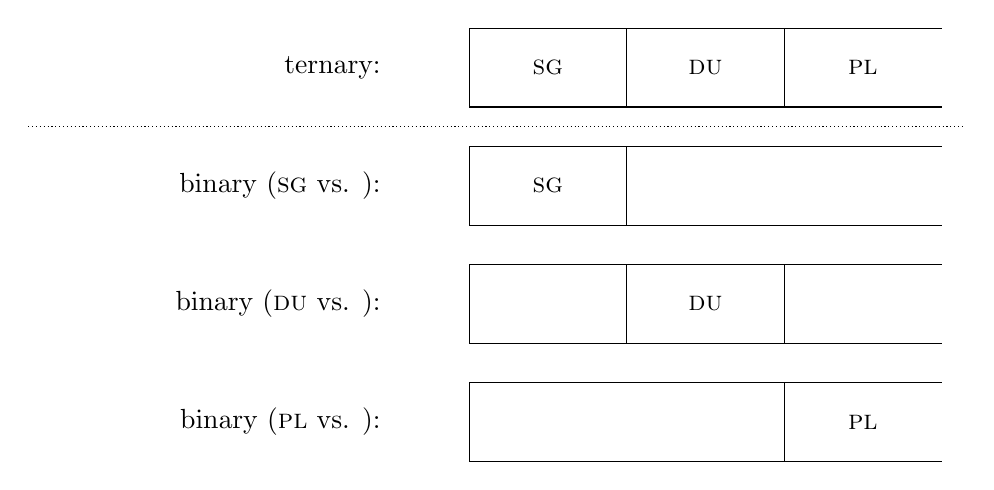
\begin{tikzpicture}
	\draw (1,4.5) --(7,4.5);
	\draw (1,5.5) --(7,5.5);
	\draw (1,4.5) --(1,5.5);
	\draw (3,4.5) --(3,5.5);
	\draw (5,4.5) --(5,5.5);
	\node at (2,5){\Sg};
	\node at (4,5){\Du};
	\node at (6,5){\Pl};
	\draw[densely dotted] (-4.6,4.25) --(7.3,4.25);
	\draw (1,3) --(7,3);
	\draw (1,4) --(7,4);
	\draw (1,3) --(1,4);
	\draw (3,3) --(3,4);
	\node at (2,3.5){\Sg};
	\node at (5,3.5){\Nsg};
	\draw (1,1.5) --(7,1.5);
	\draw (1,2.5) --(7,2.5);
	\draw (1,1.5) --(1,2.5);
	\draw (3,2) --(3,2.5);
	\draw (5,2) --(5,2.5);
	\draw (3,2) --(3,1.5);
	\draw (5,2) --(5,1.5);
	\node at (4,2){\Du};
	\node at (2,2){\Ndu};
	\node at (6,2){\Ndu};
	\draw (1,0) --(7,0);
	\draw (1,1) --(7,1);
	\draw (1,0) --(1,1);
	\draw (5,0) --(5,1);
	\node at (3,0.5){\Npl};
	\node at (6,0.5){\Pl};
	\node[left] at (0,5) {ternary:};
	\node[left] at (0,3.5) {binary (\Sg{} vs. \Nsg{}):};
	\node[left] at (0,2) {binary (\Du{} vs. \Ndu):};
	\node[left] at (0,0.5) {binary (\Pl{} vs. \Npl):};
\end{tikzpicture}
\caption{Three ways of breaking up a ternary opposition}\label{ternbinary}
\end{figure}%Three ways of breaking up a ternary opposition

Komnzo makes use of all three oppositions, but only two of the possible combinations. The \isi{person} affixes operate always on a \isi{singular} vs. \isi{non-singular} opposition. A separate affix, which I call the duality affix, makes a distinction between \isi{dual} vs. \isi{non-dual}. I will show below that under certain circumstances, the same affix encodes \isi{plural} vs. \isi{non-plural}, but this is a marginal pattern (\S{}\ref{prerootdual}). The basic system of distributed \isi{number} marking integrates a \Sg{}-\Nsg{} opposition in the \isi{person} affixes with a \Du-\Ndu{} opposition in the duality affix. Figure \ref{basicnumberm} provides an overview of this principle.

\begin{figure}

	\begin{tabularx}{\textwidth}{|c|c|p{1,5cm}p{1,5cm}|}
		\cline{3-4}
		\multicolumn{2}{c|}{}&\multicolumn{2}{c|}{\textsc{duality affix}}\\\cline{3-4}
		\multicolumn{2}{c|}{}&\multicolumn{1}{c}{\Du}&\multicolumn{1}{|c|}{\Ndu}\\
		\hline 
		\parbox[t]{2mm}{\multirow{6}{*}{\rotatebox[origin=c]{90}{\textsc{person affix}}}}&\parbox[t]{2mm}{\multirow{3}{*}{\rotatebox[origin=c]{90}{\Sg}}}&\multicolumn{1}{c}{\multirow{3}{*}{}}&\\
		&&&\multicolumn{1}{c|}{singular}\\
		&&&\\\cline{2-2}
		&\parbox[t]{2mm}{\multirow{3}{*}{\rotatebox[origin=c]{90}{\Nsg}}}&&\\
		&&\multicolumn{1}{c}{dual}&\multicolumn{1}{c|}{plural}\\
		&&&\\
		\hline
		\multicolumn{4}{c}{}\\
	\end{tabularx}
\caption{Basic principle of distributed number marking on verbs}\label{basicnumberm}
\end{figure}%Basic principle of distributed \isi{number} marking

Figure \ref{basicnumberm} shows that out of four possible combinations, in fact only three are normally put to use, namely those that are logically compatible. Prefixing verbs and stems in a prefixing template, which includes \isi{positional} verbs, are exceptional in that they utilise the fourth, seemingly non-sensical, combination \Sg{}-\Du{} to encode a \isi{large plural} (\S{}\ref{positonalnumber}).%\\

The two sites involved in \isi{number} marking have very different properties. The binary opposition in the \isi{person} prefixes and suffixes is much more stable in the sense that (i) the encoded value can be straightforwardly associated with an argument, because \isi{person} and \isi{number} marking are fused into one morpheme, (ii) the position of these affixes with respect to the stem is fixed and (iii) the values encoded are always \Sg{} and \Nsg{}. The duality affix differs in all three points and the subsequent discussion of \isi{number} marking will focus on its peculiarities. But to give an overview here: first, if there are two participants indexed in the verb, the duality affix is ambiguous as to which of the two it is indexing. Secondly, duality is marked in a suffix with extended stems, but in a complex \isi{portmanteau} prefix with restricted stems. Finally, as was mentioned above, in part of the paradigm, the \Du{}-\Ndu{} opposition is replaced by a \Pl{}-\Npl{} opposition. I will discuss these points below.

\subsubsection{Ambiguities in the reference of the duality affix} \label{ambiguitiesdualref}

Examples (\ref{ex215}-g) show the verb \emph{fathasi} `hold' with different \isi{number} combinations of the two arguments.\footnote{Note, that the \ili{English} translations are all in third person, although some of the person indexing morphemes neutralise the distinction between second and third person and, thus, could also be translated as second person.} Only in example (\ref{ex219}), we find several possibilities with respect to \isi{number} marking because both \isi{person} affixes signal \isi{non-singular}. The ambiguity stems from the fact that the duality marker is ambiguous as to which of the two arguments it is referencing. In other words, the \isi{dual} morpheme \emph{n-} in (\ref{ex219}) signals that one the two participants is \isi{dual}, but not which one. This does not create any ambiguities in cases where one of the the two \isi{person} affixes is \isi{singular} (\ref{ex215}-e). Likewise, it is not a problem if both \isi{person} affixes are \isi{non-singular} and the duality affix in \isi{non-dual} (\ref{ex220}). Although examples (\ref{ex215}-g) show the \isi{extended stem} of the verb \emph{fathasi}, this ambiguity is also found with restricted stems where the duality affix occurs in pre-stem position.

\begin{exe}
\ex
\begin{xlist}
	\ex
	\gll \emph{y-fath-wr-\Zero}\\
	\Tsg.\Masc-hold.\Ext-\Ndu-\Stsg\\
	\trans `S/He holds him.'
	\label{ex215}
	\ex
	\gll \emph{y-fath-n-th}\\
	\Tsg.\Masc-hold.\Ext-\Du-\Stnsg\\
	\trans `They (2) hold him.'
	\label{ex216}
	\ex
	\gll \emph{y-fath-wr-th}\\
	\Tsg.\Masc-hold.\Ext-\Ndu-\Stnsg\\
	\trans `They (3+) hold him.'
	\label{ex217}
	\ex
	\gll \emph{e-fath-n-\Zero}\\
	\Stnsg-hold.\Ext-\Du-\Stsg\\
	\trans `S/He holds them (2).'
	\label{ex218}
	\ex
	\gll \emph{e-fath-wr-\Zero}\\
	\Stnsg-hold.\Ext-\Ndu-\Stsg\\
	\trans `S/He holds them (3+).'
	\label{ex221}
	\ex
	\gll \emph{e-fath-n-th}\\
	\Stnsg-hold.\Ext-\Du-\Stnsg\\
	\trans `They (2) hold them (3+).' or `They (2) hold them (2).' or `They (3+) hold them (2).'
	\label{ex219}
	\ex
	\gll \emph{e-fath-wr-th}\\
	\Stnsg-hold.\Ext-\Ndu-\Stnsg\\
	\trans `They (3+) hold them (3+).'
	\label{ex220}
\end{xlist}
\end{exe}

For verbs in the \isi{transitive} ambifixing and \isi{ditransitive} ambifixing template, the distribution of the \isi{dual} and \isi{non-dual} markers can be expressed in an abstract way as in Figure \ref{dualitymatrixfathasi}.
\vspace{-.1cm}
\begin{figure}

	\begin{tabularx}{\textwidth}{|ccccccc|}
		\cline{3-5}
		\multicolumn{2}{c|}{}&\multicolumn{3}{c|}{\textsc{actor}}&\\\cline{3-5}
		\multicolumn{2}{c|}{}&\multicolumn{1}{c}{\Sg}&\multicolumn{1}{|c|}{\Du}&\multicolumn{1}{c|}{\Pl}&\\\cline{1-5}
		{\parbox[t]{2mm}{\multirow{6}{*}{\rotatebox[origin=l]{90}{\textsc{undergoer}\hspace{0,2cm}}}}}&\multicolumn{1}{|c|}{\parbox[t]{2mm}{\multirow{2}{*}{\rotatebox[origin=c]{90}{\Sg}}}}&\multicolumn{1}{c}{\multirow{2}{*}{\hspace{0,1cm}wr\hspace{0,1cm}}}	&\multirow{2}{*}{\hspace{0,1cm}n\hspace{0,1cm}}	&\multicolumn{1}{c|}{\multirow{2}{*}{\hspace{0,1cm}wr\hspace{0,1cm}}}&\\
		&\multicolumn{1}{|c|}{}&&&\multicolumn{1}{c|}{}\\\cline{2-2}
		&\multicolumn{1}{|c|}{\parbox[t]{2mm}{\multirow{2}{*}{\rotatebox[origin=c]{90}{\Du}}}}&\multicolumn{1}{c}{\multirow{2}{*}{\hspace{0,1cm}n\hspace{0,1cm}}}&\multirow{2}{*}{\hspace{0,1cm}n\hspace{0,1cm}}&\multicolumn{1}{c|}{\multirow{2}{*}{\hspace{0,1cm}n\hspace{0,1cm}}}&\\
		&\multicolumn{1}{|c|}{}&&&\multicolumn{1}{c|}{}\\\cline{2-2}
		&\multicolumn{1}{|c|}{\parbox[t]{2mm}{\multirow{2}{*}{\rotatebox[origin=c]{90}{\Pl}}}}&\multicolumn{1}{c}{\multirow{2}{*}{\hspace{0,1cm}wr\hspace{0,1cm}}}&\multirow{2}{*}{\hspace{0,1cm}n\hspace{0,1cm}}&\multicolumn{1}{c|}{\multirow{2}{*}{\hspace{0,1cm}wr\hspace{0,1cm}}}&\\
		&\multicolumn{1}{|c|}{}&&&\multicolumn{1}{c|}{}\\\cline{1-5}
	\end{tabularx}
\caption{The duality matrix with \emph{fathasi}}
\label{dualitymatrixfathasi}
\end{figure}%duality matrix post stem

For \isi{verb} forms which index only one argument the marking pattern is simpler, as there is no ambiguity in reference of the duality suffix. This is relevant for verbs in a prefixing or middle template. Examples (\ref{ex222}-c) show the verb \emph{thoraksi} `appear' in a prefixing template cycled through all three \isi{number} values.

\begin{exe}
\ex
\begin{xlist}
	\ex
	\gll \emph{wo-thorak-wr}\\
	\Fsg-appear.\Ext-\Ndu\\
	\trans `I arrive.'
	\label{ex222}
	\ex
	\gll \emph{n-thorak-n} ($\sim$ \emph{n-thorak-rn})\\
	\Fnsg-appear.\Ext-\Du{}\\
	\trans `We (2) arrive.'
	\label{ex223}
	\ex
	\gll \emph{n-thorak-wr}\\
	\Fnsg-appear.\Ext-\Ndu\\
	\trans `We (3+) arrive.'
	\label{ex224}
\end{xlist}
\end{exe}

Note that there are two variants for the \isi{dual} morpheme, \emph{-n} and \emph{-rn} in (\ref{ex223}), which are attested for almost all members of the small class of prefixing verbs. This variation is both intra-speaker and inter-speaker and, thus far, no patterning along social lines could be detected (e.g. age of the speaker, speaker's exposure to other varieties, etc).

\subsubsection{Large plurals with prefixing verbs} \label{positonalnumber}

The prefixing template indexes the sole argument of the \isi{verb} in the prefix, while the suffix slot is not used. We have seen that only a small number of verbs are inherently prefixing (\S{}\ref{prefixingverbsec}), and about fifty stems may enter into this template. The latter group includes \isi{positional} verbs (\S{}\ref{positionalverbs}). I show below that because there is no ambiguity in the reference of the duality marker, all four cells in the paradigm can be exploited. This allows for a fourth \isi{number} value, the \isi{large plural}, which is formed by combining the \isi{dual} marker with a \isi{singular}. Figure \ref{prefnumberm} illustrates the pattern.

\begin{figure}

	\begin{tabularx}{\textwidth}{|c|c|p{2cm}p{2cm}|}
		\cline{3-4}
		\multicolumn{2}{c|}{}&\multicolumn{2}{c|}{\textsc{duality affix}}\\\cline{3-4}
		\multicolumn{2}{c|}{}&\multicolumn{1}{c}{\Du}&\multicolumn{1}{|c|}{\Ndu}\\
		\hline
		\parbox[t]{2mm}{\multirow{6}{*}{\rotatebox[origin=c]{90}{\textsc{person affix}}}}&\parbox[t]{2mm}{\multirow{3}{*}{\rotatebox[origin=c]{90}{\Sg}}}&\multicolumn{1}{c}{\multirow{3}{*}{}}&\\
		&&\multicolumn{1}{c}{large plural}&\multicolumn{1}{c|}{singular}\\
		&&&\\ \cline{2-2}
		&\parbox[t]{2mm}{\multirow{3}{*}{\rotatebox[origin=c]{90}{\Nsg}}}&&\\
		&&\multicolumn{1}{c}{dual}&\multicolumn{1}{c|}{plural}\\
		&&&\\ 
		\hline
		\multicolumn{4}{c}{}\\
	\end{tabularx}
\caption{Principle of distributed number marking for prefixing verbs}
\label{prefnumberm}
\end{figure}%prefixing verb and large plurals

Consider example (\ref{ex715}) below. The speaker in the story has been away from Rouku for a long time. He asks his brother whether the palm wine containers are still hanging, and the brother replies `there are plenty'. This is expressed by the copula in \isi{dual} and the prefix in \isi{singular}. Note that the stem of the copula is sensitive to \isi{dual} versus \isi{non-dual}. I used the \isi{gloss} label \Lpl{} for \isi{large plural}.

\begin{exe}
	\ex \emph{``eh ngthé bana! sgeru komnzo emithgr?'' ``ah, segeru komnzo \textbf{yrn}''}\\
	\glll eh ngthé bana sgeru komnzo e-mi-thgr ah\\
	hey {brother} poor {palm.wine} still \Stnsg:\Alph-hang.\Ext-\Stat.\Ndu{} ah\\
	{} {} {} {} {} \footnotesize{\Stpl:\Sbj:\Nonpast:\Stat/hang} {}\\
	\sn
	\glll segeru komnzo y-rn\\
	{palm.wine} still \Tsg.\Masc:\Alph-\Cop.\Du\\
	{} {} \footnotesize{\Third\Lpl:\Sbj:\Nonpast:\Ipfv/be}\\
	\trans ``Hey brother, are the palm wine (containers) still hanging?'' ``Yes, there are still plenty.'' \Corpus{tci20130927-06}{MAB \#189}
	\label{ex715}
\end{exe}

Examples (\ref{ex225}-d) are elicited forms showing the \isi{positional} verb \emph{räzsi} `erect, stand up' in all four \isi{number} values.\footnote{Note that we find the same variation in the dual morpheme (\emph{-n} and \emph{-rn}) as with other prefixing verbs. Compare with examples \ref{ex222}-c above.}

\begin{exe}
\ex
\begin{xlist}
	\ex
	\gll \emph{woz} \emph{w-räs-thg-r}\\
	bottle \Tsg.\F-erect-\Stat-\Ndu\\
	\trans `The bottle is standing.'
	\label{ex225}
	\ex
	\gll \emph{woz} \emph{e-räs-thg-n} ($\sim$ \emph{e-räs-thg-rn})\\
	bottle \Stnsg-erect-\Stat-\Du\\
	\trans `The two bottles are standing.'
	\label{ex226}
	\ex
	\gll \emph{woz} \emph{e-räs-thg-r}\\
	bottle \Stnsg-erect-\Stat-\Ndu\\
	\trans `The bottles are standing.'
	\label{ex227}
	\ex
	\gll \emph{woz} \emph{y-räs-thg-n} ($\sim$ \emph{y-räs-thg-rn})\\
	bottle \Tsg.\Masc-erect-\Stat-\Du\\
	\trans `All the bottles are standing.' or `Many bottles are standing.'
	\label{ex228}
\end{xlist}
\end{exe}

Example (\ref{ex228}) shows the \isi{large plural} construction in which the seemingly non-sensical combination of a \isi{singular} in the \isi{person} prefix and a \isi{dual} in the duality slot yields a \isi{large plural} or exhaustive \isi{plural} interpretation. There are some restrictions to the large pural. First, as we have seen, it only occurs in the prefixing template. Even though a stem like \emph{räz-} `erect' can appear in a middle or ambifixing template, it cannot form large plurals in these templates. Secondly, large plurals only occur in third \isi{person}, not in first or second. Note that it is always the \isi{masculine} prefix which is used in the \isi{large plural} construction, even if the referent is \isi{feminine}, as with \emph{woz} `bottle' (\ref{ex225}). In this way, the \isi{large plural} construction substantiates the principle of \isi{distributed exponence}, whereby the morphological material at the language's disposal is employed in ways that are not predictable by looking at individual morphemes.%\\

Unfortunately, the \isi{large plural} construction is attested only once in the corpus (\ref{ex715}). The evidence presented above comes from eliciation.\footnote{I want to thank Nick Evans for pointing out the combinatorial possibility (\Sg+\Du) in \ili{Nen} (\citealt{Evans:2014bz}) which allowed me to test this pattern with Komnzo speakers.} Although the \isi{large plural} is readily understood and judged grammatical by all my informants, I have not overheard it in daily conversation. Speakers commonly refer to this construction as `a way the old people spoke'. Therefore, we have to assume that it will fade from the speakers' \isi{passive} knowledge eventually and disappear altogether. In fact, the speaker in example (\ref{ex715}) was an older man.%\\

Although on different levels of comparison, \isi{dual} marking in pre-stem position and the formation of large plurals are not compatible. This is partly caused by the \isi{stative} semantics of verbs in the prefixing template. For example, positionals take the \isi{stative} suffix \emph{-thgr} which blocks all \isi{perfective} semantics. Pre-stem \isi{dual} marking on the other hand occurs only with restricted stems, and restricted stems are used to form perfectives. A \isi{positional} verb like \emph{räzsi} `erect', can occur outside the prefixing template and form perfectives, but in this case the \isi{large plural} does not apply. We saw in \S{}\ref{prefixingverbsec}, that there are some prefixing verbs, which are not \isi{stative}, for example \emph{yarenzsi} `look around' or \emph{ziksi} `turn to side'. These do form perfectives in the prefixing template. However, the \isi{large plural} combination results in an ungrammatical inflection.%\\

I suggest that a historical perspective explains why this is the case. I show in \S{}\ref{prerootdual}, that pre-stem \isi{dual} marking is messier than post-stem \isi{dual} marking in the sense that it is less segmentable and there are more patterns of syncretism. I have argued in \S{}\ref{comparativenoteextrs} that pre-stem \isi{dual} marking is an innovation, and that post-stem \isi{dual} marking is an older pattern. Thus, the \isi{large plural} construction has not survived the change in the pattern shift. Therefore, prefixing verbs with dynamic semantics cannot form large plurals in their perfectives.

\subsubsection{Allomorphy in the post-stem duality slot} \label{allomorphdualsuffix}

Before I turn to the \isi{dual} marking in pre-stem position with restricted stems, I discuss the topic of allomorphy in post-stem position. The \isi{dual} morpheme in the duality slot shows little variation. The above described variation between \emph{-n} and \emph{-rn} is found with prefixing verbs only; elsewhere the \isi{dual} morpheme is always \emph{-n}. As for the \isi{non-dual} morpheme, the situation is different. There are three allomorphs (\emph{wr-}, \emph{nzr-}, \emph{-r}) and their distribution is phonologically conditioned by the final element of the verb stem. The conditioning rules layed out in Table \ref{allonondual} account for 85\% (275/322) of the attested \isi{verb} lexemes.

\begin{table}
	\caption{Allomorphs of the non-dual suffix}
\begin{tabularx}{\textwidth}{XXrXl}
	\label{allonondual}\\
	\lsptoprule
	{formatives} & {rule} &{count}& {\textsc{example}}& {gloss}\\
	\midrule
	%\endfirsthead
	{formative} & {rule} &{count}& {\textsc{example}}& {gloss}\\
	\midrule
	%\endhead
	\emph{-wr}& / k]\textsubscript{\tiny{stem}}\_&92& \emph{mätrak-}& `bring out'\\
	&&& \emph{wek-}&`invite'\\
	& / g]\textsubscript{\tiny{stem}}\_	&38& \emph{mäyog-}& `repeat'\\
	&&& \emph{brig-}&`return'\\
	& / n]\textsubscript{\tiny{stem}}\_	&34& \emph{wathkn-}& `pack up'\\
	&&& \emph{myukn-}&`twist'\\
	& / r]\textsubscript{\tiny{stem}}\_	&25& \emph{rsr-}& `fish (poison)'\\
	&&& \emph{wagr-}&`meet'\\\midrule
	\emph{-nzr}	& / V]\textsubscript{\tiny{stem}}\_&62& \emph{yagu-}& `pour out'\\
	&&& \emph{yafü-}& `open'\\
	&&& \emph{mrä-}& `stroll'\\
	&&& \emph{fsi-}& `count'\\
	&&& \emph{tha-}& `uncover'\\\midrule
	\emph{-r}& / z]\textsubscript{\tiny{stem}}\_&24& \emph{brüz-}& `submerge'\\
	&&& \emph{rifthz-}& `hide'\\
	&&& \emph{räz-}& `erect'\\\midrule
	\textsc{total}&&275&&\\
	\lspbottomrule
\end{tabularx}%Allomorphs of the \isi{non-dual} suffix
\end{table}


The remaining 15\% of \isi{verb} lexemes are irregular (i) in taking a different formative to mark \isi{non-dual} (e.g. \emph{-thr} or \emph{-\Zero}), (ii) in taking one of the three allomorphs under violation of the conditioning rules or (iii) in expressing the \isi{dual}/\isi{non-dual} contrast by irregular changes in the verb stem, for example \emph{moth} `walk' (\emph{-yak} \Ndu{} vs. \emph{-yan} \Du) or \emph{kwan} `shout' (\emph{-nor} \Ndu{} vs. \emph{-rn} \Du).

\subsubsection{Pre-stem dual marking with restricted stems} \label{prerootdual}

The previous discussion concentrated on \isi{dual} marking with extended stems. For restricted stems, this suffix slot is not available and the \isi{dual} vs. \isi{non-dual} contrast is marked in the vowel of the prefix, which changes to \emph{ä} for \isi{non-dual}. Pre-stem \isi{dual} marking is relevant only for those TAM categories which build their inflection on the \isi{restricted stem}. These are verbs inflected for \isi{iterative} and \isi{perfective} \isi{aspect}. The latter include indicative (\isi{recent past} and \isi{past} \isi{tense}), \isi{imperative} or \isi{irrealis} forms. In the following description, I use the \isi{irrealis} \isi{perfective} forms to explain the pattern and point to other TAM categories where they deviate.%\\

Interestingly, it is the \isi{non-dual} that receives a marker (\emph{ä-}), while the \isi{dual} is \isi{zero} marked. At the same time, pre-stem \isi{dual} marking is less segmentable and harder to \isi{gloss} than post-stem \isi{dual} marking, because the \isi{non-dual} \emph{ä} vowel superposes vowels from other prefixal material, for example the \isi{valency} changer \emph{a-} or the \isi{irrealis} prefix \emph{ra-}. This leads to patterns of syncretism which span several grammatical dimensions (\isi{valency}, \isi{number}, \isi{aspect}, \isi{mood}, etc).%\\

Ir\isi{realis} mood is expressed by the prefix \emph{ra-}, which directly follows the \isi{person}/\isi{number} prefix or the middle marker of the \Bet{} \isi{prefix series} (see Table \ref{perspref} in \S{}\ref{personprefsection}). The \isi{non-dual} marker \emph{ä} replaces the vowel of the \emph{ra-} prefix for all the \isi{person}/\isi{number} combinations which involve a \isi{non-dual} \isi{participant}. This pattern is uniform for prefixing as well as ambifixing verbs. Below in (\ref{ex243}-\ref{ex247}), I provide textual examples of the \isi{number} combinations with a third \isi{person} actor and a first \isi{person} \isi{undergoer}.\footnote{Irrealis mood may be used in narratives for pragmatic reasons (backgrounding) and refer to events which actually took place (\S{}\ref{TAMsemmood})} We find the \emph{ä} vowel for the following actor>undergoer combinations: \Sg>\Sg{} (\ref{ex243}), \Pl>\Sg{} (\ref{ex246}), \Sg>\Pl{} (\ref{ex249}) and \Pl>\Pl{} (\ref{ex250}).

\begin{exe}
	\ex \emph{adif nima \textbf{kwräs} ``ranzo?''}\\
	\glll adi=f nima kw-rä-s-\Zero{} ra=nzo\\
	aunt=\Erg.\Sg{} \Quot{} \Fsg.\Bet-\Irr.\Ndu-ask.\Rs-\Stsg{} what=\Only\\
	{} {} \footnotesize{\Stsg:\Sbj>\Fsg:\Obj:\Irr:\Pfv/ask} {}\\
	\trans `Aunt asked me: ``What is it?''' \Corpus{tci20120922-25}{ALK \#15-16}
	\label{ex243}
\end{exe}
\begin{exe}
	\ex \emph{yare kma nzä nafa \textbf{kwrakarth}.}\\
	\glll yare kma nzä nafa kw-ra-kar-th\\
	bag \Pot{} \Fsg.\Abs{} \Tnsg.\Erg{} \Fsg.\Bet-\Irr.\Du-pull.\Rs-\Stnsg\\
	{} {} {} {} \footnotesize{\Stdu:\Sbj>\Fsg:\Obj:\Irr:\Pfv/pull}\\
	\trans `They (2) should take the bag from me.' \Corpus{tci20130907-02}{JAA \#10}
	\label{ex245}
\end{exe}
\begin{exe}
	\ex \emph{ngatha fäth ferä nafa \textbf{kwränbrmth} e ...}\\
	\glll ngatha fäth f=e-rä nafa\\
	dog \Dim{} \Dist=\Stnsg.\Alph-\Cop.\Ndu{} \Tnsg.\Erg{}\\
	{} {} \footnotesize{\Dist=\Stpl:\Sbj:\Nonpast/be} {}\\
	\sn
	\glll kw-rä-n-brm-th e (.)\\
	\Fsg{}.\Bet{}-\Irr.\Ndu-\Venit-follow.\Rs-\Stnsg{} until (.)\\
	\footnotesize{\Stpl:\Sbj>\Fsg:\Obj:\Irr:\Pfv:\Venit/follow} {} {}\\
	\trans `The small dogs over there, they follow me until...' \Corpus{tci20111119-03}{ABB \#94}
	\label{ex246}
\end{exe}
\begin{exe}
	\ex \emph{foba \textbf{nzrans} ``bä mon ern?''}\\
	\glll foba nz-ra-n-s-\Zero{} bä mon e-rn\\
	\Dist.\Abl{} \Fnsg.\Bet-\Irr.\Du-\Venit-ask.\Rs-\Stsg{} \Second.\Abs{} how \Stnsg.\Alph-\Cop.\Du\\
	{} \footnotesize{\Stsg:\Sbj>\Fdu:\Obj:\Irr:\Pfv:\Venit/ask} {} {} \footnotesize{\Stdu:\Sbj:\Nonpast:\Ipfv/be}\\
	\trans `He asked us (2): ``Who are you?''' \Corpus{tci20120904-02}{MAB \#125}
	\label{ex248}
\end{exe}
\begin{exe}
	\ex \emph{paituaf \textbf{nzräkor} ``nzä fiyafr wiyak.''}\\
	\glll paitua=f nz-rä-kor-\Zero{} nzä fiyaf=r\\
	old.man=\Erg.\Sg{} \Fnsg.\Bet-\Irr.\Ndu-speak.\Rs-\Stsg{} \Fsg.\Abs{} hunting=\Purp{}\\
	{} \footnotesize{\Stsg:\Sbj>\Fpl:\Obj:\Irr:\Pfv/speak} {} {}\\
	\sn
	\glll wo-yak\\
	\Fsg.\Alph-walk.\Ext.\Ndu\\
	\footnotesize{\Fsg:\Nonpast:\Ipfv/walk}\\
	\trans `He said to us: ``I will go hunting.''' \Corpus{tci20120821-02}{LNA \#11-12}
	\label{ex249}
\end{exe}
\begin{exe}
	\ex \emph{kar zf rä zf masu ... manema \textbf{nzräkorth} masu kar.}\\
	\glll kar zf rä zf masu (.) mane=ma\\
	place \Imm{} \Tsg.\F.\Cop.\Ndu{} \Imm{} masu (.) which=\Char{}\\
	{} {} \footnotesize{\Tsg.\F:\Sbj:\Nonpast.\Ipfv/be} {} {} {} {}\\
	\sn
	\glll
	nz-rä-kor-th masu kar\\
	\Fnsg.\Bet-\Irr.\Ndu-speak.\Rs-\Stnsg{} masu place.\\
	\footnotesize{\Stpl:\Sbj>\Fpl:\Obj:\Irr:\Pfv/speak} {} {}\\
	\trans `This place right here is Masu, which is why they call us Masu people.'\\ \Corpus{tci20120922-08}{DAK \#87}
	\label{ex250}
\end{exe}
\begin{exe}
	\ex \emph{ni \textbf{nzrakorth} ``bä!'' ... oroman babua ... ``bä kwa ŋakwinth zmbär aki kwayanen!''}\\
	\glll ni nz-ra-kor-th bä (.) oroman babua (.) bä kwa\hspace*{2cm} ŋ-a-kwi-n-th zmbär aki kwayan=en\\
	\Fnsg{} \Fnsg.\Bet-\Irr.\Du-speak.\Rs-\Stnsg{} \Second.\Abs{} (.) old.man babua (.) \Second.\Abs{} \Fut{} \M.\Alph-\Vc-run.\Ext-\Du-\Stnsg{} night moon light=\Loc\\
	{} \footnotesize{\Stpl:\Sbj>\Fdu:\Obj:\Irr:\Pfv/speak} {} {} {} {} {} {} {} \footnotesize{\Stdu:\Sbj:\Nonpast:\Ipfv/run} {} {} {}\\
	\trans `They said to us (2): ``You!'' to old man Babua ``You two will run at night in the moonlight''' \Corpus{tci20120904-01}{MAB \#135-137}
	\label{ex247}
\end{exe}

Note that just like in post-stem \isi{dual} marking (\S{}\ref{ambiguitiesdualref}), pre-stem \isi{dual} marking is ambiguous as to which of the two arguments is \isi{dual} or \isi{non-dual}. The verb \emph{nzrakorth} `they said to us' in (\ref{ex247}) could be any of the three possible actor>\isi{undergoer} combinations (\Pl>\Du, \Du>\Du{} or \Du>\Pl) because both \isi{person} affixes index a \isi{non-singular} \isi{participant}. Thus, the absence of the \emph{ä} vowel indicates that one of the two participants is \isi{dual}, but not which one. Only context may solve this structural ambiguity, which in (\ref{ex247}) is clear from the second verb \emph{ŋakwinth} `you two go'. For verbs in a prefixing template, there is no ambiguity since they index only one argument. Non-\isi{dual} participants receive the \emph{ä} vowel, while \isi{dual} participants do not. The same holds for verbs in the middle template.%\\

The marking pattern can be expressed in an abstract matrix as in Figure \ref{raezerorae}. In terms of structure, not in its formatives, this matrix is identical to post-stem duality marking (see Figure \ref{dualitymatrixfathasi} above).

\begin{figure}

	\begin{tabularx}{\textwidth}{|ccccccc|}
		\cline{3-5}
		\multicolumn{2}{c|}{}&\multicolumn{3}{c|}{\textsc{actor}}&\\\cline{3-5}
		\multicolumn{2}{c|}{}&\multicolumn{1}{c}{\Sg}&\multicolumn{1}{|c|}{\Du}&\multicolumn{1}{c|}{\Pl}&\\\cline{1-5}
		{\parbox[t]{2mm}{\multirow{6}{*}{\rotatebox[origin=l]{90}{\textsc{undergoer}\hspace{0,1cm}}}}}&\multicolumn{1}{|c|}{\parbox[t]{2mm}{\multirow{2}{*}{\rotatebox[origin=c]{90}{\Sg}}}}&\multicolumn{1}{c}{\multirow{2}{*}{\hspace{0,1cm}ä\hspace{0,1cm}}}&\multirow{2}{*}{\hspace{0,1cm}\Zero{}\hspace{0,1cm}}	&\multicolumn{1}{c|}{\multirow{2}{*}{\hspace{0,1cm}ä{\hspace{0,1cm}}}}&\\
		&\multicolumn{1}{|c|}{}&&&\multicolumn{1}{c|}{}\\\cline{2-2}
		&\multicolumn{1}{|c|}{\parbox[t]{2mm}{\multirow{2}{*}{\rotatebox[origin=c]{90}{\Du}}}}&\multicolumn{1}{c}{\multirow{2}{*}{\hspace{0,1cm}\Zero{}\hspace{0,1cm}}}&\multirow{2}{*}{\hspace{0,1cm}\Zero{}\hspace{0,1cm}}&\multicolumn{1}{c|}{\multirow{2}{*}{\hspace{0,1cm}\Zero{}\hspace{0,1cm}}}&\\
		&\multicolumn{1}{|c|}{}&&&\multicolumn{1}{c|}{}\\\cline{2-2}
		&\multicolumn{1}{|c|}{\parbox[t]{2mm}{\multirow{2}{*}{\rotatebox[origin=c]{90}{\Pl}}}}&\multicolumn{1}{c}{\multirow{2}{*}{\hspace{0,1cm}ä\hspace{0,1cm}}}&\multirow{2}{*}{\hspace{0,1cm}\Zero{}\hspace{0,1cm}}&\multicolumn{1}{c|}{\multirow{2}{*}{\hspace{0,1cm}ä\hspace{0,1cm}}}&\\
		&\multicolumn{1}{|c|}{}&&&\multicolumn{1}{c|}{}\\\cline{1-5}
	\end{tabularx}
\caption{The duality matrix without \Vc{} prefix}
\label{raezerorae}
\end{figure}%duality matrix without VC

There are some exceptions for the third singular prefixes (both feminine and masculine). The combination of \Sg>\Tsg{} in the ambifixing template and \Tsg{} in the prefixing template receive the vowel \emph{a} and not \emph{ä} in all relevant TAM categories. In the imperatives, it is \emph{a} for both combinations \Sg>\Tsg{} and \Pl>\Tsg{}. Inflections involving a \isi{dual} \isi{participant} would receive a \isi{zero} marker. In a discussion after listening to old recordings made by the anthropologist Mary Ayres in the 1980's, I was able to elicit one inflectional form that is relevant to this topic. The informant contrasted the modern Komnzo inflection \emph{santhor} `He arrived here' with an older form of the same verb \emph{snäthor}.\footnote{\parbox{0.02cm}{\hfill}\parbox{6cm}{\emph{s-a-n-thor}} \parbox{5cm}{\emph{s-n-ä-thor}}\\ \parbox{0.1cm}{\hfill}\parbox{6cm}{\Tsg.\Masc.\Gam-\Ndu-\Venit-arrive.\Rs{}}  \parbox{15cm}{\Tsg.\Masc.\Gam-\Venit-\Ndu-arrive.\Rs}} A first observation is that the \emph{ä} does occur in the older form. Interestingly, it occurs after the \isi{ventive} \emph{n-} prefix. At the current stage of documentation, not much can be said about the time frame during which this change has occured. The informant who provided this information is now in his mid-60's and he remembers `old people' using this form. I was not able to elicit a full paradigm of these older inflections and, thus, we are denied insight into the changes that took place in the verb template. As for now, we can only state that the \isi{non-dual} \emph{ä} vowel existed at some point in time with third singulars in the prefix.%\\

As I mentioned above, since pre-stem duality marking involves the \emph{ä} vowel, it occupies a slot in the template which may be filled by other prefixal material, for example the irrealis prefix \emph{ra-} and the \isi{valency} changer \emph{a-}, or both. We saw in the examples above, that the \isi{non-dual} \emph{ä} vowel superposes the irrealis \emph{ra-} prefix which results in the form \emph{rä-}. This is not the case for the imperatives and indicative inflected verbs. As we have seen in \S{}\ref{combinatoricsextrs}, restricted stems combine only with prefixes of the \Bet{}, \Betatwo{} and \Gam{} series. Most formatives of these series are composed of only a consonant (See Table \ref{perspref} in \S{}\ref{personprefsection}). Only the \Fsg.\Gam{} (\emph{zu-}) and all formatives of the \Betatwo{} series end in /u/, which resyllabifies as part of a complex onset (\emph{zw-}) in the presence of \emph{ä} or \emph{a}. For example, the \Fsg.\Gam{} \emph{zu-} in (\ref{ex258}) is followed by a \isi{zero}. Therefore, the verb is inflected for \isi{dual}. In (\ref{ex257}), the \Fsg.\Gam{} is followed by the \isi{non-dual} \emph{ä} vowel and the prefix changes into \emph{zwä-}. Therefore, I analyse the distribution of the \emph{ä} vowel as was shown above in Figure \ref{raezerorae}.

\begin{exe}
	\ex \emph{nzä nima \textbf{zukorth}: ``be fafä zane nagayé fäth zä thamonegwé!''}\\
	\glll nzä nima zu-\Zero-kor-th be fafä zane\\
	\Fsg.\Abs{} \Quot{} \Fsg.\Gam-\Du-speak.\Rs-\Stnsg{} \Ssg.\Erg{} after.this \Dem:\Prox{}\\
	{} {} \footnotesize{\Stdu:\Sbj>\Fsg:\Obj:\Rpst:\Pfv/speak} {} {} {}\\
	\sn
	\glll nagayé fäth zä th-a-moneg-w-é\\
	children \Dim{} \Prox{} \Stnsg.\Bet-\Vc-wait.\Ext-\Ndu-\Ssg.\Imp{}\\
	{} {} {} \footnotesize{\Ssg:\Sbj>\Stpl:\Io:\Imp:\Ipfv/wait}\\
	\trans `They (2) said to me: ``You will look after these small children here later!'''\\ \Corpus{tci20121019-04}{ABB \#97}
	\label{ex258}
\end{exe}
\begin{exe}
	\ex \emph{watik, naf \textbf{zwäkora}: ``watik, nzone efoth fof \hspace*{2cm} zefafth.''}\\
	\glll watik naf zu-ä-kor-a-\Zero{} watik nzone efoth fof z-ä-faf-th\\
	then \Tsg.\Erg{} \Fsg.\Gam-\Ndu-speak.\Rs-\Pst-\Stsg{} then \Fsg.\Poss{} sun|day \Emph{} \M.\Gam-\Ndu.\Vc-hold.\Rs-\Stnsg{}\\
	{} {} \footnotesize{\Stsg:\Sbj>\Fsg:\Obj:\Pst:\Pfv/speak} {} {} {} {} \footnotesize{\Stnsg:\Sbj:\Pst:\Pfv/hold}\\
	\trans `Then she said to me: ``Well, my days are over now.''' \Corpus{tci20130911-03}{MBR \#76}
	\label{ex257}
\end{exe}

Pre-stem duality marking co-occurs with the \isi{valency change} prefix \emph{a-}. The resulting vowel pattern is summarised in the matrix in Figure \ref{raezeroraevalchange}, which shows that the \isi{non-dual} \emph{ä} vowel (i) replaces the \emph{a-} prefix and (ii) that it patterns differently to the forms given so far. Compare Figure \ref{raezerorae} above with Figure \ref{raezeroraevalchange} below. Note that this neutralises the \isi{valency change} prefix \emph{a-} for some of the actor>\isi{undergoer} combinations: \Pl>\Sg{}, \Sg>\Pl{} and \Pl>\Pl{}. For these combinations, it is only the \isi{case} frame which identifies whether the \isi{undergoer} argument is a direct \isi{object} (\Abs{} \isi{case}) or an indirect object (\Dat{} or \Poss{} \isi{case}).

\begin{figure}

	\begin{tabularx}{\textwidth}{|ccccccc|}
		\cline{3-5}
		\multicolumn{2}{c|}{}&\multicolumn{3}{c|}{\textsc{actor}}&\\\cline{3-5}
		\multicolumn{2}{c|}{}&\multicolumn{1}{c}{\Sg}&\multicolumn{1}{|c|}{\Du}&\multicolumn{1}{c|}{\Pl}&\\\cline{1-5}
		{\parbox[t]{2mm}{\multirow{6}{*}{\rotatebox[origin=l]{90}{\textsc{undergoer}\hspace{0,15cm}}}}}&\multicolumn{1}{|c|}{\parbox[t]{2mm}{\multirow{2}{*}{\rotatebox[origin=c]{90}{\Sg}}}}&\multicolumn{1}{c}{\multirow{2}{*}{\hspace{0,15cm}a\hspace{0,15cm}}}	&\multirow{2}{*}{\hspace{0,15cm}a\hspace{0,15cm}}	&\multicolumn{1}{c|}{\multirow{2}{*}{\hspace{0,15cm}ä\hspace{0,15cm}}}&\\
		&\multicolumn{1}{|c|}{}&&&\multicolumn{1}{c|}{}\\\cline{2-2}
		&\multicolumn{1}{|c|}{\parbox[t]{2mm}{\multirow{2}{*}{\rotatebox[origin=c]{90}{\Du}}}}&\multicolumn{1}{c}{\multirow{2}{*}{\hspace{0,15cm}a\hspace{0,15cm}}}&\multirow{2}{*}{\hspace{0,15cm}a\hspace{0,15cm}}&\multicolumn{1}{c|}{\multirow{2}{*}{\hspace{0,15cm}a\hspace{0,15cm}}}&\\
		&\multicolumn{1}{|c|}{}&&&\multicolumn{1}{c|}{}\\\cline{2-2}
		&\multicolumn{1}{|c|}{\parbox[t]{2mm}{\multirow{2}{*}{\rotatebox[origin=c]{90}{\Pl}}}}&\multicolumn{1}{c}{\multirow{2}{*}{\hspace{0,15cm}ä\hspace{0,15cm}}}&\multirow{2}{*}{\hspace{0,15cm}a\hspace{0,15cm}}&\multicolumn{1}{c|}{\multirow{2}{*}{\hspace{0,15cm}ä\hspace{0,15cm}}}&\\
		&\multicolumn{1}{|c|}{}&&&\multicolumn{1}{c|}{}\\\cline{1-5}
	\end{tabularx}
\caption{The duality matrix with \Vc{} prefix}
\label{raezeroraevalchange}
\end{figure}%duality matrix with VC

One exception is the combination of \Sg>\Sg{}. As we can see in Figure \ref{raezeroraevalchange}, this combination receives no \emph{ä} vowel although both participants are \isi{non-dual}. This pattern is regular for all persons. Thus, a \Pl>\Tsg{} would receive \emph{ä}, whereas \Du>\Tsg{} and \Sg>\Tsg{} would not receive it. For the last combination and all prefixing verbs with a \Tsg{} this means that the \isi{valency change} is neutralised and again only the \isi{case} frame shows what type of \isi{undergoer} is indexed. It is not neutralised for the other \isi{person} values (\Sg>\Fsg{}, \Sg>\Ssg{} and \Fsg{}, \Ssg{} on prefixing verbs) precisely because \Sg>\Sg{} (and the \Sg{} in prefixing verbs) does not take \emph{ä} but \emph{a}.%\\

Note that prefixing verbs with the \isi{valency change} prefix \emph{a-} show a pattern where \emph{ä} only occurs on a \isi{plural}, while \emph{a} occurs with a singular and \isi{dual} \isi{participant}. At least on the surface, this results in the binary opposition of \isi{plural} vs. \isi{non-plural}. In (\ref{ex259}) below, the prefixing verb \emph{rfiksi} `grow' occurs in the inflected form \emph{zarfif} `sth. grew for/over it'. From the context, it is clear that the speaker is talking about the grass growing over the path. The verb encodes a \isi{feminine} \isi{undergoer}, which can only be interpreted as being the pathway (\emph{moth}), because \emph{yusi} `grass' is masculine. A \isi{dual} number of the \isi{undergoer} would be \emph{tharfif} and a \isi{plural} \emph{thärfif}. Thus, under several conditions (presence of \isi{valency change}, prefixing template, \isi{restricted stem}), the duality marker marks an opposition between \isi{plural} and \isi{non-plural}.

\begin{exe}
	\ex \emph{gathagatha moth rä ... z wrfrwake we ane \textbf{zarfif}.}\\
	\glll {gathagatha} moth rä (.) z\\
	bad path \Tsg.\F:\Cop:\Ndu{} (.) \Iam{}\\
	{} {} \footnotesize{\Tsg.\F:\Sbj:\Nonpast:\Ipfv/be} {} {}\\
	\sn
	\glll w-rfr-w-a-k-e we ane z-a-rfif\\
	\Tsg.\F.\Alph-trim.\Ext-\Ndu-\Pst-\Lk-\Fnsg{} also \Dem{} \Tsg.\F.\Gam-\Ndu.\Vc-grow.\Rs\\
	\footnotesize{\Fpl:\Sbj>\Tsg.\F:\Obj:\Pst:\Ipfv/trim} {} {} \footnotesize{\Tsg.\F:\Io:\Rpst:\Pfv/grow}\\
	\trans `This is a bad path. We cut it already, but (the grass) grew over it again.'\\ \Corpus{tci20130907-02}{RNA \#39-41}
	\label{ex259}
\end{exe}

Before I conclude this section on \isi{number} marking, I want to look at the behaviour of the \emph{ä} vowel when the \isi{irrealis} prefix \emph{ra-} and \isi{valency change} prefix \emph{a-} come together. Since the \isi{irrealis} prefix includes a vowel, the \isi{valency change} prefix is neutralised in most parts of the paradigm. For extended stems, this \isi{neutralisation} is complete, i.e. only the \isi{case} frame indicates whether the \isi{undergoer} argument is a direct \isi{object} (\Abs{}) or an \isi{indirect object} (\Dat{} or \Poss{}). This will be further discussed in \S{}\ref{irrealisra}. For restricted stems, the \isi{valency change} prefix \emph{a-} is likewise neutralised, but the \isi{number} marking pattern differs in those actor>\isi{undergoer} combinations which involve \Sg>\Sg{} (Figure \ref{raezeroraevalchange}). Consider the vowel contrast between (\ref{ex243}) which was given above and (\ref{ex251}) below. The \isi{participant} combination is held constant: \Tsg>\Fsg{}. In (\ref{ex243}) we find the \emph{ä} vowel, because it is \isi{ditransitive} and the \isi{valency change} prefix \emph{a-} is employed, but in (\ref{ex251}) it is missing, because (\ref{ex243}) is \isi{transitive} and lacks the \emph{a-} prefix. Compare (\ref{ex251}) with (\ref{ex252}) where the same verb \emph{yarisi} `give' shows the \emph{ä} because the actor \isi{participant} is \isi{plural}.

\begin{exe}
	\ex \emph{nafane bärbärnzo keke \textbf{kwrar}.}\\
	\glll nafane {bärbär=nzo} keke kw-ra-r-\Zero\\
	\Tsg.\Poss{} {half=\Only} \Neg{} \Fsg.\Bet{}-\Irr.\Ndu.\Vc-give.\Rs-\Stsg\\
	{} {} {} \footnotesize{\Stsg:\Sbj>\Fsg:\Io:\Irr:\Pfv/give}\\
	\trans `She will not give me half of her (fish).' \Corpus{tci20120922-26}{DAK \#125}
	\label{ex251}
\end{exe}
\begin{exe}
	\ex \emph{nä kwot \textbf{kwrärth} fafä.}\\
	\glll nä kwot kw-rä-r-th fafä\\
	some again \Fsg.\Bet-\Irr.\Pl.\Vc-give.\Rs-\Stnsg{} after.that\\
	{} {} \footnotesize{\Stpl:\Sbj>\Fsg:\Io:\Irr:\Pfv/give} {}\\
	\trans `They might give me some more later.' \Corpus{tci20120805-01}{ABB \#226}
	\label{ex252}
\end{exe}

We can conclude from the examples that the \isi{irrealis} inflection complies with the \isi{number} marking patterns as they were shown in Figure \ref{raezeroraevalchange} above. The only difference lies in the fact that the \isi{irrealis} prefix \emph{ra-} creates neutralisations in more combinations (with regard to the \isi{valency change}) because \emph{ra-} contains a vowel. However, there is one important caveat to this conclusion. As I have pointed out in \S{}\ref{prefixingverbsec} and \S{}\ref{ambifixingtemp}, there are some verbs which are \isi{deponent} in the sense that they obligatorily take the \emph{a-} without a change in the \isi{valency}. Two examples are the \isi{transitive} verb \emph{fiyoksi} `make' and intransitive/prefixing verb \emph{yarenzsi} `look'. Consequently we would expect them to comply with the pattern in Figure \ref{raezeroraevalchange}. Consider example (\ref{ex254}) with a \Sg>\Sg{} \isi{participant} combination and example (\ref{ex255}) with its single referent in \Sg{}. Both show the \emph{ä} \isi{non-dual} vowel, i.e. they violate the pattern in Figure \ref{raezeroraevalchange} which predicts the vowel to be \emph{a} and not \emph{ä}. This violation occurs only with \isi{deponent} verbs and only in \isi{irrealis} \isi{mood}. The natural explanation is that, for \isi{deponent} verbs, the distinction between the presence vs. absence of the \isi{valency change} prefix is redundant.

\begin{exe}
	\ex \emph{katan kwa \textbf{sräfiyothé}. kafar minzü yé.}\\
	\glll katan kwa s-rä-fiyoth-é kafar minzü\\
	small \Fut{} \Tsg.\Masc.\Bet-\Irr.\Ndu.\Vc-make.\Rs-\Fsg{} big very\\
	{} {} \footnotesize{\Fsg:\Sbj>\Tsg.\Masc:\Obj:\Irr:\Pfv/make} {} {}\\
	\sn
	\glll \stem{yé}\\
	\Tsg.\Masc.\Cop.\Ndu\\
	\footnotesize{\Tsg.\Masc:\Sbj:\Nonpast:\Ipfv/be}\\
	\trans `I will make it smaller. It is very big.' \Corpus{tci20120914}{RNA \#41-42}
	\label{ex254}
\end{exe}
\begin{exe}
	\ex \emph{wati, we nima n \textbf{kwräzigrthm} ``eh, ra gru zane ŋamitwanzr nabi tutin?''}\\
	\glll wati we nima n kw-rä-zigrthm eh ra gru\\
	then also \Quot{} \Imn{} \Fsg.\Bet-\Irr.\Ndu.\Vc-look.\Rs{} eh what shooting.star\\
	{} {} {} {} \footnotesize{\Fsg:\Sbj:\Irr:\Pfv/look} {} {} {}\\
	\sn
	\glll zane ŋ-a-mitwa-nzr-\Zero{} nabi tuti=n\\
	\Dem.\Prox{} \M.\Alph-\Vc-swing.\Ext-\Ndu-\Stsg{} bamboo branch=\Loc{}\\
	{} \footnotesize{\Stsg:\Sbj:\Nonpast:\Ipfv/swing} {} {}\\
	\trans `Then, I was about to look around and thought: ``Hey, what is this shooting star swinging on the bamboo branch?''' \Corpus{tci20111119-03}{ABB \#126-127}
	\label{ex255}
\end{exe}

Another observation relevant for all TAM categories with pre-stem \isi{dual} marking is the fact that the \isi{middle} marker also obligatorily takes the \isi{valency change} prefix \emph{a-}. Likewise, a verb in the \isi{middle} template which indexes a \isi{singular} \isi{participant} does not pattern along the lines of Figure \ref{raezeroraevalchange}, and instead it employs the \emph{ä} vowel. Again, this can only be explained by taking into account that there is no need to make a distinction between the presence vs. absence of the \isi{valency change} prefix, because it always occurs with the \isi{middle} morpheme.%\\

The patterning of \emph{ä}, \emph{a} and \emph{\Zero} in the prefixes cannot be adequately captured by the traditional notion of a morpheme with a distinct meaning. It seems to be the case that the vowel change is employed only to mark a difference in meaning without being easily linked to a specific meaning. The vowel change or the \emph{ä} vowel in the prefix can be glossed as a \isi{non-dual} for only part of the paradigm. In other parts of the paradigm, the distribution is employed to maximise the possible grammatical categories that can be encoded. Thus, pre-stem duality marking is much messier than post-stem duality marking. Both show some ambiguities and neutralisations, and in both cases the duality marker has to be integrated with the \isi{singular} vs. \isi{non-singular} opposition of the \isi{person} affixes. But at the same time, pre-stem \isi{dual} marking is sensitive to more grammatical categories and shows more idiosyncrasies.

\section{Deixis and directionality} \label{deixisanddirectionality}

Komnzo verbs may be inflected for \isi{deixis} and \isi{directionality}. Deictic inflection comprises the values of \isi{proximal}, \isi{medial}, \isi{distal} and \isi{interrogative}. Directionality comprises a \isi{ventive} (`hither') and an \isi{andative} (`thither') category. Both \isi{deixis} and \isi{directionality} operate from a \isi{deictic} center, which is usually the speaker, but may be extended to cover a particular character or place in a narrative, or a point in time. Morphologically, both sets are simple in that there is a one-to-one mapping between form and function.

\subsection{The directional affixes \emph{n-} and \emph{-o}} \label{directionalinflection}

Directional inflection takes place in two slots on the \isi{verb}: the \isi{ventive} prefix \emph{n-} precedes the verb stem, while the \isi{andative} suffix \emph{-o} occurs in the second last slot on the verb preceding the \isi{person}/\isi{number} suffixes. Although morphologically possible, the two morphemes may not co-occur, i.e. a verb is marked either \isi{ventive} or \isi{andative}. In other \ili{Yam languages}, the two morphemes share one slot in the verb template, for example in \ili{Nen} (\citealt{Evans:2015to}). I have described in {\S{}\ref{personsuffsection}} how the presence of the \isi{andative} suffix can lead to the \isi{neutralisation} of the \isi{person} value in the actor suffix. Example (\ref{ex241}) in that section provided a text example of this \isi{neutralisation}.%\\

The use of \isi{directional} marking is shown below in example (\ref{ex262}). The sentence concludes a mythical story which explains why two particular clans do not intermarry, but instead `help each other out' with girls to be exchanged with other groups. The speaker assumes the position of one of the two clans, both spatially as well as in terms of kin relations. The verb \emph{yarisi} `give' is then marked with an \isi{andative} in the first clause (`give away') and a \isi{ventive} (`give towards') in the second clause. Additionally, both clauses contain a \isi{deictic} in ablative \isi{case} (\emph{zba} `from here', \emph{boba} `from there').

\begin{exe}
	\ex \emph{zba nezä \textbf{ärithroth} fäms ŋarer. boba nezä \textbf{änrithrth} fäms ŋarer}\\
	\glll zba nezä e-a-ri-thr-o-th fäms\\
	\Prox.\Abl{} in.return \Stnsg.\Alph-\Vc-give.\Ext-\Ndu-\Andat-\Nsg{} exchange\\
	{} {} \footnotesize{\Stpl:\Sbj>\Stpl:\Io:\Nonpast:\Ipfv:\Andat/give} {}\\
	\sn
	\glll ŋare=r boba nezä e-a-n-ri-thr-th\\
	woman=\Purp{} \Med.\Abl{} {in return} \Stnsg.\Alph-\Vc-\Venit-give.\Ext-\Ndu-\Stnsg{}\\
	{} {} {} \footnotesize{\Stpl:\Sbj>\Stpl:\Io:\Nonpast:\Ipfv:\Venit/give} {} {}\\
	\sn
	\gll fäms ŋare=r\\
	exchange woman=\Purp{}\\
	\trans `From here, they give them girls to exchange. In return, they give them girls to exchange from there.' \Corpus{tci20110802}{ABB \#159-161}
	\label{ex262}
\end{exe}

The \isi{directional} affixes can be used with dynamic events as in (\ref{ex262}) or with stative verbs as in (\ref{ex260}), which is taken from the description of a picture card. The image depicts an older man who is standing in the background watching what is happening. The \isi{ventive} inflection on `stand' refers to the direction of his posture, i.e. he is standing facing towards the \isi{deictic} centre.

\begin{exe}
	\ex \emph{wotukarä ane \textbf{ynkogr}. sinzo foba \textbf{ynrä}.}\\
	\glll wotu=karä ane y-n-kogr si=nzo foba\\
	stick=\Prop{} \Dem{} \Tsg.\Masc.\Alph-\Venit-stand.\Ndu{} eye=\Only{} \Dist:\Abl{}\\
	{} {} \footnotesize{\Tsg.\Masc:\Sbj:\Nonpast:\Ipfv:\Venit/stand} {} {}\\
	\sn
	\glll y-n-rä\\
	\Tsg.\Masc.\Alph-\Venit-\Cop.\Ndu\\
	\footnotesize{\Tsg.\Masc:\Sbj:\Nonpast:\Ipfv:\Venit/be}\\
	\trans `He stands there with his walking stick and he is just looking from there.'\\ \Corpus{tci20111004}{RMA \#253}
	\label{ex260}
\end{exe}

The \isi{copula} may receive a \isi{directional} inflection, giving the interpretation of `come' (\ref{ex260}) and `go' (\ref{ex264}), literally translated as `be hither' and `be thither'.

\begin{exe}
	\ex \emph{watik, teacher zwäkor ``keke kayé kwa \textbf{nrno}.''}\\
	\glll watik teacher zu-ä-kor-\Zero{} keke kayé kwa\\
	then teacher \Fsg:\Gam-\Ndu-speak.\Rs-\Stsg{} \Neg{} tomorrow \Fut{}\\
	{} {} \footnotesize{\Stsg:\Sbj>\Fsg:\Obj:\Rpst:\Pfv/speak} {} {} {}\\
	\sn
	\glll n-rn-o\\
	\Fnsg:\Alph-\Cop.\Du-\Andat{}\\
	\footnotesize{\Fdu:\Sbj:\Nonpast:\Ipfv:\Andat/be}\\
	\trans `Then, the teacher said to me: ``No, we will go tomorrow.'''\\ \Corpus{tci20130823-06}{STK \#67-68}
	\label{ex264}
\end{exe}

The spatial semantics of \isi{directional} inflection can be extended to cover metaphorical uses. Example (\ref{ex261}) shows a \isi{temporal} use where the speaker explains the old custom of tying a bowstring. Thus, he literally says that he `follows the custom hither'. Example (\ref{ex263}) is a description of a very old woman, who has outlived some of her own children. The speaker uses the \isi{andative} inflection on the verb \emph{yathizsi} `die' which is best translated into \ili{English} as `pass away'.

\begin{exe}
	\ex \emph{nzenme bada nimame zf ŋatr thuzirakwrmth. watik, ni ane \textbf{wänbragwre} zenathamar.}\\
	\gll nzenme bada nima=me zf ŋatr\\
	\Fnsg.\Poss{} ancestor like.this=\Ins{} \Imm{} bowstring\\
	\sn
	\glll thu-zirak-wr-m-th watik ni ane w-a-n-brag-wr-e zena=thamar\\
	\Stnsg.\Betaone{}-tie.\Ext-\Ndu-\Dur-\Stnsg{} then \Fnsg{} \Dem{} \Tsg.\F.\Alph-\Vc-\Venit-follow.\Ext-\Ndu-\Fnsg{} today=\Temp.\All{}\\
	\footnotesize{\Stpl:\Sbj>\Stpl:\Obj:\Pst:\Dur/tie} {} {} {} \footnotesize{\Fpl:\Sbj>\Tsg.\F:\Obj:\Nonpast:\Ipfv:\Venit/follow} {}\\
	\trans `Our ancestors where tying the bowstring this way. We have been following (this custom) until today.' \Corpus{tci20130914-01}{KAB \#1-3}
	\label{ex261}
\end{exe}
\begin{exe}
	\ex \emph{nagayé nafanemäwä nä z \textbf{äthizrako}.}\\
	\gll nagayé nafane=ma=wä nä z\\
	children \Tsg.\Poss=\Char=\Emph{} some \Iam{}\\
	\sn
	\glll e-a-thiz-r-a-k-o\\
	\Stnsg.\Alph-\Vc-die.\Ext-\Ndu-\Pst-\Lk-\Andat{}\\
	\footnotesize{\Stpl:\Sbj:\Pst:\Ipfv:\Andat/die}\\
	\trans `Some of her own children have already passed away.'\\ \Corpus{tci20120922-26}{DAK \#54}
	\label{ex263}
\end{exe}

\subsection{The deictic clitics \emph{z=}, \emph{b=}, \emph{f=} and \emph{m=}} \label{deicticcliticssection}

Deictics include the three categories \isi{proximal} \emph{z=}, \isi{medial} \emph{b=} and \isi{distal} \emph{f=}. Additionally, there is an \isi{interrogative} form \emph{m=} which behaves slightly different. These morphemes are analysed as proclitics because they (i) attach to the outer layer of the verb, (ii) are not assigned \isi{stress} (if they create an initial \isi{syllable} through \isi{epenthesis}) and (iii) are reduced forms of the demonstratives. In \S{}\ref{demonstrative-identifiers} and \S{}\ref{clitics} I have labelled these clitic demonstratives.%\\

Clitic demonstratives are always used situationally in order to point, direct or show the location of an event or a referent in relation to the \isi{deictic} center. Example (\ref{ex265})\footnote{The verb \emph{-nor} `shout' is deponent and takes the valency change prefix \emph{a-} prefix without an impact on the argument structure.} comes from a narrative. The \isi{deictic} center of that part of the story is a man who sits in his camp and happens to hear someone shouting from the river. Note that both verbs (`hear' and `shout') are inflected with a \isi{ventive} marker. Thus, we can translate the second verb \emph{byannor}, to which the \isi{medial} clitic \isi{demonstrative} (\emph{b=} \Med) is attached, as `He shouts there towards here'.

\begin{exe}
	\ex \emph{nafafämsf srenkaris ``oh, kabe \textbf{byannor} gardar.''}\\
	\glll nafa-fäms=f s-rä-n-karis-\Zero{} oh\\
	\Third.\Poss-exchange.man=\Erg.\Sg{} \Tsg.\Masc.\Bet-\Irr.\Ndu-\Venit-hear.\Rs-\Stsg{} oh\\
	{} \footnotesize{\Stsg:\Sbj>\Tsg.\Masc:\Obj:\Irr:\Pfv:\Venit/hear} {}\\
	\sn
	\glll kabe b=y-a-n-nor garda=r\\
	man \Med=\Tsg.\Masc.\Alph-\Vc-\Venit-shout.\Ext.\Ndu{} canoe=\Purp{}\\
	{} \footnotesize{\Med=\Tsg.\Masc:\Sbj:\Nonpast:\Ipfv:\Venit/shout} {}\\
	\trans `His exchange man heard him (and said:) ``Oh, there is a man calling out for the canoe.''' \Corpus{tci20111119-01}{ABB \#68}
	\label{ex265}
\end{exe}

If the inflected \isi{verb} is vowel initial or begins in a glide (only some formatives of the \Alph{} series), the \isi{clitic} \isi{demonstrative} simply attaches as an onset, for example in (\ref{ex266})\footnote{The verb \emph{msaksi} `sit|dwell' is deponent and takes the valency change prefix \emph{a-} without an impact on the argument structure} or (\ref{ex268}) below. Elsewhere, an initial \isi{syllable} is created through \isi{epenthesis}, as in (\ref{ex265}) and (\ref{ex267}).

\begin{exe}
	\ex \emph{frükakmenzo nzwamnzrm. ane mrn \textbf{fämnzr}. ane mrn \textbf{fämnzr}. ane mrn \textbf{fämnzr}.}\\
	\glll frü-kak=me=nzo nzu-a-m-nzr-m 3x[ane mrn\\
	alone-\Distr=\Ins=\Only{} \Fnsg.\Betatwo-\Vc-sit.\Ext-\Ndu-\Dur{} 3x[\Dem{} clan\\
	{} \footnotesize{\Fpl:\Sbj:\Pst:\Dur/sit} {} {}\\
	\sn
	\glll f=e-a-m-nzr]\\
	\Dist=\Stnsg.\Alph-\Vc-sit.\Ext-\Ndu]\\
	\footnotesize{\Stpl:\Sbj:\Nonpast:\Ipfv/sit}\\
	\trans `We used to live in groups. One clan lives over there, one clan lives over there and one clan lives over there.' \Corpus{tci20120922-08}{DAK \#114-117}
	\label{ex266}
\end{exe}
\begin{exe}
	\ex \emph{ane bä \textbf{bkwaruthrmth} büdisnen mnz znen}.\\
	\glll ane bä b=kw-a-ru-thr-m-th büdisn=en mnz\\
	\Dem{} \Med{} \Med=\M.\Betaone-\Vc-bark.\Ext-\Ndu-\Dur-\Stnsg{} büdisn=\Loc{} house\\
	{} {} \footnotesize{\Med=\Stpl:\Sbj:\Pst:\Dur/bark} {} {} {}\\
	\sn
	\gll zn=en\\
	place=\Loc{}\\
	\trans `Those (dogs) were barking there in Büdisn at the house.' \Corpus{tci20111119-03}{ABB \#95}
	\label{ex267}
\end{exe}

Clitic demonstratives are found most frequently attached to the \isi{copula} which then follows the main verb of a clause. In the discussion of demonstratives, I have labelled this construction \isi{demonstrative} \isi{identifier} (see \S{}\ref{demonstrative-identifiers}). In (\ref{ex268}), the speaker points to another person cutting off the branches of a tree. Note that the \isi{deictic} value (\Med) is held constant on the \isi{demonstrative} \isi{pronoun} \emph{bäne}, the \isi{clitic} \isi{demonstrative} on \emph{rtmaksi} `cut' and the \isi{demonstrative} \isi{identifier} \emph{byé}.

\begin{exe}
	\ex \emph{nima \textbf{bäne} \textbf{birtmakwr} \textbf{byé}.}\\
	\glll nima bäne b=y-rtmak-wr-\Zero{}\\
	like.this \Dem:\Med{} \Med=\Tsg.\Masc.\Alph-cut.\Ext-\Ndu-\Stsg{}\\
	{} {} \footnotesize{\Med=\Stsg:\Sbj>\Tsg.\Masc:\Obj:\Nonpast.\Ipfv/cut}\\
	\sn
	\glll b=\stem{yé}\\
	\Med=\Tsg.\Masc.\Cop.\Ndu{}\\
	\footnotesize{\Med=\Tsg.\Masc:\Sbj:\Nonpast:\Ipfv/be}\\
	\trans `She cuts off that one there.' \Corpus{tci20130907-02}{JAA \#441}
	\label{ex268}
\end{exe}

I choose the label \isi{demonstrative} \isi{identifier} for the whole construction (\isi{clitic} \isi{demonstrative} plus \isi{copula}), because the copula is inert to \isi{tense} marking, i.e. it always occurs in non-past. In example (\ref{ex270}), the speaker took me to a place on the riverbank which used to be a `story place' a long time ago. Story places are always inhabited by spiritual beings and, therefore, they must not be disturbed by people. The verbs \emph{rafisi} `paddle' and \emph{yak} `walk, go' are in \isi{past} \isi{tense} and only the copula is in non-past.

\begin{exe}
	\ex \emph{gardame fthé kwarafinzrmth, boba wozinzo thfiyakm \textbf{berä}.}\\
	\glll garda=me fthé kw-a-rafi-nzr-m-th boba wozi=nzo thf-yak-m b=e-rä\\
	canoe=\Ins{} when \M.\Betaone-\Vc-paddle.\Ext-\Ndu-\Dur-\Stnsg{} \Med.\Abl{} side=\Only{} \Stnsg.\Betatwo-walk.\Ext-\Dur{} \Med=\Stnsg.\Alph-\Cop.\Ndu\\
	{} {} \footnotesize{\Stpl:\Sbj:\Pst:\Dur/paddle} {} {} \footnotesize{\Stpl:\Sbj:\Pst:\Dur/walk} \footnotesize{\Med=\Stpl:\Sbj:\Nonpast:\Ipfv/be}\\
	\trans `When paddling with the canoe, they only went there on the side there.'\\ \Corpus{tci20120922-19}{DAK \#8}
	\label{ex270}
\end{exe}

Naturally, \isi{deictic} markers are found mostly in situations where visual identification is important. Example (\ref{ex272}) is taken from a plant walk where the speaker points out two different kinds of trees: \emph{mni bäwzö} and \emph{fothr} (sometimes called \emph{fothr bäwzö}).\footnote{The words \emph{bäwzö} and \emph{fothr} are proper nouns. However, \emph{mni} means `fire' and the name \emph{mni bäwzö} `fire bäwzö' is used because the bark of this tree is hardened over the fire and later used for house walls.} In the recording, \emph{fothr bäwzö} trees stood between the speaker and some \emph{mni bäwzö} trees. Hence, the latter are marked as being further away and all \isi{deictic} markers are \isi{medial}: the \isi{deictic} (\emph{bä} `there'), the \isi{proclitic} on the verb (\emph{bikogro} `it stands there') and the \isi{deictic} in \isi{ablative} \isi{case} (\emph{bobafa} `from there'). Note that the verb is also inflected with an \isi{andative} because more trees of the \emph{mni bäwzö} kind were growing in that direction. As for the other tree, \emph{fothr bäwzö}, it is marked by a \isi{proximal} \isi{deictic} (\emph{zä} `here'), a \isi{proximal} \isi{demonstrative} \isi{identifier} (\emph{zyé} `it is here') and another \isi{proximal} \isi{deictic} in \isi{ablative} \isi{case} (\emph{zbafa} `from here').\footnote{Both deictics \emph{bobafa} and \emph{zbafa} are doubly ablative, i.e. \emph{boba} is already ablative and contrasts with allative \emph{bobo}. This is the only example in the corpus of doubly marked deictics.}

\begin{exe}
	\ex \emph{\textbf{bä} ane mni bäwzö \textbf{bikogro}. \textbf{zä} yé \textbf{zyé} fothr \textbf{zbafa}. \textbf{bobafa} mni bäwzö.}\\
	\glll bä ane mni bäwzö b=y-kogr-o zä\\
	\Med{} \Dem{} fire bäwzö \Med=\Tsg.\Masc.\Alph-stand.\Ndu-\Andat{} \Prox{}\\
	{} {} {} {} \footnotesize{\Med=\Tsg.\Masc:\Sbj:\Nonpast:\Ipfv/stand} {}\\
	\sn
	\glll \stem{yé} z=\stem{yé} fothr zba=fa\\
	\Tsg.\Masc.\Cop.\Ndu{} \Prox=\Tsg.\Masc.\Cop.\Ndu{} fothr \Prox.\Abl=\Abl{}\\
	\footnotesize{\Tsg.\Masc:\Sbj:\Nonpast:\Ipfv/be} \footnotesize{\Prox=\Tsg.\Masc:\Sbj:\Nonpast:\Ipfv/be} {} {} {} {} {} {}\\
	\sn
	\gll boba=fa mni bäwzö\\
	\Med.\Abl=\Abl{} fire bäwzö\\
	\trans `There, \emph{mni bäwzö} is standing there. From here it is \emph{fothr bäwzö} and from there (it is) \emph{mni bäwzö}.' \Corpus{tci20130907-02}{RNA \#166-168}
	\label{ex272}
\end{exe}

The three proclitics \emph{z=}, \emph{b=} and \emph{f=} can in principle attach to verb forms of all TAM categories. For example in (\ref{ex267}), the \isi{medial} \emph{b=} is cliticised to a verb in \isi{past} durative. Nevertheless, they occur most frequently with verbs in present \isi{tense} because of their situational use.%\\

The \isi{clitic} \emph{m=} only occurs with the \isi{copula} and the meaning `where is X?' as in (\ref{ex271}). As I will discuss in \S{}\ref{TAMparticlessection}, \emph{m=} can attach to verbs in \isi{irrealis} or \isi{imperative} \isi{mood} with an \isi{apprehensive} (`you might do X!') and \isi{prohibitve} interpretation (`you must not do X!') respectively. Formally, the \emph{m=} \isi{clitic} patterns with the other demonstratives (See Table \ref{demonstratives-table} in \S{}\ref{demonstratives}).

\begin{exe}
	\ex \emph{\textbf{mern}? ni wmägne zöbthé.}\\
	\glll m=e-rn ni w-mäg-n-e zöbthé\\
	where=\Stnsg.\Alph-\Cop.\Du{} \Fnsg{} \Tsg.\F.\Alph-lead.\Ext-\Du-\Fnsg{} first\\
	\footnotesize{where=\Stdu:\Sbj:\Nonpast:\Ipfv/be} {} \footnotesize{\Fdu:\Sbj>\Tsg.\F:\Obj:\Nonpast:\Ipfv/lead} {}\\
	\trans `Where are they? We will lead (the path) first.' \Corpus{tci20130907-02}{JAA \#12}
	\label{ex271}
\end{exe}
	%!TEX root = ../main.tex

\chapter{Tense, aspect and mood} \label{TAMpalooza}

\section{Introduction} \label{TAMintro}

Tense, \isi{aspect} and \isi{mood} is the most complex set of grammatical categories in the \isi{verb} inflection, both in the way the categories are encoded and in the number of distinctions that can be expressed. Morphologically, there are 18 categories, which may be additionally supplemented by a set of TAM particles. There are four morphological \isi{tense} values (\isi{non-past}, \isi{immediate past}, \isi{recent past} and \isi{past}), four \isi{aspect} values (\isi{perfective}, \isi{imperfective}, \isi{durative} and \isi{iterative}) and three \isi{mood} values (indicative, \isi{imperative} and \isi{irrealis}).%\\

I will begin this section with an overview of the morphological material that is involved in TAM inflection. Most of these building blocks and the idiosyncrasies in their behaviour have been addressed in the preceding chapter and I will refer to these sections where appropriate. In the following, I will focus on the \isi{combinatorics} of the morphemes and stems (\S\ref{combitam}), the impact of clitics and particles (\S\ref{TAMparticlessection}) and the semantics of the resulting TAM categories (\S\ref{TAMsemantics}). Aspect in Komnzo can at best be somewhat misleadingly captured with the traditional definition of \isi{perfective} versus \isi{imperfective} which is often based on the completion of an event. Although I employ these labels, note that the \isi{perfective} focusses more on the left edge of the event (inceptive) or expresses a momentaneous quality (punctual). With that in mind, I defer the discussion of the semantics of TAM to the end of this chapter (\S\ref{TAMsemantics}).

\section{The combinatorics of TAM} \label{combitam}

The most basic element of TAM inflection is the distinction between an extended (\Ext) and a restricted stem (\Rs). Both types are attested for almost every \isi{verb} lexeme (\S{}\ref{roots-and-temp}). \Ext{} and \Rs{} stems differ in their templates with respect to dual marking (\S{}\ref{dualextrs}) and in the possible combinations with the five \isi{prefix series} \Alph, \Bet, \Betaone, \Betatwo{} and \Gam{} (\S{}\ref{combinatoricsextrs}). In addition to the five series, the \isi{irrealis} prefix \emph{ra-} and the \isi{immediate past} \isi{proclitic} \emph{n=} are involved in TAM marking. The suffixal material includes a \isi{past} suffix (\emph{-a}) and a \isi{durative} suffix (\emph{-m}) and a special actor suffix series for the imperatives. Table \ref{TAMpalooza1} gives a full overview of the TAM categories and the way these are built up from the listed morphological material. An important distinction in the verb template, not expressed in Table \ref{TAMpalooza1}, is the difference between post-stem dual marking with \Ext{} stems and pre-stem dual marking with \Rs{} stems. This was described in detail in \S{}\ref{numbersubsec}.%\\

The combinations in Table \ref{TAMpalooza1} illustrate a feature of Komnzo morphology that reverberates throughout the verb inflection: the distribution of exponents. In other words, a grammatical category is encoded and manipulated by morphemes that are scattered across the verb template. On the flip side of this phenomenon, most formatives lack a clear grammatical meaning or have multiple grammatical functions depending on their context. Thus, they have to be glossed in an abstract manner. However, there are degrees of morpheme underspecification. For example, two morphemes in Table \ref{TAMpalooza1} can be assigned an unambiguous grammatical meaning. These are the \isi{irrealis} prefix \emph{ra-} and the \isi{past} suffix \emph{-a}. The \emph{-a} formative only occurs in \isi{past} \isi{tense} inflections. Hence, the label `\isi{past}' is a sufficient description of the \emph{-a} suffix, but the suffix is insufficient for the grammatical category `\isi{past} \isi{tense}' because other morphemes like the \isi{prefix series} are required to form a \isi{past} \isi{tense}. A second group of morphemes is underspecified in the following way: they fulfill several functions, either simultaneously or in different morphological contexts. For example, the \isi{durative} suffix \emph{-m} encodes \isi{durative} \isi{aspect}, but it also `pushes back' the \isi{tense} value. Thus, when suffixed to a \isi{non-past} (\isi{imperfective}), it will produce a \isi{recent past} (\isi{durative}) and when it is suffixed to a \isi{recent past} (\isi{imperfective}), it will produce a \isi{past} (\isi{durative}). Thus, we could label it \isi{durative}/\isi{backshifting} suffix. However, the \emph{-m} suffix also `pushes forward' the \isi{tense} value in the imperatives, where it produces a delayed \isi{imperative} (`do X a little later') and duration is not part of its meaning. Furthermore, the \emph{-m} suffix may occur with perfectives as a means of backgrounding an event, again without encoding duration. Thus, the choice of the glossing label `\isi{durative}' (\Dur) for the \emph{-m} suffix is somewhat arbitrary and we could equally label it `\isi{tense} shifting' or `background' morpheme. For a third group of morphemes, especially the five \isi{prefix series}, all attempts to assign them a grammatical meaning is rendered futile and we have to draw on abstract labels like \Alph{}, \Bet{} and \Gam{}.%\\

\clearpage
\begin{landscape}
\begin{table}
	\caption{The combinatorics TAM marking}
\begin{tabularx}{\textwidth}[H]{lllc|c|c|c|c|c|c|}
	\label{TAMpalooza1}\\
	\lsptoprule
	\multicolumn{3}{l}{\multirow{3}{*}{\textsc{tam} value}}	&\multicolumn{1}{c}{}&\multicolumn{1}{c}{clitic} &\multicolumn{1}{c}{prefix series}&\multicolumn{1}{c}{\textsc{irr} prefix}&\multicolumn{1}{c}{stem type}&\multicolumn{1}{c}{\textsc{tam} suffix}&\multicolumn{1}{c}{\textsc{imperative} suffix}\\
	&&&\multicolumn{1}{c}{}&\multicolumn{1}{c}{\emph{n=}}&\multicolumn{1}{c}{\Alph, \Bet, \Betaone, \Betatwo, \Gam}&\multicolumn{1}{c}{\emph{ra-}}&\multicolumn{1}{c}{\Ext{}}&\multicolumn{1}{c}{\Pst{} (\emph{-a})}&\multicolumn{1}{c}{\Imp{}/\Ssg (\emph{-é})}\\
	&&&\multicolumn{1}{c}{}&\multicolumn{1}{c}{}&\multicolumn{1}{c}{}&\multicolumn{1}{c}{}&\multicolumn{1}{c}{\Rs{}}&\multicolumn{1}{c}{\Dur{} (\emph{-m})}&\multicolumn{1}{c}{\Snsg \emph{-e}}\\\midrule
	\multicolumn{9}{c}{}\\\cline{6-6}\cline{8-8}
	non-past &imperfective&indicative&\multicolumn{1}{c}{}&&\Alph{}&&\Ext&\multicolumn{2}{c}{}\\\cline{5-6}\cline{8-8}
	immediate-past &imperfective&indicative&&\emph{n=}&\Alph{}&&\Ext&\multicolumn{2}{c}{}\\\cline{5-6}\cline{8-9}
	immediate-past &durative&indicative&&\emph{n=}&\Alph{}&&\Ext&\emph{-m}&\multicolumn{1}{c}{}\\\cline{5-6}\cline{8-9}
	recent-past &imperfective&indicative&\multicolumn{1}{c}{}&&\Betaone{} or \Betatwo&&\Ext&\multicolumn{2}{c}{}\\\cline{6-6}\cline{8-9}
	recent-past &durative&indicative&\multicolumn{1}{c}{}&&\Alph&&\Ext&\emph{-m}&\multicolumn{1}{c}{}\\\cline{6-6}\cline{8-9}
	recent-past &perfective&indicative&\multicolumn{1}{c}{}&&\Gam{}&&\Rs&\multicolumn{2}{c}{}\\\cline{6-6}\cline{8-9}
	past &imperfective&indicative&\multicolumn{1}{c}{}&&\Alph&&\Ext&\emph{-a}&\multicolumn{1}{c}{}\\\cline{6-6}\cline{8-9}
	past &durative&indicative&\multicolumn{1}{c}{}&&\Betaone{} or \Betatwo&&\Ext&\emph{-m}&\multicolumn{1}{c}{}\\\cline{6-6}\cline{8-9}
	past &perfective&indicative&\multicolumn{1}{c}{}&&\Gam&&\Rs&\emph{-a}&\multicolumn{1}{c}{}\\\cline{6-6}\cline{8-9}
	past&iterative&indicative&\multicolumn{1}{c}{}&&\Betaone{} or \Betatwo&&\Rs&\multicolumn{2}{c}{}\\\cline{6-6}\cline{8-9}
	past&iterative/durative&indicative&\multicolumn{1}{c}{}&&\Betaone{} or \Betatwo&&\Rs&\emph{-m}&\multicolumn{1}{c}{}\\\cline{6-9}
	n/a&imperfective&irrealis&\multicolumn{1}{c}{}&&\Bet&\emph{ra-}&\Ext&\multicolumn{2}{c}{}\\\cline{6-9}
	n/a&durative&irrealis&\multicolumn{1}{c}{}&&\Bet&\emph{ra-}&\Ext&\emph{-m}&\multicolumn{1}{c}{}\\\cline{6-9}
	n/a&perfective&irrealis&\multicolumn{1}{c}{}&&\Bet&\emph{ra-}&\Rs&\multicolumn{2}{c}{}\\\cline{6-8}\cline{10-10}
	n/a&imperfective&imperative&\multicolumn{1}{c}{}&&\Bet&&\Ext&\multicolumn{1}{c|}{}&\Imp{}\\\cline{6-6}\cline{8-8}\cline{10-10}
	n/a&perfective&imperative&\multicolumn{1}{c}{}&&\Bet&&\Rs&\multicolumn{1}{c|}{}&\Imp{}\\\cline{6-6}\cline{8-10}
	n/a (delayed)&imperfective&imperative&\multicolumn{1}{c}{}&&\Bet&&\Ext&\emph{-m}&\Imp{}\\\cline{6-6}\cline{8-10}
	n/a (delayed)&perfective&imperative&\multicolumn{1}{c}{}&&\Bet&&\Rs&\emph{-m}&\Imp{}\\\cline{6-6}\cline{8-10}
	\multicolumn{9}{c}{}\\
	\lspbottomrule
\end{tabularx}
\end{table}

\end{landscape}%The combinatorics TAM marking

Not all logically possible combinations of morphs are grammatically acceptable. For example, the \Alph{} and \Gam{} \isi{prefix series} only combine with \Ext{} and \Rs{} stems respectively, but not vice versa. Likewise, the \isi{past} suffix \emph{-a} and the \isi{durative} suffix \emph{-m} are mutually exclusive and a \isi{verb} form with both is rejected as ungrammatical. Third, the \isi{irrealis} prefix \emph{ra-} only combines with the \Bet{} prefixes and not with the other \isi{prefix series}. Lastly, the \isi{immediate past} \isi{clitic} \emph{n=} can only attach to a verb form which employs the \Alph{} \isi{prefix series}, not to the other combinations. We can conclude from this observation that the combinatorial space is not fully exhausted, i.e. not all logically possible combinations of the morphological material are actually employed. Such a system is to not surprising because all natural languages evolve incrementally without an overall design. What is remarkable about Komnzo in specific and the \ili{Yam languages} in general is the fact that so many combinations are employed. In other words, the genius of the verb morphology lies in its extensive exploitation of combinations.%\\

In the following section, I will describe the functions and some of the distributional characteristics of the morphemes in Table \ref{TAMpalooza1}.

\subsection{The prefix series} \label{tamprefixseries}

The five \isi{prefix series} \Alph, \Bet, \Betaone, \Betatwo, \Gam{} were briefly addressed in \S{}\ref{personprefsection}. The table from page \pageref{perspref} is reproduced here as Table \ref{perspref2}.

\begin{table}
\caption{TAM prefixes}
\label{perspref2}
	\begin{tabular}{llllll}
		\lsptoprule
		{gloss} &\Alph &\Bet &\Betaone &\Betatwo	&\Gam\\\midrule
		\Fsg &\emph{wo-} &\emph{kw-} &\emph{ku-} &\emph{kwof-} &\emph{zu-}\\
		\Fnsg &\emph{n-} &\emph{nz-} / \emph{nzn-} &\emph{nzu-} &\emph{nzf-} &\emph{nzn-}\\
		\Ssg &\emph{n-} &\emph{nz-} / \emph{gn-} &\emph{gu-} &\emph{gf-} &\emph{nzn-}\\
		\Tsg.\F &\emph{w-} &\emph{z-} &\emph{zu-} &\emph{zf-} &\emph{z-}\\
		\Tsg.\Masc &\emph{y-} &\emph{s-} &\emph{su-} &\emph{sf-} &\emph{s-}	\\
		\Stnsg &\emph{e-} &\emph{th-} &\emph{thu-} &\emph{thf-} &\emph{th-}\\
		\M &\emph{ŋ-} &\emph{k-} &\emph{kw-} &\emph{kf-} &\emph{z-}\\
		\lspbottomrule
	\end{tabular}
\end{table}%TAM prefixes

The \Alph{} prefixes combine only with the extended stem. They are used to encode \isi{non-past} (\ref{ex276}), \isi{recent past} \isi{durative} (\ref{ex275}) and \isi{past} \isi{imperfective} (\ref{ex277}). Example (\ref{ex276}) comes from a hunting story, where the narrator meets a spiritual being in the forest. In (\ref{ex275}), the speaker reports an incident from a neighboring village involving a young boy who was attacked by a sorcerer in his yam garden. Example (\ref{ex277}), is from an interview about the customs around the sister-exchange marriage system.

\begin{exe}
	\ex \emph{``nzä maf \textbf{wonrsoknwr}?''}\\
	\glll nzä maf wo-n-rsokn-wr-\Zero{}\\
	\Fsg.\Abs{} who.\Erg{} \Fsg.\Alph-\Venit-bother.\Ext-\Ndu-\Stsg{}\\
	{} {} \footnotesize{\Stsg:\Sbj>\Fsg:\Obj:\Nonpast:\Ipfv:\Venit/bother}\\
	\trans ```Who bothers me here?'''\Corpus{tci20111119-03}{ABB \#165}
	\label{ex276}
\end{exe}
\begin{exe}
	\ex \emph{fthé zöfthamen zamatho frk komnzo zä \textbf{wtnägwrmo}.}\\
	\glll fthé zöftha=thamen z-a-math-o-\Zero{} frk komnzo zä\\
	when first=\Temp.\Loc{} \M.\Gam-\Ndu-run.\Rs-\Andat-\Stsg{} blood only \Prox{}\\
	{} {} \footnotesize{\Stsg:\Sbj:\Rpst:\Pfv:\Andat/run} {} {} {}\\
	\sn
	\glll w-tnäg-wr-m-o-\Zero\\
	\Tsg.\F.\Alph-lose.\Ext-\Ndu-\Dur-\Andat{}\\
	\footnotesize{\Sg:\Sbj>\Tsg.\F:\Obj:\Rpst:\Dur:\Andat/lose}\\
	\trans `At first, when he started to run, he was just losing blood here.'\\\Corpus{tci20130901-04}{YUK \#40}
	\label{ex275}
\end{exe}
\begin{exe}
	\ex \emph{nzun etha nzüthamöwä \textbf{warnzürwrath} wath.}\\
	\glll nzun etha nzüthamöwä wo-a-rnzür-wr-a-th wath\\
	\Fsg.\Dat{} three times \Fsg.\Alph-\Vc-dance.\Ext-\Ndu-\Pst-\Stnsg{} dance\\
	{} {} {} \footnotesize{\Stpl:\Sbj>\Fsg:\Io:\Pst:\Ipfv/dance} {}\\
	\trans `They danced three times for me.'\\\Corpus{tci20120805-01}{ABB \#769}
	\label{ex277}
\end{exe}

If the \isi{proclitic} \emph{n=} is attached to a \isi{verb} employing the \Alph{} prefixes, the resulting inflection is either \isi{immediate past} imperfective (\ref{ex273}) or \isi{immediate past} \isi{durative} (\ref{ex274}) depending on suffixal material. In other words, the \isi{immediate past} is built from verbs inflected for \isi{non-past}. This is preserved in the integrated glossing style, because the \emph{n=} is analyzed as a \isi{clitic}. The \emph{n=} is related to the \isi{imminent} \isi{particle} \emph{n} (see \S{}\ref{imminentm}). Example (\ref{ex273}) sums up a story about the origin of the Morehead people. In (\ref{ex274}), the speaker talks about competitive yam cultivation and how older people assess a young man's status by the number and size of his crop.

\begin{exe}
	\ex \emph{trikasi mane \textbf{nŋatrikwé} fof ... ŋafynm ... badafa ane fof ŋanritakwa fof.}\\
	\glll trik-si mane n=ŋ-a-trik-w-é fof (.) ŋafe=nm (.) bada=fa ane fof ŋ-a-n-ritak-w-a-\Zero{} fof\\
	tell-\Nmlz{} which \Immpst=\M.\Alph-\Vc-tell.\Ext-\Ndu-\Fsg{} \Emph{} (.) father=\Dat.\Nsg{} (.) ancestor=\Abl{} \Dem{} \Emph{} \M.\Alph-\Vc-\Venit-pass.\Ext-\Ndu-\Pst-\Sg{} \Emph{}\\
	{} {} \footnotesize{\Immpst=\Fsg:\Sbj:\Nonpast:\Ipfv/tell} {} {} {} {} {} {} {} \footnotesize{\Stsg:\Sbj:\Pst:\Ipfv:\Venit/pass} {}\\
	\trans `The story which I have just told passed from the ancestors to (our) fathers.'\\\Corpus{tci20131013-01}{ABB \#403-405}
	\label{ex273}
\end{exe}
\begin{exe}
	\ex \emph{fthé bone kafarwä \textbf{nefathwrmth} ``eh yabun zane!'' wtrikaräsü we gnrärm.}\\
	\glll fthé bone kafar=wä n=e-fath-wr-m-th eh yabun zane wtri=karä=sü we gn-rä-r-m\\
	when \Ssg.\Poss{} big=\Emph{} \Immpst=\Stnsg.\Alph-hold.\Ext-\Ndu-\Dur-\Stnsg{} eh big \Dem:\Prox{} fear=\Prop=\Etc{} also \Ssg.\Bet-\Cop-\Ndu-\Dur{}\\
	{} {} {} \footnotesize{\Immpst=\Stpl:\Sbj>\Stpl:\Obj:\Nonpast:\Dur/hold} {} {} {} {} {} \footnotesize{\Ssg:\Sbj:\Futimp:\Ipfv/be}\\
	\trans `When they have just held your big (yam tubers) and say: ``Hey, that (is) a big one!'' then you have to be afraid!'\Corpus{tci20120805-01}{ABB \#378-380}
	\label{ex274}
\end{exe}

The \Bet{} series is split into a basic series \Bet{} and two related series \Betaone{} and \Betatwo. The basic \Bet{} series is used for all the non-tensed categories like the \isi{irrealis} (\ref{ex330}) and the imperatives (\ref{ex278}). Example (\ref{ex330}) comes from a procedural text about fish baskets and the speaker explains how the fish gets trapped inside. In (\ref{ex278}), the narrator took over the role of a character in a stimulus picture task.

\begin{exe}
	\ex \emph{watik, fthé \textbf{kranbrigwrth} keke kwa zba we \textbf{krämätroth}.}\\
	\glll watik fthé k-ra-n-brig-wr-th keke kwa zba we k-rä-mätr-o-th\\
	then when \M.\Bet-\Irr.\Vc-\Venit-return.\Ext-\Ndu-\Stnsg{} \Neg{} \Fut{} \Prox.\Abl{} also \M.\Bet-\Irr.\Vc.\Ndu-exit.\Rs-\Andat-\Stnsg{}\\
	{} {} \footnotesize{\Stpl:\Sbj:\Irr:\Ipfv:\Venit/return} {} {} {} {} \footnotesize{\Stpl:\Sbj:\Irr:\Pfv:\Andat/exit}\\
	\trans `Well, when they turn around, they will not escape from here.'\\\Corpus{tci20120906}{SKK \#45}
	\label{ex330}
\end{exe}
\begin{exe}
	\ex \emph{``bné \textbf{käznobe}! nzä keke miyo worä.''}\\
	\glll bné k-ä-znob-e nzä keke miyo wo-rä\\
	\Snsg.\Erg{} \M.\Bet-\Ndu.\Vc-drink.\Rs-\Snsg.\Imp{} \Fsg.\Abs{} \Neg{} desire \Fsg.\Alph-\Cop.\Ndu\\
	{} \footnotesize{\Spl:\Sbj:\Imp:\Pfv/drink} {} {} {} \footnotesize{\Fsg:\Sbj:\Nonpast:\Ipfv/be}\\
	\trans ```You drink! I don't want to.'''\Corpus{tci20111004}{RMA \#282}
	\label{ex278}
\end{exe}

Table \ref{perspref2} shows that there are two formatives for the first \isi{non-singular} (\emph{nz-} and \emph{nzn-}) as well as the second \isi{singular} (\emph{nz-} and \emph{gn-}) of the \Bet{} series. For the first \isi{person} \isi{non-singular}, \emph{nz-} is used for \isi{irrealis} (\ref{ex283}) and \emph{nzn-} for the imperatives (\ref{ex284}). In example (\ref{ex283}), the speaker explains how a kundu drum is carved and prepared. Example (\ref{ex284}), is taken from a conversation by the fire that involved a lot of hearsay. In conclusion, the speaker tells the two addressees to go to Morehead and clarify the rumours.

\begin{exe}
	\ex \emph{fiyafr \textbf{nzrayak} tauri woku thoraksir.}\\
	\glll fiyaf=r nz-ra-yak tauri woku thorak-si=r\\
	hunting=\Purp{} \Fnsg.\Bet-\Irr-walk.\Ext.\Ndu{} wallaby skin search-\Nmlz=\Purp{}\\
	{} \footnotesize{\Fpl:\Sbj:\Irr:\Ipfv/walk} {} {} {}\\
	\trans `We will go hunting and search for wallaby skin.'\Corpus{tci20120824}{KAA \#64}
	\label{ex283}
\end{exe}
\begin{exe}
	\ex \emph{kanbrime! ... aneme nzenm \textbf{nznatrife}!}\\
	\glll k-a-n-brim-e (.) ane=me nzenm\\
	\M.\Bet-\Vc.\Du-\Venit-return.\Rs-\Snsg.\Imp{} (.) \Dem=\Ins{}\\
	\footnotesize{\Sdu:\Sbj:\Imp:\Pfv:\Venit/return} {} {} {}\\
	\sn
	\glll nzn-a-trif-e\\
	\Fnsg.\Dat{} \Fnsg.\Bet-\Vc.\Du-tell.\Rs-\Snsg.\Imp{}\\
	\footnotesize{\Sdu:\Sbj>\Fdu:\Obj:\Imp:\Pfv/tell}\\
	\trans `You come back and tell us about it!'\Corpus{tci20130901-04}{RNA \#162}
	\label{ex284}
\end{exe}

For the second singular, the situation is more complicated. The \emph{gn-} formative is used for the imperatives of prefixing verbs, where the prefix encodes \isi{imperative} mood and the addressee simultanously (\ref{ex285}). The second \isi{non-singular} prefix is \emph{th-} for all inflections that involve the \Bet{} series. Note that, for ambifixing verbs in the \isi{imperative}, there is no overt marking of second \isi{person} in the prefix because it would be \isi{reflexive} (`X yourself!') or auto-\isi{benefactive} (`X for yourself!'). As pointed out in \S{}\ref{middletemplatesubsection}, reflexives and auto-benefactives are expressed in a \isi{middle} template. Hence, the first verb in example (\ref{ex284}) above, could be translated as a \isi{reflexive} (`return yourselves!').

\begin{exe}
	\ex \emph{ezi \textbf{gnyako}!}\\
	\glll ezi gn-yak-o\\
	morning \Ssg.\Bet.\Imp-walk.\Ext.\Ndu-\Andat\\
	{} \footnotesize{\Ssg:\Sbj:\Imp:\Ipfv:\Andat/walk}\\
	\trans `You go there in the morning!'\Corpus{tci20120906}{MAB \#31}
	\label{ex285}
\end{exe}

The second formative for the second singular in Table \ref{perspref2} (\emph{nz-}) is used for \isi{irrealis} inflection of prefixing and ambifixing verbs. Interestingly, only the second \isi{person} singular of ambifixing verbs does not employ the \isi{irrealis} prefix \emph{ra-} in the \isi{irrealis} inflection (\ref{ex286}). If it is a prefixing verb, the \isi{irrealis} prefix \emph{ra-} is employed (\ref{ex287})\footnote{Both verbs in this example are deponent employing the valency changing prefix \emph{a-} without a change in the valency pattern. The second verb \emph{yak} `walk' is only deponent when it employs the ventive marker meaning `come', not when it is neutral or andative `walk', `go away'} Example (\ref{ex286}) is taken from a procedural text in which the speaker shows me how to manufacture two children's toys. In (\ref{ex287}), the malignant protagonist invites a stranger to stay with her.

\begin{exe}
	\ex \emph{gräthé znsä rä ... thrma \textbf{nzasämiré} bun.}\\
	\glll grä-thé znsä rä (.) thrma nz-a-sämir-é\\
	slow-\Adlzr{} work \Tsg.\F.\Cop.\Ndu{} (.) later \Ssg.\Bet-\Vc.\Ndu-whisper.\Rs-\Fsg{}\\
	{} {} \footnotesize{\Tsg.\F:\Sbj:\Nonpast:\Ipfv/be} {} {} \footnotesize{\Fsg:\Sbj>\Ssg:\Io:\Irr:\Pfv/whisper}\\
	\sn
	\gll bun\\
	\Ssg.\Dat\\
	\trans `It is easy work ... I will teach you later.'\Corpus{tci20120914}{RNA \#50-51}
	\label{ex286}
\end{exe}
\begin{exe}
	\ex \emph{nima zräzigrm ``awe nzone moba \textbf{nzranyak}?''}\\
	\glll nima z-rä-zigr-m awe nzone moba\\
	\Quot{} \Tsg.\F.\Bet-\Irr.\Vc.\Ndu-look.around.\Rs-\Dur{} come \Fsg.\Poss{} where.\Abl{}\\
	{} \footnotesize{\Tsg.\F:\Sbj:\Irr:\Pfv/look.around} {} {} {}\\
	\sn
	\glll nz-ra-n-yak\\
	\Ssg.\Bet-\Irr.\Vc-\Venit-walk.\Ext.\Ndu\\
	\footnotesize{\Ssg:\Sbj:\Irr:\Ipfv:\Venit/walk}\\
	\trans `She looks around and says ``Come my friend! Where are you coming from?'''\Corpus{tci20120901-01}{MAK \#74}
	\label{ex287}
\end{exe}

The \Betaone{} and \Betatwo{} series are used for \isi{recent past} \isi{imperfective} (\ref{ex280}), \isi{past} \isi{durative} (first verb in \ref{ex279}) and \isi{past} \isi{iterative} (second verb in \ref{ex279}). In example (\ref{ex279}), the speaker talks about his experiences at the Rouku mission school in the 1960's.

\begin{exe}
	\ex \emph{kayé ama zuzir \textbf{zfyak}.}\\
	\glll kayé ama zuzi=r zf-yak\\
	yesterday mother fishing=\Purp{} \Tsg.\F.\Betatwo-walk.\Ext.\Ndu\\
	{} {} {} \footnotesize{\Tsg.\F:\Sbj:\Rpst:\Ipfv/walk}\\
	\trans `Yesterday, mother went fishing.'\Corpus{tci20111107-03}{RNA \#40}
	\label{ex280}
\end{exe}
\begin{exe}
	\ex \emph{teste \textbf{nzwasäminzrm} bobomr kwarikwari efoth ... sokoro \textbf{kfäbth}}\\
	\glll teste nzu-a-sämi-nzr-m-\Zero{} bobomr {kwarikwari} efoth (.) sokoro kf-ä-bth-\Zero{}\\
	thursday \Fnsg.\Betaone-\Vc-whisper.\Ext-\Ndu-\Dur-\Stsg{} until {midday} sun (.) school \M.\Betatwo-\Vc.\Ndu-finish.\Rs-\Stsg{}\\
	{} \footnotesize{\Stsg:\Sbj>\Fpl:\Io:\Pst:\Dur/teach} {} {} {} {} {} \footnotesize{\Stsg:\Sbj:\Pst:\Iter/finish}\\
	\trans `On Thursday, he was teaching us until midday and then school always ended (for the week).'\Corpus{tci20120904-02}{MAB \#14}
	\label{ex279}
\end{exe}

These two \isi{prefix series} are derived from the \Bet{} series by adding an element to it. For \Betaone{}, it is the vowel \emph{u} and, for \Betatwo{}, this is the consonant \emph{f}. The only exceptions are the first \isi{person} and the second \isi{person} singular formatives (see Table \ref{perspref2} above). In a different analysis, the \emph{u} and \emph{f} elements could be described as separate morphemes. Like the prefixes, these two morphemes would have to receive an abstract label. Such an analysis would reduce the number of \isi{prefix series} to three. Under the current analysis, there are three main series and two subseries. I retain the current analysis, but I do not see either as being more elegant or more parsimonious. More important is the question regarding the difference between \Betaone{} and \Betatwo{} which for the moment is unsettled. I will briefly discuss two possible explanations.%\\

First, the difference might be understood in terms of sociolinguistic variation, i.e. the use of either variant is determined by an individual's linguistic biography. Although all Komnzo speakers are multilingual, the strongest influence comes from two close varieties, namely \ili{Wära} and \ili{Anta}. In my preliminary survey of the surrounding varieties, I found that \Betaone{} and \Betatwo{} exist in \ili{Wära} as well as \ili{Anta}. My impressionistic view is that the \Betatwo{} \isi{prefix series} occurs much more frequently than \Betaone. More comparative work and documentation on both varieties is needed.%\\

A second explanation is a true difference in meaning. Although \Betaone{} and \Betatwo{} are almost always interchangeable without a clear change in meaning, there are some hints. For example, the \isi{copula} can only take \Betatwo{} and not \Betaone{} and the same is true for the verb \emph{yak} `walk' (\ref{ex280}). Only when the \isi{copula} is used in an ambifixing template, are both \Betaone{} and \Betatwo{} possible. However, in an ambifixing template the copula cannot be translated as `be', but instead functions as a \isi{light verb} with the meaning `do'. For other verbs, \Betaone{} and \Betatwo{} are interchangeable. This observation leads me to believe that the \Betatwo{} prefixes encode either a longer duration of the event or a greater degree of affectedness of the participants. However, targeted elicitation and close observation of natural texts did not lead to a clear pattern along these lines. Informants found it hard to give a characterisation or translation of the difference and they often contradicted each other or themselves. I will leave this question open for now for future research.%\\

The \Gam{} prefixes are used for the perfectives: the \isi{recent past} \isi{perfective} (\ref{ex281}) and the \isi{past} \isi{perfective} (\ref{ex282}). Example (\ref{ex281}) comes from a spontaneous conversation in the yam garden when a friend happened to pass by on his bicycle. Example (\ref{ex282}) describes a dance that took place in the nearby settlement of Forzitho.

\begin{exe}
	\ex \emph{watik, zä zf \textbf{zamse} bä \textbf{nznäthor}.}\\
	\glll watik zä zf z-a-ms-e bä nzn-ä-thor\\
	then \Prox{} \Imm{} \M.\Gam-\Vc.\Du-sit.\Rs-\Fnsg{} \Ssg{} \Ssg.\Gam-\Ndu-arrive.\Rs\\
	{} {} {} \footnotesize{\Fdu:\Sbj:\Rpst:\Pfv/sit} {} \footnotesize{\Ssg:\Sbj:\Rpst:\Pfv/arrive}\\
	\trans `Then, we two sat down and you arrived.'\Corpus{tci20130823-06}{CAM \#31}
	\label{ex281}
\end{exe}
\begin{exe}
	\ex \emph{wati, mane änyaka forzitho wath \textbf{sathaifath}.}\\
	\glll wati mane e-a-n-yak-a forzitho wath\\
	then which \Stnsg.\Alph-\Vc-\Venit-walk.\Ext.\Ndu-\Pst{} forzitho dance\\
	{} {} \footnotesize{\Stpl:\Sbj:\Pst:\Ipfv:\Venit/walk} {} {}\\
	\sn
	\glll s-a-thayf-a-th\\
	 \Tsg.\Masc.\Gam-\Ndu-bring.out.\Rs-\Pst-\Stnsg\\
	 \footnotesize{\Stpl:\Sbj>\Tsg.\Masc:\Obj:\Pst:\Pfv/bring.out}\\
	\trans `Well, those who came to Forzitho brought the dance out (to the village square).'\Corpus{tci20120909-06}{KAB \#25}
	\label{ex282}
\end{exe}

\subsection{The irrealis prefix \emph{ra-}} \label{irrealisra}

The \isi{irrealis} prefix \emph{ra-} is used for the \isi{imperfective}, \isi{perfective} and \isi{durative} \isi{irrealis} inflections. We have seen examples of all three \isi{aspect} values in (\ref{ex286}) and (\ref{ex287}). Example (\ref{ex286}) showed that the only place in the paradigm where the \isi{irrealis} prefix \emph{ra-} is not used is the second \isi{person} singular of an ambifixing \isi{verb}.%\\

The interaction of the \isi{irrealis} prefix with the \isi{valency} changing prefix \emph{a-} and pre-stem dual marking is explained in \S{}\ref{prerootdual}. In that section, I pointed out that the \isi{irrealis} prefix \emph{ra-} overrides the \isi{valency} changing prefix \emph{a-} to the effect that the absence versus presence of the \isi{valency} changing prefix is neutralised. For verb forms which employ the extended stem, this \isi{neutralisation} is complete. For verb forms which employ the restricted stem, there are small changes in the pre-stem duality marking pattern (see \S{}\ref{prerootdual}).  In these cases, only the \isi{case} frame indicates whether the \isi{undergoer} argument is a direct \isi{object}, the \Abs{} \isi{case} on \emph{szsi} `calling' in (\ref{ex288}), or an indirect object, the \Dat{} \isi{case} on \emph{ŋatha} in (\ref{ex289}). Both examples are taken from the same hunting story in which the narrator talks about his usual routines when going on a hunting expedition.

\begin{exe}
	\ex \emph{ŋathar foba \textbf{szsi} \textbf{threthkäfé}}\\
	\glll ŋatha=r foba sz-si th-rä-thkäf-é\\
	dog=\Purp{} \Dist.\Abl{} call.out-\Nmlz{} \Stnsg.\Bet-\Irr.\Ndu-start.\Rs-\Fsg\\
	{} {} {} \footnotesize{\Fsg:\Sbj>\Stpl:\Obj:\Irr:\Pfv/start}\\
	\trans `From there, I started calling out for the dogs.'\Corpus{tci20111119-03}{ABB \#63}
	\label{ex288}
\end{exe}
\begin{exe}
	\ex \emph{watik wamnza \textbf{ŋathanm} biskar mni \textbf{threthkäfé}}\\
	\glll watik wo-a-m-nz-a ŋatha=nm biskar mni\\
	then \Fsg.\Alph-\Vc-sit.\Ext-\Ndu-\Pst{} dog=\Dat.\Nsg{} cassawa fire\\
	{} \footnotesize{\Fsg:\Sbj:\Pst:\Ipfv/sit} {} {} {}\\
	\sn
	\glll th-rä-thkäf-é\\
	\Stnsg.\Bet-\Irr.\Ndu-start.\Rs-\Fsg\\
	\footnotesize{\Fsg:\Sbj>\Stpl:\Obj:\Irr:\Pfv/start}\\
	\trans `Then I sat and started to cook the cassava for the dogs.'\Corpus{tci20111119-03}{ABB \#73}
	\label{ex289}
\end{exe}

\subsection{The past suffix \emph{-a}} \label{pastsuffixa}

The position of the \isi{past} suffix \emph{-a} within the suffixing subsystem is described in \S{}\ref{personsuffsection}. The \isi{past} suffix \emph{-a} is employed for two TAM categories: the \isi{past} \isi{imperfective} (\ref{ex290}) and the \isi{past} \isi{perfective} (\ref{ex291}). Example (\ref{ex290}) is taken from a text on oral history of the Morehead district. The narrator talks about conficts caused by an alleged sorcerer in the 1940's. The second example (\ref{ex291}) comes from much more recent event. A woman talks about camping at the Morehead river and going fishing only a week before the recording was made.

\begin{exe}
	\ex \emph{watik gathagatha zokwasi fä \textbf{ykonath}.}\\
	\glll watik {gathagatha} zokwasi fä y-ko-n-a-th\\
	then {bad} words \Dist{} \Tsg.\Masc.\Alph-speak.\Ext-\Du-\Stnsg{}\\
	{} {} {} {} \footnotesize{\Stdu:\Sbj>\Tsg.\Masc:\Obj:\Pst:\Ipfv/speak}\\
	\trans `Then, they cursed him there.'\Corpus{tci20131013-02}{ABB \#102}
	\label{ex290}
\end{exe}
\begin{exe}
	\ex \emph{\textbf{zukorath} ``mama, bä bana ketharuf! zuzi käzir!''}\\
	\glll zu-\Zero{}-kor-a-th mama bä bana k-ä-tharuf-\Zero{} zuzi k-ä-zir-\Zero\\
	\Fsg.\Gam-\Du-speak.\Rs-\Pst-\Stnsg{} mother \Ssg{} poor \M.\Bet-\Vc.\Ndu-enter.\Rs-\Ssg.\Imp{} fishing.line \M.\Bet-\Vc.\Ndu-throw.\Rs-\Ssg.\Imp{}\\
	\footnotesize{\Stdu:\Sbj>\Fsg:\Obj:\Pst:\Pfv/speak} {} {} {} \footnotesize{\Ssg.\Sbj:\Imp:\Pfv/enter} {} \footnotesize{\Ssg.\Sbj:\Imp:\Pfv/throw}\\
	\trans `They said to me: ``Mama, get on (the canoe) and throw the fishing line!'''\\\Corpus{tci20120922-25}{ALK \#7-8}
	\label{ex291}
\end{exe}

\subsection{The durative suffix \emph{-m}}\label{durativesuffixm}

The \isi{durative} suffix \emph{-m} is described in \S{}\ref{personsuffsection} with regard to its position in the suffixing subsystem. It is employed for \isi{durative} \isi{aspect} which expresses an ongoing event in \isi{immediate past}\footnote{The immediate past occurs with a low frequency in the text corpus and consequently, there is only a handful of examples in immediate past durative. Example (\ref{ex274}) on page \pageref{ex274} is one of these.}, \isi{recent past} (\ref{ex293}), \isi{past} (\ref{ex292}) and \isi{irrealis} (\ref{ex294}). In example (\ref{ex293}), the speaker reports on how he fought a bushfire in his garden the preceding day. Example (\ref{ex292}) is taken from a story about rain-making magic which the narrator acquired and practiced in his youth. The \isi{irrealis} example (\ref{ex294}) is taken from a conversation about local customs surrounding the sister-exchange system.

\begin{exe}
	\ex \emph{wthzak zane \textbf{ŋanrsirwrmth}.}\\
	\glll wthzak zane ŋ-a-n-rsir-wr-m-th\\
	sole \Dem:\Prox{} \M.\Alph-\Vc-\Venit-burn.\Ext-\Ndu-\Dur-\Stnsg\\
	{} {} \footnotesize{\Stpl:\Sbj:\Rpst:\Dur:\Venit/burn}\\
	\trans `These soles here of my feet were burning.'\Corpus{tci20120922-24}{MAA \#63}
	\label{ex293}
\end{exe}
\begin{exe}
	\ex \emph{grigri zä \textbf{kwasogwrmth}.}\\
	\glll grigri zä kw-a-sog-wr-m-th\\
	maggot \Prox{} \M.\Betatwo-\Vc-ascend.\Ext-\Ndu-\Dur-\Stnsg\\
	{} {} \footnotesize{\Stpl:\Sbj:\Pst:\Dur/ascend}\\
	\trans `The maggots were climbing up here.'\Corpus{tci20110810-01}{MAB \#71}
	\label{ex292}
\end{exe}
\begin{exe}
	\ex \emph{fäms fthé \textbf{krakwinmth} ... fäms fämsnzo ...}\\
	\glll fäms fthé k-ra-kwi-n-m-th (.)\\
	exchange.man when \M.\Bet-\Irr.\Vc-argue.\Ext-\Du-\Dur-\Stnsg{} (.)\\
	{} {} \footnotesize{\Stdu:\Sbj:\Irr:\Ipfv/argue} {}\\
	\sn
	\gll fäms fäms=nzo (.)\\
	exchange.man exchange.man=\Only{} (.)\\
	\trans `When exchange men are fighting ... exchange man (against) exchange man ...'\Corpus{tci20120805-01}{ABB \#460}
	\label{ex294}
\end{exe}

Part of the function of the \isi{durative} suffix is to backshift the \isi{tense}. If we remove the \emph{-m} suffix from a \isi{verb} inflected for \isi{recent past} \isi{durative} (\ref{ex293}) or \isi{past} \isi{durative} (\ref{ex292}), the resulting form would be \isi{non-past} \isi{imperfective} and \isi{recent past} \isi{imperfective} respectively. Figure \ref{backshiftdur} shows this with the verb \emph{songsi} from example (\ref{ex292}).

\begin{figure}[h]
\centering
	\begin{tabular}{|l|l|l|}
		\cline{1-1} \cline{3-3}
		\Nonpast.\Ipfv &\multirow{2}{*}{$\rightarrow$}& \Nonpast.\Ipfv\emph{-m} = \Rpst.\Dur\\
		\emph{ŋasogwr} `S/he climbs.' && \emph{ŋasogwrm} `S/he was climbing.'\\
		\cline{1-1} \cline{3-3}
		\multicolumn{3}{c}{}\\
		\cline{1-1} \cline{3-3}
		\Rpst.\Ipfv &\multirow{2}{*}{$\rightarrow$}& \Rpst.\Ipfv\emph{-m} = \Pst.\Dur\\
		\emph{kwasogwr} `S/he climbed.' && \emph{kwasogwrm} `S/he had been climbing.'\\
		\cline{1-1} \cline{3-3}
		\multicolumn{3}{c}{}\\
	\end{tabular}
\caption{The backshifting function of the durative suffix \emph{-m}}
\label{backshiftdur}
\end{figure}%The \isi{backshifting} function of the \isi{durative} suffix \emph{-m}

The \isi{durative} suffix can also attach to an \isi{iterative} inflection, in which case the iteration of the event is streched over a longer duration as in (\ref{ex295}) and (\ref{ex296}). In (\ref{ex295}), the speaker talks about the first fire which destroyed the world inhabited by humans. In (\ref{ex296}), the speaker describes how the people used to avoid a particular place during the early and late hours of the day because it was inhabited by a story man.

\begin{exe}
	\ex \emph{zfth mni nä kayé \textbf{zwäsmth} kidn.}\\
	\glll zfth mni nä kayé zu-ä-s-m-th kidn\\
	base fire some yesterday \Tsg.\F.\Betaone-\Ndu-call.\Rs-\Dur-\Stnsg{} kidn\\
	{} {} {} {} \footnotesize{\Stpl:\Sbj>\Tsg:\Obj:\Pst:\Iter:\Dur/call} {}\\
	\trans `They always used to call the eternal fire Kidn.'\Corpus{tci20120909-06}{KAB \#55}
	\label{ex295}
\end{exe}
\begin{exe}
	\ex \emph{kwamonegwrmth e efoth fthé zbo warfo \textbf{kwänkorm} fthé kwarafinzrmth zä zerä.}\\
	\glll kw-a-moneg-wr-m-th e efoth fthé zbo warfo\\
	\M.\Betaone-\Vc-wait.\Ext-\Ndu-\Dur-\Stnsg{} until sun when \Prox.\All{} above\\
	\footnotesize{\Stpl:\Sbj:\Pst:\Dur/wait} {} {} {} {} {}\\
	\sn
	\glll kw-ä-n-kor-m-\Zero{} fthé\\
	\M.\Betaone-\Vc.\Ndu-\Venit-become.\Rs-\Dur-\Stsg{} when\\
	\footnotesize{\Stsg:\Sbj:\Pst:\Iter:\Dur:\Venit/become} {}\\
	\sn
	\glll kw-a-rafi-nzr-m-th zä z=e-rä\\
	\M.\Betaone-\Vc-paddle.\Ext-\Ndu-\Dur-\Stnsg{} \Prox{} \Prox=\Stnsg.\Alph-\Cop.\Ndu{}\\
	\footnotesize{\Stpl:\Sbj:\Pst:\Dur/paddle} {} \footnotesize{\Prox=\Stpl:\Sbj:\Nonpast:\Ipfv/be}\\
	\trans `They were waiting until the sun always reached highest point and then they paddled here.'\Corpus{tci20120922-19}{DAK \#13}
	\label{ex296}
\end{exe}

The \isi{durative} suffix \emph{-m} can be suffixed to perfective verbs in \isi{recent past}, \isi{past} and \isi{irrealis}. In this case, the event is only \isi{backgrounded} without encoding a longer duration. However, these inflections are so rare that, at least for \isi{recent past} and \isi{past}, they are not attested in the corpus. For the \isi{irrealis} \isi{perfective} with the \isi{durative} suffix, there are a handful of examples. In (\ref{ex297})\footnote{I will show the backgrounded status of the perfective verb in the unified gloss line with \Bg{} as in the examples below. In the maximally segmented gloss line, I will continue to use the durative label \Dur{}.}, the speaker talks about an old procedure for punishment which involved striking the culprit with a yam tuber over the head.

\begin{exe}
	\ex \emph{nasime \textbf{sräkwrmth} ebaren ``ah, miyatha käkor bä monwä zbrigwé!''}\\
	\glll nasi=me s-rä-kwr-m-th ebar=en ah\\
	long.yam=\Ins{} \Tsg.\Masc.\Bet-\Irr.\Ndu-hit.\Rs-\Dur-\Stnsg{} head=\Loc{} ah\\
	{} \footnotesize{\Stpl:\Sbj>\Tsg.\Masc:\Obj:\Irr:\Pfv:\Bg/hit} {} {}\\
	\sn
	\glll miyatha k-ä-kor-\Zero{} bä mon-wä\\
	knowledge \M.\Bet-\Ndu-become.\Rs-\Ssg.\Imp{} \Second.\Abs{} how-\Emph{}\\
	{} \footnotesize{\Ssg:\Sbj:\Imp:\Pfv/become} {} {}\\
	\sn
	\glll z-brig-w-é\\
	\Tsg.\F.\Bet-return.\Ext-\Ndu-\Ssg.\Imp\\
	\footnotesize{\Ssg:\Sbj>\Tsg:\F:\Obj:\Imp:\Ipfv/return}\\
	\trans `They would hit him on the head with the long yam (and say) ``Now you come up with a plan to pay this back!'''\Corpus{tci20120805-01}{ABB \#236-240}
	\label{ex297}
\end{exe}

Irrespective of perfectivity, the \isi{durative} suffix on any \isi{irrealis} inflection can have a far \isi{future} interpretation. In examples (\ref{ex298}) and (\ref{ex299}), it is clear from the context that the event is set in the \isi{future} and the \emph{-m} on the verb indicates that the event is further in the \isi{future} (as opposed to an \isi{irrealis} without the \emph{-m} suffix). In (\ref{ex298}), the speaker showed me an old method of how to tie a bowstring. He then speculates as to if and when these old practices will vanish. Example (\ref{ex299}) is taken from a conversation about yam cultivation during which the speaker complains about young people's lack of interest in gardening.

\begin{exe}
	\ex \emph{ni miyamr mä kwa kräbth mane ... mrnen \textbf{kräbthmo} frthé}\\
	\glll ni miyamr mä kwa k-rä-bth-\Zero{} mane (.) mrn-en k-rä-bth-m-o-\Zero{} frthé\\
	\Fnsg{} ignorance where \Fut{} \M.\Bet-\Irr.\Vc.\Ndu-finish.\Rs-\Stsg{} which (.) clan-\Loc{} \M.\Bet-\Irr.\Vc.\Ndu-finish.\Rs-\Dur-\Andat-\Sg{} when\\
	{} {} {} {} \footnotesize{\Stsg:\Sbj:\Irr:\Pfv/finish} {} {} {} \footnotesize{\Sg:\Sbj:\Irr:\Pfv:\Bg:\Andat/finish} {}\\
	\trans `We do not know where it will finish ... in which generation it will finish.'\\\Corpus{tci20130914-01}{KAB \#43-44}
	\label{ex298}
\end{exe}
\begin{exe}
	\ex \emph{nzä miyamr thrma ra \textbf{sranathrmth} ... nagayé}\\
	\glll nzä miyamr thrma ra s-ra-na-thr-m-th\\
	\Fsg.\Abs{} ignorance later what \Tsg.\Masc.\Bet-\Irr-eat.\Ext-\Ndu-\Dur-\Stnsg{}\\
	{} {} {} {} \footnotesize{\Stpl:\Sbj>\Tsg.\Masc:\Obj:\Irr:\Ipfv:\Bg/eat}\\
	\sn
	\gll (.) nagayé\\
	(.) children\\
	\trans `I do not know what the children will eat later.'\Corpus{tci20120805-01}{ABB \#577}
	\label{ex299}
\end{exe}

If the \isi{durative} suffix is attached to a \isi{verb} in \isi{imperative} mood, it encodes a delayed or \isi{future} \isi{imperative} (`do X a little later!').\footnote{I gloss the future imperative with \Futimp{} in the unified gloss line.} The \isi{future} \isi{imperative} is also a rare inflection and we have seen one text example in (\ref{ex274}) on page \pageref{ex274}. In example (\ref{ex300}) below, the speaker describes how competitive yam harvesting took place in the old days. After harvesting and sorting, a piece of rattan was used to measure the size of the largest tubers. This measurement was then sent to the competitors as a sign of one's superior harvesting skills.

\begin{exe}
 	\ex \emph{wati, ŋatr \textbf{thärifthm} nafanmedbo!}\\
 	\glll wati ŋatr th-ä-rifth-m-\Zero{} nafanme=dbo\\
 	then rattan \Stnsg.\Bet-\Ndu-send.\Rs-\Dur-\Ssg.\Imp{} \Tnsg=\All.\Sg{}\\
	{} {} \footnotesize{\Ssg:\Sbj>\Stpl:\Obj:\Futimp:\Pfv/send} {}\\
 	\trans `Then, you send the measure string to them!'\Corpus{tci20120805-01}{ABB \#402}
 	\label{ex300}
\end{exe}

\subsection{The imperative suffixes}\label{imperativesuffix}

The formatives of the \isi{imperative} actor suffix series were given in Table \ref{perssuffimp} on page \pageref{perssuffimp}, where I pointed out the syncretism with the first \isi{person} indicative actor suffixes and the second \isi{person} \isi{imperative} suffixes as well as the fact that the second singular suffix differs between \isi{perfective} and \isi{imperfective} imperatives. I refer the reader to section \S{}\ref{personsuffsection} for further information.%\\

Here I describe the morphology of imperatives for the prefixing template. Prefixing verbs as defined here encode their single \isi{participant} in the prefix. We saw in Table \ref{perspref2} on page \pageref{perspref2} that imperatives are formed with the \Bet{} \isi{prefix series}. For prefixing verbs, the formatives are \emph{gn-} (\Ssg.\Imp) and \emph{th-} (\Snsg.\Imp). A further suffix is added to prefixing verbs only. Consider example (\ref{ex301})\footnote{The verb \emph{msaksi} `sit, dwell, stay' is deponent and employs the valency changing prefix \emph{a-} without a change in the valency of the verb.} in which the speaker quotes himself talking to his wife. The \isi{imperative} inflected \isi{verb} is marked with an \emph{-é} suffix which resembles the actor suffix of an ambifixing \isi{imperfective} \isi{imperative} (\Ssg.\Imp) or of an ambifixing indicative of any \isi{aspect} class (\Fsg). In the morphological context of prefixing imperatives, this \emph{-é} does not encode a \isi{person} value as can be seen in example (\ref{ex302}) when the number of the addressee argument is \isi{plural}. In other words, the \emph{-é} suffix looks like a \isi{person}/\isi{number} suffix, but with prefixing verbs it is inert to those categories and it only encodes \isi{imperative} mood.

\begin{exe}
	\ex \emph{bä znrä. zä \textbf{gnamnzé} kwot e nzä kränbrimé!}\\
	\glll bä z=n-rä zä gn-a-m-nz-é kwot e nzä k-rä-n-brim-é\\
	\Second.\Abs{} \Prox=\Ssg.\Alph-\Cop.\Ndu{} \Prox{} \Ssg.\Bet-\Vc-sit.\Ext-\Ndu-\Imp{} properly until \Fsg.\Abs{} \M.\Bet-\Irr.\Vc.\Ndu-\Venit:return.\Rs-\Fsg{}\\
	{} \footnotesize{\Prox=\Ssg:\Sbj:\Nonpast:\Ipfv/be} {} \footnotesize{\Ssg:\Sbj:\Imp:\Ipfv/sit} {} {} {} \footnotesize{\Fsg:\Sbj:\Irr:\Pfv:\Venit/return}\\
	\trans `Now you are here. You stay here until I return.'\Corpus{tci20130823-06}{STK \#221}
	\label{ex301}
\end{exe}
\begin{exe}
	\ex \emph{... zbär fiyafr mane eyak famäsü \textbf{thyaké}!}\\
	\glll (.) zbär fiyaf=r mane e-yak fam=ä=sü th-yak-é\\
	(.) night hunting=\Purp{} who \Stnsg.\Alph-walk.\Ext.\Ndu{} thought=\Assoc=\Etc{} \Stnsg.\Bet-walk.\Ext.\Ndu-\Imp\\
	{} {} {} {} \footnotesize{\Stpl:\Sbj:\Nonpast:\Ipfv/walk} {} \footnotesize{\Stpl:\Sbj:\Imp:\Ipfv/walk}\\
	\trans `You (boys) who go hunting at night must be careful!'\Corpus{tci20130901-04}{RNA \#27}
	\label{ex302}
\end{exe}

The \emph{-é} formative for imperatives, regardless of whether it occurs on prefixing or ambifixing verbs, shows the same idiosyncrasies as the first \isi{person} \isi{singular} suffix \emph{-é} that is described in \S{}\ref{personsuffsection}. For example, it disappears when other suffixes are added as we saw in example (\ref{ex285}) on page \pageref{ex285} where the \emph{-é} suffix does not appear because of the andative suffix \emph{-o}.

\section{The TAM particles}\label{TAMparticlessection}

The rich system of TAM categories in Komnzo can be further supplemented by a set of preverbal particles. These include the \isi{future} \emph{kwa}, the \isi{habitual} \emph{nomai}, the \isi{potential} \emph{kma}, the \isi{iamitive} \emph{z}\footnote{I adopt the term \emph{iamitive} from Olsson (\citeyear{Olsson:2013vn}), who has coined the term based on Latin \emph{iam} `already'.}, the \isi{apprehensive} or prohibitive \emph{m} and the \isi{imminent} \emph{n}. The latter two are related to the \isi{deictic} \isi{proclitic} \emph{m=} and the \isi{immediate past} \emph{n=}. These particles integrate with the numerous TAM categories and there are only few limitations on the combinatorics.

\subsection{The imminent particle \emph{n}}\label{imminentm}

The \isi{imminent} \isi{particle} \emph{n} expresses the point in time just before the event takes place, usually without implying that it actually happened. This often gets translated by informants as `try to do X' or `be about to do X'. Both interpretations are possible, the intentional and the \isi{imminent} reading, and they are difficult to separate. In example (\ref{ex307}), the speaker showed me how to weave a fish basket. He says that he will `try and fetch me when he is finished' because he does not know whether or not it will be successful.\footnote{Indeed, he never came and showed me the finished fish basket because I left the village before.}

\begin{exe}
	\ex \emph{\textbf{n} thrma \textbf{nzänmesé} ... fthé zräbthé zane kafar.}\\
	\glll n thrma nz-ä-n-mes-é (.) fthé\\
	\Imn{} later \Ssg.\Bet-\Ndu-\Venit-fetch.\Rs-\Fsg{} (.) when\\
	{} {} \footnotesize{\Fsg:\Sbj>\Ssg:\Obj:\Irr:\Pfv:\Venit/fetch} {} {}\\
	\sn
	\glll z-rä-bth-é zane kafar\\
	\Tsg.\F.\Bet-\Irr.\Ndu-finish.\Rs-\Fsg{} \Dem:\Prox{} big\\
	\footnotesize{\Fsg:\Sbj>\Tsg.\F:\Obj:\Irr:\Pfv/finish} {} {}\\
	\trans `Later I will try and fetch you, when I have finished that big (basket).'\\\Corpus{tci20120906}{SKK \#18}
	\label{ex307}
\end{exe}

The \isi{imminent} \isi{particle} can occur with inflections of different TAM categories. The important part of its semantic contribution is twofold: (i) the point in time before the event and (ii) the fact that the action has not yet been carried out or \textendash{} in most cases \textendash{} is not or was not carried out. Example (\ref{ex308}) is taken from a headhunting story in which two men are about to kill a young woman when they realise that the rest of their headhunting party has left already.

\begin{exe}
	\ex \emph{\textbf{n} \textbf{zfrnmth} di kam garsir ``awkwot! ngemäku, kabe matak erä!"}\\
	\glll n zf-r-n-m-th di kam gar-si=r awkwot ngemäku\footnotemark{} kabe matak e-rä\\
	\Imn{} \Tsg.\F.\Betatwo-do.\Ext-\Du-\Dur-\Stnsg{} back.of.head bone break-\Nmlz=\Purp{} interjection foster.parent man nothing \Stnsg.\Alph-\Cop.\Ndu\\
	{} \footnotesize{\Stdu:\Sbj>\Tsg.\F:\Obj:\Pst:\Dur/do} {} {} {} {} {} {} {} \footnotesize{\Stpl:\Sbj:\Nonpast:\Ipfv/be}\\
	\trans `They were about to break her neck. (He said:) ``Oh no, my friend, all the people have left!'''\Corpus{tci20111119-01}{ABB \#151-152}
	\label{ex308}
	\footnotetext{The term \emph{ngemäku} is a form of address between two people where one has adopted the child of the other.}
\end{exe}

There is an overlap in the semantics of the \isi{proclitic} \emph{n=} which encodes \isi{immediate past} and the \isi{imminent} \isi{particle} \emph{n}. I pointed out earlier that the \isi{immediate past} \isi{clitic} attaches to a verb which is otherwise inflected for \isi{non-past}. Thus, it marks a point in time immediately before the present. The \isi{particle} \emph{n} occurs in front of verb forms of different TAM categories, marking a point in time immediately before the event. The semantic difference is in the implication as to whether or not the event was actually carried. In the case of the \isi{immediate} \isi{clitic}, the event has happened, but with the \isi{particle} \emph{n} this is not the case. The difference between the two also lies in formal criteria. The \isi{particle} \emph{n} is syntactically independent in that it may be unbounded as in (\ref{ex307}) or it may occur directly in front of the verb where it is hard to say whether it is a \isi{proclitic} or an independent element (\ref{ex308}). On the other hand, the \isi{immediate} \isi{clitic} \emph{n=} is always bound to the verb.%\\

Speakers of Komnzo who have been brought up in a \ili{Wära} speaking family, and most young speakers of all backgrounds have replaced the \isi{immediate past} \isi{proclitic} \emph{n=} with its \ili{Wära} equivalent \emph{nz=}. This change only affects the \isi{proclitic} and not the \isi{imminent} \isi{particle} \emph{n}.

\subsection{The apprehensive particle \emph{m}}\label{apprehensivem}

I point out in \S{}\ref{deicticcliticssection} that among the \isi{deictic} proclitics there is one with a limited distribution. The \emph{m=} \isi{proclitic} can only attach to the copula, in which case it turns the clause into a \isi{question} (`where is X?').\footnote{I will gloss \emph{m} as interrogative (where=) when it attaches to the copula. I will gloss it as apprehensive (\Appr) in all other cases including the cases where \emph{m} and the potential particle \emph{kma} express a prohibitive.} See example (\ref{ex271}) on page \pageref{ex271}. The \emph{m} \isi{particle} shows more syntactic flexibility as it can procliticise to the \isi{verb} as \emph{m=}, encliticise to the \isi{potential} \isi{particle} in the combination \emph{kma=m} or occur by itself. The latter is only attested through elicitation and there are no corpus examples of independent \emph{m}. Nevertheless, it sits somewhere between a \isi{particle} and a \isi{clitic}.%\\

The \isi{particle} \emph{m} functions as an \isi{apprehensive}. It is attested in the corpus with irrealis, imperatives as well as perfectives. Example (\ref{ex303}) is from a story about a man who mocked a crowd of dancers by threatening them with a matchbox. They were afraid as they did not know about matches and lighters.

\begin{exe}
	\ex \emph{krenafthth ``sritüthe! sfafe! kidn mni \textbf{mzärfusir} ... frthe bramöwä ŋarsirwre.''}\\
	\glll k-rä-nafth-th s-\Zero{}-ritüth-e\\
	\M.\Bet-\Irr.\Vc.\Ndu-say.\Rs-\Stnsg{} \Tsg.\Masc.\Bet-\Du-grab.\Rs-\Stnsg{}.\Imp{}\\
	\footnotesize{\Stpl:\Sbj:\Irr.\Pfv/say} \footnotesize{\Sdu:\Sbj>\Tsg.\Masc:\Obj:\Imp:\Pfv/grab}\\
	\sn
	\glll s-\Zero{}-faf-e kidn mni\\
	\Tsg.\Masc.\Bet-\Du-hold.\Rs-\Stnsg{}.\Imp{} kidn fire\\
	\footnotesize{\Sdu:\Sbj>\Tsg.\Masc:\Obj:\Imp:\Pfv/hold} {} {}\\
	\sn
	\glll m=z-ä-rfusir-\Zero{} (.) frthe bramöwä\\
	\Appr=\M.\Gam-\Vc.\Ndu-light.up.\Rs{}-\Stsg{} (.) when all\\
	\footnotesize{\Appr=\Stsg:\Sbj:\Rpst:\Pfv/light.up} {} {} {}\\
	\sn
	\glll ŋ-a-rsir-wr-e\\
	\M.\Alph-\Vc-burn.\Ext-\Ndu-\Fnsg{}\\
	\footnotesize{\Fpl:\Sbj:\Nonpast:\Ipfv/burn}\\
	\trans `They said: ``Grab him! Hold him! He might ignite the Kidn fire. (That is) when we will all burn.'''\Corpus{tci20120909-06}{KAB \#82}
	\label{ex303}
\end{exe}

In these cases, the \isi{particle} \emph{m} seems to override the TAM value of the verb. In (\ref{ex303}), the verb is in \isi{recent past} but lacks a \isi{recent past} reading. Likewise, I often heard the warning \emph{mkätr}\footnote{\parbox{0.02cm}{\hfill}\parbox{6cm}{\emph{mkätr}}\\ \parbox{0.1cm}{\hfill}\parbox{6cm}{m=k-ä-tr-\Zero}\\ \parbox{0.1cm}{\hfill}\parbox{6cm}{\Appr=\M.\Bet-\Vc.\Ndu-fall.\Rs-\Ssg.\Imp{}}} `(watch out) you might fall!' where \emph{m} is attached to an \isi{imperative} inflection, but lacks an \isi{imperative} reading. Naturally, if \emph{m} occurs with an irrealis inflection, there is no such conflict. Example (\ref{ex304}) below is taken from a story about a bushfire. The speaker explains how he set a small controlled fire in order to stop the wild bushfire from spreading.

\begin{exe}
	\ex \emph{we ane nzefé zaföfé ... we \textbf{mkrärit} we fafä.}\\
	\glll we ane nzefé z-a-föf-é (.) we\\
	also \Dem{} \Fsg.\Erg.\Emph{} \Tsg.\F.\Gam-\Vc.\Ndu-burn.down.\Rs-\Fsg{} (.) also\\
	{} {} {} \footnotesize{\Fsg:\Sbj>\Tsg.\F:\Obj:\Rpst:\Pfv/burn.down} {} {}\\
	\sn
	\glll m=k-rä-rit-\Zero{} we fafä\\
	\Appr=\M.\Bet-\Irr.\Vc.\Ndu-pass.\Rs-\Stsg{} also after.that\\
	\footnotesize{\Appr=\Stsg:\Sbj:\Irr:\Pfv/pass} {} {}\\
	\trans `I also burned down this (grass) ... (the fire) might cross over later.'\\\Corpus{tci20120922-24}{MAA \#30-31}
	\label{ex304}
\end{exe}

If \emph{m} occurs with an \isi{imperative} inflected verb and the \isi{potential} \emph{kma} it functions as a prohibitive. Example (\ref{ex305}) is from the very beginning of a hunting story. The speaker tells his son to be quiet during the recording, while I am setting up the microphone.

\begin{exe}
	\ex \emph{zokwasi wzänzr ... daddyf. \textbf{kmam} \textbf{kanafré}!}\\
	\glll zokwasi w-zä-nzr-\Zero{} (.) daddy=f kma=m\\
	words \Tsg.\F.\Alph-carry.\Ext-\Ndu-\Stsg{} (.) father=\Erg.\Sg{} \Pot=\Appr{}\\
	{} \footnotesize{\Stsg:\Sbj>\Tsg.\F:\Obj:\Nonpast:\Ipfv/carry} {} {} {}\\
	\sn
	\glll k-a-naf-r-é\\
	\M.\Bet-\Vc-speak.\Ext-\Ndu-\Ssg.\Imp\\
	\footnotesize{\Ssg:\Sbj:\Imp:\Ipfv/speak}\\
	\trans `Daddy is recording the words. You must not talk!'\Corpus{tci20130903-03}{MKW \#3-4}
	\label{ex305}
\end{exe}

In the prohibitive construction, the \isi{particle} \emph{m} is rather flexible. I can attach to the verb as a \isi{proclitic} (\ref{ex306}) or to the \isi{potential} \isi{particle} \emph{kma} as an \isi{enclitic} (\ref{ex305} and \ref{ex383}). What is important for the prohibitive reading is the co-occurence of \emph{m} and \emph{kma} in the clause, not the fact that they are conjoined. Example (\ref{ex306})\footnote{The verb \emph{yak} ‘walk’ is deponent and employs the valency changing prefix a- without a change in the valency of the verb. It is only deponent when it employs the ventive marker meaning ‘come’, not when it is neutral or andative meaning ‘walk’, ‘go away’.} comes from a public speech at a dance in which the speaker tells the audience the rules for the night. Example (\ref{ex383}) is taken from a text about food taboos.

\begin{exe}
	\ex \emph{\textbf{kma} wärir bä \textbf{mgnanyaké} zena zbär zbo!}\\
	\glll kma wäri=r bä m=gn-a-n-yak-é zena\\
	\Pot{} sex=\Purp{} \Second.\Abs{} \Appr=\Ssg.\Bet-\Vc-\Venit-walk.\Ext.\Ndu-\Imp{} today\\
	{} {} {} \footnotesize{\Appr=\Ssg:\Sbj:\Imp:\Ipfv/come} {}\\
	\sn
	\gll zbär zbo\\
	night \Prox.\All\\
	\trans `You must not come here for sex tonight!'\Corpus{tci20121019-04}{ABB \#46}
	\label{ex306}
\end{exe}
\begin{exe}
	\ex \emph{be \textbf{kmam} ŋazikarä \textbf{kathafrakwé}!}\\
	\gll be kma=m ŋazi=karä k-a-thafrak-w-é\\
	\Ssg.\Erg{} \Pot=\Appr{} coconut=\Prop{} \M.\Bet-\Vc-mix.\Ext-\Ndu-\Ssg.\Imp{}\\
	{} {} {} \footnotesize{\Ssg:\Sbj:\Imp:\Ext/mix}\\
	\trans `You must not mix it with coconut'\Corpus{tci20120922-26}{DAK \#12}
	\label{ex383}
\end{exe}

\subsection{The potential particle \emph{kma}}\label{potentialkma}

The \isi{potential} \isi{particle} \emph{kma} can be employed with almost all TAM categories. We saw above in \S{}\ref{apprehensivem} that it encodes a prohibitive when it occurs together with imperatives and the \isi{apprehensive} \isi{particle} \emph{m}. This is the only construction in which \emph{kma} and the \isi{imperative} inflections occur together.%\\

The \isi{potential} \isi{particle} \emph{kma} is used to encode various types of speculation and counterfactuality with deontic or epistemic interpretation. Example (\ref{ex331}) is taken from a public speech at a dance, where the guest side has brought too many people, and consequently the host side found it impossible to meet the needs of so many people. The speaker regrets that no proper arrangement has been made prior to the event. Thus, the clause `it should look good' has a clear deontic reading.

\begin{exe}
 	\ex \emph{namä \textbf{kma} nimame zrarenzrm fof ... fthé namä yamme nüfifthakwrme.}\\
 	\glll namä kma nima=me z-ra-re-nzr-m fof (.) fthé namä yam=me n=w-fifthak-wr-m-e\\
 	good \Pot{} like.this=\Ins{} \Tsg.\F.\Bet-\Irr.\Vc-look.\Ext-\Ndu-\Dur{} \Emph{} (.) when good custom=\Ins{} \Immpst=\Tsg.\F.\Alph-put.down.straight.\Ext-\Ndu-\Dur-\Fnsg{}\\
	{} {} {} \footnotesize{\Tsg.\F:\Sbj:\Irr:\Ipfv/look} {} {} {} {} {} \footnotesize{\Immpst=\Fpl:\Sbj>\Tsg.\F:\Obj:\Nonpast:\Dur/put.down.straight}\\
	\trans `It would have looked good today, if we had straighten things out in a good way.'\Corpus{tci20121019-04}{ABB \#79}
	\label{ex331}
\end{exe}

Example (\ref{ex334}) is taken from an origin myth in which the speaker speculates that one of the protagonists `must have had' a shotgun, while his brother only had bow and arrow.\footnote{This is the \emph{Kwafar} myth which is widespread in the Morehead area. It involves two brothers who - after fighting a malignent creature - are separated by a flood of water. The younger brother ran to the South towards Australia. In recent versions of the myth, the younger brother always holds a shotgun. This might be seen as an adaption of the story to the fact that during the colonial era Australians brought modern equipment like shotguns.} This is a clear epistemic use of \emph{kma}.

\begin{exe}
	\ex \emph{nafangth \textbf{kma} markai nabikarä sfrärm.}\\
	\glll nafa-ngth kma markai nabi=karä sf-rär-m\\
	\Third.\Poss{}-ySib \Pot{} outsider bow=\Prop{} \Tsg.\Masc.\Betatwo-\Cop.\Ndu-\Dur\\
	{} {} {} {} \footnotesize{\Tsg.\Masc:\Sbj:\Pst:\Dur/be}\\
	\trans `His younger brother must have had a shotgun.'\Corpus{tci20131013-01}{ABB \#112}
	\label{ex334}
\end{exe}

\subsection{The future particle \emph{kwa}}\label{futurekwa}

Future is marked periphrastically in Komnzo with the \isi{particle} \emph{kwa}, which combines either with \isi{non-past} (\ref{ex335}) or irrealis inflections (\ref{ex309}).

\begin{exe}
 	\ex \emph{zena \textbf{kwa} \textbf{natrikwé} bun ... no kzima.}\\
 	\glll zena kwa n-a-trik-w-é bun (.) no kzi=ma\\
 	today \Fut{} \Ssg.\Alph-\Vc-tell.\Ext-\Ndu-\Fsg{} \Ssg.\Dat{} (.) rain barktray=\Char{}\\
	{} {} \footnotesize{\Fsg:\Sbj>\Ssg:\Io:\Nonpast:\Ipfv/tell} {} {} {}\\
 	\trans `Today, I will tell you about the rain-making barktray.'\Corpus{tci20110810-01}{MAB \#1}
 	\label{ex335}
\end{exe}
\begin{exe}
 	\ex \emph{gb \textbf{kwa} \textbf{thrarfikwr} zba.}\\
 	\glll gb kwa th-ra-rfik-wr zba\\
 	sprout \Fut{} \Stnsg.\Bet-\Irr-grow.\Ext-\Ndu{} \Prox.\Abl\\
	{} {} \footnotesize{\Stpl:\Sbj:\Irr:\Ipfv/grow} {}\\
 	\trans `The sprouts will grow from here.'\Corpus{tci20120805-01}{ABB \#35}
 	\label{ex309}
\end{exe}

The \isi{future} \isi{particle} can also be used by itself meaning `wait' as in example (\ref{ex310}) where the name of a particular plant has slipped from the speaker's mind.

\begin{exe}
	\ex \emph{\textbf{kwa}! yf kwot keke miyatha worä.}\\
	\glll kwa yf kwot keke miyatha wo-rä\\
	\Fut{} name properly \Neg{} knowledge \Fsg.\Alph-\Cop.\Ndu\\
	{} {} {} {} {} \footnotesize{\Fsg:\Sbj:\Nonpast:\Ipfv/be}\\
	\trans `Wait! I don't quite know that name.'\Corpus{tci20130907-02}{RNA \#609}
	\label{ex310}
\end{exe}

When negated, the \isi{future} \isi{particle} \emph{kwa} can express `not yet' as in example (\ref{ex367}) where speaker points out that he has not heard yet the name that will be given to a particular person at an upcoming namesake celebration.

\begin{exe}
	\ex \emph{ni miyamr mane zrarä ane kar yf fof. \textbf{keke kwa} kar yf nä zamare fof.}\\
	\glll ni miyamr mane z-ra-rä ane kar yf fof keke kwa kar yf nä z-a-mar-e fof\\
	\Fnsg{} ignorance which \Tsg.\F.\Bet-\Irr-\Cop.\Ndu{} \Dem{} village name \Emph{} \Neg{} \Fut{} village name some \Tsg.\F.\Gam-\Ndu-see-\Fnsg{} \Emph{}\\
	{} {} {} \footnotesize{\Tsg.\F:\Sbj:\Irr:\Ipfv/be} {} {} {} {} {} {} {} {} {} \footnotesize{\Fpl:\Sbj>\Tsg.\F:\Obj:\Rpst:\Pfv/see} {}\\
	\trans `We do not know which local name it will be. We have not heard the name yet.'\Corpus{tci20110817-02}{ABB \#58-60}
	\label{ex367}
\end{exe}

Younger speakers of Komnzo are beginning to use the \ili{Wära} equivalent \emph{ka}, which lacks the labial part of the labio-\isi{velar} onset.

\subsection{The iamitive particle \emph{z}}\label{iamitivez}

I adopt the term \isi{iamitive} from Olsson's (\citeyear{Olsson:2013vn}) comparative study of particles that express a perfect. Reesink (\citeyear[184]{Reesink:2009bird}) uses the term ``perspectival \isi{aspect}'', which he adopts from (\citealt{Dik:1997uj}). Olsson's label is based on the Latin word \emph{iam} `already'. Komnzo speakers often translate the \isi{iamitive} \isi{particle} \emph{z} as `already', hence the \isi{gloss} label \Iam{}. An introductory example is given in (\ref{ex311}). This is taken from a recording where two women took me on a plant walk. Example (\ref{ex313}) is the answer to the question in (\ref{ex312}).

\begin{exe}
\ex \label{ex311}
\begin{xlist}
	\ex \emph{zuyak \textbf{z} safäs?}\\
	\glll zuyak z s-a-fäs-\Zero{}\\
	zuyak \Iam{} \Tsg.\Masc.\Gam-\Ndu-show.\Rs-\Stsg{}\\
	{} {} \footnotesize{\Stsg:\Sbj>\Tsg.\Masc:\Obj:\Nonpast:\Pfv/show}\\
	\trans `Have you shown him zuyak (Rhodania sp) already?'\\\Corpus{tci20130907-02}{JAA \#44}
	\label{ex312}
	\ex \emph{\textbf{z} fof!}\\
	\gll z fof\\
	\Iam{} \Emph{}\\
	\trans `Yes, (I have) already.'\Corpus{tci20130907-02}{RNA \#121}
	\label{ex313}
\end{xlist}
\end{exe}

Example (\ref{ex311}) shows that the function of the \isi{iamitive} is to express ``current relevance'' of some past event. Consequently, the \isi{particle} may combine with verbs inflected for different TAM categories. Example (\ref{ex311}) shows a verb in \isi{recent past} \isi{perfective}. In (\ref{ex332}), the \isi{iamitive} \isi{particle} is used with a \isi{past} \isi{durative} inflected verb. This combination is rarer, but well attested in the corpus. In the example, the speaker explains which clans settled at which locations. He points out that his clan had already been living in Masu for a while.

\begin{exe}
	\ex \emph{fi fobo thwamnzrm nima ... ni masun \textbf{z} nzwamnzrm.}\\
	\glll fi fobo thu-a-m-nzr-m nima (.) ni masu=n z nzu-a-m-nzr-m\\
	\Third.\Abs{} \Dist.\All{} \Stnsg.\Betaone-\Vc-sit.\Ext-\Ndu-\Dur{} like.this (.) \Fnsg{} masu=\Loc{} \Iam{} \Fnsg.\Betaone-\Vc-sit.\Ext-\Ndu-\Dur{}\\
	{} {} \footnotesize{\Stpl:\Sbj:\Pst:\Dur/sit} {} {} {} {} {} \footnotesize{\Fpl:\Sbj:\Pst:\Dur/sit}\\
	\trans `They lived over there this way ... and we had already been living in Masu.'\Corpus{tci20120922-08}{DAK \#97-98}
	\label{ex332}
\end{exe}

The \isi{iamitive} \isi{particle} can also be used with a \isi{non-past}. This is often restricted to interrogatives as in (\ref{ex314}) where the speaker asks a crowd of people whether they can hear him speaking.

\begin{exe}
	\ex \emph{zbär bä zagrwä ämnzro. \textbf{z} wanrizrth?}\\
	\glll zbär bä zagr=wä e-a-m-nzr-o z\\
	night \Med{} far=\Emph{} \Stnsg.\Alph-\Vc-sit.\Ext-\Ndu-\Andat{} \Iam{}\\
	{} {} {} \footnotesize{\Stpl:\Sbj:\Nonpast:\Ipfv:\Andat/sit} {}\\
	\sn
	\glll w-a-n-riz-r-th\\
	\Fsg.\Alph-\Vc-\Venit-hear.\Ext-\Ndu-\Stnsg{}\\
	\footnotesize{\Stpl:\Sbj>\Fsg:\Io:\Nonpast:\Ipfv:\Venit/hear}\\
	\trans `Tonight you are sitting too far away. Can you hear me?'\Corpus{tci20121019-04}{SKK \#9}
	\label{ex314}
\end{exe}

The \isi{iamitive} \isi{particle} additionally expresses the completion of an event. Evidence for this come from different observations. First, it can express a the current relevance meaning. Secondly, the \isi{iamitive} \isi{particle} never combines with verbs in \isi{iterative} \isi{aspect}, which express an ongoing repetition of some event in the past. Thirdly, the \isi{iamitive} \isi{particle} marks sequentiality of events in some narratives where the verb form which combines with it seems to be almost a prerequisite to the following verb. Example (\ref{ex333})\footnote{The verb \emph{yak} ‘walk’ is deponent and employs the valency changing prefix \emph{a-} without a change in the valency of the verb. Note that this occurs only with the ventive marker, in which case the verb means ‘come’, not when it is neutral (‘walk’) or marked with the andative (‘go away’).} is a description of a path. The speaker had taken the previous day. He describes the sequenced stages of his path to the location called \emph{Tümgo}.

\begin{exe}
	\ex \emph{bä komnzo zwäzik ... ksi karen \textbf{z} kwanyak e zbo zwänthor tümgon.}\\
	\glll bä komnzo zu-ä-zik (.) ksi kar=en z\\
	\Med{} only \Fsg.\Gam-\Ndu-turn.off.\Rs{} (.) bush place=\Loc{} \Iam{}\\
	{} {} \footnotesize{\Fsg:\Sbj:\Rpst:\Pfv/turn.off} {} {} {} {}\\
	\sn
	\glll ku-a-n-yak e zbo zu-ä-n-thor tümgo=n\\
	\Fsg.\Betaone-\Vc-walk.\Ext.\Ndu{} until \Prox.\All{} \Fsg.\Gam-\Ndu-\Venit-arrive.\Rs{} tümgo=\Loc\\
	\footnotesize{\Fsg:\Sbj:\Rpst:\Ipfv:\Venit/walk} {} {} \footnotesize{\Fsg:\Sbj:\Rpst:\Pfv:\Venit/arrive} {}\\
	\trans `It turned off (the path) there ... I walked in the bushy place until I arrived here in \emph{Tümgo}.'\Corpus{tci20120922-24}{MAA \#8-10}
	\label{ex333}
\end{exe}

The \isi{iamitive} \isi{particle} \emph{z} in Komnzo shares a number of semantic characteristics set out by Olsson (\citeyear{Olsson:2013vn}) in his comparative study. The main two characteristics are ``the notion of a “new situation” that holds afer a transition'' and ``the consequences that this situation has at reference time for the participants in the speech event'' (\citealt[43]{Olsson:2013vn}). The former was described above as event completion, and the latter as current relevance. In fact, the \isi{iamitive} \isi{particle} is the main way to express event completion in Komnzo, because the \isi{perfective} \isi{aspect} does not explicitly set this boundary on an event.%\\

There has been much discussion in the literature about paths of grammaticalisation of perfects, for example in Bybee \& Dahl (\citeyear{Bybee:1989hk}). In Komnzo, the \isi{iamitive} \isi{particle} \emph{z} is formally closest to the \isi{proximal} series of the deictic markers and one might speculate about these as a source of grammaticalisation (see \S\ref{demonstratives}).

\subsection{The habitual particle \emph{nomai}}\label{habitualnomai}

The \isi{habitual} \isi{particle} \emph{nomai} typically combines with \isi{durative} inflections. In example (\ref{ex315}), the cockatoo always warns the protagonist of another man who comes and visits him.

\begin{exe}
	\ex \emph{krara ymd suwägrm maf swatrikwrm \textbf{nomai} nima ``oh, kabe yanyak.''}\\
	\glll krara ymd su-wägr-m maf\\
	coockatoo bird \Tsg.\Masc.\Betaone-be.on.top.\Ndu-\Dur{} who.\Erg{}\\
	{} {} \footnotesize{\Tsg.\Masc:\Sbj:\Pst:\Dur/be.on.top} {}\\
	\sn
	\glll su-a-trik-wr-m-\Zero{} nomai nima oh kabe\\
	\Tsg.\Masc.\Betaone-\Vc-tell.\Ext-\Ndu-\Dur-\Stsg{} \Hab{} \Quot{} oh man\\
	\footnotesize{\Stsg:\Sbj>\Tsg.\Masc:\Io:\Pst:\Dur/tell} {} {} {} {}\\
	\sn
	\glll y-a-n-yak\\
	\Tsg.\Masc.\Alph-\Venit-walk.\Ext.\Ndu{}\\
	\footnotesize{\Tsg.\Masc:\Sbj:\Nonpast:\Ipfv:\Venit/walk}\\
	\trans `The cockatoo bird used to sit on top (of the tree), and told him always: ``Oh, a man is coming.'''\Corpus{tci20100802}{ABB \#80-82}
	\label{ex315}
\end{exe}

The \isi{habitual} can also combine with verb forms inflected for other TAM categories, such as imperfectives (\ref{ex316}). It only occasionally occurs with perfectives as in (\ref{ex317}) where the event is negated. In both examples, \emph{nomai} expresses an extended amount of time, instead of a repeated habit.

\begin{exe}
	\ex \emph{yamnza yamnza ... \textbf{nomai} ... ysokwr tüfr.}\\
	\glll 2x[y-a-m-nz-a] (.) nomai (.) ysokwr tüfr\\
	2x[\Tsg.\Alph-\Vc-sit.\Ext-\Ndu-\Pst] (.) \Hab{} (.) year plenty\\
	\footnotesize{2x[\Tsg.\Masc:\Sbj:\Pst:\Ipfv/sit]} {} {} {} {} {}\\
	\trans `He stayed and stayed there for many years.'\Corpus{tci20120904-01}{MAB \#13}
	\label{ex316}
\end{exe}
\begin{exe}
	\ex \emph{keke \textbf{nomai} zämsath.}\\
	\glll keke nomai z-ä-ms-a-th\\
	\Neg{} \Hab{} \M.\Gam-\Vc.\Ndu-sit.\Ext-\Pst-\Stnsg{}\\
	{} {} \footnotesize{\Stpl:\Sbj:\Pst:\Pfv/sit}\\
	\trans `They did not stay (there) for long.'\Corpus{tci20131013-02}{ABB \#87}
	\label{ex317}
\end{exe}

\section{Some remarks on the semantics of TAM}\label{TAMsemantics}

Following from our description of the morphology and \isi{combinatorics} of TAM in Komnzo, I want to sketch out a coherent picture of the semantics of these categories and their extended uses. Although \isi{tense}, \isi{aspect} and \isi{mood} are intertwined, I will discuss them separately in the following sections.

\subsection{Tense}\label{TAMsemtense}

We saw that Komnzo has 3-4 morphological tenses depending on the analysis: the \isi{non-past}, the \isi{recent past} and the \isi{past}. The \isi{immediate past} is expressed by a clitic and builds on a verb form inflected for \isi{non-past}. Future reference is expressed periphrastically with the \isi{particle} \emph{kwa}.%\\

The \isi{temporal} reference of the \isi{immediate past} and the \isi{recent past} overlaps. The \isi{immediate past} is used for events that took place a short while prior to speaking and it may be used to put extra emphasis on that fact. The \isi{recent past} covers the same period of time, but it reaches further back, usually to the preceding day. Example (\ref{ex374}) is taken from a hunting story, at the end of which the speaker returns home to find one of his dogs. He tells his wife that this is the dog, which had disturbed him at the outset of the trip when he was about to cross the Morehead river. He had pushed the dog into the water, whereupon the poor dog ran back to the house. The whole episode in (\ref{ex374}) is set in the same time frame with respect to the moment of speech. Only the `pushing in the water' is expressed in \isi{immediate past}, while the other two verb forms are in \isi{recent past}.\footnote{The speaker uses the \emph{nz=} formative of the immediate past clitic. As pointed out in \S{}\ref{imminentm}, this formative is a borrowing from \ili{Wära}. The Komnzo formative is \emph{n=}.}

\begin{exe}
	\ex \emph{nzefe nima ``ane ŋatha bä \textbf{nzwathofikwr} ... watik anema \textbf{nzibrüzé} bobo ... watik ane wtrime fi ŋatha \textbf{zanmath}.''}\\
	\glll nzefe nima ane ŋatha bä nzu-a-thofik-wr-\Zero{} (.) watik ane=ma nz=y-brüz-\Zero{}-é bobo (.) watik ane wtri=me fi ŋatha z-a-n-math-\Zero\\
	\Fsg.\Erg.\Emph{} \Quot{} \Dem{} dog \Med{} \Fsg.\Betaone-\Vc-disturb.\Ext-\Ndu-\Stsg{} (.) then \Dem=\Char{} \Immpst=\Tsg.\Masc.\Alph-submerge.\Ext-\Ndu-\Fsg{} \Med.\All{} (.) then \Dem{} fear=\Ins{} \Third.\Abs{} dog \M.\Gam-\Venit-run.\Rs{}-\Stsg\\
	{} {} {} {} {} \footnotesize{\Stsg:\Sbj>\Fsg:\Obj:\Rpst:\Ipfv/disturb} {} {} {} \footnotesize{\Immpst=\Fsg:\Sbj>\Stsg.\Masc:\Obj:\Nonpast:\Ipfv/submerge} {} {} {} {} {} {} {} \footnotesize{\Stsg:\Sbj:\Rpst:\Pfv:\Venit/run}\\
	\trans `I said: ``That dog disturbed me there and therefore I pushed him into the water. Well, full of fear he ran back here.'''\Corpus{tci20130903-03}{MKW \#188}
	\label{ex374}
\end{exe}

The bidirectional time adverbials discussed in \S{}\ref{temporals} help to identify the appropriate time frames for each \isi{tense} value. The term \emph{kayé} expresses a moment in time, which is removed by one day from the present time. Thus, \emph{kayé} can mean `yesterday' or `tomorrow' and it is appropriate to use the \isi{recent past} for that part of the timespan that is in the past. Events further back in time have to be expressed by the \isi{past} \isi{tense}. Likewise, one cannot use a \isi{recent past} with the time adverbial \emph{nama} which indicates a point in time that is removed two days from the present time (`day before yesterday' or `day after tomorrow'). In short, the \isi{recent past} reaches back one day, whereas the \isi{past} \isi{tense} covers everything before yesterday irrespective whether it happened a week ago or in ancestral time. Example (\ref{ex375}) shows the use of \emph{kayé} and the \isi{recent past}. Example (\ref{ex376}) shows the use of \emph{nama} and the \isi{past} \isi{tense}.\footnote{\emph{Nama} can also be used metaphorically to mean `recently'.}

\begin{exe}
  	\ex \emph{\textbf{kayé} nzä boba \textbf{zenfaré} ... kanathr.}\\
  	\glll kayé nzä boba z-ä-n-far-é (.) kanathr\\
	yesterday \Fsg.\Abs{} \Med.\Abl{} \M.\Gam-\Vc.\Ndu-\Venit-set.off.\Ext-\Fsg{} (.) kanathr\\
 	{} {} {} \footnotesize{\Fsg:\Sbj:\Rpst:\Pfv:\Venit/set.off} {} {}\\
  	\trans `Yesterday, I set off from there towards here ... to Kanathr.'\\\Corpus{tci20120922-24}{MAA \#1}
  	\label{ex375}
\end{exe}
\begin{exe}
	\ex \emph{zane nane dayr zbo \textbf{nama} mane \textbf{wänyaka} ...}\\
	\gll zane nane dayr zbo nama mane\\
	\Dem:\Prox{} elder.sibling dayr \Prox.\All{} two.days.ago which\\
	\sn
	\glll w-a-n-yak-a (.)\\
	\Tsg.\F.\Alph-\Vc-\Venit-go.\Ext.\Ndu-\Pst{} (.)\\
	\footnotesize{\Tsg.\F:\Sbj:\Pst:\Ipfv:\Venit/go} {}\\
	\trans `The older sister Dayr who came here two days ago ...'\\\Corpus{tci20130901-04}{RNA \#87}
	\label{ex376}
\end{exe}

Tense values can be used with a pragmatic motivation. It is quite common to foreground events in a narrative by putting them into \isi{non-past}, even though the story is set in the \isi{recent past} or the \isi{past}. Example (\ref{ex668}) comes from a story that took place in the speaker's youth. In the example clauses, he decribes walking with a friend during night time. The two boys rested along the way and smoked tobacco. Although the story is set in the past, only the first and the last verbs in (\ref{ex668}) are inflected in the past \isi{tense} (`walk' in both cases). The `sitting down' and the `setting off' are inflected in irrealis, thus tenseless. The rolling of the cigarettes and their smoking is told in the \isi{non-past}, which moves this part in the foreground.

\begin{exe}
	\ex \emph{nyana ttfö bä rä ... bäne ... sazäthi fä kramse sukufa \textbf{eknne} \textbf{änane} boba krafare ... zbär nzfyanm.}\\
	\glll n-yan-a ttfö bä rä (.) bäne (.) sazäthi fä k-ra-ms-e sukufa e-kn-n-e\\
	\Fnsg.\Alph-walk.\Ext.\Du-\Pst{} creek \Med{} \Tsg.\F.\Cop.\Ndu{} (.) \Recog{} (.) sazäthi \Dist{} \Med.\Bet-\Irr.\Vc.\Du-sit.\Rs-\Fnsg{} tobacco \Stnsg.\Alph-roll.\Ext-\Du-\Fnsg{}\\
	\footnotesize{\Fdu:\Sbj:\Pst:\Ipfv/walk} {} {} \footnotesize{\Tsg.\F:\Sbj:\Nonpast:\Ipfv/be} {} {} {} {} {} \footnotesize{\Fdu:\Sbj:\Irr:\Pfv/sit} {} \footnotesize{\Fdu:\Sbj>\Stpl:\Obj:\Nonpast:\Ipfv/roll}\\
	\sn
	\glll e-a-na-n-e boba k-ra-far-e (.) zbär nzf-yan-m\\
	\Stnsg.\Alph-\Vc-eat.\Ext-\Du-\Fnsg{} \Med.\Abl{} \Med.\Alph-\Irr.\Vc.\Du-set.off.\Rs-\Fnsg{} (.) night \Fnsg.\Betatwo-walk.\Ext.\Du-\Dur{}\\
	\footnotesize{\Fdu:\Sbj>\Stpl:\Obj:\Nonpast:\Ipfv/eat} {} \footnotesize{\Fdu:\Sbj:\Irr:\Pfv/set.off} {} {} \footnotesize{\Fdu:\Sbj:\Pst:\Dur/walk}\\
	\trans `We walked. There is a creek there (called) Sazäthi. We sat down there, rolled the cigarettes and smoked. We set off from there. We were walking in the night.'\Corpus{tci20210904-01}{MAB \#140-143}
	\label{ex668}
\end{exe}

Future reference can be expressed by \isi{irrealis} or \isi{non-past} inflections combined with the \isi{future} \isi{particle} \emph{kwa}. The main difference between the two strategies seems to lie in the anticipated degree of certainty: the \isi{non-past} inflection is usually used when the speaker is more certain that the event is going to take place.

\subsection{Aspect}\label{TAMsemaspect}

I have labelled the principal aspectual distinction in Komnzo \isi{imperfective} versus \isi{perfective}. Durative \isi{aspect} is understood as a subtype of the \isi{imperfective} and we could label these two as `basic \isi{imperfective}' and `\isi{durative} \isi{imperfective}'. I use the traditional labels \isi{imperfective} and \isi{perfective}, but I want to spell out the particular flavour that Komnzo gives to them.%\\

The traditional definition of perfectivity often takes the completion of an event as a starting point (\citealt[296]{Frawley:1992wi}) or suggests that ``perfectivity indicates the view of a situation as a single whole'' (\citealt[16]{Comrie:1976vd}). In Komnzo, completion does not really play a role in the semantics of the perfective-\isi{imperfective} distinction. The boundary set up by the \isi{perfective} seems to concentrate more on the left edge \textendash{} on the beginning of the event. Similar systems are found elsewhere in the Southern New Guinea region, for example in \ili{Marind} (\citealt[41]{Drabbe:1955tm}), \ili{Nama} (\citealt{Siegel:2015bp}) and \ili{Nen} (\citealt{Evans:2015wy}). In Komnzo, the main mechanism for expressing event completion \textendash{} to set up a right edge event boundary \textendash{} is the \isi{iamitive} \isi{particle}, which can occur with verb forms in \isi{perfective}, \isi{imperfective} and \isi{durative} \isi{aspect} (see \S{}\ref{iamitivez}). It follows that imperfectivity does not entail that the event is open-ended. Example (\ref{ex370}) is taken from a head hunting story. The \isi{quantifier} \emph{bramöwä} `all' signals that the attack was full-scale and all inhabitants were killed, but the verb form in (\ref{ex370}) is in the \isi{imperfective}.

\begin{exe}
	\ex \emph{watik ebar kabe ane fof thäthora fof ... bramöwä ane fof \textbf{efnzath}}\\
	\glll watik ebar kabe ane fof th-ä-thor-a fof (.) bramöwä ane fof e-fn-nz-a-th\\
	then head man \Dem{} \Emph{} \Stnsg.\Gam-\Ndu-arrive.\Rs-\Pst{} \Emph{} (.) all \Dem{} \Emph{} \Stnsg.\Alph-hit.\Ext-\Ndu-\Pst-\Stnsg{}\\
	{} {} {} {} {} \footnotesize{\Stpl:\Sbj:\Pst:\Pfv/arrive} {} {} {} {} {} \footnotesize{\Stpl:\Sbj>\Stpl:\Obj:\Pst:\Ipfv/hit}\\
	\trans `Then, the head hunter arrived. They killed all of them.'\\\Corpus{tci20131013-02}{ABB \#143-145}
	\label{ex370}
\end{exe}

Likewise, perfectives do not entail that an event is finished, but rather that it has started or that its duration was of a punctual quality. The latter is shown in the first verb `arrive' of the above example (\ref{ex370}). The former is shown in example (\ref{ex361}) below, which is taken from a story about a malignant being. At the end of the story that being tries to escape by entering a bird, but the villagers are quick to shoot down the bird. The entering event in (\ref{ex361}) is expressed in the \isi{perfective}, but the \isi{imminent} \isi{particle} \emph{n} shows that the event has not started yet. Hence, completion of the entering event is not entailed, but excluded. Thus, a literal translation of \emph{n zäthba} would be: `s/he was about to start to enter'.

\begin{exe}
	\ex \emph{brbrnzo fof \textbf{n zäthba} bafen ... ymden fof.}\\
	\glll brbr=nzo fof n z-ä-thb-a-\Zero{} baf=en \\
	spirit=\Only{} \Emph{} \Imn{} \Med.\Gam-\Ndu-enter.\Rs-\Pst-\Stsg{} \Recog=\Loc{}\\
	{} {} {} \footnotesize{\Stsg:\Sbj:\Pst:\Pfv/enter} {}\\
	\sn
	\gll (.) ymd=en fof\\
	(.) bird=\Loc{} \Emph{}\\
	\trans `Only the spirit was about to go inside that one ... inside the bird.'\\\Corpus{tci20120901-01}{MAK \#193-194}
	\label{ex361}
\end{exe}

Aspect in Komnzo seems to concentrate more on a punctual/inceptive versus ongoing/stretched-out distinction. I adopt the traditional labels \isi{perfective} for the former and \isi{imperfective} for the latter. The degree to which an event is `stretched-out' would then decide whether the speaker chooses the \isi{imperfective} or \isi{durative} \isi{aspect}. The basic binary distinction is clearest in the \isi{imperative} forms. The \isi{imperfective} imperatives often encode an ongoing action and, depending on context, they can be translated as `keep on X-ing' or `do X for some time'. Perfective imperatives, on the other hand, express inception `start X-ing' or punctuality `do X once/quickly'. In example (\ref{ex373}), the speaker has just produced a toy bullroarer from a coconut leaf and shows me how to hold it properly. In (\ref{ex372}), she tells me not to hit something while swinging, and the \isi{imperative} of `hit' is in the \isi{perfective}.\footnote{This is a conditional construction which frequently employs imperative inflections together with \emph{fthé} `when/if' (see \S{}\ref{TAMsemmood} and \S\ref{condiclauses}).} In (\ref{ex371}), she is already swinging the bullroarer telling me to hold it away from the body. Consequently, all the \isi{imperative} verb forms (`hold', `blow', and `swing') are in the \isi{imperfective}.

\begin{exe}
\ex
\label{ex373}
\begin{xlist}
	\ex
	\emph{fthé \textbf{sakwr} gwonyamen o festhen o wämnen ... keke kwa sranor}.\\
	\glll fthé s-a-kwr-\Zero{} gwonyame=n o festh=en o wämne=n keke kwa s-ra-nor\\
	when \Tsg.\Masc.\Alph-\Ndu-hit.\Rs-\Ssg.\Imp{} clothes=\Loc{} or body=\Loc{} or tree=\Loc{} (.) \Neg{} \Fut{} \Tsg.\Masc.\Bet-\Irr.\Vc-shout.\Ext\\
	{} \footnotesize{\Fsg:\Sbj>\Tsg.\Masc:\Obj:\Imp:\Pfv/hit} {} {} {} {} {} {} {} {} \footnotesize{\Tsg.\Masc:\Sbj:\Irr:\Ipfv/shout}\\
	\trans `If you hit it on clothes, body or a tree, it will not make a sound.'
	\label{ex372}
	\ex
	\emph{zagrwä nima \textbf{sfathwé} byé nima \textbf{sfsgwé} ... \textbf{smitwanzé} ... fi kwa yanor.}\\
	\glll zagr=wä nima s-fath-w-é\\
	far=\Emph{} like.this \Tsg.\Masc.\Bet-hold.\Ext-\Ndu-\Ssg.\Imp{}\\
	{} {} \footnotesize{\Ssg:\Sbj>\Tsg.\Masc:\Obj:\Imp:\Ipfv/hold}\\
	\sn
	\glll b=\stem{yé} nima s-fsg-w-é (.) s-mitwa-nz-é (.) fi kwa\\
	\Med=\Tsg.\Masc.\Cop.\Ndu{} like.this \Tsg.\Masc.\Bet-blow.\Ext-\Ndu-\Ssg.\Imp{} (.) \Tsg.\Masc.\Bet-swing.\Ext-\Ndu-\Ssg.\Imp{} (.) \Third.\Abs{} \Fut{}\\
	\footnotesize{\Med=\Tsg.\Masc:\Sbj:\Nonpast:\Ipfv/be} {} \footnotesize{\Ssg:\Sbj>\Tsg.\Masc:\Obj:\Imp:\Ipfv/blow} {} \footnotesize{\Ssg:\Sbj>\Tsg.\Masc:\Obj:\Imp:\Ipfv/swing} {} {} {}\\
	\sn
	\glll y-a-nor\\
	\Tsg.\Masc.\Alph-\Vc-shout.\Ext.\Ndu\\
	\footnotesize{\Tsg.\Masc:\Sbj:\Nonpast:\Ipfv/shout}\\
	\trans `You have to hold it away like this and blow and swing it like this ... (then) it will make a sound.'\Corpus{tci20120914}{RNA \#25-28}
	\label{ex371}
\end{xlist}
\end{exe}

A number of authors have used a scale-based approach to model certain operators which change the structure of predicates (\citealt{Kennedy:2005fy} and \citealt{Kubota:2010bx}). Such an approach is compatible with the TAM system of Komnzo, once we accept that the \isi{imperfective} versus \isi{perfective} distinction highlights different parts of event by manipulating the \isi{temporal} scale. Applied to the Komnzo TAM system, such a model portrays perfectives as a means to (i) set an explicit initial boundary and to (ii) limit the \isi{temporal} scale of the event. (Basic) imperfectives leave this initial boundary implicit, but highlight that the event was carried out for some time \textendash{} a little further along the scale. The \isi{durative} (\isi{imperfective}) increases the \isi{temporal} scale of the event. As shown above, none of these (morphological) aspectual categories sets an explicit boundary at the right edge of the event. The function of event completion is reserved for the \isi{iamitive} \isi{particle}. I will leave the theoretical modelling of the semantics of the Komnzo TAM system for future research.%\\

The theoretical discussion of \isi{aspect} has often focussed on the distinction between viewpoint \isi{aspect} and situation \isi{aspect}.\footnote{See Sasse (\citeyear{Sasse:2002vn}) for a formidable overview of the research on aspect.} Despite all terminological confusion, the former is often called \textsc{aspect}, and it is employed for ``different ways of viewing the internal constituency of a situation'' (\citealt[3]{Comrie:1976vd}). Situation \isi{aspect} on the other hand has often been called \textsc{aktionsart}, and it is associated with the internal structure of the event. Thus, situation \isi{aspect} is something objective about the nature of the event, whereas viewpoint \isi{aspect} is subjectively manipulated by the speakers, or as Smith puts it: ``the categories of viewpoint \isi{aspect} are overt, whereas situation \isi{aspect} is expressed in covert categories'' (\citeyear[5]{Smith:1997tq}). We have seen that this does not apply to Komnzo. Aspectual categories, although highly grammaticalised, are based on the situation type rather than on viewpoint, i.e. they are about inception/punctuality, iteration and duration rather than completion. The fact, that \isi{aspect} is highly grammaticalised means that the categories are accessible to virtually all verb lexemes. I showed in \S{}\ref{roots-and-temp} that the two stem types (\Rs{} and \Ext{}) are attested for almost all stems. This supports the argument that the notion of an objective internal event structure, which is fed into the inflectional system, plays little role in Komnzo.%\\

As we have seen in the discussion of verbal morphology, a central part of the inflectional system are the two stem types. The labels \Ext{} and \Rs{} refer of course to `extended in time' and `restricted in time' respectively. All perfectives are built from the \Rs{} stem and all imperfectives are built from the \Ext{} stem. However, a relabelling of the \Rs{} stem as `\isi{perfective} stem' and the \Ext{} stem as `\isi{imperfective} stem' would be misleading. For example, the \Rs{} stem is employed for \isi{iterative} \isi{aspect}, which is by definition not bounded in time. This contradiction can be resolved by assuming a more transparent contribution of the morphological mechanisms which participate in the \isi{iterative} inflection. As shown in \S{}\ref{combitam} (Table \ref{TAMpalooza1}), the \isi{iterative} builds on the \Rs{} stem, but it employs the \Betaone{} or \Betatwo{} \isi{prefix series}, which otherwise only occur with the \Ext{} stem to build imperfectives and duratives. In other words, the \isi{iterative} \isi{aspect} limits the event structure by stem selection and simultaneously spreads out the event structure by the selection of the \isi{prefix series}. This is an interesting scenario, which calls for further comparative research within the \ili{Yam languages} to shed light on the grammaticalisation of \isi{iterative} \isi{aspect}.

\subsection{Mood}\label{TAMsemmood}

There are three modal categories in Komnzo: indicative, \isi{imperative} and \isi{irrealis}, further nuances can be expressed with the help of particles, especially the \isi{potential} \emph{kma}, the \isi{imminent} \emph{n} and \isi{apprehensive} \emph{m} (see \S{}\ref{TAMparticlessection}). Here, I will only describe some of the ways in which two of the three basic categories \textendash{} the \isi{imperative} and the \isi{irrealis} \textendash{} deviate from their conventional definitions.%\\

Imperatives can be used in a number of ways that fall outside the definition of `giving an order'. In example (\ref{ex318}), the speaker showed me the leaves of a pandanus plant pointing out that I can use the leaves to sleep on. The \isi{imperative} form \emph{gnyaké} `you go' is thus not a command `go without a mat', but more like a conditional `if you go without a mat'. The conditional interpretation also comes from the word \emph{fthé} which means `when' or `at the time when'. This type of conditional construction is an extended use of the \isi{imperative} inflection. Most imperatives are used as commands, and there are conditional constructions without \isi{imperative} inflections.

\begin{exe}
	\ex \emph{yamemäre fthé \textbf{gnyaké} ... etfthar.}\\
	\glll yame=märe fthé gn-yak-é (.) etfth=r\\
	mat=\Priv{} when \Stsg.\Bet-walk.\Ext.\Ndu-\Imp{} (.) sleep=\Purp\\
	{} {} \footnotesize{\Ssg:\Sbj:\Imp:\Ipfv/walk} {} {}\\
	\trans `When you go without a mat, (this one) for sleeping.'\\\Corpus{tci20130907-02}{JAA \#546-547}
	\label{ex318}
\end{exe}

As we have seen in \S{}\ref{irrealisra}, the irrealis is marked by the prefix \emph{ra-}. There is no \isi{realis} marker, but the absence of \emph{ra-} indicates \isi{realis} inflection. Beyond counterfactuality and futurity, \isi{irrealis} \isi{mood} has a number of semantic extensions in Komnzo. Cross-linguistically \isi{irrealis} \isi{mood} is employed for a wide range of functiones which has led some authors to challenge its validity as a comparative category (\citealt{Bybee:irrealis}). Others have suggested a prototype approach to \isi{irrealis} \isi{mood}, for example Givon (\citeyear[327]{Givon:1994ko}). I will adopt the latter here. Example (\ref{ex381}) and (\ref{ex382}) show the \isi{irrealis} \isi{mood} in its more central functions, counterfactuality and futurity respectively. Example (\ref{ex381}) is taken from a headhunting story which involved the speaker's father.\footnote{The example also shows the `relative use' of the immediate past. Although the events in the story happened a long time ago, the speaker uses the immediate past (\emph{niyamnzrm} `He was staying just before') to emphasise that the headhunt took place just after his father had left the village.} Example (\ref{ex382}) is taken from a procedural in which the speaker shows me how to make a toy from a coconut leaf.

\begin{exe}
	\ex \emph{fi fthé niyamnzrm nafäsü kwa \textbf{thräkwrth}.}\\
	\glll fi fthé n=y-a-m-nzr-m nafä=sü kwa\\
	\Third.\Abs{} when \Immpst=\Tsg.\Masc.\Alph-\Vc-sit.\Ext-\Ndu-\Dur{} \Third\Assoc.\Pl=\Etc{} \Fut{}\\
	{} {} \footnotesize{\Immpst=\Tsg.\Masc:\Sbj:\Nonpast:\Dur/sit} {} {}\\
	\sn
	\glll th-rä-kwr-th\\
	\Stsg.\Bet-\Irr.\Ndu-hit.\Rs-\Stnsg{}\\
	\footnotesize{\Stpl:\Sbj>\Stpl:\Obj:\Irr:\Pfv/hit}\\
	\trans `If he had stayed, they would have killed him with all the others.'\\\Corpus{tci20111107-01}{MAK \#80}
	\label{ex381}
\end{exe}
\begin{exe}
	\ex \emph{katan kwa \textbf{sräfiyothé} ... kafar minzü yé.}\\
	\glll katan kwa s-rä-fiyoth-é kafar minzü yé\\
	small \Fut{} \Tsg.\Masc.\Bet-\Vc.\Ndu-make.\Rs-\Fsg{} big very \Tsg.\Masc.\Cop.\Ndu{}\\
	{} {} \footnotesize{\Fsg:\Sbj>\Tsg:\Obj:\Irr:\Pfv/make} {} {} {} \footnotesize{\Tsg.\Masc:\Sbj:\Nonpast:\Ipfv/be}\\
	\trans `I will make it smaller. This is too big.'\Corpus{tci20120914}{RNA \#41}
	\label{ex382}
\end{exe}

Ir\isi{realis} inflected verbs can be used for habituals. This use, especially with past habituals, has been noticed in a cross-linguistic study by Cristofaro (\citeyear{Cristofaro:2004wi}). Example (\ref{ex426}) comes from a procedural about poison-root fishing, which is a common activity during the dry season when the water recedes. The speaker talks about the preparations and the process of poison-root fishing, while his family is busy fishing in the background. All verb forms are in irrealis \isi{mood}.

\begin{exe}
	\ex \emph{\textbf{thranäbünzrth} ... sam ane mane erä \textbf{threthkäfth} ... \textbf{zranrsrwrth} fof no \textbf{zrerärth} ... \textbf{thranor} ``si rore rore rore!!''}\\
	\glll th-ra-näbü-nzr-th (.) sam ane mane e-rä th-rä-thkäf-th (.) z-ra-n-rsr-wr-th fof no z-rä-rä-r-th (.)\\
	\Stnsg.\Bet-\Irr-smash.\Ext-\Ndu-\Stnsg{} (.) liquid \Dem{} which \Stnsg.\Alph-\Cop.\Ndu{} \Stnsg.\Bet-\Irr.\Ndu-start.\Rs-\Stnsg{} (.) \Tsg.\F.\Bet-\Irr-\Venit-squeeze.\Ext-\Ndu-\Stnsg{} \Emph{} water \Tsg.\F.\Bet-\Irr.\Vc-do.\Ext-\Ndu-\Stnsg{} (.)\\
	\footnotesize{\Stpl:\Sbj>\Stpl:\Obj:\Irr:\Ipfv/smash} {} {} {} {} \footnotesize{\Stpl:\Sbj:\Nonpast:\Ipfv/be} \footnotesize{\Stpl:\Sbj>\Stpl:\Obj:\Irr:\Pfv/start} {}  \footnotesize{\Stpl:\Sbj>\Tsg.\F:\Obj:\Irr:\Ipfv/squeeze} {} {} \footnotesize{\Stpl:\Sbj>\Tsg.\F:\Io:\Irr:\Ipfv/start} {}\\
	\sn
	\glll th-ra-nor {si.rore.rore.rore}\\
	\Stnsg.\Bet-\Irr-shout.\Ext.\Ndu{} {\textsc{interjection}}\\
	\footnotesize{\Stpl:\Sbj:\Irr:\Ipfv/shout} {}\\
	\trans `They would smash (the sticks). As for the liquids that start coming, they squeeze them and mix them properly with the water ... and they would shout out: ``Si rore rore rore!!'''\Corpus{tci20110813-09}{DAK \#22-23}
	\label{ex426}
\end{exe}

Ir\isi{realis} \isi{mood} is frequently used in narratives which report factual truths. Foley (\citeyear[389]{Foley:2000uh}) points out that Papuan languages often employ the realis-irrealis distinction for pragmatic purposes. In Komnzo, the pragmatic use comes from the alternation between \isi{irrealis} and \isi{realis} inflections especially in event sequencing. In this pattern, the \isi{irrealis} is used for backgrounding. Example (\ref{ex377}) is taken from a hunting story that occured many years ago. The story is told from a first-person perspective, thus, there is no reason to question the factual truth of what is being told. The clauses in (\ref{ex377}) describe a sequence of events: fall asleep > be sleeping > wake up. Only the foregrounded clause (`sleep') is expressed in \isi{realis} (\isi{past} \isi{durative}), whereas the \isi{backgrounded} clauses (`fall asleep' and `wake up') are expressed in \isi{irrealis} (\isi{perfective}). In that sense, the \isi{irrealis} verb forms act as a backgrounding bracket around the foregrounded clause.\footnote{Note that example (\ref{ex668}) on page \pageref{ex668} employs the same bracket-like use of the irrealis inflected verb forms. The only difference is that in (\ref{ex668}), the foregrounded event is in the non-past, whereas in (\ref{ex377}) above the foregrounded event is in past durative.}

\begin{exe}
	\ex \emph{\textbf{krämnzeré} efoth etfth \textbf{kwofrugrm} e zizi ... \textbf{krebnafé}.}\\
	\glll k-rä-mnzer-é efoth etfth kwof-rugr-m e zizi (.) k-rä-bnaf-é\\
	\M.\Bet-\Irr.\Vc.\Ndu-fall.asleep.\Rs-\Fsg{} sun sleep \Fsg.\Betatwo-sleep.\Ext.\Ndu-\Dur{} until afternoon (.) \M.\Bet-\Irr.\Vc.\Ndu-wake.up.\Rs-\Fsg{}\\
	\footnotesize{\Fsg:\Sbj:\Irr:\Pfv/fall.asleep} {} {} \footnotesize{\Fsg:\Sbj:\Pst:\Dur/sleep} {} {} {} \footnotesize{\Fsg:\Sbj:\Irr:\Pfv/wake.up}\\
	\trans `I fell asleep (for) a daytime nap. I was sleeping until the late afternoon ... Then, I woke up.'\Corpus{tci20111119-03}{ABB \#31-32}
	\label{ex377}
\end{exe}

The interaction of TAM categories with \isi{information structure} was described by Hopper (\citeyear{Hopper:1979us}). Hartzler describes a similar function of the irrealis \isi{mood} in \ili{Sentani} (\citeyear{Hartzler:1983wm}). I defer the discussion of this topic to \S{}\ref{info-tam-event}, where a detailed analysis is offered drawing on a longer text segment.
	%!TEX root = ../main.tex

\chapter{Syntax of the noun phrase}\label{cha:npsyntax}

\section{Introduction}\label{npsyntax}

The \isi{noun phrase} in Komnzo is defined as a group of \isi{nominal}s which jointly fulfil a functional role in the clause. Noun phrases may also contain a single \isi{nominal}. The \isi{case} markers which assign the specific functional role attach to the rightmost element of the \isi{noun phrase}. Noun phrases in Komnzo cannot be scrambled. Therefore, \isi{case} enclitics and the \isi{emphatic} \isi{particle} \emph{fof} \textendash{} if present \textendash{} can be used to identify the right edge of a \isi{noun phrase}. Typically one intonation contour covers a single \isi{noun phrase}.

The \isi{head} of a \isi{noun phrase} can be a \isi{noun} ({\S}\ref{nouns-sec}), a \isi{property noun} ({\S}\ref{propertynouns-sec}), a personal \isi{pronoun} ({\S}\ref{personalpronouns-sec}), the \isi{indefinite} \isi{pronoun} ({\S}\ref{indefinite-sec}), the \isi{recognitional} \isi{demonstrative} ({\S}\ref{recognitional-pronoun-subsec}) or an \isi{interrogative} ({\S}\ref{interrogatives-sec}). The \isi{head} of a \isi{noun phrase} can be omitted, leaving only a \isi{demonstrative}, \isi{adjective}, \isi{quantifier} or \isi{locational}. This is possible only if the \isi{head} of the \isi{noun phrase} can be recovered from context. Noun phrases can be dropped from the clause, in which case only the indexing in the verb provides information about the arguments. Consequently, inflected verbs can and often do stand alone as a clause.

This chapter begins with an overview of the structure of the \isi{noun phrase} in {\S}\ref{npstructure}. I describe the slots of a \isi{noun phrase} and their respective fillers in {\S}\ref{npsyntaxdeterminer} - {\S}\ref{headslot}. The chapter closes with a description of the inclusory construction in {\S}\ref{inclusorycontruction}. In this construction, two or more \isi{noun phrase}s constitute a functional unit without forming a matrix \isi{noun phrase}.

\section{The structure of the noun phrase}\label{npstructure}

I analyse noun phrases as flat structures made up by functional slots. Each slot may be filled by particular elements. The abstract structure is shown in Figure \ref{nounphrasestruc}.

\begin{figure}
	\caption{The structure of the noun phrase}
	\label{nounphrasestruc}
	\begin{tabularx}{\textwidth}{Xp{0,3cm}Xp{0,3cm}Xp{0,3cm}X}
		\cline{1-1}\cline{3-3}\cline{5-5}\cline{7-7} 
		\multicolumn{1}{|l|}{determiner slot}&&\multicolumn{1}{|l|}{premodifier slot}&&\multicolumn{1}{|l|}{head slot}&&\multicolumn{1}{|l|}{postmodifier slot}\\
		\cline{1-1}\cline{3-3}\cline{5-5}\cline{7-7}
		&&&&&&\\
		determiner&&adjective&&noun&&determiner\\
		demonstrative&&property noun&&property noun&&adjective\\
		indefinite&&numeral&&nominalised verb&&locational\\
		interrogative&&quantifier&&pers. pronoun&&numeral\\
		{\Poss} pronoun&&&&{\Recog} pronoun&&quantifier\\
		noun phrase&&&&&&\\
	\end{tabularx}
\end{figure}

I analyse the element in the \textsc{head} slot as a semantic \isi{head} which refers to the same entity as the whole phrase. This element is also the syntactic \isi{head}, in that it governs the agreement in the verb form. However, this is only visible if the \isi{noun phrase} has a core argument function. The \textsc{head} slot can be complex, for example when it is filled with a compound. All other slots serve to limit the set of possible referents in the \isi{head}. For this reason, proper nouns like personal or place names are rarely modified, and expressions like \emph{ane Naimr} `that Naimr' are only found if there are several individuals with that name and the speaker wishes to clarify which one is meant. Personal pronouns are never modified in that way.\footnote{Two exceptions are the postposed adjectives \emph{bana} `hapless, poor, pityful', which expresses a sympathetic emotion of the speaker towards the referent, and the postposed adjective \emph{kwark} `deceased'. Both frequently occur with proper nouns (e.g. personal names) as well as personal pronouns.}

The \textsc{determiner} slot is separate from the \textsc{premodifier} slot for two reasons. First, the elements in this slot are mutually exclusive. Hence, a \isi{noun phrase} can contain either a \isi{possessive} or a \isi{demonstrative} in the \textsc{determiner} slot, but not both. This contrasts with the elements in the \textsc{premodifier} slot, of which there can be multiple instances in the same \isi{noun phrase}. Secondly, as we will see below, if the \isi{noun phrase} is not \isi{case} marked, the elements in the \textsc{determiner} slot can be postposed. If there is a \isi{case} marker, postposing the \isi{determiner} is a rare exception. Such a restriction does not apply to elements in the \textsc{premodifier} slot.

There are two \isi{modifier} slots because some word classes, for example locationals, can only occur in the \textsc{postmodifier} slot and not in the \textsc{premodifier} slot. Otherwise, almost all elements which are possible in the \textsc{premodifier} slot are also possible in the \textsc{postmodifier} slot.

Property nouns escape a clear assignment to the \textsc{premodifier} slot, because they can optionally take the \isi{adjectivaliser} suffix \emph{-thé}. In this case, they are derived adjectives in the \textsc{premodifier} slot, but derived adjectives show differences in their syntactic behaviour compared to non-derived adjectives. Without the \isi{adjectivaliser}, property nouns can be a \isi{modifier} element of a \isi{nominal} compound. This is discussed in {\S}\ref{compounds-subsec}.

\section{The \textsc{determiner} slot}\label{npsyntaxdeterminer}

The \textsc{determiner} slot can be filled with demonstratives (\ref{ex512}), interrogatives (\ref{ex513}), \isi{possessive} pronouns (\ref{ex514}) and whole \isi{noun phrase}s inflected for one of the adnominal cases. These include the \isi{possessive} (\ref{ex515}), \isi{temporal} \isi{possessive} (\ref{ex516}) and \isi{characteristic} \isi{case} (\ref{ex517}). In the following examples, \isi{noun phrase}s are marked by square brackets.

\begin{exe}
 	\ex {\emph{fi keke zä wrugr} [\emph{\textbf{zane} gwthen}].}\\
 	\gll fi keke zä w\stem{rugr} zane gwth=en\\
 	\Third.{\Abs} {\Neg} {\Prox} \Tsg.\F:\Sbj:\Nonpast:\Ipfv/sleep \Dem:{\Prox} nest={\Loc}\\
 	\trans `She does not sleep in this nest here.'\Corpus{tci20120815}{ABB \#19}
 	\label{ex512}
\end{exe}
\begin{exe}
 	\ex \emph{wayti erä o} [\emph{\textbf{ra} yawi}] \emph{erä?}\\
 	\gll wayti e\stem{rä} o ra yawi e\stem{rä}\\
 	watermelon \Stpl:\Sbj:\Nonpast:\Ipfv/be or what {round thing} \Stpl:\Sbj:\Nonpast:\Ipfv/be\\
 	\trans `These are watermelons or what fruits are these?'\Corpus{tci20111004}{TSA \#68}
 	\label{ex513}
\end{exe}
\begin{exe}
 	\ex {[\emph{\textbf{nzone} trikasi}] \emph{fobo fof zwaythk.}}\\
 	\gll nzone trik-si fobo fof zwa\stem{ythk}\\
 	\Fsg.{\Poss} tell-{\Nmlz} \Dist.{\All} {\Emph} \Tsg.\F:\Sbj:\Rpst:\Ipfv/come.to.end\\
 	\trans `My story has come to an end there.'\Corpus{tci20111004}{TSA \#260}
 	\label{ex514}
\end{exe}
\begin{exe}
 	\ex \emph{wth fobo fof thämira ...} [[\emph{\textbf{ane kabeane}}] \emph{wth}]\emph{.}\\
 	\gll wth fobo fof thä\stem{mir}a (.) ane kabe=ane wth\\
 	intestines \Dist.{\All} {\Emph} \Stsg:\Sbj>\Stpl:\Obj:\Pst:\Pfv/hang (.) {\Dem} man={\Poss} intestines\\
 	\trans `She hung the intestines there ... that man's intestines.'\Corpus{tci20120901-01}{MAK \#116-117}
 	\label{ex515}
\end{exe}
\begin{exe}
	\ex {[[\emph{\textbf{kaythamane}}] \emph{karo}]\emph{ rä!}}\\
	\gll kayé=thamane karo \stem{rä}\\
	yesterday=\Temp.{\Poss} {ground.oven} \Tsg.\F:\Sbj:\Nonpast:\Ipfv/be\\
	\trans `It is yesterday's oven.'\Corpus{tci20110802}{ABB \#94}
	\label{ex516}
\end{exe}
\begin{exe}
 	\ex {[[\emph{\textbf{baguma}}] \emph{kabe}] \emph{... foba ... zena mifnen zämnzr.}}\\
 	\gll bagu=ma kabe (.) foba (.) zena mifne=n z=ä\stem{m}nzr\\
 	bagu={\Char} man (.) \Dist.{\Abl} (.) now mifne={\Loc} \Prox=\Stpl:\Sbj:\Nonpast:\Ipfv/dwell\\
 	\trans `The Bagu people ... from over there ... live here in Mifne (or: Mibini) today.'\Corpus{tci20131013-01}{ABB \#175-177}
 	\label{ex517}
\end{exe}

These different fillers cannot co-occur. Consider example (\ref{ex518}), which is taken from a \emph{nzürna trikasi}, a local equivalent to European witch stories. The example contains the complex \isi{noun phrase} \emph{nä karma kabe}, in which the \isi{indefinite} \emph{nä} `some, another' and \emph{kar=ma} `from the village' are both candidates for the \textsc{determiner} slot. However, the \isi{indefinite} does not refer to \emph{kabe} `man', but to \emph{kar} `village'. In other words, the \isi{indefinite} fills the \textsc{determiner} slot of the embedded \isi{noun phrase}, and the embedded \isi{noun phrase} fills the \textsc{determiner} slot of the matrix \isi{noun phrase}. This is shown with square brackets in the example. Note that (\ref{ex515}) shows the same structure.

\begin{exe}
	\ex {[[\textbf{\emph{nä karma}}] \emph{\textbf{kabe}}] \emph{mane yanatha ... mogarkamma}}\\
	\gll nä kar=ma kabe mane ya\stem{na}tha (.) mogarkam=ma\\
	{\Indf} village={\Char} man which \Stsg:\Sbj>\Tsg.\Masc:\Obj:\Pst:\Ipfv/eat (.) mogarkam={\Char}\\
	\trans `It was a man from another village who she ate ... from Mogarkam.'\\\Corpus{tci20120901-01}{MAK \#225}
	\label{ex518}
\end{exe}

The \isi{determiner} can appear in postposed position, which I analyse as non-prototypical order. The rest of this section describes this postposed position of the \isi{determiner}. Example (\ref{ex524}) is taken from the same story as the previous example. The \isi{noun phrase} \emph{tüfr yam nä} `many other things' contains the \isi{quantifier} \emph{tüfr} in the \textsc{premodifier} slot, the noun \emph{yam} `event' in the \textsc{head} slot, and the \isi{indefinite} \emph{nä} in postposed position. This \isi{noun phrase} can be arranged in different orders, for example: \emph{nä tüfr yam}, \emph{nä yam tüfr}. However, the \textsc{determiner} and \textsc{premodifier} slots cannot be exchanged. This order of elements, for example \emph{tüfr nä yam} would be split into two co-referential \isi{noun phrase}s, which is signalled by a break in the intonation contour and case marking one both \isi{noun phrase}s. Case markers would attach to \emph{tüfr} as well as \emph{nä yam}.

\begin{exe}
	\ex {[\emph{\textbf{tüfr yam nä}}] \emph{fefe thwafiyokwrm ... fi fathfa ane fof wäfiyokwa.}}\\
	\gll tüfr yam nä fefe thwa\stem{fiyok}wrm (.) fi fath=fa ane fof wä\stem{fiyok}wa\\
	plenty event {\Indf} really \Sg:\Sbj>\Stpl:\Obj:\Pst:\Dur/make (.) but {clear.place=\Abl} {\Dem} {\Emph} \Sg:\Sbj>\Tsg.\F:\Obj:\Pst:\Ipfv/make\\
	\trans `She really did many other things ... but she did this in public.'\\\Corpus{tci20120901-01}{MAK \#223-224}
	\label{ex524}
\end{exe}

We saw in (\ref{ex518}) that the \isi{determiner} belongs to the \isi{head} of the embedded \isi{noun phrase} and not to the \isi{head} of the matrix \isi{noun phrase}. In such cases, the embedded \isi{noun phrase} `blocks' the \textsc{determiner} slot, and postposing a \isi{determiner} is the only option for it to refer to the \isi{head} of the matrix \isi{noun phrase}. This is shown in (\ref{ex519}), where the postposed \isi{indefinite} \emph{nä} refers to the \isi{head} of the matrix \isi{noun phrase}. The embedded \isi{noun phrase} \emph{safsma} is marked with the \isi{characteristic} \isi{case} in adnominal function. It specifies the \isi{head} of the matrix \isi{noun phrase}: \emph{safsma kabe} `man from \emph{Safs}'. Note that the same could be expressed by a \isi{nominal} compound \emph{safs kabe} `\emph{Safs} man'. The semantic difference between an embedded \isi{noun phrase} marked with the \isi{characteristic} \isi{case} and a \isi{nominal} compound lies in the reference of the \isi{determiner}: \emph{ane safs kabe} `that \emph{Safs} man' versus \emph{ane safsma kabe} `man from that \emph{Safs}' (i.e. not from some other place called \emph{Safs}). It follows that the two elements in (\ref{ex519}) restrict the reference of the \isi{head} simultaneously: the embedded \isi{noun phrase} \emph{safma} and the postposed \isi{determiner} \emph{nä}. A postposed \isi{determiner} usually occurs only if the \isi{noun phrase} is not flagged with a \isi{case} marker. But there are exceptions to this. See (\ref{ex523}) discussed below.

\begin{exe}
	\ex {[[\emph{\textbf{safsma}}] \emph{\textbf{woga nä}}] \emph{fobo swamnzrm ... gfi yf}}\\
	\gll safs=ma woga nä fobo swa\stem{m}nzrm (.) gfi yf\\
	safs={\Char} man {\Indf} \Dist.{\All} \Tsg.\Masc:\Sbj:\Nonpast:\Ipfv/dwell (.) gfi name\\
	\trans `Another man from Safs lived there ... by the name of Gfi.'\Corpus{tci20111107-01}{MAK \#76}
	\label{ex519}
\end{exe}

Although very rare, both \textsc{detminer} slots \textendash{} that of the embedded \isi{noun phrase} and that of the matrix \isi{noun phrase} \textendash{} can be filled. In (\ref{ex553}), the first \isi{non-singular} \isi{possessive} \emph{nzenme} refers to \emph{mayawa}, the \isi{head} of the embedded \isi{noun phrase}, and the \isi{indefinite} \isi{determiner} \emph{nä} refers to \emph{kabe}, the \isi{head} of the matrix \isi{noun phrase}.

\begin{exe}
	\ex {[[\emph{\textbf{nzenme mayawama}}] \emph{\textbf{kabe nä}}] \emph{fä thägathizath.}}\\
	\gll nzenme mayawa=ma kabe nä fä thägathizath\\
	\Fnsg.{\Poss} mayawa={\Char} man {\Indf} {\Dist} \Stpl:\Sbj>\Stpl:\Obj:\Pst:\Ipfv/leave\\
	\trans `They left some of our Mayawa people there.'\Corpus{tci20131013-01}{ABB \#170}
	\label{ex553}
\end{exe}

It follows from the discussion above that two determiners must belong to different \isi{noun phrase}s if they occur next to each other, like \emph{zane} and \emph{nä} in example (\ref{ex521}). In this example, I analyse \emph{zane} as a \isi{noun phrase} with an omitted \isi{head}.

\begin{exe}
	\ex {[\emph{\textbf{zane}}] [\emph{\textbf{nä yawi}}] \emph{yé.}}\\
	\gll zane nä yawi \stem{yé}\\
	\Dem:{\Prox} {\Indf} {round.object} \Tsg.\Masc:\Sbj:\Nonpast:\Ipfv/be\\
	\trans `This is another fruit.'\Corpus{tci20120815}{ABB \#39}
	\label{ex521}
\end{exe}

The elements in the \textsc{determiner} slot cannot be inflected for the full range of cases. For example, demonstratives cannot be inflected for \isi{ergative}, dative, \isi{possessive} and the three spatial cases. In (\ref{ex522}), the \isi{indefinite} \emph{nä} is interpreted as referring to the \isi{object} argument, rather than the \isi{ergative} marked argument.

\begin{exe}
	\ex {[\emph{nof}] [\emph{\textbf{nä}}] \emph{nima thäkothmako.}}\\
	\gll no=f nä nima thä\stem{kothm}ako\\
	water={\Erg} {\Indf} {like.this} \Sg:\Sbj>\Stpl:\Obj:\Pst:\Pfv:\Andat/chase\\
	\trans `The flood chased away others like this.'\Corpus{tci20131013-01}{ABB \#125}
	\label{ex522}
\end{exe}

However, elicitation has shown that even this is possible, but such a structure is very rare. A textual example is shown in (\ref{ex523}), where \emph{ane} refers to the preceding noun, which is flagged with an \isi{ergative}. Note that in this example, \emph{ane} is followed by the \isi{emphatic} \isi{particle} \emph{fof}, which has always scope over the preceding phrase ({\S}\ref{discourse-particles}). Thus, \emph{fof} may `help' to mark the right edge of the \isi{noun phrase} \emph{gwamf ane}. This is, however, not the main function of \emph{fof}.

\begin{exe}
	\ex \emph{wati} [\emph{\textbf{gwamf ane}}] \emph{fof ezi ŋatha thäsa thgathgen.}\\
	\gll wati gwam=f ane fof ezi ŋatha thä\stem{s}a thgathg=en\\
	then gwam=\Erg.{\Sg} {\Dem} {\Emph} morning dog \Stsg:\Sbj>\Tsg.\Masc:\Obj:\Pst:\Pfv/call {burned.place=\Loc}\\
	\trans `Well, that Gwam called the dogs to the burned place in the morning.'\\\Corpus{tci20131013-01}{ABB \#79}
	\label{ex523}
\end{exe}

The above description shows that there are some problems with the analysis of postposing elements in the \textsc{determiner} slot. Determiners like \emph{zane} or \emph{ane} or \emph{nä}, and even \isi{possessive} phrases can stand alone if the \isi{head} of the phrase is recoverable from the context. An alternative would be to analyse the postposed elements as independent \isi{noun phrase}s which are (i) co-referential with the preceding \isi{noun phrase}, and which (ii) lack an element in the \textsc{head} slot. This is always possible and, as we will see below, it is quite common to have co-referential \isi{noun phrase}s in one clause. Sometimes intervening material, for example adverbials, allows us to make a clear decision. If there is no intervening material, only the intonation contour indicates whether a particular example should be analysed as one or two \isi{noun phrase}s.

Syntactic evidence for the possibility of postposing the \isi{determiner} comes from fronted relative clauses which are commonly used for topicalisation ({\S}\ref{info-cleft}). Fronted relative clauses of this type have the following structure: NP \emph{mane} \textsc{copula}. They only allow a full \isi{noun phrase} before the relative \isi{pronoun} \emph{mane} `which, who'. In (\ref{ex528}), the \isi{noun phrase} includes the postposed \isi{indefinite} \isi{determiner} \emph{nä} following its \isi{head} \emph{ŋatha} `dog'. The fronted \isi{relative clause} is marked by square brackets.

\begin{exe}
	\ex \emph{fi} ([\emph{\textbf{kafar ŋatha nä}}] \emph{mane erera}) \emph{fi ane bä bkwaruthrmth büdisnen mnz znen.}\\
	\gll fi kafar ŋatha nä mane e\stem{rä}ra fi ane bä b=kwa\stem{ru}thrmth büdisn=en mnz zn=en\\
	but big dog {\Indf} which \Stpl:\Sbj:\Pst:\Ipfv/be \Third.{\Abs} {\Dem} \Med{} \Med=\Stpl:\Sbj:\Pst:\Dur/bark \Pl={\Loc} house place=\Loc\\
	\trans `But, as for the other big dogs, they were barking there in Büdisn at the house.'\Corpus{tci20111119-03}{ABB \#95}
	\label{ex528}
\end{exe}

\section{The \textsc{modifier} slots}\label{npsyntaxmodifier}

The elements in the \textsc{modifier} slots are different from those in the \textsc{determiner} slot. They can all be inflected for \isi{case} if they happen to occur as the last element of the \isi{noun phrase}. This is shown in (\ref{ex525}) and (\ref{ex526}). In example (\ref{ex525}), the \isi{modifier} is an \isi{adjective} in the \textsc{premodifier} slot. In example (\ref{ex526}), the adjective follows the \isi{head} in the \textsc{postmodifier} slot, and consequently the \isi{adjective} receives the \isi{case} marker.

\begin{exe}
	\ex \emph{finzo fä fof \textbf{ane kafar emothf} thwathofiknm.}\\
	\gll fi=nzo fä fof ane kafar emoth=f thwa\stem{thofik}nm\\
	\Third.\Abs={\Only} {\Dist} {\Emph} {\Dem} big girl=\Erg.{\Sg} \Sg:\Sbj>\Stdu:\Obj:\Pst:\Dur/disturb\\
	\trans `Only they (were) there. That big girl was disturbing them.'\Corpus{tci20111119-01}{ABB \#150}
	\label{ex525}
\end{exe}
\begin{exe}
	\ex \emph{watik \textbf{yfö katanr} kwa yarenzr.}\\
	\gll watik yfö katan=r kwa ya\stem{re}nzr\\
	then hole small={\Purp} {\Fut} \Tsg.\Masc:\Sbj:\Nonpast:\Ipfv/look\\
	\trans `Then, he will look around for a small hole.'\Corpus{tci20130903-04}{RNA \#26}
	\label{ex526}
\end{exe}

There are some restrictions for specific elements, for example the locationals can only inflect for spatial cases. Furthermore, all locationals ({\S}\ref{locationals-sec}) and a few adjectives ({\S}\ref{adjectives-sec}) only occur in the \textsc{postmodifier} slot, not in the \textsc{premodifier} slot. One such adjective is \emph{kwark} `late, deceased' in (\ref{ex527}). It occurs in the \textsc{postmodifier} slot, and therefore it is flagged with the \isi{ergative} \isi{case}. Note that the proper name \emph{Wäni} is also inflected with the \isi{ergative} and forms a \isi{noun phrase} co-referential to \emph{nafaŋafe kwark} `his late father'.

\begin{exe}
	\ex \emph{wati ... \textbf{nafaŋafe kwarkf} ... wänif krekariso}\\
	\gll wati (.) nafa-ŋafe kwark=f (.) wäni=f kre\stem{karis}o\\
	then (.) \Third.\Poss-father deceased=\Erg.{\Sg} (.) wäni=\Erg.{\Sg} \Sg:\Sbj:\Irr:\Pfv:\Andat/hear\\
	\trans `Then, his late father, Wäni, heard (about it).'\Corpus{tci20120814}{ABB \#114}
	\label{ex527}
\end{exe}

Another difference between elements in the \textsc{determiner} slot and the \textsc{modifier} slots is that elements in the latter may be multiple. I can only give examples from elicitation here as there are no examples in the corpus, where (i) all slots are filled and (ii) multiple items occur in the \textsc{modifier} slot.

\begin{exe}
	\ex \label{ex530}
	\begin{xlist}
		\ex \emph{ane kafar yfrsé wämne}\\
		\gll ane kafar yfrsé wämne\\
		{\Dem} big black tree\\
		\trans `that big black tree'
		\label{ex531}
		\ex \emph{zane eda zanfr garda}\\
		\gll zane eda zanfr garda\\
		\Dem:{\Prox} two long canoe\\
		\trans `these two long canoes'
		\label{ex532}
		\ex \emph{nafane kafar mnz banbanen}\\
		\gll nafane kafar mnz banban=en\\
		\Tsg.{\Poss} big house underneath=\Loc\\
		\trans `underneath his big house'
		\label{ex533}
	\end{xlist}
\end{exe}

The lack of textual examples which display all possible fillers at once is best explained by a strong tendency to distribute information over several co-referential \isi{noun phrase}s, either in the same clause or over a series of clauses. This can be seen in examples like (\ref{ex527}), (\ref{ex528}) or (\ref{ex529}). I will address this topic in the following section.

\section{The \textsc{head} slot}\label{headslot}

As pointed out above in {\S}\ref{npstructure}, the \isi{head} of a \isi{noun phrase} is both the notional \isi{head} as well as the syntactic \isi{head}. It is the notional \isi{head} in the sense that it expresses what the whole \isi{noun phrase} is about, and all other elements in a \isi{noun phrase} serve to restrict the reference of the \isi{head}. It is the syntactic \isi{head} because it agrees in \isi{gender} and \isi{number} with the indexation in the verb. Below, I will address two points which sit on opposite ends of a spectrum: the \isi{ellipsis} of the \isi{head}, and complex heads involving compounds.

\subsection{Introduction}

However, before discussing those two points I want to make a general point about \isi{noun phrase}s in Komnzo. It is quite common to have multiple co-referential \isi{noun phrase}s. These can occur in the same clause or across a sequence of clauses. In example (\ref{ex529}), the speaker talks about an old woman who was married to three men in her lifetime, but she had children only with one of them. Several \isi{noun phrase}s are co-referential. In the example, they are indexed with subscripted numbers.

\begin{exe}
	\ex {[\emph{\textbf{ausiane nagayé}}]\textsubscript{1} \emph{...} [\emph{\textbf{anenzo}}]\textsubscript{1} \emph{fof ern} [\emph{\textbf{edanzo}}]\textsubscript{1} \emph{...} [\emph{\textbf{nä}}]\textsubscript{2} \emph{mane yarako} [\emph{\textbf{ausiane kabe}}]\textsubscript{2} [\emph{\textbf{nafafis}}]\textsubscript{2} \emph{ngemär yara ...} [\emph{\textbf{kafarkafar}}]\textsubscript{2} \emph{yara}}\\
	\gll ausi=ane nagayé (.) ane=nzo fof e\stem{rn} eda=nzo (.) nä mane ya\stem{r}ako ausi=ane kabe nafa-fis nge=mär ya\stem{r}a (.) kafar-kafar ya\stem{r}a\\
	{old woman=\Poss.\Sg} children (.) \Dem={\Only} {\Emph} \Stdu:\Sbj:\Nonpast:\Ipfv/be two={\Only} (.) {\Indf} which \Tsg.\Masc:\Sbj:\Pst:\Ipfv:\Andat/be {old woman=\Poss} man \Third.\Poss-husband child={\Priv} \Tsg.\Masc:\Sbj:\Pst:\Ipfv/be (.) \Redup-big \Tsg.\Masc:\Sbj:\Pst:\Ipfv/be\\
	\trans `The old woman has only those two children. As for the other one, the old woman's man, her husband, he was without children. He was very old (when they got married)'\Corpus{tci20131013-02}{ABB \#334-336}
	\label{ex529}
\end{exe}

On the other end of the spectrum, \isi{noun phrase}s can be wholly omitted, since the indexation in the verb is sufficient. In this way, a single verb often stands as a whole clause. Example (\ref{ex534}) describes the path which the ancestor took and what actions he did along the way. Since the protagonist is highly topical at this point in the story, the respective \isi{noun phrase} is left out. Moreover, the last two verbs \emph{zwafrmnzrm} `he was preparing it (\F)' and \emph{zurzirakwa} `he tied it (\F)' occur without any \isi{noun phrase}s. That is because the \isi{object} \isi{noun phrase} (\emph{nabi ŋatr} `bowstring') was mentioned already.

\begin{exe}
	\ex \emph{nabi ŋatr fä fof zurärm zwafrmnzrm ... zurzirakwa fof.}\\
	\gll nabi ŋatr fä fof zu\stem{rä}rm zwa\stem{frm}nzrm (.) zu\stem{rzirak}wa fof\\
	bamboo bowstring {\Dist} {\Emph} \Sg:\Sbj>\Tsg.\F:\Obj:\Pst:\Dur/do \Sg:\Sbj>\Tsg.\F:\Obj:\Pst:\Dur/prepare (.) \Sg:\Sbj>\Tsg.\F:\Obj:\Pst:\Ipfv/tie {\Emph}\\
	\trans `Over there, he made his bowstring. He prepared it. He tied it.'\\\Corpus{tci20131013-01}{ABB \#235-236}
	\label{ex534}
\end{exe}

\subsection{Ellipsis of the \textsc{head}}\label{headellipsis}

The \isi{head} of a \isi{noun phrase} is often omitted. Consider example (\ref{ex535}), where a mother tells me that she had sent two small children to dig for worms. The example starts out with the \isi{noun phrase} \emph{zane edawä kakatan} `these two small (ones)'. Ellipsis of the \isi{head} only occurs when the \isi{head} is recoverable from previous context, or if it is common ground between speaker and hearer.

\begin{exe}
	\ex \emph{\textbf{zane edawä kakatan} ... fosam daisy fi zarath dd etharinath}\\
	\gll zane eda=wä ka-katan (.) fosam daisy fi za\stem{r}ath dd e\stem{thari}nath\\
	\Dem:{\Prox} two={\Emph} \Redup-small (.) fosam daisy \Third.{\Abs} \Stdu:\Sbj:\Pst:\Pfv/do worm \Stdu:\Sbj>\Stpl:\Obj:\Pst:\Ipfv/dig\\
	\trans `These two small (ones), Fosam and Daisy, they did that. They dug the worms.'\\\Corpus{tci20120922-25}{ALK \#5}
	\label{ex535}
\end{exe}

Example (\ref{ex536}) shows the \isi{indefinite} \isi{demonstrative} \emph{nä} used twice without a \isi{head}. This is possible because the appropriate filler for the \textsc{head} slot \emph{zuzi} `fishing line' was already mentioned.

\begin{exe}
 	\ex \emph{zuzi thethkäfath migsi ... \textbf{nä} zba wazi ... \textbf{nä} boba wazi.}\\
 	\gll zuzi the\stem{thkäf}ath mig-si (.) nä zba wazi (.) nä boba wazi\\
	{fishing.line} \Stpl:\Sbj>\Stpl:\Obj:\Pst:\Pfv/start hang-{\Nmlz} (.) {\Indf} \Prox.{\Abl} side (.) {\Indf} \Med.{\Abl} side\\
 	\trans `They started hanging the fishing lines ... some on this side and some on the other side.'\Corpus{tci20150906-10}{ABB \#52-53}
 	\label{ex536}
\end{exe}

Example (\ref{ex537}) is a description of a fish trap. These long bamboo baskets always consist of a larger basket and a smaller basket which is placed inside the bigger one. In the example, the speaker refers to the smaller basket as \emph{nafane nge} `its child' and later only with an adjective \emph{katan} `small' which is flagged with an \isi{ergative} \isi{case} marker.

\begin{exe}
 	\ex \emph{nafane nge ... wati kofä fthé brigsir n krär ... \textbf{katanf} kwa ynbrigwr zbo ... keke kwa kränmätr.}\\
 	\gll nafane nge (.) wati kofä fthé brig-si=r n krä\stem{r} (.) katan=f kwa yn\stem{brig}wr zbo (.) keke kwa krän\stem{mätr}\\
 	\Tsg.{\Poss} child (.) then fish when return-\Nmlz={\Purp} {\Imn} \Stsg:\Sbj:\Irr:\Pfv/do (.) small={\Erg} {\Fut} \Stsg:\Sbj>\Tsg.\Masc:\Obj:\Nonpast:\Ipfv:\Venit/return \Prox.{\All} (.) {\Neg} {\Fut} \Stsg:\Sbj:\Irr:\Pfv:\Venit/exit\\
 	\trans `Its child ... well, when the fish tries to return, the small (one) will bring it back here ... it will not get out.'\Corpus{tci20120906}{MAB \#55-58}
 	\label{ex537}
\end{exe}

\subsection{Compounds}\label{compounds-subsec}

On the other end of the spectrum are complex heads. The Komnzo lexicon contains a large number of \isi{nominal} compounds. These may consist of nouns, property nouns and nominalised verbs. \tabref{nomcompounds} shows a few examples of compounds with different \isi{nominal} subclasses.

{\renewcommand{\tabcolsep}{4pt}
\begin{table}
\caption{Nominal compounds}
\label{nomcompounds}
	\begin{tabularx}{\textwidth}{lXXXl}
		\lsptoprule
		type of compound&example&\multicolumn{2}{l}{components}&{gloss}\\
		\midrule
		noun + noun &\emph{wawa mnz} &\emph{wawa} &\emph{mnz} &`yamhouse'\\
		&& \footnotesize{yam} &\footnotesize{house} &\\
		
		\tablevspace
		&\emph{wath kabe} &\emph{wath} &\emph{kabe} &`dancer(s)'\\
		&&\footnotesize{dance} &\footnotesize{man/people} &\\
		
		\tablevspace
		\isit{property noun} + noun& \emph{wri kabe} &\emph{wri} &\emph{kabe} &`drunkard'\\
		&&\footnotesize{intoxication} &\footnotesize{man/people} &\\
		
		\tablevspace
		noun + \isi{property noun}& \emph{zan miyo} &\emph{zan} &\emph{miyo} &`bloodlust'\\		
		&&\footnotesize{killing} &\footnotesize{desire} &\\
		
		\tablevspace
		nom. verb + noun &\emph{borsi zokwasi} &\emph{bor-si} &\emph{zokwasi} &`joke'\\
		&&\footnotesize{play-\Nmlz} &\footnotesize{words} &\\
		
		\tablevspace
		noun + nom. verb &\emph{si zübraksi} &\emph{si} &\emph{zübrak-si} &`prayer'\\
		&&\footnotesize{eye} &\footnotesize{close.eye-\Nmlz}&\\
		\lspbottomrule
	\end{tabularx}
\end{table}}%Nominal compounds

Compounds are always right-headed, that is the rightmost element is not only the semantic \isi{head}, but it determines the \isi{word class}, \isi{number} and \isi{gender} of the whole compound. Although the first element in \emph{wawa mnz} `yam house' is \isi{masculine}, it is the second element \emph{mnz} `house' which determines the \isi{gender} (\F{} in this case). Likewise, although the first element in \emph{wri kabe} is a \isi{property noun} \textendash{} and property nouns do not show \isi{gender} agreement \textendash{} it is the second word \emph{kabe} `man' which enables \isi{gender} agreement for the whole compound.

Compounds can be embedded within one another, which can lead to combinations of usually up to three elements. A rare example of a compound with four elements was coined by one of my informants to describe the botanist on our team: \emph{wämne taga yf kabe} (lit. `tree leaf name man'). Embedded compounds are always left-branching, and thus we can represent long compounds in this way: [[[\emph{wämne taga}]\textsubscript{3} \emph{yf}]\textsubscript{2} \emph{kabe}]\textsubscript{1}. Two corpus examples for longer compounds are given in (\ref{ex510}) and (\ref{ex511}).

\begin{exe}
 	\ex \emph{ane \textbf{ksi kar emoth} thwanorm}\\
 	\gll ane ksi kar emoth thwa\stem{nor}m\\
 	{\Dem} bush place girl \Stpl:\Sbj:\Pst:\Dur/shout\\
 	\trans `These bush girls were shouting.'\Corpus{tci20120821-02}{LNA \#36}
 	\label{ex510}
\end{exe}
\begin{exe}
 	\ex \emph{\textbf{baf} fthé sräbth nima ... \textbf{kabe zan miyof}}\\
 	\gll baf fthé srä\stem{bth} nima (.) kabe zan miyo=f\\
 	\Recog.\Erg.{\Sg} when \Stsg:\Sbj>\Tsg.\Masc:\Obj:\Irr:\Pfv/finish like.this (.) man hitting desire=\Erg\\
 	\trans `That is when it overcomes him ... that bloodlust for people.'\\\Corpus{tci20130903-04}{RNA \#84-85}
 	\label{ex511}
\end{exe}

Complex heads are different from complex \isi{noun phrase}s, that is compounds in the \textsc{head} slot are distinct from embedded \isi{noun phrase}s. The latter must be marked with adnominal \isi{case}. Let us take the compound from example (\ref{ex510}): \emph{ane ksi kar emoth} `those bush girls' (lit. `bush place girls'). We can embed the \isi{noun phrase} \emph{ksi kar} `bush place' into the matrix \isi{noun phrase} by adding the \isi{characteristic} \isi{case} (\emph{=ma}): \emph{ksi karma emoth} `girls from the bush'. In addition to \isi{case} marking, the reference of the \isi{demonstrative} \emph{ane} in initial position depends on whether a \isi{noun phrase} is embedded or the \isi{head} contains a compound. In the former \isi{case}, \emph{ane} refers to the \isi{head} of the embedded \isi{noun phrase}: \emph{ane ksi karma emoth} `girls from that bush place'. If the \isi{head} slot contains a compound, and no embedding takes place, the \isi{demonstrative} refers to the compound, as in (\ref{ex510}). The reference of the \textsc{determiner} slot is described above in {\S}\ref{npsyntaxdeterminer}.

Property nouns can appear in both positions of a compound (see \tabref{nomcompounds} above). If a \isi{property noun} occurs as the first element, it modifies the \isi{head} of the compound, for example \emph{wri kabe} `drunkard' in \tabref{nomcompounds}. Property nouns optionally take the \isi{adjectivaliser} \emph{-thé}. When this suffix is present, for example in \emph{writhé kabe}, it is clear that the derived \isi{adjective} appears in the \textsc{modifer-1} slot, and is not part of a compound. The semantic difference is between \emph{wri kabe} `drunkard' \textendash{} someone who is frequently drunk \textendash{} and \emph{writhé kabe} `drunk man' \textendash{} someone who is drunk. Syntactically, the derived \isi{adjective} behaves like other adjectives, for example it can appear after the \isi{head} in the \textsc{postmodifier} slot. Without the \isi{adjectivaliser}, a change in order would change the meaning of the compound, e.g. \emph{kabe wri} `people's / men's intoxication'. However, as mentioned above, the \isi{adjectivaliser} suffix is optional for property nouns. Additionally, property nouns can function predicatively (\ref{ex538}). This creates some problems for the analysis of particular examples.

\begin{exe}
	\ex \emph{kabe \textbf{wri} kwosi sfthnm.}\\
	\gll kabe wri kwosi sf\stem{thn}m\\
	man drunk dead \Tsg.\Masc:\Pst:\Dur{}/lie\\
	\trans `The man was lying down dead drunk.'{\hspace*{1pt}\hfill{\footnotesize{[overheard]}}}
	\label{ex538}
\end{exe}

Lastly, I want to address compounds which involve nominalised verbs. Consider the compounds in (\ref{ex539}) and (\ref{ex540}). In (\ref{ex539}), the speaker points out that these were \emph{mgthksi ruga} `raised pigs' as opposed to wild pigs. In (\ref{ex540}), the speaker stresses that he has raised enough pigs in his life, and that \emph{ruga mgthksi} `pig feeding' is too much work.

\begin{exe}
	\ex \emph{ruga tabrunzo erera nima berä ... \textbf{mgthksi ruga}}\\
	\gll ruga tabru=nzo e\stem{rä}ra nima b=e\stem{rä} (.) mgthk-si ruga\\
	pig five={\Only} \Stpl:\Sbj:\Pst:\Ipfv/be {like.this} \Med=\Stpl:\Sbj:\Nonpast:\Ipfv/be (.) feed-{\Nmlz} pig\\
	\trans `There were only five pigs like these ... raised pigs.'\Corpus{tci20120904-02}{MAB \#248-249}
	\label{ex539}
\end{exe}
\begin{exe}
	\ex \emph{zena keke miyo worä \textbf{ruga mgthksi} ... znsä ttüfr}\\
	\gll zena keke miyo wo\stem{rä} ruga mgthk-si (.) znsä t-tüfr\\
	today {\Neg} desire \Fsg:\Sbj:\Nonpast:\Ipfv/be pig feed-{\Nmlz} (.) work \Redup-plenty\\
	\trans `Today, I do not want to feed pigs ... too much work.' (lit. `I do not desire pig feeding.')\Corpus{tci20120805-01}{ABB \#819-820}
	\label{ex540}
\end{exe}

We find that compounds which involve nominalised verbs follow the same rule as other compounds: the rightmost element acts as the \isi{head} of the compound. For example, \emph{zan kabe} (killing+man) `killer, headhunter' is a kind of man, whereas \emph{kabe zan} (man+killing) `war, fighting' is a nominalised activity.\footnote{\emph{Zan} `hit, kill' is irregular in that its infinitive is not based on the normal stem-{\Nmlz} pattern.} For the following discussion, I will refer to the first pattern as noun-headed compounds, and the latter as verb-headed compounds.

In noun-headed compounds, the argument role of the noun with respect to the verb is less determined than in verb-headed compounds. The following argument roles are found: actor (\emph{zan kabe} `killer'), \isi{patient} (\emph{mgthksi ruga} `feeding pig' in (\ref{ex539}) above), instrument (\emph{bi näbüsi wämne} `sago beating stick'), location (\emph{yonasi faf} `drinking place'), or time (\emph{tharisi efoth} `harvesting time'). This variability contrasts with verb-headed compounds, where the noun is always a \isi{patient} or \isi{theme}, as in \emph{kabe zan} `war' (lit. `people hitting'), \emph{ruga mgthksi} `pig feeding' in (\ref{ex540}) above, or \emph{wawa yarisi} `yam exchange' (lit. `yam giving'). Note that there is an implied \isi{agent} in most of these examples. It follows that (nominalised) \isi{intransitive} verbs do not participate in verb-headed compounds. For example, there can be a \emph{mthizsi kabe} `resting person' or a \emph{yathizsi kabe} `dying person'. But the reverse order is ungrammatical: \textsuperscript{$\ast$}\emph{kabe mthizsi} or \textsuperscript{$\ast$}\emph{kabe yathizsi}.

Some stems have been shown to be rather fluid in \isi{valency} depending on the morphological template ({\S}\ref{valencyalternations}), for example \emph{msaksi} `dwell, sit (v.i.), set (v.t.)'. It is no surprise that these verbs allow both types of compounds. The noun-headed compound \emph{msaksi kabe} `sitting people' can describe a group of people who stay behind, while others are attending a dance. The verb-headed compound \emph{kabe msaksi} `married life' takes on the \isi{transitive} meaning of the verb, and it means literally: `the sitting down of the man'.\footnote{From the perspective of a man, one could also use \emph{ŋare msaksi} `married life' (lit. `the sitting down of the woman').}

\section{The inclusory construction}\label{inclusorycontruction}

The \isi{inclusory} construction builds on the \isi{associative} \isi{case} ({\S}\ref{comcase}). I adopt the term ``\isi{inclusory} construction'' from Lichtenberk (\citeyear{Lichtenberk:2000hr}) and Singer (\citeyear{Singer:inclu}). Singer defines the \isi{inclusory} construction as ``an endocentric construction in which some elements of a larger group are referred to along with the larger group itself'' (\citeyear[1]{Singer:inclu}). Thus, we have a construction that involves a full set and one or more subsets. In Komnzo, the full set is always expressed in the verb form. Therefore, the \isi{inclusory} construction only involves core arguments, that is arguments flagged with the \isi{ergative}, \isi{absolutive} or \isi{dative} \isi{case}. For the following description, I introduce the terms ``\isi{associative} phrase'' and ``core phrase''. The \isi{associative} phrase expresses the \isi{participant} who is included in the event. The core phrase expresses a subset different from the one expressed in the \isi{associative} phrase or it may express the set. We will see below why this is sometimes difficult to determine with certainty. While the reference of the core phrase does not automatically include the subset expressed in the \isi{associative} phrase, both are included in the full set which is expressed in the verb form. I choose the terms `core phrase' and `\isi{associative} phrase' over more general terms like `subset A' and `subset B' because the core phrase is flagged with the \isi{case} marker appropriate for the argument role of the set, while the \isi{associative} phrase is flagged with the \isi{associative} \isi{case}.

What is special about the \isi{inclusory} construction in Komnzo is that although both core phrase and \isi{associative} phrase refer to distinct subsets, the \isi{number} marking on each phrase has scope over the total set. Consider example (\ref{ex725}) where the total set encoded in the verb is second/third dual. The two subsets are expressed by the personal names \emph{Maureen} and \emph{Kowi}. The core phrase is flagged with a \isi{non-singular} \isi{ergative} (\emph{Maureen=é}), and the \isi{associative} phrase is flagged with an \isi{dual} \isi{associative} (\emph{Kowi=r}). The point here is that the scope of the \isi{number} value is always the total set and not the respective subsets.\footnote{Note that literal translations of the inclusory construction are rather clumsy: `Maureen with Kowi beat Sago', whereas idiomatic \ili{English} translations imply that the verb is indexing a singular, as in (\ref{ex725}).}

\begin{exe}
	\ex \emph{Maureené bi ynäbünth Kowir.}\\
	\gll maureen=é bi y\stem{näbü}nth kowi=r\\
	maureen=\Erg.{\Nsg} sago(\Abs) \Stdu:\Sbj>\Tsg.\Masc:\Obj:\Nonpast:\Ipfv/beat kowi=\Assoc.{\Du}\\
	\trans `Maureen together with Kowi beats Sago.' (lit. `Maureen with Kowi, they beat Sago.')
	\label{ex725}
\end{exe}

Example (\ref{ex725}) shows that a \isi{non-singular} attaches to a personal name. In example (\ref{ex340}), the set encoded in the verb is first \isi{plural}. Note that the core phrase is omitted here, but it could be expressed by the \isi{pronoun} \emph{ni} (\Fnsg). There are multiple \isi{associative} phrases in the example: \emph{nä srakä} `with some boy(s)', \emph{mafä thzé} `with whoever' and \emph{Mosesä} `with Moses'. Since the total set is bigger than the mininal group, i.e. bigger than two, the \isi{associative} phrase has to be marked as \isi{plural}. Therefore, the personal name \emph{Moses} is marked for \isi{plural}.

\begin{exe}
	\ex \emph{nä srakä kwa nyak ... mafä thzé ... Mosesä.}\\
	\gll nä srak=ä kwa n\stem{yak} (.) maf=ä thzé (.) moses=ä\\
	some boy=\Assoc.{\Pl} {\Fut} \Fpl:\Sbj:\Nonpast:\Ipfv/walk (.) who=\Assoc.{\Pl} ever (.) moses=\Assoc.\Pl\\
	\trans `We will go with some boy(s) ... with whoever ... with Moses.'\\\Corpus{tci20130907-02}{RNA \#749-750}
	\label{ex340}
\end{exe}

The abstract structure of the \isi{inclusory} construction is shown in Figure \ref{incluscons}. The circle represents the set, and the line in the middle cuts the total set into two subsets. The arrows on the left point to the referents expressed by each element. Note that there can be more than one \isi{associative} phrase (\ref{ex340}). Examples like (\ref{ex340}) can be further elaborated by adding \isi{associative} phrases, for example \emph{Maureenä} and \emph{Kowiä} to mean `with Moses, with Maureen, with Kowi'. These aditional \isi{associative} phrases are not represented in Figure \ref{incluscons} because they would receive the same marking as the first \isi{associative} phrase.\footnote{Naturally, this is only possible if there are more than two participants in the total set.} The arrow on the right shows that the \isi{number} value encoded in each element tracks the number of the total set.

\begin{figure}[H]
\centering
	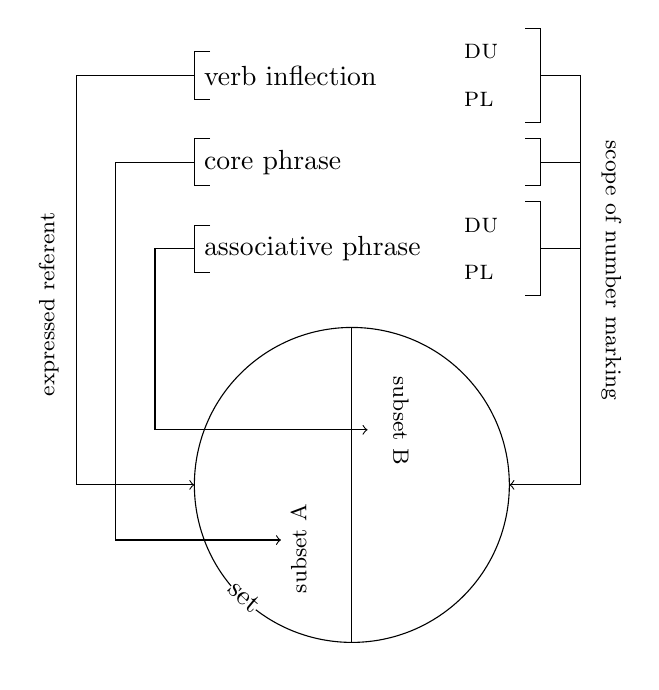
\begin{tikzpicture}
		%\path [draw=none,fill=gray, fill opacity = 0.1] (0,0) circle (2);
		\path [draw=none,fill=white, fill opacity = 1] (0,0) circle (1);
		\node [right] at (-2,5.2) {verb inflection};
		\node [right] at (1.3,5.5) {\Du};
		\node [right] at (1.3,4.9) {\Pl};
		\node [right] at (-2,3) {associative phrase};
		\node [right] at (-2,4.1) {core phrase};
		\node [right] at (1.3,3.3) {\Du};
		\node [right] at (1.3,2.7) {\Pl};
		\node [right] at (1.3,4.1) {\Nsg};
	    \draw [black,rotate=220,postaction={decorate,decoration={raise=-1ex, text effects along path, text={set}, text effects/.cd, text along path,
every character/.style={fill=white, yshift=.5ex}}}] (0,0) circle (2);
	    \draw (0,2) --(0,-2);
	    \draw (-1.8,5.5) --(-2,5.5) --(-2,4.9) --(-1.8,4.9);
		\draw (2.2,5.8) --(2.4,5.8) --(2.4,4.6) --(2.2,4.6);
		\draw (-1.8,4.4) --(-2,4.4) --(-2,3.8) --(-1.8,3.8);
		\draw (-1.8,3.3) --(-2,3.3) --(-2,2.7) --(-1.8,2.7);
		\draw (2.2,4.4) --(2.4,4.4) --(2.4,3.8) --(2.2,3.8);
		\draw (2.2,3.6) --(2.4,3.6) --(2.4,2.4) --(2.2,2.4);
		\draw [->] (-2,4.1) --(-3,4.1) --(-3,-0.7) --(-0.9,-0.7);
		\draw [->] (-2,3) --(-2.5,3) --(-2.5,0.7) --(0.2,0.7);
		\draw [->] (2.4,4.1) --(2.9,4.1) --(2.9,0) --(2,0);
		\draw (2.4,3) --(2.9,3);
		\draw (2.4,5.2) --(2.9,5.2) --(2.9,4.1);
		\draw [->] (-2,5.2) --(-3.5,5.2) --(-3.5,0) --(-2,0);
		\node[label={[label distance=0.5cm,text depth=-1ex,rotate=-90]right:\footnotesize{scope of number marking}}] at (3.2,5) {};
		\node[label={[label distance=0.5cm,text depth=-1ex,rotate=90]right:\footnotesize{expressed referent}}] at (-4,0.5) {};
		\node[label={[label distance=0.5cm,text depth=-1ex,rotate=-90]right:\footnotesize{subset B}}] at (0.5,2) {};
		\node[label={[label distance=0.5cm,text depth=-1ex,rotate=90]right:\footnotesize{subset A}}] at (-0.8,-2) {};
	\end{tikzpicture}
\caption{The inclusory construction}
\label{incluscons}
\end{figure}%\isi{inclusory} construction

\figref{incluscons} shows that the \isi{number} values differ. The core phrase is always in \isi{non-singular}. This is the expected behaviour of \isi{number} marking on \isi{nominal}s (\S\ref{formfunccase}), which makes a distinction between \isi{singular} and \isi{non-singular} leaving the subdivision between \isi{dual} and \isi{plural} to the verb inflection. As for the \isi{associative} phrase, \isi{number} marking is more specific showing agreement with the verb inflection, thus encoding \isi{dual} versus \isi{plural} instead of \isi{singular} versus \isi{non-singular}. Because the set in the \isi{inclusory} construction is minimally two, a \isi{singular} on the core phrase or a \isi{singular} in the verb inflection would be ungrammatical. For the \isi{associative} \isi{case}, there is not \isi{singular} \isi{number} value available. The enclitics \emph{=r} and \emph{=ä} encode \isi{dual} and \isi{plural} respectively.

\begin{table}
\caption{Associative case / pronominals}
\label{comcase-table}
	\begin{tabularx}{.8\textwidth}{XXXl}
		\lsptoprule
		& {person} & {dual} & {plural} \\\midrule
		\multirow{3}{3cm}{personal pronouns} &1 &\emph{ninrr} &\emph{ninä}\\
		&2 &\emph{bnrr} &\emph{bnä}\\
		&3 &\emph{nafrr} &\emph{nafä}\\
		\Recog&&\emph{bafrr}&\emph{bafä}\\
		\Indf&&\emph{nä bunrr}&\emph{nä bunä}\\
		interrogative&&\emph{mafrr}&\emph{mafä}\\
		case enclitic&&\emph{=r}&\emph{=ä}\\
		\lspbottomrule
	\end{tabularx}
\end{table}%Associative case / pronominals

The corresponding \isi{pronominal} forms of the \isi{associative} \isi{case} are shown in \tabref{comcase-table}.\footnote{I repeat here \tabref{comcase-table-1} in \S\ref{comcase}.} The relevant pronominals are personal pronouns, the \isi{recognitional} \isi{demonstrative}, the \isi{indefinite} \isi{pronoun} and the \isi{interrogative}. Two observations can be made from \tabref{comcase-table}. First, all forms include a /rr/ element for \isi{dual} and an /ä/ element for \isi{plural}. Secondly, most forms are built from the \isi{ergative} \isi{pronominal}. For example, the third \isi{person} absolutive is \emph{fi}, whereas the third \isi{person} \isi{ergative} is \emph{naf} (\Sg) or \emph{nafa} (\Nsg). The \isi{associative} third \isi{person} forms, \emph{nafrr} (\Du) and \emph{nafä} (\Pl) are formally closer to the \isi{ergative} than to the absolutive. Another example is the \isi{interrogative}, where the absolutive is \emph{mane} `who, which' and the \isi{ergative} is \emph{maf} (\Sg) and \emph{mafa} (\Nsg). The two exceptions are the first \isi{person} and the \isi{indefinite} \isi{pronoun}. The first \isi{person} \isi{non-singular} is \emph{ni}, and it neutralises the distinction between absolutive and \isi{ergative}. The \isi{indefinite} \isi{pronoun} is \emph{nä bun}, and it takes regular \isi{case} enclitics just like nouns. Therefore, \emph{nä bun} is analysed as being zero-marked, thus, absolutive.

Figure \ref{incluscons} shows that the core phrase always encodes \isi{non-singular} \isi{number}. As we have seen, this holds true for cases where there are only two participants and consequently the two subsets in the core phrase and the \isi{associative} phrase refer to a single individual respectively. The examples below show this for an ergative-marked argument, \emph{amayé nanyr} `mother with big sister' (\ref{ex605}), an absolutive-marked argument, \emph{emothé bnrr} `girl with you' (\ref{ex727}), and a dative-marked argument, \emph{sraknm nafrr} `boy with him' (\ref{ex728}). In contrasting examples without the \isi{inclusory} construction, all of these would receive a \isi{singular} marker of the respective cases. Note that the \isi{non-singular} \isi{absolutive} \emph{=é} in (\ref{ex727}) is the same as the \isi{non-singular} \isi{ergative} \emph{=é} in (\ref{ex605}). This syncretism is also found in the personal pronouns where \emph{ni} is both first \isi{person} \isi{non-singular} \isi{absolutive} and \isi{ergative} ({\S}\ref{personalpronouns-sec}). The \isi{absolutive} \isi{singular} is always zero-marked, and the \isi{non-singular} formative \emph{=é} is optional ({\S}\ref{abscase}). In the \isi{inclusory} construction, however, \isi{non-singular} \isi{number} is obligatorily encoded on the core phrase.

\begin{exe}
	\ex \emph{mni ŋagarnth amayé nanyr.}\\
	\gll mni ŋa\stem{gar}nth ama=é nane=r\\
	firewood \Stdu:\Sbj:\Nonpast:\Ipfv/break mother=\Erg.{\Nsg} {elder.sibling}=\Assoc.\Du\\
	\trans `Mother together with big sister split firewood.' (lit. `Mother with big sister, they split firewood.')\Corpus{tci20150919-05}{LNA \#140}
	\label{ex605}
\end{exe}
\begin{exe}
	\ex \emph{kabef emothé emarn bnrr.}\\
	\gll kabe=f emoth=é e\stem{mar}n bnrr\\
	man=\Erg.{\Sg} girl=\Abs.{\Nsg} \Stsg:\Sbj>\Stdu:\Obj:\Nonpast:\Ipfv/see \Second.\Du.\Assoc\\
	\trans `The man sees the girl together with you.' (lit. `The man sees them, the girl with you.')
	\label{ex727}
\end{exe}
\begin{exe}
	\ex \emph{ŋafyf sraknm dunzi ärin nafrr.}\\
	\gll ŋafe=f srak=nm dunzi ä\stem{ri}n nafrr\\
	father=\Erg.{\Sg} boy=\Dat.{\Nsg} arrow \Stsg:\Sbj>\Stdu:\Io:\Nonpast:\Ipfv/give \Third.\Du.\Assoc\\
	\trans `The father gives the arrow to the boy together with him.' (lit. `Father gives them the arrow, the boy with him.')
	\label{ex728}
\end{exe}

If the total set indexed in the verb is two, then it follows that the two phrases can only refer to a single individual, even though the core phrase has to be marked for \isi{non-singular}, as in (\ref{ex725}) and (\ref{ex605}\textendash\ref{ex728}). If the total set indexed in the verb is \isi{plural}, it is unclear whether both subsets are bigger than one or whether one of them is singular and if so, which one. Example (\ref{ex340}) above is unambiguous because the \isi{associative} phrase is expressed by a personal name (\emph{Moses}=\Assoc.\Pl). If the \isi{associative} phrase it expressed by a noun or \isi{pronoun}, we are left with contextual clues. In example (\ref{ex339}), the speaker talks about marriage customs explaining that his clan will not exchange sisters with those clans with which they share a land boundary. In this example, \emph{nafä} has to be translated as a \isi{plural} `with them'.

\begin{exe}
	\ex \emph{ni nafäwä bad wkurwre ... fi neba erä ... ni neba}\\
	\gll ni nafä=wä bad w\stem{kur}wre (.) fi neba e\stem{rä} (.) ni neba\\
	{\Fnsg} \Third\Pl.\Assoc={\Emph} ground \Fpl:\Sbj>\Tsg.\F:\Nonpast:\Ipfv/split (.) \Third.{\Abs} opposite \Stpl:\Sbj:\Nonpast:\Ipfv/be (.) \First{} opposite\\
	\trans `We really share a land boundary with them. They are there and we (are) here.' (lit. `we cut the ground with them.')\Corpus{tci20120814}{ABB \#307}
	\label{ex339}
\end{exe}

In contrast, in example (\ref{ex343}) \emph{nafä} refers to a singular `with him'. This example is taken from a text about grief, and the speaker justifies a particular mourning custom by pointing out that he and his family have shared a lifetime with the deceased person.

\begin{exe}
	\ex \emph{... bänema ni nafä kwamränzrme. ni nafä nzwamnzrm.}\\
	\gll (.) bäne=ma ni nafä kwa\stem{mrä}nzrme ni nafä nzwa\stem{m}nzrm\\
	(.) \Recog={\Char} {\Fnsg} \Third\Pl.{\Assoc} \Fpl:\Sbj:\Pst:\Dur/stroll {\Fnsg} \Third\Pl.{\Assoc} \Fpl:\Sbj:\Pst:\Dur/dwell\\
	\trans `... because we walked around with him. We lived with him.'\\\Corpus{tci20120805-01}{ABB \#830-831}
	\label{ex343}
\end{exe}

It follows that out of context the \isi{pronoun} \emph{nafä} can refer to an individual or to a group of people in (\ref{ex339}) and (\ref{ex343}). This is also true for the \isi{pronoun} \emph{ni} (\Fnsg) in both examples. I pointed out above that the core phrase is always \isi{non-singular}, even if the subset expressed by the core phrase is \isi{singular}. Hence, the \isi{pronoun} \emph{ni} can refer to an individual or a group of people, and out of context example (\ref{ex339}) can be translated as `I share land with them', `We share land with him' or `We share land with them'. What it cannot mean is `I share land with him'. For this meaning, the verb would have to index a \isi{dual} and the \isi{associative} phrase would have to be marked for \isi{dual} \isi{number}.\footnote{The inclusory construction can be seen as a syntactic equivalent to distributed exponence in the verb morphology ({\S}\ref{verbprelim}).}

In the following discussion, I want to address the question whether or not the \isi{associative} phrase and the core phrase form a constituent. From a semantic perspective, we can answer this question in the affirmative, but we can also find some structural evidence that the \isi{associative} phrase and the core phrase form a functional unit. I have shown above that the \isi{associative} phrase agrees with the verb in \isi{number}. The core phrase, on the other hand, agrees with the verb in \isi{person} and \isi{number}. The \isi{number} category is very telling because it is always \isi{non-singular}. Additionally, the core phrase is assigned the appropriate \isi{case} marker by the argument structure of the \isi{verb}. I take these points as structural evidence that the \isi{associative} phrase and the core phrase form a functional unit. However, they do not constitute a phrase. In other words, the \isi{associative} case in the \isi{inclusory} construction does not function in the way that adnominal case does. For example, the characteristic case signals that one \isi{noun phrase} is embedded into a matrix \isi{noun phrase}. There is a fixed structure for embedding, and scrambling of elements which belong to the matrix phrase is not possible in Komnzo ({\S}\ref{npstructure}). There may be several instantiations of an argument in a clause, but these \isi{noun phrase}s are always marked for the same case. As we have seen above, the \isi{associative} phrase can be moved independently of the core phrase. Moreover, most corpus examples lack a core phrase altogether. In conclusion, the \isi{inclusory} construction is different from adnominal \isi{case}, like the \isi{characteristic} or \isi{possessive} case. The core phrase and the \isi{associative} phrase are not integrated into a matrix phrase.

The \isi{inclusory} construction also differs from coordinative constructions ({\S}\ref{clausecoordination}). Example (\ref{ex726}) shows the same state-of-affairs as expressed in (\ref{ex725}) above, but using a conjunctive \isi{coordination}. The main structural differences are that in \isi{coordination}: (i) a \isi{conjunction} like \emph{a} `and' is required, (ii) the coordinated \isi{noun phrase}s have to precede and follow the \isi{conjunction}, (iii) both \isi{noun phrase}s receive the same \isi{case} marker, (iv) the \isi{case} marker can be \isi{singular}. Note that in (\ref{ex725}) above the \isi{associative} phrase \emph{Kowir} could occur in all other positions. Nevertheless, the most natural positions are either after the verb or right after \emph{Maureené}.

\begin{exe}
	\ex \emph{Maureenf a Kowif bi ynäbünth.}\\
	\gll Maureen=f a Kowi=f bi y\stem{näbü}nth\\
	maureen=\Erg.{\Sg} and kowi=\Erg.{\Sg} sago(\Abs) \Stdu:\Sbj>\Tsg.\Masc:\Obj:\Nonpast:\Ipfv/beat\\
	\trans `Maureen and Kowi beat sago.'
	\label{ex726}
\end{exe}

Furthermore, the elements in an \isi{inclusory} construction can be coordinated, as in example (\ref{ex342}), where the two \isi{associative} phrases \emph{nä oromanr} `with another old man' and \emph{nä kabe} `with another man' are part of a disjunctive \isi{coordination} connected by \emph{o} `or'.

\begin{exe}
	\ex \emph{nä oromanr o nä kaber fi bämrn.}\\
	\gll nä {oroman=r} o nä kabe=r fi b=ä\stem{m}rn\\
	{\Indf} {old.man=\Assoc.\Du} or {\Indf} man=\Assoc.{\Du} \Third.{\Abs} \Med=\Stdu:\Sbj:\Nonpast:\Ipfv/sit\\
	\trans `He is sitting there with another old man or another man.' (lit. `...with some old man or with some man they two sit there.')\Corpus{tci20111004}{RMA \#343}
	\label{ex342}
\end{exe}

There is no clear semantic difference between \isi{coordination} and the \isi{inclusory} construction, but the difference seems to be pragmatic. While \isi{coordination} places the two elements on the same rank, the \isi{inclusory} construction may be used to highlight the referent expressed in the \isi{associative} phrase. This is supported by the fact that in most corpus examples, the core phrase is omitted, because its reference has been established earlier. Example (\ref{ex342}) above was uttered as the description of a set of pictures cards. I reproduce the example in a longer context in (\ref{ex743}). The speaker talks about the protagonist of the story who is drinking with his friends. While describing the picture card, the speaker points out that the protagonist is sitting with another man. He then asks about the topic of their conversation. This other man is expressed in the \isi{associative} phrase. The same state of affairs could be expressed by a coordinative construction (`He and another man are sitting there'). The point is that the \isi{inclusory} construction can be used to introduce a new \isi{participant}, and thus has a pragmatic function. Note that the \isi{associative} phrase occurs in the first position of the clause.

\begin{exe}
	\ex \emph{ane fof yamnzr byé. wri kabenzo ... ane bramöwä ... fof ausi fäth nä berä ... ttrikasi ŋatrikwrth ... nä oromanr o nä kaber fi bämrn ... skiski warfo. monme fi yatrikwr ... nafan?}\\
	\gll ane fof ya\stem{m}nzr b=\stem{yé} wri kabe=nzo (.) ane bramöwä (.) fof ausi fäth nä b=e\stem{rä} (.) t-trik-si ŋa\stem{trik}wrth (.) nä {oroman=r} o nä kabe=r fi b=ä\stem{m}rn (.) skiski warfo monme fi ya\stem{trik}wr (.) nafan\\
	{\Dem} {\Emph} \Tsg.\Masc:\Sbj:\Nonpast:\Ipfv/sit \Med=\Tsg.\Masc:\Sbj:\Nonpast:\Ipfv/be drunk man={\Only} (.) {\Dem} all (.) {\Emph} old.woman \Dim{} {\Indf} \Med=\Stpl:\Sbj:\Nonpast:\Ipfv/be (.) \Redup-tell-{\Nmlz} \Stpl:\Sbj:\Nonpast:\Ipfv/tell (.) {\Indf} {old.man=\Assoc.\Du} or {\Indf} man=\Assoc.{\Du} \Third.{\Abs} \Med=\Stdu:\Sbj:\Nonpast:\Ipfv/sit (.) platform on.top how but \Stsg:\Sbj>\Tsg.\Masc:\Io:\Nonpast:\Ipfv/tell (.) \Tsg.\Dat\\
	\trans `That is the one sitting there. (They are) drunkards ... all of them. There is some woman. They are telling stories. He is sitting there with another old man or another man ... on the platform. But what is he telling him?'\\\Corpus{tci20111004}{RMA\#340-345}
	\label{ex743}
\end{exe}

Lichtenberk suggests two parameters for a typology of \isi{inclusory} pronominals: ``(i) do the \isi{inclusory} \isi{pronominal} and the included NP together form a syntactic construction, a phrase, or not?; and (ii) is there or is there not an overt marker of the relation between the \isi{inclusory} \isi{pronominal} and the included NP?'' (\citeyear[3]{Lichtenberk:2000hr}). This sets up a fourfold possibility space.\footnote{The four possibilities are: 1. +syntactic construction +overt marker, 2. +syntactic construction -overt marker, 3. -syntactic construction +overt marker, 4. -syntactic construction -overt marker.} The second parameter is clear for Komnzo: the \isi{associative} \isi{case} is an overt marker of the \isi{inclusory} construction. With respect to the first parameter, I hope to have shown above that Komnzo does not give a neat answer to these questions. In terms of agreement, we may say that the two elements agree, but they agree in their own ways. In terms of \isi{noun phrase} syntax, it would be a rather aberrant \isi{noun phrase}. Therefore, I suggest that Lichtenberk's typology should be expanded. A more fine-grained reformulation of his first parameter could help capture what constitutes a `syntactic construction', for example verb agreement and phrase structure. Singer's typology (\citeyear{Singer:inclu}) concentrates of the locus of where the total set is encoded. She draws a distinction between Type 1, in which the set of total participants is represented by an independent \isi{pronoun}, and Type 2, in which it is represented by a verbal affix. Komnzo clearly belongs into the Type 2 category. But we can make a case that Komnzo also belongs into Type 1 because the \isi{associative} phrase, which can be a \isi{pronoun}, encodes the number of the total set.

Lichtenberk argues that the marker of \isi{inclusory} constructions is often historically related to the coordinate \isi{conjunction} or to the \isi{comitative} case, but he adds that the \isi{inclusory} construction differs from both.\footnote{``In explicit inclusory constructions, the marker of the relation between the inclusory pronominal and the included NP is typically etymologically related either to the coordinate conjunction `and' or to the comitative marker in the language.'' (\citealt[4]{Lichtenberk:2000hr}) and ``The phrasal inclusory construction is neither coordinating nor comitative; it is a construction \emph{sui generis}.'' (\citeyear[30, emphasis in original]{Lichtenberk:2000hr})} We have seen in \S\ref{comcase} that there is no \isi{inclusory} construction and no \isi{number} distinction with inanimates, and only \emph{=ä} is attached as a case marker. With inanimates, \emph{=ä} can be analysed as \isi{comitative} \isi{case}. On the other hand, the function of \emph{=r} (\Du) and \emph{=ä} (\Pl) with animates is an \isi{inclusory} function, which differs markedly from the \isi{associative} with inanimates. I follow Lichtenberk by analysing \emph{=r} and \emph{=ä} as markers of a distinct \isi{inclusory} construction, but for practical purposes I retain the label {\Assoc} in the \isi{gloss} instead introducing a separate label for the \isi{inclusory} category.
	%!TEX root = ../main.tex

\chapter{Clausal syntax} \label{cha:clausalsyntax}

\section{Introduction}

This chapter addresses the syntax within simple clauses. In Komnzo, a large part of the argument structure is encoded in the \isi{verb} morphology. This is described in {\S}\ref{alignmtemplates}, and summarised in \tabref{argalignverbs}. Therefore, the following description of \isi{clause} types is brief for those types which have been addressed before, but more detailed for other types where the \isi{verb} morphology plays a smaller role.

\section{Constituent order}\label{constitorder}

The dominant word order in Komnzo is AUV (actor \isi{undergoer} verb). Recipients of ditransitives also precede the verb and follow the actor noun phrase, but there is no clear position with respect to the \isi{theme} argument. Evidence for basic word order comes from the use of the \isi{recognitional} \isi{demonstrative} ({\S}\ref{recognitional-pronoun-subsec}). In example (\ref{ex686}), the \isi{object} argument is expressed first by the \isi{recognitional} \emph{bäne} `those' and then by the noun \emph{züm} `centipedes'. The speaker uses the \isi{recognitional} in absolutive case in the position where the constituent normally occurs. This is a tip-of-the-tongue situation, and therefore the speaker fills in the appropriate referent after the verb. Note that there is usually a break in the intonation contour if any constituent occurs after the verb.

\begin{exe}
	\ex \emph{nzürna ŋaref \textbf{bäne} sasryoftha \textbf{züm}.}\\
	\gll nzürna ŋare=f bäne sa\stem{sryofth}a züm\\
	nzürna woman=\Erg.{\Sg} \Recog.{\Abs} \Sg:\Sbj>\Tsg.\Masc:\Io:\Pst:\Pfv/send centipede\\
	\trans `The \emph{nzürna} woman sent those ones after him ... the centipedes.'\\\Corpus{tci20120827-03}{KUT \#138}
	\label{ex686}
\end{exe}

Experiencer-object constructions ({\S}\ref{expobjconstr}) deviate from the basic word order. The \isi{experiencer} is placed almost always before the \isi{stimulus}, i.e. the \isi{undergoer} comes first and the actor follows (\ref{ex687}). This can be explained by the relative salience of the \isi{experiencer} in such constructions and the fact that it almost always ranks higher in terms of animacy.

\begin{exe}
	\ex \emph{ŋatha kawakawaf bthefaf.}\\
	\gll ŋatha kawakawa=f b=the\stem{faf}\\
	dog madness={\Erg} \Med=\Stsg:\Sbj>\Stpl:\Obj:\Rpst:\Pfv/hold\\
	\trans `The dogs went crazy there.' (lit. `Madness has grabbed the dogs.')\\\Corpus{tci20130907-02}{JAA \#488}
	\label{ex687}
\end{exe}

AUV word order is only a tendency in Komnzo. In fact, most clauses lack overt \isi{noun phrase}s for the respective constituents. The flagging of \isi{noun phrase}s with \isi{case} allows for some flexibility in the arrangement of constituents. However, deviations from the basic word order are often pragmatically motivated. In example (\ref{ex716})\footnote{Note that the stem \emph{fath-} means `hold', but in a suppressed-object construction it means `marry' ({\S}\ref{suppressedobjectclause}).}, the speaker replies to a question whether a particular individual is his brother in-law. He says `really my brother in-law' and then gives an explanation in the following clause, where the \isi{undergoer} appears before the actor. The reversal of constituents can be explained as a strategy to focus the \isi{undergoer} argument, that is \emph{mayawa emoth} `Mayawa sister' is focussed by fronting.

\begin{exe}
	\ex \emph{nzone ngom fof ... \textbf{mayawa emoth} naf zefafa fof.}\\
	\gll nzone ngom fof (.) mayawa emoth naf ze\stem{faf}a fof\\
	\Fsg.{\Poss} brother.in.law {\Emph} (.) mayawa girl \Tsg.{\Erg} \Sg:\Sbj:\Pst:\Pfv/marry \Emph\\
	\trans `My brother in-law ... He married a Mayawa sister.'\Corpus{tci20120814}{ABB \#391-392}
	\label{ex716}
\end{exe}

In example (\ref{ex688}), both constituents follow the verb. The \isi{undergoer} comes first and after a short pause the actor follows. Examples like these are rare, but frequently one of the constituents follows the verb. This can occur because the speaker wants to clarify the state of affairs or because she wants to put emphasis on the referent. There is usually a break in the intonation contour after the verb form.

\begin{exe}
	\ex \emph{keke thufnzrm ane karma kabe ... naf.}\\
	\gll keke thu\stem{fn}nzrm ane kar=ma kabe (.) naf\\
	{\Neg} \Sg:\Sbj>\Stpl:\Obj:\Pst:\Dur/kill {\Dem} village={\Char} man (.) \Tsg.\Erg\\
	\trans `She did not attack those village people.'\Corpus{tci20120901-01}{MAK \#50}
	\label{ex688}
\end{exe}

While the order of constituents is flexible to some extent, it is rarely the case that other elements follow the verb, like adverbs, TAM particles, or the \isi{negator}. Komnzo supports a number of cross-linguistic generalisations found in verb final languages (\citealt{Dryer:2007wordorder}), for example that the \isi{possessor} precedes the \isi{possessed}. A second generalisation is that verb-final languages tend to have postpositions rather than prepositions. Komnzo does not have a category of adpositions, but \isi{locational} nouns like \emph{tharthar} `side' or \emph{mrmr} `inside' always follow the noun whose location they specify ({\S}\ref{locationals-sec}).

\section{Clause types}\label{clause types}

\subsection{Non-verbal clauses}\label{nonverbalclauses}

Non-verbal clauses are a marginal phenomenon in Komnzo. This section describes the few types of verbless clauses. These are usually short one or two word utterances including an element which has some verb-like semantics, for example TAM particles or property nouns.

The TAM particles \emph{kwa} {\Fut} and \emph{kma} {\Pot} can stand alone when they are used as commands. For example, \emph{kma} can mean `You have to!', and with the \isi{apprehensive} clitic \emph{=m} attached, it can mean the opposite: \emph{kmam} `You must not!'. In example (\ref{ex560}), the \isi{future} particle \emph{kwa} is used in the sense of `Wait!'. The speaker describes poison-root fishing and how they have to hold back the children from jumping into the water too early.

\begin{exe}
 	\ex \emph{katakatan kwa zöbthé thrängathinzth nima ``\textbf{kwa}! komnzo \textbf{kwa}!''}\\
 	\gll kata-katan kwa zöbthé thrän\stem{gathinz}th nima kwa komnzo kwa\\
	\Redup-small {\Fut} first \Stpl:\Sbj>\Stpl:\Obj:\Irr:\Pfv:\Venit/stop {\Quot} wait only wait\\
 	\trans `First, they will hold back the small ones and say: ``Wait! Just Wait!'''\\\Corpus{tci20110813-09}{DAK \#25}
 	\label{ex560}
\end{exe}

Another possible type of verbless \isi{clause} is with the property nouns \emph{miyo} `desire' and \emph{miyatha} `knowledge' and their antonyms \emph{miyomär} `aversion, dislike' and \emph{miyamr} `ignorance'. These words are usually used as \isi{nominal} predicates with light verbs or with the \isi{copula}. As a consequence, we find examples like ({\ref{ex561}}), where the last \isi{clause} \emph{nzä miyamr} does not contain a verb. It is possible to insert the \isi{copula} in the appropriate inflection (\emph{worera} \Fsg:\Sbj:\Pst:\Ipfv/be), but often it is left out. Apart from examples like these, there are no verbless clauses in Komnzo.

\begin{exe}
	\ex \emph{fi kafar mane erera näbi ane ofe ŋarerath. mobo erera? ... \textbf{nzä miyamr}}\\
	\gll fi kafar mane e\stem{rä}ra näbi ane ofe ŋa\stem{rä}rath. mobo e\stem{rä}ra (.) nzä miyamr\\
	but big which \Stpl:\Sbj:\Pst:\Ipfv/be one {\Dem} disappearance \Stpl:\Sbj:\Pst:\Ipfv/do where.{\All} (.)  \Stpl:\Sbj:\Pst:\Ipfv/be \Fsg.{\Abs} ignorance\\
	\trans `As for the big dogs, they disappeared for good. Where did they go? ... I (do) not know.'\Corpus{tci20111119-03}{ABB \#70-72}
	\label{ex561}
\end{exe}

\subsection{Copula clauses}\label{copclause}

Copula clauses are a subtype of \isi{non-verbal} \isi{predication}. They are described here in a separate subsection because the \isi{copula} shows a number of idiosyncrasies. First, the \isi{copula} has no \isi{restricted stem}. Note that this can be predicted because the main function of the \isi{restricted stem} is to express the \isi{perfective} \isi{aspect}. Secondly, the stem of the \isi{copula} is sensitive to duality: the non-dual stem is \emph{rä}, while the dual stem is \emph{rn}. Thirdly, the third \isi{person} singular inflections are irregular (in the non-past): \isi{masculine} \emph{yé}; \isi{feminine} \emph{rä}. \tabref{copulanonpast} shows the \isi{copula} forms in \isi{non-past}, \isi{recent past} and \isi{past} \isi{tense}. Finally, the \isi{copula} stem \emph{rä} can be used in an ambifixing template with the meaning `do'. This last point is discussed as part of the description of light verbs in \S\ref{lightverb}.

\begin{table}[H]
\caption{Copula inflection}
\label{copulanonpast}
	\begin{tabularx}{\textwidth}{XXXXXl}
		\lsptoprule
		&\Nonpast&\Rpst &\Rpst:\Dur& \Pst&\Pst:\Dur\\\midrule
		\Fsg&\emph{worä}&\emph{kwofrä}&\emph{worärm}&\emph{worera}&\emph{kwofräm}\\
		\Fdu&\emph{nrn}&\emph{nzfrn}&\emph{nrnm}&\emph{nrna}&\emph{nzfrm}\\
		\Fpl&\emph{nrä}&\emph{nzfrä}&\emph{nrärm}&\emph{nrera}&\emph{nzfrärm}\\
		\Ssg&\emph{nrä}&\emph{nzfrä}&\emph{nrärm}&\emph{nrera}&\emph{nzfrärm}\\
		\Tsg.\F&\emph{rä}&\emph{zfrä}&\emph{rärm}&\emph{rera}&\emph{zfrärm}\\
		\Tsg.\Masc&\emph{yé}&\emph{sfrä}&\emph{yrärm}&\emph{yara}&\emph{sfrärm}\\
		\Stdu&\emph{ern}&\emph{thfrn}&\emph{ernm}&\emph{erna}&\emph{thfrnm}\\
		\Stpl&\emph{erä}&\emph{thfrä}&\emph{erärm}&\emph{erera}&\emph{thfrärm}\\
		\lspbottomrule
	\end{tabularx}
\end{table}%Copula inflection

The \isi{copula} takes a \isi{copula} \isi{subject} and a \isi{copula} \isi{complement}. Copula clauses may express identity between two NPs (\ref{ex611}). They are used in presentational constructions; usually with a \isi{clitic} \isi{demonstrative} (\ref{ex612}).

\begin{exe}
	\ex \emph{ni fthé miyatha zäkorake ``babai zane bthan kabe yé.''}\\
	\gll ni fthé miyatha zä\stem{kor}ake babai zane bthan kabe \stem{yé}\\
	{\Fnsg} when knowledge \Fpl:\Sbj:\Pst:\Pfv/become uncle \Dem:{\Prox} black.magic man \Tsg.\Masc:\Sbj:\Nonpast:\Ipfv:\Cop\\
	\trans `That was when we realised ``The uncle is this sorcerer.'''\Corpus{tci20130901-04}{RNA \#45}
	\label{ex611}
\end{exe}
\begin{exe}
	\ex \emph{yorär ziyé ... zikogr.}\\
	\gll yorär z=\stem{yé} (.) z=y\stem{kogr}\\
	yorär \Prox=\Tsg.\Masc:\Sbj:\Nonpast:\Ipfv/be (.) \Prox=\Tsg.\Masc:\Sbj:\Nonpast:\Stat/stand\\
	\trans `Yorär (Syzygium sp) is here. It stands here.'\Corpus{tci20130907-02}{JAA \#450-451}
	\label{ex612}
\end{exe}

The \isi{complement} may be marked with the \isi{proprietive} case (\S\ref{propcase}) or the \isi{privative} case (\S\ref{privcase}) to express the existence or non-existence of some entity in relation to the \isi{copula} \isi{subject}. The former is shown in (\ref{ex744}), where they speaker literally says `the village is with a name' to express that it has some reputation. The latter is shown in (\ref{ex745}), where the speaker tells how he was looking for a creek that carried water.

\begin{exe}
	\ex \emph{zane kar mane rä yfkarä rä.}\\
	\gll zane kar mane \stem{rä} yf=karä \stem{rä}\\
	\Dem:{\Prox} village which \Tsg.\F:\Sbj:\Nonpast:\Ipfv:\Cop{} name={\Prop} \Tsg.\F:\Sbj:\Nonpast:\Ipfv:\Cop{}\\
	\trans `As for this village, it has a (good) reputation.'\Corpus{tci20120805-01}{ABB 447-448}
	\label{ex744}
\end{exe}
\begin{exe}
	\ex \emph{buyak we ttfö ane zräbrmé nimame ... keke ... nomär rä.}\\
	\gll b=wi\stem{yak} we ttfö ane zrä\stem{brm}é nima=me (.) keke (.) no=mär \stem{rä}\\
	\Med=\Fsg:\Sbj:\Nonpast:\Ipfv/walk also creek {\Dem} \Fsg:\Sbj:\Irr:\Pfv/follow like.this={\Ins} (.) {\Neg} (.) water={\Priv} \Tsg.\F:\Sbj:\Nonpast:\Ipfv:\Cop\\
	\trans `I walked there, I followed another creek like this ... No ... (The creek) had no water.'\Corpus{tci20130903-03}{MKW \#92-93}
	\label{ex745}
\end{exe}

Adjectives and property nouns may also be \isi{copula} complements, as shown in (\ref{ex746}) and (\ref{ex747}), respectively. In (\ref{ex746}), the speaker reports how his fathers were comparing their yam harvest. In example (\ref{ex747}), the speaker talks about how as a teenager she was afraid of the anthropologist Mary Ayres when she first visited Rouku.

\begin{exe}
	\ex \emph{katakatanwä thfrä! nzenme kafar erä!}\\
	\gll kata-katan=wä thf\stem{rä} nzenme kafar e\stem{rä}\\
	\Redup-small={\Emph} \Tpl:\Sbj:\Rpst:\Ipfv:\Cop{} \Fnsg:{\Poss} big \Tpl:\Sbj:\Nonpast:\Ipfv:\Cop\\
	\trans `Their (yams) were a bit small! Our (yams) are big!'\Corpus{tci20120805-01}{ABB 403}
	\label{ex746}
\end{exe}
\begin{exe}
	\ex \emph{nzä wwtri kwarärm ... markaianema ... nafanema fof.}\\
	\gll nzä w-wtri kwa\stem{rä}rm (.) markai=ane=ma (.) nafane=ma fof\\
	\Fsg.{\Abs} \Redup-fear \Fsg:\Sbj:\Pst:\Dur:\Cop{} (.) outsider=\Poss.\Sg={\Char} (.) \Tsg.\Poss={\Char} \Emph\\
	\trans `I was a bit afraid ... of the white woman ... really (afraid) of her.'\\\Corpus{tci20130911-03}{MBR \#10-11}
	\label{ex747}
\end{exe}

\subsection{Intransitive clauses}\label{intransitiveclauses}

In terms of \isi{verb} morphology, \isi{intransitive} clauses have been described in {\S}\ref{morphologicaltemplates}. The verb inflection employs the prefixing or the \isi{middle} template. Their single argument is always in \isi{absolutive} \isi{case}. Two examples are given in (\ref{ex562}) and (\ref{ex563}).

The two prefixing verbs in (\ref{ex562}) have no overt \isi{subject} noun phrases, but the second \isi{clause} contains an adjunct marked with the \isi{purposive} \isi{case} \emph{karr} `for a village' (or settlement place). In example (\ref{ex563}), we see the \isi{middle} verb \emph{brigsi} `return' and the \isi{subject} \isi{pronoun} \emph{nzä} in absolutive \isi{case}.

\begin{exe}
	\ex \emph{ŋarsenzo \textbf{swanyakm} ... karr \textbf{swanrenzrm}.}\\
	\gll ŋars=en=nzo swan\stem{yak}m (.) kar=r swan\stem{re}nzrm\\
	river=\Loc={\Only} \Tsg.\Masc:\Sbj:\Pst:\Dur:\Venit/walk (.) village={\Purp} \Tsg.\Masc:\Sbj:\Pst:\Dur:\Venit/look.around\\
	\trans `He was coming along the river ... he was looking for a place to settle.'\\\Corpus{tci20120922-09}{DAK \#14-15}
	\label{ex562}
\end{exe}
\begin{exe}
	\ex \emph{nzä boba fthé kanathrfa \textbf{zänbrima}.}\\
	\gll nzä boba fthé kanathr=fa zän\stem{brim}a\\
	\Fsg.{\Abs} \Med.{\Abl} when kanathr={\Abl} \Sg:\Sbj:\Pst:\Pfv:\Venit/return\\
	\trans `That was when I returned from Kanathr.'\Corpus{tci20120805-01}{ABB \#607}
	\label{ex563}
\end{exe}

\subsection{Impersonal clauses}\label{impersonalclause}

Impersonal clauses are expressed using the \isi{middle} template of the verb, in which a person-invariant \isi{middle} marker fills the prefix slot, while the suffix indexes the single argument of the predicate ({\S}\ref{middletemplatesubsection}). The indexed noun phrase, if present at all, occurs in \isi{absolutive} \isi{case}. The salient feature of this \isi{clause} type is that the referent of the verb indexing is \isi{impersonal}, unclear or simply empty. Consider examples (\ref{ex737}) and (\ref{ex738}). In the first example, the speaker talks about rain-making magic, which involves a rotting mixture of meat and honey in bottles. These bottles or containers are opened and the rising odor is said to increase the rainfall. The third singular indexed by the verb form \emph{kfäkor} refers to the changed weather conditions, and the \ili{English} translation `it was enough' exhibits the same general or \isi{impersonal} meaning. The second example contains the noun \emph{aki} `moon', but it is unclear whether the verb really indexes this noun or whether its referent is empty. Hence, the two possible translations. During the transcription of example (\ref{ex738}), the first translation was the preferred one in this particular context.

\begin{exe}
	\ex \emph{watikthénzo fthé kfäkor ... we sgu thwäthbe woz thwärmäne.}
	\gll watik-thé=nzo fthé kfä\stem{kor} (.) we sgu thwä\stem{thb}e woz thwä\stem{rmän}e\\
	enough-\Adlzr={\Only} when \Stsg:\Sbj:\Iter/become (.) also plug \Fpl:\Sbj>\Stpl:\Obj:\Iter/put.inside bottle \Fpl:\Sbj>\Stpl:\Obj:\Iter/close\\
	\trans `When it was enough, we put the lids back in and we closed the bottles.'\\\Corpus{tci20110810-01}{MAB \#59-62}
	\label{ex737}
\end{exe}
\begin{exe}
	\ex \emph{aki zbo kräkor.}\\
	\gll aki zbo krä\stem{kor}\\
	moon \Prox.{\All} \Stsg:\Sbj:\Irr:\Pfv/become\\
	\trans `It became moon(light) here.' or `The moon came up here.'\Corpus{tci20120904-02}{MAB \#47}
	\label{ex738}
\end{exe}

Example (\ref{ex557}) is a description of a picture as part of a stimulus task. The speaker takes on the role of a man in the picture and asks: `What is going on?'. Again, the verb form \emph{krewär} appears in the \isi{middle} construction and indexes a third singular.

\begin{exe}
	\ex \emph{sinzo foba ynrä nima ``ra krewär bobo?''}\\
	\gll si=nzo foba yn\stem{rä} nima ra kre\stem{wär} bobo\\
	eye={\Only} \Dist.{\Abl} \Tsg.\Masc:\Sbj:\Nonpast:\Ipfv:\Venit/be {\Quot} what(\Abs) \Stsg:\Sbj:\Irr:\Pfv/happen \Med.{\All}\\
	\trans `He was just looking from over there and wondered: ``What is going on there?'''\Corpus{tci20111004}{RMA \#353}
	\label{ex557}
\end{exe}

Impersonal constructions often involve light verbs, for example \emph{rä-} `do' and \emph{ko-} `become', which take a \isi{nominal} predicate, for example a noun or \isi{property noun}. In these cases, the \isi{nominal} predicate will be unmarked for \isi{case}, like the absolutive \isi{case}. Therefore, it may be difficult to decide whether (i) it is a \isi{nominal} predicate and the \isi{subject} is empty, or (ii) whether the noun phrase in question is the \isi{subject} indexed in the \isi{verb}. Consider example (\ref{ex559}), in which the speaker describes the location of the mythical place of origin \emph{Kwafar}, which is located in the Arafura sea between Papua New Guinea and Australia. The verb form \emph{ŋakonzr} `it becomes' occurs in the \isi{relative clause}, which is printed in boldface. The third singular indexed in the verb form could be \emph{mazo} `ocean' (lit. `where the ocean becomes') or it could be an empty \isi{subject} (lit. `it becomes ocean').

\begin{exe}
	\ex \emph{thden rera ... zane zena mane bad mane wythk \textbf{mazo mä ŋakonzr} a ... australiane bad mä wythk.}\\
	\gll thd=en \stem{rä}ra (.) zane zena mane bad mane w\stem{ythk} mazo mä ŋa\stem{ko}nzr a (.) australia=ane bad mä w\stem{ythk}\\
	middle=Loc{} \Tsg.\F:\Sbj:\Pst:\Ipfv/be (.) \Dem:{\Prox} today which ground which \Tsg.\F:\Sbj:\Nonpast:\Ipfv/come.to.end and (.) australia={\Poss} ground where \Tsg.\F:\Sbj:\Nonpast:\Ipfv/come.to.end\\
	\trans `It was in the middle ... this one, where the land ends ... where it becomes ocean until where Australia's land ends.'\Corpus{tci20131013-01}{ABB \#26-30}
	\label{ex559}
\end{exe}

Weather events often have empty or \isi{impersonal} subjects. This can be shown with prefixing verbs as well as \isi{middle} verbs. A common way to say `It is going to rain' is shown in (\ref{ex739}). It is clear that \emph{nor} `for rain' is not indexed in the verb because it is flagged with a non-core \isi{case}, the \isi{purposive} \isi{case}. Therefore, the reference of the third singular in the verb form is empty.

\begin{exe}
	\ex \emph{nor yé.}\\
	\gll no=r \stem{yé}\\
	rain={\Purp} \Tsg.\Masc:\Sbj:\Nonpast:\Ipfv/be\\
	\trans `It will rain.' (lit. `It is for rain'){\hspace*{1pt}\hfill{\footnotesize{[overheard]}}}
	\label{ex739}
\end{exe}

Another example is the phrase \emph{wär kwan yanor} `it is thundering' in (\ref{ex740}). The thunder is expressed by the \isi{ideophone} \emph{wär kwan} `thundering noise', and all ideophones of this type are \isi{nominal} compounds headed by \emph{kwan} `noise, sound' ({\S}\ref{ideophones-sec}). The verb \emph{yannor} is inflected for a masculine subject, but \emph{kwan} is feminine. Hence \emph{wär kwan} is not the \isi{subject}, and a literal translation would be: `He shouts the thunder sound'. Again the reference of `he' is empty.

\begin{exe}
	\ex \emph{wär kwan yanor.}\\
	\gll {wär kwan} ya\stem{nor}\\
	thunder \Tsg.\Masc:\Sbj:\Nonpast:\Ipfv/shout\\
	\trans `It is thundering.'{\hspace*{1pt}\hfill{\footnotesize{[overheard]}}}
	\label{ex740}
\end{exe}

Other weather or sound phenomena can be expressed by verbs in the \isi{middle} template. In example (\ref{ex558}), the verb `start' is inflected for a \Stsg{} \isi{subject}, but its referent is unclear \textendash{} partly because the verb does not index an \isi{object}. Thus, the indexed argument could be (i) the sound of the fire (`The fire sound started'), or (ii) it could be an empty \isi{subject} (`It started the fire sound').

\begin{exe}
	\ex \emph{fi mni zürnane u kwan zethkäfako.}\\
	\gll fi mni zürn=ane {u kwan} ze\stem{thkäf}ako\\
	but fire smoke=\Poss.{\Sg} {roaring.sound} \Sg:\Sbj:\Pst:\Pfv:\Andat/start\\
	\trans `but the fire smoke's sound started (rumbling).'\Corpus{tci20120827-03}{KUT \#186-187}
	\label{ex558}
\end{exe}

\subsection{`Passive' clauses}\label{passiveclause}

Passives meanings are expressed in two ways: (i) by a \isi{verb} in the \isi{middle} template which indexes a \isi{patient} role; the indexed noun phrase occurs in \isi{absolutive} \isi{case} ({\S}\ref{middletemplatesubsection}), or (ii) by a resultative construction, in which a nominalised verb is flagged with the \isi{instrumental} \isi{case} ({\S}\ref{inscase}). Note that both are not dedicated \isi{passive} constructions. Instead, they should be understood as constructions which can express passive-like semantics.

Example (\ref{ex554}) shows both constructions. The first two clauses are in a \isi{temporal} relationship to the last clause, which is signalled by \emph{fthé} `when'. This is not a subordinate relationship because \emph{fthé} can also be used in independent clauses with the meaning of `that was when'. In the first clause, the single argument of the verb is \emph{bad} `ground, earth'. This can be translated either as an \isi{reflexive}/\isi{impersonal} `the earth created (itself)' or as a \isi{passive} `the earth was created'. In the second clause, matters are clear because the verb is in a \isi{transitive} template which shows actor agreement with `father' (\Erg) and \isi{undergoer} agreement with `earth' (\Abs), thus: `the father created the earth'. The last clause is a resultative construction. The nominalised verb \emph{rifthzsi} `hiding' takes the \isi{instrumental} case (`with hiding'), which is best translated as a \isi{passive} (`was hidden').

\begin{exe}
	\ex \emph{\textbf{bad fthé ŋafiyokwa} ... ŋafyf fthé bad wäfiyokwa ... \textbf{kidn ane rifthzsime zfrärm}.}\\
	\gll bad fthé ŋa\stem{fiyok}wa (.) ŋafe=f fthé bad wä\stem{fiyok}wa (.) kidn ane rifthz-si=me zf\stem{rä}rm\\
	earth when \Sg:\Sbj:\Pst:\Ipfv/make (.) father=\Erg.{\Sg} when earth \Stsg:\Sbj>\Tsg.\F:\Obj:\Pst:\Ipfv/make (.) {eternal fire} {\Dem} hide-\Nmlz={\Ins} \Tsg.\F:\Sbj:\Pst:\Dur/be\\
	\trans `When the earth was made ... when God made the earth ... that eternal fire was hidden.'\Corpus{tci20120909-06}{KAB \#61-63}
	\label{ex554}
\end{exe}

\subsection{Reflexive and reciprocal clauses}\label{reflrecipclause}

Formally, \isi{reflexive}/\isi{reciprocal} clauses are encoded by (i) the verb form in the \isi{middle} template and (ii) the argument noun phrase in \isi{absolutive} case. Ditransitives show exceptional grammatical behaviour in that the argument may be in absolutive or \isi{ergative} \isi{case}. There is no distinction between reflexives and reciprocals other than the fact that singulars do not allow a \isi{reciprocal} reading. Below I will describe how \isi{reflexive}/reciprocals differ from \isi{intransitive} and \isi{impersonal} \isi{clause} on the one side, and from \isi{suppressed-object} constructions on the other. This topic is also addressed in the description of the \isi{middle} template ({\S}\ref{middletemplatesubsection}).

In example (\ref{ex566}) the speaker talks about a ritual which chases away evil spirits. This rather gruesome ritual involves young men shooting at each other with blunt arrows. In the last clause of the example the noun phrase \emph{kabe} `man' is in absolutive \isi{case} and the verb employs the \isi{middle} template and indexes one argument (\Stpl). The verb \emph{rusi} `shoot' has rather clear \isi{transitive} semantics and, thus, invites a \isi{reciprocal} interpretation.

\begin{exe}
	\ex \emph{kabe kwaruthrmth frkkarä.}\\
	\gll kabe kwa\stem{ru}thrmth frk=karä\\
	man(\Abs) \Stpl:\Sbj:\Pst:\Dur/shoot blood=\Prop\\
	\trans `The people were shooting at each other (until) they were bleeding.'\Corpus{tci20150906-10}{ABB \#414}
	\label{ex566}
\end{exe}

In most cases only secondary information disambiguates between \isi{intransitive}, \isi{impersonal} and \isi{reflexive}/\isi{reciprocal} interpretations. By secondary information, I mean (i) context, (ii) grammatical devices which are not used solely for \isi{reflexive}/\isi{reciprocal} constructions, (iii) statistical tendencies of individual verbs. I will address these in turn. First, context is probably the most important, and it is evident that an example like (\ref{ex566}) is usually preceded or followed by a description which disambiguates the state of affairs. Secondly, speakers may choose to repeat the absolutive noun phrase to make clear that the intended reading should be a \isi{reciprocal} one. Consider example (\ref{ex567}), which concludes a headhunting story. The \isi{pronoun} \emph{fi} occurs twice. Additionally, the utterance was accompanied by appropriate gestures to clarify the intended \isi{reciprocal} meaning. The \isi{pronoun} \emph{fi} is marked with the \isi{exclusive} \isi{enclitic} \emph{=nzo}. The repetition and the \isi{exclusive} \isi{enclitic} are secondary strategies which are not solely used to mark \isi{reflexive}/\isi{reciprocal} meanings. Note that the \isi{exclusive} \isi{enclitic} \emph{=nzo} shows cognates in other \ili{Yam languages}. In \ili{Nen}, there is a set of \isi{reflexive}/\isi{reciprocal} pronouns which all end in \emph{nzo}, for example \emph{benzo} \Ssg{} (\citealt[1072]{Evans:2015wy}). In Komnzo, the \isi{exclusive} clitic expresses the meaning of `only' without \isi{reflexive}/\isi{reciprocal} semantics.

\begin{exe}
	\ex \emph{ni woga tüfrmäre nrä ... bänema nzenme thden ane fof kwakwirm ... woga \textbf{finzo} \textbf{finzo} kwafnzrmth.}\\
	\gll ni woga tüfr=märe n\stem{rä} (.) bäne=ma nzenme thd=en ane fof kwa\stem{kwir}m (.) woga fi=nzo fi=nzo kwa\stem{fn}nzrmth\\
	{\Fnsg} man plenty={\Priv} \Fpl:\Sbj:\Nonpast:\Ipfv/be (.) \Dem:\Med={\Char} \Fnsg.{\Poss} \isi{middle}={\Loc} {\Dem} {\Emph} \Stsg:\Sbj:\Pst:\Dur/run (.) man \Third.\Abs={\Only} \Third.\Abs={\Only} \Stpl:\Sbj:\Pst:\Dur/kill\\
	\trans `We are not many ... because this was going on in our \isi{middle} ... The people, this (group) and that (group) were killing each other.'\Corpus{tci20111107-01}{MAK \#157-158}
	\label{ex567}
\end{exe}

Although stems may alternate between different morphological templates, there is a statistical tendency to occur in a particular template for a particular stem. For example, typically \isi{transitive} meanings (\emph{rusi} `shoot', \emph{zan} `hit, kill', \emph{marasi} `see') occur most of the time in the ambifixing \isi{transitive} template. If such stems occur in a \isi{middle} template, it invites a \isi{reflexive}/\isi{reciprocal} reading rather than an \isi{impersonal} or \isi{intransitive} one. We will see in the following section that the \isi{middle} template can also be used for the \isi{suppressed-object} construction ({\S}\ref{suppressedobjectclause}). However, in the \isi{suppressed-object} construction the noun phrase indexed in the verb form is marked for \isi{ergative} \isi{case} and not absolutive. On the other hand, stems which occur in the \isi{middle} template most of the time (\emph{maikasi} `wash', \emph{bringsi} `return') should be analysed as reflexiva tanta (\citealt{Geniusienie:1987refl}), even though they may occur in the ambifixing \isi{transitive} template (`wash someone', `bring back someone'). Hence, there is a statistical tendency for stems to occur in a particular template, which helps to disambiguate between an \isi{impersonal} or \isi{reflexive}/\isi{reciprocal} reading.

Next, I want to set \isi{reflexive}/reciprocals apart from what I call the \isi{suppressed-object} construction ({\S}\ref{suppressedobjectclause}). The state of affairs in \isi{reflexive}/reciprocals is such that the actor and \isi{patient} can be exchanged. In Komnzo, both are expressed by one noun phrase which occurs in absolutive case. Herein lies the formal difference to the \isi{suppressed-object} construction. If the noun phrase \emph{kabe} `people' in example (\ref{ex566}) was in \isi{ergative} \isi{case} \textendash{} for example \emph{kabe=yé} (man=\Erg.{\Nsg}) \textendash{} the sentence would mean `they were shooting (at sth.)'. This is the \isi{suppressed-object} construction, which I describe in the following section ({\S}\ref{suppressedobjectclause}). Note that the verb form \emph{kwaruthrmth} remains the same, only the \isi{case} marking changes.

For \isi{ditransitive} verbs, the \isi{case} marking is less fixed, and the argument noun phrase can appear in absolutive as well as \isi{ergative} \isi{case}, both with a \isi{reflexive}/\isi{reciprocal} meaning. In example (\ref{ex568}), the verb form \emph{ŋarinth} indexes only the \isi{subject} (\Stdu), while the prefix slot is filled with the \isi{middle} marker. The \isi{subject} argument appears in the \isi{ergative} (\emph{nafa}). A \isi{suppressed-object} reading is not possible with \isi{ditransitive} verbs. Note that the argument could also occur in absolutive \isi{case} (\emph{fi}). This would create a \isi{clause} with two absolutive noun phrases. Hence, the choice between \isi{ergative} and abolutive seems to be dependent on the kinds of referents. In (\ref{ex568}), both noun phrases are animate, and the use of the \isi{ergative} \isi{case} avoids confusion between \isi{agent} (`they') and \isi{theme} (`sisters').

\begin{exe}
 	\ex \emph{emoth nafa ŋarinth fof.}\\
 	\gll emoth nafa ŋa\stem{ri}nth fof\\
 	girl \Tnsg.{\Erg} \Stdu:\Sbj:\Nonpast:\Ipfv/give {\Emph}\\
 	\trans `They give each other sisters.'\Corpus{tci20120805-01}{ABB \#158}
 	\label{ex568}
\end{exe}

At this stage, it is impossible to investigate this topic further, because (i) \isi{noun phrase}s are frequently omitted and (ii) as I have argued in {\S}\ref{ambifixingtemp}, except for a few verbs (\emph{yarisi} `give', \emph{trikasi} `tell', \emph{fänzsi} `show') all \isi{ditransitive} verbs are derived.

\subsection{Suppressed-object clauses}\label{suppressedobjectclause}

Suppressed-\isi{object} clauses employ the \isi{middle} template of the verb. The argument indexed in the verb is treated like an actor by the case system, i.e. it is flagged with the \isi{ergative} \isi{case}. The \isi{object} may be overtly expressed with a noun phrase, but it is suppressed from indexation in the verb form.

I describe in {\S}\ref{middletemplatesubsection} that almost all \isi{transitive} verbs can enter into the \isi{suppressed-object} construction for semantic as well as pragmatic reasons. For example, most of the time, the referents of suppressed-objects rank low in the animacy hierarchy (\citealt{Silverstein:1976vo}). In example (\ref{ex569}), the speaker searches her shoes and complains that her friend has been wearing them. We only know about the \isi{object} of \emph{rgsi} `wear' from the previous context since it is not expressed as a noun phrase, nor is the \isi{object} indexed in the verb form. The semantics of \emph{rgsi} renders a \isi{reflexive} reading (`she wears herself') non-sensical. Additionally, the fact that the \isi{subject} is in \isi{ergative} case (\emph{naf}) rules out the \isi{reflexive}/\isi{reciprocal} interpretation. This is important because the verb form is identical between \isi{reflexive}/reciprocals and the \isi{suppressed-object} construction.

\begin{exe}
	\ex \emph{ebar zfthnzo! naf rar ŋargwrm?}\\
	\gll ebar zfth=nzo naf ra=r ŋa\stem{rg}wrm\\
	head base={\Only} \Tsg.{\Erg} what={\Purp} \Sg:\Sbj:\Rpst:\Dur/wear\\
	\trans `Thickhead! Why was she wearing (the flipflops)?'\Corpus{tci20130901-04}{RNA \#173}
	\label{ex569}
\end{exe}

Objects can be suppressed for pragmatic reasons, often in addition to their low rank on the animacy hierarchy. That is because the suppression of the \isi{object} has the pragmatic effect of focussing the \isi{subject}. Example (\ref{ex570}) is taken from a text about food taboos. This topic came up while talking about a very old woman, whose old age was ascribed to her respecting all food taboos. In the example, the speaker shifts the topic from the old woman to those people who did not respect food taboos. This shift of topic is achieved by (i) a fronted \isi{relative clause} and (ii) the \isi{suppressed-object} construction. As in the previous example, we only know about the \isi{object} of \emph{rirksi} `respect, avoid' from the preceding context.

\begin{exe}
	\ex \emph{fi mafa keke kwarirkwrmth ... watik tekmär esufakwa.}\\
	\gll fi mafa keke kwarirkwrmth ... watik tekmär esufakwa\\
	but who.\Nsg.{\Erg} {\Neg} \Stpl:\Sbj:\Pst:\Dur/respect (.) then duration={\Priv} \Stpl:\Sbj:\Pst:\Ipfv/grow.old\\
	\trans `But those who did not respect (the food taboos) ... well, they grew old quickly.'\Corpus{tci20120922-26}{DAK \#26-27}
	\label{ex570}
\end{exe}

Although the \isi{object} is suppressed from indexation in the verb form, it may occur as a noun phrase in the \isi{clause}. In example (\ref{ex571}), the speaker talks about garden magic and people who steal the soil from other people's gardens. In the \isi{relative clause}, the \isi{object} \emph{bad} `ground' is suppressed from indexation in the verb, yet it appears as a noun phrase. The \isi{subject} is indexed in the verb suffix and the corresponding noun phrase, the relative \isi{pronoun} \emph{mafa}, is in \isi{ergative} case.

\begin{exe}
	\ex \emph{nä kabenzo nnzä wawa gamokarä erä bad mafa ŋakarkwrth.}\\
	\gll nä kabe=nzo nnzä wawa gamo=karä e\stem{rä} bad mafa ŋa\stem{kark}wrth\\
	{\Indf} man={\Only} perhaps yam spell={\Prop} \Stpl:\Sbj:\Nonpast:\Ipfv/be ground who.\Erg.{\Nsg} \Stpl:\Sbj:\Nonpast:\Ipfv/take\\
	\trans `Perhaps only other people, who take the soil away, have yam magic.'\\\Corpus{tci20130822-08}{JAA \#42}
	\label{ex571}
\end{exe}

The \isi{suppressed-object} may also be a \isi{relative clause}, as in example (\ref{ex572}), which is taken from a picture stimulus task.

\begin{exe}
	\ex \emph{emothf ŋatrikwr monme zffnzr.}\\
	\gll emoth=f ŋa\stem{trik}wr mon=me zf\stem{fn}nzr\\
	girl=\Erg.{\Sg} \Stsg:\Sbj:\Nonpast:\Ipfv/tell how={\Ins} \Stsg:\Sbj>\Tsg.\F:\Obj:\Rpst:\Ipfv/hit\\
	\trans `The girl tells (the story of) how he hit her.'\Corpus{tci20120925}{MAE \#102}
	\label{ex572}
\end{exe}

There are a few verbs which always occur in the \isi{suppressed-object} construction. A few examples are: \emph{yonasi} `drink', \emph{fathasi} `marry', \emph{frzsi} `fish/net (poison-root)', \emph{naf-} `talk, speak' and \emph{karksi} `pull'.\footnote{The stem \emph{karksi} can occur in a transitive template with the meaning `take'. If it occurs in a suppressed-object construction, it means `pull'. I analyse these as two different lexical items, because there is a difference in the semantics as well as the combinatorics of the stem.} With other verbs there is only a statistical tendency to enter this construction. For example, \emph{yarizsi} `hear' occurs 104 times in the corpus; 25 times the \isi{object} is indexed and 79 times it is suppressed. In other words, in only about a quarter of all tokens of \emph{yarizsi}, the verb means `hear X'. In the other three quarters of tokens of \emph{yarizsi}, it means `hear (sth.)'. In (\ref{ex573}), we see an example of \emph{yarizsi} and \emph{rfnaksi} `taste' in the \isi{suppressed-object} construction. The speaker explains how the news of the beginning yam harvest spread from East to West; from village to village.

\begin{exe}
	\ex \emph{watik, we masu karé kwekaristh ``oh, nafa z zärfnth!''}\\
	\gll watik, we masu karé kwe\stem{karis}th oh nafa z zä\stem{rfn}th\\
	then also masu village=\Erg.{\Nsg} \Stpl:\Sbj:\Iter/hear oh \Stnsg.{\Erg} {\Iam} \Stpl:\Sbj:\Rpst:\Pfv/taste\\
	\trans `Then the Masu people always heard (the other village): ``Oh, they have already tasted (the yams)!'''\Corpus{tci20131013-01}{ABB \#363}
	\label{ex573}
\end{exe}

\subsection{Transitive clauses}\label{transitiveclause}

This section deals with prototypical \isi{transitive} clauses, which are \isi{transitive} in their verb morphology, i.e. they are built from the ambifixing \isi{transitive} template, as well as their noun phrase syntax, i.e. the actor argument is flagged with the \isi{ergative} and the \isi{undergoer} argument is in the \isi{absolutive}. Therefore, \isi{suppressed-object} constructions ({\S}\ref{suppressedobjectclause}) can be described as non-prototypical \isi{transitive} clauses because (i) the verb appears in the \isi{middle} template, (ii) the \isi{object} noun phrase is frequently omitted. However, noun phrases can generally be dropped in all \isi{clause} types. The ambifixing verb template is described in {\S}\ref{ambifixingtemp}. An example of a \isi{transitive} clause is given in (\ref{ex574}).

\begin{exe}
	\ex \emph{nzürna ŋaref bäne ŋad yrtmakwa.}\\
	\gll nzürna ŋare=f bäne ŋad y\stem{rtmak}wa\\
	spirit woman=\Erg.{\Sg} \Dem:\Med{} string(\Abs) \Sg:\Sbj>\Tsg.\Masc:\Obj:\Pst:\Ipfv/cut\\
	\trans `The \emph{nzürna} woman cut that string.'\Corpus{tci20120827-03}{KUT \#142}
	\label{ex574}
\end{exe}

\subsection{Ditransitive clauses}\label{ditransitiveclause}

Ditransitive clauses employ the same template as \isi{transitive} clauses. However, the \isi{valency} changing prefix \emph{a-} shifts the reference of the \isi{verb} prefix from the direct \isi{object} to the \isi{indirect object}. The corresponding noun phrase appears in \isi{dative} case. This is described in {\S}\ref{ambifixingtemp}. Note that the \emph{a-} prefix may increase as well as decrease the \isi{valency} of a verb, hence, the label ``\isi{valency} changing prefix'' ({\S}\ref{morphologicaltemplates}).

Example (\ref{ex575}) shows the verbs \emph{trikasi} `tell' and \emph{fänzsi} `show'. The \isi{recipient} arguments are flagged for \isi{dative} case and the respective arguments are indexed in the two verbs.

\begin{exe}
	\ex \emph{nzone \textbf{ŋafyn} \textbf{bäin} ane trikasi \textbf{yatrikwath} ... \textbf{nzunwä} ŋafyf bäif \textbf{zwafäsa}.}\\
	\gll nzone ŋafe=n bäi=n ane trika-si ya\stem{trik}wath (.) nzun=wä ŋafe=f bäi=f zwa\stem{fäs}a\\
	\Fsg.{\Poss} father=\Dat.{\Sg} bäi=\Dat.{\Sg} {\Dem} tell-{\Nmlz} \Stpl:\Sbj>\Tsg.\Masc:\Io:\Pst:\Ipfv/tell (.) \Fsg.\Dat={\Emph} father=\Erg.{\Sg} bäi=\Erg.{\Sg} \Stsg:\Sbj>\Fsg:\Io:\Pst:\Pfv/show\\
	\trans `They told that story to my father Bäi ... and father Bäi showed (it) to me.'\\\Corpus{tci20110802}{ABB \#18-20}
	\label{ex575}
\end{exe}

Ditransitive clauses may also contain cognate objects, as in (\ref{ex575}) \emph{trikasi yatrikwath} `they told him the story'. Another example is \emph{yathugsi} `trick (v)', which often occurs with \emph{gaso} `trick, lie'.

In {\S}\ref{ambifixingtemp}, I argued that \isi{ditransitive} should be recognised as a category even though most \isi{ditransitive} verbs are derived from transitives by (i) adding the \isi{valency change} prefix \emph{a-}, which (ii) changes the reference of the verb prefix to an \isi{indirect object} (\isi{goal}, \isi{recipient}, \isi{beneficiary}) and (iii) putting the respective argument noun phrase in \isi{dative} \isi{case}. The same strategy can be used to raise possessors in the cross-referencing of the verb. In example (\ref{ex576}) it is the \isi{possessor} (\emph{nzone} `my' \Fsg), which is indexed in the verb, and not the \isi{possessed} (\emph{miyo} `desire/wish' \Tsg.\F).

\begin{exe}
	\ex \emph{\textbf{nzone miyo} kwa \textbf{wabthakwr}.}\\
	\glll nzone miyo kwa wo-a-bthak-w-r-\Zero{}\\
	\Fsg.{\Poss} desire {\Fut} \Fsg.\Alph-\Vc-finish.\Ext-\Lk-\Stsg{}\\
	~ ~ ~ {\Stsg:\Sbj>\Fsg:\Io:\Nonpast:\Ipfv/finish}\\
	\trans `You will fulfil my wish.'\Corpus{tci20130823-06}{CAM \#23}
	\label{ex576}
\end{exe}

The \isi{ditransitive} pattern is very productive and almost all \isi{transitive} verbs can enter this construction. Most verbs retain their \isi{transitive} semantics, but can index a \isi{beneficiary} of the event. For example, in (\ref{ex577}), the verb \emph{fsisi} `count' in the clause takes the \isi{object} `yam suckers'. The \isi{ditransitive} pattern only adds a \isi{beneficiary} which is indexed in the verb.

\begin{exe}
	\ex \emph{nä efothen ... \textbf{wawa tafo} \textbf{yafsinzake} ... \textbf{babuan}.}\\
	\gll nä efoth=en (.) wawa tafo ya{fsi}nzake (.) babua=n\\
	{\Indf} day={\Loc} (.) yam sucker \Fpl:\Sbj>\Tsg.\Masc:\Io:\Pst:\Ipfv/count (.) babua=\Dat.{\Sg}\\
	\trans `Some day ... we counted yam suckers for him ... for Babua.'\\\Corpus{tci20120814}{ABB \#165-167}
	\label{ex577}
\end{exe}

As I pointed out in {\S}\ref{prefixingverbsec}, prefixing verbs (intransitives) can enter the same pattern, whereby a \isi{beneficiary} or raised \isi{possessor}, in \isi{dative} and \isi{possessive} case respectively, is indexed in the verb form. Example (\ref{ex741}) is taken from a recording where two speakers discuss the content of a picture card. The prefixing verb \emph{-thn} `be lying' in the example does not index the objects that are lying on the ground, but the \isi{possessor} instead.

\begin{exe}
	\ex \emph{ra kwa nm bäne \textbf{wäthn}? ... \textbf{nafane} nainai?}\\
	\gll ra kwa nm bäne wä\stem{thn} (.) nafane nainai\\
	what {\Fut} maybe \Dem:\Med{} \Tsg.\F:\Io:\Nonpast:\Ipfv/be.lying (.) \Tsg.{\Poss} sweet.potato\\
	\trans `What (of hers) might be lying there? ... her sweet potatoes?'\Corpus{tci20111004}{RMA \#108}
	\label{ex741}
\end{exe}

\subsection{Experiencer-object constructions}\label{expobjconstr}

Experiencer-object constructions express bodily, mental and emotional processes (`get sunburned', `shiver in fear', `be angry'). These are framed as \isi{transitive} clauses whereby the \isi{stimulus} acts on the \isi{experiencer}. Constructions of this type have been examined by Pawley et al. for \ili{Kalam} (\citeyear{Pawley:2000vp}) showing that experiencer-objects as well as experiencer-subjects are found in the semantic domain of bodily and mental processes.\footnote{Note that the notion of experiencer is slightly extended here to include bodily processes in addition to mental or emotional ones.} Komnzo confirms their findings. In terms of their morpho-syntax, \isi{experiencer-object} constructions are characterised by the following criteria: (i) the \isi{stimulus} argument appears in the \isi{ergative}, (ii) the \isi{stimulus} is indexed by a default \Tsg{} in the verb suffix, (iii) the \isi{experiencer} occurs in absolutive \isi{case}, and (iv) the word order is UAV (\isi{undergoer} actor verb).

Consider the two ways of expressing a feeling of hunger in the elicited examples in (\ref{ex5788}). In (\ref{ex578}) the \isi{experiencer} is the \isi{subject} of the copula \isi{clause}, but in (\ref{ex579}) it is the \isi{object} of the verb \emph{rmatksi} `cut'. In the latter the feeling of hunger is portrayed as somewhat stronger. Note that the choice of verb is not entirely fixed. One can replace \emph{rmatksi} `cut' with a \isi{light verb}, for example \emph{rä-} `do' (`hunger does me'), or with the phasal verb \emph{bthaksi} `finish' (`hunger finishes me'), thereby changing the degree or intensity of the experienced feeling. Thus, the \isi{experiencer-object} construction is one possibility to express mental and bodily processes.

\begin{exe}
	\ex
	\label{ex5788}
	\begin{xlist}
	\ex \emph{nzä frasi worä}\\
	\gll nzä frasi wo\stem{rä}\\
	\Fsg.{\Abs} hunger \Fsg:\Sbj:\Nonpast:\Ipfv/be\\
	\trans `I am hungry.'
	\label{ex578}
	\ex \emph{nzä frasif wortmakwr}\\
	\gll nzä frasi=f wo\stem{rtmak}wr\\
	\Fsg.{\Abs} hunger=\Erg.{} \Stsg:\Sbj>\Fsg:\Obj:\Nonpast:\Ipfv/cut\\
	\trans `I am hungry. / I am starving.' (Lit: `Hunger cuts me.')
	\label{ex579}
	\end{xlist}
\end{exe}

Examples like (\ref{ex578}) were given to me in elicitation, when asking `How do I say `I am hungry?'. I first encountered \isi{experiencer-object} constructions in more natural situations, for example in overhearing conversations or when translating recordings. Komnzo speakers explicitly regard \isi{experiencer-object} constructions as more original and creative language. Therefore, it seems natural that these were rarely offered in the context of elicitation. Experiencer-object constructions portray a situation in much more colourful terms. They often evoke some kind of emotional reaction (laughter or sympathy) from the audience, as in (\ref{ex685}), where a woman describes what happened to her as a small child when she was hiding on a tree from a pig.

\begin{exe}
	\ex \emph{nzä \textbf{wthf} warfo bä \textbf{kwräbth}.}\\
	\gll nzä wth=f warfo bä kwrä\stem{bth}\\
	\Fsg.{\Abs} faeces={\Erg} above \Med{} \Stsg:\Sbj>\Fsg:\Obj:\Irr:\Pfv/finish\\
	\trans `I really had to take a dump there on top (of the tree).' (Lit: `Excretes finish me.')\Corpus{tci20150919-05}{LNA \#117}
	\label{ex685}
\end{exe}

Experiencer-object constructions express bodily and mental processes, and it is this internal \isi{stimulus} which `acts' on the \isi{experiencer}. Two text examples were given in the description of the \isi{ergative} \isi{case} ({\S}\ref{ergcase}) and are repeated here as (\ref{ex580}) and (\ref{ex581}).

\begin{exe}
	\ex \emph{\textbf{nokuyé} fthé \textbf{sabtha}.}\\
	\gll noku=yé fthé sa\stem{bth}a\\
	anger=\Erg.{\Nsg} when \Stsg:\Sbj>\Tsg.\Masc:\Pst:\Pfv/finish\\
	\trans `That is when he got really angry.' (lit. `Anger finished him.')\\\Corpus{tci20120909-06}{KAB \#39}
	\label{ex580}
\end{exe}

\begin{exe}
	\ex \emph{\textbf{wtrif} z \textbf{zwefaf}.}\\
	\gll wtri=f z zwe\stem{faf}\\
	fear={\Erg} {\Iam} \Stsg:\Sbj>\Fsg:\Obj:\Rpst:\Pfv/hold\\
	\trans `I am already scared.' (lit. `Fear holds me.')\Corpus{tci20130901-04}{RNA \#164}
	\label{ex581}
\end{exe}

The \isi{stimulus} noun phrase can be modified, for example with a \isi{nominal} compound. In example (\ref{ex582}) the \isi{stimulus} \emph{miyo} `desire' is modified by two elements yielding \emph{kabe zan miyo} `desire to kill people'. This example is repeated from the discussion of complex heads in {\S}\ref{compounds-subsec}.

\begin{exe}
	\ex \emph{baf fthé \textbf{sräbth} nima ... \textbf{kabe zan miyof}.}\\
	\gll baf fthé srä\stem{bth} nima (.) kabe zan miyo=f\\
	\Recog.\Erg.{\Sg} when \Stsg:\Sbj>\Tsg.\Masc:\Obj:\Irr:\Pfv/finish like.this (.) man hitting desire=\Erg\\
	\trans `That is when this overcomes him ... the bloodlust for people.' (lit. `People killing desire finishes him.')\Corpus{tci20130903-04}{RNA \#84-85}
	\label{ex582}
\end{exe}

Experiencer-object constructions differ in their basic word order from other clauses in that the \isi{experiencer}, the \isi{object}, comes first. This can be explained by the special semantics of the \isi{experiencer-object} construction, in which the most salient element is the \isi{experiencer}. However, most of the examples in this section do not include an overt noun phrase. One example from the corpus is given in (\ref{ex583}). Note that the speaker corrects himself in this example. He first uses the \isi{absolutive} (\emph{frfr}) `shiver', but then repeats the same noun in the \isi{ergative} (\emph{frfré}).

\begin{exe}
	\ex \emph{\textbf{nge fäth} frfr a \textbf{frfré} n \textbf{safum}.}\\
	\gll nge fäth frfr a frfr=é n sa\stem{fum}\\
	child \Dim{} shiver ah shiver=\Erg.{\Nsg} {\Imn} \Stsg:\Sbj>\Tsg.\Masc:\Obj:\Rpst:\Pfv/pull\\
	\trans `The small child was almost shivering' (lit. `The shivers were about to pull him.')\Corpus{tci20130901-04}{YUK \#26}
	\label{ex583}
\end{exe}

Note that in (\ref{ex583}) and (\ref{ex580}), the noun phrase is marked with the \isi{non-singular} \isi{ergative} (\emph{=é}), while the verb indexes a singular actor. All other examples in the corpus employ the \isi{singular} \isi{ergative} (\emph{=f}). In fact, these are the only examples in the corpus, where an inanimate referent receives a non-singular ergative. Note that there is no number distinction for inanimate referent for all case enclitics. We can draw two conlcusions from this observation. First, experiencer object construction give the stimulus are somewhat elevated status of animacy, i.e. the stimulus is portrayed as being animate. Secondly, the fact that the verb inflection is singular, rather than plural, is evidence for the limited grammatical behaviour of property nouns. Property nouns do not trigger agreement in the verb and the only construction in which property nouns show quasi-agreement is the experiencer-object construction. I call this ``quasi-agreement'' because it is default \Stsg{} in the suffix ({\S}\ref{propertynouns-sec}).

The second domain of \isi{experiencer-object} constructions are bodily processes, like in (\ref{ex583}). A few more examples of this type are given in (\ref{ex584}-\ref{ex587}).

\begin{exe}
	\ex \emph{zä zf fthé \textbf{thkarf} \textbf{yafiyokwa} ziyé.}\\
	\gll zä zf fthé thkar=f ya\stem{fiyok}wa z=\stem{yé}\\
	{\Prox} {\Imm} when hardness={\Erg} \Stsg:\Sbj>\Tsg.\Masc:\Obj:\Pst:\Ipfv/make {\Prox}=\Tsg.\Masc:\Nonpast:\Ipfv/be\\
	\trans `That is when it got stuck right here.' (lit. `Hardness made it.')\\\Corpus{tci20120922-09}{DAK \#18}
	\label{ex584}
\end{exe}
\begin{exe}
	\ex \emph{\textbf{nzä} \textbf{sukufa zürnf wortmakwr}.}\\
	\gll nzä sukufa zürn=f wo\stem{rtmak}wr kwan=en\\
	\Fsg.{\Abs} tobacco smoke={\Erg} \Stsg:\Sbj>\Fsg:\Obj:\Nonpast:\Ipfv/cut throat={\Loc}\\
	\trans `The tobacco is very strong.' (lit. `Tobacco smoke cuts me.'){\hspace*{1pt}\hfill{\footnotesize{[overheard]}}}
	\label{ex585}
\end{exe}
\begin{exe}
	\ex \emph{\textbf{nzrmf wortmakwr} kwanen.}\\
	\gll nzrm=f wo\stem{rtmak}wr kwan=en\\
	bitterness={\Erg} \Stsg:\Sbj>\Fsg:\Obj:\Nonpast:\Ipfv/cut throat={\Loc}\\
	\trans `It is very sour.' (lit. `Bitterness cuts me.'){\hspace*{1pt}\hfill{\footnotesize{[overheard]}}}
	\label{ex586}
\end{exe}
\begin{exe}
	\ex \emph{watik nzfrä ... \textbf{efothf nfariwr}.}\\
	\gll watik nzf\stem{rä} (.) efoth=f n\stem{fari}wr\\
	enough \Fpl:\Sbj:\Rpst:\Ipfv/be (.) sun={\Erg} \Stsg:\Sbj>\Fpl:\Obj:\Nonpast:\Ipfv/dry\\
	\trans `We have done enough ... We are burning in the sun.' (lit. `The sun dries us.')\Corpus{tci20111119-03}{ABB \#200}
	\label{ex587}
\end{exe}

\subsection{Cognate and pseudo-cognate object constructions}\label{pseudocognate}

Cognate objects are a common phenomenon in Komnzo. Examples (\ref{ex731}-\ref{ex730}) contain a nominalised \isi{verb} and an inflected verb. In all three examples, the \isi{nominalisation} and the inflected verb form are of the same lexeme. Hence, (\ref{ex731}) translates literally as `I tell them the telling'. The infelcted verb indexes the indirect object (\Stpl) and as other \isi{ditransitive} verbs, \emph{trikasi} is the direct \isi{object} of the verb.

\begin{exe}
	\ex \emph{nze ane \textbf{trik}asi ä\textbf{trik}wé.}\\
	\gll nze ane trik-si ä\stem{trik}wé\\
	\Fsg.{\Erg} {\Dem} tell-{\Nmlz} \Fsg:\Sbj>\Stpl:\Io:\Nonpast:\Ipfv/tell\\
	\trans `I tell them the story.' (lit. `I tell them the telling.')\Corpus{tci20111119-03}{ABB \#161}
	\label{ex731}
\end{exe}

There is an analytical problem with verbs which occur in the \isi{middle} template. Example (\ref{ex730}) translates literally as `He laughs the laughter' or as `He laughter-laughs'. The \isi{middle} template used in (\ref{ex729}) and (\ref{ex730}) only indexes the \isi{subject} argument, not the \isi{object}. Because of this, it cannot be determined whether the nominalisations \emph{maikasi} `washing' and \emph{borsi} `laughing' function as objects or whether they function predicatively. We will see below that a predicative function is a possible analysis in some cases. From this perspective, \isi{cognate object}s and predicative \isi{nominal}s in \isi{light verb} constructions can be portrayed as contiguous phenomena. Light verb constructions are described in the following section ({\S}\ref{lightverb}).

\begin{exe}
	\ex \emph{\textbf{maik}asi bä ŋa\textbf{mayuk}wro.}\\
	\gll maik-si bä ŋa\stem{maik}wro\\
	wash-{\Nmlz} \Med{} \Sg:\Sbj:\Nonpast:\Ipfv:\Andat/wash\\
	\trans `I will wash there.' (lit. `I washing-wash.')\Corpus{tci20130823-06}{STK \#53}
	\label{ex729}
\end{exe}
\begin{exe}
	\ex \emph{\textbf{bor}si ŋa\textbf{bor}wr.}\\
	\gll borsi ŋa\stem{bor}wr\\
	laugh-{\Nmlz} \Stsg:\Sbj:\Nonpast:\Ipfv/laugh\\
	\trans `He laughs.' (lit. `He laughs the laughing.')\Corpus{tci20111004}{TSA \#128}
	\label{ex730}
\end{exe}

A second problem is that many verbs lack regular nominalisations, which are formed with the suffix \emph{-si}. These verbs use a common noun, as in example (\ref{ex564}). The adjective \emph{kwosi} `dead' functions adverbially and adds the meaning of a deep sleep. The noun \emph{etfth} `sleep', however, is semantically fully included in the meaning of the verb \emph{rug-} `sleep', just like the regular \isi{nominalisation} \emph{borsi} `laugh' is included the inflected verb, as in (\ref{ex730}). As a consequence, \emph{etfth} is optional and the sentence would be grammatical without it. Note that the same is true of examples (\ref{ex731}-\ref{ex730}).

\begin{exe}
	\ex \emph{fi \textbf{etfth} kwosi sfrugrm.}\\
	\gll fi etfth kwosi sf\stem{rugr}m\\
	\Third.{\Abs} sleep dead \Tsg.\Masc:\Sbj:\Pst:\Dur/sleep\\
	\trans `He was sleeping soundly.' (lit. `He was dead sleep sleeping.')\\\Corpus{tci20120904-02}{MAB \#98}
	\label{ex564}
\end{exe}

For want of a better term, I label examples like (\ref{ex564}) `\isi{pseudo-cognate object}' constructions. They are unlike cognate objects because the verb stem and the \isi{nominal} element are formally not related. Other examples are \emph{rnzür-} `dance, sing' and \emph{wath} `dance (n), song' and \emph{-nor} `shout, emit sound' and \emph{kwan} `shout (n)'. Although the verb stem and the noun are not cognate, distributional evidence shows that they stand in the same relationship as an inflected verb and the corresponding regular \isi{nominalisation} with \emph{-si}. For example, the phasal verb \emph{bthaksi} `finish' takes the noun \emph{wath} `dance (n), song' to mean `finish singing'. This is because there is no regular \isi{nominalisation} available for the verb \emph{rnzür-} `dance, sing'.

The noun in these constructions is not always redundant. For example, it can be modified as the \isi{head} of a compound, thereby modifying the predicate. In (\ref{ex565}), the noun \emph{etfth} `sleep' occurs in a compound modified by \emph{efoth} `day' indicating that the speaker was sleeping during the day.

\begin{exe}
	\ex \emph{\textbf{efoth etfth} kwofrugrm e zizi.}\\
	\gll efoth etfth kwof\stem{rugr}m e zizi\\
	day sleep \Fsg:\Sbj:\Pst:\Dur/sleep until afternoon\\
	\trans `I was sleeping during the day until the afternoon.' (lit. `I was day-sleep sleeping.')\\\Corpus{tci20111119-03}{ABB \#31}
	\label{ex565}
\end{exe}

This kind of predicate modification is developed to varying degrees. The best example is the \isi{intransitive} verb \emph{nor-} `shout, emit a sound', which again lacks an infinitive and instead \emph{kwan} `shout (n), call' is used. Hence, \emph{kwan yanor} `He shouts the shout' or `He emits the shout' is a common expression. The relatively large set of ideophones ({\S}\ref{ideophones-sec}) enter into compounds of the type \isi{ideophone} + \emph{kwan}, as in \emph{sö kwan} `sound of wallabies grunting' or \emph{nzam kwan} `the sound of smacking one's lips'. Most auditory sensations are expressed in this construction with the verb \emph{nor-}. In example (\ref{ex732}), the gurgling sound of a headhunter's victim is described.

\begin{exe}
	\ex \emph{grr kwannzo fobo zwanorm.}\\
	\gll grr kwan=nzo fobo zwa\stem{nor}m\\
	rasping.sound shout={\Only} {\Dist}.{\All} \Tsg.\F:\Sbj:\Pst:\Dur/shout\\
	\trans `She was just gurgling.' (lit. `She was shouting/emitting only the rasping sound.')\\\Corpus{tci20111119-01}{ABB \#154}
	\label{ex732}
\end{exe}

Example (\ref{ex733}) comes from a hunting trip, where I was instructed to imitate the sound of a jumping wallaby (\emph{bübü kwan}) by hitting the ground with a thick stick.

\begin{exe}
	\ex \emph{bübü kwan gnanoré!}\\
	\gll bübü kwan gna\stem{nor}é\\
	thumping.sound shout \Ssg:\Sbj:\Imp:\Ipfv/shout\\
	\trans `You must beat the ground!' (lit. `You must shout/emit the thumping sound.')\\{\hspace*{1pt}\hfill{\footnotesize{[overheard]}}}
	\label{ex733}
\end{exe}

Lastly, the verb can be modified by using a different noun. This is a marginal pattern, and I can give only two examples. Instead of \emph{kwan}, one can use the noun \emph{frk} `blood' with the verb \emph{nor-} `shout' to express that someone is bleeding, as in example (\ref{ex734}), which comes from the description of a picture card.

\begin{exe}
	\ex \emph{ŋare frk neba komnzo wänor.}\\
	\gll ŋare frk neba komnzo wä\stem{nor}\\
	woman blood opposite only \Tsg.\F:\Sbj:\Nonpast:\Ipfv/shout\\
	\trans `The woman is only bleeding on the other side.'\Corpus{tci20111004}{RMA \#402}
	\label{ex734}
\end{exe}

The second example is the noun \emph{wanzo} `dream' which can be used with \emph{rug-} `sleep' (instead of \emph{etfth} `sleep (n)'). In example (\ref{ex735}), the speaker talks about the mythological significance of the bird of paradise, when it appears in one's dream.

\begin{exe}
	\ex \emph{... ythamama wanzo fthé nzrarugr.}\\
	\gll (.) ythama=ma wanzo fthé nzra\stem{rugr}\\
	(.) bird.of.paradise={\Char} dream when \Stsg:\Sbj:\Irr:\Ipfv/sleep\\
	\trans `... when you are dreaming of the bird of paradise.'\Corpus{tci20120817-02}{ABB \#29}
	\label{ex735}
\end{exe}

There are a handful of (\isi{intransitive}) verbs for which pseudo-cognate constructions are possible, even though there is a regular \isi{nominalisation} with \emph{-si} available. For example, \emph{bznsi} `work (v.i.)' can occur together with \emph{znsä} `work (n)'. Another example is \emph{mthizsi} `suffer', which can occur with \emph{zi} `pain', as in example (\ref{ex736}).

\begin{exe}
	\ex \emph{zi swathizrm ... ekri zi ... kofä ysma.}\\
	\gll zi swa\stem{thi}zrm (.) ekri zi (.) kofä ys=ma\\
	pain \Tsg.\Masc:\Sbj:\Pst:\Dur/suffer (.) flesh pain (.) fish thorn=\Char\\
	\trans `He was in pain ... body pain ... from the fish spike.'\Corpus{tci20100905}{ABB \#91-93}
	\label{ex736}
\end{exe}

We have seen above that cognate and pseudo-cognate constructions are similar to \isi{light verb} constructions in that a \isi{nominal} element contributes to the meaning of the predicate. They are markedly different in the degree of modification, because light verbs are much more general in their semantics (\emph{rä-} `do', \emph{fiyoksi} `make', \emph{ko-} `become'). It might be best to view this as a cline: on one end of the spectrum we have \isi{cognate object} constructions, where the \isi{nominalisation} of the verb occurs together with the same verb, as in examples (\ref{ex731}-\ref{ex730}). On the other end of the spectrum we have \isi{light verb} constructions, where the \isi{nominal} element not only carries most of the meaning of the predicate, but it always differs formally from the verb. Light verbs are described in the next section.

\subsection{Light verb constructions}\label{lightverb}

There are number of light verbs in Komnzo. These are \emph{rä-} `do', \emph{ko-} `become', \emph{fiyoksi} `make' and the two phasal verbs \emph{thkäfsi} `start' and \emph{bthaksi} `finish'. The first two are interesting from a lexical perspective. The \isi{light verb} \emph{rä-} is build from the same stem as the \isi{copula}. In a prefixing template this stem means `be', but in an ambifixing template it means `do'. The second stem \emph{ko-} only occurs in ambifixing templates, where it can mean `speak' or `become'. Although these are only statistical tendencies, in the middle template \emph{ko-} usually means `become', whereas in a \isi{transitive} template it usually means `speak'.

The \isi{light verb} `do' is usually used in the middle template indexing only the \isi{subject} argument. A very frequent collocation is with \emph{fam} `thought', thus, literally: `do thoughts' means `think'. Examples (\ref{ex590}) and (\ref{ex591}) are taken from a picture stimulus task. Note that \emph{fam} is not indexed in the \isi{verb} form, even if the \isi{light verb} indexes an \isi{object}. In (\ref{ex591}), \emph{fam} functions predicatively, and a literal translation of `He thinks of her' is `He thought-does her'.

\begin{exe}
	\ex \emph{wati, ane fof yamnzr \textbf{fam ŋarär}.}\\
	\gll wati ane fof ya\stem{m}nzr fam ŋa\stem{rä}r\\
	then {\Dem} {\Emph} \Tsg.\Masc:\Sbj:\Nonpast:\Ipfv/sit thought \Stsg:\Sbj:\Nonpast:\Ipfv/do\\
	\trans `Okay, this one is sitting. He is thinking.'\Corpus{tci20111004}{RMA \#133}
	\label{ex590}
\end{exe}
\begin{exe}
	\ex \emph{\textbf{zane emoth fam wrär} anema yatrikwr nafan}.\\
	\gll zane emoth fam w\stem{rä}r ane=ma ya\stem{trik}wr nafan\\
	\Dem:{\Prox} girl thought \Stsg:\Sbj>\Tsg.\F:\Obj:\Nonpast:\Ipfv/do \Dem={\Char} \Stsg:\Sbj>\Tsg.\Masc:\Io:\Nonpast:\Ipfv/tell \Tsg.\Dat\\
	\trans `He thinks of that girl and he tells him about her.'\Corpus{tci20111004}{RMA \#52}
	\label{ex591}
\end{exe}

This is a general feature of light verbs. They require a \isi{nominal} element which functions predicatively. Hence, we find predicative \isi{nominal}s in both intransitive (\ref{ex590}) and \isi{transitive} structures (\ref{ex591}). In these examples, the predicative \isi{nominal} was the noun \emph{fam}, but very often property nouns are used for this function, especially property nouns with more event-oriented semantics. In example (\ref{ex592}), the speaker remarks that his dogs have disappeared. The meaning of disappearing is expressed by the \isi{property noun} \emph{ofe} `absent/absence'.

\begin{exe}
	\ex \emph{fi kafar mane erera näbi ane \textbf{ofe ŋarerath}.}\\
	\gll fi kafar mane e\stem{rä}ra näbi ane ofe ŋa\stem{rä}rath.\\
	but big which \Stpl:\Sbj:\Pst:\Ipfv/be one {\Dem} absent \Stpl:\Sbj:\Pst:\Ipfv/do\\
	\trans `But the big (dogs), they disappeared for good.'\Corpus{tci20111119-03}{ABB \#70}
	\label{ex592}
\end{exe}

The \isi{light verb} \emph{ko-} `become' shows a similar behaviour. It can appear with \isi{nominal}s like in (\ref{ex593}) with the adjective \emph{kafar} `big'. But often `become' occurs with property nouns which function predicatively. In (\ref{ex594}), the \isi{property noun} \emph{wefwef} `excited/excitement' contributes most of the meaning of the event.

\begin{exe}
	\ex \emph{wati fi zena ngemär ... \textbf{kafar} z \textbf{zäkor}.}\\
	\gll wati fi zena nge=mär (.) kafar z zä\stem{kor}\\
	then \Third.{\Abs} today child={\Priv} (.) big {\Iam} \Sg:\Sbj:\Rpst:\Pfv/become\\
	\trans `Well, today she hase become already old without (having) children.'\\\Corpus{tci20120814}{ABB \#214-215}
	\label{ex593}
\end{exe}
\begin{exe}
	\ex \emph{``Daddy skri, bun ane fof yé. be ane sawob!'' watik skri ane \textbf{wefwefnzo kräkor}.}\\
	\gll daddy skri bun ane fof \stem{yé} be ane sa\stem{wob} watik skri ane wefwef=nzo krä\stem{kor}\\
	father skri \Ssg.{\Dat} {\Dem} {\Emph} \Tsg.\Masc:\Nonpast:\Ipfv/be \Ssg.{\Erg} {\Dem} \Ssg:\Sbj>\Tsg.\Masc:\Imp:\Pfv/eat then skri {\Dem} excited={\Only} \Stsg:\Sbj:\Irr:\Pfv/become\\
	\trans ```Daddy Skri, this one is for you. You eat this one!'' Well, Skri got excited.'\\\Corpus{tci20120922-25}{ALK \#24-25}
	\label{ex594}
\end{exe}

The \isi{light verb} `become' together with the \isi{property noun} \emph{miyatha} `knowledge' is used to express coming into the state of knowing something, literally `become knowledge(able)'. In example (\ref{ex595}) a man, who fell off a coconut palm in an attempt to steal palm wine, is badly insulted. The imperative \emph{miyatha käkor} can be translated as both `you know it!' or `you feel it!'.

\begin{exe}
	\ex \emph{fof nrä! \textbf{miyatha käkor}! buŋame zakiyar!}\\
	\gll fof n\stem{rä} miyatha kä\stem{kor} bu-ŋame za\stem{kiyar}\\
	{\Emph} \Ssg:\Sbj:\Nonpast:\Ipfv/be knowledgeable \Ssg:\Sbj:\Imp:\Pfv/become \Ssg.\Poss-mother \Ssg:\Sbj>\Tsg.\F:\Imp:\Pfv/copulate\\
	\trans `It is you! You feel it now! Fuck your mother!'\Corpus{tci20120904-01}{MAB \#95}
	\label{ex595}
\end{exe}

Example (\ref{ex596}) is about the \emph{tütü} bird (Pheasant Coucal), who used to be the custodian of fire before people knew about it. In the example, they find out about the bird's secret. Note that the \isi{light verb} `become' indexes the \emph{tütü} bird (\Tsg.\F). Thus, the predicative nominal \emph{miyatha} `knowledgeable' in the \isi{light verb} construction can be used with an intransitive (\ref{ex595}) or transitive sense (\ref{ex596}).

\begin{exe}
	\ex \emph{nä kayé ... \textbf{miyatha wkonzath}. ``oh budben mni rä fof.''}\\
	\gll nä kayé (.) miyatha w\stem{ko}nzath oh budben mni \stem{rä} fof\\
	{\Indf} yesterday (.) knowledgeable \Stpl:\Sbj>\Tsg.\F:\Obj:\Pst:\Ipfv/become oh \Ssg.{\Loc} fire \Tsg.\F:\Sbj:\Nonpast:\Ipfv/be {\Emph}\\
	\trans `One day ... they found out about her. ``Oh, so the fire is really with you.'''\\\Corpus{tci20131008}{KAB \#10-11}
	\label{ex596}
\end{exe}

The verb \emph{fiyoksi} `make' can occur as a proto-typical \isi{transitive} verb without the ``semantic assistance'' of a predicative nominal. However, it commonly occurs as a \isi{light verb}. In example (\ref{ex597}), we find two occurences of \emph{fiyoksi}. The first token indexes \emph{zrin} `problem, burden' (\Tsg.\F) as its object argument, and \emph{fiyoksi} can be translated as `create'. The second token of \emph{fiyoksi} indexes the subject. In the latter, the predicative nominal \emph{durua} `help' contributes most of the semantic content of the predicate.

\begin{exe}
	\ex \emph{nzä nima ``bone zrin rä bone nagayf \textbf{ane} \textbf{zrin} \textbf{zwafiyokwr} keke kwa monme \textbf{durua} \textbf{ŋafiyokwre}"}\\
	\gll nzä nima bone zrin \stem{rä} bone nagay=f ane zrin zwa\stem{fiyok}wr keke kwa mon=me durua ŋa\stem{fiyok}wre\\
	\Fsg.{\Abs} {\Quot} \Ssg.{\Poss} problem \Tsg.\F:\Sbj:\Nonpast:\Ipfv/be \Ssg.{\Poss} child=\Erg.{\Sg} {\Dem} problem \Stsg:\Sbj>\Tsg.\F:\Obj:\Rpst:\Ipfv/make {\Neg} {\Fut} how={\Ins} help \Fpl:\Sbj:\Nonpast:\Ipfv/make\\
	\trans `I said: ``This is your problem. Your child has created this problem. We will not help.'''\Corpus{tci20120922-24}{STK \#22}
	\label{ex597}
\end{exe}

Analogous to the other light verbs, \emph{fiyoksi} can be used in a \isi{transitive} structure. In example (\ref{ex598}), an infamous sorcerer is annoyed by a few other men. The main semantic contribution to the event comes from the \isi{property noun} \emph{thythy} `nuisance', while the \isi{object} indexed in the \isi{light verb} is the sorcerer (\Tsg.\Masc).

\begin{exe}
	\ex \emph{wati \textbf{thythy} zä zf \textbf{swafiyokwrmth}.}\\
	\gll wati thythy zä zf swa\stem{fiyok}wrmth\\
	then nuisance {\Prox} {\Imm} \Stpl:\Sbj>\Tsg.\Masc:\Obj:\Pst:\Dur/make\\
	\trans `Then, they were annoying him here.'\Corpus{tci20131013ß02}{ABB \#59}
	\label{ex598}
\end{exe}

The two phasal verbs usually take nominalised verbs as their complements ({\S}\ref{phasalcomplements}), but they can also be supplemented by property nouns with more event-oriented semantics. Hence, they exhibit the same double life as full verbs and light verbs as \emph{fiyoksi}. Two examples of \emph{thkäfsi} `start' functioning as a \isi{light verb} are given below. In (\ref{ex599}), a man is trying to enter the house in which two children are hiding. The phasal verb indexes the two children, while the semantic content of the event comes solely from the \isi{property noun} \emph{zirkn} `persistence'.

\begin{exe}
	\ex \emph{wati zänfrefa yanyak \textbf{nagayé} kma n \textbf{zirkn} \textbf{thrathkäf} ... \textbf{zirkn}.}\\
	\gll wati zän\stem{fref}a yan\stem{yak} nagayé kma n zirkn thra\stem{thkäf} (.) zirkn\\
	then \Sg:\Sbj:\Pst:\Pfv/come.up \Tsg.\Masc:\Sbj:\Nonpast:\Ipfv:\Venit/walk children {\Pot} {\Imn} persistence \Stsg:\Sbj>\Stdu:\Obj:\Irr:\Pfv/start (.) persistence\\
	\trans `Then, he came up from the river, he walked. He was about to start hassling the two children ... hassling (them).'\Corpus{tci20100905}{ABB \#111}
	\label{ex599}
\end{exe}

In example (\ref{ex600}), a malevolant spirit is trying to persuade a man to stay the night in her house. Again, the \isi{property noun} \emph{garamgaram} `sweet-talk' expresses most of the semantics of the event.

\begin{exe}
	\ex \emph{\textbf{garamgaram} srethkäf.}\\
	\gll {garamgaram} sre\stem{thkäf}\\
	sweet.talk \Stsg:\Sbj>\Tsg.\Masc:\Obj:\Irr:\Pfv/start\\
	\trans `She started sweet-talking him.'\Corpus{tci20120901-01}{MAK \#88}
	\label{ex600}
\end{exe}

As I have shown above, light verbs (\emph{rä-} `do', \emph{ko-} `become', \emph{fiyoksi} `make', \emph{thkäfsi} `start' and \emph{bthaksi} `finish') require semantic assistance from \isi{nominal} predicates. However, \isi{nominal} predicates can be found with other verbs, i.e. full verbs. In the following examples, the concepts of `being concentrated' (\ref{ex601}) and `being locked in' (\ref{ex602}) are expressed by the property nouns \emph{mogu} `concentration' and \emph{ttw} `inertia', respectively. Both meanings could be expressed with light verbs, for example (\ref{ex601}) could be expressed as \emph{mogu ŋaräré} `I am concentrating' (lit. `I am concentration-doing'). The two examples employ full verbs instead, which should be understood as more idiosyncratic way of speaking.

\begin{exe}
	\ex \emph{biskar mnifnzo \textbf{mogu kwofkämgwrm}}\\
	\gll biskar mni=f=nzo mogu kwof\stem{kämg}wrm\\
	cassava fire=\Erg={\Only} concentration \Stsg:\Sbj>\Fsg:\Obj:\Pst:\Dur/block\\
	\trans `Cooking the cassava took all my attention. (lit. `Cassava cooking concentration blocked me.')'\Corpus{tci20111119-03}{ABB \#79}
	\label{ex601}
\end{exe}
\begin{exe}
	\ex \emph{\textbf{ttw zwermänth}. wati fobo thufnzrmth}\\
	\gll ttw zwe\stem{rmän}th wati fobo thu\stem{fn}nzrmth\\
	inertia \Stpl:\Sbj>\Tsg.\F:\Obj:\Iter/close then \Dist.{\All} \Stpl:\Sbj>\Stpl:\Obj:\Pst:\Dur/kill\\
	\trans `They always closed off (the village). Then, they were killing them.'\\\Corpus{tci20120818}{ABB \#46-47}
	\label{ex602}
\end{exe}

I point out in {\S}\ref{verbs-sec} that verbs are considered to be a closed \isi{word class} in Komnzo. Part of the argumentation is based on the observation that loanwords, which are verbs in the donor language, commonly end up as property nouns in a \isi{light verb} construction. One such example was shown in (\ref{ex597}) with the \isi{property noun} \emph{durua} `help', which is a \isi{transitive} verb in Motu (\citealt[61]{Turnerlister:1935motu}). Below, two examples with \ili{English} loans are given. In (\ref{ex603}), the verb \emph{fiyoksi} indexes the \isi{object} \emph{zokwasi} `words' (\Stpl), while the \isi{loanword} \emph{senis} `change' expresses most of the semantics (lit. `I will not change-make the words'). In (\ref{ex604}), the middle verb \emph{rä-} `do' is supplemented by the \ili{English} loan \emph{zek} `check' (lit. `I check-do for water').

\begin{exe}
	\ex \emph{\textbf{zokwasi} ke kwa \textbf{senis} \textbf{thräfiyothé}.}\\
	\gll zokwasi keke kwa senis thrä\stem{fiyoth}é\\
	words {\Neg} {\Fut} change \Fsg:\Sbj>\Stpl:\Obj:\Irr:\Pfv/make\\
	\trans `I will not change my promise.'\Corpus{tci20121019-04}{ABB \#226}
	\label{ex603}
\end{exe}
\begin{exe}
	\ex \emph{kränrsöfthé mäbri ttfö ... \textbf{nor} bobo \textbf{zek} \textbf{kräré} ... keke}\\
	\gll krän\stem{rsöfth}é mäbri ttfö (.) no=r bobo zek krä\stem{r}é (.) keke\\
	\Fsg:\Sbj:\Irr:\Pfv/descend mäbri creek (.) water={\Purp} \Med.{\All} check \Fsg:\Sbj:\Irr:\Pfv/do (.) \Neg\\
	\trans `I went down to the creek in Mäbri to check for water, but no (water).'\\\Corpus{tci20130903-03}{MKW \#146-147}
	\label{ex604}
\end{exe}

For situations of language contact, Heine and Kuteva describe how minor patterns in a language can become a major patterns (\citeyear[44]{Heine:2005wp}). It is clear that \isi{light verb} constructions are not a minor pattern in Komnzo. However, it seems evident that with more (\isi{verb}) loans entering the language, \isi{light verb} constructions will become even more widely used.

\section{Questions}\label{questions}

Content questions in Komnzo are formed by replacing the respective noun phrase with an \isi{interrogative}. Word order may or may not be changed for pragmatic purposes. As content questions are always pragmatically motivated, the element which is asked about is automatically focussed. Therefore, the \isi{interrogative} is often found in fronted position, but fronting is not part of \isi{question} formation. Example (\ref{ex701}) shows an example with the \isi{interrogative} \emph{ra} `what'.

\begin{exe}
	\ex \emph{nafafis zräs ``be ranzo kayé thwanfiyokwr?''}\\
	\gll nafa-fis zrä\stem{s} be ra=nzo kayé thwan\stem{fiyok}wr\\
	\Third.\Poss-husband \Stsg:\Sbj>\Tsg.\F:\Obj:\Irr:\Pfv/ask \Ssg.{\Erg} what={\Only} yesterday \Stsg:\Sbj>\Stpl:\Obj:\Rpst:\Ipfv:\Venit/make\\
	\trans `Her husband asked her: ``Just what have you done to them yesterday?'''\\\Corpus{tci20120901-01}{MAK \#163}
	\label{ex701}
\end{exe}

Example (\ref{ex713}) shows an example where the \isi{interrogative} occurs inside a complex \isi{noun phrase} `whose sister'. Note that the \isi{noun phrase} which contains the \isi{interrogative} has been fronted for pragmatic reasons. This is an example of a rethorical \isi{question}, because it came up in a discussion about the type of punitive actions one would launch against one's brothers in-laws.

\begin{exe}
	\ex \emph{``mafane emoth be zufnzrm?'' nima fof skonzé}\\
	\gll maf=ane emoth be zu\stem{fn}nzrm nima fof s\stem{ko}nzé\\
	who={\Poss} sister \Ssg.{\Erg} \Stsg:\Sbj>\Tsg.\F:\Obj:\Pst:\Dur/hit {\Quot} {\Emph} \Ssg:\Sbj>\Tsg.\Masc:\Obj:\Imp:\Ipfv/speak\\
	\trans ```Whose sister were you beating?'' that is what you must say to him.'\\\Corpus{tci20120805-01}{ABB \#219}
	\label{ex713}
\end{exe}

Polar questions are often structurally identical to indicative statements, but they have a rising intonation contour, as in (\ref{ex702}) and (\ref{ex703}).  Additionally the iamitive \isi{particle} \emph{z} `already' can be used even though the verb is in the non-past (\ref{ex702}).

\begin{exe}
	\ex \emph{zbär bä zagrwä ämnzro. z wanrizrth?}\\
	\gll zbär bä zagr=wä ä\stem{m}nzro z wan\stem{riz}rth\\
	night \Second.{\Abs} far={\Emph} \Stpl:\Sbj:\Nonpast:\Ipfv:\Andat/sit {\Iam} \Stpl:\Sbj>\Fsg.\Io:\Nonpast:\Ipfv:\Venit/hear\\
	\trans `You are sitting far away. Can you hear me?' (lit. `You hear my (words) already?')\\\Corpus{tci20121019-04}{SKK \#9}
	\label{ex702}
\end{exe}
\begin{exe}
	\ex \emph{ane wri kambeyé kma n yrärth ``kwa kräznobe?'' naf ekonzr ``keke''}\\
	\gll ane wri kambe=yé kma n y\stem{rä}rth kwa krä\stem{znob}e naf e\stem{ko}nzr keke\\
	{\Dem} intoxication man=\Erg.{\Nsg} {\Pot} {\Imn} \Stpl:\Sbj>\Tsg.\Masc:\Obj:\Nonpast:\Ipfv/do {\Fut} \Fpl:\Sbj:\Irr:\Pfv/drink \Tsg.{\Erg} \Stsg:\Sbj>\Stpl:\Obj:\Nonpast:\Ipfv/speak \Neg\\
	\trans `These drunkards are trying (to convince him): ``Will we drink?'' He says to them ``No'''\Corpus{tci20111004}{RMA \#509}
	\label{ex703}
\end{exe}

Alternative questions are formed by a disjunctive \isi{coordination} with \emph{o} `or'. In (\ref{ex704}), the alternatives are expressed by two clauses, and in (\ref{ex706}) by two noun phrases.

\begin{exe}
	\ex \emph{fam kwarärmth ``kwa ywokrakwr o kwa ŋabrüzr?''}\\
	\gll fam kwa\stem{rä}rmth kwa y\stem{wokrak}wr o kwa ŋa\stem{brüz}r\\
	thought \Stpl:\Sbj:\Pst:\Dur/do {\Fut} \Tsg.\Masc:\Sbj:\Nonpast:\Ipfv/float or {\Fut} \Stsg:\Sbj:\Nonpast:\Ipfv/submerge\\
	\trans `They were thinking: ``Will it float or will it sink?'''\Corpus{tci20120929-02}{SIK \#31}
	\label{ex704}
\end{exe}
\begin{exe}
	\ex \emph{zokwasi fefeme natrikwé o markai zokwasime?}\\
	\gll zokwasi fefe=me na\stem{trik}wé o markai zokwasi=me\\
	language real={\Ins} \Fsg:\Sbj>\Ssg:\Io:\Nonpast:\Ipfv/tell or {white man} language=\Ins\\
	\trans `Will I tell you (the story) in Komnzo or in English?' (lit. `... in the real language or the white man's language?')\Corpus{tci20120901-01}{MAK \#1}
	\label{ex706}
\end{exe}

Question tags like \emph{o keke} `or not' can be added, which also receive a rising intonation.

\begin{exe}
	\ex \emph{kwa nm weto worär o keke?}\\
	\gll kwa nm weto wo\stem{rä}r o keke\\
	{\Fut} maybe joy \Stsg:\Sbj>\Fsg:\Obj:\Nonpast:\Ipfv/do or {\Neg}\\
	\trans `Maybe he will be happy towards me or not?'\Corpus{tci20111004}{RMA \#477}
	\label{ex705}
\end{exe}

\section{Negation}\label{negationclause}

At the \isi{clause} level, \isi{negation} is expressed periphrastically with the \isi{negator} \emph{keke} in preverbal position, as in example (\ref{ex748}). See \S\ref{tam-particles-subsec} for more information on \emph{keke} and its variant \emph{kyo}.

\begin{exe}
	\ex \emph{nafanme emoth keke kränrit nzedbo.}\\
	\gll nafanme emoth keke krän\stem{rit} nzedbo\\
	\Tpl.{\Poss} girl {\Neg} \Stsg:\Sbj:\Irr:\Pfv:\Venit/cross.over \Fnsg.\All\\
	\trans `They will not exchange sisters with us.'\Corpus{tci20120814}{ABB \#319}
	\label{ex748}
\end{exe}

One exception is the prohibitive construction (\S\ref{apprehensivem}). This construction consists of the \isi{potential} \isi{particle} \emph{kma}, the \isi{apprehensive} \isi{clitic} \emph{m=}, and the verb in the \isi{imperative}. The \isi{apprehensive} \isi{clitic} may attach either to the verb or to the \isi{potential} \isi{particle}. This construction is best translated into \ili{English} as `must not' as can be seen in example (\ref{ex749}). Note that the \isi{negator} cannot be included in this construction.

\begin{exe}
	\ex \emph{nznäbrimath ``bä kmam thiyaké! kafarnzo ni nyak!''.}\\
	\gll nznä\stem{brim}ath bä kma=m thi\stem{yak}é kafar=nzo ni n\stem{yak}\\
	\Stpl:\Sbj>\Fpl:\Obj:\Pst:\Pfv/return \Second.{\Abs} \Pot={\Appr} \Spl:\Sbj:\Imp:\Ipfv/walk big={\Only} {\Fnsg} \Fpl:\Sbj:\Nonpast:\Ipfv/walk\\
	\trans `They brought us back and said: ``You must not go! Only us big ones will go.'''\\\Corpus{tci20120904-02}{MAB \#232-233}
	\label{ex749}
\end{exe}

Negation at the level of the constituent can be expressed in a number of ways. The word \emph{matak} `nothing' is used to express non-existence, usually in a \isi{copula} \isi{clause}. This is shown in example (\ref{ex750}) where a man takes notice that he is alone in the village. \emph{Matak} can also be used in a non-verb \isi{predication}, for example \emph{nge matak} `(they were) no children'. Alternatively, any \isi{noun phrase} can be negated by using the \isi{privative} case marker \emph{=mär}. This is described in \S\ref{privcase}.

\begin{exe}
	\ex \emph{kabe matak erä nima z bramöwä kwafarkwrth.}\\
	\gll kabe matak e\stem{rä} nima z bramöwä kwa\stem{fark}wrth\\
	people nothing \Stpl:\Sbj:\Nonpast:\Ipfv:\Cop{} like.this {\Iam} all \Stpl:\Sbj:\Rpst:\Ipfv/set.off\\
	\trans `There are no people (here). All of them have already left.'\Corpus{tci20120901-01}{MAK \#77}
	\label{ex750}
\end{exe}

Negative indefinites expressing `none whatsoever' or `nothing at all' are constructed by adding the \isi{negator} \emph{keke} to an noun phrase that includes the \isi{indefinite} marker \emph{nä}. For example, \emph{nä kabe} means `some man' or `someone', but \emph{kabe nä keke} means `nobody at all'. Note that the \isi{indefinite} is always postposed in this construction. The same can be achieved by adding \emph{nä} to an \isi{interrogative}, as in (\ref{ex765}). I describe this topic in more detail in \S\ref{indefinite-sec}.

\begin{exe}
	\ex \emph{keke kwa ra nä zränzinth.}\\
	\gll keke kwa ra nä zrän\stem{zin}th\\
	{\Neg} {\Fut} what {\Indf} \Stpl:\Sbj>\Tsg.\F:\Io:\Irr:\Pfv:\Venit/put.down\\
	\trans `They will leave nothing for her.'\Corpus{tci20131004}{RMA \#9}
	\label{ex765}
\end{exe}
	%!TEX root = ../main.tex

\chapter{Complex syntax} \label{cha:interclausalsyntax}

\section{Introduction}\label{interclausintro}

This section describes the combination of two or more predicates. There are three parameters involving the coding of complex clauses. The first parameter is the verb inflection. Are both predicates fully inflected or is one of them nominalised? The second parameter is the way, how an interclausal relationship between two fully inflected predicates is marked. This often involves demonstratives marked for case. The third parameter are syntactic restrictions in one of the two clauses. These parameters allow us to decide whether a particular clause combination should be analysed as \isi{coordination} or \isi{subordination}. Note that the first parameter supersedes the other two, in that nominalised predicates are always analysed as subordinate clauses, and the other two parameters do not apply. Only if two clauses contain inflected verbs, these two parameters help to identify the relationship between them. For example, relative clauses are structurally similar to content questions, but they differ in two points. First, they are usually headed by the relativised element, which is in some sense the answer to the question posed by the \isi{relative clause}. Secondly, relative clauses have a more rigid structure than questions. Hence, they are analysed as a type of \isi{subordination}. On the other hand, complements of knowledge consist of one \isi{clause} with a predicative \isi{nominal} (\emph{miyatha} `knowledge') and the copula. The epistemic content can be expressed by a separate \isi{clause}, which shows no syntactic dependency to the first. It follows that in some cases these parameters fail and only semantic criteria can be applied.

I want to give a few examples, to show that there is a cline of syntactic integration between two clauses. Givón provides a functional explanation to the various degrees of syntactic integration: ``the stronger the semantic bond between two events, the more extensive will be the syntactic integration of the two clauses into a single though complex clause'' (\citeyear[41]{Givon:2001syntax}). As we will see, Komnzo supports this observation to some extent. I choose the domain of `cause' to illustrate this below. The clearest way to mark a causer is by putting the element in the \isi{ergative} case. In Komnzo nominalised verbs can be used in this way (\ref{ex662}). In the example, a \ili{Marind} headhunter tries to distract his victims by imitating the sound that dogs make when chewing bones, but he ends up only distracting himself. The phrase \emph{ane wäsifnzo} `only that cracking' functions as a clausal \isi{subject}. The event `crack' and the event `close' are tightly integrated. They occur simultaneously and they stand in direct causal relation.

\begin{exe}
	\ex \emph{bäne thuwänzrm fof ... zarfa surmänwrm \textbf{ane wäsifnzo}.}\\
	\gll bäne thu\stem{wä}nzrm fof (.) zarfa su\stem{rmän}wrm ane wä-si=f=nzo\\
	\Dem:\Med{} \Stsg:\Sbj>\Stpl:\Obj:\Pst:\Dur/crack fof (.) ear \Stsg:\Sbj>\Tsg.\Masc:\Obj:\Pst:\Dur/close {\Dem} crack-\Nmlz=\Erg=\Only\\
	\trans `He was cracking those (coconut shells) ... This cracking was blocking his ears.'\\\Corpus{tci20120818}{ABB \#67-68}
	\label{ex662}
\end{exe}

The \isi{characteristic} \isi{case} is used for adverbial adjuncts marking origin and cause. In example (\ref{ex663}), \emph{mni frazsi} functions as an adverbial \isi{clause}. The predicate `be weak' and the event `extinguish' occurred at different times, but they stand in a causal relation.

\begin{exe}
	\ex \emph{komnzo tayo zwrä \textbf{mni frazsima}.}\\
	\gll komnzo tayo z=wo\stem{rä} mni fraz-si=ma\\
	only weak \Prox=\Fsg:\Sbj:\Nonpast:\Ipfv/be fire extinguish-\Nmlz={\Char}\\
	\trans `I am just weak here from extinguishing the fire.'\Corpus{tci20120922-24}{STL \#21}
	\label{ex663}
\end{exe}

Komnzo has a \isi{recognitional} \isi{demonstrative} \isi{pronoun}, which can function in a number of ways ({\S}\ref{recognitional-pronoun-subsec}). It is frequently used in `tip-of-the-tongue' situations. Example (\ref{ex664}) explains why a particular woman in Rouku grew very old, while her friends and some of her children have passed away already. The structure is the same as (\ref{ex663}). The only difference is that the speaker uses the \isi{recognitional} inflected with the \isi{characteristic} \isi{case} (`because of that one'). After a short pause, he fills in the referent \emph{rirksima} `because she respected'. The event `survive' (lit. `jump') and the event `respect' occurred in different times, but they stand in a causal relation.

\begin{exe}
	\ex \emph{watik, fi komnzo zathfär \textbf{bänema} fof ... nima \textbf{rirksima} brä.}\\
	\gll watik fi komnzo za\stem{thfär} bäne=ma fof (.) nima rirk-si=ma b=\stem{rä}\\
	then \Third.{\Abs} only \Tsg.\F:\Sbj:\Rpst:\Pfv/junp \Recog={\Char} {\Emph} (.) {like.this} respect-\Nmlz={\Char} \Med=\Tsg.\F:\Sbj:\Nonpast:\Ipfv/be\\
	\trans `Well, she just lived on because of that ... because respected (the taboos). There she is.'\Corpus{tci20120922-26}{DAK \#22-23}
	\label{ex664}
\end{exe}

In discourse, the use of the \isi{recognitional} creates some kind of expectation that something should follow. This something can remain empty, for example when the referent is common ground between the speaker and the addressee, but it can also be `filled in' (\ref{ex664}). This latent expectation explains why the \isi{recognitional} is employed to introduce another clause (\ref{ex665}). The function of that clause is determined by the \isi{case} marker on the \isi{recognitional}. In (\ref{ex665}) it is the \isi{characteristic} \isi{case}, and consequently the function of the following \isi{clause} is to mark a reason, in other words \emph{bänema} can be translated with `because'. The event in the first clause `exit' and the event in the second clause `close' stand in a causal relationship. However, the causal chain of events involves a number of steps.

\begin{exe}
	\ex \emph{keke kwamätrakwrm \textbf{bänema} ... \textbf{fam z zwärmänth}.}\\
	\gll keke kwa\stem{mätrak}wrm bäne=ma (.) fam z zwä\stem{rmän}th\\
	{\Neg} \Sg:\Sbj:\Pst:\Dur/exit \Recog={\Char} (.) thought {\Iam} \Stsg:\Sbj>\Tsg:.\F:\Obj:\Rpst:\Pfv/close\\
	\trans `She did not come outside because they had already closed her thoughts (with magic).'\Corpus{tci20120901-01}{MAK \#148-149}
	\label{ex665}
\end{exe}

Lastly, I want to contrast the use of the \isi{recognitional} from other demonstratives. Consider example (\ref{ex666}), which includes the general \isi{demonstrative} \emph{ane} in the \isi{characteristic} \isi{case} in the second clause. The \isi{demonstrative} \emph{ane} functions anaphorically, and in that sense it is the mirror image of the \isi{recognitional}. The events `disturb' and `submerge' stand in a causal relationship, but the components are reversed. We can translate it to \ili{English} with `therefore' or `that's why'. The two clauses are otherwise independent. This is also supported by the paragraph marker \emph{watik} `well, then' which occurs at the beginning of the second clause, but this is optional.

\begin{exe}
	\ex \emph{ane ŋatha bä nzwathofikwr ... watik \textbf{anema} nzibrüzé bobo.}\\
	\gll ane ŋatha bä nzwa\stem{thofik}wr (.) watik ane=ma nz=ybrüzé bobo\\
	{\Dem} dog \Med{} \Stsg:\Sbj>\Fsg:\Obj:\Rpst:\Ipfv/disturb (.) then \Dem={\Char} \Immpst=\Fsg:\Sbj>\Stsg.\Masc:\Obj:\Nonpast:\Ipfv/submerge \Med.{\All}\\
	\trans `That dog disturbed me there. Well, that's why I pushed him into the water.'\\\Corpus{tci20130903-03}{MKW \#188}
	\label{ex666}
\end{exe}

The examples illustrate, that there is a cline between syntactically integrated clauses, i.e. subordinated clauses, and independent clauses. While both ends of the cline are relatively easy to identify, the middle is a grey zone. It is clear that examples like (\ref{ex666}) consists of two independent clauses. Likewise, the nominalised predicates in (\ref{ex662} - \ref{ex664}) are clear cases of \isi{subordination}. But examples like (\ref{ex665}) are somewhat indeterminate. On the one hand, the \isi{recognitional} \isi{pronoun} creates a gap that needs to be filled. In other words, semantically, the second \isi{clause} is subordinated to the first \isi{clause}. On the other hand, the second clause is syntactically independent. Therefore, I refrain from analysing the \isi{recognitional} as a subordinator, but rather as having a connecting function.\footnote{Note that the recognitional demonstrative can be inflected for following cases: characteristic \emph{=ma} `because', instrumental \emph{=me} `thereby' and purposive \emph{=mr} `in order to, until'.}

The following description is functionally motivated, that is subsections are sorted thematically. For example, a subsection on \isi{purposive} clauses will include clear cases of \isi{subordination}, but also constructions where the purpose is expressed in an independent clause connected with the \isi{recognitional}. I will describe coordinated clauses ({\S}\ref{clausecoordination}), \isi{complement} clauses ({\S}\ref{complementclauses}), adverbial clauses ({\S}\ref{advclauses}), relative clauses ({\S}\ref{relclauses}), \isi{conditional} and \isi{temporal} clauses ({\S}\ref{condiclauses}) and \isi{direct speech} and thought ({\S}\ref{directspeechthought}).

\section{Coordinated clauses}\label{clausecoordination}

Coordination refers to syntactic constructions where two or more elements of equal status are connected \citep{Haspelmath:2007coordination}. Komnzo employs the same mechanisms for coordinating \isi{noun phrase}s as it does for coordinating clauses. The word \emph{a} `and' can be used for conjunctive \isi{coordination} (\ref{ex667}) and the word \emph{o} `or' can be used for disjunctive \isi{coordination} (\ref{ex714}).

\begin{exe}
	\ex \emph{mni wthomonwath \textbf{a} zräföfth.}\\
	\gll mni w\stem{thomon}wath a zrä\stem{föf}th\\
	fire \Stpl:\Sbj>\Tsg.\F:\Pst:\Pst:\Ipfv/prepare.fire and \Stpl:\Sbj>\Tsg.\F:\Irr:\Pfv/burn\\
	\trans `They piled the fire and burn it.'\Corpus{tci20120901-01}{MAK \#155}
	\label{ex667}
\end{exe}
\begin{exe}
	\ex \emph{nafaŋamaf wnfathwr \textbf{o} ynfathwr.}\\
	\gll nafa-ŋame=f wn\stem{fath}wr o yn\stem{fath}wr\\
	\Third.{\Poss}-mother=\Erg.{\Sg} \Stsg:\Sbj>\Tsg.\F:\Obj:\Nonpast:\Venit/hold or \Stsg:\Sbj>\Tsg.\Masc:\Obj:\Nonpast:\Venit/hold\\
	\trans `(The child's) mother holds her or holds him.'\Corpus{tci20111004}{RMA \#327-328}
	\label{ex714}
\end{exe}

For conjunctive \isi{coordination} it is quite common to have no overt marker (\ref{ex669}). Especially in sequences of events, two or more inflected verbs can follow each other. Example (\ref{ex669}) describes the felling of a sago palm.

\begin{exe}
	\ex \emph{wati yfarwake ... sabthake ... safümnzake fof.}\\
	\gll wati y\stem{far}wake (.) sa\stem{bth}ake (.) sa\stem{fümnz}ake fof\\
	then \Fpl:\Sbj>\Tsg.\Masc:\Pst:\Ipfv/chop (.) \Fpl:\Sbj>\Tsg.\Masc:\Pst:\Pfv/finish (.) \Fpl:\Sbj>\Tsg.\Masc:\Pst:\Pfv/pull.over {\Emph}\\
	\trans `Then we chopped it (and) finished it (and) pulled it over.'\Corpus{tci20120929-02}{SIK \#19-21}
	\label{ex669}
\end{exe}

Other ways of coordinating two clauses involve the manner \isi{demonstrative} \emph{nima} `like this', which is commonly used to introduce \isi{direct speech} ({\S}\ref{directspeechthought}). In example (\ref{ex689}), \emph{nima} indicates the manner of movement (accompanied by an appropriate gesture), but it also connects the two following clauses.

\begin{exe}
	\ex \emph{nabi tutin fä fof zumirwanzrm füsfüsf ... nima zfzänzrm fobo ... nima zfzänzrm.}\\
	\gll nabi tuti=n fä fof zu\stem{mirwa}nzrm füsfüs=f (.) nima zf\stem{zä}nzrm fobo (.) nima zf\stem{zä}nzrm\\
	bamboo branch={\Loc} {\Dist} {\Emph} \Stsg:\Sbj>\Tsg.\F:\Obj:\Pst:\Dur/swing wind={\Erg} (.) {like.this} \Stsg:\Sbj>\Tsg.\F:\Obj:\Pst:\Dur/carry \Dist.{\All} (.) {like.this} \Stsg:\Sbj>\Tsg.\F:\Obj:\Pst:\Dur/carry\\
	\trans `The wind was swinging (the lamp) on the bamboo (and) it was moving it there (and) it was moving it here.'\Corpus{tci20111119-03}{ABB \#117-118}
	\label{ex689}
\end{exe}

\section{Complement clauses}\label{complementclauses}

\subsection{Phasal verbs}\label{phasalcomplements}

The most common \isi{complement} taking predicates in Komnzo are the two phasal verbs \emph{thkäfksi} `start' and \emph{bthaksi} `finish'. Other verbs show similar behaviour, for example \emph{gathiksi} `stop, leave', \emph{mäyogsi} `continue, repeat'.

With phasal verbs, the indexation structure from the nominalised verb is raised into the \isi{matrix clause}. The values of those categories expressed in the verb form are marked on the phasal verb. This may include \isi{number}, \isi{person} and \isi{gender} of the arguments, but also \isi{tense}, \isi{aspect}, \isi{mood} and \isi{direction}. Example (\ref{ex670}) shows the `non-phasal' \isi{clause} \emph{bad wtharinzake} `we were digging the ground'. The verb indexes the actor (\Fpl) and the \isi{undergoer} \emph{bad} `ground' (\Tsg.\F). In the first \isi{clause} of the example, the same state of affairs is expressed, but the verb `dig' occurs in its \isi{infinitive} \emph{tharisi}, and its argument structure is raised into the phasal verb \emph{thkäfksi} `start'. Now it is the phasal verb which indexes a first \isi{plural} actor and a third singular \isi{feminine} \isi{undergoer}.

\begin{exe}
	\ex \emph{watik bad fof tharisi zathkäfake ... bad wtharinzake zabthake.}\\
	\gll watik bad fof thari-si za\stem{thkäf}ake (.) bad w\stem{thari}nzake za\stem{bth}ake\\
	then ground {\Emph} dig-{\Nmlz} \Fpl:\Sbj>\Tsg.\F:\Obj:\Pst:\Pfv/start (.) ground \Fpl:\Sbj>\Tsg.\F:\Obj:\Pst:\Ipfv/dig \Fpl:\Sbj>\Tsg.\F:\Obj:\Pst:\Pfv/start\\
	\trans `Then we started to dig the ground. We were digging the ground and finished it.'\\\Corpus{tci20120929-02}{SIK \#72-73}
	\label{ex670}
\end{exe}

This is also found with \isi{ditransitive} events, as in (\ref{ex671}). The verb \emph{thkäfksi} `start' indexes the indirect object. Note that the \isi{dative} noun phrase is omitted.

\begin{exe}
	\ex \emph{wri no n säthkäfath yarisi.}\\
	\gll wri no n sä\stem{thkäf}ath yari-si\\
	drunk water {\Imn} \Stpl:\Sbj>\Tsg.\Masc:\Io:\Pst:\Pfv/start give-{\Nmlz}\\
	\trans `They were about to give him alcohol.'\Corpus{tci20120925}{MAE \#158}
	\label{ex671}
\end{exe}

Verbs in the middle template also raise their respective indexation into the phasal verb. The middle template can be used with several functions ({\S}\ref{middletemplatesubsection}). Example (\ref{ex674}) shows the verb \emph{yonasi} `drink', which always occurs in a middle template. In the example, \emph{yonasi} occurs in the \isi{infinitive}. Consequently, the phasal verb takes over this indexing pattern and only encodes the \isi{subject}, but not the \isi{object}.

\begin{exe}
	\ex \emph{nä kayé ... watik yonasi zethkäfa.}\\
	\gll nä kayé (.) watik yona-si ze\stem{thkä}fa\\
	some day (.) then drink-{\Nmlz} \Sg:\Sbj:\Pst:\Pfv/start\\
	\trans `One day, he started to drink.'\Corpus{tci20120925}{MAE \#83}
	\label{ex674}
\end{exe}

In example (\ref{ex672}), the prefixing verb \emph{msaksi} `sit, dwell' is used in its \isi{infinitive}. Since, the phasal verb \emph{thkäfksi} `start' cannot enter the prefixing template, the middle template is used instead. As I describe in {\S}\ref{prefixingverbsec}, the prefixing template is a minor pattern in Komnzo and most intransitive verbs are encoded using the middle template. Furthermore, the prefixing template usually has stative semantics.

\begin{exe}
	\ex \emph{wati foba msaksi fefe zathkäfake.}\\
	\gll wati foba msak-si fefe za\stem{thkäf}ake\\
	then \Dist.{\Abl} dwell-{\Nmlz} really \Fdu:\Sbj:\Pst:\Pfv/start\\
	\trans `From there, we began our married life.' (lit. `We began dwelling.')\\\Corpus{tci20130823-08}{WAM \#47}
	\label{ex672}
\end{exe}

Example (\ref{ex673}) shows that for the middle verb \emph{yak} `run', the phasal verb takes over the indexation.\footnote{This verb is irregular: instead of a nominalised infinitive with \emph{-si}, the third singular masculine form \emph{yak} is used. However, \emph{yak} is the third singular of `walk' and not of `run'. This would be \emph{ŋakwir}. Thus, `walk' employs the noun \emph{moth} `path, way' as its nominalisation and `run' employs \emph{yak}.} Note that the \isi{directional} value (\Venit) is also raised into the phasal verb.

\begin{exe}
	\ex \emph{kabe ane zenthkäfath yak.}\\
	\gll kabe ane zen\stem{thkäf}ath yak\\
	man {\Dem} \Stpl:\Sbj:\Pst:\Pfv:\Venit/start run\\
	\trans `The people started to run here.'\Corpus{tci20131013-01}{ABB \#91}
	\label{ex673}
\end{exe}

\subsection{Complements of knowledge}\label{complknow}

Complements of knowledge are structured differently from phasal complements. They involve a \isi{property noun} with predicative function plus the copula to form a predicate of knowledge (\emph{miyatha} `knowledge(-able)') or ignorance (\emph{miyamr} `ignorant/ignorance'). Note that the latter has probably developed from a more overt marking that involved the \isi{privative} \isi{case} marker \emph{=mär}. The acquisition of knowledge is expressed by the \isi{property noun} \emph{miyatha} plus the \isi{light verb} \emph{ko-} `become'. The epistemic content of these predicates of knowledge and ignorance \textendash{} what is known or not known \textendash{} can be expressed by a number of different strategies. Examples (\ref{ex675}) and (\ref{ex676}) show complements in which a nominalised verb form in the absolutive is added. In (\ref{ex675}), the nominalised verb constitutes the \isi{head} of a compound `coconut climbing'.

\begin{exe}
	\ex \emph{nzä miyatha worä ŋazi sogsi.}\\
	\gll nzä miyatha wo\stem{rä} ŋazi sog-si\\
	\Fsg.{\Abs} knowledge \Fsg:\Sbj:\Nonpast:\Ipfv/be coconut climb-{\Nmlz}\\
	\trans `I know how to climbing coconut.' (lit. `I am knowledgeable (about) coconut climbing'){\hspace*{1pt}\hfill{\footnotesize{[overheard]}}}
	\label{ex675}
\end{exe}

The predicate of knowledge construction (\emph{miyatha}/\emph{miyamr} plus copula) is a frequent collocation. Therefore, it is possible to drop the copula altogether, as in (\ref{ex675}).

\begin{exe}
	\ex \emph{bäne ruga yfränzre ... afa fi miyamr ykwasi ... nzefénzo.}\\
	\gll bäne ruga y\stem{frä}nzre (.) afa fi miyamr ykwa-si (.) nzefé=nzo\\
	\Dem:\Med{} pig \Fpl:\Sbj>\Tsg.\Masc:\Nonpast:\Ipfv/singe.off (.) father \Third.{\Abs} ignorance cut.meat-{\Nmlz} (.) \Fsg.\Erg.\Emph={\Only}\\
	\trans `We burn the hair off that pig ... father doesn't know how to cut it ... only I (know).'\Corpus{tci20120821-02}{LNA \#61-62}
	\label{ex676}
\end{exe}

As described in {\S}\ref{charcase}, the characteristic \isi{case} can express a topic of conversation. Example (\ref{ex677}) shows that the epistemic content can also be marked with the characteristic \isi{case}.

\begin{exe}
	\ex \emph{zf wthkärwé zokwasi nzä monme miyatha worä no kzima.}\\
	\gll zf w\stem{thkär}wé zokwasi nzä mon=me miyatha wo\stem{rä} no kzi=ma\\
	{\Imm} \Fsg:\Sbj>\Tsg.\F:\Obj:\Nonpast:\Ipfv/start speech \Fsg.{\Abs} how={\Ins} knowledge \Fsg:\Sbj:\Nonpast:\Ipfv/be rain barktray={\Char}\\
	\trans `I will start the story how I know about the rain making (magic).'\\\Corpus{tci20110810-01}{MAB \#8}
	\label{ex677}
\end{exe}

The epistemic content can be expressed as a \isi{relative clause}, which takes the predicate of knowledge as its \isi{head}, as in example (\ref{ex678}).

\begin{exe}
	\ex \emph{bä z miyatha erä maf n zwämg?}\\
	\gll bä z miyatha e\stem{rä} maf n zwä\stem{mg}\\
	\Second.{\Abs} {\Iam} knowledge \Stpl:\Sbj:\Nonpast:\Ipfv/be who.{\Erg} {\Imn} \Stsg:\Sbj>\Fsg:\Obj:\Rpst:\Pfv/shoot\\
	\trans `Do you know who almost shot me?'\Corpus{tci20130927-06}{MAB \#37}
	\label{ex678}
\end{exe}

The epistemic content can also be expressed in an independent \isi{clause}, connected, for example, with \emph{nima} `like this' (\ref{ex679}). The use of \emph{nima} in this example can also be analysed as quoting inner thought ({\S}\ref{directspeechthought}).

\begin{exe}
	\ex \emph{fi miyamr sfrärm nima fi zbo ern.}\\
	\gll fi miyamr sf\stem{rä}rm nima fi zbo e\stem{rn}\\
	\Third.{\Abs} ignorance \Tsg.\Masc:\Sbj\Pst:\Dur/be {like.this} \Third.{\Abs} \Prox.{\All} \Stdu:\Sbj:\Nonpast:\Ipfv/be\\
	\trans `He did not know those two here.'\Corpus{tci20130927-06}{MAB \#123}
	\label{ex679}
\end{exe}

The acquisition of knowledge is expressed by replacing the copula with the \isi{light verb} \emph{ko-} `become'. Example (\ref{ex680}) is taken from a text about a punitive custom, whereby the perpetrator is humiliated by being given a large amount of yams, which he is expected to pay back the following year. The epistemic content is expressed by a \isi{relative clause}.

\begin{exe}
	\ex \emph{``miyatha käkor bä monwä zbrigwé bä ra nrä? daw kabe?'' nima kwakonzrmth.}\\
	\gll miyatha kä\stem{kor} bä mon=wä z\stem{brig}wé bä ra n\stem{rä} daw kabe nima kwa\stem{ko}nzrmth\\
	knowledge \Ssg:\Sbj:\Imp:\Pfv/become \Second.{\Abs} how={\Emph} \Ssg:\Sbj>\Tsg.\F:\Sbj:\Imp:\Ipfv/return \Second.{\Abs} what \Ssg:\Sbj:\Nonpast:\Ipfv/be garden man {\Quot} \Stpl:\Sbj:\Pst:\Dur/say\\
	\trans ```You see how you pay this back! What are you? A gardener?'' that is what they were saying.'\Corpus{tci20120805-01}{ABB \#241}
	\label{ex680}
\end{exe}

Note that the phrase \emph{miyatha käkor!} can be purely epistemic ``(Now) you know it!'' or it can express an experiential sensation ``(Now) you feel it!''.

\subsection{Complements of desire}\label{compldesire}

Much of what has been said about complements of knowledge, can be said about complements of desire. The \isi{property noun} \emph{miyo} `desire' is used for this.\footnote{Note that \emph{miyo} can also be a noun meaning `wish' and `taste'.} It can be negated with the \isi{privative} \isi{case} \emph{=mär}: \emph{miyomär}. Again, a \isi{property noun} plus copula construction expresses the concept of `want, wish or hope': \emph{ra miyo erä?} `What do you want' (lit. `What desire you are?'). The \isi{clause} encoding the desired (or undesired) can be expressed in a variety of ways. Example (\ref{ex681}) shows a nominalised verb \emph{mgthksi} `feed' in the absolutive. The verb is heading a compound `pig feeding'.

\begin{exe}
	\ex \emph{zena keke miyo worä ruga mgthksi ... znsä ttüfr.}\\
	\gll zena keke miyo wo\stem{rä} ruga mgthk-si (.) znsä t-tüfr\\
	today {\Neg} desire \Fsg:\Sbj:\Nonpast:\Ipfv/be pig feed-{\Nmlz} (.) work \Redup-plenty\\
	\trans `Today, I do not want to feed pigs ... too much work.' (lit. `I am not desirous for pig feeding')\Corpus{tci20120805-01}{ABB \#819-820}
	\label{ex681}
\end{exe}

In example (\ref{ex682}), the word \emph{zokwasi} is used as a nominalisation `speaking'.

\begin{exe}
	\ex \emph{keke zokwasi miyo nzä worärm yoganai worärm.}\\
	\gll keke zokwasi miyo nzä wo\stem{rä}rm yoganai wo\stem{rä}rm\\
	{\Neg} speech desire \Fsg.{\Abs} \Fsg:\Sbj:\Rpst:\Dur/be tired \Fsg:\Sbj:\Rpst:\Dur/be\\
	\trans `I did not want to talk. I was tired.'\Corpus{tci20120922-24}{MAA \#78}
	\label{ex682}
\end{exe}

The \isi{property noun} \emph{miyo} can also be used without the copula, as in (\ref{ex683}).

\begin{exe}
	\ex \emph{frzsi miyomäre fthé kafara znfonzo kerafith thämther. sayäfianme rifthzsi fath zn rä.}\\
	\gll frz-si miyo=märe fthé kafara zn=fo=nzo ke\stem{rafith} thä\stem{mther} sayäfi=anme rifthz-si fath zn \stem{rä}\\
	net-{\Nmlz} desire={\Priv} when {river pandanus} place=\All={\Only} \Ssg:\Sbj:\Imp:\Pfv/paddle \Ssg:\Sbj>\Stpl:\Obj:\Imp:\Pfv/lift.up {river.crayfish}=\Poss.{\Nsg} hide-{\Nmlz} place place \Tsg.\F:\Sbj:\Nonpast:\Ipfv/be\\
	\trans `If you don't want to catch by net, you can paddle to the river pandanus and lift up (the leaves). It is crayfish's hiding place.'\Corpus{tci20130907-02}{RNA \#450-451}
	\label{ex683}
\end{exe}

The desired proposition can also be expressed in an independent \isi{clause} which is only semantically connected to the desiderative proposition. In example (\ref{ex684}), a man threatens a young boy who shot an arrow at him.

\begin{exe}
	\ex \emph{zbo z fefe saththma ``nzä fthé miyo kwrarä zena zf mr kwa nwänzé.''}\\
	\gll zbo z fefe sa\stem{ththm}a nzä fthé miyo kwra\stem{rä} zena zf mr kwa n\stem{wä}nzé\\
	\Prox.{\All} {\Imm} really \Stsg:\Sbj>\Tsg,\Masc:\Io:\Pst:\Pfv/stick.on \Fsg.{\Abs} when desire \Fsg:\Sbj:\Irr:\Ipfv/be today {\Imm} neck {\Fut} \Fsg:\Sbj>\Ssg:\Obj:\Nonpast:\Ipfv/crack\\
	\trans `He stuck (the gun) right at him (saying): ``If I wanted I could breack your neck right here and now.'''\Corpus{tci20130927-06}{MAB \#45}
	\label{ex684}
\end{exe}

\section{Adverbial clauses}\label{advclauses}

Adverbial clauses show a wide range of possible constructions. These range from infinitival adjuncts to independent clauses. In the following section, \isi{purposive}, \isi{temporal} and manner adverbial clauses are described. Note that the domain of cause was used to introduce the reader to the various levels of syntactic intregration of two clauses. Therefore, I will not discuss this domain here, but refer to {\S}\ref{interclausintro}.

\subsection{Purposive adverbials}\label{purposeadverbials}

Purposive adverbials are found in different construction. Example (\ref{ex698})	is from a procedural about making a drum. The speaker explains how a bamboo ring will hold the membrane in place after it is glued to the drum.

\begin{exe}
	\ex \emph{nabi riwariwa kwa wäfiyokwre ... \textbf{narsir} fof.}\\
	\gll nabi riwariwa kwa wä\stem{fiyok}wre (.) nar-si=r fof\\
	bamboo ring {\Fut} \Fpl:\Sbj>\Tsg.\F:\Nonpast:\Ipfv/make (.) press.down-\Nmlz={\Purp} \Emph\\
	\trans `We make a bamboo ring ... for pressing down (the membrane).'\\\Corpus{tci20120824}{KAA \#87-88}
	\label{ex698}
\end{exe}

In example (\ref{ex699}), the speaker shows me a particular tree used for poison-root fishing. The example shows that the \isi{purposive} \isi{clause} can take an \isi{object} by forming a compound `for swamp poisoning' > `to poison the swamp'. Note that the \isi{recognitional} \isi{pronoun} is used just before the nominalised verb.

\begin{exe}
	\ex \emph{nä kayé zane zf yirwre \textbf{bänemr} ... \textbf{zra rsrsir}.}\\
	\gll nä kayé zane zf y\stem{r}wre bänemr (.) zra rsr-si=r\\
	{\Indf} day \Dem:{\Prox} {\Imm} \Fpl:\Sbj>\Tsg.\Masc:\Obj:\Nonpast:\Ipfv/scrape \Recog.{\Purp} (.) swamp poison.fishing-\Nmlz=\Purp\\
	\trans `Sometimes, we scrape (the root of) this one here for poisoning the waterholes.'\\\Corpus{tci20130907-02}{RNA \#340}
	\label{ex699}
\end{exe}

Purposive clauses can also be less syntactically integrated and form an independent \isi{clause}. In this case, they are usually introduced by the \isi{recognitional} flagged with \isi{purposive} \isi{case} \emph{bänemr}, which I translate with `in order to'. Example (\ref{ex700}) describes a tall structure used to show off the amount of a group's yams harvest. This structure involved a long post around which many layers of yam tubers were tied with thick rope.

\begin{exe}
	\ex \emph{wati far ane thden sfräzrmth \textbf{bänemr kwim ŋadme sfmthzgwrmth}.}\\
	\gll wati far ane thd=en sf\stem{räz}rmth bänemr kwim ŋad=me sf\stem{mthzg}wrmth\\
	then post {\Dem} middle={\Loc} \Stpl:\Sbj>\Tsg.\Masc:\Obj:\Pst:\Dur/erect \Recog.{\Purp} kwim rope={\Ins} \Stpl:\Sbj>\Tsg.\Masc:\Obj:\Pst:\Dur/encircle\\
	\trans `Then, they were erecting a post in the middle in order to wrap around the kwim (Acacia mangium) rope.'\Corpus{tci20120805-01}{ABB \#463}
	\label{ex700}
\end{exe}

\subsection{Temporal adverbials}\label{tempadverbials}

Temporal adverbials are found in a number of constructions. Example (\ref{ex690}) shows the \isi{locative} \isi{case} attached to a nominalised verb. The \isi{clause} \emph{ane yam fiyoksin} `doing that' is therefore subordinated to the \isi{matrix clause}. The relation between the two clauses is one of \isi{simultaneity}.

\begin{exe}
	\ex \emph{bäne zrazänzr ... fenz kzikaf ... mä ke kwa kabef sremar \textbf{ane yam fiyoksin}.}\\
	\gll bäne zra\stem{zä}nzr (.) fenz kzi=kaf (.) mä keke kwa kabe=f sre\stem{mar} ane yam fiyok-si=n\\
	\Recog.{\Abs} \Stsg:\Sbj>\Tsg.\F:\Obj:\Irr:\Ipfv/carry (.) {body liquid} barktray={\Prop} (.) where {\Neg} {\Fut} man=\Erg.{\Sg} \Stsg:\Sbj>\Tsg.\Masc:\Obj:\Irr:\Pfv/see {\Dem} event make-\Nmlz={\Loc}\\
	\trans `He will carry that one ... the body liquid with the barktray ... where no man will see him while doing that.'\Corpus{tci20130903-04}{RNA \#49-52}
	\label{ex690}
\end{exe}

In order to connecting more independent clauses, the word \emph{fthé} `if, when' is used. This is further described in {\S}\ref{condiclauses} together with \isi{conditional} \isi{clause}. A close \isi{temporal} connection between the two clauses can be established by the word \emph{fthémäsü} `meanwhile, during'. The words \emph{fthé} and \emph{fthémäsü} are historically related, but the etymology of the \emph{mäsü} part is unclear. In example (\ref{ex691}), the speaker talks about a particular tree which flowers during the planting season. Note that the first and last clause contain \emph{fthé} and the middle clause contains \emph{fthémäsü}: `when X, while Y, that is when Z'.

\begin{exe}
	\ex \emph{efthar fthé kräkor minzü ... \textbf{fthémäsü wawa worsi threthkäfth} ... nzram fthé fof kwa ŋarär.}\\
	\gll efthar fthé krä\stem{kor} minzü (.) fthémäsü wawa wor-si thre\stem{thkäf}th (.) nzram fthé fof kwa ŋa\stem{rä}r\\
	{dry season} when \Stsg:\Sbj:\Irr:\Pfv/become very (.) meanwhile yam plant-{\Nmlz} \Stpl:\Sbj>\Stpl:\Obj:\Irr:\Pfv/start (.) flower when {\Emph} {\Fut} \Stsg:\Sbj:\Nonpast:\Ipfv/do\\
	\trans `When it reaches the height of the dry season ... while they are starting to plant the yams ... that is when this one will flower.'\Corpus{tci20130907-02}{JAA \#220-221}
	\label{ex691}
\end{exe}

\emph{Fthémäsü} is not a subordinator because it can be used on independent clauses with the translation `in the meantime'. In example (\ref{ex692}), the speaker explains that after his father's death, the stones for rain-making were lost.

\begin{exe}
	\ex \emph{\textbf{nzenme ŋafe fthémäsü kwosi yara} ... watik foba ni miyamr nrä mafadben zena ethn.}\\
	\gll nzenme ŋafe fthémäsü kwosi ya\stem{r}a (.) watik foba ni miyamr n\stem{rä} mafa=dben zena e\stem{thn}\\
	\Fnsg.{\Poss} father meanwhile dead \Tsg.\Masc:\Sbj:\Pst:\Ipfv/be (.) then \Dist.{\Abl} {\Fnsg} ignorance \Fpl:\Sbj:\Nonpast:\Ipfv/be who=\Loc.\Anim.{\Sg} today \Stpl:\Sbj:\Nonpast:\Ipfv/lie.down\\
	\trans `In the meantime our father died ... and from then one we don't know with whom (the rain stones) are today.'\Corpus{tci20131013-01}{ABB \#399}
	\label{ex692}
\end{exe}

\largerpage
A third strategy to connect a \isi{clause} temporally is by using the \isi{recognitional} inflected with the \isi{locative} case \emph{bafen}. But this is an infrequent strategy because (i) the \isi{temporal} function is an extension of the \isi{locative} case and (ii) connecting clauses is only one function of the \isi{recognitional}. Example (\ref{ex693}) is about two men from Rouku who used to work on the Fly River. They run into another man from Rouku, who has been away for a long time. The \isi{recognitional} occurs twice. First, is it coreferential with holiday: `in that time ... during the holidays'. The second use is difficult to analyse because this is also a \isi{temporal}/\isi{conditional} construction, but one can assume that \emph{bafen} introduces the second clause.

\begin{exe}
	\ex \emph{fthé nima bafen kabrigrnoth holidayen \textbf{bafen fefe katrife ``fi bobo yé!''}}\\
	\gll fthé nima baf=en ka\stem{brig}rnoth holiday=en baf=en fefe ka\stem{trif}e fi bobo \stem{yé}\\
	when {like.this} \Recog={\Loc} \Du:\Sbj:\Imp:\Ipfv:\Andat/return holiday={\Loc} \Recog={\Loc} really \Sdu:\Sbj:\Imp:\Pfv/tell \Third.{\Abs} \Med.{\All} \Tsg.\Masc:\Sbj:\Nonpast:\Ipfv/be\\
	\trans `When you return in the holidays, then you have say: ``He is there!'''\\\Corpus{tci20130927-06}{MAB \#206}
	\label{ex693}
\end{exe}

\subsection{Manner adverbials}\label{manneradv}

The \isi{proprietive} and \isi{instrumental} case on a nominalised verb can be used to express a manner adverbial \isi{clause}. In the functional extension, the two case markers can also express a relation of association and \isi{temporal} overlaps respectively. Hence, the nominalised verb flagged with the \isi{proprietive} case in example (\ref{ex694}) can be translated as `He held hips while rejoicing' or `He held hips rejoicingly.'

\begin{exe}
	\ex \emph{\textbf{thweksikarä} gon z zefaf.}\\
	\gll thwek-si=karä gon z ze\stem{faf}\\
	rejoice-\Nmlz={\Prop} hip {\Iam} \Stsg:\Sbj:\Rpst:\Pfv/hold\\
	\trans `He held hips while rejoicing' or `He held hips rejoicingly.'\Corpus{tci20111004}{RMA \#174}
	\label{ex694}
\end{exe}

The \isi{recognitional} \isi{case} also serves to introduce a clause which expresses a manner (or \isi{temporal} association). In example (\ref{ex695}), the speaker explains how he and his friends were loading a heavy sago stem on a canoe. Some people from Morehead Station were sceptical about this plan. Thus, \emph{bäneme thfkogrm} `They were standing with/like this' connects to the following clause which expresses `They stood thinking ...'.

\begin{exe}
	\ex \emph{nä station kabe fä zämosirath \textbf{bäneme} thfkogrm ... \textbf{fam kwarärmth ``kwa ywokrakwr o kwa ŋabrüzr?''}}\\
	\gll nä station kabe fä zä\stem{mosir}ath bäne=me thf\stem{kogr}m (.) fam kwa\stem{rä}rmth kwa y\stem{wokrak}wr o kwa ŋa\stem{brüz}r\\
	{\Indf} station man {\Dist} \Stpl:\Sbj:\Pst:\Pfv/gather \Recog={\Ins} \Stpl:\Sbj:\Pst:\Dur/stand (.) thought \Stpl:\Sbj:\Pst:\Dur/do {\Fut} \Tsg.\Masc:\Sbj:\Nonpast:\Ipfv/float or {\Fut} \Stsg:\Sbj:\Nonpast:\Ipfv/submerge\\
	\trans `Some station people gathered there. They were standing thinking: ``Will it float or will it sink?'''\Corpus{tci20120929-02}{SIK \#30-31}
	\label{ex695}
\end{exe}

The most common way to encode a manner adverbial is by a \isi{relative clause} with \emph{mon} or \emph{monme} `how' ({\S}\ref{relclauses}). Example (\ref{ex696}) is taken from a picture task, where the participants were asked to arrange picture cards into a story. In the example, the speaker explains the task to a bystander. Note that the \isi{recognitional} \emph{bäneme} `with this, in this way' also appears in the first clause. The second \isi{recognitional} \emph{bäne} refers to \emph{trikasi} `story' as we can see in the last clause.

\largerpage
\begin{exe}
	\ex \emph{zena ane bäneme nzezinakwre \textbf{monme bäne wyak brä} ... \textbf{trikasi monme kma zrarä}.}\\
	\gll zena ane bäne=me nz=e\stem{zinak}wre mon=me bäne w\stem{yak} b=\stem{rä} (.) trik-si mon=me kma zra\stem{rä}\\
	now {\Dem} \Recog={\Ins} \Immpst=\Fpl:\Sbj>\Stpl:\Obj:\Nonpast:\Ipfv/put.down how={\Ins} \Recog.{\Abs} \Tsg.\F:\Sbj:\Nonpast:\Ipfv/walk \Med=\Tsg.\F:\Sbj:\Nonpast:\Ipfv/be (.) tell-{\Nmlz} how={\Ins} {\Pot} \Tsg.\F:\Sbj:\Irr:\Ipfv/be\\
	\trans `Now we are putting (the pictures) down how it goes there ... how the story should be.'\Corpus{tci20111004}{RMA \#313-314}
	\label{ex696}
\end{exe}

\section{Relative clauses}\label{relclauses}

I follow Andrews (\citeyear[206]{Andrews:2007relclauses}) in defining relative clauses as a ``subordinate clause which delimits the reference of an NP by specifying the role of the referent of that NP in the situation described by the \textsc{rc} [\isi{relative clause}]''. I adopt Andrews' label NP\textsubscript{\textsc{mat}} or matrix NP for the NP in the \isi{matrix clause}, and NP\textsubscript{\textsc{rel}} for the NP in the \isi{relative clause}. The latter is always expressed by \isi{interrogative} pronouns, which function as relative pronouns. Hence, Komnzo and other Yam languages employ the ``relative pronoun strategy'' for relativisation, which from a cross-linguistic perspective is found mostly in Europe \citep{Haspelmath:2001}.

Relative clauses in Komnzo are adjoined clauses in the sense of Hale (\citeyear{Hale:1976adjoined}), who notes that adjoined relative clauses are ``subordinate in some way, but [their] surface position with respect to the main clause is marginal rather than embedded'' (\citeyear[78]{Hale:1976adjoined}). Andrews defines them as having the \isi{relative clause} appear outside the matrix NP. Relative clauses in Komnzo are almost always right-adjoined, i.e. they follow the matrix NP. Alternatively, they may refer to the whole preceding (matrix) \isi{clause}. The matrix NP can be fronted together with the \isi{relative clause}, which is a common strategy used for topicalisation ({\S}\ref{info-cleft}).

We can represent the structure of relative clauses schematically, as in Figure \ref{relclause}. The matrix element, [...]\textsubscript{\textsc{mat}} in the figure, is usually a \isi{noun phrase}, which can be omitted if it is understood from context. Alternatively, the matrix element can be a \isi{matrix clause}. The \isi{relative clause}, [...]\textsubscript{\textsc{rc}} in the figure, consists of the relative \isi{pronoun} and the verb. There may be one \isi{noun phrase} preceding the relative \isi{pronoun}, but there cannot be more than one \isi{noun phrase} in this position.

\begin{figure}  
	\begin{tabular}{ll}
			[\textsc{np}\textsubscript{i}]\textsubscript{\textsc{mat}}& [(\textsc{np}) \textsc{rel.pron}\textsubscript{i} \textsc{v}]\textsubscript{\textsc{rc}}\\
	\end{tabular}
	\caption{Schematic representation of a relative clause (\textsc{rc})}
	\label{relclause} 
\end{figure}%Schematic representation of a \isi{relative clause}

I begin by describing the formal structure of relative clauses. Formally, they are similar to content questions because the relative pronouns are identical to the interrogative pronouns.\footnote{I refer the reader to {\S}\ref{interrogatives-sec} for a description of interrogative pronouns. See especially \tabref{interrogatives-table}, but also the interrogatives in \tabref{demonstratives-table}.} We could say that interrogatives function as relative pronouns, which is why I do not \isi{gloss} them as \textsc{rel} in the following examples. Instead, I \isi{gloss} them in the same manner, in which pronouns in interrogative function are glossed. However, relative clauses are semantically distinct from content questions because the answer to the question is already given in the form of the NP\textsubscript{\textsc{mat}}. Relative clauses are also syntactically different from content questions in that the relative \isi{pronoun} has to occur as the second element (\figref{relclause}). Such a restriction does not apply to content questions. This is illustrated in (\ref{ex541}-\ref{ex543}), where the \isi{relative clause} in each example is printed in bold face.

Example (\ref{ex541}) comes from a hunting story where the narrator had encountered a spirit which began chasing him. In the example, the relative \isi{pronoun} \emph{maf} follows the \isi{pronoun} \emph{nzä}. The \isi{relative clause} follows the NP\textsubscript{\textsc{mat}} \emph{ane kabe} `that man'.

\begin{exe}
	\ex \emph{nze nima ``byannor ane kabe fof \textbf{nzä maf wonrsoknwr}.''}\\
	\gll nze nima b=yan\stem{nor} ane kabe fof nzä maf won\stem{rsokn}wr\\
	\Fsg.{\Erg} {\Quot} \Med=\Tsg.\Masc:\Sbj:\Nonpast:\Ipfv:\Venit/shout {\Dem} man {\Emph} \Fsg.{\Abs} who.\Sg.{\Erg} \Stsg:\Sbj>\Fsg:\Obj:\Nonpast:\Ipfv:\Venit/bother\\
	\trans `I said: ``He is shouting out there. This man who bothers me.'''\\\Corpus{tci20111119-03}{ABB \#164-166}
	\label{ex541}
\end{exe}

In example (\ref{ex542}), the speaker describes why he did not pay attention to a fire that almost burned his garden. In the example, the relative \isi{pronoun} \emph{mane} is preceded by the \isi{noun phrase} \emph{mnz tharthar} `side of the house'. This is an adjoined \isi{relative clause} because it is outside the NP\textsubscript{\textsc{mat}}, which in this case is \emph{mni} `fire', whose antecedent is understood from the context.

\begin{exe}
	\ex \emph{ni fi ane zumarwrme \textbf{mnz thartharen mane zfrärm}.}\\
	\gll ni fi ane zu\stem{mar}wrme mnz tharthar=en mane zf\stem{rä}rm\\
	{\Fnsg} but {\Dem} \Fpl:\Sbj>\Tsg.\F:\Obj:\Pst:\Dur/look house side={\Loc} which(\Abs) \Tsg.\F:\Sbj:\Pst:\Dur/be\\
	\trans `But we were looking at that (fire), which was on the side of the house.'\\\Corpus{tci20120922-24}{STK \#5}
	\label{ex542}
\end{exe}

Finally, in (\ref{ex543}) the speaker describes how he was trying to remove a burning tree from his garden fence. The relative \isi{pronoun} \emph{mane} follows the \isi{ergative} marked \emph{wämne} `tree'. This is an adjoined \isi{relative clause} because it is outside the matrix NP, which in this case is \emph{ŋarake} `garden fence', whose antecedent is understood from the context.

\begin{exe}
	\ex \emph{kma wämne ane fof kwakarkwé ane fof \textbf{wämnef mane thänarfa} ... keke watikthémäre.}\\
	\gll kma wämne ane fof kwa\stem{kark}wé ane fof wämne=f mane thä\stem{narf}a (.) keke watik-thé=märe\\
	{\Pot} tree {\Dem} {\Emph} \Fsg:\Sbj:\Rpst:\Ipfv/pull {\Dem} {\Emph} tree={\Erg} which(\Abs) \Sg:\Sbj>\Stpl:\Obj:\Pst:\Ipfv/press.down (.) {\Neg} enough-\Adlzr={\Priv}\\
	\trans `I should have pulled that tree (from the fence), which the tree was pushing down. No, (I was) not (strong) enough!'\Corpus{tci20120922-24}{MAA \#42-43}
	\label{ex543}
\end{exe}

A second rule is needed for examples where the relative \isi{pronoun} occurs in initial position of the \isi{relative clause}. Although this is possible, such examples are much less frequent than the second position. The relative \isi{pronoun} can occur in first position only (i) if it is preceded by the NP\textsubscript{\textsc{mat}} (\ref{ex544} and \ref{ex545}), or (ii) if the only other element in the \isi{relative clause} is the verb (\ref{ex546}).

\begin{exe}
	\ex \emph{bundbonzo rä \textbf{mane zawokth}.}\\
	\gll bundbo=nzo \stem{rä} mane za\stem{wokth}\\
	\Ssg.\All={\Only} \Tsg.\F:\Nonpast:\Ipfv/be which(\Abs) \Ssg:\Sbj:\Imp:\Pfv/choose\\
	\trans `It is up to you which one you choose!'\Corpus{tci20111004}{RMA \#528}
	\label{ex546}
\end{exe}

Example (\ref{ex544}) is taken from a picture stimulus task. One of the participants is correcting the other. Note that the \ili{English} translation is misleading. The noun phrase \emph{mafanemäwä waniwani} is a complex noun phrase and the relative \isi{pronoun} \emph{mafanema} is marked flagged with the \isi{characteristic} \isi{case} in adnominal function. Thus, \emph{mafanemäwä waniwani} should be translated not as \isi{genitive} `whose picture', but as origin `picture of/about who'.

\begin{exe}
	\ex \emph{sukawi, nima keke rä. zane fthéthamane yé ... ane kabe fof \textbf{mafanemäwä waniwani zöbthé nzünmarwre}.}\\
	\gll sukawi nima keke \stem{rä} zane fthé=thamane \stem{yé} (.) ane kabe fof mafane=ma=wä waniwani zöbthé nz=wn\stem{mar}wre\\
	sukawi {like.this} {\Neg} \Tsg.\F:\Sbj:\Nonpast:\Ipfv/be \Dem:{\Prox} when=\Temp.{\Poss} \Tsg.\Masc:\Sbj:\Nonpast:\Ipfv/be (.) {\Dem} man {\Emph} who.\Sg.\Poss=\Char={\Emph} picture first \Immpst=\Fpl:\Sbj>\Tsg.\F:\Obj:\Nonpast:\Ipfv:\Venit/see\\
	\trans `Sukawi, it is not like that. This is from that time ... really this man whose picture we just saw before.'\Corpus{tci20111004}{RMA \#194}
	\label{ex544}
\end{exe}

In example (\ref{ex545}), the relative \isi{pronoun} occurs initially following the NP\textsubscript{\textsc{mat}} \emph{dödö}.

\begin{exe}
	\ex \emph{ane fathnzo zfrärm wämne keke ... dödönzo ... dödö \textbf{maneme ŋarenwre fath}.}\\
	\gll ane fath=nzo zf\stem{rä}rm wämne keke (.) dödö=nzo (.) dödö mane=me ŋa\stem{ren}wre fath\\
	{\Dem} clearing={\Only} \Tsg.\F:\Sbj:\Pst:\Dur/be tree {\Neg} (.) dödö={\Only} (.) dödö which={\Ins} \Fpl:\Sbj:\Nonpast:\Ipfv/sweep clearing\\
	\trans `This was a clearing, no trees ... only dödö (Sida acuta) ... dödö, with which we sweep the clear places.' \Corpus{tci20120821-02}{LNA \#25-27}
	\label{ex545}
\end{exe}

Next, I describe which kinds of argument roles can be relativised in the \isi{matrix clause} (NP\textsubscript{\textsc{mat}}), and which can occur in the \isi{relative clause} (NP\textsubscript{\textsc{rel}}). As the examples in this section show, there is virtually no restriction on the possible argument roles. NP\textsubscript{\textsc{rel}} is expressed by the relative \isi{pronoun}, which can inflect for all cases ({\S}\ref{interrogatives-sec}). The examples given in this section include the following cases: \isi{ergative} (\ref{ex541}), \isi{absolutive} (\ref{ex542}, \ref{ex543}, \ref{ex546}), \isi{characteristic} (\ref{ex544}), \isi{dative} (\ref{ex551}), \isi{locative} (\ref{ex547}), and \isi{instrumental} (\ref{ex545}).

It is harder to determine the argument role of NP\textsubscript{\textsc{mat}} because its presence is optional. We saw in (\ref{ex543}) that the relative \isi{pronoun} \emph{mane} referred to the fence, which the burning tree had pushed down. But this is not expressed by a noun phrase, nor is the fence indexed in the verb of the \isi{matrix clause}. We only know about it from the preceding context of the story, and the \isi{plural} prefix in the verb of the \isi{relative clause}.\footnote{The word \emph{ŋarake} `fence' is frequently used in the plural.} In (\ref{ex542}), the fire is not expressed as a noun phrase, but the prefix of the verbs \emph{zumarwrme} `we were seeing it' and \emph{zfrärm} `it was', both indexing \emph{mni} `fire' (3\Sg.\F). However, we can always determine the argument role of NP\textsubscript{\textsc{mat}} from the context. The following argument roles are found in the examples given in this section: the single argument of an intransitive verb (\ref{ex541}), \isi{patient} (\ref{ex542}), location (\ref{ex547}), discourse \isi{topic} (\ref{ex548}), actor (\ref{ex549}), and \isi{recipient} (\ref{ex550}).

\begin{exe}
	\ex \emph{mni wthomonwrth \textbf{yfö mä zfrärm}.}\\
	\gll mni w\stem{thomon}wrth yfö mä zf\stem{rä}rm\\
	fire \Stpl:\Sbj>\Tsg.\F:\Obj:\Nonpast:\Ipfv/pile.up.fire hole where \Tsg.\F:\Sbj:\Pst:\Dur\\
	\trans `They prepare the fire where the hole was.'\Corpus{tci20120901-01}{MAK \#153-154}
	\label{ex547}
\end{exe}
\begin{exe}
	\ex \emph{anema nä katan zokwasi nimamenzo fof zfrä ... nzone katan masisma ... ane mnima \textbf{zöbthé mane zukonzrmth kidn o zfth mni.}}\\
	\gll ane=ma nä katan zokwasi nima=me=nzo fof zf\stem{rä} (.) nzone katan masis=ma (.) ane mni=ma zöbthé mane zu\stem{ko}nzrmth kidn o zfth mni\\
	\Dem={\Char} {\Indf} small words {like.this}=\Ins={\Only} {\Emph} \Tsg.\F:\Rpst:\Ipfv/be (.) \Fsg.{\Poss} small matches={\Char} (.) {\Dem} fire={\Char} before which(\Abs) \Stpl:\Sbj>\Tsg.\F:\Obj:\Pst:\Dur/speak kidn or base fire\\
	\trans `This was another small story like this ... about my small matches ... about the fire, which they were calling Kidn or base fire before.'\Corpus{tci20120909-06}{KAB \#126-127}
	\label{ex548}
\end{exe}
\begin{exe}
	\ex \emph{kabef tauri samg \textbf{ŋatha tüfrkarä mane yé}.}\\
	\gll kabe=f tauri sa\stem{mg} ŋatha tüfr=karä mane \stem{yé}\\
	man=\Erg.{\Sg} wallaby \Stsg:\Sbj>\Tsg.\Masc:\Obj:\Rpst:\Pfv/shoot dog plenty={\Prop} who(\Abs) \Tsg.\Masc:\Sbj:\Nonpast:\Ipfv/be\\
	\trans `The man who has many dogs shot the wallaby.'{\hspace*{1pt}\hfill{\footnotesize{[overheard]}}}
	\label{ex549}
\end{exe}
\begin{exe}
	\ex \emph{be kmam nabi thar nafanm \textbf{mane wtri ŋarärth}.}\\
	\gll be kma=m nabi tha\stem{r} nafanm mane wtri ŋa\stem{rä}rth\\
	\Ssg.{\Erg} \Pot={\Appr} bow \Ssg:\Sbj>\Stpl:\Io:\Imp:\Pfv/give \Tnsg:{\Dat} who(\Abs) fear \Stpl:\Sbj:\Nonpast:\Ipfv/do\\
	\trans `You must not give a bow to those who are fearful.'{\hspace*{1pt}\hfill{\footnotesize{[overheard]}}}
	\label{ex550}
\end{exe}

It is also possible that the \isi{relative clause} is free in the sense that it refers to the whole \isi{matrix clause} and not to a particular \isi{nominal} (\citealt[213]{Andrews:2007relclauses}). Examples are given in (\ref{ex546}) and (\ref{ex551}).

\begin{exe}
	\ex \emph{be fam kwot karäré \textbf{tosin mafan kwa yarithr}.}\\
	\gll be fam kwot ka\stem{rä}ré tosin mafan kwa ya\stem{ri}thr\\
	\Ssg.{\Erg} thought properly \Ssg:\Sbj:\Imp:\Ipfv/do torch who.\Sg.{\Dat} {\Fut} \Stsg:\Sbj>\Tsg.\Masc:\Io:\Nonpast:\Ipfv/give\\
	\trans `You have to think properly to whom you will give the torch.'{\hspace*{1pt}\hfill{\footnotesize{[overheard]}}}
	\label{ex551}
\end{exe}

The NP\textsubscript{\textsc{mat}} can be fronted together with the \isi{relative clause}, as in (\ref{ex556}). This is commonly used for topicalisation. After showing me a traditional fishing basket, the speaker shifts the topic to more modern methods of fishing. The NP\textsubscript{\textsc{mat}} is \emph{net} in (\ref{ex556}).

\begin{exe}
	\ex \emph{wati, net \textbf{ane mane erä} markaianeme erä ane.}\\
	\gll wati net ane mane e\stem{rä} markai=aneme e\stem{rä} ane\\
	then {fishing.net} {\Dem} which \Stpl:\Sbj:\Nonpast:\Ipfv/be {outsider}=\Poss.{\Nsg} \Stpl:\Sbj:\Nonpast:\Ipfv/be \Dem\\
	\trans `Okay, as for the fishing nets, they are the white man's (things).'\\\Corpus{tci20120906}{SKK \#53-54}
	\label{ex556}
\end{exe}

In example (\ref{ex555}), the speaker talks about food taboos. He makes the point that a particular woman in the village has grown very old because she has always respected those food taboos. The \isi{relative clause} (in bold) marks a shift in topic to all those people who did not respect the food taboos. The antecedent of the \isi{relative clause} is omitted, since it is understood from context. It is different from the old woman, as can been seen by that fact that all following verbs index a plural argument, e.g. \emph{kwarirkwrmth} `they respected' and \emph{thufathwrm} `it grabbed them'.

\begin{exe}
	\ex \emph{watik, fi komnzo zathfär ... bänema fof nima rirksima brä ... nima kwarirkwrm ... fi \textbf{mafa keke kwarirkwrmth} ... watik, tekmär esufakwa kwikkwikf thufathwrm.}\\
	\gll watik fi komnzo za\stem{thfär} (.) bäne=ma fof nima rirk-si=ma b=\stem{rä} (.) nima kwa\stem{rirk}wrm (.) fi mafa keke kwa\stem{rirk}wrmth (.) watik tek=mär e\stem{sufak}wa kwik-kwik=f thu\stem{fath}wrm\\
	then \Third.{\Abs} only \Tsg.\F:\Sbj:\Rpst:\Pfv/jump (.) \Dem:\Med={\Char} {\Emph} {like.this} respect-\Nmlz={\Char} \Med=\Tsg.\F:\Sbj:\Nonpast:\Ipfv/be (.) {like.this} \Stsg:\Sbj:\Pst:\Dur/respect (.) but who.\Nsg.{\Erg} {\Neg} \Stpl:\Sbj:\Pst:\Dur/respect (.) then duration={\Priv} \Stpl:\Sbj:\Pst:\Ipfv/grow.old \Redup-sickness={\Erg} \Stsg:\Sbj>\Stpl:\Obj:\Pst:\Dur/hold\\
	\trans `She just lives on ... because of her respect ... she was respecting (the law) ... but those who did not respect (the law) ... well, they grew old quickly and they got sick.'\Corpus{tci20120922-26}{DAK \#22-27}
	\label{ex555}
\end{exe}

The fronted \isi{relative clause} as a topicalisation strategy is described in detail in {\S}\ref{info-cleft}.

\section{Conditional and time clauses}\label{condiclauses}

Conditional and time clauses are expressed in the same way, only the context resolves which of the two is meant. I will use the term \isi{conditional} in the subsequent description to cover both. Conditionals are formed by using the word \emph{fthé} `when, if'. Note that \emph{fthé} is not a subordinator per se because it can also occur in independent sentences with the meaning `that is when'. Thus, \emph{fthé} is required for a \isi{conditional}, but it is not sufficient. The word \emph{fthé} is used in the \isi{clause} which sets up the \isi{conditional}, often called the if-\isi{clause} (\citealt[255]{Thompson:2007relclauses}). The second clause, often called the then-\isi{clause}, receives no special marking.\footnote{Note that for time clauses, this would be the when-clause and then-clause respectively.} The clearest \isi{conditional} reading is found with the second \isi{person}. While an \isi{irrealis} verb inflection is also possible, in most cases, the \isi{imperative} is used in one of the two clauses, as in example (\ref{ex646}) and (\ref{ex647}).

\begin{exe}
	\ex \emph{ŋanzmäre fthé gnräré frasi kwa nrä.}\\
	\gll ŋanz=märe fthé gn\stem{rä}ré frasi kwa n\stem{rä}\\
	row={\Priv} when \Ssg:\Sbj:\Imp:\Ipfv/be hunger {\Fut} \Ssg:\Sbj:\Nonpast:\Ipfv/be\\
	\trans `If you are without a row (of yams in the garden), you will be hungry.'\\\Corpus{tci20130822-08}{LNA \#17}
	\label{ex646}
\end{exe}
\begin{exe}
	\ex \emph{wati, zena fthé zanmar ... yusi fr mane rä ... ane fof nzone farsima rä.}\\
	\gll wati zena fthé zan\stem{mar} (.) yusi fr mane \stem{rä} (.) ane fof nzone far-si=ma \stem{rä}\\
	then today when \Ssg:\Sbj>\Tsg.\F:\Obj:\Imp:\Pfv/see (.) grass stem which \Tsg.\F:\Sbj:\Nonpast:\Ipfv/be (.) {\Dem} {\Emph} \Fsg.{\Poss} fell-\Nmlz={\Char} \Tsg.\F:\Sbj:\Nonpast:\Ipfv/be\\
	\trans `If/When you look at it ... the grassland there ... that is from my cutting down (the trees).'\Corpus{tci20120805-01}{ABB \#614}
	\label{ex647}
\end{exe}

Both clauses can be marked for various TAM categories, for example \isi{imperative} in the if-clause and irrealis in the when-clause in (\ref{ex648}), where the speaker shows me the proper use of a toy bullroarer.

\begin{exe}
	\ex \emph{zbo fthé sakwr fefen o wämnen ... keke kwa srannor.}\\
	\gll zbo fthé sa\stem{kwr} fefe=n o wämn=en (.) keke kwa sran\stem{nor}\\
	\Prox.{\All} when \Ssg:\Sbj>\Tsg.\Masc:\Obj:\Imp:\Pfv/hit body={\Loc} or tree={\Loc} (.) {\Neg} {\Fut} \Tsg.\Masc:\Sbj:\Irr:\Ipfv/shout\\
	\trans `If you hit it here against the body or against a tree, it will not make a sound.'\\\Corpus{tci20120914}{RMA \#31-33}
	\label{ex648}
\end{exe}

In (\ref{ex649}), all clauses are in \isi{past} \isi{durative}, yet the \isi{conditional} construction can be interpreted as both actual (as in the translation) or counterfactual (`... the story man would have shot them with magic').

\begin{exe}
	\ex \emph{zizi zä keke kwarafinzrmth ŋoŋoyamkarä ... bänema fthé ŋoŋoyamkarä kwarafinzrmth menzf thfruthrm ... bthanme.}\\
	\gll zizi zä keke kwa\stem{rafi}nzrmth ŋoŋoyam=karä (.) bäne=ma fthé ŋoŋoyam=karä kwa\stem{rafi}nzrmth menz=f thf\stem{ru}thrm (.) bthan=me\\
	afternoon {\Prox} {\Neg} \Stpl:\Sbj:\Pst:\Dur/paddle noise={\Prop} ... \Recog={\Char} when noise={\Prop} \Stpl:\Sbj:\Pst:\Dur/paddle {story.man}=\Erg.{\Sg} \Stsg:\Sbj>\Stpl:\Obj:\Pst:\Dur/shoot (.) magic=\Ins\\
	\trans `They did not paddle her with a lot of noise in the afternoon. If they were paddling making a lot of noise, the story man was shooting them with.'\\\Corpus{tci20120922-19}{DAK \#14-15}
	\label{ex649}
\end{exe}

\section{Direct speech and thought}\label{directspeechthought}

Direct speech is a common construction in Komnzo. In most cases, \isi{direct speech} is introduced by a speech verb, for example \emph{ko-} `speak' or \emph{na-} `say', and the manner \isi{demonstrative} \emph{nima} `like this' ({\S}\ref{manner-demonstrative-subsec}). Direct speech receives a separate intonation contour and the whole clause is often produced at a slightly higher pitch to indicate that the speaker is taking on another person's role. An example is given in (\ref{ex650}).

\begin{exe}
	\ex 
	\label{ex650}
	\begin{xlist}
		\ex \emph{watik, srank kma \textbf{sakora nima} ``srank, ni krafare!''}\\
		\gll watik srank kma sa\stem{kor}a nima srank ni kra\stem{far}e\\
		then srank {\Pot} \Sg:\Sbj>\Tsg.\Masc:\Obj:\Pst:\Pfv/speak {\Quot} srank {\Fnsg} \Stdu:\Sbj:\Irr:\Pfv/set.off\\
		\trans `Well, he tried to tell Srank: ``Srank, we go!''
		\ex \emph{srankf \textbf{zenaftha} ``keke efoth zizi fefe rä nzä kayé woräro.''}\\
		\gll srank=f ze\stem{nafth}a keke efoth zizi fefe \stem{rä} nzä kayé wo\stem{rä}ro\\
		srank=\Erg.{\Sg} \Sg:\Sbj:\Pst:\Ipfv/say {\Neg} sun afternoon really \Tsg.\F:\Sbj:\Nonpast:\Ipfv/be \Fsg.{\Abs} tomorrow \Fsg:\Sbj:\Nonpast:\Ipfv:\Andat/be\\
		\trans Srank said: ``No, it is late afternoon. I will go tomorrow.'''\\\Corpus{tci20111107-01}{MAK \#44-45}
	\end{xlist}
\end{exe}

The manner \isi{demonstrative} functions as a \isi{quotative} marker. It can introduce \isi{direct speech} without a speech verb, as in example (\ref{ex651}).

\begin{exe}
	\ex \emph{naf \textbf{nima} ``nakre! wimäsen mni bŋasog.''}\\
	\gll naf nima nakre wimäs=en mni b=ŋa\stem{sog}\\
	\Tsg.{\Erg} {\Quot} nakre {mango.tree}={\Loc} fire \Med=\Stsg:\Sbj:\Nonpast:\Ipfv/climb\\
	\trans `He said: ``Nakre! The fire is climbing up the mango tree.'''\\\Corpus{tci20130901-04}{RNA \#152-153}
	\label{ex651}
\end{exe}

There is no dedicated construction for \isi{indirect speech}. Indirect speech equivalents can be expressed by a speech verb with an adverbial adjunct (\ref{ex652}) or a clause connected with \emph{mon} `how' (\ref{ex653}).

\begin{exe}
	\ex \emph{naf ŋanafr \textbf{drdr mäyogsir}.}\\
	\gll naf ŋa\stem{na}fr drdr mäyog-si=r\\
	\Tsg.{\Erg} \Stsg:\Sbj:\Nonpast:\Ipfv/speak old.garden repeat-\Nmlz=\Purp\\
	\trans `She said to continue the old garden.'\Corpus{tci20130823-06}{STK 161}
	\label{ex652}
\end{exe}
\begin{exe}
	\ex \emph{emothf ŋatrikwr \textbf{monme zfnzr}.}\\
	\gll emoth=f ŋa\stem{trik}wr mon=me z\stem{fn}nzr\\
	girl=\Erg.{\Sg} \Stsg:\Sbj:\Nonpast:\Ipfv/tell how={\Ins} \Stsg:\Sbj>\Tsg.\F:\Obj:\Pst:\Ipfv/hit\\
	\trans `The girl reports how he hit her.'\Corpus{tci20120925}{MAE \#102}
	\label{ex653}
\end{exe}

An individual's inner thoughts are treated like direct and \isi{indirect speech}. Hence, we find examples like (\ref{ex654}) and (\ref{ex655}), which mirror what has been described above for speech. The only difference lies in the framing expression, which is often the \isi{light verb} construction \emph{fam} `thought' + \emph{rä-} `do'.

\begin{exe}
	\ex \emph{fam zära ``kar bä rä a kar töna fobo fof wyak fof.''}\\
	\gll fam zä\stem{r}a kar bä \stem{rä} a kar töna fobo fof w\stem{yak} fof\\
	thought \Sg:\Sbj:\Pst:\Pfv/do village \Med{} \Tsg.\F:\Sbj:\Nonpast:\Ipfv/be and place {high.ground} \Dist.{\All} {\Emph} \Fsg:\Sbj:\Nonpast:\Ipfv/walk {\Emph}\\
	\trans `He thought ``There is a village. I will walk there to the high ground.'''\\\Corpus{tci20131013-01}{ABB \#259}
	\label{ex654}
\end{exe}
\begin{exe}
	\ex \emph{fam ane fof ŋarär monme sufnzrmth monme santhbath.}\\
	\gll fam ane fof ŋa\stem{rä}r mon=me su\stem{fn}nzrmth mon=me san\stem{thb}ath\\
	thought {\Dem} {\Emph} \Stsg:\Sbj:\Nonpast:\Ipfv/do how={\Ins} \Stpl:\Sbj>\Tsg.\Masc:\Obj:\Pst:\Dur/hit how={\Ins} \Stpl:\Sbj>\Tsg.\Masc:\Obj:\Pst:\Dur:\Venit/put.inside\\
	\trans `He is thinking how they were hitting him and how they locked him up.'\\\Corpus{tci20111004}{RMA \#457}
	\label{ex655}
\end{exe}
	%!TEX root = ../main.tex

\chapter{Information structure} \label{cha:infostructure}

\section{Introduction} \label{intro-information-structure}

This chapter should be seen as a preliminary study of those linguistic structures captured under the rubric of \isi{information structure}. I address a number of mechanisms which are employed to create textual cohesion, emphasis and event sequencing. In linguistic theory, the notions of topicalisation, emphasis, \isi{focus}, fore- and backgrounding have been used to analyse \isi{information structure}. In Komnzo, as in many other languages, the correlates of these abstract concepts are drawn from a wide range of linguistic phenomena. They may be expressed by nuances in intonation, designated morphology, specific particles, syntactic constructions, or an exploitation of the rich TAM system. Some of these mechanism are typical of certain text genres while others are more pervasive.\\

I will describe different particles and enclitics that are used to mark \isi{focus}, intensification and emphasis in \S{}\ref{info-foc-emph} and briefly point to the narrative paragraph marker \emph{watik} in \S{}\ref{watik}. It follows a discussion of topicalisation in \S{}\ref{info-cleft}. The chapter closes with a description of how Komnzo speakers exploit their complex TAM system to sequence event descriptions in \S{}\ref{info-tam-event}.

\section{Clitics and particles} \label{info-foc-emph}

There are a number of particles, enclitics, affixes in Komnzo that are used for \isi{focus}. These are sometimes glossed as intensifiers, emphasisers, or they are sometimes translated into \ili{English} by `only' or `also'. They interact with \isi{focus}, but it might be premature to analyse them purely as \isi{focus} markers. By looking at a longer piece of text, I will describe the \isi{intensifier} \emph{fof}, the \isi{emphatic} \isi{enclitic} \emph{=wä}, the contrastive markers \emph{komnzo} and \emph{=nzo}, and the \isi{particle} \emph{we}. All of these elements are pervasive in the language and not preferred in any particular text genre.\\

Following König (\citeyear{Konig:1991vy}), who discusses \isi{focus} particles, I draw a distinction in function between presentational, contrastive and additive \isi{focus}. König states that: ``[a] \isi{focus} \isi{particle} relates the value of the focused expression to a set of alternatives'' (\citeyear[32]{Konig:1991vy}). A contrastive \isi{focus} excludes all alternatives while presentational \isi{focus} emphasises whatever lies within its scope. Additive \isi{focus} presuposes a previous proposition and highlights that the same applies to another referent. We find that Komnzo employs the \isi{particle} \emph{fof} and the \isi{enclitic} \emph{=wä} for presentational \isi{focus}, the \isi{particle} \emph{komnzo} and the related \isi{enclitic} \emph{=nzo} for contrastive \isi{focus}, and the \isi{particle} \emph{we} for additive \isi{focus}.\\

These mechanisms may be categorised according to their scope. The \isi{particle} \emph{fof} usually has scope over the element which it follows. This may be a whole clause if it occurs post-verbally. More commonly, it is found after demonstratives, deictics or complete noun phrases in which case it has scope over these elements (see \S{}\ref{discourse-particles}). The \isi{enclitic} \emph{=wä} attaches to noun phrases, but is most commonly found with pronouns. The \isi{particle} \emph{komnzo} occurs pre-verbally and has scope over the predicate, while the \isi{enclitic} \emph{=nzo} attaches mostly to \isi{nominal}s and noun phrases and, thus, has scope over arguments or adjuncts. The \isi{particle} \emph{we} occurs in front of a clause over which it has scope or is sometimes used twice bracketing an element.\\

A third criterion for categorising these elements is according to their semantic content. König points out that \ili{English} words like `even, just, only' have a lexical meaning, whereas \isi{focus} particles in other languages mark `pure \isi{focus}' (\citeyear[29ff.]{Konig:1991vy}). He cites \ili{Somali} (\citealt[21ff.]{Saeed:1984wm}) and \ili{Manam} (\citealt[476ff.]{Lichtenberk:1983vh}) as languages where \isi{focus} particles have been described as being lexically empty. We can attribute such a \isi{characteristic} to the \isi{particle} \emph{fof}. It is the word which occurs with the highest frequence in the corpus. Informants often found it hard to give a separate translation of \emph{fof}, and when pressed to do so often translated it with `really'. As there are two adverbs \emph{fefe} `really' and \emph{minzü} `very' expressing the same, I take \emph{fof} to have no lexical meaning. This holds not true for the other elements discussed here. The \isi{particle} \emph{komnzo} as well as the \isi{enclitic} \emph{=nzo} are often translated as `only'. The \isi{particle} \emph{we} is often translated as `also' or `too'.\\

I will make use of a text excerpt to explain how these mechanisms are put to use in Komnzo. The example text in (\ref{nzurnatext}) below is the last part of a \emph{nzürna} story which is a common narrative in the Morehead region with numerous local variants. The \emph{nzürna} character is a female being who can change her appearance. Although these stories are often comical, the \emph{nzürna} poses some kind of a threat to the protagonists of the story. She is said to kill and eat especially small children. Mary Ayres roughly translated \emph{nzürna ŋare} as ``devil woman'' (\citeyear[93]{Ayres:ws}). In contrast to mythical stories, or knowledge about magic and sorcery, \emph{nzürna} stories are `public' stories often retold and joked about. This particular \emph{nzürna} story is set in Firra, a now abandoned village about 15km south of Morehead. The narrator is Maraga Kwozi, a man who used to live in Firra. The \emph{nzürna} used to help and look after the people of Firra until the day that she killed and ate a stranger who was visiting the village. Outraged at this vicious incident, the village people took revenge and burned the tree in which she and her husband Nagawa were living. Nagawa could escape from the fire, but his wife was killed. The text excerpt below sets in after the main story was told. Nagawa returns to their home in Waisam to find out if his wife has survived the attack by the villagers. The elements to be discussed are underlined:

\begin{exe}
	\ex
	\begin{xlist}

	\exi{1} \emph{ane thrma mni fthé zäbtha.}
	\trans `After this, the fire had finished.'

	\exi{2} \emph{\underline{wati} nagawa ŋabrigwa ... sir}
	\trans `Then Nagawa returned ... to see'

	\exi{3} \emph{``\underline{komnzo} rä o z kwarsir mnin?''}
	\trans ``Is she still alive or did she burn in the fire?''

	\exi{4} \emph{ŋabrigwa ... bobomr \underline{we} waisam wäsü fthé sanmara.}
	\trans `He went back ... there he also saw that Wäsü tree in Waisam.'

	\exi{5} \emph{\underline{watik} fi ``nafazfthen\underline{wä}.''}
	\trans `Then he (said): ``It was all her own fault.'''

	\exi{6} \emph{ya\underline{nzo} bobo yanora ... nafaŋareanema.}
	\trans `He was just crying ... for his wife.'

	\exi{7} \emph{\underline{wati}, fi näbi zäbrima.}
	\trans `Thus, he went back for good.'

	\exi{8} \emph{zmbo yamnzr ane woga oten.}
	\trans `This man lives now here in Ote.'

	\exi{9} \emph{emoth fäthä ämnzr.}
	\trans `He lives with his daughters.'

	\exi{10} \emph{\underline{watik}, kabeyé komnzo fä nomai sumarwre ... ymarwre fthé ...}
	\trans `Well, the people still see him there ... we see him when ...'

	\exi{11} \emph{fä ŋaritakwr nima firrafo yak ... \underline{we} nima ŋabrigwr.}
	\trans `he crosses (the river) on his way to Firra ... and also when he returns.'

	\exi{12} \emph{tnz fäth ane kabe yé}
	\trans `He is a short man.'

	\exi{13} \emph{ane nzürna ŋareane zokwasi nimame \underline{fof} rä \underline{fof}.}
	\trans `That Nzürna woman's story is just like that.'

	\exi{14} \emph{mane bobo firran zwamnzrm.}
	\trans `the one, who was staying in Firra.'

	\exi{15} \emph{tüfr yam nä fefe thwafiyokwrm ...}
	\trans `She did many things, ...'

	\exi{16} \emph{fi fathfa ane \underline{fof} wäfiyokwa ...}
	\trans `but this one thing she did in public ...'

	\exi{17} \emph{nä karma kabe mane yanatha mogarkamma}
	\trans `eating that man from another village ... from Mogarkam.'

	\exi{18} \emph{nafane zokwasi ... ane trikasi fobo\underline{nzo} wythk \underline{fof} brä.}
	\trans `her story ... that story ends there. It is over.'

	\exi{19} \emph{ane nzürna ŋareanema}
	\trans `about that Nzürna woman.'

	\exi{20} \emph{\underline{watik}, fobo \underline{fof} zräkoré}
	\trans `Well, that is what I told you.'

	\exi{21} \emph{nä karen nima nä buné bänema ... }
	\trans `In other villages (there are) others ...'

	\exi{22} \emph{nä nzürna ŋare zokwasi trikasi bä räro ...}
	\trans `other Nzürna woman stories are there ...'

	\exi{23} \emph{fi ane kar woga mane erä fi ane miyatha erä}
	\trans `but it is those village people who know about these.'

	\exi{24} \emph{nzefé nzüwäbragwé nima ni miyatha nrä}
	\trans `I followed like we know (this story).'

	\exi{25} \emph{nzekaren ane yam kwafiyokwrm ...}
	\trans `She did this in our village ...'

	\exi{26} \emph{nzenme ŋafyé mä thwamnzrm}
	\trans `where our fathers lived.'

	\exi{27} \emph{ŋafyé \underline{we} nzenm natrikwath}
	\trans `The fathers also told us (about it).'

	\exi{28} \emph{nima zbo zf zakoré. \underline{fof} zäbthé}
	\trans `I have said it now. I am finished.'
	\end{xlist}
	\Corpus{tci20120901-01}{MAK \#201-238}
	\label{nzurnatext}
\end{exe}

The \isi{intensifier} \emph{fof} occurs in lines 13, 16, 18, 20, and 28. In 13 the narrator marks the end of the story by stating the story is ``just like that'' and \emph{fof} occurs twice. In the first instance it has scope over \emph{nima=me} `like.this=\Ins{}'. In the second instance, it occurs postverbally and has scope over the whole proposition. It is very common to give an affirmative reply by saying \emph{nima fof} or \emph{nimame fof} `just like this'. Such a reply rarely occurs without \emph{fof}. In lines 16 and 20, \emph{fof} occurs after the demonstratives \emph{ane} (\Dem{}) and \emph{fobo} (\Dist:\All) which is also very common. In line 16, the narrator emphasises that amongst many things that she did, it was this one incident where she stepped out of line. In line 20, he literally says ``\underline{to there}, I spoke'' emphasising the point where his story has come an end to now. In lines 18 and 28, \emph{fof} has scope over the predicate which in this case is the whole proposition. In line 18, the verb form is \emph{wythk} `it comes to an end.' In 28, the verb \emph{zäbthé} `I am finished' follows and finally closes the narration. In each case, \emph{fof} sets a mark which can be compared to a gesture like slamming one's hand on the table. It underlines and emphasises whatever lies in its scope.\\

The particle \emph{komnzo} and the \isi{enclitic} \emph{=nzo} occur in lines 3, 6, and 18. In line 3, \emph{komnzo} occurs in a question: `Is she still alive or did she burn in the fire?' The first clause only contains \emph{komnzo} and the copula \emph{rä} which translates literally `she only exists'. In line 6, \emph{=nzo} is cliticised to \emph{ya} `cry, wail' and thus translates literally as `he was shouting out \underline{only wails}'. In line 18, \emph{=nzo} is attached to a \isi{demonstrative} \emph{fobo} \Dist:\All{}. The narrator stresses the fact that the story ends at that point and does not continue. Thus, with all three examples, we find a contrastive function of \emph{komnzo} and \emph{=nzo}, setting a referent apart from other options.\\

The \isi{particle} \emph{we} functions as an additive marker like the \ili{English} \isi{particle} \emph{also}. It occurs in lines 4, 11, and 27. In line 4, it introduces the account of Nagawa's return: that of seeing the Wäsü tree. In line 11, the narrator talks first about Nagawa crossing the river and then adds another clause about his return trip when he crosses the river again. The function of additive \isi{focus} is particularly clear in line 27. After the narrator explains that he is entitled and knowledgeable to tell the story because it took place in his village (lines 24-26), he adds another piece of justification, namely that his fathers told him the story.\\

The emphasising suffix \emph{=wä} occurs only once in the text (line 5). In his pain and sadness, Nagawa realises that it was his wife's action that had led to the act of revenge. This comment could have been expressed as \emph{nafa-zfth-en} \Third.\Poss-fault-\Loc{} `her fault', but the speaker adds \emph{=wä} \emph{nafa-zfth-en=wä} which can be translated as `her \underline{own} fault.' For a more detailed discussion of \emph{=wä} see \S{}\ref{emphathicwae}.

\section{The paragraph marker \emph{watik}} \label{watik}

The word \emph{watik} or sometimes \emph{wati} means `enough'. I often overhead it used with the \isi{adjectivaliser} suffix \emph{-thé} and the instrumental \emph{=me}. Thus, \emph{watikthéme} `(I have) enough' is a common reply to an offer of more food or more tea. In narratives or procedural texts \emph{watik} is often used to mark a new thought or the begining of a paragraph. Its use is typically followed by a short pause similar to the \ili{English} expressions `well', `and then', `thus', or `next'. We find such instances of \emph{watik} or \emph{wati} in the text excerpt above (\ref{nzurnatext}) in lines 2, 5, 7, 10, and 20. \emph{Watik} introduces new episodes in each of these lines.

\section{Fronted relative clauses} \label{info-cleft}

Relative clauses are right-adjoined (see \S{}\ref{relclauses}), and an example of a \isi{relative clause} is given in (\ref{ex483}). The matrix noun phrase \emph{bäne dgwr} `that orchid' is followed by the \isi{relative clause} [in rectangled parentheses]. Usually the \isi{relative clause} follows the matrix clause.

\begin{exe}
	\ex \emph{dgwrfa enrgegwr bäne dgwr} [\emph{boba mane themare}] \emph{berä.}\\
	\gll dgwr=fa en\stem{rgeg}wr bäne dgwr boba mane the\stem{mar}e b=e\stem{rä}\\
	orchid=\Abl{} \Stsg:\Sbj>\Stpl:\Obj:\Nonpast:\Ipfv:\Venit/pull-off \Dem:\Med{} orchid \Med.\Abl{} which  \Fpl:\Sbj>\Stpl:\Obj:\Rpst:\Pfv/see \Med=\Stpl:\Sbj:\Nonpast:\Ipfv/be\\
	\trans `(The bowerbird) pulls them off the orchid. That orchid, which we saw over there.'\Corpus{tci20120815}{ABB \#32}
	\label{ex483}
\end{exe}

In public speeches one often hears \isi{topic} constructions such as (\ref{ex133}) where the speaker proclaims to the people gathered at a feast that it is time to sing and dance (and not to fight). Literally, this sentence can be translated as: `The drums which resonate, they resonate for the dance ... only for this.' Formally, this is a fronted noun phrase with a following \isi{relative clause}. In most cases, the following \isi{relative clause} consists of \emph{mane} `what, which' and the \isi{copula} (\ref{ex717}). As a convention, I translate this with the \ili{English} phrases `as for X', `concerning X' or `when it comes to X'.

\begin{exe}
	\ex {\emph{brubru} [\emph{mane änor}] \emph{wathma änor ... zane frümöwä}}\\
	\gll brubru mane ä\stem{nor} wath=ma ä\stem{nor} (.) zane frü=me=wä\\
	drum which \Stpl:\Sbj:\Nonpast:\Ipfv/shout dance=\Char{} \Stpl:\Sbj:\Nonpast:\Ipfv/shout (.) \Dem:\Prox{} alone=\Ins=\Emph\\
	\trans `As for the drums, they are resonating for the dance ... only for this.'\\\Corpus{tci20121019-04}{ABB \#46}
	\label{ex133}
\end{exe}

\begin{exe}
	\ex \emph{komnzo zokwasi} [\emph{mane rä}] \emph{... faremane zokwasi fefe ane fof rä ... komnzo.}\\
	\gll komnzo zokwasi mane \stem{rä} (.) farem=ane zokwasi fefe ane fof \stem{rä} (.) komnzo\\
	komnzo language which \Tsg.\F:\Sbj:\Nonpast:\Ipfv/be (.) farem=\Poss.\Sg{} language real \Dem{} \Emph{} \Tsg.\F:\Sbj:\Nonpast:\Ipfv/be (.) komnzo\\
	\trans `When it comes to Komnzo, this the Farem's real language ... Komnzo!'\\\Corpus{tci20120924-02}{ABM \#4-5}
	\label{ex717}
\end{exe}

As we see in (\ref{ex717}), the \isi{relative clause} often contains the \isi{copula} (Lit. `Komnzo language which is ...'). The result is that it contributes nothing to the state of affairs, but its main function is pragmatic. Therefore, I analyse the fronted noun phrase together with the \isi{relative clause} under the label fronted \isi{relative clause}, i.e. fronted with respect to the matrix clause, and I put both together in parentheses in the following examples. Note that there may also be no matrix noun phrase in cases where it is the event that is topicalised, for example in (\ref{ex718}).

\begin{exe}
	\ex {[\emph{mane ynzänza}]\emph{ ... büdisn mä nzrugrm ... oroman fä fof samara ... ŋafe}}\\
	\gll mane yn\stem{zä}nza (.) büdisn mä nz\stem{rugr}m (.) oroman fä fof sa\stem{mar}a (.) ŋafe\\
	who \Sg:\Sbj>\Tsg.\Masc:\Obj:\Pst:\Ipfv:\Venit/carry (.) büdisn where \Fpl:\Sbj:\Pst:\Dur/sleep (.) old.man \Dist{} \Emph{} \Sg:\Sbj>\Tsg.\Masc:\Pst:\Ipfv/see (.) father\\
	\trans `As he was carrying him ... at Büdisn where we were sleeping ... the old man, father, saw him there.'\Corpus{tci20110810-02}{MAB \#55-56}
	\label{ex718}
\end{exe}

Fronted relative clauses are the main strategy to introduce or reactivate topics in the sense described by Keenan and Schieffelin (\citeyear[342]{Keenan:1976wo}). We find them not only in public speeches, but also in narratives, where speakers employ them to indicate a change in \isi{topic} or to introduce a \isi{topic}. I will describe this function by taking the reader through a particular narrative. Example sentence (\ref{ex134}) introduces the protagonist of the story, a man named Kukufia.

\begin{exe}
	\ex {[\emph{kukufia mane yara}] \emph{masun swamnzrm.}}\\
	\gll kukufia mane ya\stem{r}a masu=n swa\stem{m}nzrm\\
	kukufia which \Tsg.\Masc:\Pst.\Ipfv/be masu=\Loc{} \Tsg.\Masc:\Pst.\Dur/dwell\\
	\trans `Kukufia lived in Masu.'\Corpus{tci20100905}{ABB \#8-9}
	\label{ex134}
\end{exe}

In order to state the simple fact that Kukufia lived in Masu, it would be sufficient to say \emph{kukufia masun swamnzrm} `Kukufia lived in Masu'. But because the sentence establishes the \isi{topic} (Kukufia), a fronted \isi{relative clause} is used. This is a very common way to introduce a character to a story.\\

Kukufia is a malicious character who comes to Rouku and tortures two children while their parents are away at a sago camp. Kukufia takes the two children fishing in his canoe. He pokes the small boy with the bones of a fish. One day, the father of the two children returns looking for them. Example (\ref{ex135}) shows, how this change in \isi{topic} is expressed.

\begin{exe}
	\ex \label{ex135}
	\begin{xlist}
	\ex
	\emph{fafen nge zi swathizrm ... ekri zi ... kofä ysma.}\\
	\gll fafen nge zi swa\stem{thi}zrm (.) ekri zi (.) kofä ys=ma\\
	meanwhile child pain \Tsg.\Masc:\Sbj:\Pst:\Dur/die (.) body pain (.) fish bone=\Char\\
	\trans `In the meantime, the child was in pain ... body pain from the fish bones.'
	\ex \emph{watik} [\emph{nafaŋafe mane yanra}] \emph{nagayé thrathorthm.}\\
	\gll watik nafa-ŋafe mane yan\stem{r}a nagayé thra\stem{thorthm}\\
	then \Third.\Poss-father which \Tsg.\Masc:\Sbj:\Pst.\Ipfv.\Venit/be children \Stsg:\Sbj>\Stpl:\Obj:\Irr.\Pfv/search\\
	\trans `Okay ... As for their father, he was looking for the children.'\\\Corpus{tci20100905}{ABB \#90-95}
	\end{xlist}
\end{exe}

Again, the change in \isi{topic} is marked by a fronted \isi{relative clause} (\ref{ex135}b). The construction is not purely pragmatic here, as there is a \isi{ventive} marker on the copula (\emph{ya\underline{n}ra}) which indicates that the father is coming.\\

Further along in the story, the father finds his children locked inside the house. He finds out about Kukufia's visits and decides to hide underneath the house. When Kukufia returns later in the day, the father shoots him with an arrow. Kukufia runs away to Masu where his two wifes live. The father follows the trail of blood. In Masu, Kukufia transforms into a little baby boy hanging on the breast of one the wives. This is the point in the text where we find the next fronted \isi{relative clause} (\ref{ex137}b).

\begin{exe}
	\ex \label{ex137}
	\begin{xlist}
	\ex
	\emph{kukufia näbi zamatha dunzikarä ... ŋakwir e Masu kräkwther.}\\
	\gll kukufia näbi za\stem{math}a dunzi=karä (.) ŋa\stem{kwi}r e Masu krä\stem{kwther}\\
	kukufia one \Tsg:\Pst.\Pfv/run arrow=\Prop{} (.) \Tsg:\Nonpast/run until masu \Tsg:\Irr.\Pfv/change \\
	\trans `Kukufia ran away with the arrow (inside him) ... He was running until Masu where he changed (his appearance).'
	\ex {[\emph{nafane ŋare mane zfrärm}] \emph{... entama ... thrma ŋare. wati mämen fombo zämira fof.}}\\
	\gll nafane ŋare mane zf\stem{rä}rm (.) enta-ma (.) thrma ŋare wati mäme=n fombo zä\stem{mir}a fof\\
	\Tsg.\Poss{} woman which \Tsg.\F:\Sbj:\Pst.\Dur/be (.) two-\Char{} (.) after woman then breast=\Loc{} \Dist:\All{} \Stsg:\Sbj:\Pst:\Pfv/hang \Emph{}\\
	\trans `It was his wife ... the second ... the latter wife. He was hanging on her breast.'\Corpus{tci20100905}{ABB \#117-121}
	\end{xlist}
\end{exe}

The narrator first describes Kukufia's escape in (\ref{ex137}a) and then changes the \isi{topic} to the wife on whose breast the little baby boy is hanging (\ref{ex137}b). The new \isi{topic} is again introduced by a fronted \isi{relative clause}. Kukufia's fate is sealed as the father quickly recognises the small boy. He kills Kukufia and his two wives on the spot and the story ends.\\

Fronted relative clauses of this type are used both to topicalise an expression as in the introductory example to this section (\ref{ex133}) but also to indicate a change in the \isi{topic} as in the examples above. The relative \isi{pronoun} used for this type of construction is always \emph{mane} `who, which'.

\section{TAM categories and event-sequencing} \label{info-tam-event}

Foley points out that Papuan languages often exploit their rich TAM systems for pragmatic purposes (\citeyear[389]{Foley:2000uh}). TAM marking and discourse notions such as foregrounding has been discussed by many authors, for example by Hopper (\citeyear{Hopper:1979us}). One such example from the Papuan language \ili{Sentani} comes from Hartzler (\citeyear{Hartzler:1983wm}) who has shown that clauses in \isi{irrealis} are commonly used for \isi{backgrounded}, presupposed propositions, whereas \isi{realis} is used for foregrounded, asserted propositions. Komnzo puts its TAM system to the same pragmatic use in order to create textual cohesion, but in Komnzo more TAM categories are involved (see \S{}\ref{TAMsemantics}). This pragmatic use is often found in texts or parts of texts where the sequence of events is important, for example in procedurals, and descriptions of a path.\\

I will begin by comparing the abovementioned realis-\isi{irrealis} distinction. Consider the following text (\ref{fathasitext}) which describes the first part of a wedding ceremony. This procedural was given by Abia Bai. The actual wedding took take place two days after the recording was made. Therefore, the description of the event is set in the \isi{future}, which reduces the number of possible TAM categories. The speaker may only choose between the indicative non-past and the \isi{irrealis} verbal inflection.\footnote{Future reference is expressed periphrastically with the particle \emph{kwa} which may occur with non-past indicative and irrealis inflections.} In (\ref{fathasitext}), I have underlined the verbs in \isi{irrealis} \isi{mood} in Komnzo as well as in the \ili{English} translation. All other verbs are in non-past and indicative \isi{mood}.

\begin{exe}
\ex
\begin{xlist}
	\exi{1} \emph{wati foba nimame kwa ŋathkärwr.}
	\trans `Well, it will begin like this:'
	\exi{2} \emph{dagon rthé \underline{thrarakthkwrth} \underline{thräbthth}}
	\trans `The food \underline{will be placed} on the plattform. That \underline{will be finished}.'
	\exi{3} \emph{zöbthé fefe kwa ... chris e nafaŋare maki ernth fof.}
	\trans `First, they put painting on Chris and his wife.'
	\exi{4} \emph{maki fthé \underline{thrarnth} ... fthé \underline{thrabthth} ...}
	\trans `When they \underline{put on} the painting ... when they \underline{have finished} ...'
	\exi{5} \emph{watik, foba kwa änrokonth.}
	\trans `next they will escort them this way.'
	\exi{6} \emph{fthé \underline{thrnthbth} nima ...}
	\trans `When they \underline{will bring} them in ... '
	\exi{7} \emph{faf mä kwa nge fathasi zn rä fof ...}
	\trans `to the place where the children's feast will take place ...'
	\exi{8} \emph{kwa änrokonth kwot bobomr ...}
	\trans `they will escort them up until ...'
	\exi{9} \emph{\underline{thranthaifth} faf znfo.}
	\trans `they \underline{will arrive} at the place.'
	\exi{10} \emph{watik kwa emsakrnth.}
	\trans `Next, they will sit them down.'
	\exi{11} \emph{\underline{thramsth} \underline{kramsth}}
	\trans `They \underline{will sit} them down. They \underline{will sit} down.'
	\exi{12} \emph{watik, zöbthé fefe kwa äyoknth a ätriknth nima:}
	\trans `Well, first, they will advise them and they will say:'
\end{xlist}
\Corpus{tci20110817-02}{ABB \#22-40}
\label{fathasitext}
\end{exe}

The content of this little excerpt is quickly summarised: After the food preparations, the bride and the groom will be decorated and painted. The women will escort the couple to the village square where they will be placed on a bench only to be lectured about codes of conduct and the expected behaviour.\\

We find that the speaker alternates between \isi{realis} and irrealis \isi{mood}. Realis occurs with the painting (line 3), the escorting (line 5), the escorting again (line 8), the sitting down (line 10) and the advising (line 12). Irrealis occurs with the finishing of the food preparations (line 2), the painting and the finishing thereof (line 4), the bringing (line 6), the arriving (line 8) and the sitting down (line 11). This alternation in TAM categories is congruent with an alternation between foregrounded, asserted events and \isi{backgrounded}, presupposed events. In some instances, the verb in \isi{realis} is repeated in irrealis, e.g. the sitting down in lines 11 and 12. Additionally, the repetition of one part of a proposition in the next proposition can be described as kind of tail-head-linkage.\footnote{De Vries (\citeyear{deVries:2005tm}) offers a typology for tail-head-linkage in Papuan languages. However, for the most part his sample consists of languages where this is achieved by using (parts of) serial verb constructions.} Thus, we find a rhetorical device that is used both for textual cohesion and foregrounding.\\

As for stories in the past, speakers have more TAM values to choose from. They may alternate again between irrealis and \isi{realis}, but they may also exploit the aspectual categories: \isi{perfective} and \isi{imperfective}. As was described in \S{}\ref{TAMsemaspect}, the \isi{imperfective} is divided again into a basic \isi{imperfective} and \isi{durative}. Thus, the richness of the TAM system allows speakers to make finer distinctions.\\

I will show this in another text excerpt (\ref{masentext}). This text is part of a story about a man who fell off a coconut palm and died. It was told by Marua Bai who remembers this incident well. The protagonist of the story used to wander around in the night and steal other people's palm wine. Palm wine is produced by cutting a fresh shoot up in the palm. A bamboo container which is tied underneath the shoot captures the sap. The sap slowly ferments and turns into an alcoholic substance. The main character of the story sets off alone in the night. He climbs and raids a number of palms. At the third palm, a coconut leaf breaks and he falls some twenty meters into a pineapple plant. Even though he survives his severe injuries, he dies about a week later. For each verb in each of the lines of text, the TAM value is given on the right. Where there are two verbs in a line, the underlined segments show which verb belongs to which translation and TAM value.

\begin{exe}
	\ex
	\exi{1}
	    $\begin{array}{l}
	   	\parbox{9cm}{\emph{wati fam änatha:}} \parbox{0,3cm}{\hfill}\parbox{4cm}{\Pst{}.\Ipfv{}}\\
	    \parbox{9cm}{He was thinking:} \parbox{0,3cm}{\hfill}\parbox{4cm}{\hfill}\\
	    \end{array}$
	\exi{2}
	    $\begin{array}{l}
	   	\parbox{9cm}{\emph{``kwa ŋabrigwé skerur.''}} \parbox{0,3cm}{\hfill}\parbox{4cm}{\Nonpast{}}\\
	    \parbox{9cm}{``I will go back for coconut wine.''} \parbox{0,3cm}{\hfill}\parbox{4cm}{\hfill}\\
	    \end{array}$
	\exi{3}
	    $\begin{array}{l}
	   	\parbox{9cm}{\emph{zbär kretharuf gardafo.}}\parbox{0,3cm}{\hfill} \parbox{4cm}{\Irr{}.\Pfv{}}\\
	    \parbox{9cm}{In the night, he got into the canoe.} \parbox{0,3cm}{\hfill}\parbox{4cm}{\hfill}\\
	    \end{array}$
	\exi{4}
	    $\begin{array}{l}
	   	\parbox{9cm}{\emph{kwanrafinzrm gardame.}} \parbox{0,3cm}{\hfill}\parbox{4cm}{\Pst{}.\Dur{}}\\
	    \parbox{9cm}{He was paddling here with the canoe.} \parbox{0,3cm}{\hfill}\parbox{4cm}{\hfill}\\
	    \end{array}$
	\exi{5}
	    $\begin{array}{l}
	   	\parbox{9cm}{\emph{mane yanra zäzr mnz ... finzo ... kabe matak}} \parbox{0,3cm}{\hfill}\parbox{4cm}{\Pst{}.\Ipfv{}}\\
	    \parbox{9cm}{When he got to Zäzr Mnz ... (it was) only him ... nobody else} \parbox{0,3cm}{\hfill}\parbox{4cm}{\hfill}\\
	    \end{array}$
	\exi{6}
	    $\begin{array}{l}
	   	\parbox{9cm}{\emph{yokwa kar ane fof ... matak}} \parbox{0,3cm}{\hfill}\parbox{4cm}{n/a}\\
	    \parbox{9cm}{the same thing in Yokwa ... nobody} \parbox{0,3cm}{\hfill}\parbox{4cm}{\hfill}\\
	    \end{array}$
	\exi{7}
	    $\begin{array}{l}
	   	\parbox{9cm}{\emph{garda \underline{sräzin} ... yaniyak aki kwayanen ... mnz.}} \parbox{0,3cm}{\hfill}\parbox{4cm}{\underline{\Irr.\Pfv{}} \Nonpast{}}\\
	    \parbox{9cm}{He \underline{put down} the canoe ... and came in the moonlight ... to the house.} \parbox{0,3cm}{\hfill}\parbox{4cm}{\hfill}\\
	    \end{array}$
	\exi{8}
	    $\begin{array}{l}
	   	\parbox{9cm}{\emph{nä skeru ŋasongwr.}} \parbox{0,3cm}{\hfill}\parbox{4cm}{\Nonpast{}}\\
	    \parbox{9cm}{He climbed a (coconut) wine palm.} \parbox{0,3cm}{\hfill}\parbox{4cm}{\hfill}\\
	    \end{array}$
	\exi{9}
	    $\begin{array}{l}
	   	\parbox{9cm}{\emph{warfo ... fä ŋonathr.}} \parbox{0,3cm}{\hfill}\parbox{4cm}{\Nonpast{}}\\
	    \parbox{9cm}{Up there ... he was drinking.} \parbox{0,3cm}{\hfill}\parbox{4cm}{\hfill}\\
	    \end{array}$
	\exi{10}
	    $\begin{array}{l}
	   	\parbox{9cm}{\emph{zrämbth we nä ŋazifo kresöbäth.}} \parbox{0,3cm}{\hfill}\parbox{4cm}{2x \Irr{}.\Pfv{}}\\
	    \parbox{9cm}{He finished and climbed another coconut.} \parbox{0,3cm}{\hfill}\parbox{4cm}{\hfill}\\
	    \end{array}$
	\exi{11}
	    $\begin{array}{l}
	   	\parbox{9cm}{\emph{fä ŋonathr.}} \parbox{0,3cm}{\hfill}\parbox{4cm}{\Nonpast{}}\\
	    \parbox{9cm}{He was drinking.} \parbox{0,3cm}{\hfill}\parbox{4cm}{\hfill}\\
	    \end{array}$
	\exi{12}
	    $\begin{array}{l}
	   	\parbox{9cm}{\emph{we nä kabeane ŋazifo kresöbäth}} \parbox{0,3cm}{\hfill}\parbox{4cm}{\Irr{}.\Pfv{}}\\
	    \parbox{9cm}{and again he climbed another man's coconut.} \parbox{0,3cm}{\hfill}\parbox{4cm}{\hfill}\\
	    \end{array}$
	\exi{13}
	    $\begin{array}{l}
	   	\parbox{9cm}{\emph{mane ŋasogwa warfo ...}} \parbox{0,3cm}{\hfill}\parbox{4cm}{\Pst{}.\Ipfv{}}\\
	    \parbox{9cm}{As he climbed on top ...} \parbox{0,3cm}{\hfill}\parbox{4cm}{\hfill}\\
	    \end{array}$
	\exi{14}
	    $\begin{array}{l}
	   	\parbox{9cm}{\emph{\underline{kräms} drari wrbr.}} \parbox{0,3cm}{\hfill}\parbox{4cm}{\underline{\Irr.\Pfv{}} \Nonpast{}}\\
	    \parbox{9cm}{He \underline{sat down} and untied the bamboo container.} \parbox{0,3cm}{\hfill}\parbox{4cm}{\hfill}\\
	    \end{array}$
	\exi{15}
	    $\begin{array}{l}
	   	\parbox{9cm}{\emph{fof n zäznoba.}} \parbox{0,3cm}{\hfill}\parbox{4cm}{\Pst.\Pfv}\\
	    \parbox{9cm}{He was about to drink.} \parbox{0,3cm}{\hfill}\parbox{4cm}{\hfill}\\
	    \end{array}$
	\exi{16}
	    $\begin{array}{l}
	   	\parbox{9cm}{\emph{zamthetha drari.}} \parbox{0,3cm}{\hfill}\parbox{4cm}{\Pst.\Pfv}\\
	    \parbox{9cm}{He lifted up the bamboo container.} \parbox{0,3cm}{\hfill}\parbox{4cm}{\hfill}\\
	    \end{array}$
	\exi{17}
	    $\begin{array}{l}
	   	\parbox{9cm}{\emph{bäw! ŋazi tafokarä ane zägarnza.}} \parbox{0,3cm}{\hfill}\parbox{4cm}{\Pst.\Ipfv}\\
	    \parbox{9cm}{Bang! The coconut leaf broke off (with him).} \parbox{0,3cm}{\hfill}\parbox{4cm}{\hfill}\\
	    \end{array}$
	\exi{18}
	    $\begin{array}{l}
	   	\parbox{9cm}{\emph{zane zäkurfa ziyé}} \parbox{0,3cm}{\hfill}\parbox{4cm}{\Pst.\Pfv}\\
	    \parbox{9cm}{This one here split.} \parbox{0,3cm}{\hfill}\parbox{4cm}{\hfill}\\
	    \end{array}$
	\exi{19}
	    $\begin{array}{l}
	   	\parbox{9cm}{\emph{zenta ŋagarwa}} \parbox{0,3cm}{\hfill}\parbox{4cm}{\Pst{}.\Ipfv}\\
	    \parbox{9cm}{He split his crotch.} \parbox{0,3cm}{\hfill}\parbox{4cm}{\hfill}\\
	    \end{array}$
	\exi{20}
	    $\begin{array}{l}
	   	\parbox{9cm}{\emph{fainr fr sazika}} \parbox{0,3cm}{\hfill}\parbox{4cm}{\Pst.\Pfv}\\
	    \parbox{9cm}{He went into the pineapple plant.} \parbox{0,3cm}{\hfill}\parbox{4cm}{\hfill}\\
	    \end{array}$
	\exi{21}
	    $\begin{array}{l}
	   	\parbox{9cm}{\emph{fä swanorm ``ara ara'' ... kambe matak}} \parbox{0,3cm}{\hfill}\parbox{4cm}{\Pst{}.\Dur}\\
	    \parbox{9cm}{There he was shouting ``ah ah'' ... no people (heard him)} \parbox{0,3cm}{\hfill}\parbox{4cm}{\hfill}\\
	    \end{array}$
	\\\Corpus{tci20120904-01}{MAB \#42-69}
	\label{masentext}
\end{exe}

Several observations which pertain to event sequencing as well as foregrounding can be made from this text. First, the narrator uses \isi{non-past} \isi{tense} for several clauses: the walking to the house (line 7), the climbing (line 8), the drinking (lines 9 and 11) and the untying (line 14). In some cases, the \isi{non-past} alternates again with the irrealis \isi{perfective} forms (line 10, 12, and 14) as we have seen in the wedding text above. The use of a \isi{non-past} \isi{tense} in a story which is otherwise told in \isi{recent past} or \isi{past} is quite common. In these cases, the \isi{non-past} is used to foreground or emphasise the clauses in question.\\

Secondly, we find that it is the \isi{past} \isi{imperfective} which is used for the foregrounded clauses (in lines 13, 17, and 19). In line 17, the breaking of the coconut leaf is in the \isi{imperfective}, whereas the preceding events in lines 15 and 16 are in the \isi{perfective}. This might seem to contradict the notion of perfectivity, but the reader should keep in mind that the \isi{perfective} in Komnzo focusses more on the beginning of an event (inceptive, or punctual) not on the completion of an event. See \S{}\ref{TAMsemaspect} for a description of the semantics of \isi{aspect} in Komnzo. Lines 18 and 19 both describe the severe injury which the protagonist received from his fall. Again the \isi{imperfective} \isi{aspect} is used for the foregrounded clause which provides more detail about the injury (i.e. that he split his crotch).\\

Although preliminary at this stage of research, we may attempt to build a hierarchy of TAM values with respect to foregrounding. In such a hierarchy irrealis inflections are more backgrounding than \isi{realis} inflections. All \isi{past} tenses are more backgrounding than the \isi{non-past}. Finally, as we have seen, the \isi{perfective} is more backgrounding than the \isi{imperfective}. It follow that the most foregrounding TAM value is the \isi{non-past}, while the irrealis (\isi{perfective}) is the most backgrounding TAM value. The pragmatic functions of the TAM system in Komnzo provide a rich field for future research.
	%!TEX root = ../main.tex

\chapter{Aspects of the lexicon} \label{cha:lexicon}

\section{Introduction}

This chapter brings together two topics which can be roughly subsumed under the rubric of lexicology. First, I describe sign \isi{metonymy} and \isi{metaphor} expressed by \isi{reduplication} ({\S}\ref{redupmeton}). These are found especially in terms for plants and birds. The second part is a description of the conceptualisation of \isi{landscape} ({\S}\ref{landscapeterminology}). These sections are sprinkled with anthropological comments.

\section{Sign metonymies}\label{redupmeton}

\subsection{Overview}

This section builds on Evans (\citeyear{Evans:1997vj}), who discusses `sign metonymies' in Australian languages. He points out how biota of different species, families or even kingdoms are connected through sharing a linguistic sign, i.e. they are referred to by the same word or they share a stem. One observation that can be made for Komnzo is the high number of reduplications that are found in plant names, and to some extent in names for animals, especially bird and fish species. In some cases, we have a reduplicative orphan, because the base is missing. In other cases, the base exists only in another language. Most of the time, however, there is a base in the lexicon.

The semantic link between the two referents shows a wide range of complexity. At the lower end, \isi{reduplication} can single out some salient part of one plant, usually the fruit, establishing a relation of non-prototypicality. For example, \emph{mefa} and \emph{mefamefa} refer to two chestnut species (Semecarpus sp), but the nuts of \emph{mefa} are roasted and eaten, while the nuts of \emph{mefamefa} are much smaller. Note that non-prototypicality is a general feature of \isi{reduplication} in Komnzo ({\S}\ref{nomreduplication}). At the upper end of complexity, the \isi{reduplication} pattern links referents through several steps of technical or cultural practices. One example is \emph{ruga} `pig' and \emph{rugaruga} `tree species' (Gmelina ledermannii). The two biota are linked in the following way: \emph{rugaruga} is the tree from which \emph{brubru} `kundu drums' are made. These drums are used for \emph{wath} `dance' or \emph{ruga wath} `pig dance', because a pig will be killed and distributed in the morning hours after the dance. Thus, the technical concept of `drum' and the cultural practice of `dance' mediate between \emph{ruga} `pig' and \emph{rugaruga} `tree species'.

Examples of this type have to be checked thoroughly with several speakers. Otherwise, we run the risk of either (i) documenting folk etymologies, or (ii) not recognizing existing links at all. In an early stage of my fieldwork, the connection between \emph{ruga} and \emph{rugaruga} was explained in terms of spatial relations: the pig is often found in the vicinity of this tree. We will see below that this is true for other connections, but not for this particular example. During a plant walk, I was shown the \emph{rugaruga} tree, and when I invoked the spatial explanation, my informants ruled out that explanation by saying ``pigs roam around anywhere''.

In the cases involving \isi{reduplication}, there is a clear direction from base > \isi{reduplication}. In such cases, we may ask if there are any detectable patterns in the direction of the semantic extensions. Most examples follow the animacy hierarchy in the way that what ranks higher is the base and what ranks lower is the reduplicated form. A list of examples is given in the following sections. For now, we can list the \emph{züm} `centipede', which reduplicates to \emph{zümzüm} `grass species' (\ref{ex615}), or \emph{kwazür} `fish species', which reduplicates to \emph{kwazürkwazür} `grass species' (\ref{ex632}), or \emph{zuaku} `widow(er)', which reduplicates to \emph{zuakuzuaku} `fly river anchovy' (\ref{ex642}). Those examples which violate this rule involve \isi{inanimate} referents, like \emph{karo} `anthill' and \emph{karokaro} `grassland goana' (\ref{ex636}). Some of them can be explained by invoking relative salience or importance in every-day life.

Patterns of shared stems not only allow us to gain insight into the local classification of plants and animals, but can also reveal culturally significant connections from plant usage to esoteric knowledge. The following description will group examples by the type of semantic connection. Note that, under Evans' definition, \isi{reduplication} is only one type; identical forms or inflected forms are also included \citep[136]{Evans:1997vj}.

\subsection{Metaphor}\label{redupmetaphor}

Metaphorical links between different biota can be based on movement (\ref{ex613}), appearance (\ref{ex616}), colour (\ref{ex622}), taste (\ref{ex623}), feeling (\ref{ex627}), hearing/sounds (\ref{ex645}), or patterns of human interaction (\ref{ex628}). Note that a few examples link biota to non-biological concepts (\ref{ex617}, \ref{ex620}, \ref{ex627}, \ref{ex629}), and in example (\ref{ex618}) the base is a \ili{Nama} word.

\begin{exe}
\ex \label{ex613}
\begin{xlist}
	\ex	\label{ex614} \emph{dö} `monitor lizard'; \emph{dödö} `broom, plant species' (Melaleuca sp). \textsc{movement:} the lizards ``sweeps'' the floor with its tail when it walks.
	\ex \label{ex615} \emph{züm} `centipede'; \emph{zümzüm} `grass species'; \textsc{movement:} the grass grows along the ground in curves and has little spikes like the centipede.
\end{xlist}
\end{exe}%movement
\begin{exe}
\ex \label{ex616}
\begin{xlist}
	\ex \label{ex617} \emph{toku} `piggy-back ride (but on the shoulders rather than the back)'; \emph{tokutoku} `Bar-shouldered Dove'; \textsc{appearance:} the bird has a thick brownish line on the back of its neck at the same place where one would carry a child.
	\ex \label{ex618} \emph{min} `nose' in \ili{Nama}; \emph{minmin} `Purple-tailed Imperial Pigeon'). \textsc{appearance:} the bird has large nose-like beak.
	\ex \label{ex619} \emph{msar} `weaver ant'; \emph{msarmsar} `insect larvae, esp. bee larvae' \textsc{appearance:} the bee larvae look like little ants.
	\ex \label{ex620} \emph{garda} `canoe'; \emph{gardagarda} `tree species'; \textsc{appearance:} the seeds ot this tree are long and thin; they crack open lengthwise resembling the shape of a canoe.
\end{xlist}
\end{exe}%appearance
\begin{exe}
	\ex \label{ex622} \emph{yem} `cassowary' (Casuarius casuarius); \emph{yemyem} `tree species' (Aceratium sp); \textsc{colour:} the fruit of this tree is bright red as the cassowary's skin on its throat.
\end{exe}%colour
\begin{exe}
\ex  \label{ex623}
\begin{xlist}
	\ex \label{ex624} \emph{thatha} `sugarcane' (Poaceae sp); \emph{thathathatha} `grass species'; \textsc{taste:} the grass tastes as sweet as the sugarcane. In the neighbouring variety \ili{Wära}, the grass species is \emph{kthkokthko}, while the word for sugarcane is \emph{kthko}.
	\ex \label{ex625} \emph{with} `banana'; \emph{withwith} `tree species' (Pseudouvaria sp); \textsc{taste:} fruit tastes sweet like a banana.
\end{xlist}
\end{exe}%taste
\begin{exe}
	\ex \label{ex627} \emph{kata} `bamboo knife'; \emph{katakata} `grass species' (Carex sp); \textsc{feeling:} the grass is as sharp as a bamboo knife.
\end{exe}%tactile
\begin{exe}
	\ex \label{ex645} \emph{ŋatha} `dog'; \emph{ŋathaŋatha} `bronze quoll' (Dactylopsila trivirgata); \textsc{sound:} the bronze quoll barks like a dog.
\end{exe}%auditory
\begin{exe}
\ex \label{ex628}
\begin{xlist}
	\ex \label{ex629} \emph{tafko} `hat'; \emph{tafkotafko} `tree species' (Macaranga sp); \textsc{interaction:} the large leaves of this tree can be used as a hat against rain or sun.
	\ex \label{ex630} \emph{ŋazi} `coconut' (Cocos nucifera); \emph{ŋaziŋazi} `grass species' (Exocarpus largifolius); \textsc{interaction:} the grass is put on the flowers of a coconut when it flowers for the first time to make it grow strong.

\end{xlist}
\end{exe}%pattern of human interaction

\subsection{Metonymy}\label{redupmetonymy}

Metonymic links between animals and plants can be of three types: \isi{temporal} (\ref{ex631}), spatial (\ref{ex635}) and technical/cultural (\ref{ex639}). Note that for some examples, the link involves a biological term and a non-biological term, as in \emph{zuaku} `widower, orphan' and \emph{zuakuzuaku} `fly river anchovy' (\ref{ex642}).

\begin{exe}
\ex
\label{ex631}
\begin{xlist}
	\ex \label{ex632} \emph{kwazür} `narrow-fronted tandan' (Neosilurus ater); \emph{kwazürkwazür} `grass species' (Helminthostachis zeylanica). \textsc{\isi{temporal}:} the flowering of this grass signals that the fish is greasy; \textsc{human interaction:} fishnets and fishhooks are painted with the root of this plant to ensure a good catch.
	\ex \label{ex633} \emph{tauri} `wallaby'; \emph{tauritauri} `tree species' (Diplanchia hetrophila); \textsc{\isi{temporal}:} In June/July, when the tree flowers, wallabies like to stay close to this tree; people set traps in its vicinity or hide there for hunting wallabies.
	\ex \label{ex634} \emph{dbän} `tree species (Lamiodendron sp)'; \emph{dbän tayo} `yam harvest season' (lit. `weak, ripe \emph{dbän}'); \textsc{\isi{temporal}:} The dry leaves of this tree signal the begin of the yam harvest.
\end{xlist}
\end{exe}%\isi{temporal}
\begin{exe}
\ex
\label{ex635}
\begin{xlist}
	\ex \label{ex636} \emph{karo} `anthill; ground oven'; \emph{karokaro} `monitor lizard (grassland)' \textsc{spatial:} during the dry season, the grassland goanna likes to dig a hole and hide inside the anthill.
	\ex \label{ex637} \emph{nzöyar} `bowerbird' (Fawn-breasted Bowerbird); \emph{nzöyarnzöyar} `tree species' (Elaeocarpus sp); \textsc{spatial:} the bowerbird collects the branches and fruit of this tree to build its display area.
	\ex \label{ex638} \emph{dagu} `tree species' (Banksia dentata); \emph{dagu} `python species'; \textsc{spatial:} the python sleeps on the tree. \textsc{appearance:} the bark of the tree looks like the python.
\end{xlist}
\end{exe}%spatial

More complex connections involve technical concepts (\ref{ex640}) or references to cultural concepts (\ref{ex641}-d).

\begin{exe}
\ex
\label{ex639}
\begin{xlist}
	\ex \label{ex640} \emph{tru} `palm species' (Hydriastele sp); \emph{kwartru} `thin long trough which collects the sago'; \emph{trutru} `current, stream of water' \textsc{technical:} \emph{Kwartru} is made from the palm leaf. While washing the sago pulp, a stream of water runs along the trough collecting the sago flour.
	\ex \label{ex641} \emph{ruga} `pig' > \emph{rugaruga} `tree species' (Gmelina ledermannii); \textsc{cultural:} Pigs are killed during dances, which are often called \emph{ruga wath} `pig dance(s)'. At such dances, \emph{brubru} `kundu drum(s)' are used and the tree \emph{rugaruga} provides the best timber for carving drums.
	\ex \label{ex642} \emph{zuaku} `widow(er), orphan'; \emph{zuakuzuaku} `fly river anchovy' (Thryssa rastrosa); \textsc{cultural:} Widows wear a woven mourning dress from one week up a year after the death of a relative. The bones of the fish look like the woven mourning dress.
	\ex \label{ex643} \emph{bidr} `flying fox'; \emph{bidr} `joking name for woman'; \textsc{cultural:} This builds on the tree metaphor in which the tree is the origin of people. It may stand for a mythical origin or for one's place of birth. Since women are expected to shift to their husband's village, they behave like flying foxes, who move from one tree to another.
\end{xlist}
\end{exe}%techical/cultural

The most complex connections involve esoteric knowledge. A particularly puzzling example involves the link between the names of two birds and the word for `vulva'. The reduplications \emph{ktikti} and \emph{dirdir} refer to two birds, the  `Greater Streaked Lory' and the `Red-cheeked Parrot', respectively.\footnote{\emph{Ktikti} refers to either the Greater Streaked Lory (Chalcopsitta scintillata) or the Rainbow Lorikeet (Trichoglossus haematodus), or the term covers both. \emph{Dirdir} is the Red-cheeked Parrot (Geoffroyus geoffroyi).} Both words lack a corresponding base in Komnzo. However, the word \emph{dir} [{ⁿ}dır] means `vulva' in \ili{Blafe} and there is a cognate in \ili{Nen} \emph{kter} [kəter] `vulva'. This is to say that the two bird names as well as the words in \ili{Blafe} and \ili{Nen} are cognate, while \emph{nzga}, the Komnzo word for `vulva', is probably not. Note that \ili{Blafe} and \ili{Nen} are spoken about 60km to the west and east, respectively.

The link between the two bird names and the word `vulva' can be explained by the \emph{fütha} myth, which talks about the origin of the bullroarer \citep[80]{Ayres:ws}. \emph{Fütha} is a story place in Rouku. This story also appears in \citep[307]{Williams:1936transfly} as an episode of the Kwavaru myth. According to the myth, a man hears a roaring noise coming from his wife's belly. He wonders what is causing the noise. He wants to have this object. So he calls several birds  to fetch that object from his wife's vagina. Many of them fail, but in their attempts, they spill blood on themselves. That is why their plumage contains patches of red. Finally, one of the birds is successful. It steals the bullroarer and brings it to the man. Since then, the bullroarer is a sacred object, only for initiated men. In William's version, the woman breaks down bleeding and crying, and thus, the story also explains the origin of menstruation.

The \isi{reduplication} pattern makes reference to the red plumage of the two birds \emph{ktikti} and \emph{dirdir}. Moreover, there are other small birds with red colour that involve these words. For example, \emph{kti tharthar} `Spangled Drongo' has bright red eyes, and the word \emph{tharthar} means `side, next to'. The `Red-flanked Lorikeet' \emph{ŋazi dirdir} has a red beak and red sides, but the connection to \emph{ŋazi} `coconut' can be explained by its behaviour rather than relating to the red colour. These birds like to sit in coconut palms. The `Orange-breasted Fig-parrot' \emph{kor dirdir} has red cheeks, but the meaning of \emph{kor} is unclear.\footnote{Spangled Drongo (Cyclopsitta gulielmiterti), Red-flanked Lorikeet (Charmosyna placentis) and Orange-breasted Fig-parrot (Cyclopsitta gulielmiterti).} The shared linguistic sign links these bird names to bases meaning `vulva'. But this is esoteric knowledge, which should not be shared with women or uninitiated men. Therefore, the link is hidden by using words from distant languages: not from Komnzo, nor from neighbouring languages.

\subsection{Conclusion}\label{redupconcl}

This has been a preliminary analysis of the data on sign metonymies. Many examples have been collected, but more comparative data is needed to explain the semantic links. Data from the surrounding languages can provide two kinds of evidence; first, there will be more cases in which the base comes from another language, as in (\ref{ex618}), or in the myth described above. Secondly, we may find that the same biota are linked in other languages. Two examples of this come from \ili{Wära} and \ili{Blafe}. In \ili{Wära}, the link between sugarcane and a particular grass species (\ref{ex624}) is established by the \isi{reduplication} of the non-cognate word \emph{kthko} [kə̆θko]. In \ili{Blafe}, the \isi{temporal} link between the fish and the grass species (\ref{ex632}) is established by the cognate word \emph{bäwr} [bæwə̆r].

\section{Landscape terminology}\label{landscapeterminology}

\subsection{Conceptualisation of landscape}\label{cncptlndscp}

Williams opens his monograph about the Morehead district with the following description of the \isi{landscape}: ``Its scenery often has a mild, almost dainty, attractiveness in detail, but represents on the whole the extreme of monotony'' {\citeyear[1]{Williams:1936transfly}}. The Komnzo terminology reflects Williams' observation. There are general terms for \isi{landscape} types, but we also find words expressing very specific local arrangements. For example, while there is a general distinction between \emph{fz} `forest', \emph{ksi kar} `open grassland' and \emph{fath} `clear place', we also find fine-grained distinctions like \emph{fokufoku} `small patch of forest', \emph{fz minz} `thin strip of forest' (lit. `forest vine'), \emph{thaba} `clearing surrounded by forest' and \emph{morthr} `edge of forest with a smaller patch forest close by'. Some of the more general terms are shown with pictures in {\S}\ref{geographyenviro}.

Large parts of the Morehead district are inundated by rising water during the wet season. This usually takes place between January and June, but there is some fluctuation from year to year. It is hardly surprising that this regular cycle has found its way into the lexicon of Komnzo. I invite the reader on a walk from the high ground down to the river. I translate the term \emph{töna} as `high ground'. It is that part of the land, regardless of vegetation type, which is virtually never covered by water. Settlements and yam gardens are located on \emph{töna}. Small hills are referred to by \emph{märmär} or the Motu loan \emph{ororo}.\footnote{Nowadays, Komnzo speakers refer to people from the highlands as \emph{märmär kabe} `hill people'.} These areas may become islands (\emph{bod}) during high floods. Wide, gentle slopes (\emph{rsrs}) lacerated by many small creeks (\emph{ttfö}) lead to lower areas. It is often along creeks where people plant sago palms or sometimes taro. Closer to the river, the ground can be very uneven and bumpy due to running water. This is called \emph{kore}. A little lower lies that part of the land which is always covered by water during the rainy season. Often backwater stays in stagnant pools, which dry up only during the height of the dry season. These places are called \emph{zra}, which I translate with `swamp', but maybe the term `billabong', commonly used in Australian \ili{English}, is more fitting. In this area, we find smaller pools of water which dry up  (\emph{nawan}) and larger pools which are permanent (\emph{dmgu}). The ankle-deep, muddy water covered with leaves is called \emph{nzäwi}. Walking towards the river, the land rises again in many places. This difference in elevation is almost unnoticeable, but it is enough so that this area dries up first at the end of the wet season. These area between the swamp and the river are called \emph{for} and people plant cassava, sweet potato and taro here. The steep riverbanks along the Morehead river are called \emph{rokuroku}, a word from which the village name Rouku originates. The sides of the river are covered with patches of \emph{süfi} `floating grass', and in some places this layer is called \emph{tüf} when it is thick enough to support the cultivation of sweet potatoes. Finally, there is the river which is called \emph{ŋars}. Although found only in the southwest around Bensbach, large open lagoons are called \emph{füwä} in Komnzo.

Especially in dry season much of people's daily life involves coming and going from the high ground to the river. This movement has left some impact in the verb lexicon. For example, the stem \emph{frezsi} usually means `take something out of the water'. In a middle template it means `come up from the river' and can be used when disembarking a canoe, or walking back from a river camp to the village.

There are numerous creeks leading to the Morehead river. The mouth of a creek or a river is referred to by \emph{zfth} `base'. This word can refer to the base of a tree, but it can also mean `origin, reason'. Interestingly, the smaller creeks may be called \emph{ttfö tuti} `creek branches, creek twigs' or \emph{ttfö minz} `creek vines'. The place where the creeks start can be called either \emph{ttfö ker} `creek tail' or \emph{ttfö zrminz} `creek root'. The same can be said about the Morehead river. Thus waterways are often conceptualised by a tree \isi{metaphor}. This stems from the \emph{kwafar} myth, which associates the origin of all people with a tree. Kwafar is located somewhere in the Arafura Sea between Papua New Guinea and Australia. In the myth, the tree burns down and a flood caused by killing a mythical creature forces people to retreat northwards and southwards. The roots in the ground also burn and with the rising water they become creeks and rivers. In other versions of the myth, the tree falls northwards and the creeks and rivers are formed from the burned stem, branches, and twigs of the tree.

\subsection{Place names}\label{placenames}

Place names in the Morehead district are both numerous and densely clustered \citep[129]{Ayres:ws}.\footnote{I would like to thank Mary Ayres for giving me access to her fieldnotes which proved to be enormously helpful during the elicitation and investigation of place names.} The village of Rouku alone consists of some three dozen named places. The knowledge of most place names is common knowledge, for example Williams notes that ``if you ask your guide where you stand at any moment, he will be able to give a name to the land.'' (\citeyear[207]{Williams:1936transfly}). However, the details of every small track and the stories that belong to it is something only known by the rightful owners of that piece of land. In that sense, knowledge about place names can be compared to a proof of ownership. Therefore, I deliberately do not include a complete list of collected place names, nor do I provide a detailed map. Below, I address selected topics related to place names.

All place names in Komnzo are proper nouns, but they differ with respect to their meaning. Some place names have no meaning other than the places they designate, for example \emph{fthi}, \emph{kanathr} or \emph{ŋazäthe}. At some point in the past, they might have been segmentable into meaningful parts or constitute a meaningful word in themselves, but this knowledge has faded away.\footnote{Two of these examples look like inflected verb forms; \emph{kanathr} is similar to an imperative form of `eat' in a middle template: \emph{kanathé} `eat yourself!'; \emph{ŋazäthe} contains the middle prefix \emph{ŋ-}, a possible non-dual marker \emph{-th} and the first non-singular suffix \emph{-e}. However, the assumed verb stem \emph{zä-} does not exist in modern Komnzo.} Place names commonly preserve features which have become non-productive or lexemes which have become archaic. This can also be found in Komnzo. For example, the \isi{place name} \emph{thmefi}, meaning `moustache', can be split into the components \emph{thm} `nose' and \emph{efi} `hair'. However, the word \emph{efi} is archaic, and instead \emph{thäbu} is used. In fact, some speakers are unaware of the possible segmentation.

More commonly, Komnzo place names consist of two elements, which usually form a nominal compound. These compounds range from rather dry descriptions, like \emph{gani zfth} `base of the \emph{gani} tree' (Endiandra brassii), to the most colourful illustrations, as in \emph{nzga warsi} `vulva chewing', \emph{kwanz fath} `bald head clearing'. Many nominal compounds consist of a plant name plus a \isi{landscape} term or a term used for the part of a plant. The most common \isi{landscape} terms are \emph{zra} `swamp, waterhole' and \emph{ttfö} `creek'. The most common plant part terms are \emph{zfth} `base' and \emph{fr} `stem, grove'.\footnote{The word \emph{zfth} can mean (i) `base of a plant, tree', (ii) `rivermouth', (iii) `origin' or (iv) `reason'.} A few examples are: \emph{karesa zfth} `\emph{karesa} base' (Melaleuca sp), \emph{atätö fr} `\emph{atätö} stem' (Pouteria sp), \emph{wsws zra} `\emph{wsws} swamp' (Combretum sp). These are not descriptions of places, but place names. A phrase like \emph{karesa zfth} can refer to the base of any \emph{karesa} tree, but it refers only to one named place.

A few place names are inflected verb forms, for example \emph{karifthe} `you two send each other off!'.\footnote{\parbox{0.02cm}{\hfill}\parbox{6cm}{ka\stem{rifth}e}\\ \parbox{0.001cm}{\hfill}\parbox{6.06cm}{\Stdu:\Sbj:\Imp:\Pfv/send}} This place connects to a myth in which the ancestor of the Garaita people and the ancestor of the Rouku people were fighting. At the end of the story, they depart in opposite directions from \emph{karifthe}. Another name which includes an inflected verb is \emph{kafthé fr}. The first element is means `take off your bag!' and the second means `stem, grove'. Interestingly, \emph{kafthé} is not Komnzo, but \ili{Wartha}.\footnote{Imperative perfectives in Komnzo mark dual versus non-dual with a vowel change in the prefix, and the suffix is zero for second singular. The corresponding Komnzo verb form would be \emph{käthf}.} I address the topic of mixed language place names in \S\ref{mixedplacenames}. For some place names, there is no etymology available, for example \emph{yrn} `they are many'.

Simpson and Hercus (\citeyear{Hercus:2002ul}) provide a list of differences between introduced and indigenous place names in Australia. In the following, I apply some points of their typology to the Morehead district. The first point which Hercus and Simpson discuss is the difference between a system and a local network. The former is meant to provide an overview, a kind of standardised template for naming places, which can be applied universally and is open to everyone. Komnzo place names, like indigenous place names in Australia, differ in that they often constitute smaller networks of place names. For example, the number of named places is much denser in the vicinity of inhabited places or previously inhabited places. Moreover, places or tracks of land belong to a particular clan, and the detailed knowledge about these places, which may sometimes include place names, is not meant for the public.

A second difference raised by Hercus and Simpson is that between local mnemonics and mnemotechnics. They point out that place names have developed organically over a long time as local mnemonics to refer to places. This applies to places in Europe and Australia (or the Morehead district) alike, but not to introduced \isi{place name} systems. For example, the Komnzo \isi{place name} \emph{swäri zfth} `\emph{swäri} base' must have started as the description of a place with an especially large or beautiful \emph{swäri} tree (Alstonia actinifila), but over time it has lost its descriptive function. Today it is used even though the \emph{swäri} tree was cut down decades ago. Francesca Merlan has described \isi{place name} systems of this kind as being ``non-arbitrary'', because they establish a direct relationship to the designated places \citep{Merlan:2001wp}. In contrast to local mnemonics, technological advances like writing and mapping provides a kind of mnemotechnics, which opens the possibility to include arbitrary place names like \emph{Sydney} or \emph{Port Moresby}.

Simpson and Hercus outline three naming strategies that are rarely found in indigenous Australia: commemoration strategies, topographic descriptors and relative location. Commemoration strategies are wholly absent in Komnzo place names. They are only found in those names introduced by Europeans. For example, the Morehead river was named after B. D. Morehead, who was the premier of Queensland between 1888 and 1890. The Bensbach river was named during a joint expedition in 1895 by W. MacGregor and J. Bensbach who was the Dutch Resident at Ternate at the time. While Hercus and Simpson point out that topographic descriptors are rare in indigenous Australia, they are quite common in Komnzo. However, as pointed out above, they include only a small set of words (\emph{zfth} `tree base', \emph{fr} `stem, grove' or \emph{ttfö} `creek'). Relative terms like \emph{North Melbourne} or \emph{West Berlin} are almost completely absent in Komnzo, as they are in Australian languages. The only example in which a \isi{place name} establishes a relation to another place is \emph{fthiker}. The link here is a creek which has its mouth at place called \emph{fthi} and its starting point at \emph{fthiker} `\emph{fthi} tail'. Note that creeks themselves are usually not named, but the word \emph{ttfö} `creek' can be added to a place situated on a creek.

\subsection{Mixed place names}\label{mixedplacenames}

An interesting phenomenon that sheds some light on \isi{multilingualism} is the fact that many place names are composed of words from two languages. I refer to these as mixed place names. Most of them involve one Komnzo word. But in a few place names both words are from different languages even though the place is located on Komnzo speaking territory. The basic principle of mixed place names is shown in Figure \ref{duplaplace} for \emph{fotnz}. This is a place near Rouku village, which can be parsed as one word from \ili{Wartha} Thuntai and one word from Komnzo.

\begin{figure}[H]
\begin{center}%
\begin{tikzpicture}
	\draw[->,thick] (3.8,1.5) --(5.2,0);
	\node[right] at (0,1.5) {\framebox[3.5cm]{\emph{fo} [ɸo:] `coconut'}};
	\node[right] at (0,0) {\framebox[3.5cm]{\emph{ŋazi} `coconut'}};
	\node[right] at (5.2,1.5) {\framebox[3cm]{\emph{tg} [tə̆{\ᵑ}k] `short'}};
	\node[right] at (5.2,0) {\framebox[3cm]{\emph{tnz} `short'}};
	\node[right] at (-2.3,1.5) {Wartha};
	\node[right] at (-2.3,0) {Komnzo};
	\node[right] at (-2.3,2.7) {\isi{place name}: \emph{fotnz} `short coconut'};
\end{tikzpicture}
\end{center}
\caption{The principle of mixed place names: \emph{fotnz}}\label{duplaplace}
\end{figure}%The principle of mixed place names

This principle is rather pervasive. A quarter of recorded place names involve a word from another language. I give a few examples in (\ref{ex656}-\ref{ex658}). These are sorted according to whether the Komnzo word is the first (\ref{ex656}) or last element (\ref{ex657}). I show the \isi{place name} as a single word in most cases, because often speakers only realised their segmentability when I prompted them. This is followed by a literal \ili{English} translation of the contributing elements, after which the two languages are given. In parentheses, I provide the two words in each language. Note that I follow the Komnzo orthography here, because with the exception of \ili{Nama} there is no orthography available for these varieties. A few cases are problematic because one of the two words is identical in the contributing languages (\ref{ex658}). However, all examples designate places on Komnzo speaking territory.

\begin{exe}
\ex
\label{ex656}
\begin{xlist}
	\ex \emph{fotnz} `coconut + short'; \ili{Wartha} Thuntai (\emph{\textbf{fo}} \emph{tg}) + Komnzo (\emph{ŋazi} \emph{\textbf{tnz}}).
	\ex \emph{säzäri} `paperbark + bending over'; \ili{Wartha} Thuntai (\emph{\textbf{sä}} \emph{ytho}) + Komnzo (\emph{karesa} \emph{\textbf{zäri}}); the word \emph{zäri} `bending (branches)' is considered archaic, but there is the modern word \emph{zäre} `shade'.
	\ex \emph{tratrabäk} `bird species + back'; \ili{Kánchá} (\emph{\textbf{tratra} bak}) + Komnzo (\emph{drädrä \textbf{bäk}}).
	\ex \emph{makozanzan} `vagina + beating'; \ili{Arammba} (\emph{\textbf{mako} kamakama}) + Komnzo (\emph{nzga \textbf{zanzan}}).
	\ex \emph{füsari} `garden row + axe'; \ili{Nama} (\emph{\textbf{fü}} \emph{bilé}) + Komnzo (\emph{ŋanz} \emph{\textbf{sari}}); The word \emph{sari} is considered archaic.
	\ex \emph{düdüsam} `broom + liquid'; \ili{Nama} (\emph{\textbf{düdü}} \emph{wkwr}) + Komnzo (\emph{dödö} \emph{\textbf{sam}}).
	\ex \emph{fakwr} `after + ashes'; \ili{Nama} (\emph{\textbf{fa}} \emph{fak}) + Komnzo (\emph{thrma} \emph{\textbf{kwr}}).
	\ex \emph{wästhak} `tree species (Ficus elastica) + place'; \ili{Nama} (\emph{\textbf{wäs} näk}) + Komnzo (\emph{wäsü \textbf{thak}}); the word \emph{thak} is archaic in Komnzo and only found in \emph{mni thak} `fire place'.\label{ex659}
\end{xlist}
\end{exe}%second element is Komnzo
\begin{exe}
\ex
\label{ex657}
\begin{xlist}
	\ex \emph{zthékabir} `penis + sleep(n)'; Komnzo (\emph{\textbf{zthé}} \emph{etfth}) + \ili{Wära} (\emph{zthk} \emph{\textbf{kabir}}).
	\ex \emph{snzäzwär} `river crayfish + base'; Komnzo (\emph{\textbf{snzä} zfth}) + \ili{Wartha} (\emph{dawi \textbf{zwär}}).\label{ex660}
	\ex \emph{ormogo} `Emerald Dove + house'; Komnzo (\emph{\textbf{or}} \emph{mnz}) + \ili{Nama} (\emph{bänz} \emph{\textbf{mogo}}).
	\ex \emph{yem gi faf} `cassowary killing place'; Komnzo (\emph{\textbf{yem} zan \textbf{faf}}) + \ili{Nama} (awyé \textbf{gi faf}).
	\ex \emph{märofak} `tree species (Dillenia ensifolia) + ashes'; Komnzo (\emph{\textbf{märo} kwr}) + \ili{Nama} (\emph{mane \textbf{fak}}).
\end{xlist}
\end{exe}%first element is Komnzo
\begin{exe}
\ex
\label{ex658}
\begin{xlist}
	\ex \emph{sizwär} `eye + base'; Komnzo (\emph{\textbf{si} zfth}) + \ili{Wartha} Thuntai (\emph{\textbf{si zwär}}).
	\ex \emph{gawe} `I + also'; Komnzo (\emph{nzä \textbf{we}}) + \ili{Wartha} Thuntai (\emph{\textbf{ga we}}).
	\ex \emph{mnzärfr} `ant + stem'; \ili{Nama} (\emph{\textbf{mnzär fr}}) + Komnzo (\emph{msar \textbf{fr}}).
	\ex \emph{zöfäthak} `bird + place'; \ili{Wära} (\emph{\textbf{zöfä thak}}) + Komnzo (\emph{ymd \textbf{thak}}); the word \emph{thak} is archaic in Komnzo and only found in \emph{mni thak} `fire place'.
\end{xlist}
\end{exe}%one of the two elements exists in Komnzo AND the other language

Mixed places names pattern roughly according to geography. For example, place names containing \ili{Nama} words are mostly found east of Rouku, while place names involving \ili{Wartha} Thuntai words are mostly found to the southwest. There are many exceptions, where (i) the place does not fit geography or (ii) the `foreign' word could be from more than one language. However, the overall pattern suggests that geography plays a role. Thus, if we showed these places on a map and marked them for the contributing `foreign' languages, we could geographically visualise speech varieties. Data from other villages and their place names is needed to corroborate this observation.

The pattern of mixed place names calls for an investigation of naming customs. However, as with most place names, the point in time when such double language names were coined is far removed. Most of my informants did not remember anyone giving a name to these places. A common response was ``we learned them from our fathers''. In fact, most informants find the idea of naming a place somewhat strange. That being said, we can still draw some conclusions about naming customs. Mixed place names differ from the monolingual, descriptive place names in one important aspect. One can imagine a gradual transition from a description to a proper name like \emph{swäri zfth} `\emph{swäri} base' mentioned above. With mixed place names such a transition is an unlikely scenario. Instead, a more deliberate act of coining the name has to be assumed. Note that we also find monolingual place names, where a transition from description to proper name can be ruled out on semantic grounds, for example \emph{nzarga wth} (`tree species + faeces') or \emph{zäzr mnz} (`lazy + house'). However, the point here is that a gradual transition is unlikely because two languages are involved, even if the name is of a more descriptive nature like (\ref{ex659}) and (\ref{ex660}). These observations authenticate the importance of place in Morehead culture, an argument that was put forward by Ayres (\citeyear{Ayres:ws}).

Mixed place names can shed some light on the degree of \isi{multilingualism} in the language communities concerned. There are varying degrees of metalinguistic awareness both between different place names and between different speakers. That is to say that speakers differ in their language profiles, and ultimately differ in how much access they have to the word in the ``foreign language''. Moreover, some place names are easier to parse, while others have undergone phonological reduction or one of the segments has become archaic. Generally speaking, most speakers are aware of these double language names and the meaning in the respective languages. One observation that can be made is the complete absence of doublets, that is cases were both terms refer to the same referent, but in different languages. There are examples of doublets in Komnzo, but not for place names. For example, there is a cassava species called \emph{ubi biskar}. The word \emph{ubi} is from Malay and the word \emph{biskar} is a Komnzo word, but both mean `cassava'. This type of doublet is to be expected if the speakers who coined the name did not know the meaning of the foreign word. The pattern that we find with place names suggests the opposite. At the time of coinage, one has to assume a degree of \isi{multilingualism} at least as high as today.

\subsection{Social landscape}\label{sociallandscape}

This section addresses the topic of social \isi{landscape}, by which I mean the reference system used for people in relation to space. The Komnzo terms for this domain conceptualise either pure geography or what we may call kinship-dependent geography. The importance of place in the Morehead district has been described in great detail by Mary Ayres. I sketch out the sister-exchange system only where it is relevant to the discussion. Otherwise I refer the reader to Ayres (\citeyear{Ayres:ws}) and \S\ref{exogamy}.

The purely geographic terms are based on an east-west axis. The people who live in the east are referred to with the word \emph{nzödmä}, while the people in the west are called \emph{smärki}. These labels are often only applied to people living two villages away. They are rarely used for one's immediate neighbours. The system is ego-centric in that the same labels or cognate terms are applied in other villages. If one moves further west, the term \emph{güdmä} [{\ᵑ}gʏ{ⁿ}dmæ] is used for everyone to the east, including the people of Rouku.\footnote{The word \emph{güdmä} in \ili{Nama} and \ili{Blafe} are cognate with Komnzo \emph{nzödmä}. In Komnzo, \ili{Wära}, \ili{Anta}, and \ili{Wèré} velar stops have undergone palatalisation before front vowels, for example [{\ᵑ}g] > [{ⁿ}dʒ].} Likewise the people in the east would call everyone who lives west of them \emph{smärki}. Thus, the terms \emph{nzödmä} and \emph{smärki} do not refer to a specific group, but mean `people from the east' and `people from the west', respectively. This has caused some confusion for early ethnographers \citep[36]{Williams:1936transfly}, but was explained by Ayres (\citeyear[132]{Ayres:ws}). Furthermore, the east-west axis is validated by the term \emph{tharthar kabe} `people on the side', which is used for the \ili{Arammba} speakers in the north.\footnote{Often the \ili{Arammba} phrase \emph{sarsar ŋar} is used, which has the same meansing.} The naming system is a correlate of a fact about the region's geography. Most villages are built on what is called the ``Morehead ridge'' (\citealt[15]{Paijmans:1971morehead}), a slighty elevated ridge that runs in east-west direction. Further north, the speakers of \ili{Suki} and Gogodala are collectively labelled with the proper name \emph{wiram}. Also the people in the south do not fit in the east-west schema, but are instead referred to by proper names, for example \emph{wartha}, or they may be called \emph{mazo kabe} `coast people'. Groups which live further away have proper names, for example the \ili{Kanum} and \ili{Marind} speakers in the west are called \emph{kodomarid}, and the speakers of \ili{Kiwai} are called \emph{turéd}.

As pointed out by Ayres, people define themselves as belonging to a particular origin place. The ancestors of different clans and sections might have arrived from different directions, but they ``spread out'' from the same origin place. Hence, people can be referred to by their origin place. For Komnzo speakers, this is \emph{farem kar} `farem place', which is situated about 3km northwest of Rouku. Other examples are \emph{mät} for the people of Yokwa or \emph{thamga} for the people of Uparua.\footnote{\emph{mät} is a term referring to the red colour of the ground, and the villaga \emph{Mata} in the east derives its name from the same word. There is no etymology for \emph{thamga} or \emph{farem}.} Origin places usually overlap with language variety, in that a speaker of \ili{Wära} belongs to \emph{mät kar}, whereas a speaker of \ili{Anta} belongs to \emph{thamga kar}.

The \isi{kinship} system gives rise to yet another, very common way of referring to people. The rules of \isi{exogamy} involve a number of factors. Some are related to place, for example identification with a particular origin place establishes an exogamous group. Some are related to the section system, for example the Mayawa section regardless of place forms an exogamous group. The section classification cross-cuts the place system, i.e. one may not marry people from the same origin place, but also not from a different place if they belong to the same section. Additionally, people who ``share a land boundary'' may not intermarry. That is to say that two individuals may not marry even if they belong to different places and different sections, if their land is adjacent. Ayres argues convincingly that locality forms the most important factor in the complicated definitions of exogamous groupings (\citeyear[{\S}5]{Ayres:ws}). If \isi{kinship} is conceptualised in terms of space, it follows that \isi{kinship} terms can be used to refer to people of a particular place. I often overheard people talking about their \emph{ngom kar} `brother-in-law place' or \emph{thuft kar} `in-law place'. Note that the calculations one has to make to arrive at the correct referent are rather complex. Not only does one individual normally have several brothers-in-law, but that different individuals have different in-laws. Nevertheless, such knowledge is common ground for the people of Rouku. Although I often found it difficult to identify the referent in an utterance like (\ref{ex661}), every child in Rouku could make the correct deduction without effort.

\begin{exe}
	\ex \emph{watik kraritth bern ... sukufa ärithr \textbf{nafathufthnm} ... \textbf{nafangom karnm}.}\\
	\gll watik kra\stem{rit}th b=e\stem{rn} (.) sukufa ä\stem{ri}thr nafa-thufth=nm (.) nafa-ngom kar=nm\\
	then \Stdu:\Sbj:\Irr:\Pfv/go.across \Med=\Stdu:\Sbj:\Nonpast:\Ipfv/be (.) tobacco \Stsg:\Sbj>\Stpl:\Io:\Nonpast:\Ipfv/give \Third.\Poss-{in.law}=\Dat.{\Nsg} (.) \Third.\Poss-{brother.in.law} village=\Dat.{\Nsg}\\
	\trans `Then they went across there ... He shared tobacco with his in-laws ... with the people of his brother-in-law place.'\Corpus{tci20111119-01}{ABB \#88-91}
	\label{ex661}
\end{exe}

	\sloppy
	\setcounter{equation}{0}
	%!TEX root = ../main.tex

\appendix
\addchap{Sample text: Nzürna trikasi}

\section*{\emph{Nzürna trikasi}}\label{nzurna}

This text belongs to a genre called \emph{nzürna trikasi} `\emph{nzürna} stories'. I translate \emph{nzürna} with `devil', `spirit' or `witch'. Although all of these translations fall short of a full description, the \emph{nzürna} character has some resemblance to witches in a western context. They are malevolent beings, usually old women, who live in the forest. They have long eyebrows and sharp fingernails, with which they disembowel people to devour them. They can change their appearance to look like a human being. They can summon and control animals, especially the centipede (\emph{züm}). They often trick people who foolishly walk alone in the forest. \footnote{All texts in the appendix have been edited in the following way: (i) I corrected mistakes that came up during the transcription (ii) I have removed overly long speech pauses and (iii) I have lumped together some annotations and split others. All editorial changes were kept to a minimum. The unedited versions can be found in the archive.}

Although \emph{nzürna} stories belong to a particular place, they are very much public stories. The \emph{nzürna} character is often joked about openly. For example, one may call a person or a dog ``\emph{nzürna}'', when it roams around in the dark. Although there are many local variations of the \emph{nzürna} theme, we can identify some recurring elements. First, the \emph{nzürna} often lives in a tree, usually a \emph{wäsi} tree. Secondly, most stories involve some innocent person who is killed and eaten. Third, relatives and friends of the victim take revenge by burning the \emph{nzürna}.

The following \emph{nzürna} story belongs to the hamlet of Firra. The narrator is Maraga Kwozi. He was born in Firra, but he told me the story in Morehead. This \emph{nzürna} story deviates in two points. First, the \emph{nzürna} character lives together with a husband, and they have children. Secondly, the \emph{nzürna} character lived in harmony with the people of Firra up until she kills and eats a visitor.\\

\noindent
This text can be accessed under: \href{https://zenodo.org/record/1294666}{https://zenodo.org/record/1294666}

\clearpage
\begin{exe}
\exi{1}
	\emph{zaföwä ... fthé kabe keke kwot tüfr thfrärm}\\
	\gll zafe=wä (.) fthé kabe keke kwot tüfr thf\stem{rä}rm\\
	before={\Emph} (.) when man {\Neg} properly plenty \Stpl:\Sbj:\Pst:\Dur/be\\
	\trans `Long time ago, that is when there were not many people'
\exi{2}
	\emph{thwamnzrm zane kafar baden thé z kabe enrera}\\
	\gll thwa\stem{m}nzrm zane kafar bad=en thé z kabe en\stem{rä}ra\\
	\Stpl:\Sbj:\Pst:\Dur/dwell \Dem:{\Prox} big ground={\Loc} when {\Iam} man \Stpl:\Sbj:\Pst:\Ipfv:\Venit/be\\
	\trans `and they were living here on this land. That is the time when people came.'
\exi{3}
	\emph{nä kabe thfamnzrm ... mogarkamen ... kar nima rä ... mogarkam}\\
	\gll nä kabe thfa\stem{m}nzrm (.) mogarkam=en (.) kar nima \stem{rä} mogarkam\\
	{\Indf} man \Stpl:\Sbj:\Pst:\Dur/dwell (.) mogarkam={\Loc} (.) village {like.this} \Tsg.\F:\Nonpast:\Ipfv/be mogarkam\\
	\trans `Some people lived in Mogarkam ... There is a village there ... Mogarkam.'
\exi{4}
	\emph{okay, nä thfamnzrm firran}\\
	\gll okay nä thfa\stem{m}nzrm firra=n\\
	okay {\Indf} \Stpl:\Sbj:\Pst:\Dur/dwell firra={\Loc}\\
	\trans `Okay, others lived in Firra.'
\exi{5}
	\emph{okay, nä fä fefe thwamnzrm mänwä kar bramöwä erä}\\
	\gll okay nä fä fefe thwa\stem{m}nzrm mä=wä kar bramöwä e\stem{rä}\\
	okay {\Indf} {\Dist} really \Stpl:\Sbj:\Pst:\Dur/dwell where={\Emph} place all \Stpl:\Sbj:\Nonpast:\Ipfv/be\\
	\trans `Okay, others lived right there, where all the villages (and hamlets) are.'
\exi{6}
	\emph{firra mrmren ... mane zfrärm ... nzürna ŋare bobo zwamnzrm}\\
	\gll firra mrmr=en (.) mane zf\stem{rä}rm (.) nzürna ŋare bobo zwa\stem{m}nzrm\\
	firra inside={\Loc} (.) which \Tsg.\F:\Sbj:\Pst:\Dur/be (.) nzürna woman \Med.{\All} \Tsg.\F:\Sbj:\Pst:\Dur/dwell\\
	\trans `As for Firra, a nzürna woman lived in the village.'
\exi{7}
	\emph{nzürna ŋare nafafisrwä thfrnm}\\
	\gll nzürna ŋare nafa-fis=r=wä thf\stem{rn}m\\
	nzürna woman \Third.\Poss-husband=\Assoc.\Du={\Emph} \Stdu:\Sbj:\Pst:\Dur/be\\
	\trans `The nzürna woman was with her husband.'
\exi{8}
	\emph{nafafis yf nagawa ... tnztnz kabe sfrärm}\\
	\gll nafa-fis yf nagawa (.) tnz-tnz kabe sf\stem{rä}rm\\
	\Third.\Poss-husband name nagawa (.) \Redup-short man \Tsg.\Masc:\Sbj:\Pst:\Dur/be\\
	\trans `His name (was) Nagawa ... He was a short guy.'
\exi{9}
	\emph{nafane ŋare ... nzürna ŋare fof yf mane zfrärm zafo ... nafrr thwamrnm}\\
	\gll nafane ŋare (.) nzürna ŋare fof yf mane zf\stem{rä}rm zafo (.) nafrr thwam\stem{rn}m\\
	\Tsg.{\Poss} woman (.) nzürna woman {\Emph} name which \Tsg.\F:\Sbj:\Pst:\Dur/be zafo (.) \Tdu.{\Assoc} \Stdu:\Sbj:\Pst:\Dur/be\\
	\trans `His wife ... the nzürna woman whose name was Zafo ... He lived with her.'
\exi{10}
	\emph{wati, mä fefe thwamrnm wäsü ... nafanme mnz zfrärm}\\
	\gll wati, mä fefe thwam\stem{rn}m wäsü (.) nafanme mnz zf\stem{rä}rm\\
	then where really \Stdu:\Sbj:\Pst:\Dur/dwell wäsü (.) \Tnsg.{\Poss} house \Tsg.\F:\Sbj:\Pst:\Dur/be\\
	\trans `Where they really lived (was) the wäsü tree (Ficus elastica) ... it was their house.'
\exi{11}
	\emph{wäsü kafar sukogrm ... ane yfön thuthkrnm}\\
	\gll wäsü kafar su\stem{kogr}m (.) ane yfö=n thu\stem{thkr}nm\\
	wäsü big \Tsg.\Masc:\Sbj:\Pst:\Dur:\Stat/stand (.) {\Dem} hole={\Loc} \Stdu:\Sbj:\Pst:\Dur:\Stat/be.inside\\
	\trans `There was a big wäsü tree standing ... They were inside that hole.'
\exi{12}
	\emph{boba mnz nafanme zfrärm mä thwamrnm}\\
	\gll boba mnz nafanme zf\stem{rä}rm mä thwa\stem{m}rnm\\
	\Med.{\Abl} house \Tnsg.{\Poss} \Tsg.\F:\Sbj:\Pst:\Dur/be where \Stdu:\Sbj:\Pst:\Dur/dwell\\
	\trans `This was their house, where they were living'
\exi{13}
	\emph{firra kar mrmren kabe thwamnzrm fobo}\\
	\gll firra kar mrmr=en kabe thwa\stem{m}nzrm fobo\\
	firra village inside={\Loc} man \Stpl:\Sbj:\Pst:\Dur/dwell \Dist.{\All}\\
	\trans `People were living over there in the village of Firra.'
\exi{14}
	\emph{kabe fthé kwarfakunzrmth fthé thfyakm}\\
	\gll kabe fthé kwa\stem{rfaku}nzrmth fthé thf\stem{yak}m\\
	man when \Stpl:\Sbj:\Pst:\Dur/sprinkle when \Stpl:\Sbj:\Pst:\Dur/walk\\
	\trans `When the people spread out, when they went ...'
\exi{15}
	\emph{nima ŋarake znfo o fiyafr o ... nima efothen ... etfthmöwä fthé thfyakm}\\
	\gll nima ŋarake zn=fo o fiyaf=r o (.) nima efoth=en (.) etfth=me=wä fthé thf\stem{yak}m\\
	{like.this} fence place={\Loc} or hunting={\Purp} or (.) {like.this} day={\Loc} (.) sleep=\Ins={\Emph} when \Stpl:\Sbj:\Pst:\Dur/walk\\
	\trans `like this to the garden place or hunting or during the day ... or when they went overnight'
\exi{16}
	\emph{ane nzürna ŋare ausi fof kwänzinzr ... fi zwanyakm}\\
	\gll ane nzürna ŋare ausi fof kwän\stem{zinzr} (.) fi zwan\stem{yak}m\\
	{\Dem} spirit woman {old woman} {\Emph} \Stsg:\Sbj:\Iter:\Venit/replace (.) \Third.{\Abs} \Tsg.\F:\Sbj:\Pst:\Dur:\Venit/walk\\
	\trans `that nzürna woman, that old woman always took over the place ... she came.'
\exi{17}
	\emph{gatha kar fthé thumarwrm ... gathagathame thfnakwrmth mnz gatha kar.}\\
	\gll {gatha kar} fthé thu\stem{mar}wrm (.) {gathagatha}=me thf\stem{nak}wrmth mnz {gatha kar}\\
	rubbish when \Stsg:\Sbj>\Stpl:\Obj:\Pst:\Dur/see (.) bad={\Ins} \Stpl:\Sbj>\Stpl:\Obj:\Pst:\Dur/put.down house rubbish\\
	\trans `When she saw the rubbish ... they had carelessly put down the rubbish in the house'
\exi{18}
	\emph{dödö thfefaf ane zurenwrmo mnz fath thwafiyokwrm}\\
	\gll dödö thfe\stem{faf} ane zu\stem{ren}wrmo mnz fath thwa\stem{fiyok}wrm\\
	broom \Stsg:\Sbj>\Stpl:\Obj:\Iter/hold {\Dem} \Sg:\Sbj>\Tsg.\F:\Pst:\Dur:\Andat/sweep house clear.place \Sg:\Sbj>\Stpl:\Io:\Pst:\Dur/make\\
	\trans `She always grabbed the broom, swept the house and cleaned it for them.'
\exi{19}
	\emph{nafanme kkauna monme gathagathame thfnakwrmth kwot namäme thfanakwrm}\\
	\gll nafanme k-kauna mon=me gathagatha=me thf\stem{nak}wrmth kwot namä=me thfa\stem{nak}wrm\\
	\Tnsg.{\Poss} \Redup-stuff how={\Ins} bad={\Ins} \Stpl:\Sbj>\Stpl:\Io:\Pst:\Dur/put.down properly good={\Ins} \Stsg:\Sbj>\Stpl:\Obj:\Pst:\Dur/put.down\\
	\trans `How they had dropped their things carelessly, she was sorting them properly.'
\exi{20}
	\emph{mnzen thwarakthkwrmo ... mni tnztnz rä ... kwanbrigwrm nafanemäwä mnzfo}\\
	\gll mnz=en thwa\stem{rakthk}wrmo (.) mni tnz-tnz \stem{rä} (.) kwan\stem{brig}wrm nafaneme=wä mnz=fo\\
	house={\Loc} \Sg:\Sbj>\Stpl:\Io:\Pst:\Dur:\Andat/put.on.top (.) firewood \Redup-short \Tsg.\F:\Sbj:\Nonpast:\Ipfv/be (.) \Stsg:\Sbj:\Pst:\Dur/return \Tnsg.\Poss=Emph{} house=\All\\
	\trans `She put their (things) back in the house ... for example the small pices of firewood ... She brought them back to their house.'
\exi{21}
	\emph{fthé we thwanyakm thwänthor ... ane mnz woga fthé swänthor}\\
	\gll fthé we thwan\stem{yak}m thwän\stem{thor} (.) ane mnz woga fthé swän\stem{thor}\\
	when also \Stpl:\Sbj:\Pst:\Dur:\Venit/walk \Stpl:\Sbj:\Iter:\Venit/arrive (.) {\Dem} house man when \Tsg.\Masc:\Sbj:\Iter:\Venit/arrive\\
	\trans `When they were coming back, each time they arrived ... each time when the houseowner arrived'
\exi{22}
	\emph{``oh zane ŋare z nzwänyak mnz fath zf nzürenwro zrä.''}\\
	\gll oh zane ŋare z nz=wän\stem{yak} mnz fath zf nz=w\stem{ren}wro z=\stem{rä}\\
	oh \Dem:{\Prox} woman {\Iam} \Immpst=\Tsg.\F:\Nonpast:\Ipfv:\Venit/walk house {clear place} {\Imm} \Immpst=\Sg:\Sbj>\Tsg.\F:\Nonpast:\Ipfv:\Andat/sweep \Prox=\Tsg.\F:\Sbj:\Nonpast:\Ipfv/be\\
	\trans `(he said) ``Oh, this woman already came. She has swept the houseyard just now.'''
\exi{23}
	\emph{zafe kabe miyatha thfrärm nafanme rzarsi monme zfrärm ... ane kar woganzo}\\
	\gll zafe kabe miyatha thf\stem{rä}rm nafanme rzar-si mon=me zf\stem{rä}rm (.) ane kar woga=nzo\\
	before man knowledgeable \Stpl:\Sbj:\Pst:\Dur/be \Tnsg.{\Poss} tie-{\Nmlz} how={\Ins} \Tsg.\F:\Sbj:\Pst:\Dur/be (.) {\Dem} village man={\Only}\\
	\trans `Before, the people people knew about their ties (to her) ... only those village people.'
\exi{24}
	\emph{nafä fi monme nzürna ŋareyä kwarzarwrmth}\\
	\gll nafä fi mon=me nzürna ŋare=ä kwa\stem{rzar}wrmth\\
	\Tpl.{\Assoc} \Third.{\Abs} how={\Ins} spirit woman=\Assoc.{\Pl} \Stpl:\Sbj:\Pst:\Dur/tie\\
	\trans `how they were behaving towards the \emph{nzürna} woman.'
\exi{25}
	\emph{keke thufnzrm ane karma kabe naf ... bänema fi nar wogathatha bäne thfrärm nima}\\
	\gll keke thu\stem{fn}nzrm ane kar=ma kabe naf (.) bäne=ma fi nar woga=thatha bäne thf\stem{rä}rm nima\\
	{\Neg} \Stsg:\Sbj>\Stpl:\Obj:\Pst:\Dur/hit {\Dem} village={\Char} man \Tsg.{\Erg} (.) \Dem:\Med={\Char} \Third.{\Abs} friend man=\Simil{} \Dem:\Med{} \Stpl:\Sbj:\Pst:\Dur/be {like.this}\\
	\trans `She did not attack the people from that village ... because they were like friends ...'
\exi{26}
	\emph{miyatha thfrärm ... nafane nagayé thfrärm naf thwamonegwrm ... kabe fefe}\\
	\gll miyatha thf\stem{rä}rm (.) nafane nagayé thf\stem{rä}rm naf thwa\stem{moneg}wrm (.) kabe fefe\\
	knowledgeable \Stpl:\Sbj:\Pst:\Dur/be (.) \Tnsg.{\Poss} children \Stpl:\Sbj:\Pst:\Dur/be \Tsg.{\Erg} \Stsg:\Sbj>\Stpl:\Io:\Pst:\Dur/look.after (.) man really\\
	\trans `They knew about this. They were her children. She looked after them ... really the people.'
\exi{27}
	\emph{wati, nä kayé ... mogarkamma kabe nima sfyakm firrafo}\\
	\gll wati nä kayé (.) mogarkam=ma kabe nima sf\stem{yak}m firra=fo\\
	then {\Indf} yesterday (.) mogarkam={\Char} man {like.this} \Tsg.\Masc:\Sbj:\Pst:\Dur/walk firra={\All}\\
	\trans `Well, one day, a man from Mogarkam walked this way to Firra.'
\exi{28}
	\emph{wati, fi mane yara nama zokwasi woga yara}\\
	\gll wati fi mane ya\stem{r}a nama zokwasi woga ya\stem{r}a\\
	then \Third.{\Abs} which \Tsg.\Masc:\Sbj:\Pst:\Ipfv/be nama language man \Tsg.\Masc:\Sbj:\Pst:\Ipfv/be\\
	\trans `As for this one, he was a speaker of Nama.'
\exi{29}
	\emph{firran mane thwamnzrm mema zokwasi woga yara ... fthé thwamnzrm kabe}\\
	\gll firra=n mane thwa\stem{m}nzrm mema zokwasi woga ya\stem{r}a (.) fthé thwa\stem{m}nzrm kabe\\
	firra={\Loc} which \Stpl:\Sbj:\Pst:\Dur/dwell mema language man \Tsg.\Masc:\Pst:\Ipfv/be (.) when \Stpl:\Sbj:\Pst:\Dur/dwell man\\
	\trans `As for the ones who lived in Firra, they were speaker of Mema. That'a when the people lived in Firra.'
\exi{30}
	\emph{wati, fi mane yaka e ``krara krara krara''}\\
	\gll wati fi mane \stem{yak}a e 3x{krara}\\
	then \Third.{\Abs} which \Tsg.\Masc:\Sbj:\Pst:\Ipfv/walk until 3x{sound.of.coockatoo}\\
	\trans `Well, when he walked. ``krara krara krara'''
\exi{31}
	\emph{firra sathora fof with fren fof ``krara krara krara''}\\
	\gll firra sa\stem{thor}a fof with fr=en fof 3x{krara}\\
	firra \Tsg.\Masc:\Sbj:\Pst:\Pfv {\Emph} banana stem={\Loc} {\Emph} 3x{sound.of.coockatoo}\\
	\trans `He arrived in Firra (and he went) between the banana trees ``krara krara krara'''
\exi{32}
	\emph{fi zära yakme we senis zära ... kabe wokuthé zäkora nima kabe}\\
	\gll fi zä\stem{r}a yakme we senis zä\stem{r}a (.) kabe woku-thé zä\stem{kor}a nima kabe\\
	\Third.{\Abs} \Stsg:\Sbj:\Pst:\Pfv/do quickly also change \Stsg:\Sbj:\Pst:\Pfv/do (.) man skin-{\Adlzr} \Stsg:\Sbj:\Pst:\Pfv/become {like.this} man\\
	\trans `He quickly changed. He became like a human being ... like a man.'
\exi{33}
	\emph{ane si thäbu zanfr ra zane thfrärm ... ofe ŋarerath ... zäwthefa ... kabe zäkora}\\
	\gll ane si thäbu zanfr ra zane thf\stem{rä}rm (.) ofe ŋa\stem{rä}rath (.) zä\stem{wthef}a (.) kabe zä\stem{kor}a\\
	{\Dem} eye hair long what \Dem:{\Prox} \Stpl:\Sbj:\Pst:\Dur/be (.) absence \Stpl:\Sbj:\Pst:\Ipfv/do (.) \Stsg:\Sbj:\Pst:\Pfv/change (.) man \Stsg:\Sbj:\Pst:\Pfv/become\\
	\trans `These long eyebrows and whatever else there was, it disappeared. He changed. He became a human.'
\exi{34}
	\emph{watik ŋare nima zräzigrm ``awe nzone moba nzranyak?''}\\
	\gll watik ŋare nima zrä\stem{zigrm} awe nzone moba nzran\stem{yak}\\
	then woman {\Quot} \Tsg.\F:\Sbj:\Irr:\Pfv/look.around come \Fsg.{\Poss} where.{\Abl} \Ssg:\Sbj:\Irr:\Ipfv:\Venit/walk\\\
	\trans `Well, the woman was looking around and said ``Come my friend, where do you come from?''{}'
\newpage 
\exi{35}
	\emph{naf we komnzo zära nima ``oh zane ausinzo zf zagathifth''}\\
	\gll naf we komnzo zä\stem{r}a nima oh zane ausi=nzo zf za\stem{gathif}th\\
	\Tsg.{\Erg} also only \Stsg:\Sbj:\Pst:\Pfv/do {\Quot} oh \Dem:{\Prox} {old woman}={\Only} {\Imm} \Stpl:\Sbj>\Tsg.\F:\Obj:\Rpst:\Pfv/leave\\\
	\trans `He was also thinking ``Oh, they have left only this old woman behind.'''
\exi{36}
	\emph{``kabe matak erä nima z bramöwä kwafarkwrth nima erä ŋarsfo'' ... ``awow''}\\
	\gll kabe matak e\stem{rä} nima z bramöwä kwa\stem{fark}wrth nima e\stem{rä} ŋars=fo (.) awow\\
	man nothing \Stpl:\Sbj:\Nonpast:\Ipfv/be {like.this} {\Iam} all \Stpl:\Sbj:\Pst:\Ipfv/set.off {like.this} \Stpl:\Sbj:\Nonpast:\Ipfv/be river={\All} (.) okay\\
	\trans ` ``Nobody is here. All the people left this way to the river.'' ... ``Okay'''
\exi{37}
	\emph{yamenzo srathams ... kramath with tayo yanrkunzr ... yarithr}\\
	\gll yame=nzo sra\stem{thams} (.) kra\stem{math} with tayo yan\stem{rku}nzr (.) ya\stem{ri}thr\\
	mat={\Only} \Stsg:\Sbj>\Tsg.\Masc:\Io:\Irr:\Pfv/spread.out (.) \Stsg:\Sbj:\Irr:\Pfv/run banana ripe \Stsg:\Sbj>\Tsg.\Masc:\Io:\Nonpast:\Ipfv/knock.down (.) \Stsg:\Sbj>\Tsg.\Masc:\Io:\Nonpast:\Ipfv/give\\
	\trans `She spread (the mat) for him, ran and knocked down some ripe banana for him ... and gave them to him.'
\exi{38}
	\emph{kafar famä zäkora nima ``nzone dagonma zane zf yé. z nzyanyak''}\\
	\gll kafar fam=ä zä\stem{kor}a nima nzone dagon=ma zane zf \stem{yé} z nz=yan\stem{yak}\\
	big thought={\Assoc} \Stsg:\Sbj:\Pst:\Pfv/become {\Quot} \Fsg.{\Poss} food={\Char} \Dem:{\Prox} {\Imm} \Tsg.\Masc:\Sbj:\Nonpast:\Ipfv/be {\Iam} \Immpst=\Tsg.\Masc:\Sbj:\Nonpast:\Ipfv:\Venit/walk\\\
	\trans `She had big thoughts ``This one here is my dinner. He came already.'''
\exi{39}
	\emph{bänema yrgfakwa nima ``zane karma keke yé. moba zane nm nzyanyak?''}\\
	\gll bäne=ma y\stem{rgfak}wa nima zane kar=ma keke \stem{yé} moba zane nm nz=yanyak\\
	\Dem:\Med={\Char} \Stsg:\Sbj>\Tsg.\Masc:\Obj:\Pst:\Ipfv/recognise {\Quot} \Dem:{\Prox} village={\Char} {\Neg} \Tsg.\Masc:\Sbj:\Nonpast:\Ipfv/be where.{\Abl} \Dem:{\Prox} maybe  \Immpst=\Tsg.\Masc:\Sbj:\Nonpast:\Ipfv:\Venit/walk\\
	\trans `because she realised ``He is not from this village. Where might he have come from?'''
\exi{40}
	\emph{garamgaram srethkäf ``kwa ŋabrigwr? efoth byé!''}\\
	\gll {garamgaram} sre\stem{thkäf} kwa ŋa\stem{brig}wr efoth b=\stem{yé}\\
	{sweet.talk} \Stsg:\Sbj>\Tsg.\Masc:\Obj:\Irr:\Pfv/start {\Fut} \Stsg:\Sbj:\Nonpast:\Ipfv/return sun \Med=\Tsg.\Masc:\Sbj:\Nonpast:\Ipfv/be\\
	\trans `She started sweet-talking him ``Will you return today? The sun setting already?'''
\exi{41}
	\emph{``keke, zä zf kwa worugr. kwa fof thrämonesé kayé fthé thräthor.''}\\
	\gll keke zä zf kwa wo\stem{rug}r kwa fof thrä\stem{mones}é kayé fthé thrä\stem{thor}\\
	{\Neg} {\Prox} {\Imm} {\Fut} \Fsg:\Sbj:\Nonpast:\Ipfv/sleep {\Fut} {\Emph} \Fsg:\Sbj>\Stpl:\Obj:\Irr:\Pfv/wait tomorrow when \Stpl:\Sbj:\Irr:\Pfv/arrive\\
	\trans ` ``No, I will sleep right here. I will wait until they return tomorrow.'''
\exi{42}
	\emph{zbär ... faf ŋathamsakrnth ... etfth kramnzerth}\\
	\gll zbär (.) faf ŋa\stem{thamsak}rnth (.) etfth kra\stem{mnzer}th\\
	night (.) place \Stdu:\Sbj:\Nonpast:\Ipfv/spread.out (.) sleep \Stdu:\Sbj:\Irr:\Pfv/fall.asleep\\
	\trans `The night came and they spread the mats. They fell asleep.'
\exi{43}
	\emph{etfth kwosi krämnzer ... ausi nzürna ŋare krebnaf ``züm züm züm züm''}\\
	\gll etfth kwosi krä\stem{mnzer} (.) ausi nzürna ŋare kre\stem{bnaf} 4x(züm)\\
	sleep dead \Stsg:\Sbj:\Irr:\Pfv/fall.asleep (.) {old woman} spirit woman \Stsg:\Sbj:\Irr:\Pfv/wake.up 4x(centipede)\\
	\trans `He was fast asleep! The nzürna woman woke up (and called out) ``centipedes! centipedes! centipedes! centipedes!'''
\exi{44}
	\emph{subnazrm fof ... sain swarithrm ... wati}\\
	\gll su\stem{bnaz}rm fof (.) sain swa\stem{ri}thrm (.) wati\\
	\Sg:\Sbj>\Tsg.\Masc:\Obj:\Pst:\Dur/wake.up {\Emph} (.) sign \Sg:\Sbj>\Tsg.\Masc:\Io:\Pst:\Dur/wake.up (.) enough\\
	\trans `She was really waking him up, giving him a sign ... but no.'
\exi{45}
	\emph{keke zethäkna ane}\\
	\gll keke ze\stem{thäkn}a ane\\
	{\Neg} \Sg:\Sbj:\Pst:\Pfv/shake {\Dem}\\
	\trans `That guy did not move.'
\exi{46}
	\emph{yaka zanrnzo srewakuth.}\\
	\gll yaka zan=r=nzo sre\stem{wakuth}\\
	yam.stick hit=\Purp={\Only} \Sg:\Sbj>\Tsg.\Masc:\Obj:\Irr:\Pfv/pick.up\\
	\trans `She picked up the yam stick to kill him.'
\exi{47}
	\emph{di fof safrnza kwosi.}\\
	\gll di fof sa\stem{frnz}a kwosi\\
	{back.of.head} {\Emph} \Sg:\Sbj>\Tsg.\Masc:\Obj:\Pst:\Pfv/uproot dead\\\
	\trans `She whacked him on the head and killed him.'
\exi{48}
	\emph{kwot yanatha fä fof ... bramöwä.}\\
	\gll kwot ya\stem{na}tha fä fof (.) bramöwä\\
	properly \Sg:\Sbj>\Tsg.\Masc:\Obj:\Pst:\Ipfv/eat {\Dist} {\Emph} (.) all\\
	\trans `She ate him there ... all of him.'
\exi{49}
	\emph{sabtha wthnzo ezänzr. füni komnzo bikogr firran.}\\
	\gll sa\stem{bth}a wth=nzo e\stem{zä}nzr füni komnzo b=y\stem{kogr} firra=n\\
	\Sg:\Sbj>\Tsg.\Masc:\Obj:\Pst:\Pfv/finish intestines={\Only} \Stsg:\Sbj>\Stpl:\Obj:\Nonpast:\Ipfv/carry füni  still \Med=\Tsg.\Masc:\Sbj:\Nonpast:\Stat/stand firra={\Loc}\\
	\trans `She finished him and carried away only the intestines. The füni tree still stands in Firra.'
\exi{50}
	\emph{wämne ... yf füni yé ... firran bä ykogr.}\\
	\gll wämne (.) yf füni \stem{yé} (.) firra=n bä y\stem{kogr}\\
	tree (.) name füni \Tsg.\Masc:\Sbj:\Nonpast:\Ipfv/be (.) firra={\Loc} \Med{} \Tsg.\Masc:\Sbj:\Nonpast:\Stat/stand\\
	\trans `The name of the tree is füni. It stands there in Firra'
\exi{51}
	{\footnotesize{Maraga addresses me directly now.}}\\
	\emph{nä kayé fthé boba gnyako nima kwa ymarwr ... ane kafar wämne.}\\
	\gll nä kayé fthé boba gn\stem{yak}o nima kwa y\stem{mar}wr (.) ane kafar wämne\\
	{\Indf} yesterday when \Med.{\All} \Ssg:\Sbj:\Imp:\Ipfv:\Andat/go {like.this} {\Fut} \Stsg:\Sbj>\Tsg.\Masc:\Nonpast:\Ipfv/see (.) {\Dem} big tree\\
	\trans `When you go there some day, you will see it ... that big tree.'
\exi{52}
	{\footnotesize{Marua, who sits in the back, tells him that I have been to Firra in the previous week.}}\\
	\emph{z nyakako? ... zba mothfa mane ykogr füni.}\\
	\gll z n\stem{yak}ako (.) zba moth=fa mane y\stem{kogr} füni\\
	{\Iam} \Ssg:\Sbj:\Pst:\Ipfv:\Andat/walk (.) \Prox.{\Abl} path={\Abl} which \Tsg.\Masc:\Sbj:\Nonpast:\Stat/stand füni\\
	\trans `You already went? It is here on the road, where the füni tree stands.'
\exi{53}
	\emph{ane bafen ... yakan dganzo saräsa.}\\
	\gll ane baf=en (.) yaka=n dga=nzo sa\stem{räs}a\\
	{\Dem} \Recog={\Loc} (.) yamstick={\Loc} bifurcation={\Only} \Sg:\Sbj>\Tsg.\Masc:\Obj:\Pst:\Pfv/erect\\
	\trans `At that place ... on the yamstick ... she rammed it in the ground.'
\newpage 	
\exi{54}
	\emph{wth fobo fof thämira ... ane kabeane wth. fi zäbrimako ... zäthbako mnzen.}\\
	\gll wth fobo fof thä\stem{mir}a (.) ane kabe=ane wth fi zä\stem{brim}ako (.) zä\stem{thb}ako mnz=en\\
	intestines \Dist.{\All} {\Emph} \Sg:\Sbj>\Stpl:\Obj:\Pst:\Pfv/hang (.) {\Dem} man={\Poss} intestines \Third.{\Abs} \Sg:\Sbj:\Pst:\Pfv:\Andat/return (.) \Sg:\Sbj:\Pst:\Pfv:\Andat/enter house=\Loc\\
	\trans `She hanged the intestines up there ... that guy's intestines! Then she went back. She went inside the house.'
\exi{55}
	\emph{nafafis oromanf zräses fof ``be ranzo änfiyokwr, ah? ... bä moba nrä? ... mä nznrugr?''}\\
	\gll nafa-fis oroman=f zrä\stem{ses} fof be ra=nzo än\stem{fiyok}wr ah (.) bä moba n\stem{rä} (.) mä nzn\stem{rugr}\\
	\Third.\Poss-husband {old.man}=\Erg.{\Sg} \Stsg:\Sbj>\Tsg.\F:\Obj:\Irr:\Pfv/ask {\Emph} \Ssg.{\Erg} what={\Only} \Stsg:\Sbj>\Stpl:\Obj:\Nonpast:\Ipfv:\Venit/make ah (.) \Second.{\Abs} where.{\Abl} \Ssg:\Sbj:\Nonpast:\Ipfv/be (.) where \Ssg:\Sbj:\Rpst:\Ipfv/sleep\\
	\trans `Her husband, the old man, asked her ``Hey, just what have you been up to? Where are you coming from? Where have you slept?'''
\exi{56}
	\emph{``mä kwa! bä fof zämnzeré ... zbärma.''}\\
	\gll mä kwa bä fof zä\stem{mnzer}é (.) zbär=ma\\
	where {\Fut} \Med{} {\Emph} \Fsg:\Sbj:\Rpst:\Pfv/fall.asleep (.) night=\Char\\
	\trans `She replied ``Where do you think? I slept there because it got night.'''
\exi{57}
	\emph{``nagayaneme znsän zwäfonz. ane gathagathame kkauna mane egathikwroth.''}\\
	\gll nagayé=aneme znsä=n zwä\stem{fonz} ane gathagatha=me k-kauna mane e\stem{gathik}wroth\\
	children=\Poss.{\Nsg} work={\Loc} \Fsg:\Sbj:\Rpst:\Pfv/be.caught.by.nightfall {\Dem} bad={\Ins} \Redup-thing which \Pl:\Sbj>\Stpl:\Obj:\Nonpast:\Ipfv:\Andat/leave\\
	\trans ```I was caught by nightfall while working for the children sorting those things which they leave scattered around.'''
\exi{58}
	\emph{nafafis miyamr.}\\
	\gll nafa-fis miyamr\\
	\Third.\Poss-husband ignorance\\
	\trans `Her husband was clueless.'
\exi{59}
	\emph{fi thé enthorakwa ... mnz kabe fof ... nima thäzigrthma}\\
	\gll fi fthé en\stem{thorak}wa (.) mnz kabe fof (.) nima thä\stem{zigrthm}a\\
	\Third.{\Abs} when \Stpl:\Sbj:\Pst:\Ipfv:\Venit/arrive (.) house people {\Emph} (.) {\Quot} \Stpl:\Sbj:\Pst:\Pfv/look\\
	\trans `At that time the house owners returned to the village. They looked around and said,'
\exi{60}
	\emph{``nä tmatm ffé nzŋawänzr ... manema kabe zä naf nzyanathr?''}\\
	\gll nä tmatm fefe nz=ŋa\stem{wä}nzr (.) mane=ma kabe zä naf nz=ya\stem{na}thr\\
	{\Indf} event real \Immpst=\Stsg:\Sbj:\Nonpast:\Ipfv/happen (.) which={\Char} man {\Prox} \Tsg.{\Erg} \Immpst=\Stsg:\Sbj>\Tsg.\Masc:\Obj:\Nonpast:\Ipfv/eat\\
	\trans ` ``Something terrible has just happened. From which village was the man who she ate here?'''
\exi{61}
	\emph{äniyaka zbär zf zukwinzrmth zfkonzrmth.}\\
	\gll än\stem{yak}a zbär zf zu\stem{kwi}nzrmth zf\stem{ko}nzrmth\\
	\Stpl:\Sbj:\Pst:\Ipfv:\Venit/walk night {\Imm} \Stpl:\Sbj>\Tsg.\F:\Obj:\Pst:\Dur/argue \Stpl:\Sbj>\Tsg.\F:\Obj:\Pst:\Dur/tell\\
	\trans `In the night, they came right here and they cursed her and told her.'
\exi{62}
	\emph{zäbrimath ``mon kwa wäfiyokwre? bänema kabe z nzirärkwr ... z nzyanathr.''}\\
	\gll zä\stem{brim}ath mon kwa wä\stem{fiyok}wre bäne=ma kabe z nz=y\stem{rärk}wr (.) z nzyanathr\\
	\Stpl:\Sbj:\Pst:\Pfv/return how {\Fut} \Fpl:\Sbj>:\Tsg.\F:\Obj:\Nonpast:\Ipfv/make \Recog={\Char} man {\Iam} \Immpst=\Stsg:\Sbj>\Tsg.\Masc:\Obj:\Nonpast:\Ipfv/mess.up (.) {\Iam} \Immpst=\Stsg:\Sbj>\Tsg.\Masc:\Obj:\Nonpast:\Ipfv/eat\\
	\trans `They returned and said ``What are we going to do with her? She already messed up this man. She already ate him.'''
\exi{63}
	\emph{wati bthan kabe thfrärm ... kabe firran mane thwamnzrm.}\\
	\gll wati bthan kabe thf\stem{rä}rm (.) kabe firra=n mane thwa\stem{m}nzrm\\
	then magic man \Stpl:\Sbj:\Pst:\Dur/be (.) men firra={\Loc} who \Stpl:\Sbj:\Pst:\Dur/be\\
	\trans `Okay, there were sorcerers living in Firra.'
\exi{64}
	\emph{wati, ttmatm äfiyokwrth. ttmatm zwafiyokwrmth}\\
	\gll wati t-tmatm ä\stem{fiyok}wrth t-tmatm zwa\stem{fiyok}wrmth\\
	then \Redup-action \Stpl:\Sbj>\Stpl:\Obj:\Nonpast:\Ipfv/make \Redup-action \Stpl:\Sbj>\Tsg.\F:\Pst:\Dur/make\\
	\trans `Okay, they make their magic things. They were doing this to her.'
\exi{65}
	\emph{fam wäfiyokwrth näbinzo ``mnime n zräföfe.'' ... nima tmatmr rä}\\
	\gll fam wä\stem{fiyok}wrth näbi=nzo mni=me n zrä\stem{föf}e (.) nima tmatm=r \stem{rä}\\
	thought \Stpl:\Sbj>\Tsg.\F:\Nonpast:\Ipfv/make one={\Only} fire={\Ins} {\Imn} \Fpl:\Sbj>\Tsg.\F:\Obj:\Irr:\Pfv/burn (.) {like.this} action={\Purp} \Tsg.\F:\Sbj:\Nonpast:\Ipfv/be\\
	\trans `They came up with a plan ``We will burn her with fire.'' This was the plan.'
\newpage 	
\exi{66}
	\emph{wati, bthan tmatmme nafane fam zwarmänwrmth.}\\
	\gll wati bthan tmatm=me nafane fam zwa\stem{rmän}wrmth\\
	then magic action={\Ins} \Tsg.{\Poss} though \Stpl:\Sbj>\Tsg.\F:\Io:\Pst:\Dur/close\\
	\trans `Okay, they were distracting her mind with magic.'
\exi{67}
	\emph{wärmänwath e ane bafen keke kwamätrakwrm bänema fam z zürmänth.}\\
	\gll wä\stem{rmän}wath e ane baf=en keke kwa\stem{mätrak}wrm bäne=ma fam z zü\stem{rmän}th\\
	\Stpl:\Sbj>\Tsg:\Obj:\Io:\Nonpast:\Ipfv/close until {\Dem} \Recog={\Loc} {\Neg} \Sg:\Sbj:\Pst:\Dur/come.out \Recog={\Loc} thought {\Iam} \Stpl:\Sbj>\Tsg.\F:\Io:\Iter/close\\
	\trans `They were distracting her so that she did not come out of that place, because her thoughts were always distracted.'
\exi{68}
	\emph{wtri we z zära nima ``z zwemarth ane yam fiyoksin.''}\\
	\gll wtri we z zä\stem{r}a nima z zwe\stem{mar}th ane yam fiyok-si=n\\
	fear also {\Iam} \Tsg.\F:\Sbj:\Pst:\Ipfv/be {\Quot} {\Iam} \Stpl:\Sbj>\Fsg:\Obj:\Rpst:\Pfv/see {\Dem} event make-\Nmlz=\Loc\\
	\trans `She was also afraid and thought ``They already know that I have done this.'''
\exi{69}
	\emph{mni wthomonwrth yfö mä zfrärm.}\\
	\gll mni w\stem{thomon}wrth yfö mä zf\stem{rä}rm\\
	fire \Stpl:\Sbj>\Tsg.\F:\Nonpast:\Ipfv/pile.up.fire hole where \Tsg.\F:\Sbj:\Pst:\Dur/be\\
	\trans `They piled up the fire wood where the entrance was.'
\exi{70}
	\emph{mni wthomonwath a zräföfth.}\\
	\gll mni w\stem{thomon}wath a zrä\stem{föf}th\\
	fire \Stpl:\Sbj>\Tsg.\F:\Pst:\Ipfv/pile.up.fire until \Stpl:\Sbj>\Tsg.\F:\Obj:\Irr:\Pfv/burn\\
	\trans `They piled it up and they set it on fire.'
\exi{71}
	\emph{fi yame yrsifnzo zukonzrm boba wämne yfön fof.}\\
	\gll fi yame yr-si=f=nzo zu\stem{ko}nzrm boba wämne yfö=n fof\\
	\Third.{\Abs} mat weave-\Nmlz=\Erg={\Only} \Sg:\Sbj>\Tsg.\F:\Obj:\Pst:\Dur/become \Med.{\Abl} tree hole={\Loc} {\Emph}\\
	\trans `She was preoccupied with weaving the mat there in the tree hole.'
\exi{72}
	\emph{nafafis bana krebnaf krekaris ``u'' mni u kwan fof.}\\
	\gll nafa-fis bana kre\stem{bnaf} kre\stem{karis} u mni {u.kwan} fof\\
	\Third.\Poss-husband poor \Stsg:\Sbj:\Irr:\Pfv/wake.up \Stsg:\Sbj:\Irr:\Pfv/hear u fire {sound.of.strong.wind} \Emph\\
	\trans `Her husband woke up and heard it:``uh'' the sound of the fire.'
\exi{73}
	\emph{kafar wäsü sukogrm mrab fren.}\\
	\gll kafar wäsü su\stem{kogr}m mrab fr=en\\
	big {tree.species} \Tsg.\Masc:\Sbj:\Pst:\Dur/stand bamboo grove=\Loc\\
	\trans `The big wäsü tree was standing there in a bamboo grove.'
\exi{74}
	\emph{waisamen ... waisamen ane kar yf rä mobo zwamnzrm ... mrab fr thden.}\\
	\gll waisamen (.) waisamen ane kar yf \stem{rä} mobo zwa\stem{m}nzrm (.) mrab fr thd=en\\
	waisamen (.) waisamen {\Dem} place name \Tsg.\F:\Sbj:\Nonpast:\Ipfv/be where.{\All} \Tsg.\F:\Sbj:\Pst:\Dur/dwell (.) bamboo grove middle={\Loc}\\
	\trans `Waisamen ... Waisamen is the name of that place where she was living ... in the middle of a bamboo grove.'
\exi{75}
	\emph{krär ... nafafis zräs ``be ranzo kayé thwanfiyokwr?''}\\
	\gll krä\stem{r} (.) nafa-fis zrä\stem{s} be ra=nzo kayé thwan\stem{fiyok}wr\\
	\Stsg:\Sbj:\Irr:\Pfv/do (.) \Third.\Poss-husband \Stsg:\Sbj>\Tsg.\F:\Irr:\Pfv/ask \Ssg.{\Erg} what={\Only} yesterday \Stsg:\Sbj>\Stpl:\Obj:\Rpst:\Ipfv:\Venit/make\\
	\trans `He got up. Her husband asked ``Just what have you done to them yesterday?'''
\exi{76}
	\emph{``ra kwa thanfiyokwé?'' }\\
	\gll ra kwa than\stem{fiyok}wé\\
	what {\Fut} \Fsg:\Sbj>\Stpl:\Obj:\Rpst:\Ipfv:\Venit/make\\
	\trans `She replied ``What do you think I have done?'''
\exi{77}
	\emph{``ra kwan we rä ah?''}\\
	\gll ra kwan we \stem{rä} ah\\
	what sound also \Tsg.\F:\Sbj:\Nonpast:\Ipfv/be ah\\
	\trans `He asked ``and what is that sound, eh?'''
\exi{78}
	\emph{``nzukar banafa borbor bana sathor kma borbor u kwan zfrärm zufsgwrm fof.''}\\
	\gll nzu-kar bana=fa borbor bana sa\stem{thor} kma borbor {u kwan} zf\stem{rä}rm zu\stem{fsg}wrm fof\\
	\Fsg.\Poss-place poor={\Abl} thunderstorm poor \Tsg.\Masc:\Rpst:\Pfv/arrive {\Pot} thunderstorm {roaring.sound} \Tsg.\F:\Sbj:\Pst:\Dur/be \Sg:\Sbj>\Tsg.\F:\Obj:\Pst:\Dur/blow \Emph\\
	\trans `She replied ``The thunderstorm is coming from my poor village. It must be the sound of the storm blowing.'''
\exi{79}
	\emph{mni kwarsirm. mni komnzo zöfthé zethkäfa.}\\
	\gll mni kwa\stem{rsi}rm mni komnzo zöfthé ze\stem{thkäf}a\\
	fire \Sg:\Sbj:\Pst:\Dur/burn fire just before \Sg:\Sbj:\Pst:\Pfv/start\\
	\trans `It was the fire burning. The fire which has just started to burn.'
\exi{80}
	\emph{nima sräzigrm nafafis bana fof zänmätra fof mni zbo z zamara.}\\
	\gll nima srä\stem{zigrm} nafa-fis bana fof zän\stem{mätr}a fof mni zbo z za\stem{mar}a\\
	{like.this} \Tsg.\Masc:\Sbj:\Irr:\Pfv/look \Third.\Poss-husband poor {\Emph} \Sg:\Sbj:\Pst:\Pfv/exit {\Emph} fire \Prox.{\All} {\Iam} \Sg:\Sbj>\Tsg.\F:\Obj:\Pst:\Pfv/see\\
	\trans `He looked around. Her poor husband stepped outside and saw the fire close by.'
\newpage 	
\exi{81}
	\emph{rürä fthé zagathifa nima sathfärako.}\\
	\gll rürä fthé za\stem{gathif}a nima sa\stem{thfär}ako\\
	alone when \Sg:\Sbj>\Tsg.\F:\Obj:\Pst:\Pfv/leave {like.this} \Tsg.\Masc:\Sbj:\Pst:\Pfv:\Andat/jump\\
	\trans `That was when he left her alone. He jumped out.'
\exi{82}
	\emph{nima fi fthé sathfärako yakäsü ... trtha zuthorakwrm.}\\
	\gll nima fi fthé sa\stem{thfär}ako yak=ä=sü (.) trtha zu\stem{thorak}wrm\\
	{like.this} \Third.{\Abs} when \Tsg.\Masc:\Sbj:\Pst:\Pfv:\Andat/jump run=\Assoc=\Etc{} (.) life \Sg:\Sbj>\Tsg.\F:\Obj:\Pst:\Dur/search\\
	\trans `When he jumped out in a rush, he was running for his life.'
\exi{83}
	\emph{foba näbi fthé zanmatha fof.}\\
	\gll foba näbi fthé zan\stem{math}a fof\\
	\Dist.{\Abl} one when \Sg:\Sbj:\Pst:\Pfv:\Venit/ran \Emph\\
	\trans `From there, he ran for good.'
\exi{84}
	\emph{emoth fäth nima ämnzr oten.}\\
	\gll emoth fäth nima ä\stem{m}nzr ote=n\\
	girl \Dim{} {like.this} \Stpl:\Sbj:\Nonpast:\Ipfv/dwell ote={\Loc}\\
	\trans `The daughters are living there in Ote.'
\exi{85}
	\emph{komnzo zena bobo rä. ane kar we nä fof rä trikasi kar fof.}\\
	\gll komnzo zena bobo \stem{rä} ane kar we nä fof \stem{rä} trik-si kar fof\\
	still today \Med.{\Abl} \Tsg.\F:\Sbj:\Nonpast:\Ipfv/be {\Dem} village also {\Indf} {\Emph} \Tsg.\F:\Sbj:\Nonpast:\Ipfv/be tell-{\Nmlz} village {\Emph}\\
	\trans `This place is still there and there is also a story about that place.'
\exi{86}
	\emph{dödö fr rä kafar dödö fr zbo thden rä.}\\
	\gll dödö fr \stem{rä} kafar dödö fr zbo thd=en \stem{rä}\\
	{tree.species} grove \Tsg.\F:\Sbj:\Nonpast:\Ipfv/be big {tree.species} grove \Tsg.\F:\Sbj:\Nonpast:\Ipfv/be middle={\Loc} \Tsg.\F:\Sbj:\Nonpast:\Ipfv/be\\
	\trans `The is a dödö grove (Melaleuca sp), a big dödö grove about halfway.'
\exi{87}
	\emph{näbüwä thé zanmatha ote. emoth fäthnm thrätrif}\\
	\gll näbi-wä fthé zan\stem{math}a ote emoth fäth=nm thrä\stem{trif}\\
	one={\Emph} when \Sg:\Sbj:\Pst:\Pfv:\Venit/run ote girl \Dim=\Dat.{\Nsg} \Stsg:\Sbj>\Stpl:\Io:\Irr:\Pfv/tell\\
	\trans `Then he ran off for good to Ote. He told the girls: '
\exi{88}
	\emph{``beŋame ausi ... bzaföfth ... nafanemäwä!''}\\
	\gll be-ŋame ausi (.) b=za\stem{föf}th (.) nafane=ma=wä\\
	\Snsg.\Poss-mother {old woman} (.) \Med=\Stpl:\Sbj>\Tsg.\F:\Obj:\Pst:\Pfv/burn (.) \Tsg.\Poss=\Char={\Emph}\\
	\trans ` ``Your mother, the old woman ... they burned her there! It was all her own fault!'''
\exi{89}
	\emph{``kafar yam zwafiyokwr ... kabe nä z swanathr!''}\\
	\gll kafar yam zwa\stem{fiyok}wr (.) kabe nä z swa\stem{na}thr\\
	big event \Stsg:\Sbj>\Tsg.\F:\Obj:\Rpst:\Ipfv/make (.) man {\Indf} {\Iam} \Stsg:\Sbj>\Tsg.\Masc:\Obj:\Rpst:\Ipfv/eat\\
	\trans ` ``She has made a big mistake. She ate a man!'''
\exi{90}
	\emph{fi nimanzo fefe yarako.}\\
	\gll fi nima=nzo fefe ya\stem{r}ako\\
	\Third.{\Abs} {like.this}={\Only} really \Tsg.\Masc:\Sbj:\Pst:\Ipfv:\Andat/be\\
	\trans `He had left just like this.'
\exi{91}
	\emph{fi nima mni zewaräfa ... ŋarsira}\\
	\gll fi nima mni ze\stem{waräf}a (.) ŋa\stem{rsir}a\\
	but {like.this} fire \Sg:\Sbj:\Pst:\Pfv/burn.down (.) \Sg:\Sbj:\Pst:\Ipfv/burn\\
	\trans `But the fire burned down ... it was burning'
\exi{92}
	\emph{ŋarsira kma zräzigrm ``moba kwa krämätré? moba?''}\\
	\gll ŋa\stem{rsir}a kma zrä\stem{zigrm} moba kwa krä\stem{mätr}é moba\\
	\Sg:\Sbj:\Pst:\Ipfv/burn {\Pot} \Tsg.\F:\Sbj:\Irr:\Pfv/burn where.{\Abl} {\Fut} \Fsg:\Sbj:\Irr:\Pfv/exit where.{\Abl}\\
	\trans `It was burning and she tried to escape and said ``Where will I get out? Where?'''
\exi{93}
	\emph{näbi fefe zaföfath ŋarsira eee kwot zäbtha.}\\
	\gll näbi fefe za\stem{föf}ath ŋa\stem{rsir}a eee kwot zä\stem{bth}a\\
	one really \Stpl:\Sbj>\Tsg.\F:\Pst:\Pfv/burn.down \Sg:\Sbj:\Pst:\Ipfv/burn until properly \Sg:\Sbj:\Pst:\Pfv/finish\\
	\trans `They really burned her for good. The fire burned until she was finished.'
\exi{94}
	\emph{brbrnzo fof n zäthba bafen ... ymden fof.}\\
	\gll brbr=nzo fof n zä\stem{thb}a baf=en (.) ymd=en fof\\
	spirit={\Only} {\Emph} {\Imn} \Sg:\Sbj:\Pst:\Pfv/enter \Recog={\Loc} (.) bird={\Loc} \Emph\\
	\trans `Only her spirit was about to enter that bird.'
\exi{95}
	\emph{``kuka kuka'' fä mane wänor ``kuka kuka''}\\
	\gll kuka kuka fä mane wä\stem{nor} kuka kuka\\
	kuka kuka {\Dist} who \Tsg.\F:\Sbj:\Nonpast:\Ipfv/shout kuka kuka\\
	\trans ` ``kuka kuka'' the one that shouts out ``kuka kuka'' over there.'
\exi{96}
	\emph{krärth ane bthan woga ane kuka kuka zrämgth krätr.}\\
	\gll krä\stem{r}th ane bthan woga ane kuka kuka zrä\stem{mg}th krä\stem{tr}\\
	\Stpl:\Sbj:\Irr:\Pfv/do {\Dem} magic man {\Dem} kuka kuka \Stpl:\Sbj>\Tsg.\F:\Irr:\Pfv/shoot \Stsg:\Sbj:\Irr:\Pfv/fall\\
	\trans `They got up. The sorcerers shot that \emph{kuka kuka} bird and it fell down.'
\exi{97}
	\emph{wati, fefe zaföfath ane fobo fä zäbtha.}\\
	\gll wati fefe za\stem{föf}ath ane fobo fä zä\stem{bth}a\\
	then really \Stpl:\Sbj>\Tsg.\F:\Pst:\Pfv/burn.down {\Dem} \Dist.{\All} {\Dist} \Sg:\Sbj:\Pst:\Pfv/finish\\
	\trans `They burned the bird  over there until that it was finished.'
\exi{98}
	\emph{ane thrma mni fthé zäbtha wati nagawa ŋabrigwa sir}\\
	\gll  ane thrma mni fthé zä\stem{bth}a wati nagawa ŋa\stem{brig}wa si=r\\
	{\Dem} after fire when \Sg:\Sbj:\Pst:\Pfv/finish then nagawa \Sg:\Sbj:\Pst:\Ipfv/return eye=\Purp\\
	\trans `After the fire had finished, Nagawa went back to see.'
\exi{99}
	\emph{``komnzo rä o z kwarsir mnin?''}\\
	\gll komnzo \stem{rä} o z kwa\stem{rsir} mni=n\\
	sill \Tsg.\F:\Sbj:\Nonpast:\Ipfv/be or {\Iam} \Sg:\Sbj:\Rpst:\Ipfv/burn fire=\Loc\\\
	\trans `He asked himself ``Is she still alive or did she burn in the fire?'''
\exi{100}
	\emph{ŋabrigwa bobomr we waisam wäsü thé sanmara ``watik fi nafazfthenwä''}\\
	\gll ŋa\stem{brig}wa bobomr we waisam (.) wäsü thé san\stem{mar}a watik fi nafa-zfth=en=wä\\
	\Sg:\Sbj:\Pst:\Ipfv/return until also waisam (.) wäsü when \Sg:\Sbj:\Pst:\Pfv:\Venit/see then \Third.{\Abs} \Third.\Poss-fault=\Loc={\Emph}\\
	\trans `He walked until Waisam. When he saw the wäsü tree he said ``Well, it was her own fault.'''
\exi{101}
	\emph{yanzo bobo yanora ... nafaŋareanema ... wati, fi näbi zäbrima.}\\
	\gll ya=nzo bobo ya\stem{nor}a (.) nafa-ŋare=ane=ma (.) wati fi näbi zä\stem{brim}a\\
	cry={\Only} \Med.{\All} \Tsg.\Masc:\Sbj:\Pst:\Ipfv/shout (.) \Third.\Poss-woman=\Poss={\Char} (.) then \Third.{\Abs} one \Sg:\Sbj:\Pst:\Pfv/return\\
	\trans `He was crying badly for his wife. Then he returned for good.'
\exi{102}
	\emph{zbo yamnzr ane woga oten. emoth fäthä ämnzr.}\\
	\gll zbo ya\stem{m}nzr ane woga ote=n emoth fäth=ä ä\stem{m}nzr\\
	\Prox.{\All} \Tsg.\Masc:\Sbj:\Nonpast:\Ipfv/dwell {\Dem} man ote=/Loc{} girl \Dim=\Assoc.{\Pl} \Stpl:\Sbj:\Nonpast:\Ipfv/dwell\\
	\trans `That man lives here in Ote. He lives together with his daughters.'
\exi{103}
	\emph{watik kabeyé komnzo fä nomai sumarwre ymarwre fthé}\\
	\gll watik kabe=yé komnzo fä nomai su\stem{mar}wrth y\stem{mar}wre fthé\\
	then man=\Erg.{\Nsg} still {\Dist} always \Stpl:\Sbj>\Tsg.\Masc:\Obj:\Rpst:\Ipfv/see \Fnsg:\Sbj>\Tsg.\Masc:\Obj:\Rpst:\Ipfv/see when\\
	\trans `The people still see him there, we see him when...'
\exi{104}
	\emph{fä ŋaritakwr nima firrafo yak we nima ŋabrigwr}\\
	\gll fä ŋa\stem{ritak}wr nima firra=fo \stem{yak} we nima ŋa\stem{brig}wr\\
	{\Dist} \Stsg:\Sbj:\Nonpast:\Ipfv/cross {like.this} firra={\All} \Tsg.\Masc:\Sbj:\Nonpast:\Ipfv/return\\
	\trans `he goes across the river and when he goes to Firra and also when he returns that same way again.'
\exi{105}
	\emph{tnz fäth ane kabe yé}\\
	\gll tnz fäth ane kabe \stem{yé}\\
	short \Dim{} {\Dem} man \Tsg.\Masc:\Nonpast:\Ipfv/be\\
	\trans `He is a short guy.'
\exi{106}
	\emph{ane nzürna ŋareane ... zokwasi nimame fof rä fof}\\
	\gll ane nzürna ŋare=ane (.) zokwasi nima=me fof \stem{rä} fof\\
	{\Dem} nzürna woman={\Poss} (.) speech like.this={\Ins} {\Emph} \Tsg.\F:\Sbj:\Nonpast:\Ipfv/be {\Emph}\\
	\trans `This nzürna woman's story really happened like this.'
\exi{107}
	\emph{mane bobo firran zwamnzrm.}\\
	\gll mane bobo firra=n zwa\stem{m}nzrm\\
	who \Med.{\All} firra={\Loc} \Tsg.\F:\Sbj:\Pst:\Dur/dwell\\
	\trans `The nzürne who was living there in Firra.'
\exi{108}
	\emph{tüfr yam nä ffé thwafiyokwrm}\\
	\gll tüfr yam nä ffé thwa\stem{fiyok}wrm\\
	many event {\Indf} really \Sg:\Sbj>\Stpl:\Obj:\Pst:\Dur/make\\
	\trans `She did many things, '
\exi{109}
	\emph{fi fathfa ane fof wäfiyokwa}\\
	\gll fi fath=fa ane fof wä\stem{fiyok}wa\\
	but clear.place={\Abl} {\Dem} {\Emph} \Sg:\Sbj>\Tsg.\F:\Obj:\Pst:\Ipfv/make\\
	\trans `but she did this one thing in public.'
\exi{110}
	\emph{nä karma kabe mane yanatha mogarkamma.}\\
	\gll nä kar=ma kabe mane ya\stem{na}tha mogarkam=ma.\\
	{\Indf} village={\Char} man who \Sg:\Sbj>\Tsg.\Masc:\Obj:\Pst:\Ipfv/eat mogarkam=\Char\\
	\trans `Eating this man from another village from Mogarkam.'
\exi{111}
	\emph{nafane zokwasi ... ane trikasi fobonzo wythk fof brä ... ane nzürna ŋareanema.}\\
	\gll nafane zokwasi (.) ane trik-si fobo=nzo w\stem{ythk} fof b=\stem{rä} (.) ane nzürna ŋare=ane=ma\\
	\Tsg.{\Poss} words (.) {\Dem} tell-{\Nmlz} \Dist.\All={\Only} \Tsg.\F:\Sbj:\Nonpast:\Ipfv/come.to.end {\Emph} \Med=\Tsg.\F:\Sbj:\Nonpast:\Ipfv/be (.) {\Dem} nzürna woman=\Poss.\Sg={\Char}\\
	\trans `Her story story finishes there, the one about that nzürna woman.'
\exi{112}
	\emph{watik, fobo fof zräkoré.}\\
	\gll watik fobo fof zrä\stem{kor}é\\
	then \Dist.{\All} {\Emph} \Fsg:\Sbj>\Tsg.\F:\Obj:\Irr:\Pfv/speak\\
	\trans `Well, I have told it from there.'
\exi{113}
	\emph{nä karen nima nä buné bänema ...}\\
	\gll nä kar=en nima {nä.bun=é} bäne=ma (.)\\
	{\Indf} village={\Loc} like.this \Indf=\Erg.{\Nsg} \Recog={\Char}\\
	\trans `In other villages, others can tell'
\exi{114}
	\emph{nä nzürna ŋare zokwasi trikasi bä räro fi ane kar woga mane erä fi ane miyatha erä.}\\
	\gll nä nzürna ŋare zokwasi trik-si bä \stem{rä}ro fi ane kar woga mane e\stem{rä} fi ane miyatha e\stem{rä}\\
	{\Indf} nzürna woman words tell-{\Nmlz} \Med{} \Tsg.\F:\Sbj:\Nonpast:\Ipfv:\Andat/be but {\Dem} village man who \Stpl:\Sbj:\Nonpast:\Ipfv/be \Third.{\Abs} {\Dem} knowledgeable \Stpl:\Sbj:\Nonpast:\Ipfv/be\\
	\trans `other nzürna stories there. But it is those other village people who know about these.'
\exi{115}
	\emph{nzefe nzüwäbragwé nima ni miyatha nrä.}\\
	\gll nze=wä nz=wä\stem{brag}wé nima ni miyatha n\stem{rä}\\
	\Fsg.\Erg={\Emph} \Immpst=\Fsg:\Sbj>\Tsg.\F:\Obj:\Nonpast:\Ipfv/follow like.this {\Fnsg} knowledgeable \Fpl:\Sbj:\Nonpast:\Ipfv/be\\
	\trans `I just followed the story as we know it.'
\exi{116}
	\emph{nzekaren ane yam kwafiyokwrm nzenme ŋafyé mä thwamnzrm.}\\
	\gll nze-kar=en ane yam kwa\stem{fiyok}wrm nzenme ŋafe=yé mä thwa\stem{m}nzrm\\
	\Fnsg.\Poss-village={\Loc} {\Dem} event \Sg:\Sbj:\Pst:\Dur/make \Fnsg.{\Poss} father=\Abs.{\Nsg} where \Stpl:\Sbj:\Pst:\Dur/dwell\\
	\trans `She was doing this in our village, where our fathers were living'
\exi{117}
	\emph{ŋafyé we nzenm natrikwath.}\\
	\gll ŋafe=yé we nzenm na\stem{trik}wath\\
	father=\Erg.{\Nsg} also \Fnsg.{\Dat} \Stpl:\Sbj>\Fpl:\Io:\Pst:\Ipfv/tell\\
	\trans `and our fathers also told us about it.'
\exi{118}
	\emph{nima zbo zf zakoré ... fof zäbthé.}\\
	\gll nima zbo zf za\stem{kor}é (.) fof zä\stem{bth}é.\\
	like.this \Prox.{\All} {\Imm} \Fsg:\Sbj>\Tsg.\F:\Obj:\Rpst:\Pfv/speak (.) {\Emph} \Fsg:\Sbj>\Tsg.\F:\Obj:\Rpst:\Pfv/finish\\
	\trans `I said it like this and I finished it.'	\Corpus{tci20120901-01}{}
\end{exe}%nzürna ngare
	\setcounter{equation}{0}
	%!TEX root = ../main.tex

\appendix
\addchap{Sample text: Kwafar}

\section*{\emph{Kwafar}}\label{kwafar}

The following text was prompted by my question ``Where did the yams come from?'' It was told by Abia Bai. The text should be seen as a compendium rather than a single storyline. It was recorded as my fieldtrip in 2013 came to an end. During the previous weeks, I had talked with Abia many times about different topics and he promised to tell me these stories properly in the context of a recording session. 

The text can be cut into three storylines, which I have been told independently by others. The first part is the \emph{Kwafar} myth. \emph{Kwafar} is a place off the coast between the island of New Guinea and the Australian continent. According to the story, there was a large \emph{wäsi} tree at \emph{kwafar} and the people of different tribes and languages lived together in this tree. Eventually, the tree burned down and the people started spreading out from there. Many clans of the Morehead district have an apical ancestor who came from \emph{kwafar}. One of the many myths located at \emph{Kwafar} involves two brothers, who went hunting in the area. The brothers came across a mysterious being which devours the bodies of those people who have died in the fire. The two brothers try to shoot the creature, but only the older brother is successful. As his arrow pierces the creature, a flood of water bursts out of the wound. In recent versions of the myth, the younger brother is said to be white like Europeans. He owns a shotgun instead of a bow. He runs south towards what is now Australia. The older brother runs north. He stops the flood by beating the water with branches of \emph{dödö} (Melaleuca sp). At this point, Abia transitions into the second part. This is the story of \emph{Mathkwi}, the apical ancestor of his clan. This story involves many small episodes about the route that \emph{Mathkwi} took and all the things he carried and brought along. The third part is about customs and traditions around yam cultivation and a particular magic stone which Abia's father used to own.\\

\noindent
This text can be accessed under: \href{https://zenodo.org/record/1292876}{https://zenodo.org/record/1292876}

\clearpage
\begin{exe}
\exi{1} 
	\emph{moba zrathkäfe?}\\
	\gll moba zra\stem{thkäf}e\\ 
	where.{\Abl} \Fdu:\Sbj:\Irr:\Pfv/start\\
	\trans `Where do we start?'
\exi{2}   
	{\footnotesize{CD speaking:}}\\
	\emph{wawa moba enrera?}\\
	\gll wawa moba en\stem{rä}ra\\ 
	yam where.{\Abl} \Stpl:\Sbj:\Pst:\Ipfv:\Venit/be\\
	\trans `Where did the yams come from?'
\exi{3}
	\emph{okay, kwa zöbthé zrathkäfe nimame trikasi fof ... kwafar ...}\\
	\gll okay kwa zöbthé zra\stem{thkäf}e nima=me trik-si fof (.) kwafar (.)\\ 
	okay {\Fut} first \Fdu:\Sbj:\Irr:\Pfv/start like.this={\Ins} tell-{\Nmlz} {\Emph} (.) kwafar (.)\\
	\trans `Okay, first we will start the story really ... with Kwafar.'
\exi{4} 
	\emph{nimame fof nzranyan e zbo zrabthe}\\
	\gll nima=me fof nzran\stem{yan} e zbo zra\stem{bth}e\\ 
	like.this={\Ins} {\Emph} \Fdu:\Sbj:\Irr:\Ipfv:\Venit/walk until \Prox.{\All} \Fdu:\Sbj:\Irr:\Pfv/finish\\\
	\trans `We will go like this until we finish the story here:'
\exi{5} 
	\emph{ra nzigfu enfathwath}\\
	\gll ra nzigfu en\stem{fath}wath\\ 
	what magic.stone \Stpl:\Sbj>\Stpl:\Obj:\Pst:\Ipfv:\Venit/hold\\
	\trans `about what magic rain stones were they holding'
\exi{6} 
	\emph{ra fofosa nzigfu enfathwath?}\\
	\gll ra fofosa nzigfu enfathwath\\ 
	what heart magic.stone \Stpl:\Sbj>\Stpl:\Obj:\Pst:\Ipfv:\Venit/hold\\
	\trans `and what magic yam stones were they holding.'
\exi{7} 
	\emph{watik zbo zf zrabthe aneme fof.}\\
	\gll watik zbo zf zra\stem{bth}e ane=me fof\\ 
	then \Prox.{\All} {\Imm} \Fdu:\Sbj:\Irr:\Pfv/finish \Dem={\Ins} {\Emph}\\
	\trans `We will finish with this topic right here.'
\exi{8} 
	\emph{trikasi näbi kwa wänyak.}\\
	\gll trik-si näbi kwa wän\stem{yak}\\ 
	tell-{\Nmlz} one {\Fut} \Tsg.\F:\Sbj:\Nonpast:\Ipfv:\Venit/walk\\
	\trans `In this way, it will come as one story.'
\exi{9} 
	\emph{zrethkäfé?}\\
	\gll zre\stem{thkäf}é\\ 
	\Fsg:\Sbj>\Tsg.\F:\Obj:\Irr:\Pfv/start\\
	\trans `Should I start?'
\newpage 	
\exi{10} 
	\emph{okay, zane mane rä ... zane trikasi ... ŋafyf bäyf mane ŋatrikwa}\\
	\gll okay zane mane \stem{rä} (.) zane trik-si (.) ŋafe=f bäi=f mane ŋa\stem{trik}wa\\ 
	okay \Dem:{\Prox} who \Tsg.\F:\Sbj:\Nonpast:\Ipfv/be (.) \Dem:{\Prox} tell-{\Nmlz} (.) father=\Erg.{\Sg} bäi=\Erg.{\Sg} who \Sg:\Sbj:\Pst:\Ipfv/tell\\
	\trans `As for this one, this story, it was father Bäi who told it.'
\exi{11} 
	\emph{nzenm natrikwa ... watik ane trikasi fof zena ŋaritakwr.}\\
	\gll nzenm na\stem{trik}wa (.) watik ane trik-si fof zena ŋa\stem{ritak}wr\\ 
	\Fnsg.{\Dat} \Sg:\Sbj>\Fpl:\Io:\Pst:\Ipfv/tell (.) then {\Dem} tell-{\Nmlz} {\Emph} today \Stsg:\Sbj:\Nonpast:\Ipfv/cross.over\\
	\trans `He told it to us and today it will pass on.'
\exi{12} 
	\emph{trikasi mane rä kwafarma rä.}\\
	\gll trik-si mane \stem{rä} kwafar=ma \stem{rä}\\ 
	tell-{\Nmlz} which \Tsg.\F:\Nonpast:\Ipfv/be kwafar={\Char} \Tsg.\F:\Nonpast:\Ipfv/be\\
	\trans `This story is about Kwafar.'
\exi{13} 
	\emph{``kwafar'' ŋafyf nima fof kwatrikwrm ``kwafar mane rera thden rera''}\\
	\gll kwafar ŋafe=f nima fof kwa\stem{trik}wrm kwafar mane \stem{rä}ra thd=en \stem{rä}ra\\ 
	kwafar father=\Erg.{\Sg} {\Quot} {\Emph} \Sg:\Sbj:\Pst:\Dur/tell kwafar which \Tsg.\F:\Sbj:\Pst:\Ipfv/be middle={\Loc} \Tsg.\F:\Sbj:\Pst:\Ipfv/be\\
	\trans ` ``Kwafar'', father was telling us, ``Kwafar was in the middle.'''
\exi{14} 
	\emph{zane zena mane bad mane wythk.}\\
	\gll zane zena mane bad mane w\stem{ythk}\\ 
	\Dem:{\Prox} today which ground which \Tsg.\F:\Sbj:\Nonpast:\Ipfv/come.to.end\\
	\trans `Here, where this land ends today,'
\exi{15} 
	\emph{mazo mä ŋakonzr a australiane bad mä wythk.}\\
	\gll mazo mä ŋa\stem{ko}nzr a australia=ane bad mä w\stem{ythk}\\ 
	ocean where \Stsg:\Sbj:\Nonpast:\Ipfv/become until australia=\Poss.{\Sg} ground where \Tsg.\F:\Sbj:\Nonpast:\Ipfv/come.to.end\\
	\trans `where the ocean begins until where the Australian continent ends:'
\exi{16} 
	\emph{fä mä fi zfrärm ane kwafar fof ... kabe mä kwamosinzrmth.}\\
	\gll fä mä fi zf\stem{rä}rm ane kwafar fof (.) kabe mä kwa\stem{mosi}nzrmth \\ 
	{\Dist} where \Third.{\Abs} \Tsg.\F:\Sbj:\Pst:\Dur/be {\Dem} kwafar {\Emph} (.) people where \Stpl:\Sbj:\Pst:\Dur/gather\\
	\trans `that's where Kwafar was located and where the people were gathering.'
\newpage 	
\exi{17} 
	\emph{wäsi warfo thfrugrm.}\\
	\gll wäsi warfo thf\stem{rugr}m\\ 
	wäsi above \Stpl:\Sbj:\Pst:\Dur/sleep\\
	\trans `People were sleeping on top of the wäsi tree (Ficus elastica).'
\exi{18} 
	\emph{wäsi bäne ykonzrth nä bä bikogro ... zärkarä.}\\
	\gll wäsi bäne y\stem{ko}nzrth nä bä b=y\stem{kogr}o (.) zär=karä\\ 
	wäsi \Dem:\Med{} \Stpl:\Sbj>\Tsg.\Masc:\Obj:\Nonpast:\Ipfv/speak {\Indf} \Med{} \Med=\Tsg.\Masc:\Nonpast:\Ipfv:\Andat/stand (.) shade={\Prop}\\
	\trans `They call this one wäsi. There is one standing over there ... the one with shade.'
\exi{19} 
	\emph{kabe fä fof thwamnzrm fof.}\\
	\gll kabe fä fof thwa\stem{m}nzrm fof\\ 
	people {\Dist} {\Emph} \Stpl:\Sbj:\Pst:\Dur/dwell {\Emph}\\
	\trans `The people were living there.'
\exi{20} 
	\emph{zokwasi ffrümenzo ... nä zfthen thwamnzrm nä thden thwamnzrm nä kerker thwamnzrm.}\\
	\gll zokwasi f-frü=me=nzo (.) nä zfth=en thwa\stem{m}nzrm nä thd=en thwa\stem{m}nzrm nä kerker thwa\stem{m}nzrm\\ 
	language \Redup-single=\Ins={\Only} (.) {\Indf} base={\Loc} \Stpl:\Sbj:\Pst:\Dur/dwell {\Indf} middle={\Loc} \Stpl:\Sbj:\Pst:\Dur/dwell {\Indf} tail \Stpl:\Sbj:\Pst:\Dur/dwell\\
	\trans `They spoke different languages ... some people were living at the base, some people were living in the middle and some people were living up in the branches.'
\exi{21} 
	\emph{watik zokwasi ane ffrümenzo kwanafrmth.}\\
	\gll watik zokwasi ane f-frü=me=nzo kwa\stem{na}frmth\\ 
	then language {\Dem} \Redup-single=\Ins={\Only} \Stpl:\Sbj:\Pst:\Dur/talk\\
	\trans `Well, they were speaking different languages.'
\exi{22} 
	\emph{nä kayé wäsi ane zäföfa fof ... zästha fof.}\\
	\gll nä kayé wäsi ane zä\stem{föf}a fof (.) zä\stem{sth}a fof\\ 
	{\Indf} yesterday wäsi {\Dem} \Sg:\Sbj:\Pst:\Ipfv/burn {\Emph} (.) \Sg:\Sbj:\Pst:\Pfv/set.alight {\Emph}\\
	\trans `One day that wäsi tree burned down. It really went up in flames.'
\exi{23} 
	\emph{nä kabe nima kwakwikwrmth}\\
	\gll nä kabe nima kwa\stem{kwi}kwrmth\\ 
	{\Indf} people like.this \Stpl:\Sbj:\Pst:\Dur/run\\
	\trans `Some people ran away this way.'
\exi{24} 
	\emph{nä kabe nima mnin kwarsirwrmth}\\
	\gll nä kabe nima mni=n kwa\stem{rsir}wrmth\\ 
	{\Indf} people like.this fire={\Loc} \Stpl:\Sbj:\Pst:\Dur/burn\\
	\trans `Some people burned in the fire.'
\exi{25} 
	\emph{watik wäsi ane kwot ŋarsira ... zäbtha}\\
	\gll watik wäsi ane kwot ŋa\stem{rsir}a (.) zä\stem{bth}a\\ 
	then wäsi {\Dem} properly \Sg:\Sbj:\Pst:\Ipfv/burn (.) \Sg:\Sbj:\Pst:\Pfv/finish\\\
	\trans `That wäsi tree burned completely. It finished.'
\exi{26} 
	\emph{kabe bä mane thwägrm warfo nä mrmr ... fi we nimäwä kwarsirwrmth}\\
	\gll kabe bä mane th\stem{wägr}m warfo nä mrmr (.) fi we nima=wä kwa\stem{rsir}wrmth\\ 
	people \Med{} who \Stpl:\Sbj:\Pst:\Dur/be.on.top above {\Indf} inside (.) \Third.{\Abs} also like.this={\Emph} \Stpl:\Sbj:\Pst:\Dur/burn\\
	\trans `The people who lived on top and some who lived inside, they burned.'
\exi{27} 
	\emph{watik ... ezi ... kabe ane frümenzo tnägsi zethkäfath ... bä frümenzo thwamnzrm.}\\
	\gll watik (.) ezi (.) kabe ane frü=me=nzo tnäg-si zä\stem{thkäf}ath (.) bä frü=me=nzo thwa\stem{m}nzrm\\ 
	then (.) morning (.) people {\Dem} single=\Ins={\Only} lose-{\Nmlz} \Stpl:\Sbj:\Pst:\Pfv/start (.) \Med{} single=\Ins={\Only} \Stpl:\Sbj:\Pst:\Dur/dwell\\
	\trans `Then, in the morning, the people began to scatter all over the place. They were living by themselves.'
\exi{28} 
	\emph{watik, mni fthé ŋarsira ... kar ane bramöwä ŋarsira fof ... thgathg zfrärm ... fath thefath fath}\\
	\gll watik mni fthé ŋa\stem{rsir}a (.) kar ane bramöwä ŋa\stem{rsir}a fof (.) thgathg zf\stem{rä}rm (.) fath thefath fath\\ 
	then fire when \Sg:\Sbj:\Pst:\Ipfv/burn (.) place {\Dem} all \Sg:\Sbj:\Pst:\Ipfv/burn {\Emph} (.) scorched.place \Tsg.\F:\Sbj:\Pst:\Dur/be (.) clear.place burned.place clear.place\\
	\trans `When the fire burned, it burned really the whole area. It became a scorched landscape, a clear place.'
\exi{29} 
	\emph{watik menzmenz ane fof yabun kafar ... thgathg bänemr ane fof zenfara ...}\\
	\gll watik menz-menz ane fof yabun kafar (.) thgathg bänemr ane fof zen\stem{far}a (.)\\ 
	then \Redup-story.man {\Dem} {\Emph} fat big (.) burned.place \Recog.{\Purp} {\Dem} {\Emph} \Sg:\Sbj:\Pst:\Pfv/set.off (.)\\
	\trans `Well, that big, fat creature went to the burned place to get and eat those ones ...'
\exi{30} 
	\emph{kabe mane thfthnm kwosi.}\\
	\gll kabe mane thf\stem{thn}m kwosi\\ 
	people who \Stpl:\Sbj:\Pst:\Dur/lie.down dead\\
	\trans `the people who were lying around dead.'
\exi{31} 
	\emph{watik ... gwamf ŋatha thäsa ... ezi ... ane ... thefath thgathgen fof ... yaser}\\
	\gll watik (.) gwam=f ŋatha thä\stem{s}a (.) ezi (.) ane (.) thefath thgathg=en fof (.) yase=r\\ 
	then (.) gwam=\Erg.{\Sg} dog \Sg:\Sbj>\Stpl:\Obj:\Pst:\Ipfv/call.for (.) morning (.) {\Dem} (.) burned.place scorched.place={\Loc} {\Emph} (.) meat=\Purp \\
	\trans `Well, Gwam called for the dogs for hunting, in the morning at that scorched place.'
\exi{32} 
	\emph{watik ŋatha anenzo fof sathkäfa.}\\
	\gll watik ŋatha ane=nzo fof sa\stem{thkäf}a\\ 
	then dog \Dem={\Only} {\Emph} \Sg:\Sbj>\Tsg.\Masc:\Obj:\Pst:\Pfv/start\\
	\trans `Well, he started hunting with that one dog only.'
\exi{33} 
	\emph{ŋatha ane swaruthrm gwam mon nima yarera}\\
	\gll ŋatha ane swa\stem{ru}thrm gwam mon nima ya\stem{rä}ra\\ 
	dog {\Dem} \Sg:\Sbj>\Tsg.\Masc:\Io:\Pst:\Dur/bark gwam how like.this \Sg:\Sbj>\Tsg.\Masc:\Io:\Pst:\Ipfv/do\\
	\trans `The dog was barking at the creature and Gwam noticed it.'
\exi{34} 
	\emph{eda erna kabe kafar yf mane thfrnm ... nafangthrwä gwam ... muri}\\
	\gll eda e\stem{rn}a kabe kafar yf mane thf\stem{rn}m (.) nafa-ngth=r=wä gwam (.) muri\\ 
	two \Stdu:\Sbj:\Pst:\Ipfv/be man big name who \Stdu:\Sbj:\Pst:\Dur/be (.) \Third.\Poss-younger.sibling=\Assoc.\Du={\Emph} gwam (.) muri\\
	\trans `They were two men who had well-known names Gwam with his small brother Muri.'
\exi{35} 
	\emph{gwam yara nafanane ... muri nafangth}\\
	\gll gwam ya\stem{r}a nafa-nane (.) muri nafa-ngth\\ 
	gwam \Tsg.\Masc:\Sbj:\Pst:\Ipfv/be \Third.\Poss-older.sibling (.) muri \Third.\Poss-younger.sibling\\
	\trans `Gwam was his older brother and Muri the younger brother.'
\exi{36} 
	\emph{wati gwamf ane fof ezi ŋatha thäsa thgathgen e}\\
	\gll wati gwam=f ane fof ezi ŋatha thä\stem{s}a thgathg=en e\\ 
	then gwam=\Erg.{\Sg} {\Dem} {\Emph} morning dog \Sg:\Sbj>\Stpl:\Obj:\Pst:\Pfv/call.out burned.place until\\
	\trans `Well, that Gwam was calling out for the dogs in that burned place.'
\exi{37} 
	\emph{anenzo fof ŋatha yayamgwa ... yayamgwa.}\\
	\gll ane=nzo fof ŋatha ya\stem{yamg}wa (.) ya\stem{yamg}wa\\ 
	\Dem={\Only} {\Emph} dog \Sg:\Sbj>\Tsg.\Masc:\Obj:\Pst:\Ipfv/shock (.) \Sg:\Sbj>\Tsg.\Masc:\Obj:\Pst:\Ipfv/shock\\
	\trans `That creature shocked the dog, it shocked him.'
\newpage 	
\exi{38} 
	\emph{ane menznzo fof kabe maf änatha fof}\\
	\gll ane menz=nzo fof kabe maf ä\stem{na}tha fof\\ 
	{\Dem} story.man={\Only} {\Emph} people who.\Erg.{\Sg} \Sg:\Sbj>\Stpl:\Obj:\Pst:\Ipfv/eat {\Emph}\\
	\trans `that creature which ate the people.'
\exi{39} 
	\emph{fewakaf kwosi thwanathrm}\\
	\gll fewa=kaf kwosi thwa\stem{na}thrm\\ 
	stench={\Prop} dead \Sg:\Sbj>\Stpl:\Obj:\Pst:\Dur/eat\\
	\trans `It was eating the rotten corpses.'
\exi{40} 
	\emph{murif zagr ymarwa fof ... maf yé? gwamf!}\\
	\gll muri=f zagr y\stem{mar}wa fof (.) maf \stem{yé} gwam=f\\ 
	muri=\Erg.{\Sg} far \Sg:\Sbj>\Tsg.\Masc:\Obj:\Pst:\Ipfv/see {\Emph} (.) who.\Erg.{\Sg} \Tsg.\Masc:\Sbj:\Nonpast:\Ipfv/be gwam=\Erg.\Sg\\
	\trans `Muri was seeing him from a distance ... Who's that? Gwam! (not Muri)'
\exi{41} 
	\emph{``ra bäne yé?'' nima n samara ... o ``ra menzmenz yé?''}\\
	\gll ra bäne \stem{yé} nima n sa\stem{mar}a (.) o ra menz-menz \stem{yé}\\ 
	what \Dem:\Med{} \Tsg.\Masc:\Sbj:\Nonpast:\Ipfv/be like.this {\Imn} \Sg:\Sbj>\Tsg.\Masc:\Obj:\Pst:\Pfv/see (.) or what \Redup-story.man \Tsg.\Masc:\Sbj:\Nonpast:\Ipfv/be\\
	\trans ` ``What is this?'' he was about to see it ``What creature is this?'''
\exi{42} 
	\emph{kabe nrma fi fobo fof ŋagathikwa fof ... ane menzmenz}\\
	\gll kabe nr=ma fi fobo fof ŋa\stem{gathik}wa fof (.) ane menz-menz\\ 
	people stomach={\Char} \Third.{\Abs} \Dist.{\All} {\Emph} \Sg:\Sbj:\Pst:\Ipfv/stop {\Emph} (.) {\Dem} \Redup-story.man\\
	\trans `Because its stomach was full with people, it stopped there ... that creature.'
\exi{43} 
	\emph{kabe ane zenthkäfath yak.}\\
	\gll kabe ane zen\stem{thkäf}ath yak\\ 
	man {\Dem} \Stpl:\Sbj:\Pst:\Ipfv:\Venit/start running\\
	\trans `The people (survivors) started running here.'
\exi{44} 
	\emph{ŋatha mane kwaruthrm tifr ... yf ŋatha yara ane tifr}\\
	\gll ŋatha mane kwa\stem{ru}thrm tifr (.) yf ŋatha ya\stem{r}a ane tifr\\ 
	dog who \Sg:\Sbj:\Pst:\Dur/bark tifr (.) name dog \Tsg.\Masc:\Sbj:\Pst:\Ipfv/be {\Dem} tifr\\
	\trans `As for the barking dog, it was Tifr. The dog's name was Tifr.'
	
\newpage 	
\exi{45} 
	\emph{wati sathkäfath.}\\
	\gll wati sa\stem{thkäf}ath\\ 
	then \Stpl:\Sbj>\Tsg.\Masc:\Obj:\Pst:\Ipfv/start\\
	\trans `Then, they started engaging the creature.'
\exi{46} 
	\emph{kabeyé ane dunzi kma sfruthrmth ... keke}\\
	\gll kabe=yé ane dunzi kma sf\stem{ru}thrmth (.) keke\\ 
	man=\Erg.{\Nsg} {\Dem} arrow {\Pot} \Stpl:\Sbj>\Tsg.\Masc:\Obj:\Pst:\Dur/shoot (.) \Neg\\
	\trans `The people were trying to shoot arrows at the creature without success.'
\exi{47} 
	\emph{gwamf nafangth sräkor ``muri! zba känrit nzuzawe! nzefé biruthro.''}\\
	\gll gwam=f nafa-ngth srä\stem{kor} muri zba kän\stem{rit} nzu-zawe nze=wä b=y\stem{ru}thro\\ 
	gwam=\Erg.{\Sg} \Third.\Poss-younger.sibling \Stsg:\Sbj>\Tsg.\Masc:\Obj:\Irr:\Pfv/speak muri \Prox.{\Abl} \Ssg:\Sbj:\Imp:\Pfv/cross.over \Fsg.\Poss-side \Fsg.\Erg={\Emph} \Med=\Sg:\Sbj>\Tsg.\Masc:\Obj:\Nonpast:\Ipfv:\Andat/shoot\\
	\trans `Gwam said to his small brother: ``Muri! Come over to my side! I will shoot it there.'''
\exi{48} 
	\emph{naf nima ``samg! bänema nä buné fof yruthrth byé keke kwosi yathizr.''}\\
	\gll naf nima sa\stem{mg} bäne=ma {nä bun=é} fof y\stem{ru}thrth b=\stem{yé} keke kwosi ya\stem{thiz}r\\ 
	\Tsg.{\Erg} {\Quot} \Ssg:\Sbj>\Tsg.\Masc:\Obj:\Imp:\Pfv/shoot \Recog={\Char} \Indf=\Erg.{\Nsg} {\Emph} \Stpl:\Sbj>\Tsg.\Masc:\Obj:\Nonpast:\Ipfv/shoot \Med=\Tsg.\Masc:\Sbj:\Nonpast:\Ipfv/be {\Neg} dead \Tsg.\Masc:\Sbj:\Nonpast:\Ipfv/die\\
	\trans `He replied: ``Shoot it! Because others are shooting and it is not dying.'''
\exi{49} 
	\emph{naf nima: ``keke fi miyamr erä fofosa mä rä. nze komnzo zimarwé fof.''}\\
	\gll naf nima keke fi miyamr e\stem{rä} fofosa mä \stem{rä} nze komnzo z=y\stem{mar}wé fof\\ 
	\Tsg.{\Erg} {\Quot} {\Neg} \Third.{\Abs} ignorant \Stpl:\Sbj:\Nonpast:\Ipfv/be heart where \Tsg.\F:\Sbj:\Nonpast:\Ipfv/be \Fsg.{\Erg} only \Prox=\Fsg:\Sbj>\Tsg.\Masc:\Obj:\Nonpast:\Ipfv/see {\Emph}\\
	\trans `He replied: ``No, they do not know where the heart is. Only I can see it here.'''
\exi{50} 
	\emph{zirkn thfrnm. nä bun kwanafrm. nä bun kwanafrm.}\\
	\gll zirkn thf\stem{rn}m {nä bun} kwa\stem{na}frm {nä bun} kwa\stem{na}frm\\ 
	persistent \Stdu:\Sbj:\Pst:\Dur/be {\Indf} \Sg:\Sbj:\Pst:\Dur/talk {\Indf} \Sg:\Sbj:\Pst:\Dur/talk\\\
	\trans `They were going back and forth. One was talking and then the other was talking.'
\newpage 	
\exi{51} 
	\emph{watik ``ngth biruthé!''}\\
	\gll watik ngth b=y\stem{ru}thé\\ 
	then younger.sibling \Med=\Fsg:\Sbj>\Tsg.\Masc:\Obj:\Nonpast:\Ipfv/shoot\\
	\trans `Well, (Gwam said) ``Brother, I shoot it now!'''
\exi{52} 
	\emph{``famkaräsü gnräré!'' ... nafananaf ane fof}\\
	\gll fam=karä=sü gn\stem{rä}ré (.) nafa-nana=f ane fof\\ 
	thought=\Prop=\Etc{} \Ssg:\Sbj:\Imp:\Ipfv/be (.) \Third.\Poss-older.brother=\Erg.{\Sg} {\Dem} {\Emph}\\
	\trans `(Muri said) ``You must watch out!'' His big brother (was the one who shot).'
\exi{53} 
	\emph{trikasi nima rä}\\
	\gll trik-si nima \stem{rä}\\ 
	tell-{\Nmlz} like.this \Tsg.\F:\Sbj:\Nonpast:\Ipfv/be\\
	\trans `The story is like this:'
\exi{54} 
	\emph{nafangth kma markai näbikarä sfrärm}\\
	\gll nafa-ngth kma markai näbi=karä sf\stem{rä}rm\\ 
	\Third.\Poss-younger.sibling {\Pot} white.man bow={\Prop} \Tsg.\Masc:\Sbj:\Pst:\Dur/be\\
	\trans `His small brother must have had a shotgun.'
\exi{55} 
	\emph{watik nafangth mane yara naf keke samga ... nafananafnzo}\\
	\gll watik nafa-ngth mane ya\stem{r}a naf keke sa\stem{mg}a (.) nafa-nana=f=nzo\\ 
	then \Third.\Poss-younger.sibling who \Tsg.\Masc:\Sbj:\Pst:\Ipfv/be \Tsg.{\Erg} {\Neg} \Sg:\Sbj>\Tsg.\Masc:\Pst:\Pfv/shoot (.) \Third.\Poss-older.brother=\Erg.\Sg=\Only\\
	\trans `But his small brother did not hit the creature, only his older brother.'
\exi{56} 
	\emph{näbi ŋathunza ... zf sfthnm}\\
	\gll näbi ŋa\stem{thu}nza (.) zf sf\stem{thn}m\\ 
	bow \Sg:\Sbj:\Pst:\Ipfv/fold (.) {\Imm} \Tsg.\Masc:\Sbj:\Pst:\Dur/lie.down\\
	\trans `He drew the bow while the creature was laying down here,'
\exi{57} 
	\emph{yo kwan ... fof sargosira fofosa fefen}\\
	\gll {yo.kwan} (.) fof sa\stem{rgosi}ra fofosa ffe=n\\ 
	sound.of.arrow (.) {\Emph} \Sg:\Sbj>\Tsg.\Masc:\Obj:\Pst:\Ipfv/penetrate heart real={\Loc}\\
	\trans `Wham! The arrow poked right through to the heart.'
\exi{58} 
	\emph{no fof zärfetha}\\
	\gll no fof zä\stem{rfeth}a\\ 
	water {\Emph} \Sg:\Sbj:\Pst:\Pfv/burst\\
	\trans `Water bursted out.'
\exi{59} 
	\emph{no ane zamatha}\\
	\gll no ane za\stem{math}a\\ 
	water {\Dem} \Sg:\Sbj:\Pst:\Pfv/run\\
	\trans `That water was gushing out.'
\newpage 	
\exi{60} 
	\emph{wati no mane kwakwirm fof}\\
	\gll wati no mane kwa\stem{kwir}m fof\\ 
	then water which \Sg:\Sbj:\Pst:\Dur/run {\Emph}\\
	\trans `Well, the water that was flowing'
\exi{61} 
	\emph{wäsi zrminz mä ŋanrsira fof ... mni mä ŋanrsira}\\
	\gll wäsi zrminz mä ŋan\stem{rsir}a fof (.) mni mä ŋan\stem{rsir}a\\ 
	wäsi root where \Sg:\Sbj:\Pst:\Ipfv:\Venit/burn {\Emph} (.) fire where \Sg:\Sbj:\Pst:\Ipfv:\Venit/burn\\
	\trans `to the place where the wäsi roots had burned, where the fire had burned.'
\exi{62} 
	\emph{no fä kwanthorthrm fof ... ane zrminz fof}\\
	\gll no fä kwan\stem{thor}thrm fof (.) ane zrminz fof\\ 
	water {\Dist} \Sg:\Sbj:\Pst:\Dur:\Venit/enter {\Emph} (.) {\Dem} root {\Emph}\\
	\trans `The water went inside there ... into those roots.'
\exi{63} 
	\emph{nof nä nima thärkothmako. nä nima thänkothma nzezawe.}\\
	\gll no=f nä nima thä\stem{kothm}ako nä nima thän\stem{kothm}a nze-zawe\\ 
	water={\Erg} {\Indf} like.this \Sg:\Sbj>\Stpl:\Obj:\Pst:\Pfv:\Andat/chase {\Indf} like.this \Sg:\Sbj>\Stpl:\Obj:\Pst:\Pfv:\Venit/chase \Fnsg.\Poss-side\\
	\trans `The water chased some people that way and it chased others here to our side.'
\exi{64} 
	\emph{gwamane nima zenmathath ... muriane nima.}\\
	\gll gwam=ane nima zen\stem{math}ath (.) muri=ane nima\\ 
	gwam=\Poss.{\Sg} like.this \Stpl:\Sbj:\Pst:\Pfv:\Venit/run (.) muri=\Poss.{\Sg} like.this\\
	\trans `Gwam's people ran this way. Muri's people ran that way (towards Australia).'
\exi{65} 
	\emph{mane ŋankwirwath zentnäthath}\\
	\gll mane ŋankwirwath zentnäthath\\ 
	who \Stpl:\Sbj:\Pst:\Ipfv:\Venit/run \Stpl:\Sbj:\Pst:\Pfv:\Venit/scatter\\
	\trans `Those who came running started to go in different directions.'
\exi{66} 
	\emph{nä enrera bawi.}\\
	\gll nä en\stem{rä}ra bawi\\ 
	{\Indf} \Sg:\Sbj:\Pst:\Ipfv:\Venit/be bawi\\
	\trans `Some came to Bawi.'
\exi{67} 
	\emph{wartha nima bämnzr wartha a kondomarin ... smärki.}\\
	\gll wartha nima b=ä\stem{m}nzr wartha a kondomarin (.) smärki\\ 
	wartha like.this \Med=\Stpl:\Sbj:\Nonpast:\Ipfv/dwell wartha and marind (.) smärki\\
	\trans `Like the Wartha people living there. The Wartha and Marind ... and the Smärki.'
	\newpage
\exi{68} 
	\emph{nafanme ... foba fof ŋankwira fof}\\
	\gll nafanme (.) foba fof ŋan\stem{kwi}ra fof\\ 
	\Tnsg.{\Poss} (.) \Dist.{\Abl} {\Emph} \Sg:\Sbj:\Pst:\Ipfv:\Venit/run {\Emph}\\
	\trans `Their ancestor was coming really from there.'
\exi{69} 
	\emph{fi foba fof ŋankwirwath ... bawi}\\
	\gll fi foba fof ŋan\stem{kwi}rwath (.) bawi\\ 
	\Third.{\Abs} \Dist.{\Abl} {\Emph} \Stpl:\Sbj:\Pst:\Ipfv:\Venit/run (.) bawi\\
	\trans `They came from Bawi.'
\exi{70} 
	\emph{watik gwamf fä fof mni ... bäne zafrafa fof no.}\\
	\gll watik gwam=f fä fof mni (.) bäne za\stem{fraf}a fof no\\ 
	then gwam=\Erg.{\Sg} {\Dist} {\Emph} fire (.) \Recog.{\Abs} \Sg:\Sbj>\Tsg.\F:\Obj:\Pst:\Pfv/extinguish {\Emph} water\\
	\trans `Okay, Gwam extinguished the fire there ... I mean the water.'
\exi{71} 
	\emph{dödöme zakwra.}\\
	\gll dödö=me za\stem{kwr}a\\ 
	dödö={\Ins} \Sg:\Sbj>\Tsg.\F:\Obj:\Pst:\Pfv/hit\\
	\trans `He hit the water with the dödö plant (Melaleuca sp).'
\exi{72} 
	\emph{watik no fä fof zäkora ... keke kwa nof zanmäyofa.}\\
	\gll watik no fä fof zä\stem{kor}a (.) keke kwa no=f zan\stem{mäyof}a\\ 
	then water {\Dist} {\Emph} \Sg:\Sbj:\Pst:\Ipfv/become (.) {\Neg} {\Fut} water={\Erg} \Sg:\Sbj>\Tsg.\F:\Obj:\Pst:\Pfv:\Venit/continue\\\
	\trans `Okay, the water stopped there. It did not continue to come our way.'
\exi{73} 
	\emph{fobo fof no ŋagathikwa fof.}\\
	\gll fobo fof no ŋa\stem{gathik}wa fof\\ 
	\Dist.{\All} {\Emph} water \Sg:\Sbj:\Pst:\Ipfv/stop \Emph\\
	\trans `The flood stopped there.'
\exi{74} 
	\emph{watik fi mane enrera e ... zwari ... wartha fof.}\\
	\gll watik fi mane en\stem{rä}ra e (.) zwari (.) wartha fof\\ 
	then \Third.{\Abs} who \Sg:\Sbj:\Pst:\Ipfv:\Venit/be until (.) zwari (.) wartha {\Emph}\\
	\trans `Those who came until Zwari (= Bawi) were really the Wartha people.'
\exi{75} 
	\emph{watik fä fof zwarin zämsath.}\\
	\gll watik fä fof zwari=n zä\stem{ms}ath\\ 
	then {\Dist} {\Emph} zwari={\Loc} \Stpl:\Sbj:\Pst:\Pfv/dwell\\
	\trans `They settled there in Zwari.'
\exi{76} 
	\emph{zokwasi fthé emarwath ffrümenzo ... watik kondomarin nima feräro.}\\
	\gll zokwasi fthé e\stem{mar}wath f-frü=me=nzo (.) watik kondomarin nima f=e\stem{rä}ro\\ 
	language when \Stpl:\Sbj>\Stpl:\Obj:\Pst:\Ipfv/see \Redup-single=\Ins={\Only} (.) then marind like.this \Dist=\Stpl:\Sbj:\Pst:\Ipfv:\Andat/be\\
	\trans `When they saw that people spoke different languages, then the Marind moved on that way.' 	
\exi{77} 
	\emph{zena boba wazi fi berä merauken.}\\
	\gll zena boba wazi fi b=e\stem{rä} merauke=n\\ 
	today \Med.{\Abl} side \Third.{\Abs} \Med=\Stpl:\Sbj:\Nonpast:\Ipfv/be merauke=\Loc\\
	\trans `Today, they are on the other side, there in Merauke.'
\exi{78} 
	\emph{nä mane erera zwarifa ŋafrezath thoro.}\\
	\gll nä mane e\stem{rä}ra zwari=fa ŋa\stem{frez}ath thoro\\ 
	{\Indf} who \Stpl:\Sbj:\Pst:\Ipfv/be zwari={\Abl} \Stpl:\Sbj:\Pst:\Ipfv/come.up.from.river thoro\\
	\trans `As for others, they came up from Zwari to Thoro.'
\exi{79} 
	\emph{watik thoron fä fthé zemarath we nimäwä fof ... zokwasi ffrümenzo.}\\
	\gll watik thoro=n fä fthé ze\stem{mar}ath we nima=wä fof (.) zokwasi f-frü=me=nzo\\ 
	then thoro={\Loc} {\Dist} when \Stpl:\Sbj:\Pst:\Ipfv/see also like.this={\Emph} {\Emph} (.) language \Redup-single=\Ins=\Only\\
	\trans `When they looked at themselves in Thoro, it was the same thing again ... different languages.'
\exi{80} 
	\emph{watik foba zethkäfath nimame kwasogwrmth.}\\
	\gll watik foba ze\stem{thkäf}ath nima=me kwa\stem{sog}wrmth\\ 
	then \Dist.{\Abl} \Stpl:\Sbj:\Pst:\Ipfv/start like.this \Stpl:\Sbj:\Pst:\Dur/climb\\
	\trans `Then they began walking from there. They came up this way.'
\exi{81} 
	\emph{okay, nä mane enrera bäne ... zwari ... zwarifa e bäne ... tamgakar.}\\
	\gll okay nä mane en\stem{rä}ra bäne (.) zwari (.) zwari=fa e bäne . tamgakar\\ 
	okay {\Indf} who \Stpl:\Sbj:\Pst:\Ipfv:\Venit/be \Recog.{\Abs} (.) zwari (.) zwari={\Abl} until \Recog.{\Abs} (.) tamgakar\\
	\trans `Okay, some came until Zwari. From Zwari until Tamgakar.'
\exi{82} 
	\emph{nima bä ämnzr safs}\\
	\gll nima bä ä\stem{m}nzr safs\\ 
	like.this \Med{} \Stpl:\Sbj:\Nonpast:\Ipfv/dwell safs\\
	\trans `like the ones who live there in Safs.'
\exi{83} 
	\emph{wati fi fä fof thfyakm.}\\
	\gll wati fi fä fof thf\stem{yak}m\\ 
	then \Third.{\Abs} {\Dist} {\Emph} \Stpl:\Sbj:\Pst:\Dur/walk\\
	\trans `Okay, this is how they were going.'
\newpage 
\exi{84} 
	\emph{nzenme mane yanra ... mä ŋankwirwath komo fä ŋanfrezath ... komo.}\\
	\gll nzenme mane yan\stem{r}a (.) mä ŋan\stem{kwir}wath komo fä ŋan\stem{frez}ath (.) komo\\ 
	\Fnsg./Poss{} who \Tsg.\Masc:\Sbj:\Pst:\Ipfv:\Venit/be (.) where \Stpl:\Sbj:\Pst:\Ipfv:\Venit/run komo {\Dist} \Stpl:\Sbj:\Pst:\Ipfv:\Venit/come.up.from.water (.) komo\\\
	\trans `As for our ancestor, he was running to Komo. He came up there in Komo.'
\exi{85} 
	\emph{nzenme mayawama kabe nä fä thägathizath.}\\
	\gll nzenme mayawa=ma kabe nä fä thä\stem{gathiz}ath\\ 
	\Fnsg.{\Poss} mayawa={\Char} man {\Indf} {\Dist} \Stpl:\Sbj>\Stpl:\Obj:\Pst:\Pfv/leave\\
	\trans `Our Mayawa man left some people there.'
\exi{86} 
	\emph{we foba ... thden nä kwot we mayawama kabe fof.}\\
	\gll we foba (.) thd=en nä kwot we mayawa=ma kabe fof\\ 
	also \Dist.{\Abl} (.) middle={\Loc} {\Indf} properly also mayawa={\Char} people \Emph\\
	\trans `and again ... halfway he left some more Mayawa people again.'
\exi{87} 
	\emph{foba ... baguma kabe ... zena mifnen zämnzr.}\\
	\gll foba (.) bagu=ma kabe (.) zena mifne=n z=ä\stem{m}nzr\\ 
	\Dist.{\Abl} (.) bagu={\Char} people (.) today mibini={\Loc} \Prox=\Stpl:\Sbj:\Nonpast:\Ipfv/dwell\\
	\trans `He left some Bagu people there. They live in Mibini today.'
\exi{88} 
	\emph{sagara fä thägathinzath. okay fi nima erera ... mogarkam.}\\
	\gll sagara fä thä\stem{gathinz}ath okay fi nima e\stem{rä}ra (.) mogarkam\\ 
	sagara {\Dist} \Stpl:\Sbj>\Stpl:\Obj:\Pst:\Ipfv/leave okay \Third.{\Abs} like.this \Stpl:\Sbj:\Pst:\Ipfv/be (.) mogarkam\\
	\trans `They left some Sagara people there. They used to live in Mogarkam.'
\exi{89} 
	\emph{nä mane erera nima erera bäne ... drdr ... nä sagara fof.}\\
	\gll nä mane e\stem{rä}ra nima e\stem{rä}ra bäne (.) drdr (.) nä sagara fof\\ 
	{\Indf} who \Stpl:\Sbj:\Pst:\Ipfv/be like.this \Stpl:\Sbj:\Pst:\Ipfv/be \Recog.{\Abs} (.) derideri (.) {\Indf} sagara \Emph\\
	\trans `Others were there in Derideri ... another Sagara clan.'
\exi{90} 
	\emph{bagu mane enrera bäne ... mäta.}\\
	\gll bagu mane en\stem{rä}ra bäne (.) mäta\\ 
	bagu who \Stpl:\Sbj:\Pst:\Ipfv:\Venit/be \Recog.{\Abs} (.) mäta\\
	\trans `The Bagus who were coming, they went to Mäta.'
\newpage 
\exi{91} 
	\emph{sagara mane enrera garaita.}\\
	\gll sagara mane en\stem{rä}ra garaita\\ 
	sagara who \Stpl:\Sbj:\Pst:\Ipfv:\Venit/be garaita\\
	\trans `and the Sagaras continued to Garaita.'
\exi{92} 
	\emph{mayawa ni zbo zf nnrera.}\\
	\gll mayawa ni zbo zf nn\stem{rä}ra\\ 
	mayawa {\Fnsg} \Prox.{\All} {\Imm} \Fpl:\Sbj:\Pst:\Ipfv:\Venit/be\\
	\trans `We Mayawas came right here.'
\exi{93} 
	\emph{okay nzenme bada ... mrzarane bada mane yanra ... fi fof yanra bäne ... mathkwi.}\\
	\gll okay nzenme bada (.) mrzar=ane bada mane yan\stem{r}a (.) fi fof yan\stem{r}a bäne (.) mathkwi\\ 
	okay \Fnsg.{\Poss} ancestor (.) mrzar=\Poss.{\Sg} ancestor who \Tsg.\Masc:\Sbj:\Pst:\Ipfv:\Venit/be (.) \Third.{\Abs} {\Emph} \Tsg.\Masc:\Sbj:\Pst:\Ipfv:\Venit/be \Recog.{\Abs} (.) mathkwi\\
	\trans `Okay, our ancestor, the Mrzar clan's ancestor who came was Mathkwi.'
\exi{94} 
	\emph{yf ane yanra mathkwi!}\\
	\gll yf ane yan\stem{r}a mathkwi\\ 
	name {\Dem} \Tsg.\Masc:\Sbj:\Pst:\Ipfv:\Venit/be mathkwi\\
	\trans `That was the name, Mathkwi!'
\exi{95} 
	\emph{mathkwif ane enfathwa ... wawa fofosa.}\\
	\gll mathkwi=f ane en\stem{fath}wa (.) wawa fofosa\\ 
	mathkwi=\Erg.{\Sg} {\Dem} \Sg:\Sbj>\Stpl:\Obj:\Pst:\Ipfv:\Venit/hold (.) yam heart\\
	\trans `Mathkwi was holding those magic yam stones.'
\exi{96} 
	\emph{naf ane ynfathwa fof.}\\
	\gll naf ane yn\stem{fath}wa fof.\\ 
	\Tsg.{\Erg} {\Dem} \Sg:\Sbj>\Tsg.\Masc:\Obj:\Pst:\Ipfv:\Venit/hold \Emph\\
	\trans `He was holding that one.'
\exi{97} 
	\emph{wati näbi ane komnzo fofosa yara wawama ... nasi ... duga ... biskar ... dagon nä berä fof}\\
	\gll wati näbi ane komnzo fofosa ya\stem{r}a wawa=ma (.) nasi (.) duga (.) biskar (.) dagon nä b=e\stem{rä} fof\\ 
	then one {\Dem} only heart \Tsg.\Masc:\Sbj:\Pst:\Ipfv/be yam={\Char} (.) long.yam (.) taro (.) cassava (.) food {\Indf} \Med=\Stpl:\Sbj:\Nonpast:\Ipfv/be {\Emph}\\
	\trans `Okay, there was just one stone for yams, long yams, taro, cassava and the other food there.'
\exi{99} 
	\emph{watik fi anekarä fof yanra fof.}\\
	\gll watik fi ane=karä fof yan\stem{r}a fof\\ 
	then \Third.{\Abs} \Dem={\Prop} {\Emph} \Tsg.\Masc:\Sbj:\Pst:\Ipfv:\Venit/be \Emph\\
	\trans `He came with this one.'
\exi{100} 
	\emph{mane yanyaka e ... wm bä ythn ... zabrta.}\\
	\gll mane yan\stem{yak}a e (.) wm bä y\stem{thn} (.) zabrta\\ 
	who \Tsg.\Masc:\Sbj:\Pst:\Ipfv/walk until (.) stone \Med{} \Tsg.\Masc:\Sbj:\Nonpast:\Ipfv/lie.down (.) zabrta\\
	\trans `As he came to the place where the stone is lying, there at Zabrta,'
\exi{101} 
	\emph{fä fof ŋanritakwath fof.}\\
	\gll fä fof ŋan\stem{ritak}wath fof\\ 
	{\Dist} {\Emph} \Stpl:\Sbj:\Pst:\Ipfv:\Venit/cross {\Emph}\\\
	\trans `they crossed the river.'
\exi{102} 
	\emph{kwanritakwrmth trkren.}\\
	\gll kwan\stem{ritak}wrmth trkr=en\\ 
	\Stpl:\Sbj:\Pst:\Dur:\Venit/cross flood=\Loc\\
	\trans `They were going across during the rainy season.'
\exi{103} 
	\emph{watik, nima n fam zära ``garaita zawe? keke, nä kabe foba z sfyak.''}\\
	\gll watik nima n fam zä\stem{r}a garaita zawe keke nä kabe foba z sf\stem{yak}\\ 
	then {\Quot} {\Imn} though \Sg:\Sbj:\Pst:\Ipfv/do garaita side {\Neg} {\Indf} man \Dist.{\Abl} {\Iam} \Tsg.\Masc:\Sbj:\Pst:\Ipfv/walk\\
	\trans `He was thinking: ``Should I go to Garaita? No, another man went this way already.'''
\exi{104} 
	\emph{watik, nima zethkäfa fi ... safs.}\\
	\gll watik nima ze\stem{thkäf}a fi (.) safs\\ 
	then like.this \Sg:\Sbj:\Pst:\Pfv/start \Third.{\Abs} (.) safs\\
	\trans `Then, he started coming this way towards Safs.'
\exi{105} 
	\emph{nimame ane zethkäfa mothr mane yanra e ... akrimogo.}\\
	\gll nima=me ane ze\stem{thkäf}a moth=r mane yan\stem{r}a e (.) akrimogo\\ 
	like.this={\Ins} {\Dem} \Sg:\Sbj:\Pst:\Pfv/start walking={\Purp} who \Tsg.\Masc:\Sbj:\Pst:\Ipfv:\Venit/be until (.) akrimogo\\
	\trans `He started to walk like this, he walked until Akrimogo.'
\exi{106} 
	\emph{yam fä fof thremar fof.}\\
	\gll yam fä fof thre\stem{mar} fof\\ 
	footprint {\Dist} {\Emph} \Stsg:\Sbj>\Stpl:\Obj:\Irr:\Pfv/see {\Emph}\\
	\trans `He saw footprints there.'
\exi{107} 
	\emph{``oh, nä nima z eräro.''}\\
	\gll oh nä nima z e\stem{rä}ro\\ 
	oh {\Indf} like.this {\Iam} \Stpl:\Sbj:\Nonpast:\Ipfv:\Andat/be\\
	\trans `He said ``Oh, others were walking along here already.'''
  \newpage 
\exi{108} 
	\emph{watik, keräfi foba fof zäzira fof e ... kar yf rä ymnz.}\\
	\gll watik keräfi foba fof zä\stem{zi}ra fof e (.) kar yf \stem{rä} ymnz\\ 
	then blackpalm \Dist.{\Abl} {\Emph} \Sg:\Sbj:\Pst:\Pfv/throw {\Emph} until (.) place name \Tsg.\F:\Sbj:\Nonpast:\Ipfv/be ymnz\\
	\trans `Then he shot an arrow from there until ... the name of the place is Ymnz.'
\exi{109} 
	\emph{watik, fobo fof ``oh, kabe bä yé ... watik, nimame wyak.''}\\
	\gll watik fobo fof oh kabe bä \stem{yé} (.) watik nima=me w\stem{yak}\\ 
	then \Dist.{\All} {\Emph} oh man \Med{} \Tsg.\Masc:\Sbj:\Nonpast:\Ipfv/be (.) then like.this={\Ins} \Fsg:\Sbj:\Nonpast:\Ipfv/walk\\
	\trans `Okay, there he said: ``Oh, there is a man there! Okay, I will go that path then.'''
\exi{110} 
	\emph{watik foba fof akrimogofa zenfara fof.}\\
	\gll watik foba fof akrimogo=fa zen\stem{far}a fof\\ 
	then \Dist.{\Abl} {\Emph} akrimogo={\Abl} \Sg:\Sbj:\Pst:\Pfv/set.off {\Emph}\\
	\trans `Okay, he set off from there, from Akrimogo.'
\exi{111} 
	\emph{akrimogo ... foba näbi yanyaka. karane yf rä füsari.}\\
	\gll akrimogo (.) foba näbi yan\stem{yak} kar=ane yf \stem{rä} füsari\\ 
	akrimogo (.) \Dist.{\Abl} one \Tsg.\Masc:\Sbj:\Pst:\Ipfv:\Venit/walk place=\Poss.{\Sg} name \Tsg.\F:\Sbj:\Nonpast:\Ipfv/be füsäri\\
	\trans `From Akrimogo he was coming straight to ... the name of that place is Füsari.'
\exi{112} 
	\emph{füsärifa ... rarafü kar ... rarafü karfa ... kafrir fä ttfön zänrita e ... bäne ... zofok.}\\
	\gll füsäri=fa (.) rarafü kar (.) rarafü kar=fa (.) kafrir fä ttfö=n zän\stem{rit}a e (.) bäne (.) zofok\\ 
	füsäri={\Abl} (.) rarafü place (.) rarafü place={\Abl} (.) kafrir {\Dist} creek={\Loc} \Sg:\Sbj:\Pst:\Pfv:\Venit/cross until (.) \Recog.{\Abs} (.) zofok\\
	\trans `From Füsari to Rarafü, from Rarafü to Kafrir, he crossed the creek, until he arrived at Zofok.'
\exi{113} 
	\emph{zofok fä yamthiza.}\\
	\gll zofok fä ya\stem{mthi}za\\ 
	zofok {\Dist} \Tsg.\Masc:\Sbj:\Pst:\Ipfv/rest\\
	\trans `He rested there in Zofok.'
\exi{114} 
	\emph{nabi komnzo bekogr.}\\
	\gll nabi komnzo b=e\stem{kogr}\\ 
	bamboo still \Med=\Stpl:\Sbj:\Nonpast:\Stat/be.standing \\\
	\trans `The bamboos are still standing there.'
\exi{115} 
	\emph{nabi ŋatr fä fof zurärm zwafrmnzrm.}\\
	\gll nabi ŋatr fä fof zu\stem{rä}rm zwa\stem{frm}nzrm\\ 
	bow bowstring {\Dist} {\Emph} \Sg:\Sbj>\Tsg.\F:\Obj:\Pst:\Dur/do \Sg:\Sbj>\Tsg.\F:\Obj:\Pst:\Dur/prepare\\
	\trans `He was fixing his bowstring there.'
\exi{116} 
	\emph{zurzirakwa fof.}\\
	\gll zu\stem{rzirak}wa fof\\ 
	\Sg:\Sbj>\Tsg.\F:\Obj:\Pst:\Ipfv/tie \Emph\\
	\trans `He tied it properly.'
\exi{117} 
	\emph{bäne yanatha ... nasi nömä. nasi nömä yanatha.}\\
	\gll bäne ya\stem{na}tha (.) nasi nömä nasi nömä ya\stem{na}tha\\ 
	\Recog.{\Abs} \Sg:\Sbj>\Tsg.\Masc:\Obj:\Pst:\Ipfv/eat (.) long.yam yamcake long.yam yamcake \Sg:\Sbj>\Tsg.\Masc:\Obj:\Pst:\Ipfv/eat\\
	\trans `He ate that yamcake (from long yams). He ate the yamcake.'
\exi{118} 
	\emph{rfarrfar futhfuth mane erera ... watik, wmr ane fof ŋakwthenzath fof.}\\
	\gll rfar-rfar futh-futh mane e\stem{rä}ra (.) watik wm=r ane fof ŋa\stem{kwthe}nzath fof\\ 
	\Redup-crumb{} \Redup-scraps which \Sg:\Sbj:\Pst:\Ipfv/be (.) then stone={\Purp} {\Dem} {\Emph} \Stpl:\Sbj:\Pst:\Ipfv/change {\Emph}\\
	\trans `As for those crumbs, those scraps, they turned into stones.'
\exi{119} 
	\emph{zäkwtherath ... watik komnzo berästhgr.}\\
	\gll zä\stem{kwther}ath (.) watik komnzo b=e\stem{räs}thgr\\ 
	\Stpl:\Sbj:\Pst:\Pfv/change (.) then still \Med=\Stpl:\Sbj:\Nonpast:\Stat/be.erected\\
	\trans `They changed into stones. They are still sticking out there.'
\exi{120} 
	\emph{wm mane yé ... ynfathwa fof no nzigfu ... watik ane fof yräza fof ... zofok kar.}\\
	\gll wm mane \stem{yé} (.) yn\stem{fath}wa fof no nzigfu (.) watik ane fof y\stem{rä}za fof (.) zofok kar\\ 
	stone which \Tsg.\Masc:\Sbj:\Nonpast:\Ipfv/be (.) \Sg:\Sbj>\Tsg.\Masc:\Obj:\Pst:\Ipfv:\Venit/hold {\Emph} water magic.stone (.) then {\Dem} {\Emph} \Sg:\Sbj>\Tsg.\Masc:\Obj:\Nonpast:\Ipfv/erect {\Emph} (.) zofok place\\
	\trans `As for the stone that he held, the rain magic stone, he pushed it in the ground at Zofok.'
\exi{121} 
	\emph{watik foba yanyaka bäne ... misa zfth. mäbri misa zfth yrn.}\\
	\gll watik foba yan\stem{yak}a bäne (.) {misa.zfth} mäbri {misa.zfth} yrn\\ 
	then \Dist.{\Abl} \Tsg.\Masc:\Sbj:\Pst:\Ipfv:\Venit/walk \Recog.{\Abs} (.) {misa.zfth} mäbri {misa.zfth} yrn\\
	\trans `Then he went to Misa Zfth from there. Mäbri, Misa Zfth and Yrn.'
\newpage 
\exi{122} 
	\emph{fä zänrsöftha fof ... yanyaka benzü zfth.}\\
	\gll fä zän\stem{rsöfth}a fof (.) yan\stem{yak}a {benzü.zfth}\\ 
	{\Dist} \Sg:\Sbj:\Pst:\Pfv:\Venit/descend {\Emph} (.) \Tsg.\Masc:\Sbj:\Pst:\Ipfv:\Venit/walk {benzü.zfth}\\
	\trans `There he came down and walked to Benzü Zfth.'
\exi{123} 
	\emph{foba fof ymd threnkaris fof ... afa kfokfo ythama}\\
	\gll foba fof ymd thren\stem{karis} fof (.) {afa.kfokfo} ythama\\ 
	\Dist.{\Abl} {\Emph} bird \Stsg:\Sbj>\Stpl:\Obj:\Irr:\Pfv:\Venit/hear {\Emph} (.) {afa kfokfo} ythama\\
	\trans `From there he heard those birds ... \emph{afa kfokfo} and \emph{ythama}.'\footnote{These are: \emph{afa kfokfo} `Hooded Butcherbird' and \emph{ythama} `Raggiana Bird-of-Paradise'.}
\exi{124} 
	\emph{fam zära ``kar bä rä. ah, kar töna fobo fof wyak fof.''}\\
	\gll fam zä\stem{r}a kar bä \stem{rä} ah kar töna fobo fof wo\stem{yak} fof\\ 
	thought \Sg:\Sbj:\Pst:\Pfv/do place \Med{} \Tsg.\F:\Sbj:\Nonpast:\Ipfv/be ah place high.ground \Dist.{\All} {\Emph} \Fsg:\Sbj:\Nonpast:\Ipfv/walk \Emph\\
	\trans `He thought ``There is a place there. Ah, I will go there to the high ground.'''
\exi{125} 
	\emph{yanyaka fä fof zänrita fof rä kukwrb fr zra ... mnzär fr neba.}\\
	\gll yan\stem{yak}a fä fof zän\stem{rit}a fof \stem{rä} {kukwrb fr} zra (.) {mnzär fr} neba\\ 
	\Tsg.\Masc:\Sbj:\Pst:\Ipfv:\Venit/walk {\Dist} {\Emph} \Sg:\Sbj:\Pst:\Pfv:\Venit/cross.over {\Emph} \Tsg.\F:\Sbj:\Nonpast:\Ipfv/be {kukwrb fr} swamp (.) {mnzär fr} opposite\\
	\trans `He walked and crossed the river at Kukwrb Fr swamp opposite from Mnzär Fr.'
\exi{126} 
	\emph{wati fä fof yanyaka fof ... mä swanyakm ... mä zänfrefa ... nömä futhfuth ... fä fof ... ŋantnägwath.}\\
	\gll wati fä fof yan\stem{yak}a fof (.) mä swan\stem{yak}m (.) mä zän\stem{fref}a (.) nömä futh-futh (.) fä fof (.) ŋan\stem{tnäg}wath\\ 
	then {\Dist} {\Emph} \Tsg.\Masc:\Sbj:\Pst:\Ipfv:\Venit/walk {\Emph} (.) where \Tsg.\Masc:\Sbj:\Pst:\Dur:\Venit/walk (.) where \Sg:\Sbj:\Pst:\Pfv:\Venit/come.up.from.river (.) yamcake \Redup-scraps (.) {\Dist} {\Emph} (.) \Stpl:\Sbj:\Pst:\Ipfv:\Venit/lose\\\
	\trans `Well, he walked there. and where he was walking, where he came up, he dropped those crumbs from the yamcake.'
\exi{127} 
	\emph{mane yanra e zrä zöfäthak bä brä brä ... zafe ŋazi fr ... nä fof ethn berä}\\
	\gll mane yan\stem{r}a e z=\stem{rä} zöfäthak bä b=\stem{rä} b=\stem{rä} (.) zafe ŋazi fr (.) nä fof e\stem{thn} b=e\stem{rä}\\ 
	who \Tsg.\Masc:\Sbj:\Pst:\Ipfv:\Venit/be until \Prox=\Tsg.\F:\Sbj:\Nonpast:\Ipfv/be zöfäthak \Med{} \Med=\Tsg.\F:\Sbj:\Nonpast:\Ipfv/be \Med=\Tsg.\F:\Sbj:\Nonpast:\Ipfv/be (.) old coconut stem (.) {\Indf} {\Emph} \Stpl:\Sbj:\Nonpast:\Stat/be.lying \Med=\Stpl:\Sbj:\Nonpast:\Ipfv/be\\
	\trans `He walked up right here Zöfäthak, over there by the old coconut trees. There are some stones lying down there.'
\exi{128} 
	\emph{watik nä fä fof ŋantnägwath fof}\\
	\gll watik nä fä fof ŋan\stem{tnäg}wath fof\\ 
	then {\Indf} {\Dist} {\Emph} \Stpl:\Sbj:\Pst:\Ipfv:\Venit/lose {\Emph}\\
	\trans `Well, some more crumbs were dropped there.'
\exi{129} 
	\emph{fä fof sakuka ``oh, zane zf zunthorakwé.''}\\
	\gll fä fof sa\stem{kuk}a oh zane zf zun\stem{thorak}wé\\ 
	{\Dist} {\Emph} \Tsg.\Masc:\Sbj:\Pst:\Pfv/stand oh \Dem:{\Prox} {\Imm} \Fsg:\Sbj>\Tsg.\F:\Obj:\Rpst:\Ipfv:\Venit/search\\
	\trans `There he stood and said ``Oh, this is what I was looking for.'''
\exi{130} 
	\emph{fz zamara afa kfokfo zakarisa ... bäne zakarisa ythama}\\
	\gll fz za\stem{mar}a {afa.kfokfo} za\stem{karis}a (.) bäne za\stem{karis}a ythama\\ 
	forest \Sg:\Sbj>\Tsg.\F:\Obj:\Pst:\Pfv/see butcherbird \Sg:\Sbj:\Pst:\Pfv/hear (.) \Recog.{\Abs} \Sg:\Sbj:\Pst:\Pfv/hear bird.of.paradise\\
	\trans `He saw the forest, he heard the butcherbird and the bird of paradise.'
\exi{131} 
	\emph{watik krenafth ``nima wyak. zbo kar rä farem kar.''}\\
	\gll watik kre\stem{nafth} nima wo\stem{yak} zbo kar \stem{rä} farem kar\\ 
	then \Stsg:\Sbj:\Irr:\Pfv/speak like.this \Fsg:\Sbj:\Nonpast:\Ipfv/walk \Prox.{\All} place \Tsg.\F:\Sbj:\Nonpast:\Ipfv/be farem place\\
	\trans `Then he said ``I will go this way. There is a place here, Faremkar.'''
\exi{132} 
	\emph{watik, fthé yaka bobo, foba krekaris ``oh, füthan nä zbo kabe yamnzr.''}\\
	\gll watik fthé \stem{yak}a bobo foba kre\stem{karis} oh fütha=n nä zbo kabe ya\stem{m}nzr\\ 
	then when \Tsg.\Masc:\Sbj:\Pst:\Ipfv/walk \Med.{\All} \Dist.{\Abl} \Stsg:\Sbj:\Irr:\Pfv/hear oh fütha={\Loc} {\Indf} \Prox.{\All} man \Tsg.\Masc:\Sbj:\Nonpast:\Ipfv/dwell\\
	\trans `When he walked there, he heard someone from over there ``Oh, a man lives here in Fütha.'''
\exi{133} 
	\emph{we foba krekaris ``oh, faremkaren kabe yé.''}\\
	\gll we foba kre\stem{karis} oh faremkar=en kabe \stem{yé}\\ 
	also \Dist.{\Abl} \Stsg:\Sbj:\Irr:\Pfv/hear oh faremkar={\Loc} man \Tsg.\Masc:\Sbj:\Nonpast:\Ipfv/be\\
	\trans `He also heard someone from over there ``Oh, a man lives here in Faremkar.'''
\exi{134} 
	\emph{watik yako.}\\
	\gll watik \stem{yak}o\\ 
	then \Tsg.\Masc:\Sbj:\Nonpast:\Ipfv:\Andat/walk\\
	\trans `Then he walked away.'
\exi{135} 
	\emph{faremaneme kabe z sathora.}\\
	\gll farem=aneme kabe z sa\stem{thor}a\\ 
	farem=\Poss.{\Nsg} man {\Iam} \Tsg.\Masc:\Sbj:\Pst:\Pfv/arrive\\
	\trans `The Farem clan's man had already arrived,'
\exi{136} 
	\emph{bafane bada fof ... fatamaane.}\\
	\gll baf=ane bada fof (.) fatama=ane\\ 
	\Recog=\Poss.{\Sg} ancestor {\Emph} (.) fatama=\Poss.{\Sg}\\
	\trans `that one's ancestor, Fatama's ancestor.'
\exi{137} 
	\emph{farem thden watik foba fof sräkor ``foba fof bä fä fof gnamnzé! ey, fisor bthanen käms!''}\\
	\gll farem thd=en watik foba fof srä\stem{kor} foba fof bä fä fof gna\stem{m}nzé ey {fisor bthan=en} kä\stem{m}s\\ 
	farem middle={\Loc} then \Dist.{\Abl} {\Emph} \Stsg:\Sbj>\Tsg.\Masc:\Obj:\Irr:\Pfv/speak \Dist.{\Abl} {\Emph} \Second.{\Abs} {\Dist} {\Emph} \Ssg:\Sbj:\Imp:\Stat/dwell hey {fisor bthan={\Loc}} \Ssg:\Sbj:\Imp:\Pfv/dwell\\
	\trans `In the middle of Farem, he told him from there: ``You stay right there! Hey, you settle at Fisor Bthan!'''
\exi{138} 
	\emph{wati we nä sräthoro ... bäne ... wazu.}\\
	\gll wati we nä srä\stem{thor}o (.) bäne (.) wazu\\ 
	then also {\Indf} \Tsg.\Masc:\Sbj:\Irr:\Pfv:\Andat/arrive (.) \Recog.{\Abs} (.) wazu\\
	\trans `Then, another one arrived ... that one ... Wazu.'
\exi{139} 
	\emph{fä fof sräkor ``watik, foba fof käms wazufa!''}\\
	\gll fä fof srä\stem{kor} watik foba fof kä\stem{m}s wazu=fa\\ 
	{\Dist} {\Emph} \Stsg:\Sbj>\Tsg.\Masc:\Obj:\Irr:\Pfv/speak then \Dist.{\Abl} {\Emph} \Ssg:\Sbj:\Imp:\Pfv/dwell wazu={\Abl}\\\
	\trans `He told him there: ``Okay, you settle there at Wazu!'''
\exi{140} 
	\emph{watik fthé zamara katan fäth ane zfrärm}\\
	\gll watik fthé za\stem{mar}a katan fäth ane zf\stem{rä}rm\\ 
	then when \Sg:\Sbj>\Tsg.\F:\Obj:\Pst:\Pfv/see small \Dim{} {\Dem} \Tsg.\F:\Sbj:\Pst:\Dur/be\\
	\trans `He looked at the place. It was a small patch.'
\exi{141} 
	\emph{``kwa nzä zä zf kwramnzr? nima ŋabrigwé.''}\\
	\gll kwa nzä zä zf kwra\stem{m}nzr nima ŋa\stem{brig}wé\\ 
	{\Fut} \Fsg.{\Abs} {\Prox} {\Imm} \Fsg:\Sbj:\Irr:\Ipfv/dwell like.this \Fsg:\Sbj:\Nonpast:\Ipfv/return\\
	\trans ` ``Will I stay right here? I will go back this way.'''
\exi{142} 
	\emph{boba fthmäsü zänbrima watik ... nasi nömä ane fof tnägsi thenthkäfa rrfar ... futhfuth.}\\
	\gll boba fthmäsü zän\stem{brim}a watik (.) nasi nömä ane fof tnäg-si then\stem{thkäf}a r-rfar (.) futh-futh\\ 
	\Med.{\Abl} while \Sg:\Sbj:\Pst:\Pfv:\Venit/return then (.) long.yam yamcake {\Dem} {\Emph} lose-{\Nmlz} \Sg:\Sbj>\Stpl:\Obj:\Pst:\Pfv:\Venit/start \Redup-crumb (.) \Redup-scrap\\
	\trans `While he was coming back from there, he started dropping this yamcake crumbs ... the scraps.'
\exi{143} 
	\emph{zä zf e zane zf zethno zerä}\\
	\gll zä zf e zane zf z=e\stem{thn}o z=e\stem{rä}\\ 
	{\Prox} {\Imm} until \Dem:{\Prox} {\Imm} \Prox=\Stpl:\Sbj:\Nonpast:\Stat:\Andat/be.lying \Prox=\Stpl:\Sbj:\Nonpast:\Ipfv/be\\
	\trans `Right here to these these stones right here.'
\exi{144} 
	\emph{fä fof ane futhfuth thuntnägwrm}\\
	\gll fä fof ane futh-futh thun\stem{tnäg}wrm\\ 
	{\Dist} {\Emph} {\Dem} \Redup-scrap \Sg:\Sbj>\Stpl:\Obj:\Pst:\Dur:\Venit/lose\\
	\trans `Over there he was dropping the scraps.'
\exi{145} 
	\emph{nä bä enthn e nima zyaro e masu.}\\
	\gll nä bä en\stem{thn} e nima z=ya\stem{r}o e masu\\ 
	{\Indf} \Med{} \Stpl:\Sbj:\Nonpast:\Stat:\Venit/be.lying until like.this \Prox=\Tsg.\Masc:\Sbj:\Pst:\Ipfv:\Andat/be until masu\\
	\trans `There are some stones lying there. and then he walked that way until Masu.'
\exi{146} 
	\emph{foba fof sathora ``nzukar, zä zf ämnzr!''}\\
	\gll foba fof sa\stem{thor}a nzu-kar zä zf ä\stem{m}nzr\\ 
	\Dist.{\Abl} {\Emph} \Tsg.\Masc:\Sbj:\Pst:\Pfv/arrive \Fsg.\Poss-place {\Prox} {\Imm} \Stpl:\Sbj:\Nonpast:\Ipfv/dwell\\
	\trans `He arrived over there and said ``This is my place. My people will live right here!'''
\exi{147} 
	\emph{watik menz kar ane fof zräkorth bäne ... yari.}\\
	\gll watik menz kar ane fof zrä\stem{kor}th bäne (.) yari\\ 
	then myth place {\Dem} {\Emph} \Stpl:\Sbj>\Tsg.\F:\Obj:\Irr:\Pfv/call \Recog.{\Abs} (.) yari\\
	\trans `Well, they call this story place Yari.'
\exi{148} 
	\emph{yari sathora fof.}\\
	\gll yari sa\stem{thor}a fof\\ 
	yari \Tsg.\Masc:\Sbj:\Pst:\Pfv/arrive {\Emph}\\
	\trans `He had arrived at Yari.'
\newpage 
\exi{149} 
	\emph{watik fä fof ... no nzigfukarä fi fof sathora fof.}\\
	\gll watik fä fof (.) no nzigfu=karä fi fof sa\stem{thor}a fof\\ 
	then {\Dist} {\Emph} (.) rain rain.stone={\Prop} \Third.{\Abs} {\Emph} \Tsg.\Masc:\Sbj:\Pst:\Pfv:\Venit/arrive {\Emph}\\
	\trans `Over there ... he arrived with the magic rain stone.'
\exi{150} 
	\emph{fi mane yanra nzigfu nä fofosa yfathwa fof nasi, wawa, duga, fiskar ... ranzo fä dagon eräro.}\\
	\gll fi mane yan\stem{r}a nzigfu nä fofosa y\stem{fath}wa fof nasi wawa duga fiskar (.) ra=nzo fä dagon e\stem{rä}ro\\ 
	\Third.{\Abs} who \Tsg.\Masc:\Sbj:\Pst:\Ipfv:\Venit/be rain.stone {\Indf} heart \Sg:\Sbj>\Tsg.\Masc:\Obj:\Pst:\Ipfv/hold {\Emph} long.yam yam taro cassava (.) what={\Only} {\Dist} food \Stpl:\Sbj:\Nonpast:\Ipfv:\Andat/be\\
	\trans `As he came, he had this rain stone and another stone ... for long yams, yams, taro and cassava ... all the crops.'
\exi{151} 
	\emph{anekaräsü swamnzrm fof.}\\
	\gll ane=karä=sü swa\stem{m}nzrm fof\\ 
	\Dem=\Prop=\Etc{} \Tsg.\Masc:\Sbj:\Pst:\Dur/dwell {\Emph}\\
	\trans `He was staying with these ones.'
\exi{152} 
	\emph{fthé wawa thuworthrmth.}\\
	\gll fthé wawa thu\stem{wor}thrmth\\ 
	when yam \Stpl:\Sbj>\Stpl:\Obj:\Pst:\Dur/plant\\
	\trans `Whenever the people were planting yams,'
\exi{153} 
	\emph{watik sfrärm e wawa taga kwot thkarthé kwafiyokwrmth.}\\
	\gll watik sf\stem{rä}rm e wawa taga kwot thkarthé kwa\stem{fiyok}wrmth\\ 
	then \Tsg.\Masc:\Sbj:\Pst:\Dur/be until yam leaf properly hard \Stpl:\Sbj:\Pst:\Dur/make\\
	\trans `he was there until the yam leaves were becoming dry.'
\exi{154} 
	\emph{watik fthé fof wawa taga nä thurtnwrm ... nasi taga ... kemar taga ... taga bäne bera biskar duga.}\\
	\gll watik fthé fof wawa taga nä thu\stem{rtn}wrm (.) nasi taga (.) kemar taga (.) taga bäne b=e\stem{r}a biskar duga\\ 
	then when {\Emph} yam leaf {\Indf} \Sg:\Sbj>\Stpl:\Obj:\Pst:\Dur/pull.off (.) long.yam leaf (.) kemar leaf (.) leaf \Recog.{\Abs} \Med=\Stpl:\Sbj:\Pst:\Ipfv/be cassava taro\\
	\trans `That was when he pulled of some yam leaves, long yam leaves, kemar (type of yam) leaves and those leaves there ... cassava and taro.'
\exi{155} 
	\emph{watik nzigfu mrmr foba sfrärm ... ane tagame sumyuknwrm.}\\
	\gll watik nzigfu mrmr foba sf\stem{rä}rm (.) ane taga=me su\stem{myuk}nwrm\\ 
	then magic.stone inside \Dist.{\Abl} \Tsg.\Masc:\Sbj:\Pst:\Dur/be (.) {\Dem} leaf={\Ins} \Sg:\Sbj>\Tsg.\Masc:\Obj:\Pst:\Dur/wrap\\
	\trans `The magic stone was there inside. He was wrapping it with these leaves.'
\exi{156} 
	\emph{surdiknwrm ... watik wawa zfthen swäzin}\\
	\gll su\stem{rdikn}wrm (.) watik wawa zfth=en swä\stem{zin}\\ 
	\Sg:\Sbj>\Tsg.\Masc:\Obj:\Pst:\Dur/tie.around (.) then yam base={\Loc} \Stsg:\Sbj>\Tsg.\Masc:\Obj:\Iter/put.down\\
	\trans `He tied them around. Then he used to put it down to the yams.'
\exi{157} 
	\emph{sfthnm e wawa fthé thwemar nima thkarthé zäkorth.}\\
	\gll sf\stem{thn}m e wawa fthé thwe\stem{mar} nima thkarthé zä\stem{kor}th\\ 
	\Tsg.\Masc:\Sbj:\Pst:\Dur/be.lying until yam when \Stsg:\Sbj:>\Stpl:\Obj:\Iter/see like.this hard \Stpl:\Sbj:\Pst:\Pfv/become\\
	\trans `The stone was lying there until he saw that the leaves became dry.'
\exi{158} 
	\emph{watik ausiausi thukonzrm ``käthfe kabe!''}\\
	\gll watik ausi-ausi thu\stem{ko}nzrm kä\stem{thf}e kabe\\ 
	then \Redup-old.woman \Sg:\Sbj>\Stpl:\Obj:\Pst:\Dur/say \Spl:\Sbj:\Imp:\Pfv/walk people\\
	\trans `Then he said to the women: ``People, go!'''
\exi{159} 
	\emph{ausiausi thfyakm ŋanz ffrümenzoma ...}\\
	\gll ausi-ausi thf\stem{yak}m ŋanz f-frü=me=nzo=ma (.)\\ 
	\Redup-old.woman \Stpl:\Sbj:\Pst:\Dur/walk garden.row \Redup-single=\Ins=\Only={\Char} (.)\\
	\trans `The women went and took from each patch ...'
\exi{160} 
	\emph{wawa ane ... ebar fr wawa ebar fr kafar}\\
	\gll wawa ane (.) ebar fr wawa ebar fr kafar\\ 
	yam {\Dem} (.) head stem yam head stem big\\
	\trans `those yams ... the best yams and big yams.'
\exi{161} 
	\emph{watik nä ŋanzma wawa näbi nä ŋanzma nä ŋanzma nä ŋanzma nimanzo watik}\\
	\gll watik nä ŋanz=ma wawa näbi nä ŋanz=ma nä ŋanz=ma nä ŋanz=ma nima=nzo watik\\ 
	then {\Indf} garden.row yam one {\Indf} garden.row {\Indf} garden.row {\Indf} garden.row like.this={\Only} then\\
	\trans `one yam from one patch, from another patch, from another patch, from another patch ... just like this.'
\exi{162} 
	\emph{mnime thufränzrmth ... watik thufthakwrmth foba ... karome thurzathrmth.}\\
	\gll mni=me thu\stem{frä}nzrmth (.) watik thu\stem{fthak}wrmth foba (.) karo=me thu\stem{rza}thrmth\\ 
	fire={\Ins} \Stpl:\Sbj>\Stpl:\Obj:\Pst:\Dur/singe (.) then \Stpl:\Sbj>\Stpl:\Obj:\Pst:\Dur/take.out.of.fire \Dist.{\Abl} (.) oven={\Ins} \Stpl:\Sbj>\Stpl:\Obj:\Pst:\Dur/cook.in.oven\\
	\trans `They were burning the hair off the yams. Then they took them out of the fire and cooked them in the ground oven.'
\exi{163} 
	\emph{zizi ane fof thfzänzrmth bobo ... far mä suräzrmth.}\\
	\gll zizi ane fof thf\stem{zä}nzrmth bobo (.) far mä su\stem{räz}rmth\\ 
	afternoon {\Dem} {\Emph} \Stpl:\Sbj>\Stpl:\Obj:\Pst:\Dur/carry \Med.{\All} (.) post where \Stpl:\Sbj>\Tsg.\Masc:\Obj:\Pst:\Dur/erect\\
	\trans `In the afternoon, they carried these yams where they had planted a post.'
\exi{164} 
	\emph{mathkwi o karawa o kukuma o ote ...}\\
	\gll mathkwi o karawa o kukuma o ote (.)\\ 
	mathkwi or karawa or kukuma or ote (.)\\
	\trans `Mathkwi or Karawa or Kukuma or Ote ...'
\exi{165} 
	\emph{watik ane far fof sfrästhgrm wawa fobo fof thunakwrm.}\\
	\gll watik ane far fof sf\stem{räs}thgrm wawa fobo fof thu\stem{nak}wrm\\ 
	then {\Dem} post {\Emph} \Tsg.\Masc:\Sbj:\Pst:\Dur/be.erected yam \Dist.{\All} {\Emph} \Sg:\Sbj>\Stpl:\Obj:\Pst:\Dur/put.down\\
	\trans `Well, that post was standing there and he put the yams down on its base.'
\exi{166} 
	\emph{fobo ffé n wawa kwanäbünzrmth ... kwosi kwakonzrmth bänemr e ... tayo tfotfo.}\\
	\gll fobo ffé n wawa kwa\stem{näbü}nzrmth (.) kwosi kwa\stem{ko}nzrmth bänemr e (.) tayo tfotfo\\ 
	\Dist.{\All} really {\Imn} yam \Stpl:\Sbj:\Pst:\Dur/decompose (.) rotten \Stpl:\Sbj:\Pst:\Dur/become \Recog.{\Purp} until (.) ripe almost\\
	\trans `When those yams were about to fall apart, about to become rotten, the yams (in the ground) were almost ready.'
\exi{167} 
	\emph{tayo wawa fthé kwakonzrmth ...}\\
	\gll tayo wawa fthé kwa\stem{ko}nzrmth (.)\\ 
	ripe yam when \Stpl:\Sbj:\Pst:\Dur/become (.)\\
	\trans `When the yams were getting ready ...'
\exi{168} 
	\emph{rfnaksir bobo zarfa thfrärm ... mäta garaita}\\
	\gll rfnak-si=r bobo zarfa thf\stem{rä}rm (.) mäta garaita\\ 
	taste-\Nmlz={\Purp} \Med.{\All} ear \Stpl:\Sbj:\Pst:\Dur/be (.) mäta garaita\\
	\trans `they heard from Mata and Garaita that they started to taste them.'
\exi{169} 
	\emph{nafa fthé kwänrfnth ... ``ayo!'' wrwr fof zefaro ... swänrifthth}\\
	\gll nafa fthé kwän\stem{rfn}th (.) ayo wrwr fof ze\stem{far}o (.) swän\stem{rifth}th\\ 
	\Tnsg.{\Erg} when \Stpl:\Sbj:\Iter/taste (.) watch.out eastwind {\Emph} \Sg:\Sbj:\Pst:\Pfv:\Andat/set.off (.) \Stpl:\Sbj>\Tsg.\Masc:\Obj:\Iter/send\\
	\trans `When tasting the yams, they always shouted ``Watch out!!'' and the eastwind blew the message here.'
\exi{170} 
	\emph{watik we masu karé kwekaristh ``oh, nafa z zärfnth.''}\\
	\gll watik we masu kar=é kwe\stem{karis}th oh nafa z zä\stem{rfn}th\\ 
	then also masu place=\Erg.{\Nsg} \Stpl:\Sbj:\Iter/hear oh \Tnsg.{\Erg} {\Iam} \Stpl:\Sbj:\Rpst:\Pfv/taste\\
	\trans `The Masu people used to hear this and said ``Oh, they have started tasting the yams already.'''
\exi{171} 
	\emph{we kwot we näbikakme we nä wawa thfrärmth katan o kafar ... thuwoknzrmth ... watik kwarzathrmth.}\\
	\gll we kwot we näbi-kak=me we nä wawa thf\stem{rä}rmth katan o kafar (.) thu\stem{wok}nzrmth (.) watik kwa\stem{rza}thrmth\\ 
	also properly also one-\Distr={\Ins} also {\Indf} yam \Stpl:\Sbj>\Stpl:\Obj:\Pst:\Dur/do small or big (.) \Stpl:\Sbj>\Stpl:\Obj:\Pst:\Dur/choose (.) then \Stpl:\Sbj>\Stpl:\Obj:\Pst:\Dur/cook.in.oven\\
	\trans `Now they also took some yams, one by one, big or small. They choose some and cooked them in the oven.'
\exi{172} 
	\emph{tawar ane thfrärmth ŋazi thurwrmth ... kwot thufathwrmth kobakob}\\
	\gll tawar ane thf\stem{rä}rmth ŋazi thu\stem{rw}rmth (.) kwot thu\stem{fath}wrmth kobakob\\ 
	yam.pulp {\Dem} \Stpl:\Sbj>\Stpl:\Obj:\Pst:\Dur/do coconut \Stpl:\Sbj>\Stpl:\Obj:\Pst:\Dur/scrape (.) properly \Stpl:\Sbj>\Stpl:\Obj:\Pst:\Dur/hold round.object\\
	\trans `They took out the yam pulp and mixed it with scraped coconut and then they formed little round balls out of the dough.'
\exi{173} 
	\emph{kwarfnakwrmth watik nima kwanrzrmth.}\\
	\gll kwa\stem{rfnak}wrmth watik nima kwan\stem{rz}rmth\\ 
	\Sg:\Sbj:\Pst:\Dur/taste then like.this \Sg:\Sbj:\Pst:\Dur:\Venit/throw\\
	\trans `Then they tasted the yams and they threw their arms up this way.'
\exi{174} 
	\emph{fatr nima thwafiyokwrmth ``ayo! farem benm fräro!'' ... nima fof}\\
	\gll fatr nima thwa\stem{fiyok}wrmth ayo farem benm f=\stem{rä}ro (.) nima fof\\ 
	upper.arm like.this \Stpl:\Sbj>\Stpl:\Obj:\Pst:\Dur/make watch.out farem \Snsg.{\Dat} \Dist=\Tsg.\F:\Sbj:\Nonpast:\Ipfv:\Andat/be (.) like.this {\Emph}\\
	\trans `They threw the arms up like this and shouted ``Watch out! Farem people, this is for you!'' like this.'
\exi{175} 
	\emph{watik ane fthé kwärit ane tmatm}\\
	\gll watik ane fthé kwä\stem{rit} ane tmatm\\ 
	then {\Dem} when \Stsg:\Sbj:\Iter/pass.by {\Dem} event\\
	\trans `Each time when that ritual had passed'
\exi{176} 
	\emph{rfnaksi tmatm thumarwrmth e ... rrr kwan fthé bäne kwäkorth ... tayo kwot thuwäkwrm}\\
	\gll rfnak-si tmatm thu\stem{mar}wrmth e (.) {rrr kwan} fthé bäne kwä\stem{kor}th (.) tayo kwot thu\stem{wäk}wrm\\ 
	taste-{\Nmlz} event \Stpl:\Sbj>\Stpl:\Obj:\Pst:\Dur/see until (.) rustling.sound when \Recog.{\Abs} \Stpl:\Sbj:\Iter/become (.) ripe properly \Stpl:\Sbj:\Pst:\Dur/ripen\\
	\trans `when they saw the tasting rituals, when the yam leaves were rustling, when the yams were ready ...'
\exi{177} 
	\emph{watik fthé fof yaka swefafth.}\\
	\gll watik fthé fof yaka swe\stem{faf}th\\ 
	then when {\Emph} digging.stick \Stpl:\Sbj>\Tsg.\Masc:\Obj:\Iter/hold\\
	\trans `that was when they picked up the digging stick and began to harvest.'
\exi{178} 
	\emph{anenzo fof ... ane tmatm kwaritakwrm e zbo bäidbo ... bäi kafar zäkora}\\
	\gll ane=nzo fof (.) ane tmatm kwa\stem{ritak}wrm e zbo bäi=dbo (.) bäi kafar zä\stem{kor}a\\ 
	\Dem={\Only} {\Emph} (.) {\Dem} event \Sg:\Sbj:\Pst:\Dur/cross.over until \Prox.{\All} bäi=\All.{\Sg} (.) bäi big \Sg:\Sbj:\Pst:\Pfv/become\\
	\trans `That was it. That ritual was passed on to Bäi. Bäi had become a big man.'
\exi{179} 
	\emph{nafaŋafyf ... nafane ŋafyf ane fof sara fof ... foba fof otef.}\\
	\gll nafa-ŋafe=f (.) nafane ŋafe=f ane fof sa\stem{r}a fof (.) foba fof ote=f\\ 
	\Third.\Poss-father=\Erg.{\Sg} (.) \Tsg.{\Poss} father=\Erg.{\Sg} {\Dem} {\Emph} \Sg:\Sbj>\Tsg.\Masc:\Io:\Pst:\Pfv/give {\Emph} (.) \Dist.{\Abl} {\Emph} ote=\Erg.\Sg\\
	\trans `His father and his father passed on this tradition ... all the way from Ote.'
\exi{180} 
	\emph{watik naf we ane fof thwamonegwrm no bäne ... no nzigfu a fofosa frä ... dagon fofosa fof.}\\
	\gll watik naf we ane fof thwa\stem{moneg}wrm no bäne (.) no nzigfu a fofosa f=\stem{rä} (.) dagon fofosa fof\\ 
	then \Tsg.{\Erg} also {\Dem} {\Emph} \Sg:\Sbj>\Stpl:\Obj:\Pst:\Dur/look.after rain \Recog.{\Abs} (.) rain rain.stone and heart \Dist=\Tsg.\F:\Sbj:\Nonpast:\Ipfv/be (.) food heart {\Emph}\\
	\trans `He also looked after that rain magic stone and the other stone there ... the magic food stone.'
\exi{181} 
	\emph{foba e ni kafar ŋankonzake.}\\
	\gll foba e ni kafar ŋan\stem{ko}nzake\\ 
	\Dist.{\Abl} until {\Fnsg} big \Fpl:\Sbj:\Nonpast:\Ipfv:\Venit/become\\
	\trans `Later we grew up.'
\newpage 
\exi{182} 
	\emph{nzesinenwä ane fof komnzo thfrnm ane eda ... eda rokar fof.}\\
	\gll nze-si=en=wä ane fof komnzo thf\stem{rn}m ane eda (.) eda rokar fof\\ 
	\Fnsg.\Poss-eye=\Loc={\Emph} {\Dem} {\Emph} still \Stdu:\Sbj:\Pst:\Dur/be {\Dem} two (.) two things \Emph\\
	\trans `We still saw those two with our own eyes ... those two stones.'
\exi{183} 
	\emph{e nama masun ane yam tmatm z zwabrgwre fof.}\\
	\gll e nama masu=n ane yam tmatm z zwa\stem{brg}wre fof\\ 
	until recently masu={\Loc} {\Dem} custom event {\Iam} \Fpl:\Sbj>\Tsg.\F:\Obj:\Rpst:\Ipfv/follow \Emph\\
	\trans `We have followed this tradition until recently in Masu.'
\exi{184} 
	\emph{e watik foba zänbrimake zena mänwä zä namnzr zf ... znrä.}\\
	\gll e watik foba zän\stem{brim}ake zena mä=wä zä na\stem{m}nzr zf (.) z=n\stem{rä}\\ 
	until then \Dist.{\Abl} \Fpl:\Sbj:\Rpst:\Pfv/return today where={\Emph} {\Prox} \Fpl:\Sbj:\Nonpast:\Ipfv/dwell {\Imm} (.) \Prox=\Fpl:\Sbj:\Nonpast:\Ipfv/be\\
	\trans `Then we returned from there to where we are living now ... right here.'
\exi{185} 
	\emph{watik fi fthmäsü kwik ... kwosi yara ... greg täwdben ane thfrärm.}\\
	\gll watik fi fthmäsü kwik (.) kwosi ya\stem{r}a (.) greg täw=dben ane thf\stem{rä}rm\\ 
	then \Third.{\Abs} meanwhile sick (.) dead \Tsg.\Masc:\Sbj:\Pst:\Ipfv/be (.) greg father=\Loc.{\Sg} {\Dem} \Stpl:\Sbj:\Pst:\Dur/be\\\
	\trans `In the meanwhile father had become sick and died. Those stones were with Greg's father.'
\exi{186} 
	\emph{ane bäne ... nzigfu thfrnm edawä.}\\
	\gll ane bäne (.) nzigfu thf\stem{rn}m eda=wä\\ 
	{\Dem} \Recog.{\Abs} (.) magic.stone \Stdu:\Sbj:\Pst:\Dur/be two={\Emph}\\
	\trans `Those were magic stones ... those two.'
\exi{187} 
	\emph{watik nzenme ŋafe fthmäsü kwosi yara.}\\
	\gll watik nzenme ŋafe fthmäsü kwosi ya\stem{r}a\\ 
	then \Fnsg.{\Poss} father meanwhile dead \Tsg.\Masc:\Sbj:\Pst:\Ipfv/be\\
	\trans `Well, our father died in the meantime ...'
\exi{188} 
	\emph{watik foba ni miyamr nrä mafadben zena ethn.}\\
	\gll watik foba ni miyamr n\stem{rä} mafa=dben zena e\stem{thn}\\ 
	then \Dist.{\Abl} {\Fnsg} ignorant \Fpl:\Sbj:\Nonpast:\Ipfv/be who=\Loc.{\Sg} today \Stpl:\Sbj:\Nonpast:\Ipfv/be.lying\\
	\trans `and since then we do not know with whom these (magic stones) are now.'
\newpage 	
\exi{189} 
	\emph{z thrifthmath fof}\\
	\gll z th\stem{rifthm}ath fof\\ 
	{\Iam} \Stpl:\Sbj>\Stdu:\Obj:\Pst:\Pfv/hide fof\\
	\trans `They might have hidden them.'
\exi{190} 
	\emph{watik ane bäne mane rera ... ane trikasi mane nŋatrikwé fof ... ŋafynm badafa ane fof ŋanritakwa fof}\\
	\gll watik ane bäne mane \stem{rä}ra (.) ane trik-si mane n=ŋa\stem{trik}wé fof (.) ŋafe=nm bada=fa ane fof ŋan\stem{ritak}wa fof\\ 
	then {\Dem} \Recog.{\Abs} which \Tsg.\F:\Sbj:\Pst:\Ipfv/be (.) {\Dem} tell-{\Nmlz} which \Immpst=\Fsg:\Sbj:\Nonpast:\Ipfv/tell {\Emph} (.) father=\Dat.{\Nsg} ancestor={\Abl} {\Dem} {\Emph} \Sg:\Sbj:\Pst:\Ipfv/pass {\Emph}\\
	\trans `The story, which I have just told, was passed on from the ancestor to the fathers.'
\exi{191} 
	\emph{bada aki kwark benrera fof ... zath kwark enrera e ŋafydbo we nzedbo fof n zänrita nima}\\
	\gll bada aki kwark b=en\stem{rä}ra fof (.) zath kwark en\stem{rä}ra e ŋafe=dbo we nzedbo fof n zän\stem{rit}a nima\\ 
	ancestor grandfather deceased \Med=\Stpl:\Sbj:\Pst:\Ipfv:\Venit/be {\Emph} (.) grandfather deceased \Stpl:\Sbj:\Pst:\Ipfv:\Venit/be until father=\All.{\Sg} also \Fnsg.{\All} {\Emph} {\Iam} \Sg:\Sbj:\Pst:\Pfv/pass like.this\\
	\trans `From the ancestors to the late grandfathers until it came to the fathers. It was about to pass to us...'
\exi{192} 
	\emph{watik maf keke wäbragwr ane}\\
	\gll watik maf keke wä\stem{brag}wr ane\\ 
	then who.\Erg.{\Sg} {\Neg} \Stsg:\Sbj>\Tsg.\F:\Obj:\Nonpast:\Ipfv/follow {\Dem}\\\
	\trans `but nobody follows (these traditions) anymore.'\Corpus{tci20131013-01}{}
\end{exe}%kwafar
	\setcounter{equation}{0}
	%!TEX root = ../main.tex

\appendix
\addchap{Sample text: Fenz yonasi}

\section*{\emph{Fenz yonasi}}\label{bthan}

This text was recorded from Nakre Abia. The topic of \emph{bthan kabe}, sorcerers or magicians, can be overheard routinely in daily discourse. Much of the talk about sorcercy is speculative and of a very general nature. In contrast, the details and specific actions of sorcerers, let alone accusations, are rarely expressed publically. The only place for open accusations are court cases where there are several mediators and a strict code of conduct which regulates speaking time and turn-taking. It took me long time to find someone who would explain the different beliefs surrounding the actions of sorcerers. This short text was offered to me by Nakre Abia. Her narrative was prompted by a \isi{minimal pair}, one of which was the word \emph{fenz} `body liquid'. \emph{Fenz} may refer to puss or to the liquids inside a rotting corpse. Nakre explains that sorcerers visit the gravesites of recently deceased people and extract body parts including the liquid. They take their strength from \emph{fenz yonasi}, the `drinking of the body liquid'. The following day, I asked her to tell me about this in more detail.\\

\noindent
This text can be accessed under: \href{https://zenodo.org/record/1305970}{https://zenodo.org/record/1305970}\\

\clearpage
\begin{exe}
\exi{1}
	\emph{bänema kwa ŋatrikwé ... nzefé.}\\
	\gll bäne=ma kwa ŋa\stem{trik}wé (.) nzefé\\
	\Recog=\Char{} \Fut{} \Fsg:\Sbj:\Nonpast:\Ipfv/tell (.) \Fsg.\Erg.\Emph\\
	\trans `I will talk about this.'
\exi{2}
	\emph{fenz ane mane ŋonathrth ... kwosifr kabeaneme ... bthan kabeyé.}\\
	\gll fenz ane mane ŋo\stem{na}thrth (.) kwosifr kabe=aneme (.) bthan kabe=yé\\
	body.liquid \Dem{} which \Stpl:\Sbj:\Nonpast:\Ipfv/drink (.) corpse man=\Poss.\Nsg{} (.) magic man=\Erg.\Nsg\\
	\trans `The body fluid that they drink ... the dead people's fluid ... those sorcerers.'
\exi{3}
	\emph{trikasi zrethkäfé}\\
	\gll trik-si zre\stem{thkäf}é\\
	tell-\Nmlz{} \Stpl:\Sbj:\Irr:\Pfv/drink\\
	\trans `I start the story.'
\exi{4}
	\emph{bthan kabe fthé fenz yonasi ... bänemr zrethkäfth mätraksir.}\\
	\gll bthan kabe fthé fenz yona-si (.) bäne=mr zre\stem{thkäf}th mätrak-si=r\\
	magic man when body.liquid drink-\Nmlz{} (.) \Recog=\Purp{} \Stpl:\Sbj:\Irr:\Pfv/start take.out-\Nmlz=\Purp\\
	\trans `When the sorcerers drink the body fluids, they start by bringing out this one,'
\exi{5}
	\emph{kzi kwa yafiyokwrth.}\\
	\gll kzi kwa ya\stem{fiyok}wrth\\
	bark.tray \Fut{} \Stpl:\Sbj>\Tsg.\Masc:\Obj:\Nonpast:\Ipfv/make\\
	\trans `they make a barktray.'
\exi{6}
	\emph{srafiyokwrth karesama kzi. srärzirth.}\\
	\gll srafiyokwrth karesa=ma kzi srä\stem{rzir}th\\
	\Stpl:\Sbj>\Tsg.\Masc:\Obj:\Irr:\Ipfv/make paperbark=\Char{} barktray \Stpl:\Sbj>\Tsg.\Masc:\Obj:\Irr:\Pfv/tie\\
	\trans `They make a bark tray from the paperbark tree. They tie it'
\exi{7}
	\emph{watik kwa eyak. nima kwosifr fthé ... kabe fthé ynänzüthzrth baden ...}\\
	\gll watik kwa e\stem{yak} nima kwosifr fthé (.) kabe fthé y\stem{nänzüth}zrth bad=en\\
	then \Fut{} \Stpl:\Sbj:\Nonpast:\Ipfv/walk like.this corpse when (.) man when \Stpl:\Sbj:\Nonpast:\Ipfv/bury ground=\Loc\\
	\trans `and then they go. When people have buried a corpse in the ground,'
\exi{8}
	\emph{fthé one week srakor ...}\\
	\gll fthé one week sra\stem{kor}\\
	when one week \Tsg.\Masc:\Sbj:\Irr:\Pfv/become\\
	\trans `after one week has passed,'
\exi{9}
	\emph{fthé fof krefar ane bthan kabe bobo ... fokam znfo, fokam mnzfo ... sikwankwanme zbär thd.}\\
	\gll fthé fof kre\stem{far} ane bthan kabe bobo (.) fokam zn=fo fokam mnz=fo (.) sikwankwan=me zbär thd\\
	when \Emph{} \Stsg:\Sbj:\Irr:\Pfv/set.off \Dem{} magic man \Med:\All{} (.) grave place=\Loc{} grave house=\Loc{} (.) secret=\Ins{} night middle\\
	\trans `the sorcerer sets off to go to the grave yard, to the grave house. He goes secretly in the middle of the night.'
\exi{10}
	\emph{kabef keke kwa sremar.}\\
	\gll kabe=f keke kwa sre\stem{mar}\\
	man=\Erg.\Sg{} \Neg{} \Fut{} \Stsg:\Sbj>\Tsg.\Masc:\Obj:\Irr:\Pfv/see\\
	\trans `No one will see him.'
\exi{11}
	\emph{süsübäthen kwa yak ... tosinmäre ... kwayanmäre.}\\
	\gll süsübäth=en kwa \stem{yak} (.) tosin=märe (.) kwayan=märe\\
	darkness=\Loc{} \Fut{} \Tsg.\Masc:\Sbj:\Nonpast:\Ipfv/walk (.) flashlight=\Priv{} (.) light=\Priv\\
	\trans `He will walk in the darkness without a flashlight ... without light.'
\exi{12}
	\emph{kwa yak. yfrsé gwonyamekarä kwa yé.}\\
	\gll kwa \stem{yak} yfrsé gwonyame=karä kwa \stem{yé}\\
	\Fut{} \Tsg.\Masc:\Sbj:\Nonpast:\Ipfv/walk black clothes=\Prop{} \Fut{} \Tsg.\Masc:\Sbj:\Nonpast:\Ipfv/be\\
	\trans `He will go and he will wear black clothes.'
\exi{13}
	\emph{keke kwa kwayanthé gwonyamekarä bänema kabef sremar ... kabeyé sremarth}\\
	\gll keke kwa kwayan-thé gwonyame=karä bäne=ma kabe=f sre\stem{mar} (.) kabe=yé sre\stem{mar}th\\
	\Neg{} \Fut{} light-\Adlzr{} clothes=\Prop{} \Recog=\Char{} man=\Erg.\Sg{} \Stsg:\Sbj>\Tsg.\Masc:\Obj:\Irr:\Pfv/see (.) man=\Erg.\Nsg{} \Stpl:\Sbj>\Tsg.\Masc:\Obj:\Irr:\Pfv/see\\
	\trans `No bright clothes because someone might see him ... people might see him.'
\exi{14}
	\emph{watik yfö katanr kwa yarenzr.}\\
	\gll watik yfö katan=r kwa ya\stem{re}nzr\\
	then hole small=\Purp{} \Fut{} \Tsg.\Masc:\Sbj:\Nonpast:\Ipfv/look.around\\
	\trans `Okay, he will look around for a small hole.'
\exi{15}
	\emph{katan yfö fthé zremar ... ebarfa fä fof kwa bäne ythorthr ... nabi a mrrab.}\\
	\gll katan yfö fthé zre\stem{mar} (.) ebar=fa fä fof kwa bäne y\stem{thor}thr (.) nabi a mrrab\\
	small hole when \Stsg:\Sbj>\Tsg.\F:\Obj:\Irr:\Pfv/see (.) head=\Abl{} \Dist{} \Emph{} \Fut{} \Recog.\Abs{} \Stsg:\Sbj>\Tsg.\Masc:\Obj:\Nonpast:\Ipfv/insert (.) bamboo and small.bamboo\\
	\trans `When he sees a small hole, he will insert this small bamboo at the head end of the grave.'
\exi{16}
	\emph{mrrab zbo zanfr byé.}\\
	\gll mrrab zbo zanfr b=\stem{yé}\\
	small.bamboo{} \Prox.\All{} long \Med=\Tsg.\Masc:\Sbj:\Nonpast:\Ipfv/be\\
	\trans `A small bamboo about this long.'
\exi{17}
	\emph{ane fof sräsryöfth bobo yfön.}\\
	\gll ane fof srä\stem{sryöfth} bobo yfö=n\\
	\Dem{} \Emph{} \Stsg:\Sbj>\Tsg.\Masc:\Obj:\Irr:\Pfv/send \Med.\All{} hole=\Loc\\
	\trans `He will push this one into the hole.'
\exi{18}
	\emph{watik fobo fof srayak.}\\
	\gll watik fobo fof sra\stem{yak}\\
	then \Dist.\All{} \Emph{} \Tsg.\Masc:\Sbj:\Irr:\Ipfv/walk\\
	\trans `Okay, it will go like this.'
\exi{19}
	\emph{kzi zräzin nabi tonze ... mrrab tonze.}\\
	\gll kzi zrä\stem{zin} nabi tonze (.) mrrab tonze\\
	barktray \Stsg:\Sbj>\Tsg.\F:\Obj:\Irr:\Pfv/put.down bamboo close (.) small.bamboo close\\
	\trans `He will put the barktray close to the bamboo ... close to the small bamboo.'
\exi{20}
	\emph{fenzane bäne ... mrrab bäne kwa ... wämneme yrthakunzr.}\\
	\gll fenz=ane bäne (.) mrrab bäne kwa (.) wämne=me y\stem{rthaku}nzr\\
	body.liquid \Recog.\Abs{} (.) small.bamboo \Recog.\Abs{} \Fut{} (.) stick=\Ins{} \Stsg:\Sbj>\Tsg.\Masc:\Obj:\Nonpast:\Ipfv/spray\\
	\trans `He sprays the body liquid with that small bamboo ... with that stick.'
\exi{21}
	\emph{watik fenz ane kwa ŋankarkwr naf}\\
	\gll watik fenz ane kwa ŋan\stem{kark}wr naf\\
	then body.liquid \Dem{} \Fut{} \Stsg:\Sbj:\Nonpast:\Ipfv:\Venit/pull \Tsg.\Erg{}\\
	\trans `He sucks up the body fluid'
\exi{22}
	\emph{fobo fof krayagunzr kzifo.}\\
	\gll fobo fof kra\stem{yagu}nzr kzi=fo\\
	\Dist.\All{} \Emph{} \Stsg:\Sbj:\Irr:\Ipfv/pour barktray=\All{}\\
	\trans `and he pours it into the barktray.'
\exi{23}
	\emph{nafawatikthmenzo ... ke ka krärtf ... ane kzi}\\
	\gll nafa-watik-th=me=nzo (.) keke kwa krä\stem{rtf} (.) ane kzi\\
	\Third.\Poss-enough-\Adlzr=\Ins=\Only{} (.) \Neg{} \Fut{} \Stsg:\Obj:\Irr:\Ipfv/fill.up (.) \Dem{} barktray\\
	\trans `There is enough for him. That barktray won't be filled right up.'
\exi{24}
	\emph{fthé zremar nima ``watikthmenzo zfrä'' mrrab ane sräfum.}\\
	\gll fthé zre\stem{mar} nima watik-th=me=nzo zf\stem{rä} mrrab ane srä\stem{fum}\\
	when \Stsg:\Sbj>\Tsg.\F:\Obj:\Irr:\Pfv/see \Quot{} enough-\Adlzr=\Ins=\Only{} \Tsg.\F:\Sbj:\Rpst:\Ipfv/be small.bamboo \Dem{} \Stsg:\Sbj>\Tsg.\Masc:\Obj:\Irr:\Ipfv/pull.out\\
	\trans `When he looks at it and thinks ``That's enough'' he pulls out the small bamboo.'
\exi{25}
	\emph{watik kwot zrarmänwr ... yfö. watik krefar fof.}\\
	\gll watik kwot zra\stem{rmän}wr (.) yfö watik kre\stem{far} fof\\
	then properly \Stsg:\Sbj>\Tsg.\F:\Obj:\Irr:\Ipfv/close (.) hole then \Stsg:\Sbj:\Irr:\Pfv/set.off \Emph{}\\
	\trans `Then he closes up the hole and leaves the place.'
\exi{26}
	\emph{bäne zrazänzr ... fenz ... kzikaf ... mä ke kwa kabef sremar ane yam fiyoksin}\\
	\gll bäne zra\stem{zä}nzr (.) fenz (.) kzi=kaf (.) mä keke kwa kabe=f sre\stem{mar} ane yam fiyok-si=n\\
	\Recog.\Abs{} \Stsg:\Sbj>\Tsg.\F:\Obj:\Irr:\Ipfv/carry (.) body.liquid (.) barktray=\Prop{} (.) where \Neg{} \Fut{} man=\Erg.\Sg{} \Stsg:\Sbj>\Tsg.\Masc:\Obj:\Irr:\Pfv/see \Dem{} event do-\Nmlz=\Loc{}\\
	\trans `He carries those body fluids with the barktray (to some place) where no one can see him in doing that thing.'
\exi{27}
	\emph{kwa wrifthzr.}\\
	\gll kwa w\stem{rifth}zr\\
	\Fut{} \Stsg:\Sbj>\Tsg.\F:\Obj:\Nonpast:\Ipfv/hide\\
	\trans `He will hide it.'
\exi{28}
	\emph{watik fi zöbthé zane bäne kramanziknwr ... zzarfa, wämne, bäne ferä ... ymd thäbu nzabu.}\\
	\gll watik fi zöbthé zane bäne kra\stem{manzikn}wr (.) zzarfa wämne bäne f=e\stem{rä} (.) ymd thäbu nzabu\\
	then but first \Dem:\Prox{} \Recog.\Abs{} \Stsg:\Sbj:\Irr:\Ipfv/prepare (.) ginger stick \Recog.\Abs{} \Dist=\Stpl:\Sbj:\Nonpast:\Ipfv/be (.) bird hair wing\\
	\trans `But first he will prepare some things: ginger, some sticks, and those bird feathers or wings.'
\exi{29}
	\emph{watik ane thrma ane fof krefar fokamfo.}\\
	\gll watik ane thrma ane fof kre\stem{far} fokam=fo\\
	then \Dem{} after \Dem{} \Emph{} \Stsg:\Sbj:\Irr:\Pfv/set.off grave=\All\\
	\trans `Okay, after this, he sets off from the grave.'
\exi{30}
	\emph{ane fthé zrarinakwr ... kzin. zräbth.}\\
	\gll ane fthé zra\stem{rinak}wr (.) kzi=n zrä\stem{bth}\\
	\Dem{} when \Stsg:\Sbj>\Tsg.\F:\Obj:\Irr:\Ipfv/pour (.) barktray=\Loc{} \Stsg:\Sbj:\Irr:\Pfv/finish\\
	\trans `He finishes pouring it in the barktray.'
\exi{31}
	\emph{watik yonasir fof zrärifthm.}\\
	\gll watik yona-si=r fof zrä\stem{rifthm}\\
	then drink-\Nmlz=\Purp{} \Emph{} \Stsg:\Sg:\Irr:\Pfv/hide\\
	\trans `He really hides now for drinking it.'
\exi{32}
	\emph{zöbthé bäneme kwa wrthakunzr ... zzarfame bänema gatha miyosé rä.}\\
	\gll zöbthé bäne=me kwa w\stem{rthaku}nzr (.) zzarfa=me bäne=ma gatha miyosé \stem{rä}\\
	first \Recog.=\Ins{} \Fut{} \Stsg:\Sbj>\Tsg.\F:\Obj:\Nonpast:\Ipfv/spray (.) ginger=\Ins{} \Recog=\Char{} bad taste \Tsg.\F:\Sbj:\Nonpast:\Ipfv/be\\
	\trans `First, he will sprinkle it with ginger, because it has a bad taste.'
\exi{33}
	\emph{nafane miyo keke namä wärä.}\\
	\gll nafane miyo keke namä wä\stem{rä}\\
	\Sg.\Poss{} taste \Neg{} good \Tsg.\Masc:\Io:\Nonpast:\Ipfv/be\\
	\trans `Its taste is not good.'
\exi{34}
	\emph{zrarthakunzr zräbth.}\\
	\gll zra\stem{rthaku}nzr zrä\stem{bth}\\
	\Stsg:\Sbj>\Tsg.\F:\Obj:\Irr:\Ipfv/spray \Stsg:\Sbj:\Irr:\Pfv/finish\\
	\trans `He finished sprinkling the ginger.'
\exi{34}
	\emph{wati bäne ane kwa yfethakwr ... ymd nzabu.}\\
	\gll wati bäne ane kwa y\stem{fethak}wr (.) ymd nzabu\\
	then \Recog.\Abs{} \Dem{} \Fut{} \Stsg:\Sbj>\Tsg.\Masc:\Obj:\Nonpast:\Ipfv/dip.in (.) bird wing\\
	\trans `Then he dips in the bird wing.'
\exi{35}
	\emph{srafethakwr ... keke kwa zane touch srarär ane fenzme.}\\
	\gll sra\stem{fethak}wr (.) keke kwa zane touch sra\stem{rär} ane fenz=me\\
	\Stsg:\Sbj>\Tsg.\Masc:\Obj:\Irr:\Ipfv/dip.in (.) \Neg{} \Fut{} \Dem:\Prox{} touch \Stsg:\Sbj>\Tsg.\Masc:\Io:\Irr:\Ipfv/do \Dem{} body.liquid\\
	\trans `He dip sit in. but he should not touch this here (lips) with the body fluid.'
\exi{36}
	\emph{kwan krakurwr.}\\
	\gll kwan kra\stem{kur}wr\\
	throat \Stsg:\Sbj:\Irr:\Ipfv/split\\
	\trans `It hurts the mouth.'
\exi{37}
	\emph{zrarär kwanen ... bänema ... thafma ... gatha miyoma.}\\
	\gll zra\stem{rär} kwan=en (.) bäne=ma (.) thaf=ma (.) gatha miyo=ma\\
	\Stsg:\Sbj:\Irr:\Ipfv/do throat=\Loc{} (.) \Recog=\Char{} (.) bitter=\Char{} (.) bad taste=\Char\\
	\trans `It will hurt because of it is bitterness ... because of its bad taste.'
\exi{38}
	\emph{zrarär ... zrafethakwr we ... zbo sranakwr ... krafigthkwr.}\\
	\gll zra\stem{rär} (.) zra\stem{fethak}wr we (.) zbo sra\stem{nak}wr (.) kra\stem{figthk}wr\\
	\Stsg:\Sbj:\Irr:\Ipfv/do (.) \Stsg:\Sbj>\Tsg.\F:\Obj:\Irr:\Ipfv/dip.in also (.) \Prox.\All{} \Stsg:\Sbj>\Tsg.\Masc:\Io:\Irr:\Ipfv/put.down (.) \Stsg:\Sbj:\Irr:\Ipfv/lick\\
	\trans `He dips it in and places the feather here in the mouth and licks it.'
\exi{39}
	\emph{we nimanzo kwot e zräbth ane fenz.}\\
	\gll we nima=nzo kwot e zrä\stem{bth} ane fenz\\
	also like.this=\Only{} properly until \Stsg:\Sbj:\Irr:\Pfv/finish \Dem{} body.liquid\\
	\trans `This way, he will finish all those body fluids.'
\exi{40}
	\emph{fthé zräbth kzi ane kwa yfönzr mnime fewama.}\\
	\gll fthé zrä\stem{bth} kzi ane kwa y\stem{fö}nzr mni=me fewa=ma\\
	when \Stsg:\Sbj:\Irr:\Pfv/finish barktray \Dem{} \Fut{} \Stsg:\Sbj>\Tsg.\Masc:\Obj:\Nonpast:\Ipfv/burn fire=\Ins{} smell=\Char\\
	\trans `When he is finished, he will burn the barktray in the fire because of its stench.'
\exi{41}
	\emph{mnime sräföf watik.}\\
	\gll mni=me srä\stem{föf} watik\\
	fire=\Ins{} \Stsg:\Sbj>\Tsg.\Masc:\Obj:\Irr:\Pfv/burn enough\\
	\trans `He burns it in the fire and then its over.'
\exi{42}
	\emph{kräbrim nafane mnzfo.}\\
	\gll krä\stem{brim} nafane mnz=fo\\
	\Stsg:\Sbj:\Irr:\Pfv/return \Tsg.\Poss{} house=\Loc{}\\
	\trans `He returns to his house.'
\exi{43}
	\emph{kwa yrugr e ... baf fthé sräbth nima kabe zan miyof.}\\
	\gll kwa y\stem{rugr} e (.) baf fthé srä\stem{bth} nima kabe zan miyo=f\\
	\Fut{} \Tsg.\Masc:\Sbj:\Nonpast:\Ipfv/sleep until (.) \Recog.\Erg.\Sg{} when \Stsg:\Sbj>\Tsg.\Masc:\Obj:\Irr:\Pfv/finish like.this man killing desire=\Erg.\Sg\\
	\trans `He sleeps until when that bloodlust comes over him.'
\exi{44}
	\emph{okay fthé fof krefar.}\\
	\gll okay fthé fof kre\stem{far}\\
	okay when \Emph{} \Stsg:\Sbj:\Irr:\Pfv/set.off\\
	\trans `Okay, that is when he sets off.'
\exi{45}
	\emph{keke kwa mnzen ane tmatm zrafiyokwr ane yam.}\\
	\gll keke kwa mnz=en ane tmatm zra\stem{fiyok}wr ane yam\\
	\Neg{} \Fut{} house=\Loc{} \Dem{} event \Stsg:\Sbj:\Irr:\Ipfv/make \Dem{} event\\
	\trans `He will not do these things in the house.'
\exi{46}
	\emph{zagr kwa yak ksi karen. bä sramnzr.}\\
	\gll zagr kwa \stem{yak} ksi kar=en bä sra\stem{m}nzr\\
	far \Fut{} \Tsg.\Masc:\Sbj:\Nonpast:\Ipfv/walk bush place=\Loc{} \Med{} \Tsg.\Masc:\Sbj:\Irr:\Ipfv/dwell\\
	\trans `He will go far away to the bush. He will stay there.'
\exi{47}
	\emph{foba fof krefar kabe zanr.}\\
	\gll foba fof kre\stem{far} kabe zan=r\\
	\Dist.\Abl{} \Emph{} \Stsg:\Sbj:\Irr:\Pfv/set.off man killing=\Purp\\
	\trans `It is really from there, that he goes and kills people.'
\exi{48}
	\emph{si kwa zöbthé ŋazübrakwr warfo kabedbo.}\\
	\gll si kwa zöbthé ŋa\stem{zübrak}wr warfo kabe=dbo\\
	eye \Fut{} first \Stsg:\Sbj:\Nonpast:\Ipfv/pray above man=\All.\Anim.\Sg\\
	\trans `First, he will pray to god.'\exi{49}
	\emph{warfo kabe kwa ykonzr ``befe mitafo sabrim! nzun fefe kwagathif!''}\\
	\gll warfo kabe kwa y\stem{ko}nzr befe mitafo sa\stem{brim} nzun fefe kwa\stem{gathif}\\
	above man \Fut{} \Stsg:\Sbj>\Tsg.\Masc:\Obj:\Nonpast:\Ipfv/speak \Ssg.\Erg.\Emph{} spirit \Stsg:\Sbj>\Tsg.\Masc:\Io:\Imp:\Pfv/return \Fsg.\Dat{} body \Stsg:\Sbj>\Fsg:\Io:\Imp:\Pfv/leave\\
	\trans `He says to god: ``You take the spirit! Leave the body for me!'''
\exi{50}
	\emph{watik ane kabe kwa yfänzr.}\\
	\gll watik ane kabe kwa y\stem{fä}nzr\\
	then \Dem{} man \Fut{} \Stsg:\Sbj>\Tsg.\Masc:\Obj:\Nonpast:\Ipfv/show\\
	\trans `Then he points to this man.'
\exi{51}
	\emph{kabe yf kwa ybräknwr nima ``bäi! bäiane mitafo be sabrim! nzun fefe kwagathif!''}\\
	\gll kabe yf kwa y\stem{bräkn}wr nima bäi bäi=ane mitafo be sa\stem{brim} nzun fefe kwa\stem{gathif}\\
	man name \Fut{} \Stsg:\Sbj>\Tsg.\Masc:\Obj:\Nonpast:\Ipfv/call.out \Quot{} bäi bäi=\Poss.\Sg{} spirit \Ssg.\Erg{} \Stsg:\Sbj>\Tsg.\Masc:\Io:\Imp:\Pfv/return \Fsg.\Dat{} body \Stsg:\Sbj>\Fsg:\Io:\Imp:\Pfv/leave\\
	\trans `He calls out that man's name: ``Bäi! You take Bäi's spirit. Leave the body for me!'''
\exi{52}
	\emph{fthé krefar kabef keke kwa sremar bänema ...}\\
	\gll fthé kre\stem{far} kabe=f keke kwa sre\stem{mar} bäne=ma (.)\\
	when \Stsg:\Sbj:\Irr:\Pfv/set.off man=\Erg.\Sg{} \Neg{} \Fut{} \Stsg:\Sbj>\Tsg.\Masc:\Obj:\Irr:\Pfv/see \Recog=\Char{} (.)\\
	\trans `When he sets off, no man should see him, because'
\exi{53}
	\emph{mnzen fthé srarugr nagayé disturb o ŋare disturb srarär.}\\
	\gll mnz=en fthé sra\stem{rugr} nagayé disturb o ŋare disturb sra\stem{rär}\\
	house=\Loc{} when \Tsg.\Masc:\Sbj:\Irr:\Ipfv/sleep children disturb or woman disturb \Stsg:\Sbj:\Nonpast:\Ipfv/do\\
	\trans `if he sleeps in the house, the children or his wife might disturb him.'
\exi{54}
	\emph{watik anema fof krämätr outside nä karfo ksi karen. fä sramnzr.}\\
	\gll watik ane=ma fof krä\stem{mätr} outside nä kar=fo ksi kar=en fä sra\stem{m}nzr\\
	then \Dem=\Char{} \Emph{} \Stsg:\Sbj:\Irr:\Pfv/bring.out outside \Indf{} place=\All{} bush place=\All{} \Dist{} \Tsg.\Masc:\Sbj:\Irr:\Ipfv/dwell\\
	\trans `Therefore, he goes out to another place in the bush. He stays there.'
\exi{55}
	\emph{fä ane tmatm kwa kabe yafiyokwr. bthazan yfnzr.}\\
	\gll fä ane tmatm kwa kabe ya\stem{fiyok}wr bthazan y\stem{fn}nzr\\
	\Dist{} \Dem{} event \Fut{} man \Stsg:\Sbj>\Tsg.\Masc:\Obj:\Nonpast:\Ipfv/make black.magic \Stsg:\Sbj>\Tsg.\Masc:\Obj:\Nonpast:\Ipfv/hit\\
	\trans `He makes these things with the man there. He puts black magic on him.'
\exi{56}
	\emph{foba fof krethfär ... mobo fthzé ... nima ... zba fthé roukuma nge srarä.}\\
	\gll foba fof kre\stem{thfär} (.) mobo fthzé (.) nima (.) zba fthé rouku=ma nge sra\stem{rä}\\
	\Dist.\Abl{} \Emph{} \Stsg:\Sbj:\Irr:\Ipfv/fly (.) \Med.\All{} ever (.) like.this (.) \Prox.\Abl{} when rouku=\Char{} child \Tsg.\Masc:\Sbj:\Irr:\Ipfv/be\\
	\trans `From there, he flies away to where ever he wants. It might be a boy from here from Rouku.'
\exi{57}
	\emph{zbär kwa yam zä wäfiyokwr zba krethfär safsfo.}\\
	\gll zbär kwa yam zä wä\stem{fiyok}wr zba kre\stem{thfär} safs=fo\\
	night \Fut{} custom \Prox{} \Stsg:\Sbj>\Tsg.\F:\Obj:\Nonpast:\Ipfv/make \Prox.\Abl{} \Stsg:\Sbj:\Irr:\Ipfv/fly safs=\All{}\\
	\trans `He will do that in the night. He will fly from here to Safs.'
\exi{58}
	\emph{bä ... bthazan srafnzr bthanme srafnzr.}\\
	\gll bä (.) bthazan sra\stem{fn}nzr bthan=me sra\stem{fn}nzr\\
	\Med{} (.) black.magic \Stsg:\Sbj>\Tsg.\Masc:\Obj:\Irr:\Ipfv/hit magic=\Ins{} \Stsg:\Sbj>\Tsg.\Masc:\Obj:\Irr:\Ipfv/hit\\
	\trans `There he puts black magic on someone. He puts a spell on him.'
\exi{59}
	\emph{e ... kränbrim we ane we zbär.}\\
	\gll e (.) krän\stem{brim} we ane we zbär\\
	until (.) \Stsg:\Sbj:\Irr:\Pfv:\Venit/return also \Dem{} also night\\
	\trans `And then he returns here again in the night.'
\exi{60}
	\emph{keke kwa bä srarugr o srawäkwr.}\\
	\gll keke kwa bä sra\stem{rugr} o sra\stem{wäk}wr\\
	\Neg{} \Fut{} \Med{} \Tsg.\Masc:\Sbj:\Irr:\Ipfv/sleep or \Tsg.\Masc:\Sbj:\Irr:\Ipfv/wake\\
	\trans `He will not sleep there or wake up there.'
\exi{61}
	\emph{zbär we kwa ŋanbrigwr keke kwa mothen fi srayak fi krathfänzr.}\\
	\gll zbär we kwa ŋan\stem{brig}wr keke kwa moth=en fi sra\stem{yak} fi kra\stem{thfä}nzr\\
	night also \Fut{} \Stsg:\Sbj:\Nonpast:\Ipfv:\Venit/return \Neg{} \Fut{} path=\Loc{} \Third.\Abs{} \Tsg.\Masc:\Sbj:\Nonpast:\Ipfv/walk \Third.\Abs{} \Stsg:\Sbj:\Nonpast:\Ipfv/fly \\
	\trans `He will return in the night. He will not walk on the road, but he will fly.'
\exi{62}
	\emph{nima ane wäfiyokwr.}\\
	\gll nima ane wä\stem{fiyok}wr\\
	like.this \Dem{} \Stsg:\Sbj>\Tsg.\F:\Obj:\Nonpast:\Ipfv/make\\
	\trans `That's what he does.'
\exi{63}
	\emph{fthé sräbth ... kabe bthazan srethkäf watik fä mane kwik erä fof.}\\
	\gll fthé srä\stem{bth} (.) kabe bthazan sre\stem{thkäf} watik fä mane kwik e\stem{rä} fof\\
	when \Stsg:\Sbj>\Tsg.\Masc:\Sbj:\Irr:\Pfv/finish (.) man black.magic \Stsg:\Sbj:\Irr:\Pfv/start then \Dist{} who.\Abs{} sick \Stpl:\Sbj:\Nonpast:\Ipfv/be \Emph\\
	\trans `When he is finished, the black magic will set in. It is then, when they will get really sick.'
\exi{64}
	\emph{keke, taurifo tmatm zrafiyokwr o ŋathafo ... o faso rrokar berä.}\\
	\gll keke tauri=fo tmatm zra\stem{fiyok}wr o ŋatha=fo (.) o faso r-rokar b=e\stem{rä}\\
	\Neg{} wallaby=\All{} event \Stsg:\Sbj:\Irr:\Ipfv/make or dog=\All{} (.) or meat \Redup-stuff \Med=\Stpl:\Sbj:\Nonpast:\Ipfv/be\\
	\trans `No, he does that thing to a wallaby o dog ... or to some other animal there.'
\exi{65}
	\emph{ane rrokarfo kwa tmatm yafiyokwr keke kwa nima nä kabedben.}\\
	\gll ane r-rokar=fo kwa tmatm ya\stem{fiyok}wr keke kwa nima nä kabe=dben\\
	\Dem{} \Redup-stuff=\All{} \Fut{} event \Stsg:\Sbj>\Tsg.\Masc:\Io:\Nonpast:\Ipfv/make \Neg{} \Fut{} like.this \Indf{} man=\Loc.\Anim.\Sg\\
	\trans `He does that to those animals, not to a man.'
\exi{66}
	\emph{fi ane kabeane mitafo kwa wthorthr.}\\
	\gll fi ane kabe=ane mitafo kwa w\stem{thor}thr\\
	but \Dem{} man=\Poss.\Sg{} spirit \Fut{} \Stsg:\Sbj>\Tsg.\F:\Obj:\Nonpast:\Ipfv/enter\\
	\trans `But it will go inside that man's spirit.'
\exi{67}
	\emph{nä faso rokarfo o fthzé ŋatha zräthb ...}\\
	\gll nä faso rokar=fo o fthzé ŋatha zrä\stem{thb} (.)\\
	\Indf{} meat stuff=\All{} or ever dog \Stsg:\Sbj:\Nonpast:\Pfv/enter (.)\\
	\trans `It goes into some animals or dogs ...'
\exi{68}
	\emph{ra fthzé srarä ... ymd.}\\
	\gll ra fthzé sra\stem{rä} (.) ymd\\
	what ever \Tsg.\Masc:\Sbj:\Irr:\Ipfv/be (.) bird\\
	\trans `whatever there may be ... a bird.'
\exi{69}
	\emph{watik ane fof kwa tmatm yafiyokwr ŋatha yafiyokwr nafane yfkaf.}\\
	\gll watik ane fof kwa tmatm ya\stem{fiyok}wr ŋatha ya\stem{fiyok}wr nafane yf=kaf\\
	then \Dem{} \Emph{} \Fut{} event \Stsg:\Sbj>\Tsg.\Masc:\Io:\Nonpast:\Ipfv/make dog \Stsg:\Sbj>\Tsg.\Masc:\Io:\Nonpast:\Ipfv/make \Tsg.\Poss{} name=\Prop\\
	\trans `Well, he makes this thing. He does it do a dog with his (the man's) name.'
\exi{70}
	\emph{nezä kabe kwa kwosi yé. keke ŋatha kwa kwosi srarä yakme.}\\
	\gll nezä kabe kwa kwosi \stem{yé} keke ŋatha kwa kwosi sra\stem{rä} yak=me\\
	in.return man \Fut{} dead \Tsg.\Masc:\Sbj:\Nonpast:\Ipfv/be \Neg{} dog \Fut{} dead \Tsg.\Masc:\Sbj:\Irr:\Ipfv/be run=\Ins\\
	\trans `As a consequence, the man will die. But the dog will not die quickly.'
\exi{71}
	\emph{mon tariasi fthé kratariwr ŋatha ...}\\
	\gll mon tari-si fthé kra\stem{tari}wr ŋatha (.)\\
	how weaken-\Nmlz{} when \Stsg:\Sbj:\Irr:\Ipfv/weaken dog (.)\\
	\trans `As the dog gets weaker,'
\exi{72}
	\emph{we kabe nimäwä kwa ŋatariwr ...}\\
	\gll we kabe nima=wä kwa ŋa\stem{tari}wr (.)\\
	also man like.this=\Emph{} \Fut{} \Stsg:\Sbj:\Nonpast:\Ipfv/weaken (.)\\
	\trans `the man will also get weaker.'
\exi{73}
	\emph{kwot e ŋatha fthé zä kwosi srarä kabe bä kwa kwosi yé.}\\
	\gll kwot e ŋatha fthé zä kwosi sra\stem{rä} kabe bä kwa kwosi \stem{yé}\\
	properly until dog when \Prox{} dead \Tsg.\Masc:\Sbj:\Irr:\Ipfv/be man \Med{} \Fut{} dead \Tsg.\Masc:\Sbj:\Nonpast:\Ipfv/be\\
	\trans `until some time passes. When the dog dies, the man will also die.'
\exi{74}
	\emph{bänema ŋatha ane nafane yfkaf sfrä.}\\
	\gll bäne=ma ŋatha ane nafane yf=kaf sf\stem{rä}\\
	\Recog=\Char{} dog \Dem{} \Tsg.\Poss{} name=\Prop{} \Tsg.\Masc:\Sbj:\Rpst:\Ipfv/be\\
	\trans `Because that dog was with his name.'
\exi{75}
	\emph{nimame ane fof bthan erä ... äfiyokwrth.}\\
	\gll nima=me ane fof bthan e\stem{rä} (.) ä\stem{fiyok}wrth\\
	like.this=\Ins{} \Dem{} \Emph{} magic \Stpl:\Sbj:\Nonpast:\Ipfv/be (.) \Stpl:\Sbj>\Stpl:\Obj:\Nonpast:\Ipfv/make\\\
	\trans `This is how the magic works, how they do it.'
\exi{76}
	\textsc{CD}: \emph{rma fi ŋonathrth ane fenz?}\\
	\gll rma fi ŋo\stem{na}thrth ane fenz\\
	why \Third.\Abs{} \Stpl:\Sbj:\Nonpast:\Ipfv/drink \Dem{} body.liquid\\
	\trans `Why do they drink the body fluids?'
\exi{77}
	\emph{okay, ane fenz mane ŋonathrth tmä naf fof ärithr.}\\
	\gll okay ane fenz mane ŋo\stem{na}thrth tmä naf fof ä\stem{ri}thr\\
	okay \Dem{} body.liquid which \Stpl:\Sbj:\Nonpast:\Ipfv/drink strength \Tsg.\Erg{} \Emph{} \Stsg:\Sbj>\Stpl:\Io:\Nonpast:\Ipfv/give\\
	\trans `Okay, drinking the body fluids gives them strength.'\exi{78}
	\emph{kwosifr kabeane tmäf fof ezänzr nä karfo.}\\
	\gll kwosifr kabe=ane tmä=f fof e\stem{zä}nzr nä kar=fo\\
	corpse man=\Poss.\Sg{} strength=\Erg{} \Emph{} \Stsg:\Sbj>\Stpl:\Obj:\Nonpast:\Ipfv/carry \Indf{} place=\All\\
	\trans `The deceased man's strength carries them to another place.'
\exi{79}
	\emph{nä kayé kam kwa emätrakwrth ... kabe kam ... kwosifr kam.}\\
	\gll nä kayé kam kwa e\stem{mätrak}wrth (.) kabe kam (.) kwosifr kam\\
	\Indf{} yesterday bone \Fut{} \Stpl:\Sbj>\Stpl:\Obj:\Nonpast:\Ipfv/take.out (.) man bone (.) corpse bone\\
	\trans `Sometimes they extract a bone, a human bone, a bone from a corpse.'
\exi{80}
	\emph{watik, ane fof thfäsir fof.}\\
	\gll watik ane fof thfä-si=r fof\\
	then \Dem{} \Emph{} fly-\Nmlz=\Purp{} \Emph{}\\
	\trans `That one is really for flying.'
\exi{81}
	\emph{ane kamf kwa yzänzr bobo nä karfo.}\\
	\gll ane kam=f kwa y\stem{zä}nzr bobo nä kar=fo\\
	\Dem{} bone=\Erg.\Sg{} \Fut{} \Stsg:\Sbj>\Tsg.\Masc:\Obj:\Nonpast:\Ipfv/carry \Med:\All{} \Indf{} place=\All\\
	\trans `That bone will carry them away to another place.'
\exi{82}
	\emph{fi fenz ane bänemrnzo rä ... tmä yarisir.}\\
	\gll fi fenz ane bäne=mr=nzo \stem{rä} (.) tmä yari-si=r\\
	but body.liquid \Dem{} \Recog=\Purp=\Only{} \Tsg.\F:\Sbj:\Nonpast:\Ipfv/be (.) strength give-\Nmlz=\Purp\\
	\trans `But the body liquid is just for giving them strength'
\exi{83}
	\emph{kamf fi ane kwa yzänzr bobo nima safs ...}\\
	\gll kam=f fi ane kwa y\stem{zä}nzr bobo nima safs (.)\\
	bone=\Erg.\Sg{} \Third.\Abs{} \Dem{} \Fut{} \Stsg:\Sbj>\Tsg.\Masc:\Obj:\Nonpast:\Ipfv/carry \Med.\All{} like.this safs (.)\\
	\trans `The bone will carry there, for example to Safs'
\exi{84}
	\emph{o wämnefr nima zagr kwa ŋathfänzr weam.}\\
	\gll o wämnefr nima zagr kwa ŋa\stem{thfä}nzr weam\\
	or wämnefr like.this far \Fut{} \Stsg:\Sbj:\Nonpast:\Ipfv/fly weam\\
	\trans `or Wämnefr. He will fly far this way to Weam.'
\exi{85}
	\emph{fthzé bobomrwä arufe krathfänzr ... zagr karfo.}\\
	\gll fthzé bobomr=wä arufe kra\stem{thfä}nzr (.) zagr kar=fo\\
	ever \Med:\All=\Emph{} arufe \Stsg:\Sbj:\Irr:\Ipfv/fly (.) far place=\Loc\\
	\trans `Where ever he wants. He will fly all the way to Arufe, to places far away.'
\exi{86}
	\emph{ane kam ane tmäf kwa yzänzr.}\\
	\gll ane kam ane tmäf kwa y\stem{zä}nzr\\
	\Dem{} bone \Dem{} strength \Fut{} \Stsg:\Sbj>\Tsg.\Masc:\Obj:\Nonpast:\Ipfv/carry\\
	\trans `That bone and that strength will carry him,'
\exi{87}
	\emph{kam a fenz.}\\
	\gll kam a fenz\\
	bone and body.liquid\\
	\trans `the bone and the body fluids.'
\exi{88}
	\emph{eso kafar. anenzo katan trikasi zfrä.}\\
	\gll eso kafar ane=nzo katan trik-si zf\stem{rä}\\
	thank big \Dem=\Only{} small tell-\Nmlz{} \Tsg.\F:\Sbj:\Rpst:\Ipfv/be\\
	\trans `Thank you! That was just my small story.'
\exi{89}
	\emph{trikasi nimanzo worä kabeyé mane watrikwrth.}\\
	\gll trik-si nima=nzo wo\stem{rä} kabe=yé mane wa\stem{trik}wrth\\
	tell-\Nmlz{} like.this=\Only{} \Fsg.\Sbj:\Nonpast:\Ipfv/be man=\Erg.\Nsg{} which \Stpl:\Sbj>\Fsg:\Io:\Nonpast:\Ipfv/tell\\
	\trans `This is my version, which others were telling me.'
\exi{90}
	\emph{fi srakéwä fthzé kwot kratrikwrth.}\\
	\gll fi srak=é=wä fthzé kwot kra\stem{trik}wrth\\
	but boy=\Erg.\Nsg=\Emph{} whenever properly \Stpl:\Sbj:\Irr:\Ipfv/tell\\
	\trans `But the boys talk about this all the time.'
\exi{91}
	\emph{gadmöwä!}\\
	\gll gadmöwä\\
	thanks\\
	\trans `Thank you!'\Corpus{tci20130903-04}{}
\end{exe}%nzürna ngare
	\setcounter{equation}{0}
	%!TEX root = ../main.tex

\appendix
\addchap{List of recordings}

\section*{Overview}\label{corpusov}
	The following table lists the 65 texts which make up the Komnzo text \isi{corpus} at the present time. The table provides general information about each text: the \isi{archive} \textsc{id}, title, digital object identifier (\textsc{doi}), text genre, length in min:sec, number of annotation units (records), and number of tokens (words). The \isi{archive} \textsc{id} refers to the date on which the recording was made. For example, tci20110810-02 refers to the second recording session on the 10\super{th} of August 2011. The \isi{corpus} contains the following text genres: nrr = narrative, prd = procedural, cvr = conversation, stt = stimulus task, pub = public speech. Moreover, all speakers are listed with their name, age and their section/clan: M = Mayawa, S = Sagara, B = Bagu.\\
	
	The reader of the digital version of this grammar can simply click on the \textsc{doi} in the table to access the respective dataset, which contains the audio, video, and transcription files. For the reader of the print version, all material is available under: \href{https://zenodo.org/communities/komnzo}{https://zenodo.org/communities/komnzo}. Future changes, especially to the transcription files, will be marked at the Zenodo website with consecutive version numbers of the respective dataset, and each version will receive its own \textsc{doi} number. A snapshot of all transcription files at the time of the publication of this grammar can be found as a zip-file under: \href{https://zenodo.org/record/1306247}{https://zenodo.org/record/1306247}.\\
	
At the present time, the Komnzo \isi{corpus} consists of 65 texts with a total of 11hrs and 42min of transcribed material, and around 54,000 words. 34 speakers are featured: 9 female speakers and 25 male speakers covering an age range from 20 to 68.
\begin{landscape}
	{\renewcommand{\tabcolsep}{3pt}
\begin{longtable}{p{2,35cm}llllllllll}
\caption[Overview of the text corpus]{Overview of the text corpus}
\label{corpus}\\
	\lsptoprule
	\textsc{text id} & \textsc{corpus doi} & \textsc{title} & \textsc{genre} & \textsc{speaker} & \textsc{age} & \textsc{sex} & \textsc{sec} & \textsc{length} & \textsc{records}\\
	& & & & & & & & (mm:ss) & \\\hline
	\endfirsthead
	\textsc{text id} & \textsc{corpus doi} & \textsc{title} & \textsc{genre} & \textsc{speaker} & \textsc{age} & \textsc{sex} & \textsc{sec} & \textsc{length} & \textsc{records}\\
	& & & & & & & & (mm:ss) & \\\hline
	\endhead
	\hypertarget{tci20100905}{tci20100905} &\href{https://zenodo.org/record/1218622}{10.5281/zenodo.1218622}& \emph{kukufia} & nrr & Abia Bai & 60 & m & M & 06:00 & 137 \\\hline
	\hypertarget{tci20110802}{tci20110802} &\href{https://zenodo.org/record/1219532}{10.5281/zenodo.1219532}& \emph{safak a faikore} & nrr & Abia Bai & 60 & m & M & 06:37 & 144\\\hline
	\hypertarget{tci20110810-01}{tci20110810-01} &\href{https://zenodo.org/record/1209855}{10.5281/zenodo.1209855}& \emph{no kzi} & prd & Marua Bai & 68 & m & M & 03:24 & 76\\\hline
	\hypertarget{tci20110810-02}{tci20110810-02} &\href{https://zenodo.org/record/1219876}{10.5281/zenodo.1219876}& \emph{ruga fiyaf} & prd & Marua Bai & 68 & m & M & 03:24 & 80\\\hline
	\hypertarget{tci20110813-09}{tci20110813-09} &\href{https://zenodo.org/record/1292770}{10.5281/zenodo.1292770}& \emph{zra frzsi} & prd & Daure Kaumb & 38 & m & M & 03:49 & 64\\\hline
	\hypertarget{tci20110817-02}{tci20110817-02} &\href{https://zenodo.org/record/1216887}{10.5281/zenodo.1216887}& \emph{nge fathasi} & prd & Abia Bai & 60 & m & M & 04:44 & 122\\\hline
	\multirow{3}{*}{\hypertarget{tci20111004}{tci20111004}}&\multirow{3}{*}{\href{https://zenodo.org/record/1215730}{10.5281/zenodo.1215730}}& \multirow{3}{*}{picture task} & \multirow{2}{*}{stt,} & Railey Abia & 31 & m & M & \multirow{3}{*}{37:24} & 542\\
	&&&\multirow{2}{*}{cvr} & Taylor Abia	& 24 & m & M && 261\\
	&&&& Mae Karembu	& 25 & m & M && 5\\\hline
	\hypertarget{tci20111028-01}{tci20111028-01} &\href{https://zenodo.org/record/1284365}{10.5281/zenodo.1284365}& put project& stt & Nakre Abia & 28 & f & M & 23:08 & 88\\\hline
	\hypertarget{tci20111107-01}{tci20111107-01} &\href{https://zenodo.org/record/1285129}{10.5281/zenodo.1285129}& \emph{ebar zan} & nrr & Maraga Kwozi & 63 & m & M & 11:23 & 194\\\hline
	\hypertarget{tci20111107-03}{tci20111107-03} &\href{https://zenodo.org/record/1284494}{10.5281/zenodo.1284494}& crow\&jackal & stt & Nakre Abia & 28 & f & M & 06:20 & 80\\\hline
	\hypertarget{tci20111119-01}{tci20111119-01} &\href{https://zenodo.org/record/1291004}{10.5281/zenodo.1291004}& \emph{faw brigsi} & nrr & Abia Bai & 60 & m & M & 10:16 & 197\\\hline
	\hypertarget{tci20111119-03}{tci20111119-03} &\href{https://zenodo.org/record/1300677}{10.5281/zenodo.1300677}& \emph{fiyafr} & nrr & Abia Bai & 60 & m & M & 09:50 & 202\\\hline
	\multirow{2}{*}{\hypertarget{tci20111119-06}{tci20111119-06}} &\multirow{2}{*}{\href{https://zenodo.org/record/1302995}{10.5281/zenodo.1302995}}& \multirow{2}{*}{\emph{nzürna trikasi}} & \multirow{2}{*}{nrr} & Marua Bai & 68 & m & M & \multirow{2}{*}{07:57} & 159\\
	&&&& Ronnie Marua & 40 & m & M & &19\\\hline
	\hypertarget{tci20120805-01}{tci20120805-01} &\href{https://zenodo.org/record/1291348}{10.5281/zenodo.1291348}& yam culture & nrr & Abia Bai & 60 & m & M & 48:50 & 850\\\hline
	\hypertarget{tci20120814}{tci20120814} &\href{https://zenodo.org/record/1291350}{10.5281/zenodo.1291350}& \emph{babuane trikasi} & nrr & Abia Bai & 60 & m & M & 13:46 & 255\\\hline
	\hypertarget{tci20120815}{tci20120815} &\href{https://zenodo.org/record/1299687}{10.5281/zenodo.1299687}& \emph{nzöyär} & nrr & Abia Bai & 60 & m & M & 03:02 & 74\\\hline
	\hypertarget{tci20120817-02}{tci20120817-02} &\href{https://zenodo.org/record/1299697}{10.5281/zenodo.1299697}& \emph{ythama} & nrr & Abia Bai & 60 & m & M & 01:31 & 49\\\hline
	& & & & & & & & & \\
	\hypertarget{tci20120818}{tci20120818} &\href{https://zenodo.org/record/1299699}{10.5281/zenodo.1299699}& \emph{ebar zan} & nrr & Abia Bai & 60 & m & M & 05:03 & 91\\\hline
	\hypertarget{tci20120821-01}{tci20120821-01} &\href{https://zenodo.org/record/1299705}{10.5281/zenodo.1299705}& \emph{dö} & nrr & Lucy Abia & 56 & f & S & 03:54 & 81\\\hline
	\hypertarget{tci20120821-02}{tci20120821-02} &\href{https://zenodo.org/record/1299707}{10.5281/zenodo.1299707}& \emph{ruga fiyaf} & nrr & Lucy Abia & 56 & f & S & 05:00 & 115\\\hline
	\hypertarget{tci20120824}{tci20120824} &\href{https://zenodo.org/record/1300789}{10.5281/zenodo.1300789}& \emph{brubru} & prd & Karo Abia & 42 & m & M & 06:35 & 160\\\hline
	\hypertarget{tci20120827-03}{tci20120827-03} &\href{https://zenodo.org/record/1294658}{10.5281/zenodo.1294658}& \emph{nzürna trikasi} & nrr & Kurai Tawéth & 42 & m & B & 11:57 & 250\\\hline
	\hypertarget{tci20120901-01}{tci20120901-01} &\href{https://zenodo.org/record/1294666}{10.5281/zenodo.1294666}& \emph{nzürna trikasi} & nrr & Maraga Kwozi & 63 & m & M & 10:30 & 196\\\hline
	\hypertarget{tci20120904-01}{tci20120904-01} &\href{https://zenodo.org/record/1299316}{10.5281/zenodo.1299316}& \emph{ŋazi traksi} & nrr & Marua Bai & 68 & m & M & 07:21 & 185\\\hline
	\hypertarget{tci20120904-02}{tci20120904-02} &\href{https://zenodo.org/record/1294670}{10.5281/zenodo.1294670}& \emph{srak brüzsi} & nrr & Marua Bai & 68 & m & M & 12:20 & 278\\\hline
	\multirow{2}{*}{\hypertarget{tci20120906}{tci20120906}} &\multirow{2}{*}{\href{https://zenodo.org/record/1294674}{10.5281/zenodo.1294674}}& \multirow{2}{*}{\emph{gwfiyar}} &prd, & Sékri Karémbu & 38 & m & M & \multirow{2}{*}{10:36} & 110\\
	&&&cvr& Marua Bai & 68 & m & M & &96\\\hline
	\hypertarget{tci20120909-06}{tci20120909-06} &\href{https://zenodo.org/record/1300793}{10.5281/zenodo.1300793}& \emph{masis} & nrr & Kaumb Bai & 65 & m & M & 07:12 & 123\\\hline
	\hypertarget{tci20120914}{tci20120914} &\href{https://zenodo.org/record/1303336}{10.5281/zenodo.1303336}& \emph{frfr} \& \emph{kifikifi} & prd & Nakre Abia & 28 & f & M & 04:27 & 66\\\hline
	\hypertarget{tci20120922-08}{tci20120922-08} &\href{https://zenodo.org/record/1303977}{10.5281/zenodo.1303977}& \emph{masu} & nrr & Daure Kaumb & 38 & m & M & 06:12 & 122\\\hline
	\hypertarget{tci20120922-09}{tci20120922-09} &\href{https://zenodo.org/record/1303981}{10.5281/zenodo.1303981}& \emph{sfisam} & nrr & Daure Kaumb & 38 & m & M & 02:41 & 48\\\hline
	\hypertarget{tci20120922-19}{tci20120922-19} &\href{https://zenodo.org/record/1304219}{10.5281/zenodo.1304219}& \emph{ymäd zfth} & nrr & Daure Kaumb & 38 & m & M & 02:17 & 44\\\hline
	\hypertarget{tci20120922-21}{tci20120922-21} &\href{https://zenodo.org/record/1304230}{10.5281/zenodo.1304230}& \emph{säfifok} & prd & Daure Kaumb & 38 & m & M & 02:44 & 48\\\hline
	\hypertarget{tci20120922-23}{tci20120922-23} &\href{https://zenodo.org/record/1304450}{10.5281/zenodo.1304450}& \emph{nabi} & prd & Masen Abia & 35 & m & M & 07:56 &111\\\hline
	\multirow{2}{*}{\hypertarget{tci20120922-24}{tci20120922-24}} &\multirow{2}{*}{\href{https://zenodo.org/record/1304456}{10.5281/zenodo.1304456}}& \multirow{2}{*}{\emph{mni}} &nrr,& Masen Abia & 35 & m & M & \multirow{2}{*}{09:12} & 90\\
	&&&cvr&Steven Karémbu & 28 & m & M & &39\\\hline
	\hypertarget{tci20120922-25}{tci20120922-25} &\href{https://zenodo.org/record/1305034}{10.5281/zenodo.1305034}& \emph{zuzi} & nrr & Alice Karo & 38 & f & S & 04:12 & 56\\\hline
	\multirow{3}{*}{\hypertarget{tci20120922-26}{tci20120922-26}} &\multirow{3}{*}{\href{https://zenodo.org/record/1294676}{10.5281/zenodo.1294676}}& \multirow{3}{*}{\emph{dagon dradr}} & \multirow{2}{*}{nrr,} & Moses Marua & 50 & m & M & \multirow{3}{*}{11:38} & 30\\
	&&&\multirow{2}{*}{cvr}&Marua Bai & 68 & m &M &  & 64\\
	&&&&Daure Kaumb & 38 & m & M & & 145\\\hline
	\hypertarget{tci20120924-01}{tci20120924-01} &\href{https://zenodo.org/record/1305050}{10.5281/zenodo.1305050}& \emph{daru} & nrr & Trafe Kaumb & 29 & f & M & 05:19 & 69\\\hline
	\hypertarget{tci20120924-02}{tci20120924-02} &\href{https://zenodo.org/record/1305055}{10.5281/zenodo.1305055}& \emph{zokwasi} & nrr & Abraham Maembu & 45 & m & S & 02:53 & 47\\\hline
	\multirow{3}{*}{\hypertarget{tci20120925}{tci20120925}}&\multirow{3}{*}{\href{https://zenodo.org/record/1292778}{10.5281/zenodo.1292778}}& \multirow{3}{*}{picture task} & \multirow{2}{*}{stt,} & Mae Kapa & 46 & m & M & \multirow{3}{*}{42:59} & 431\\
	&&&\multirow{2}{*}{cvr}& Kaumb Bai & 65 & m & M && 256\\
	&&&& Mea Abia & 55 & m & M && 19\\\hline
	\hypertarget{tci20120929-02}{tci20120929-02} &\href{https://zenodo.org/record/1305062}{10.5281/zenodo.1305062}& \emph{wath frmnzsi} & nrr & Sitau Karémbu & 42 & m & M & 05:46 & 102\\\hline
	\hypertarget{tci20121001}{tci20121001} 	&\href{https://zenodo.org/record/1294680}{10.5281/zenodo.1294680}& \emph{wawa mnz} & prd & Abia Bai & 60 & m & M & 12:13 & 222\\\hline
	\multirow{2}{*}{\hypertarget{tci20121008-03}{tci20121008-03}} &\multirow{2}{*}{\href{https://zenodo.org/record/1305430}{10.5281/zenodo.1305430}}& \multirow{2}{*}{\emph{dobakwr}} & nrr, & Moses Marua & 50 & m & M & \multirow{2}{*}{04:13} & 28\\
	&&&prd&Marua Bai & 68 & m &M &  & 17\\\hline
	\multirow{3}{*}{\hypertarget{tci20121019-04}{tci20121019-04}} &\multirow{3}{*}{\href{https://zenodo.org/record/1305436}{10.5281/zenodo.1305436}}& \multirow{3}{*}{\emph{se zokwasi}} & \multirow{3}{*}{pub} & Abia Bai & 60 & m & M & \multirow{3}{*}{27:40} & 267\\
	&&&& Sékri Karémbu & 38 & m & M && 81\\
	&&&& Sitau Karémbu & 42 & m & M && 51\\\hline
	\multirow{2}{*}{\hypertarget{tci20130822-08}{tci20130822-08}} &\multirow{2}{*}{\href{https://zenodo.org/record/1305440}{10.5281/zenodo.1305440}}& \multirow{2}{*}{\emph{ŋarake znsä}} & prd, & Janet Abia & 26 & f & M & \multirow{2}{*}{05:15} & 55\\
	&&&cvr& Lucy Abia & 56 & f & S && 41\\\hline
	\multirow{2}{*}{\hypertarget{tci20130823-06}{tci20130823-06}} &\multirow{2}{*}{\href{https://zenodo.org/record/1305922}{10.5281/zenodo.1305922}}& \multirow{2}{*}{garden} & \multirow{2}{*}{cvr} & Caspar Mokai & 35 & m & S & \multirow{2}{*}{21:29} & 113\\
	&&&&Steven Karémbu & 28 & m & M & &233\\\hline
	\hypertarget{tci20130823-08}{tci20130823-08} &\href{https://zenodo.org/record/1305942}{10.5281/zenodo.1305942}& \emph{fathasi} & nrr & Wafine Mokai & 32 & f & M & 06:07 & 85\\\hline
	\multirow{3}{*}{\hypertarget{tci20130901-04}{tci20130901-04}} &\multirow{3}{*}{\href{https://zenodo.org/record/1305946}{10.5281/zenodo.1305946}}& \multirow{3}{*}{\emph{bthan kabe}} & \multirow{2}{*}{cvr,} & Yufai Karémbu & 24 & m & M & \multirow{3}{*}{14:12} & 74\\
	&&&\multirow{2}{*}{nrr}&Nakre Abia&28&f&M&&175\\
	&&&&Mbai Karo&20&m&M&&22\\\hline
	\hypertarget{tci20130903-01}{tci20130903-01} &\href{https://zenodo.org/record/1305960}{10.5281/zenodo.1305960}& \emph{kut} & prd & Maembu Kwozi & 35 & m & M & 05:59 & 66\\\hline
	& & & & & & & & & \\
	& & & & & & & & & \\
	tci20130903-02 &\href{https://zenodo.org/record/1305962}{10.5281/zenodo.1305962}& \emph{kata} & nrr & Maembu Kwozi & 35 & m & M & 01:30 & 27\\\hline
	\hypertarget{tci20130903-03}{tci20130903-03} &\href{https://zenodo.org/record/1305964}{10.5281/zenodo.1305964}& \emph{fiyaf trikasi} & nrr & Maembu Kwozi & 35 & m & M & 09:24 & 193\\\hline
	\hypertarget{tci20130903-04}{tci20130903-04} &\href{https://zenodo.org/record/1305970}{10.5281/zenodo.1305970}& \emph{fenz yonasi} & nrr & Nakre Abia & 28 & f & M & 07:16 & 150\\\hline
	\hypertarget{tci20130905-02}{tci20130905-02} &\href{https://zenodo.org/record/1305977}{10.5281/zenodo.1305977}& \emph{ŋoti} & nrr & Maembu Kwozi & 35 & m & M & 05:36 & 124\\\hline
	\multirow{2}{*}{\hypertarget{tci20130907-02}{tci20130907-02}} &\multirow{2}{*}{\href{https://zenodo.org/record/1292845}{10.5281/zenodo.1292845}}& \multirow{2}{*}{plant walk} & cvr, & Nakre Abia & 28 & f & M & \multirow{2}{*}{63:37} & 748\\
	&&&prd& Janet Abia &26&f&M&&731\\\hline
	\hypertarget{tci20130911-03}{tci20130911-03} &\href{https://zenodo.org/record/1305987}{10.5281/zenodo.1305987} &\emph{mary} & nrr & Mabata Abraham & 40 & f & M & 04:41 & 47\\\hline
	\hypertarget{tci20130914-01}{tci20130914-01} &\href{https://zenodo.org/record/1305989}{10.5281/zenodo.1305989}& \emph{ŋatr rziraksi} & prd & Kaumb Bai & 65 & m & M & 03:01 & 49\\\hline
	\hypertarget{tci20130923-01}{tci20130923-01} &\href{https://zenodo.org/record/1306003}{10.5281/zenodo.1306003}& \emph{yem/kwras} & nrr & Alice Abia & 34 & f & M & 04:17 & 72\\\hline
	\multirow{2}{*}{\hypertarget{tci20130927-06}{tci20130927-06}} &\multirow{2}{*}{\href{https://zenodo.org/record/1292871}{10.5281/zenodo.1292871}}& \multirow{2}{*}{old times} & nrr, & Marua Bai & 68 & m & M & \multirow{2}{*}{20:20} & 383\\
	&&&cvr& Caspar Mokai & 35 & m & S & & 63\\\hline
	\multirow{6}{*}{\hypertarget{tci20131004-05}{tci20131004-05}}&\multirow{6}{*}{\href{https://zenodo.org/record/1306007}{10.5281/zenodo.1306007}}&\multirow{6}{*}{\emph{sota}}&\multirow{6}{*}{cvr}&Nakre Abia & 28 & f & M & \multirow{6}{*}{05:54} & 65\\
	&&&&Railey Abia & 31 & m & M && 17\\
	&&&&Dorothy Railey & 28 & f & B && 25\\
	&&&&Yufai Karémbu & 24 & m & M &&8\\ 
	&&&&Ester Railey & 12 & f & M && 6\\
	&&&& Ronnie Marua & 40 & m & M &&11\\\hline
	\multirow{2}{*}{\hypertarget{tci20131008-01}{tci20131008-01}} &\multirow{2}{*}{\href{https://zenodo.org/record/1306009}{10.5281/zenodo.1306009}}& \multirow{2}{*}{\emph{tütü}} & \multirow{2}{*}{nrr} & Kaumb Bai & 65 & m & M & \multirow{2}{*}{03:23} & 49\\
	&&&& Abia Bai & 60 & m & M && 7 \\\hline
	\hypertarget{tci20131013-01}{tci20131013-01} &\href{https://zenodo.org/record/1292876}{10.5281/zenodo.1292876}& \emph{kwafar} & nrr & Abia Bai & 60 & m & M & 25:00 & 516 \\\hline
	\hypertarget{tci20131013-02}{tci20131013-02} &\href{https://zenodo.org/record/1292878}{10.5281/zenodo.1292878}& \emph{ausi bada} & nrr & Abia Bai & 60 & m & M & 16:51 & 364 \\\hline
	tci20131103-08 	&\href{https://zenodo.org/record/1306013}{10.5281/zenodo.1306013}& \emph{se zokwasi} & pub & Ako Koko & 55 & m & S & 14:58 & 214\\\hline
	& & & & & & & & & \\
	\hypertarget{tci20150906-10}{tci20150906-10} &\href{https://zenodo.org/record/1294682}{10.5281/zenodo.1294682}& \emph{srak brüzsi} & nrr & Abia Bai & 60 & m & M & 18:43 & 415 \\\hline
	\multirow{3}{*}{tci20150916-03} &\multirow{3}{*}{\href{https://zenodo.org/record/1306019}{10.5281/zenodo.1306019}}& \multirow{3}{*}{\emph{nümgar}} & \multirow{3}{*}{nrr} & Sékri Karémbu & 38 & m & M &\multirow{3}{*}{09:50}& 140\\
	&&&& Nakre Abia & 28 & f & M & & 24\\
	&&&& Mea Abia & 55 & m & M && 25\\\hline
	\multirow{3}{*}{\hypertarget{tci20150919-05}{tci20150919-05}} &\multirow{3}{*}{\href{https://zenodo.org/record/1294712}{10.5281/zenodo.1294712}}& \multirow{3}{*}{\emph{ausi}} & \multirow{2}{*}{nrr,} & Lucy Abia & 56 & f & S &\multirow{3}{*}{18:40}& 375\\
	&&&\multirow{2}{*}{cvr}& Sékri Karémbu & 38 & m & M && 30\\
	&&&& Nakre Abia & 28 & f & M & & 20\\\hline
	\textsc{total}&&&&&&&&11:42:44&13.333\\
	\lspbottomrule
\end{longtable}}%corpus table
\end{landscape}
%	\fussy
%	%\is{causative| see {characteristic}}
% \il{some language| see {some other language}}
% \issa{some term with pages}{some other term also of interest}
% \ilsa{some language with pages}{some other lect also of interest}
	\backmatter
\phantomsection%this allows hyperlink in ToC to work
\printbibliography[heading=references] 
\cleardoublepage

\phantomsection 
\addcontentsline{toc}{chapter}{Index} 
\addcontentsline{toc}{section}{Name index}
\ohead{Name index} 
\printindex 
\cleardoublepage
  
\phantomsection 
\addcontentsline{toc}{section}{Language index}
\ohead{Language index} 
\printindex[lan] 
\cleardoublepage
  
\phantomsection 
\addcontentsline{toc}{section}{Subject index}
\ohead{Subject index} 
\printindex[sbj]
\ohead{} 


\end{document}